\documentclass[UTF8,12pt,a4paper,oneside]{ctexbook}
\usepackage[margin=25mm]{geometry}
\usepackage{fontspec}
\setmainfont{Times New Roman}
\setsansfont{Times New Roman}
\setmonofont{DejaVu Sans Mono}
\setCJKmainfont[
  BoldFont=FandolSong-Bold.otf,
  ItalicFont=FandolKai-Regular.otf
]{FandolSong-Regular.otf}
\setCJKsansfont[BoldFont=FandolHei-Bold.otf]{FandolHei-Regular.otf}
\setCJKmonofont[BoldFont=FandolHei-Bold.otf]{FandolHei-Regular.otf}
\usepackage{amsmath,amssymb,mathtools}
\usepackage{unicode-math}
\setmathfont{TeX Gyre Termes Math}
\usepackage{newunicodechar}
\newunicodechar{∅}{\ensuremath{\varnothing}}
\newunicodechar{ℰ}{\ensuremath{\mathcal{E}}}
\newunicodechar{ℜ}{\ensuremath{\mathfrak{R}}}
\newunicodechar{ℑ}{\ensuremath{\mathfrak{I}}}
\newunicodechar{ℱ}{\ensuremath{\mathfrak{F}}}
\newunicodechar{∃}{\ensuremath{\exists}}
\newunicodechar{∈}{\ensuremath{\in}}
\newunicodechar{∘}{\ensuremath{\circ}}
\newunicodechar{∪}{\ensuremath{\cup}}
\newunicodechar{⊂}{\ensuremath{\subset}}
\newunicodechar{⊃}{\ensuremath{\supset}}
\newunicodechar{⊕}{\ensuremath{\oplus}}
\usepackage{graphicx}
\usepackage{longtable,booktabs,array}
\usepackage{xcolor,framed,fancyvrb}
\usepackage{setspace}
\usepackage{enumitem}
\usepackage{microtype}
\usepackage[hidelinks,unicode,pdfusetitle,bookmarksnumbered]{hyperref}
\usepackage[open,openlevel=2]{bookmark}
\doublespacing
\setlength{\parindent}{1.5em}
\setlength{\parskip}{0pt}
\setcounter{tocdepth}{2}
\setcounter{secnumdepth}{2}
\setlist{itemsep=0.25\baselineskip,topsep=0.25\baselineskip}
\providecommand{\tightlist}{\setlength{\itemsep}{0pt}\setlength{\parskip}{0pt}}
\providecommand{\pandocbounded}[1]{#1}
\definecolor{shadecolor}{RGB}{248,248,248}
\newenvironment{Shaded}{\begin{snugshade}}{\end{snugshade}}
\newenvironment{Highlighting}[1][]{}{}
\newcommand{\NormalTok}[1]{#1\par}
\makeatletter
\def\maxwidth{\ifdim\Gin@nat@width>\linewidth\linewidth\else\Gin@nat@width\fi}
\def\maxheight{\ifdim\Gin@nat@height>0.8\textheight 0.8\textheight\else\Gin@nat@height\fi}
\makeatother
\setkeys{Gin}{width=\maxwidth,height=\maxheight,keepaspectratio}
\graphicspath{{images/}}
\emergencystretch=3em
\pagestyle{plain}
\renewcommand{\thechapter}{\Roman{chapter}}
\newcounter{exercisegroup}
\newcommand{\ExerciseGroupsStart}{\setcounter{exercisegroup}{0}}
\newcommand{\ExerciseSection}{%
  \refstepcounter{exercisegroup}%
  \section*{第\arabic{exercisegroup}节习题}%
  \phantomsection%
  \addcontentsline{toc}{section}{第\arabic{exercisegroup}节习题}}
\newcommand{\ExerciseAppendix}{%
  \section*{附录习题}%
  \phantomsection%
  \addcontentsline{toc}{section}{附录习题}}
\makeatletter
\newcommand{\ResumeMainChapters}{%
  \gdef\@chapapp{\chaptername}%
  \renewcommand{\thechapter}{\Roman{chapter}}%
  \renewcommand{\thesection}{\thechapter.\arabic{section}}%
  \renewcommand{\thesubsection}{\thesection.\arabic{subsection}}%
  \ctexset{chapter/name={第,章},chapter/number=\chinese{chapter}}%
  \setcounter{chapter}{9}}
\makeatother
\title{一般拓扑学（第5–10章）}
\author{尼古拉·布尔巴基}
\date{}
\begin{document}
\pagenumbering{gobble}
\maketitle
\clearpage
\frontmatter
\tableofcontents
\mainmatter
\setcounter{chapter}{4}
\chapter{单参数群}
\ExerciseGroupsStart
\ExerciseSection

\begin{enumerate}
\def\labelenumi{\arabic{enumi})}
\tightlist
\item
  * a) 设 \(f\) 是加法群 \(\mathbf{R}\) 到其自身的同态。证明：若 \(f\) 的图象在 \(\mathbf{R}^2\) 中不稠密，则 \(f\) 形如 \(x \to ax\) 。{[}考察 \(\mathbf{R}^2\) 中 \(f\) 的图象的闭包，并利用 \(\mathbf{R}^2\) 的闭子群结构定理（第 VII 章，§ 1，第 2 小节，定理 2）{]}。 * {[}试与第 VI 章，§ 1，习题 12 b) 以及第 IV 章，§ 6，习题 2 比较。{]}
\end{enumerate}

\begin{enumerate}
\def\labelenumi{\alph{enumi})}
\setcounter{enumi}{1}
\tightlist
\item
  若 f 的图象在 \(R^{2}\) 中稠密，则 \(R^{2}\) 的拓扑在映射 \(x \to (x, f(x))\) 下的逆像与 R 的群结构相容，且严格细于 R 的通常拓扑。若此外 f 还是单射，则 R 的通常拓扑在 f 下的逆像与 R 的群结构相容，且与 R 的通常拓扑不可比较。
\end{enumerate}

\begin{enumerate}
\def\labelenumi{\arabic{enumi})}
\setcounter{enumi}{1}
\tightlist
\item
  设 \(\mathfrak{C}\) 是 \(\mathbf{R}\) 上的豪斯多夫拓扑，它与 \(\mathbf{R}\) 的群结构相容，且严格粗于通常拓扑 \(\mathfrak{C}_0\) 。
\end{enumerate}

\begin{enumerate}
\def\labelenumi{\alph{enumi})}
\item
  证明：关于 \(\mathfrak{C}\)，o 的每个开邻域在 \(\mathbf{R}\) 中都无界（注意，粗于紧空间拓扑的豪斯多夫拓扑必与该拓扑一致）。
\item
  设 \(V \neq R\) 是关于 \(\mathfrak{C}\) 的 o 的一个对称开邻域，并设 W 是关于 \(\mathfrak{C}\) 的 o 的一个对称开邻域，满足 \(W + W \subset V\) 。证明：若 a 是 V 的包含 o 的那个连通分支（关于 \(\mathfrak{C}_{0}\)）的长度，则 W 的每个连通分支（关于 \(\mathfrak{C}_{0}\)）的长度都 \(\leqslant a\) 。此外，R - W 的内部（关于 \(\mathfrak{C}_{0}\)）的各连通分支的长度所成的集是有界的{[}利用 a) 以及存在 o 的对称开邻域 \(W_{1}\) （关于 \(\mathfrak{C}\)）使 \(W_{1} + W_{1} \subset W\) 这一事实{]}。
\item
  由 b) 推出：\(\mathbf{R}\) 在拓扑 \(\mathfrak{C}\) 下是预紧的且不是局部紧的。
\item
  同样证明：\(\mathbf{Z}\) 在任何与其群结构相容且异于离散拓扑的拓扑 \(\mathfrak{C}\) 下都是预紧的且不是局部紧的。
\item
  设 \(f\) 是 \(\Gamma\) （\(\mathbf{R}\) 的子群，不只由 o 组成，赋有由 \(\mathfrak{C}_0\) 诱导的拓扑）到完备豪斯多夫群 G 中的连续同态。证明：若 \(f\) 不是 \(\Gamma\) 到 \(f(\Gamma)\) （\(\mathbf{G}\) 的子群）上的同构，则 \(f(\Gamma)\) 在 \(\mathbf{G}\) 中是相对紧的{[}利用 \(c\) ) 与 \(d)\){]}。
\end{enumerate}

* \(f\) ) 对每个整数 \(n \geqslant 2\) ，给出连续单射同态 \(f\) （\(\mathbf{R}\) 到 \(\mathbf{T}^n\) 中的）的例子，使得 \(f(\mathbf{R})\) 在 \(\mathbf{T}^n\) 中稠密（参见第 VII 章，§ 1，第 4 小节，命题 7 的推论 1）。 *

\begin{enumerate}
\def\labelenumi{\arabic{enumi})}
\setcounter{enumi}{2}
\tightlist
\item
  证明群 \(\mathbf{T}\) 代数同构于乘积 \(\mathbf{R} \times (\mathbf{Q}/\mathbf{Z})\)（在 \(\mathbf{R}\) 中取一个适当的哈梅尔基）。由此推出：存在 \(\mathbf{R}\) 上的一个豪斯多夫拓扑，它与群结构相容，与通常拓扑不可比较，并且 \(\mathbf{R}\) 关于它是预紧的。
\end{enumerate}

\ExerciseSection

\begin{enumerate}
\def\labelenumi{\arabic{enumi})}
\tightlist
\item
  设 E 是具有最小元素 \(\omega\) 的全序集，并设 I 是 E 的一个区间，它包含 \(\omega\) ，并以 \(\omega\) 为其左端点。假设 E 与 I 满足公理 \((\mathrm{GR}_{\mathrm{I}}), (\mathrm{GR}_{\mathrm{II}}), (\mathrm{GR}_{\mathrm{IV}})\) 以及下面的公理：
\end{enumerate}

\((\mathrm{GR}_{\mathrm{III}b})\) I 中由元素 \(x > \omega\) 组成的集非空，且若 \(x\) 是 I 中任一 \(> \omega\) 的元素，则存在 I 中的 \(y > \omega\) 使得 \(y^2 \leqslant x\) 。

证明：存在递增映射 \(f\) （\(I\) 到 \(\mathbf{R}\) 中的），使得 \(f(\omega) = 0\) ，并且 \(f(xy) = f(x) + f(y)\) ，只要 \(x, y\) 与 \(xy\) 都属于 \(I\) ；并且 \(f(I) \cap [0, f(b)]\) 在 \([0, f(b)]\) 中稠密，对一切 \(b \in I\) 。

\begin{enumerate}
\def\labelenumi{\arabic{enumi})}
\setcounter{enumi}{1}
\tightlist
\item
  设 G 是非交换的全序群（例如非交换全序除环的乘法群）。在集合 \(R_{+} \times G\) 中考虑由 \((0, e)\)（e 为 G 的单位元）与所有偶 \((x, y)\)（其中 x 是任一实数 \textgreater0 ，而 y 是 G 的任一元素）所组成的集 E。用规则 \((x, y)(x', y') = (x + x', yy')\) 在 E 上定义一个合成律，并按字典序给 E 排序{[}即 \((x, y) < (x', y')\) 意为 \(x < x'\) ，或者 \(x = x'\) 且 \(y < y']\) 。若取 I = E，证明公理 \((\mathrm{GR}_{\mathbf{I}}), (\mathrm{GR}_{\mathbf{II}}), (\mathrm{GR}_{\mathbf{IIIb}})\) （习题 1）与 \((\mathrm{GR}_{\mathbf{IV}})\) 都满足；但若 f 是 E 到 \(R_{+}\) 中的递增映射，使得 \(f(zz') = f(z) + f(z')\) 对 E 中所有 a 与 \(z'\) 成立，则 f 不是严格递增的。
\end{enumerate}

\ExerciseSection

\begin{enumerate}
\def\labelenumi{\arabic{enumi})}
\item
  全序群 G（不必交换）称为阿基米德的，如果由 \(\geqslant e\) 的元素（G 的单位元）组成的集 I 满足 §2 的公理 \((\mathrm{GR}_{\mathrm{IV}})\) 。证明：全序群 G 同构于加法群 R 的一个子群，当且仅当 G 是阿基米德的（按 G 中 \textgreater e 的元素所成的集有或没有最小元素分成两种情形讨论，并利用 §2 的命题 1）。
\item
  设 G 是全序群（不必交换），且元素多于一个。则拓扑 \(\mathcal{C}_{0}(G)\) （第 I 章，§ 2，习题 5）与 G 的群结构相容。若 G 关于此拓扑是连通的，证明 G 同构于加法群 R（利用第 IV 章，§ 2 的习题 7 以及 § 2 的命题 2）。
\item
  设 G 是（不必交换的）全序群。若赋有拓扑 \(\mathcal{C}_{0}(G)\) 的 G 是局部紧的且非离散的，则 G 局部同构于 R，且 G 的单位连通分支是同构于 R 的开子群（利用第 IV 章，§ 2 的习题 6 以及 § 2 的命题 2）。
\item
  设 G 是满足下列条件的拓扑群：\((R_{I})\) G 连通。
\end{enumerate}

\((R_{\mathrm{II}})\) 补集 \(G^{*}\) （单位元 \(e\) 在 \(G\) 中的补集）不连通。

则存在 G 到 R 上的连续双射同态（换言之，G 代数同构于 R，且其拓扑细于 R 的拓扑）。证明分几步进行：

\begin{enumerate}
\def\labelenumi{\alph{enumi})}
\item
  设 \((\mathbf{U}_i)_{1 \leqslant i \leqslant n}\) 是 \(\mathbf{G}^*\) 分成 \(\mathbf{G}^* (n \geqslant 2)\) 中开集的一个划分。证明每个 \(\mathbf{U}_i\) 在 \(\mathbf{G}\) 中是开的，\(e\) 属于每个 \(\overline{\mathbf{U}}_i\) ，并且 \(\mathbf{G}\) 是豪斯多夫的。由此推出，\(\overline{\mathbf{U}}_i = \mathbf{U}_i \cup \{e\}\) 在 \(\mathbf{G}\) 中的闭包都是连通的（第 I 章，§ 11，习题 4）。
\item
  设 A 是 \(U_{i}\) 的一个连通分支。证明对每个指标 \(j \neq i\) ，有 \(A^{-1}\overline{U}_{j} = A^{-1}\) （注意 \(A^{-1}\overline{U}_{j}\) 连通且包含 \(A^{-1}\) ，并且 \(A^{-1}\overline{U}_{j} \subset G^{*}\) 只要 \(j \neq i\)）。
\item
  证明 n 必等于 2{[}对每个指标 i = 1, 2, \ldots, n，取 \(A_{i}\) 为 \(U_{i}\) 的一个分支；若 \(j \neq i\) ，则由 b) 有 \(A_{i}^{-1}A_{j} \subset A_{i}^{-1}\) ，\(A_{j}^{-1}A_{i} \subset A_{j}^{-1} \subset U_{j}^{-1}\) ，从而 \(A_{i}^{-1} \subset U_{j}\){]}。由此推出：\(G^{*}\) 恰有两个分支 A 与 B，并且 \(B = A^{-1}\) ，\(\overline{A} = \complement(A^{-1})\) 。
\item
  关系 \(yx^{-1} \in \overline{\mathbf{A}}\) 是一个序关系，它使 \(\mathbf{G}\) 成为全序群（证明 \(\overline{\mathbf{A}}^2 = \overline{\mathbf{A}}\) ，并且 \(x\overline{\mathbf{A}}x^{-1} = \overline{\mathbf{A}}\) 对所有 \(x \in \mathbf{G}\) 成立）。
\item
  拓扑 \(\mathfrak{C}_0(\mathbf{G})\) 粗于给定的拓扑 \(\mathfrak{C}\) （\(\mathbf{G}\) 上的）（注意 \(\mathbf{A}\) 关于 \(\mathfrak{C}\) 是开的）。
\end{enumerate}

利用上面的习题 2 以及第 1 章，§ 11，第 2 小节，命题 4 完成证明。{[}参见第 VI 章，§ 1，习题 12 b)。{]}

\begin{enumerate}
\def\labelenumi{\alph{enumi})}
\setcounter{enumi}{5}
\tightlist
\item
  证明：若再假设 G 是局部紧的或局部连通的，则 G 同构于 R。
\end{enumerate}

* 5) 在 \(\mathbf{R}\) 上给出一个与群结构相容的拓扑的例子，使 \(\mathbf{R}\) 关于它是连通、局部紧且局部连通的，并且使 \(\{o\}\) 在 \(\mathbf{R}\) 中的补集是连通的（利用 \(\mathbf{R}\) 与 \(\mathbf{R}^n\) 代数同构这一事实）。 *

\begin{enumerate}
\def\labelenumi{\arabic{enumi})}
\setcounter{enumi}{5}
\tightlist
\item
  设 G 是满足下列条件的拓扑群：\((\mathrm{LR}_{\mathbf{I}})\) G 是豪斯多夫的且局部连通。
\end{enumerate}

\((\mathrm{LR}_{\mathbf{II}})\) 存在一个连通邻域 \(\mathbf{U}\) （单位元 \(e\) 在 \(\mathbf{G}\) 中的邻域），使得 \(e\) 在 \(\mathbf{U}\) 中的补集不连通。证明：在这些条件下，\(\mathbf{G}\) 局部同构于 \(\mathbf{R}\) 。

{[}先证明：若 \(\mathbf{V}\) 是 \(e\) 在 \(\mathbf{G}\) 中的含于 \(\mathbf{U}\) 的任一连通邻域，则 \(\mathbf{V} \cap \complement\{e\}\) 不连通，\(e\) 属于 \(\mathbf{V} \cap \complement\{e\}\) 的每个分支的闭包，并且 \(\mathbf{V} \cap \complement\{e\}\) 恰有两个分支，其推理方式与习题 4 中的相同。然后取充分小的连通邻域 \(\mathbf{V}\) ，并在 \(\mathbf{V}\) 上定义一个全序，使得 \(\mathfrak{C}_0(\mathbf{V})\) 粗于 \(\mathbf{V}\) 上由 \(\mathbf{G}\) 的拓扑诱导的拓扑，并且使得 § 2 的命题 2 可应用于集 \(\mathbf{E}\) ，其元素 \(\geqslant e\) 且属于 \(\mathbf{V}\) 。{]}

\begin{enumerate}
\def\labelenumi{\arabic{enumi})}
\setcounter{enumi}{6}
\tightlist
\item
  设 G 是具有可数开集基的非离散局部紧群，并设 \(V_{0}\) 是 G 的单位元 e 的紧邻域，它除 \(\{e\}\) 外不含 G 的任何子群。
\end{enumerate}

\begin{enumerate}
\def\labelenumi{\alph{enumi})}
\tightlist
\item
  设 \((x_{n})\) 是 \(\mathbf{V}_{0}\) 中的收敛于 \(e\) 的点的序列。对每个 \(n\) ，存在整数 \(p(n) > 0\) ，使得 \(x_{n}^{k} \in \mathbf{V}_{0}\) ，只要 \(k \leqslant p(n)\) ，且 \(x_{n}^{p(n)+1} \notin \mathbf{V}_{0}\) ，并且我们有 \(\lim_{n \to \infty} p(n) = +\infty\) 。证明：存在子序列 \((x_{k_{n}})\) （\((x_{n})\) 的），使得对每个有理数 \(r\) （\(|r| \leqslant 1\)），序列 \((x_{k_{n}}^{[rp(k_{n})]})\) 有极限 \(f(r)\) （在 \(\mathbf{V}_{0}\) 中；利用对角线方法）；并且若 \(r, r'\) 是满足 \(|r| \leqslant 1\) ，\(|r'| \leqslant 1\) 与 \(|r + r'| \leqslant 1\) 的有理数，则我们有
\end{enumerate}

\[
f (r + r ^ {\prime}) = f (r) f (r ^ {\prime}).
\]

\begin{enumerate}
\def\labelenumi{\alph{enumi})}
\setcounter{enumi}{1}
\item
  证明 \(f\) 在 \(o\) 的一个邻域（\(\mathbf{Q}\) 中）内连续。{[}用反证法：若存在有理数序列 \((r_n)\) 趋于 \(o\) ，且使 \(f(r_n)\) 趋于元素 \(y \neq e\) （在 \(V_0\) 中），试证应有 \(y^m \in V_0\) ，对一切整数 \(m\) 。{]}
\item
  由 b) 推出：存在 \(\mathbf{R}\) 到 \(\mathbf{G}\) 中的非平凡连续同态（利用 §1 的命题 6）。
\item
  设 H 是 G 的闭正规子群，H 异于 G 本身，并假设在 G/H 中存在单位元的一个邻域，它不含任何非平凡子群。证明：存在连续同态 \(f: R \rightarrow G\) ，使得复合映射
\end{enumerate}

\[
\mathbf {R} \xrightarrow {f} \mathbf {G} \to \mathbf {G} / \mathbf {H}
\]

是非平凡的。

\begin{enumerate}
\def\labelenumi{\arabic{enumi})}
\setcounter{enumi}{7}
\tightlist
\item
  设 G 是拓扑群，H 是 G 的闭子群，含于 G 的中心，并且存在连续满射同态 \(\varphi: \mathbf{R} \to \mathbf{G} / \mathbf{H}\) 。证明 \(\mathbf{G}\) 是交换的{[}若 \(a_0\) 是 \(\mathbf{G}\) 中不属于 \(\mathbf{H}\) 的元素，注意存在元素序列 \((a_n)\) （\(\mathbf{G}\) 中的）与元素序列 \((c_n)\) （\(\mathbf{H}\) 中的），使得 \(a_n = c_n a_{n+1}\) ，并且 \(\mathbf{G}\) 的子群——由 \(\mathbf{H}\) 与诸 \(a_n\) 生成——在 \(\mathbf{G}\) 中稠密{]}。
\end{enumerate}

\ExerciseSection

\begin{enumerate}
\def\labelenumi{\arabic{enumi})}
\tightlist
\item
  \begin{enumerate}
  \def\labelenumii{\alph{enumii})}
  \tightlist
  \item
    设 \((x_{n}, y_{n})_{n \in \mathbf{Z}}\) 是 \(\mathbf{R}^{2}\) 的点的一个族，使得对所有 \(n \in \mathbf{Z}\) 有 \(x_{n} < x_{n+1}\) 且
  \end{enumerate}
\end{enumerate}

\[
\frac {y _ {n + 1} - y _ {n}}{x _ {n + 1} - x _ {n}} <   \frac {y _ {n + 2} - y _ {n + 1}}{x _ {n + 2} - x _ {n + 1}}.
\]

证明：对所有整数 \(n \in \mathbf{Z}\) ，\(m > 0\) ，\(p > 0\) ，我们有

\[
\frac {y _ {n + m} - y _ {n}}{x _ {n + m} - x _ {n}} <   \frac {y _ {n + m + p} - y _ {n}}{x _ {n + m + p} - x _ {n}}.
\]

\begin{enumerate}
\def\labelenumi{\alph{enumi})}
\setcounter{enumi}{1}
\tightlist
\item
  若 \(a > 0\) 且 \(x \neq 0\) ，令
\end{enumerate}

\[
f _ {a} (x) = \frac {a ^ {x} - 1}{x}.
\]

证明：若 \(x < y\) ，\(x \neq 0\) ，\(y \neq 0\) 且 \(a \neq 1\) ，我们有 \(f_{a}(x) < f_{a}(y)\){[}先对整数的 \(x, y\) 借助 \(a\) ) 证明该关系，再对有理数的 \(x, y\) 证明，最后对一般情形证明{]}。

\begin{enumerate}
\def\labelenumi{\alph{enumi})}
\setcounter{enumi}{2}
\item
  由此推出：对所有 \(a > 0\) ，函数 \(f_{a}(x)\) （对 \(x \neq 0\) 定义）当 \(x \to 0\) 时有右极限与左极限；证明这两个极限有公共值 \(\varphi(a)\) ，且 \(\varphi(a) \neq 0\) （若 \(a \neq 1\) ） 。证明：若 \(a \neq 1\) ，函数 \((\log_{a} x) / (x - 1)\) （对 \(x \neq 1\) 定义）趋于极限 \(1 / \varphi(a)\) （当 \(x \to 1\) 时） 。
\item
  证明：对所有 \(a > 0\) 与 \(b > 0\) ，有 \(\varphi(b) = \varphi(a) \log_a b\) （若 \(a \neq 1\) ）。由此推出：存在介于 2 与 4 之间的数 \(e\) 使 \(\varphi(e) = 1\) ，且 \(\varphi(a) = \log_e a\) 对所有 \(a > 0\) 成立。
\end{enumerate}

\begin{enumerate}
\def\labelenumi{\arabic{enumi})}
\setcounter{enumi}{1}
\tightlist
\item
  对 n 用归纳法证明：对所有整数 n \textgreater{} 0 ，我们有
\end{enumerate}

\[
2 ^ {n} > \frac {1}{2} n (n + 1).
\]

由此推出：若 \(a > 1\) 且 \(\alpha > 0\) ，则

\[
\lim _ {x \rightarrow + \infty} \frac {a ^ {x}}{x ^ {\alpha}} = + \infty , \quad \lim _ {x \rightarrow + \infty} \frac {\log_ {a} x}{x ^ {\alpha}} = 0
\]

（先对 \(a = 2\) 与 \(\alpha = 1\) 证明其中的第一个关系）。

\section*{历史注记}
\phantomsection
\addcontentsline{toc}{section}{历史注记}

（方括号中的数字指本注记末尾的参考书目。）

乘法群 \(R_{+}^{*}\) （实数 \textgreater0 的）理论的历史，与 \textgreater0 的数的幂的概念的发展以及为表示它们所用的记法的发展密切相关。由同一个数的逐次幂组成的“几何数列”的想法可上溯到埃及人与巴比伦人；希腊数学家熟悉它，并且早在欧几里得{[}1{]}那里，我们就发现了等价于规则 \(a^{m}a^{n}=a^{m+n}\) （对整数指数 m, n\textgreater0）的一般陈述。在中世纪，法国数学家 N. 奥雷姆（14 世纪）重新发现了这条规则。他是第一个有 \textgreater0 的分数指数想法的人，其记法与我们的记法相似，并且以一般形式陈述了相应的计算规则；例如，他使用了我们今天应写作

\[
(a b) ^ {1 / n} = a ^ {1 / n} b ^ {1 / n}, \quad (a ^ {m}) ^ {p / q} = (a ^ {m p}) ^ {1 / q} [ 2 ].
\]

但奥雷姆的思想远远超前于他那个时代的数学，以致未能对其同时代人产生影响，他的论著不久便湮没无闻。一个世纪之后，N. 许凯重新陈述了欧几里得的规则；此外，他对他的方程中未知数的幂引入了指数记法，并且毫不迟疑地使用指数 o 与整指数 \(< 0\)（*）。这一次，尽管许凯的著作仍以手稿流传且似乎并未广泛传播，指数的“算术数列”与幂的“几何数列”之间的同构这一思想再也没有从视野中消失；它被施蒂费尔{[}4{]}推广到负指数与分数指数，并最终导致对数的定义和最初数张表的编制，这是由苏格兰人 J. 纳皮尔在 1614-1620 年{[}5{]}与瑞士人 J. 比尔吉（其著作直到 1620 年才发表，尽管他的思想可追溯到 17 世纪的最初几年）彼此独立地进行的。比尔吉在使用他的数表时借助于插值，隐含地假定了 R 与 \(R^{*}_{+}\) 之间所建立的同构的连续性；纳皮尔则相反，他在自己的定义中明确地表述了这一点（或者说，至少以当时流行的关于连续性的模糊概念所允许的那种明确程度）（*）。

在此我们的目的不是详述对数为数值计算所提供的服务；从理论观点看，对数的重要性始于无穷小演算的初创时期，即 \(\log(1+x)\) 与 \(e^{x}\) 的级数展开以及这些函数的微分性质的发现。就对数与指数函数的定义而言，直到 19 世纪中叶，人们一直直观地假定：对所有有理数 x 定义的函数 \(a^{x}\) 可以连续延拓到全体实数的集合上；直到实数概念被最终澄清并从有理数概念导出之后，人们才为这一连续延拓寻求严格的证明。一个类似的延拓原理，经过适当应用，再次成为 § 2 命题 1 与命题 2 的证明的基础；由它得到的不仅有指数函数与对数函数的定义，而且，正如我们将在第 VIII 章看到的，还有角的测度。

\subsection*{参考书目}

{[}1{]} Euclidis Elementa，5 卷，J. L. 海贝格编，莱比锡（托伊布纳），1883-88。IX, II.

{[}2{]} M. CURTZE, Zeitschr. Math. Phys., 13, 增刊（1868），第 65 页。

{[}3{]} N. CHUQUET, Bull. bibl. storia math., 13（1880），第 737-738 页。

{[}4{]} M. STIFEL, Arithmetica integra, 纽伦堡（1544），第 35 页及第 249-250 页。

{[}5{]} J. NAPIER, Mirifici logarithmorum canonis constructio, 里昂, 1620.

\chapter{实数空间与射影空间}

\section{\texorpdfstring{实数空间 \(R^{n}\)}{实数空间 R 的 n 次幂}}

\subsection{\texorpdfstring{\(\mathbf{R}^n\) 的拓扑}{R 的 n 次幂的拓扑}}

定义 1. 与实直线相同的 n 个空间的拓扑积称为 n 维实数空间，记作 \(R^{n}\)。

注. 空间 \(R^{0}\) 由单独一个点组成。

由《集合论》第 III 章，§ 6，第 3 小节，定理 2 的推论 1 可知：若 E 是无限集，则 \(E^{n}\) 对一切整数 n \textgreater{} 0 与 E 等势；因此，若 n \textgreater{} 0 ，则 \(R^{n}\) 与 R 等势，也就是说，\(R^{n}\) 具有连续统的势（参见习题 1 与习题 2）。

定义 2. \(\mathbf{R}^n\) 中由 \(n\) 个 \(\mathbf{R}\) 的开（相应地，闭）区间之积构成的任何子集，称为 \(\mathbf{R}^n\) 中的开（相应地，闭）长方体。{[}当 \(n = 2\) 时，它称为开（相应地，闭）矩形。{]}

\(\mathbf{R}^n\) 中的开长方体构成 \(\mathbf{R}^n\) 的拓扑的一个基（第 I 章，§ 4，第 1 小节）；包含点 \(x = (x_i)_{1 \leqslant i \leqslant n}\) （\(\mathbf{R}^n\) 中的）的开长方体构成 \(x\) 的一个基本邻域系，而 \(\mathbf{R}^n\) 的以 \(x\) 为内点的闭长方体亦然。

\(\mathbf{R}^n\) 中每个非空开长方体同胚于 \(\mathbf{R}^n\)（第 IV 章，§ 4，第 1 小节，命题 1）。

由此推出：当 \(n \geqslant 1\) 时，\(R^{n}\) 中每个非空开集具有连续统的势。

\(R^{n}\) 的开（相应地，闭）立方体是指 n 个等长有界区间之积所成的开（相应地，闭）长方体{[}当 n = 2 时，它称为开（相应地，闭）正方形{]}；这些区间的公共长度称为立方体的边（或边长）。开立方体

\[
\mathrm{K} _ {m} = \prod_ {1 \leqslant i \leqslant n} \left] x _ {i} - \frac {1}{m}, x _ {i} + \frac {1}{m} \right[
\]

构成点 \(\boldsymbol{x} = (x_{i})\) 的可数基本邻域系，这里 m 取遍全体整数 \textgreater0 的集，或取遍任一递增趋于无穷的整数序列。

\(\mathbf{R}^n\) 中每个开（或闭）长方体都是连通的（第 I 章，§ 11，第 4 小节，命题 8）；特别地，\(\mathbf{R}^n\) 是连通的且局部连通的。

若 A 是 \(R^{n}\) 中的非空开集，则它的分支都是开集（第 I 章，§ 11，第 6 小节，命题 11）；而且这些分支组成的集是可数的，因为 \(R^{n}\) 有可数稠密集（例如 \(Q^{n}\)）。

考察 \(R^{n}\) 的子集 A 在什么条件下是相对紧的。由吉洪诺夫定理（第 I 章，§ 9，第 5 小节，定理 3），必要且充分的是 A 在 \(R^{n}\) 的诸因子上的投影都是相对紧的；由波莱尔–勒贝格定理（第 IV 章，§ 2，第 2 小节，定理 2），这等价于说这些投影都是 R 的有界子集。我们说 \(R^{n}\) 的子集 A 是有界的，如果它的所有投影都是 R 的有界子集；于是我们证明了：

命题 1. \(R^{n}\) 的子集 A 相对紧，当且仅当它是有界的。

推论. 空间 \(\mathbf{R}^n\) 是局部紧的，但当 \(n \geqslant 1\) 时不是紧的。

\subsection{\texorpdfstring{\(\mathbf{R}^n\) 的加法群}{R 的 n 次幂的加法群}}

集合 \(R^{n}\) 赋以 \(R^{n}\) 的 n 个因子的加法群结构之积的群结构，是一个交换群；我们使用加法记号，\(x = (x_{i})\) 与 \(y = (y_{i})\) 的和因此是 \(x + y = (x_{i} + y_{i})\)。数空间的拓扑与这个群结构相容；赋以这两个结构，\(R^{n}\) 是一个拓扑群，称为 n 维实数空间的加法群。若 n = 0，我们约定 \(R^{0}\) 表示只由单位元素组成的群。

这个群的一致结构称为 \(\mathbf{R}^n\) 的加法一致结构，它是 \(\mathbf{R}^n\) 的诸因子的一致结构的积（第 III 章，§ 3，第 2 小节）。若对每个整数 \(p > 0\) ，\(\mathrm{V}_p\) 表示由点对 \((x, y)\) （\(\mathbf{R}^n\) 中的）组成的满足 \(\max |x_i - y_i| \leqslant 1/p\) 的集，则诸集 \(\mathrm{V}_p\) 构成一个基本

\[
\mathbf {1} \leqslant i \leqslant n
\]

围域系，即该一致结构的围域系。每当我们把 \(R^{n}\) 看作一致空间时，除非明确地声明相反的情形，我们心中所指的总是上面刚刚定义的加法一致结构。赋以这个一致结构，\(R^{n}\) 是完备一致空间（第 II 章，§ 3，第 5 小节，命题 10）。

\subsection{\texorpdfstring{向量空间 \(R^{n}\)}{向量空间 R 的 n 次幂}}

由于 \(\mathbf{R}\) 是一个域，我们可以在 \(\mathbf{R}^n\) 上定义一个域 \(\mathbf{R}\) 上的向量空间结构，乘积 \(tx\) ——标量 \(t \in \mathbf{R}\) 与点（或向量）\(\boldsymbol{x} = (x_i)\) （\(\mathbf{R}^n\) 的）之积——是点 \((tx_i)\)。注意位似 \((t, x) \to tx\) 在 \(\mathbf{R} \times \mathbf{R}^n\) 上是连续的。若 \(\boldsymbol{e}_i\) 表示 \(\mathbf{R}^n\) 中除指标 \(i\) 的坐标等于 \(1\) 外其余坐标全为零的向量，则诸 \(\boldsymbol{e}_i\) 构成向量空间 \(\mathbf{R}^n\) 的一个基，称为该空间的典范基。每个向量 \(\boldsymbol{x} = (x_i) \in \mathbf{R}^n\) 都可写成 \(\boldsymbol{x} = \sum_{i=1}^{n} x_i \boldsymbol{e}_i\) ，而且关系 \(\sum_{i=1}^{n} t_i \boldsymbol{e}_i = 0\) 蕴含 \(t_i = 0\) ，对 \(1 \leqslant i \leqslant n\) 。

因此，在代数的意义上（《代数》第 II 章，§ 7，第 2 小节），向量空间 \(\mathbf{R}^n\) 是 \(n\) 维的（在域 \(\mathbf{R}\) 上）；由此得到它的名称：\(n\) 维实数空间。

设 \(f\) 是向量空间 \(\mathbf{R}^n\) 到向量空间 \(\mathbf{R}^m\) 中的一个仿射映射（ \(m\) 与 \(n\) 为 \(>0\) 的整数）。若令 \(g(\boldsymbol{x}) = f(\boldsymbol{x}) - f(0)\) ，则 \(g\) 是 \(\mathbf{R}^n\) 到 \(\mathbf{R}^m\) 中的线性映射。设 \(a_{ij}\) （ \(1 \leqslant j \leqslant m\) ）是 \(g(e_i)\) 在 \(\mathbf{R}^m\) 中的坐标，\(b_j\) （ \(1 \leqslant j \leqslant m\) ）是 \(f(0)\) 的坐标；若 \(x_i\) （ \(1 \leqslant i \leqslant n\) ）是第 \(i\) 个坐标（\(\boldsymbol{x} \in \mathbf{R}^n\) 的），而 \(y_j\) 是第 \(j\) 个坐标（\(y = f(\boldsymbol{x})\) 的），则我们有

\[
y _ {j} = \sum_ {i = 1} ^ {n} a _ {i j} x _ {i} + b _ {j} \quad (1 \leqslant j \leqslant m).
\]

由于 \(x_1, x_2, \ldots, x_n\) 的每个线性多项式在 \(\mathbf{R}^n\) 上是一致连续的，由此推出 \(\mathbf{R}^n\) 到 \(\mathbf{R}^m\) 中的每个仿射映射在 \(\mathbf{R}^n\) 上是一致连续的（第 II 章，§ 2，第 6 小节，命题 7）。

特别地，我们知道 \(R^{n}\) 到其自身的每个仿射映射都是双射，而且它的逆仍是仿射映射；因此 \(R^{n}\) 到其自身的每个仿射映射是同胚（并且是 \(R^{n}\) 的一致结构的一个自同构）。

设 \((\pmb{a}_i)_{1\leqslant i\leqslant n}\) 是 \(n\) 个向量（\(\mathbf{R}^n\) 中的）组成的一个自由系{[}换言之，向量空间 \(\mathbf{R}^n\) 的一个基{]}；若 \(\pmb{b}\) 是 \(\mathbf{R}^n\) 中任意一点，则集 \(\mathbf{P}\) 由这样的点 \(\pmb{x} = \pmb{b} + \sum_{i=1}^{n} u_i a_i\) 组成：\(-1 \leqslant u_i \leqslant 1\) （对 \(1 \leqslant i \leqslant n\)）；它是 \(\pmb{b}\) 的一个紧邻域；因为存在一个双射仿射映射 \(f\) （\(\mathbf{R}^n\) 到其自身的），使得 \(f(\pmb{b}) = 0\) 且 \(f(\pmb{b} + a_i) = e_i\) （对 \(1 \leqslant i \leqslant n\)）；而 \(f(\mathbf{P})\) 是 \(n\) 个区间 \([-1, +1]\) （在 \(n\) 个因子空间中）的积所成的立方体。\(\mathbf{P}\) 称为以 \(\pmb{b}\) 为中心

、以 \(a_{i}\) 为基向量的闭超平行体。P 的内部由这样的点 \(b + \sum_{i=1}^{n} u_{i} a_{i}\) 组成：\(-1 < u_{i} < 1\) ，对 \(1 \leqslant i \leqslant n\) ；它称为以 b 为中心、以 \(a_{i}\) 为基向量的开超平行体。

\subsection{\texorpdfstring{\(R^{n}\) 中的仿射线性簇}{R 的 n 次幂中的仿射线性簇}}

对给定的 \(p\) 维仿射线性簇 \(\mathbf{V}\) （\(\mathbf{R}^n\) 中的），存在一个仿射映射 \(f\) （\(\mathbf{R}^n\) 到其自身的），它把 \(\mathbf{V}\) 变换成一个 \(p\) 维坐标簇，也就是说，变换成一个向量子空间 \(\mathbf{V}'\) ——由 \(p\) 个典范基 \((\boldsymbol{e}_i)\) （\(\mathbf{R}^n\) 的）中的向量所生成。存在 \(\mathbf{V}'\) 到 \(\mathbf{R}^p\) 上的一个映射，它是 \(\mathbf{V}'\) 的向量空间结构和拓扑到 \(\mathbf{R}^p\) 的相应结构上的一个同构（此外，把 \(\mathbf{R}^p\) 与这样的坐标簇 \(\mathbf{V}'\) 等同起来常常是方便的，例如与由 \(\boldsymbol{e}_1, \boldsymbol{e}_2, \ldots, \boldsymbol{e}_p\) 生成的向量子空间等同）。此外，\(\mathbf{V}'\) 是 \(\mathbf{R}^n\) 的闭子集（第 I 章，§ 4，第 3 小节，命题 7 的推论）；因此：

命题 2. \(\mathbf{R}^n\) 中每个 p 维仿射线性簇是 \(\mathbf{R}^n\) 的闭子集，且同胚于 \(\mathbf{R}^p\)。

正是这个结果产生了在任意除环上的向量空间中把一维与二维的仿射线性簇称为直线与平面这些名称的由来。我们还提醒，对 \(n \geqslant 1\) ，\(R^{n}\) 的 n - 1 维仿射线性簇称为超平面（出处同上）。

n 个一维坐标簇，也就是说，分别过 o 与 n 个点 \(e_{i}\) 的 n 条直线，称为坐标轴。当 n = 2 时，过 \(e_{1}\) 的轴有时称为横轴，过 \(e_{2}\) 的轴称为纵轴；点 \(x \in R^{2}\) 的第一个坐标称为它的横坐标，第二个坐标称为它的纵坐标。

过点 \(\pmb{a}\) 的每条直线 D 都有参数表示 \(t \to \pmb{a} + tb\) ，其中 \(t\) 取遍 \(\mathbf{R}\) ，而 \(b \neq 0\) ；这个映射是 \(\mathbf{R}\) 到 \(D\) 上的一个同胚。向量 \(\pmb{b}\) 称为 D 的方向向量，它的分量 \(b_{i}\) （ \(1 \leqslant i \leqslant n\) ）称为 D 的方向比。若 \(b'\) 是 D 的另一个方向向量，则存在 R 中 \(h \neq o\) 使 \(b' = hb\)。

点 \(a + tb\) （t 取遍 \(\geqslant 0\) 的实数的集）组成的集称为以 a 为端点、以 b 为方向向量的闭射线（或简称射线，或半直线）（或以方向比 \(b_{i}\) 给出的）。它是 \(R^{n}\) 的闭子集，同胚于 R 的区间 \([0, +\infty[\) ，因此是连通的。直线 D 是以 a 为端点、分别以 b 与 -b 为方向向量的两条射线的并；这两条射线称为互为反向的射线。

滥用地说，点 \(\pmb{a} + t\pmb{b}\) （\(t\) 取遍 \(> 0\) 的实数的集）组成的集称为以 \(\pmb{a}\) 为端点、以 \(\pmb{b}\) 为方向向量的开射线；它同胚于区间 \(]0, +\infty[\) （从而也同胚于 \(\mathbf{R}\)），但它在 \(\mathbf{R}^n\) 中不是开的（当 \(n > 1\) 时），尽管它在包含它的直线中是开的。

过两个不同点 x 与 y 的直线也有参数表示 \((u, v) \to ux + vy\) ，其中 \((u, v)\) 取遍满足 \(u + v = 1\) 的实数对的集。对任意两点 x, y（不同与否），点 \(ux + vy\) ——其中 \((u, v)\) 取遍满足 \(u \geqslant 0\) 、\(v \geqslant 0\) 且 \(u + v = 1\) 的实数对的集——组成的集，称为以 x, y 为端点的闭线段（或简称线段）。闭线段是紧的且连通的，因为若它的端点不同，它同胚于 R 的区间{[}0, 1{]}。

若 \(x \neq y\) ，则点 \(ux + vy\) ——满足 \(u > 0, v > 0\) 且 \(u + v = 1\) ——组成的集（滥用地说）称为以 \(x, y\) 为端点的开线段；它同胚于开区间 \(]0, 1[\) （从而也同胚于 \(R\)）。最后，\(\{y\}\) 与以 \(x, y\) 为端点的开线段的并有时称为在 \(x\) 处开、在 \(y\) 处闭的线段；它同胚于区间 \([0, 1[\)。以 \(x\) 与 \(y\) 为端点的所有线段都是连通的，而且它们中每一个的闭包都是以同样端点为端点的闭线段。

命题 3. 设 \(f(x) = f(x_1, x_2, \ldots, x_n)\) 是定义在 \(\mathbf{R}^n\) 上的实系数多项式，不恒等于零。则集 \(\overline{f}(0)\) 的补集在 \(\mathbf{R}^n\) 中稠密。

设 \(\pmb{x}\) 是 \(\mathbb{R}^n\) 中任意一点，\(y \in \mathbb{R}^n\) 满足 \(f(y) \neq 0\) ；\(\varphi(t) = f(x + t(y - x))\) 是实变量 \(t\) 的多项式，不恒等于零；因此存在任意小的 \(t\) 值使 \(\varphi(t) \neq 0\) 。这表明 \(\pmb{x}\) 属于 \(\overline{f}(0)\) 的补集的闭包。

推论. 维数 \(p < n\) 的仿射线性簇的补集在 \(\mathbf{R}^n\) 中稠密。

由于每个维数 p \textless{} n 的仿射线性簇都含于一个超平面中，只需对超平面证明该推论；而超平面由方程 \(g(x) = 0\) 定义，其中 g 是一个不恒等于零的线性多项式。

命题 4. 在 \(\mathbf{R}^n\) （ \(n \geqslant 1\) ）中，每个超平面的补集都有两个连通分支。

设 \(g(x) = 0\) 是超平面 \(H\) （\(\mathbb{R}^n\) 中的）的一个方程，其中 \(g\) 是线性多项式。集 \(\complement H\) 是集 \(E_1\) （由一切点 \(x\) ——满足 \(g(x) > 0\) 的——组成）与集 \(E_2\) （由一切点 \(x\) ——满足 \(g(x) < 0\) 的——组成）的并。\(E_1\) 与 \(E_2\) 都是连通的，因为若 \(g(x) > 0\) 且 \(g(y) > 0\) ，则我们有 \(g(ux + vy) = ug(x) + vg(y) > 0\) 只要 \(u \geqslant 0\) 、\(v \geqslant 0\) 且 \(u + v = 1\) ；换句话说，以 \(x\) 与 \(y\) 为端点的线段含于 \(E_1\) 。对 \(E_2\) 同理。另一方面，\(\complement H\) 不是连通的，因为它在 \(R\) 中的、经 \(g\) 而得的象是区间 \(]0, +\infty[ \text{与}] - \infty, o[\) 的并。

超平面 H 的补集的分支 \(E_{1}\) 、\(E_{2}\) 称为由 H 决定的开半空间。

\(E_{1}\) 与 \(E_{2}\) 的闭包，即分别为 \(E_{1} \cup H\) 与 \(E_{2} \cup H\) ，称为由 H 决定的闭半空间。

注意，\(R^{n}\) 到其自身的、把 H 变换成“坐标”超平面（例如方程为 \(x_{n}=0\) 的超平面）的仿射映射，也把由 H 决定的开半空间分别变换成由关系 \(x_{n}>0\) 与 \(x_{n}<0\) 所定义的开半空间；后者是开长方体，因此同胚于 \(R^{n}\)。

\subsection{域 R 上的向量空间与代数的拓扑}

设 \(\mathbf{E}\) 是 \(n\) 维的一个向量空间（域 \(\mathbf{R}\) 上的）；若 \((\boldsymbol{a}_i)_{1 \leqslant i \leqslant n}\) 是 \(\mathbf{E}\) 的一个基，则每一点 \(\boldsymbol{x} \in \mathbf{E}\) 都可唯一地写成形式 \(\boldsymbol{x} = \sum_{i=1}^{n} x_i \boldsymbol{a}_i\) ，其中诸 \(x_i\) 是实数；因此映射 \((x_i) \to \sum_{i=1}^{n} x_i \boldsymbol{a}_i\) 是 \(\mathbf{R}^n\) 到 \(\mathbf{E}\) 上的一个双射线性映射。如果 \(\mathbf{E}\) 经此映射被赋以 \(\mathbf{R}^n\) 的拓扑，那么 \(\mathbf{E}\) 就有一个与其加法群结构相容的拓扑，而且映射 \((t, \boldsymbol{x}) \to tx\) （\(\mathbf{R} \times \mathbf{E}\) 到 \(\mathbf{E}\) 中的）关于这个拓扑是连续的。这个拓扑不依赖于 \(\mathbf{E}\) 中所选取的基；因为若 \((\boldsymbol{a}')\) 是 \(\mathbf{E}\) 的另一个基，且 \(x = \sum_{i=1}^{n} x_i' \boldsymbol{a}_i' = \sum_{i=1}^{n} x_i \boldsymbol{a}_i\) ，则映射 \((x_i) \to (x_i')\) （\(\mathbf{R}^n\) 到其自身的）是线性的，因此是一个同胚。

这个事实使人猜测，这样定义在 E 上的拓扑应当能够不借助 E 的基而得到刻画。事实上，我们以后将看到，它是 E 上使函数 x - y（在 E × E 上）与 tx（在 R × E 上）为连续的唯一的豪斯多夫拓扑。

现在若 A 是域 R 上有限秩 n 的一个代数，则上面在 A 上的拓扑（把 A 看作 R 上 n 维向量空间）不仅与 A 的加法群结构相容，而且与其环结构相容。这是下述更一般结果的一个推论：

命题 5. 设 E, F, G 是域 R 上三个有限维向量空间。则 E × F 到 G 中的每个双线性映射（*）f 是连续的。

我们可以设 \(E = R^{m}\) ，\(F = R^{n}\) ，\(G = R^{p}\) ；只需证明 \(R^{p}\) 中 \(f(x, y)\) 的坐标是 \((x, y) \in E \times F\) 的连续函数（第 I 章，§ 4，第 1 小节，命题 1）。换句话说，只需证明每个双线性形式 g 在 \(E \times F\) 上连续；而这是直接的，因为 \(g(x, y)\) 是 x 与 y 的坐标的多项式。

\subsection{R 上的矩阵空间的拓扑}

域 \(\mathbf{R}\) 上向量空间的一个重要例子是空间 \(\mathbf{M}_{m,n}(\mathbf{R})\) ——由 \(m\) 行 \(n\) 列、元素属于 \(\mathbf{R}\) 的矩阵组成的空间；这是 \(mn\) 维的空间（在 \(\mathbf{R}\) 上），因此同胚于 \(\mathbf{R}^{mn}\)。由 § 5 的命题 5，乘积 \(X\) . \(\Upsilon\) （两个矩阵 \(X \in \mathbf{M}_{m,n}(\mathbf{R})\) 与 \(\Upsilon \in \mathbf{M}_{n,p}(\mathbf{R})\) 的乘积）是 \((X, \Upsilon)\) 的连续函数。特别地，方阵空间 \(\mathbf{M}_n(\mathbf{R})\) （\(n\) 阶的）的拓扑与 \(\mathbf{M}_n(\mathbf{R})\) 上的环结构相容。此外：

命题 6. 在环 \(\mathbf{M}_n(\mathbf{R})\) 中，非奇异矩阵组成的群 \(\mathbf{GL}_n(\mathbf{R})\) 是稠密开子集，而且在这个集上诱导的拓扑与其群结构相容。

（*）若 E, F, G 是域 K 上三个向量空间，则称 \(E \times F\) 到 G 中的映射 f 为双线性的，如果恒有

\[
\begin{array}{r l} f (x + x ^ {\prime}, y) & = f (x, y) + f (x ^ {\prime}, y), f (x, y + y ^ {\prime}) = f (x, y) + f (x, y ^ {\prime}), \\ f (\lambda x, y) & = f (x, \lambda y) = \lambda f (x, y) \end{array}
\]

若 X 是非奇异方阵，则 \(X^{-1}\) 的元素是 X 的元素的有理函数；因此这些函数在 X 的一个邻域中有定义且连续，从而这个邻域中的每个矩阵 Y 都是非奇异的，而且映射 \(Y \to Y^{-1}\) 在点 X 连续；因此 \(\mathbf{GL}_{n}(\mathbf{R})\) 在 \(\mathbf{M}_{n}(\mathbf{R})\) 中是开的，并且 \(\mathbf{GL}_{n}(\mathbf{R})\) 的拓扑与其群结构相容。

最后，\(\mathbf{GL}_{n}(\mathbf{R})\) 是行列式为零的方阵 X 所成的集的补集；由于 X 的行列式是 X 的元素的多项式，第 4 小节的命题 3 表明 \(\mathbf{GL}_{n}(\mathbf{R})\) 在 \(\mathbf{M}_{n}(\mathbf{R})\) 中稠密。

\section{欧氏距离；球与球面}

\subsection{\texorpdfstring{\(\mathbf{R}^n\) 中的欧氏距离}{R 的 n 次幂中的欧氏距离}}

按照一般定义，两点 \(\boldsymbol{x} = (x_{i})\) 与 \(\boldsymbol{y} = (y_{i})\) 之间的欧氏距离是数

\[
d (\boldsymbol {x}, \boldsymbol {y}) = \sqrt {\sum_ {i = 1} ^ {n} (x _ {i} - y _ {i}) ^ {2}} \geqslant 0.
\]

我们回忆它的主要性质。关系 \(d(x, y) = o\) 等价于 \(x = y\) 。我们有 \(d(x, y) = d(y, x)\) ；对一切标量 \(t \in \mathbf{R}\) ，有 \(d(tx, ty) = |t|d(x, y)\) ；对一切 \(z \in \mathbf{R}^n\) ，有 \(d(x + z, y + z) = d(x, y)\) ；换句话说，两点间的距离在平移下不变。距离 \(d(o, x)\) ——从原点 \(o\) 到一点 \(x\) 的距离——也记作 \(||x||\) ，称为 \(x\) 的欧氏范数（或在不致混淆时简称 \(x\) 的范数；参见第 IX 章，§ 3，第 3 小节）。于是 \(d(x, y) = ||y - x||\) 。

当 \(n = 1\) 时，点 \(x, y\) （\(\mathbf{R}\) 的）之间的欧氏距离归结为长度 \(|y - x|\) （以 \(x\) 与 \(y\) 为端点的区间的长度）。对任意 \(n\) ，我们说 \(d(x, y) = ||y - x||\) 是以 \(x\) 与 \(y\) 为端点的线段的长度。

欧氏距离满足三角不等式

\[
d (\boldsymbol {x}, \boldsymbol {y}) \leqslant d (\boldsymbol {x}, \boldsymbol {z}) + d (\boldsymbol {z}, \boldsymbol {y})\tag{1}
\]

对 \(R^{n}\) 中一切 x, y, z 成立。

我们回忆，(1) 的证明归结为下述不等式的证明：

\[
\left(\sum_ {i = 1} ^ {n} \left(x _ {i} + y _ {i}\right) ^ {2}\right) ^ {\frac {1}{2}} \leqslant \left(\sum_ {i = 1} ^ {n} x _ {i} ^ {2}\right) ^ {\frac {1}{2}} + \left(\sum_ {i = 1} ^ {n} y _ {i} ^ {2}\right) ^ {\frac {1}{2}};
\]

它又等价于柯西–施瓦茨不等式

\[
\left(\sum_ {i = 1} ^ {n} x _ {i} y _ {i}\right) ^ {2} \leqslant \left(\sum_ {i = 1} ^ {n} x _ {i} ^ {2}\right) \left(\sum_ {i = 1} ^ {n} y _ {i} ^ {2}\right),
\]

后者是拉格朗日恒等式的直接推论

\[
\left(\sum_ {i = 1} ^ {n} x _ {i} ^ {2}\right) \left(\sum_ {i = 1} ^ {n} y _ {i} ^ {2}\right) - \left(\sum_ {i = 1} ^ {n} x _ {i} y _ {i}\right) ^ {2} = \frac {1}{2} \sum_ {i, j} (x _ {i} y _ {j} - x _ {j} y _ {i}) ^ {2}.
\]

这个证明同时表明，(1) 的两边仅当 z 是以 x 与 y 为端点的线段的点时才能相等。

由 (1) 我们推出不等式

\[
d (\boldsymbol {x}, \boldsymbol {y}) \geqslant | d (\boldsymbol {x}, \boldsymbol {z}) - d (\boldsymbol {y}, \boldsymbol {z}) |.\tag{2}
\]

最后，若 \(\pmb{x} = (x_{i}),\pmb{y} = (y_{i})\) ，我们有

\[
\sup _ {1 \leqslant i \leqslant n} | x _ {i} - y _ {i} | \leqslant d (x, y) \leqslant \sqrt {n}. \sup _ {1 \leqslant i \leqslant n} | x _ {i} - y _ {i} |.\tag{3}
\]

因此，\(\mathbf{R}^n\) 的子集 A 是有界的（§ 1，第 1 小节）当且仅当

\[
\sup _ {\boldsymbol {x} \in \mathbf {A}} | | \boldsymbol {x} | | <   + \infty .
\]

\subsection{位移}

我们再回忆，保持任意两点间距离不变的仿射变换 \(f\) （\(\mathbf{R}^n\) 到其自身的）{[}也就是说，使得 \(d(f(x), f(y)) = d(x, y)\) 对一切 \(x, y]\) 成立，称为欧氏位移（或简称位移）（*）；它们组成一个群，称为 \(\mathbf{R}^n\) 的位移群。这个群在 \(\mathbf{R}^n\) 上传递地作用；更一般地，若 \(V\) 与 \(V'\) 是任意两个同维的仿射线性簇（\(\mathbf{R}^n\) 中的），则存在把 \(V\) 变换为 \(V'\) 的一个位移。保持原点不动的位移称为正交变换，它们构成全体位移的群的一个子群。这个子群称为 \(n\) 个实变量的正交群；属于这个群的线性映射的特征是：它们保持范数 \(||x||\) ——每一点 \(x \in \mathbf{R}^n\) 的范数——不变，或者等价地，保持二次型 \(||x||^2 = \sum_{i=1}^{n} x_i^2\) 不变。两个向量 \(x = (x_i)\) 与 \(y = (y_i)\) （\(\mathbf{R}^n\) 的）的内积是值 \(\sum_{i=1}^{n} x_i y_i\) ，即与二次型 \(\frac{1}{2} \sum_{i=1}^{n} x_i^2\) 相伴的双线性形式所取的值；它记作 \((x|y)\) ，或在不会混淆时记作 \(xy\) 。每个正交变换保持任意两个向量的内积不变。两个向量 \(x, y\) 称为正交的，若 \((x|y) = 0\) ；两个向量子空间 \(V, V'\) （\(\mathbf{R}^n\) 的）称为正交的，若每个 \(x \in V\) 与每个 \(y \in V'\) 正交；两个仿射线性簇 \(P, P'\) 称为正交的，若分别与 \(P\) 和 \(P'\) 平行的向量子空间是正交的。

\subsection{欧氏球与球面}

对每个整数 \(p > 0\) ，令 \(\mathbf{U}_p\) 表示由一切点对 \((x, y)\) （\(\mathbf{R}^n\) 中的点对）组成的满足 \(d(x, y) < 1/p\) 的集；不等式 (3) 表明，诸集 \(\mathbf{U}_p\) 构成 \(\mathbf{R}^n\) 的一致结构的一个基本围域系（参见第 IX 章，§ 2）。

由这个事实以及不等式

\[
\left| d \left(\boldsymbol {x}, \boldsymbol {y}\right) - d \left(\boldsymbol {x} ^ {\prime}, \boldsymbol {y} ^ {\prime}\right) \right| \leqslant d \left(\boldsymbol {x}, \boldsymbol {x} ^ {\prime}\right) + d \left(\boldsymbol {y}, \boldsymbol {y} ^ {\prime}\right),
\]

——它是 (1) 的推论——我们推出 \(d(x, y)\) 在 \(\mathbf{R}^n \times \mathbf{R}^n\) 上一致连续；因而范数 \(||x|| = d(0, x)\) 在 \(\mathbf{R}^n\) 上一致连续。

定义 1. 给定一点 \(\mathbf{x}_0 \in \mathbb{R}^n\) 与一个实数 \(r > 0\) ，\(n\) 维的、以 \(\mathbf{x}_0\) 为中心、以 \(r\) 为半径的开（相应地，闭）欧氏球，是由所有点 \(\mathbf{x} \in \mathbb{R}^n\) ——满足 \(d(\mathbf{x}_0, \mathbf{x}) < r\) 的——组成的集{[}相应地，满足 \(d(\mathbf{x}_0, \mathbf{x}) \leqslant r\){]}；\(n - 1\) 维的、以 \(\mathbf{x}_0\) 为中心、以 \(r\) 为半径的欧氏球面，是由所有 \(\mathbf{x} \in \mathbb{R}^n\) ——满足 \(d(\mathbf{x}_0, \mathbf{x}) = r\) 的——组成的集。

当没有混淆的危险时，我们把“欧氏球”简称为“球”（相应地，把“欧氏球面”简称为“球面”）。当 n = 2 时，二维的球称为圆盘，一维的球面称为圆周。当 n = 1 时，以 \(x_{0}\) 为中心、以 r 为半径的开（相应地，闭）球是区间 \(]x_{0} - r, x_{0} + r[\) （相应地，\([x_{0} - r, x_{0} + r]\)）；以 \(x_{0}\) 为中心、以 r 为半径的球面是由这两个区间的两个端点 \(x_{0} - r, x_{0} + r\) 组成的集。

由上面所述，以 \(x_{0}\) 为中心的球（开的或闭的）（或者只是那些以 1/p 为半径的球，其中 p 取遍整数 \textgreater0 的集）构成点 \(x_{0}\) 的一个基本邻域系。

命题 1. \(\mathbf{R}^n\) 的每个开（相应地，闭）球是开集（相应地，紧集）。开球的闭包是同一中心、同一半径的闭球；闭球的内部是同一中心、同一半径的开球。

以 \(x_0\) 为中心、以 \(r\) 为半径的开（相应地，闭）球是区间 \(] - \infty, r[\) （相应地，\(] - \infty, r]\)）在连续函数 \(d(x_0, x)\) 下的逆象；因此它是开的（相应地，是闭的且有界的，从而是紧的）。若 \(d(x_0, x) = r\) ，且 \(y = x_0 + t(x - x_0)\) （ \(0 < t < 1\) ）是以 \(x_0\) 与 \(x\) 为端点的开线段上的一个点，则我们有 \(d(x_0, y) = tr < r\) ，而 \(d(x, y) = (1 - t)r\) 可以任意小；因此 \(x\) 属于以 \(x_0\) 为中心、以 \(r\) 为半径的开球的闭包。同样，若 \(z = x + t(x - x_0)\) （ \(t > 0\) ）是以 \(x\) 为端点、以 \(x - x_0\) 为方向向量的开射线上的一个点，则我们有

\[
d (x _ {0}, z) = (1 + t) r > r,
\]

而 \(d(\boldsymbol{x}, \boldsymbol{z}) = tr\) 可以任意小；因此 x 不是以 \(x_{0}\) 为中心、以 r 为半径的闭球的内点。

推论. 每个欧氏球面是紧集，并且是同一中心、同一半径的开球与闭球的边界。

映射 \(x \to \frac{1}{r} (x - x_0)\) 把以 \(x_0\) 为中心、以 \(r\) 为半径的球面（相应地，开球、闭球）变换成以 \(o\) 为中心、以 \(1\) 为半径的球面（相应地，开球、闭球）；这个球面记作 \(S_{n-1}\) ，称为 \(R^n\) 中的单位球面。同样，以 \(o\) 为中心、以 \(1\) 为半径的闭球记作 \(B_n\) ，称为 \(R^n\) 中的单位球。\((n - 1)\) 维球面（相应地，\(n\) 维闭球）的拓扑研究因此归结为 \(S_{n-1}\) （相应地，\(B_n\)）的拓扑研究。对开球，我们有下述命题：

命题 2. 每个 n 维开球同胚于 \(R^{n}\)。

因为映射 \(x \to \frac{x}{1 + ||x||}\) 在 \(\mathbf{R}^n\) 上连续，并且把 \(\mathbf{R}^n\) 映到以 \(0\) 为中心、以 \(1\) 为半径的开球上；此外，由 \(y = \frac{x}{1 + ||x||}\) 我们推出 \(x = \frac{y}{1 - ||y||}\) ，所以这个映射是双射的且双连续的。

令 \(\mathbf{R}_n^*\) 表示 o 在 \(\mathbf{R}^n\) 中的补集。

命题 3. 空间 \(\mathbf{R}_n^*\) 同胚于 \(\mathbf{S}_{n-1}\) 与空间 \(\mathbf{R}_+^*\) （由实数 \(>0\) 组成的）的乘积。

因为每一点 \(x \neq 0\) 都可唯一地写成形式 \(tz\) ，其中 \(t > 0\) 且 \(||z|| = 1\) ，因为由 \(x = tz\) 可推出 \(t = ||x||\) 与 \(z = x / ||x||\) 。由于 \(tz\) 在乘积空间 \(\mathbf{R} \times \mathbf{R}^n\) 上连续，从而更在 \(\mathbf{R}_+^* \times \mathbf{S}_{n-1}\) 上连续，并且 \(||x||\) 与 \(\frac{1}{||x||}\) 在 \(\mathbf{R}_n^*\) 上连续，命题得证。

映射 \(x \to x / ||x||\) 称为 \(\mathbf{R}_n^*\) 到 \(\mathbf{S}_{n-1}\) 上的中心投影。同样地定义一点 \(a\) 的补集到以 \(a\) 为中心的球面上的中心投影。

推论 1. 球面 \(S_{n-1}\) 同胚于 \(R_{n}^{*}\) 关于下述等价关系的商空间：该等价关系的类是以 o 为端点的开射线。

这些类也可以定义为 \(\{0\}\) 以外的、比值 \textgreater0 的位似群的非传递类。

推论 2. 空间 \(\mathbf{R}_n^*\) 同胚于 \(\mathbf{R} \times \mathbf{S}_{n-1}\)。

因为 \(\mathbf{R}_{+}^{*} = ]0, +\infty[\) 同胚于 \(\mathbf{R}\)（第 IV 章，§ 4，第 1 小节，命题 1）。

注. 这些命题并非欧氏球所特有，而可以推广到 \(R^{n}\) 中 o 的整整一类紧邻域（见习题 12）。

集 \(S_{n-1}\) 与 \(B_{n}\) 显然在一切正交变换下不变。若 V 是 \(R^{n}\) 中一个 p 维向量子空间，则存在把 V 变换成 p 维坐标簇的正交变换；因此 \(V \cap S_{n-1}\) （相应地，\(V \cap B_{n}\)）同胚于 \(S_{p-1}\) （相应地，\(B_{p}\)）。

\subsection{球极投影}

考察点 \(e_{n}=(0,\ldots,0,1)\) （\(S_{n-1}\) 的），以及方程为 \(x_{n}=0\) 的、与向量 \(e_{n}\) 垂直的超平面 H。对每个点 \(x=(x_{i})\) （\(S_{n-1}\) 的，异于 \(e_{n}\) 的），使它对应于点 y，这里 y 是过 \(e_{n}\) 与 x 的直线和超平面 H 的交点（图 3）。容易验证，我们有

\[
\mathbf {y} = \frac {1}{1 - x _ {n}} (\mathbf {x} - x _ {n} \mathbf {e} _ {n})
\]

以及

\[
\boldsymbol {x} = \frac {\left| \left| \boldsymbol {y} \right| \right| ^ {2} - 1}{\left| \left| \boldsymbol {y} \right| \right| ^ {2} + 1} \boldsymbol {e} _ {n} + \frac {2}{\left| \left| \boldsymbol {y} \right| \right| ^ {2} + 1} \boldsymbol {y}.
\]

\pandocbounded{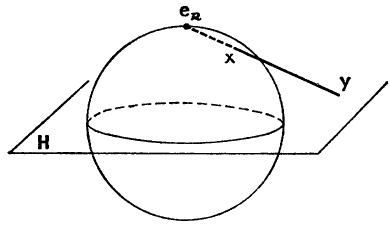
\includegraphics[keepaspectratio]{images/part001_990d2877.jpg}}\\
图 3.

若用 A 表示 \(\{e_{n}\}\) 在 \(S_{n-1}\) 中的补集，这些公式表明我们就这样定义了 A 到超平面 H 上的一个同胚。这个同胚称为 A 到 H 上的球极投影，或（滥用地说）\(S_{n-1}\) 到 H 上的球极投影；\(e_{n}\) 是投影的顶点，H 是投影超平面。更一般地，若 \(H'\) 是过 o 的任一超平面（\(B_{n}\) 的一个直径超平面），且 a 是 \(S_{n-1}\) 与过 o 而垂直于 \(H'\) 的直线的交点之一，我们就可以同样地定义以 a 为顶点、以 \(H'\) 为投影超平面的球极投影；在任何情形下，这个投影都可以通过一个把 \(H'\) 变成 H、把 a 变成 \(e_{n}\) 的正交变换化归为前一个投影。

命题 4. 若 \(n > 1\) ，欧氏球面 \(S_{n-1}\) 同胚于添加一个“无穷远点”而紧化的空间 \(\mathbf{R}^{n-1}\)（第 I 章，§ 9，第 8 小节，定理 4）。

因为球极投影定义了 \(S_{n-1}\) 中一点的补集到 \(R^{n}\) 的一个超平面上的同胚，而这个超平面同胚于 \(R^{n-1}\)。

推论 1. 球面 \(S_{n}\) 同胚于把球 \(B_{n}\) 中球面 \(S_{n-1}\) 的所有点等同起来所得到的商空间。

球 \(B_{n}\) 是正则空间（第 I 章，§ 8，第 4 小节）；因此 \(B_{n}\) 的商空间 F——把 \(S_{n-1}\) 的所有点等同起来而得到的——是豪斯多夫的（第 I 章，§ 8，第 6 小节，命题 15）。由于 \(B_{n}\) 是紧的，F 也是紧的，从而由亚历山德罗夫定理（第 I 章，§ 9，第 8 小节，定理 4），F 同胚于添加一个无穷远点而紧化的 n 维开球。因此结论由命题 2 与命题 4 得出。

推论 2. 圆周 \(\mathbf{S}_1\) 同胚于环面 \(\mathbf{T}\)。

在第 VIII 章，§ 2，第 1 小节中，我们将作为一个更精确的定理的推论重新得到这个结果。

命题 5. 若 \(n > 1\) ，欧氏球面 \(\mathbf{S}_{n-1}\) 是连通的且局部连通的，并且它的每个点都有一个同胚于 \(\mathbf{R}^{n-1}\) 的开邻域。

\(S_{n-1}\) 中一点的补集是连通的稠密集，因此（第 I 章，§ 11，第 1 小节，命题 1）\(S_{n-1}\) 是连通的。要看出每个点都有一个同胚于 \(R^{n-1}\) 的邻域，只需从一个异于该给定点的顶点作球极投影即可。

由这个命题以及第 3 小节的命题 3 推出，\(\mathbf{R}_n^*\) 作为两个连通空间的乘积是连通的（第 I 章，§ 11，第 4 小节，命题 8；参见 § 1，习题 10）。

\(S_{n-1}\) 与 \(B_{n}\) 的一个直径超平面所决定的闭（相应地，开）半空间的交，称为 \(S_{n-1}\) 的闭（相应地，开）半球面。通过到该直径超平面上的球极投影，不含投影顶点的闭（相应地，开）半球面被映成一个 n - 1 维的闭（相应地，开）球，从而同胚于它。

当 n = 2 时，我们说“半圆周”而不说“半球面”。

\section{实射影空间}

在本节中我们需要不断地引用有关商空间的概念和结果（第 I 章，§ 3），特别是下面两条性质，为方便起见我们把它们陈述为引理：

设 E 是拓扑空间，R 是 E 上的一个等价关系，A 是 E 的一个子集，\(R_{A}\) 是 R 在 A 上诱导的等价关系，f 是 E 到 E/R 上的典范映射。那么：

引理 1. 若 A 中每个关于 \(R_{A}\) 饱和的开（相应地，闭）集，都是 E 中关于 R 饱和的开（相应地，闭）集在 A 上的迹，则商空间 \(A/R_{A}\) 同胚于 E/R 的子空间 \(f(A)\)。特别地，当 A 在 E 中是开的或闭的且关于 R 饱和时，情形就是如此。

这由第 I 章，§ 3，第 6 小节，命题 10 得出。

引理 2. 若存在连续映射 \(g\) ——\(\mathbf{E}\) 到 \(\mathbf{A}\) 上的——，使得对一切 \(x \in \mathbf{E}\) ，\(g(x)\) 属于 \(x\) 的等价类，则商空间 \(\mathrm{A} / \mathrm{R}_{\mathbf{A}}\) 同胚于 \(\mathbf{E} / \mathbf{R}\)。

这就是第 I 章，§ 3，第 6 小节，命题 10 的推论 2。

\subsection{实射影空间的拓扑}

我们回忆代数中的下述定义：给定一个除环或域 \(\mathbf{K}\) ，把过 \(o\) 的直线（即一维向量子空间）——左向量空间 \(\mathbf{K}_s^{n+1}\) （\(\mathbf{K}\) 上的）中的——所成的集，称为 \(n\) 维左射影空间（\(\mathbf{K}\) 上的），记作 \(\mathbf{P}_n(\mathbf{K})\)。

若把 \(K_{s}^{n+1}\) 中过 o 的每条直线对应于同一条去掉原点的直线，我们就得到 \(\mathbf{P}_{n}(\mathbf{K})\) 到 \(K_{n+1}^{*}\) （\(\{o\}\) 在 \(K_{s}^{n+1}\) 中的补集）关于下述等价关系 \(\Delta_{n}(\mathbf{K})\) 的商上的一个双射，这个等价关系定义在 \(K_{n+1}^{*}\) 的向量 x 与 y 之间：“存在 \(t \in K\) 使得 \(t \neq o\) 且 y = tx”。在下文中我们将把 \(P_{n}(\mathbf{K})\) 与这个商集等同起来。在射影空间的理论中，我们取 N 的区间 \([o, n]\) 作为 \(K_{n+1}^{*}\) 的点的坐标的指标集。坐标 \(x_{i}\) （ \(o \leqslant i \leqslant n\) ）——\(K_{n+1}^{*}\) 中典范象为 \(x \in P_{n}(\mathbf{K})\) 的任何一点的坐标——组成所谓的点 x 的齐次坐标系。

对每个整数 \(p\) （使 \(-1 \leqslant p \leqslant n\) 的），\(\mathbf{P}_n(\mathbf{K})\) 中一个 \(p + 1\) 维向量子空间（\(\mathrm{K}_s^{n+1}\) 的，去掉原点）的典范象称为 \(p\) 维射影线性簇。\(p\) 个点（\(\mathbf{P}_n(\mathbf{K})\) 中的）组成的一个系称为自由的，如果它由 \(p\) 个点——\(\mathrm{K}_{n+1}^*\) 的、在向量空间 \(\mathrm{K}_s^{n+1}\) 中构成自由系的——的典范象组成。\(\mathbf{P}_n(\mathbf{K})\) 中由 \(p + 1\) 个点的自由系生成的射影线性簇（即包含这 \(p + 1\) 个点的最小射影线性簇）是 \(p\) 维的。

当 K 是域 R 时，相应的射影空间可以赋以拓扑，我们将研究的就是这些空间。

定义 1. 射影空间 \(\mathbf{P}_n(\mathbf{R})\) ——赋以 \(\mathbf{R}_{n+1}^*\) 的拓扑关于等价关系 \(\Delta_n(\mathbf{R})\) 的商拓扑——，称为 \(n\) 维实射影空间。

射影空间 \(\mathbf{P}_{1}(\mathbf{R})\) 称为实射影直线，\(\mathbf{P}_{2}(\mathbf{R})\) 称为实射影平面。

每当没有混淆的危险时，我们将用 \(P_{n}\) 与 \(\Delta_{n}\) 代替 \(\mathbf{P}_{n}(\mathbf{R})\) 与 \(\Delta_{n}(\mathbf{R})\)。

命题 1. 射影空间 \(P_{n}\) 是豪斯多夫的。

我们首先证明关系 \(\Delta_{n}\) 是开的（第 I 章，§ 5，第 2 小节）。设 A 是 \(\mathbf{R}_{n+1}^{*}\) 中的开集；要使 A 关于 \(\Delta_{n}\) 饱和，须取与 A 位似的诸集 \(t\mathbf{A}\) 的并，这里 \(t\) 取遍 \(\neq 0\) 的实数的集；由于这些集中每一个都是开的，它们的并也是开的。

由第 I 章，§ 8，第 3 小节的命题 8，只要证明 \(\mathbf{R}_{n+1}^{*}\times\mathbf{R}_{n+1}^{*}\) 的由关系 \(\Delta_{n}\) 定义的子集 M 是闭的，命题即得证明。设 \((x,y)\) 是 \(\mathbf{R}_{n+1}^{*}\times\mathbf{R}_{n+1}^{*}\) 中属于 M 的闭包的一点。若 \(x=(x_{i})\) ，则有指标 \(i\) 使 \(x_{i}\neq0\) ；因此存在 \((x,y)\) 的邻域 V，使得对每一点 \((x^{\prime},y^{\prime})\in\mathbf{M}\cap\mathbf{V}\) ，第 \(i\) 个坐标 \(x_{i}^{\prime}\) （\(x^{\prime}\) 的）不是 o。当 \((x^{\prime},y^{\prime})\) 保持属于 M 而趋于 \((x,y)\) 时，\(y_{i}^{\prime}x_{i}^{\prime-1}\) 趋于 \(t=y_{i}x_{i}^{-1}\) ；由于 \(y^{\prime}=(y_{i}^{\prime}x_{i}^{\prime-1})x^{\prime}\) ，取极限便见 \(y=tx\) ，这表明 \((x,y)\in\mathbf{M}\) 。

命题 2. 射影空间 \(\mathbf{P}_{n}\) 是紧的且连通的，并且同胚于球面 \(\mathbf{S}_{n}\) 关于 \(\Delta_{n}\) 在该球面上诱导的等价关系的商。

令 \(\Delta_n'\) 是 \(\mathbf{S}_n\) 上由 \(\Delta_n\) 诱导的等价关系（\(\Delta_n'\) 的等价类是 \(\mathbf{S}_n\) 的对径点对）。映射 \(x \to x/||x||\) （\(\mathbf{R}_{n+1}^*\) 到 \(\mathbf{S}_n\) 上的）是连续的，因此（引理 2）\(\mathbf{P}_n\) 同胚于 \(\mathbf{S}_n/\Delta_n'\)。由于 \(\mathbf{S}_n\) 是紧的且连通的，\(\mathbf{S}_n\) 的每个豪斯多夫商空间也是紧的且连通的（第 I 章，§ 9，第 4 小节，定理 2 的推论 1；§ 11，第 3 小节，命题 7）。

命题 3. 若 \(n \geqslant 0\) ，射影空间 \(\mathbf{P}_n\) 同胚于把球 \(\mathbf{B}_n\) 中 \(\mathbf{S}_{n-1}\) 的每个点与其对径点等同起来所得到的商空间。

设 H 是 \(S_{n}\) 的由 \(x_{0} \leqslant 0\) 定义的闭半球面。\(P_{n}\) ——它同胚于 \(S_{n}\) 关于关系 \(\Delta_{n}^{\prime}\) 的商空间——也同胚于 \(S_{n}\) 的子集 H 关于关系 \(\Delta_{n}^{\prime\prime}\) （由 \(\Delta_{n}^{\prime}\) 在 H 上诱导的）的商。由于 \(\Delta_{n}^{\prime}\) 的每个等价类都至少与 H 交于一点，因此（引理 1）只需验证：关于 \(\Delta_{n}^{\prime}\) 把 U （H 的开子集，关于 \(\Delta_{n}^{\prime\prime}\) 饱和）加以饱和化，就得到 V ——\(S_{n}\) 的一个开子集。现在，若 \(a = (a_{i}) \in U\) 且 \(a_{0} < 0\) ，则存在邻域 W （a 的，在 \(S_{n}\) 中的）含于 U，而 W 与 \(-W\) 的并是 a 的一个关于 \(\Delta_{n}^{\prime}\) 饱和且含于 V 的邻域。反之若 \(a_{0} = 0\) ，我们有 \(- a \in U\) ，且存在 r \textgreater{} o，使得点 \(x \in H\) ——满足关系 \(||x-a||<r, ||x+a||<r\) 之一的——所成的集合含于 U；点 \(x\in S_{n}\) ——满足这两个关系之一的——所成的集合就是 a 的那个关于 \(\Delta_{n}^{\prime}\) 饱和且含于 V 的邻域。

注意，商空间 \(H/\Delta_{n}^{\prime\prime}\) 是在 H 中把 \(S_{n-1}\) （即 H 与超平面 \(x_{0}=0\) 的交）的每个点与其相反点等同起来而得到的。要完成证明，只需注意以 \(e_{0}\) 为顶点的球极投影（§ 2，第 4 小节）是 H 到 \(B_{n}\) 上的同胚，且保持 \(S_{n-1}\) 的点不变。

\subsection{射影线性簇}

每个单射线性映射 \(f\) ——\(\mathbf{R}^{n+1}\) 到 \(\mathbf{R}^{m+1}\) 中的（ \(m \geqslant n\) ）——通过限制到 \(\mathbf{R}_{n+1}^*\) 再关于关系 \(\Delta_n\) 与 \(\Delta_m\) 取商（《集合论》，R，§ 5，第 8 小节），定义了一个单射映射 \(g\) ——\(\mathbf{P}_n\) 到 \(\mathbf{P}_m\) 中的——，称为射影线性映射。若 \(\varphi\) （相应地，\(\psi\)）是 \(\mathbf{R}_{n+1}^*\) 到 \(\mathbf{P}_n\) 上（相应地，\(\mathbf{R}_{m+1}^*\) 到 \(\mathbf{P}_m\) 上）的典范映射，则我们有 \(g \circ \varphi = \psi \circ f\) ，这表明 \(g\) 在 \(\mathbf{P}_n\) 上连续（第 I 章，§ 3，第 4 小节，命题 6 的推论）。特别地，\(\mathbf{P}_n\) 的每个射影线性变换（即 \(\mathbf{P}_n\) 到其自身的射影线性映射）是 \(\mathbf{P}_n\) 到其自身的一个同胚。

我们还回忆，若 V 与 \(V'\) 是两个 p 维射影线性簇（\(P_{n}\) 中的），则存在 \(P_{n}\) 的一个射影线性变换把 V 变换为 \(V'\)。特别地，若 \(p \geqslant 0\) ，则存在把 V 变换成坐标射影线性簇的射影线性变换，也就是说，变换成坐标簇 \(W'\) （\(p + 1\) 维的，\(R^{n+1}\) 的，去掉点 o 的）的典范象。若把 \(W'\) 与 \(R_{p+1}^{*}\) 等同，\(\Delta_{n}\) 在 \(W'\) 上诱导的关系正是 \(\Delta_{p}\) ；由于 \(W'\) 是闭的且关于 \(\Delta_{n}\) 饱和，引理 1 表明 \(V'\) 同胚于 \(P_{p}\) 且在 \(P_{n}\) 中是闭的；此外，若 p \textless{} n，它的补集在 \(P_{n}\) 中稠密（§ 1，第 4 小节，命题 3 的推论）。因此：

命题 4. 射影空间 \(P_{n}\) 中每个 p 维射影线性簇在 \(P_{n}\) 中是闭的，且同胚于 \(P_{p}\)；若 p \textless{} n，其补集在 \(P_{n}\) 中稠密。

这个结果是在任意除环上的射影空间中把一维与二维射影线性簇称为射影直线与射影平面这些名称的由来。我们还回忆，\(P_{n}\) 中 n - 1 维的射影线性簇称为射影超平面；每个射影超平面等同于齐次坐标满足形如 \(\sum_{i=0}^{n}a_{i}x_{i}=0\) 的关系（其中诸 \(a_{i}\) 不全为零）的点所成的集（超平面的“方程”）。

\pandocbounded{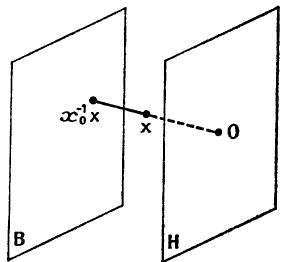
\includegraphics[keepaspectratio]{images/part001_d597a17f.jpg}}\\
图 4.

命题 5. 在射影空间 \(\mathbf{P}_n\) （ \(n \geqslant 0\)）中，射影超平面 H 的补集同胚于 \(\mathbf{R}^n\)。

作一个射影线性变换，我们可以假设 H 是方程为 \(x_{0}=0\) 的超平面。集 A ——由点 \(\boldsymbol{x}=(x_{i})\) （\(R_{n+1}^{*}\) 的，满足 \(x_{0}\neq0\) 的）组成——是开的且关于 \(\Delta_{n}\) 饱和；它的典范象 C （在 \(P_{n}\) 中的）——即 H 在 \(P_{n}\) 中的补集——因此同胚于 A 关于等价关系 \(\Theta\) （由 \(\Delta_{n}\) 在 A 上诱导的）的商（引理 1）。令 B 是方程为 \(x_{0}=1\) 的超平面（\(R^{n+1}\) 中的）。对每一点 \(x\in A\) ，使它对应于点 \(x_{0}^{-1}x\) ，即过 o 与 x 的直线和 B 的交点（图 4）；这样我们定义了 A 到 B 上的连续映射 g，使 \(g(x)\) 是 B 中与 x 模 \(\Theta\) 同余的唯一的点。由此推出 B 同胚于 A/ \(\Theta\) （引理 2），从而同胚于 C；由于 B 同胚于 \(R^{n}\) ，证明完成。

推论. \(P_{n}\) 的每个点都有一个同胚于 \(R^{n}\) 的开邻域。特别地由此推出实射影空间是局部连通的（这也可由第 I 章，§ 11，第 6 小节，命题 12 得出）。

\subsection{实数空间到射影空间中的嵌入}

第 2 小节的命题 5 表明，若在 \(P_{n}\) （ \(n \geqslant 0\)）中给定一个射影超平面 H ，就存在 \(R^{n}\) 到该超平面的补集 \(\complement H\) 上的一个同胚。一旦选定了 H ，用命题 5 中定义的同胚把 \(R^{n}\) 与 \(\complement H\) 等同起来常常是方便的；这时称射影超平面 H 位于“无穷远”，它的点和子集也是如此。通常取 H 为方程为 \(x_{0}=0\) 的“坐标”超平面，于是点 \(z=(z_{i})\) （\(R^{n}\) 的）就与 \(P_{n}\) 中齐次坐标为 \(1, z_{1}, z_{2}, \ldots, z_{n}\) 的点等同。

一旦作了这个等同，在 \(P_{n}\) 中，任何仿射线性簇 V （p 维的，\(R^{n}\) 中的）的闭包是一个 p 维射影线性簇，不含于无穷远超平面中，且等同于由 V 生成的射影线性簇。反之，每个射影线性簇 P （p 维的，不含于无穷远超平面的）在 \(R^{n}\) 上的迹是一个 p 维仿射线性簇，它在 \(P_{n}\) 中的闭包就是 P。

在特例 \(n = 1\) ，无穷远超平面是一个点；由于 \(\mathbf{P}_1\) 是紧的，由亚历山德罗夫定理（第 I 章，§ 9，第 8 小节，定理 4），\(\mathbf{P}_1\) 同胚于空间 \(\tilde{\mathbf{R}}\) ——由局部紧空间 \(\mathbf{R}\) 添加一个点（“无穷远点”）而紧化所得到的——。由 § 2 第 4 小节的命题 4，我们还看出实射影直线 \(\mathbf{P}_1(\mathbf{R})\) 同胚于圆周 \(\mathbf{S}_1\) 以及环面 \(\mathbf{T}\)。

另一方面，若 \(n > 1\) ，\(\mathbf{P}_n(\mathbf{R})\) 不同胚于 \(\mathbf{S}_n\) ，这一点我们以后将会看到（参见习题 4）。

空间 \(\tilde{R}\) 的“无穷远点”记作 \(\infty\) ，不带正负号。重要的是不要把 \(\tilde{R}\) 与第 IV 章，§ 4 中定义的扩充实直线 \(\overline{R}\) 相混淆，后者有两个“无穷远点”；事实上，\(\tilde{R}\) 同胚于 \(\overline{R}\) 的商空间——把两点 \(+\infty\) 与 \(-\infty\) 等同起来所得到的。

\subsection{在实值函数的延拓中的应用}

由于 \(\mathbf{R}\) 可以看作 \(\tilde{\mathbf{R}}\) 的一个子集，每个集 \(\mathbf{E}\) 到 \(\mathbf{R}\) 中的映射（即 \(\mathbf{E}\) 上的每个实值函数）都可以看作 \(\mathbf{E}\) 到 \(\tilde{\mathbf{R}}\) 中的映射；特别地，若 \(\mathbf{E}\) 是拓扑空间 \(\mathbf{F}\) 的子集，且 \(f\) 是 \(\mathbf{E}\) 到 \(\mathbf{R}\) 中的映射，则可能发生这样的情形：在闭包 \(\overline{\mathbf{E}}\) ——\(\mathbf{E}\) 的闭包——的某些点处，\(f(x)\) 趋于极限 \(\infty\) （当 \(x\) 保持属于 \(\mathbf{E}\) 而趋于这些点之一时）；这时我们就可以把函数 \(f\) 连续延拓，在这些点处给它值 \(\infty\)（第 I 章，§ 8，第 5 小节，定理 1）。

特别地考察 E 是 \(R^{n}\) 的子集的情形，这时空间 \(R^{n}\) 本身看作嵌入在射影空间 \(P_{n}\) 中；若假设无穷远超平面是 \(x_{0}=0\) ，定义在 E 上的实值函数 f 就可以等同于映射

\[
(x _ {0}, x _ {1}, x _ {2}, \ldots , x _ {n}) \rightarrow f \left(\frac {x _ {1}}{x _ {0}}, \frac {x _ {2}}{x _ {0}}, \ldots , \frac {x _ {n}}{x _ {0}}\right)
\]

（E 到 \(\tilde{R}\) 中的映射）；由上一段所说的，这个函数可能不仅可以在 E 的闭包中的 \(R^{n}\) 的某些点处延拓，而且可以在 E 的闭包中 \(P_{n}\) 的某些“无穷远点”处延拓。

让我们证明，用这个方法可以得到例如代数中已经定义的一个实变量的有理函数到整个 \(\tilde{\mathbf{R}}\) 上的连续延拓。让我们把 \(\tilde{\mathbf{R}}\) 与 \(\mathbf{P}_1\) 等同起来，每个实数 \(x \in \mathbb{R}\) 等同于齐次坐标为 (1, x) 的点，而点 \(\infty\) 等同于齐次坐标为 (0,1) 的点。设 \(u(x)/v(x)\) 是一个有理函数，\(u\) 与 \(v\) 是次数分别为 \(m\) 与 \(n\) 的两个互素多项式；若例如假设 \(m \leqslant n\) ，并令 \(u_1(x,y) = x^n u(y/x)\) ，\(v_1(x,y) = x^n v(y/x)\) ，则有理函数 \(u/v\) ——在由实数 \(x\) （满足 \(v(x) \neq 0\) 的）组成的集上——可以看作映射 \((x,y) \to (v_1(x,y), u_1(x,y))\) 的限制。换句话说，我们把 \(u/v\) 连续延拓，给它值 \(\infty\) 于那些点 \(x \in \mathbb{R}\) ——使 \(v(x) = 0\) 的——处，并在点 \(\infty\) 处给它值 \(0\) （若 \(m < n\)）、值 \(\infty\) （若 \(m > n\)）、或首项系数之比（若 \(m = n\)）。

特别地，函数 \(1 / x\) 可以延拓到点 \(o\) ，在那里取值 \(\infty\) ，也可延拓到 \(\infty\) ，在那里取值 \(o\) ；这个延拓了的函数显然是 \(\tilde{\mathbf{R}}\) 到其自身的一个同胚。分式线性函数 \((ax + b) / (cx + d)\) （当 \(ad - bc \neq o\) 时）亦然。

同样，若 \(n\) 是 \(> 0\) 的整数，函数 \(x^n\) 可延拓到点 \(\infty\) ，在那里取值 \(\infty\)。

另一方面，两个实变量的有理函数一般不可能连续延拓到空间 \(\mathbf{P}_1 \times \mathbf{P}_1\) 或空间 \(\mathbf{P}_2\)（参见习题 5）。

\subsection{射影线性簇的空间}

给定一个除环 K，集 \(\mathbf{P}_{n,p}(\mathbf{K})\) ——\(p \geqslant 0\) 维射影线性簇（左射影空间 \(\mathbf{P}_{n}(\mathbf{K})\) 的）组成的集——显然与 \(p + 1\) 维向量子空间（左向量空间 \(K_{s}^{n+1}\) 的）组成的集一一对应。令 \(L_{n+1, p+1}(\mathbf{K})\) 表示自由系 \((x_{k})_{1 \leqslant k \leqslant p+1}\) ——\(p + 1\) 个向量（\(K_{s}^{n+1}\) 中的）组成的自由系——所成的集；那么集 \(\mathbf{P}_{n,p}(\mathbf{K})\)

仍然与 \(\mathbf{L}_{n+1,p+1}(\mathbf{K})\) 关于下述等价关系 \(\Delta_{n,p}(\mathbf{K})\) 的商一一对应：“\((\mathbf{x}^{k})\) 与 \((\mathbf{y}^{k})\) 生成同一个 \(p+1\) 维向量子空间（\(K_{s}^{n+1}\) 的）”。在下文中我们将把 \(\mathbf{P}_{n,p}(\mathbf{K})\) 与这个商集等同。另一方面，若把每个自由系 \((\mathbf{x}_{k})\) ——\(p+1\) 个向量（\(K_{s}^{n+1}\) 中的）组成的——对应于矩阵 X ——\(p+1\) 行 \(n+1\) 列的，以 \(x_{k}\) 为第 k 行（ \(1\leqslant k\leqslant p+1\) ）——，我们就得到 \(L_{n+1,p+1}(\mathbf{K})\) 与所有 \(p+1\) 行 \(n+1\) 列、秩为 \(p+1\) 的矩阵组成的集之间的一一对应；我们将把 \(L_{n+1,p+1}(\mathbf{K})\) 与这个矩阵集等同，而两个矩阵 X, Y 之间的关系 \(\Delta_{n,p}(\mathbf{K})\) 就是：“存在 \(p+1\) 阶非奇异方矩阵 T 使得 Y = T.X”。

在下文中我们取 K 为域 R，并在上述记号中省略字母 K。我们可以用一种推广实射影空间拓扑定义的办法来定义 \(P_{n,p}\) 上的拓扑。即，\(L_{n+1, p+1}\) 含于空间 \(M_{p+1, n+1}\) ——以实数为元素的 \(p + 1\) 行 \(n + 1\) 列的一切矩阵组成的空间——；我们给 \(L_{n+1, p+1}\) 赋以这个矩阵空间的拓扑所诱导的拓扑（§ 1，第 6 小节）。

定义 2. 空间 \(\mathbf{P}_{n,p}\) ——拓扑空间 \(\mathbf{L}_{n+1,p+1}\) 关于等价关系 \(\Delta_{n,p}\) 的商——称为 \(p\geqslant0\) 维射影线性簇（在实射影空间 \(\mathbf{P}_{n}\) 中的）的空间。

我们将使用下述记号：给定一个 \(p + 1\) 行 \(n + 1\) 列的矩阵 X，以及任一严格递增序列

\[
\sigma = (i _ {1}, \dots , i _ {p + 1})
\]

的 \(p + 1\) 个指标（区间 \([0, n]\) ，属于 \(\mathbf{N}\) ），我们用 \(X_{\sigma}\) 表示 \(X\) 的由指标为 \(i_1, i_2, \ldots, i_{p+1}\) 的列组成的方子矩阵。我们用 \(\mathbf{A}_{\sigma}\) 表示 \(\mathbf{L}_{n+1, p+1}\) 中由这些矩阵 \(X\) ——使 \(X_{\sigma}\) 非奇异的——组成的子集。由 § 1 第 6 小节的命题 6，\(\mathbf{A}_{\sigma}\) 是 \(\mathbf{M}_{p+1, n+1}\) 中的稠密开集，而且函数 \(X \to X_{\sigma}^{-1}\) 在 \(\mathbf{A}_{\sigma}\) 上连续。

集 \(A_{\sigma}\) 的一个几何解释如下：设 \(E_{\sigma}\) 是 \(R^{n+1}\) 中由典范基的向量 \(e_{i}\) （使 \(i \in \sigma\) 的）生成的向量子空间，设 \(E_{\sigma}'\) 是由 \(e_{i}\) （使 \(i \notin \sigma\) 的）生成的余子空间；那么说矩阵 x 属于 \(A_{\sigma}\) ，意思是其在 \(E_{\sigma}\) 上的投影——它的 \(p + 1\) 行（即 \(x_{k}\)）的投影——构成自由系，或者说，由诸 \(x_{k}\) 生成的向量子空间是 \(E_{\sigma}'\) 的余子空间（或者说它与 \(E_{\sigma}'\) 的交只由 o 组成）。

命题 6. 空间 \(\mathbf{P}_{n,p}\) 是豪斯多夫的。

我们首先证明关系 \(\Delta_{n,p}\) 是开的。若 U 是 \(L_{n+1,p+1}\) 中的开集，要使 U 关于 \(\Delta_{n,p}\) 饱和，须取 U 在映射 \(X \to T \cdot X\) 下的象的并，这里 T 取遍 \(p + 1\) 阶非奇异方矩阵的集；由于这些映射中每一个都是双连续的，所有这些象都是开集，因此它们的并也是开集。

由第 I 章，§ 8，第 3 小节的命题 8，只要证明 \(L_{n+1,p+1} \times L_{n+1,p+1}\) 的由 \(\Delta_{n,p}\) 定义的子集 N 是闭的，证明即告完成。设 \((X,\mathcal{Y})\) 是乘积空间中属于 N 的闭包的一点，设 \(\sigma\) 是使 \(X_{\sigma}\) 非奇异的指标序列：由于 \(A_{\sigma}\) 是开的，存在 \((X,\mathcal{Y})\) 的邻域 V，使得对每对 \((X',\mathcal{Y}') \in \mathrm{N} \cap \mathrm{V}\) ，矩阵 \(X'_{\sigma}\) 都是非奇异的；当 \((X',\mathcal{Y}')\) 保持属于 N 而趋于 \((X,\mathcal{Y})\) 时，矩阵 \(Y'_{\sigma}X_{\sigma}^{\prime -1}\) 就趋于 \(T = Y_{\sigma}X_{\sigma}^{-1}\) ；由于我们有 \(Y' = (Y'_{\sigma}X_{\sigma}^{\prime -1})X'\) ，取极限便见 Y = T.X，证明完成。

命题 7. 空间 \(\mathbf{P}_{n,p}\) 是紧的。

只需证明存在 \(L_{n+1, p+1}\) 的一个紧子空间，它与模 \(\Delta_{n,p}\) 的每个等价类至少交于一点；因为这时 \(P_{n,p}\) 是这个子空间在 \(L_{n+1, p+1}\) 到 \(P_{n,p}\) 上的典范映射下的象，因此是紧的（第 I 章，§ 9，第 4 小节，定理 2）。

令 \(\mathbf{V}_{n+1, p+1}\) 是 \(\mathbf{L}_{n+1, p+1}\) 的这样的子空间：其元素是系 \((\boldsymbol{x}_k)\) ——由 \(p + 1\) 个向量组成的——，这些向量构成它们所生成的向量子空间的欧氏标准正交基，也就是说满足 \((x_h | x_k) = 0\) （每当 \(h \neq k\) ），且 \((x_h | x_h) = 1\) （对 \(1 \leqslant h \leqslant p + 1\) ）。每个 \(p + 1\) 维向量子空间（\(\mathbf{R}^{n+1}\) 的）都有这样一个基，因此模 \(\Delta_{n,p}\) 的每个类都与 \(\mathbf{V}_{n+1, p+1}\) 相交。另一方面，矩阵 \(X = (x_{ij})\) ——\(\mathbf{V}_{n+1, p+1}\) 的——由下述关系定义

\[
\sum_ {j = 0} ^ {n} x _ {i j} ^ {2} = 1 (1 \leqslant i \leqslant p + 1),
\]

\[
\sum_ {j = 0} ^ {n} x _ {i j} x _ {k j} = 0 \quad (i \neq k);
\]

因此它们组成 \(M_{p+1, n+1}\) 中的一个闭集；又由于这些关系蕴含 \(|x_{ij}| \leqslant 1\) （对每对指标 \((i, j)\) ），这个集是有界的，从而是紧的。

命题 8. \(\mathbf{P}_{n,p}\) 是连通的且局部连通的，并且每个点都有一个同胚于 \(\mathbf{R}^{(p+1)(n-p)}\) 的开邻域。

对每个（严格递增的）指标序列 \(\sigma\) ，集 \(\mathbf{A}_{\sigma}\) 在 \(\mathbf{L}_{n+1, p+1}\) 中是开的且关于 \(\Delta_{n,p}\) 饱和；它的典范象

\(C_{\sigma}\) （\(P_{n,p}\) 中的）因此是一个开集，同胚于 \(A_{\sigma}\) 关于等价关系 \(\Theta_{\sigma}\) （在 \(A_{\sigma}\) 上由 \(\Delta_{n,p}\) 诱导的）的商（引理 1）。

令 \(\mathbf{B}_{\sigma}\) 是 \(\mathbf{A}_{\sigma}\) 中由矩阵 \(X\) ——使 \(X_{\sigma}\) 为 \(p + 1\) 阶单位矩阵的——组成的子集；\(X\) 中除 \(X_{\sigma}\) 的元素以外的元素这时是任意的，因此 \(\mathbf{B}_{\sigma}\) 同胚于空间 \(\mathbf{R}^{(p + 1)(n - p)}\) 。对每个矩阵 \(X \in \mathbf{A}_{\sigma}\) ，使它对应于矩阵 \(\Upsilon = X_{\sigma}^{-1}X\) ，它属于 \(\mathbf{B}_{\sigma}\) ；这样我们就定义了连续映射 \(g\) ——\(\mathbf{A}_{\sigma}\) 到 \(\mathbf{B}_{\sigma}\) 上的——，使 \(g(X)\) 是 \(\mathbf{B}_{\sigma}\) 中与 \(X\) 模 \(\Theta_{\sigma}\) 同余的唯一的矩阵。由此推出 \(\mathbf{B}_{\sigma}\) 同胚于 \(\mathbf{A}_{\sigma}/\Theta_{\sigma}\) （引理 2），从而同胚于 \(\mathbf{C}_{\sigma}\) 。

集 \(C_{\sigma}\) 因此是连通的。由于 \(A_{\sigma}\) 在 \(L_{n+1, p+1}\) 中稠密，\(C_{\sigma}\) 在 \(P_{n, p}\) 中稠密，因此 \(P_{n, p}\) 也是连通的（第 I 章，§ 11，第 1 小节，命题 1）。另一方面，\(P_{n, p}\) 的每个点都属于 \(C_{\sigma}\) （对至少一个指标序列 \(\sigma\) ），从而有一个同胚于 \(\mathbf{R}^{(p+1)(n-p)}\) 的开邻域。

矩阵 \(Y=g(X)\) 可以解释如下：为简单起见，设序列 \(\sigma\) 由 \(p+1\) 个指标 n-p, \(n-p+1\) , \(\ldots\) , n 组成，并用 \(a_{ij}\) ( \(1\leqslant i\leqslant p+1\) , \(o\leqslant j\leqslant n-p-1\) ) 表示 y 的前 n-p 列的元素；那么由 x 的行生成的 \(R^{n+1}\) 的向量子空间就是由方程

\[
x _ {j} = \sum_ {i = 1} ^ {p + 1} a _ {i j} x _ {n - p + i - 1} \quad (0 \leqslant j \leqslant n - p - 1).
\]

\subsection{格拉斯曼流形}

若 K 是一个域，X 是 \(\mathrm{L}_{n+1,p+1}(\mathrm{K})\) 的任一矩阵，令 \(c_{\sigma}(X)\) 表示 \(X_{\sigma}\) 的行列式；这样，对 \(\mathrm{L}_{n+1,p+1}(\mathrm{K})\) 的每个矩阵 X 就对应

\[
h = \binom {n + 1} {p + 1}
\]

个行列式，它们不全为零（\(p + 1\) 行——\(X\) 的——的外积的分量）。若把 \(X\) 对应到射影空间 \(\mathbf{P}_{h-1}(\mathbf{K})\) 中齐次坐标为诸 \(c_{\sigma}(X)\) 的点，我们就定义了 \(\mathbf{L}_{n+1,p+1}(\mathbf{K})\) 到 \(\mathbf{P}_{h-1}(\mathbf{K})\) 中的一个映射，它与关系 \(\Delta_{n,p}(\mathbf{K})\) 相容；取商，我们因此得到映射 \(f\) ——\(\mathbf{P}_{n,p}(\mathbf{K})\) 到 \(\mathbf{P}_{h-1}(\mathbf{K})\) 中的——。这个映射的象 \(\mathbf{G}_{n,p}(\mathbf{K})\) （\(\mathbf{P}_{n,p}(\mathbf{K})\) 在该映射下的象）称为指标 \(n\) 、\(p\) 的格拉斯曼流形。我们还回忆映射 \(f\) 是单射的，因为若 \(X\) 是使 \(X_{\sigma}\) 非奇异的矩阵，则矩阵 \(\Upsilon = X_{\sigma}^{-1}X\) ——\(\mathbf{B}_{\sigma}\) 中对应于 \(X\) 模 \(\Delta_{n,p}(\mathbf{K})\) 的类的——就是矩阵 \((d_{ij}/c_{\sigma}(X))\) ( \(1 \leqslant i \leqslant p + 1\) , \(0 \leqslant j \leqslant n\) )，其中 \(d_{ij}\) 表示从 \(X_{\sigma}\) 出发、把 \(X_{\sigma}\) 的第 i 列换成 X 的第 j 列所得矩阵的行列式{[}这蕴含 \(d_{ij}\) 与诸 \(c_{\tau}(X)\) 之一相差一个正负号{]}。

当 \(\mathbf{K}\) 是域 \(\mathbf{R}\) 时，这个映射 \(f\) 显然是连续的。逆映射 \(g\) 也是连续的；因为 \(\mathbf{B}_{\sigma}\) 中的矩阵的元素是它所对应的格拉斯曼流形的点的齐次坐标的有理函数；由于 \(f(\mathbf{B}_{\sigma}) = \mathbf{B}_{\sigma}'\) 是 \(\mathbf{G}_{n,p}\) 中指标为 \(\sigma\) 的齐次坐标不为 \(0\) 的点的集，它是 \(\mathbf{G}_{n,p}\) 中的开集；因此 \(g\) 在 \(\mathbf{B}_{\sigma}'\) 的每一点连续，又由于 \(\mathbf{G}_{n,p}\) 的每一点都属于至少一个集 \(\mathbf{B}_{\sigma}'\) ，\(g\) 在每一点都连续。于是：

命题 9. 格拉斯曼流形 \(\mathbf{G}_{n,p}\) 同胚于空间 \(\mathbf{P}_{n,p}\)。

最后我们回忆，格拉斯曼流形 \(\mathbf{G}_{n,p}(\mathbf{K})\) 与 \(\mathbf{G}_{n,n-p-1}(\mathbf{K})\) 是同一射影空间 \(\mathbf{P}_{h-1}(\mathbf{K})\) 的子集，并且可以通过一个射影线性变换互相变换；由此推出 \(G_{n,p}\) 与 \(G_{n,n-p-1}\) 是同胚的。

\ExerciseGroupsStart
\ExerciseSection

\begin{enumerate}
\def\labelenumi{\arabic{enumi})}
\item
  试证明 \(\mathbf{R}^n\) 与 \(\mathbf{R}\) 等势，利用康托尔定理（第 IV 章，§ 8，第 6 小节，定理 1）以及关系式 \(2^{\mathfrak{a}} \cdot 2^{\mathfrak{a}} = 2^{\mathfrak{a}}\) （它对一切无限基数 \(\mathfrak{a}\) 成立）。
\item
  存在区间 \(\mathbf{I} = [\mathrm{o},\mathrm{i}]\) （ \(\mathbf{R}\) 的）到正方形 \(\mathbf{I}\times \mathbf{I}\) （ \(\mathbf{R}^2\) 的）上的连续映射（“佩亚诺曲线”，参见习题 8）。（首先借助第 IV 章，§ 8 的习题 11 证明存在连续映射 \(f\) ，它把康托尔三分集 \(\mathbf{K}\) 映到 \(\mathbf{I}\times \mathbf{I}\) 上，然后把 \(f\) 延拓到 \(\mathbf{I}\) 上。）
\item
  设 A 与 B 是 \(R^{2}\) 的两个可数稠密子集。证明：存在 \(R^{2}\) 到其自身的同胚，它把 A 变换成 B。（首先证明：借助一个旋转，可以化归为投影 \(pr_{1}\) 与 \(pr_{2}\) 都是 A 与 B 到 R 中的单射映射的情形。然后，用一个适当的归纳程序，定义 A 到 B 上的一个双射，它决定 \(pr_{1}A\) 到 \(pr_{1}B\) 上的一个单调映射以及 \(pr_{2}A\) 到 \(pr_{2}B\) 上的一个单调映射。最后，利用第 IV 章，§ 2 的习题 11，证明这个映射是一个同胚，并且可以延拓为 \(R^{2}\) 到其自身的同胚。）由此推出：若 C 是 \(R^{2}\) 的一个子集，它的补集稠密，则 C 同胚于 \(Q^{2}\) 在 \(R^{2}\) 中的补集的一个子集。把这些结果推广到 \(R^{n}\) ，n \textgreater{} 2。
\item
  \(\mathbf{R}^n\) 的每个没有孤立点的可数子空间都同胚于有理直线 \(\mathbf{Q}\) （应用第 IV 章，§ 8 的习题 13）。
\item
  \(\mathbf{R}^n\) 的每个没有孤立点的全不连通紧子空间都同胚于康托尔三分集（利用第 IV 章，§ 8 的习题 11 与习题 12，以及第 II 章，§ 4，第 4 小节的命题 6）。
\item
  \(R^{n}\) 的子集 L 称为折线，如果存在点的有限序列 \((x_{i})_{0\leqslant i\leqslant p}\) （由 \(R^{n}\) 中的点组成），使得：若用 \(S_{i}\) 表示以 \(x_{i-1}\) 与 \(x_{i}\) 为端点的线段（ \(i\leqslant i\leqslant p\) ），则 L 是诸 \(S_{i}\) 的并，这些线段称为 L 的边。（一般地，定义同一条折线的 \(R^{n}\) 中点的有限序列有无穷多个。）折线也是 {[}o, i{]} 到 \(R^{n}\) 中的映射 u 的象：存在一个严格递增序列 \((t_{j})_{0\leqslant j\leqslant q}\) （在 {[}o, i{]} 中取值），\(t_{0}=0\) 且 \(t_{q}=1\) ，使得 u 是仿射线性映射
\end{enumerate}

\[
t \rightarrow \boldsymbol {a} _ {j} + t \boldsymbol {b} _ {j} \quad \text { for } \quad t _ {j - 1} \leqslant t \leqslant t _ {j} \quad \text { and } \quad i \leqslant j \leqslant q
\]

（这样的映射 \(u\) 称为“分段线性的”。）给定 \(\mathbf{R}^n\) 的一个非空子集 A，我们说 A 的两点 \(a, b\) 在 A 中可用折线连结，如果存在折线 \(L \subset A\) ，它由一个序列 \((x_i)_{0 \leqslant i \leqslant p}\) 定义，使得 \(x_0 = a\) 且 \(x_p = b\) 。若 A 的任意两点都能在 A 中用折线连结，则 A 是连通的。反之，若 A 是 \(\mathbf{R}^n\) 的连通开子集，证明 A 的任意两点都能在 A 中用折线连结（考察关系“ \(x\) 与 \(y\) 在 A 中可用折线连结”（它是 A 的点 \(x, y\) 之间的关系）；证明这是一个等价关系，而且它的类都是开集）；甚至可以始终假设这条折线是一些线段的并，其中每条线段都平行于某条坐标轴（同样的方法）。由此推出：若 A 是 \(\mathbf{R}^n\) 中的非空开集，则点 \(a \in A\) 的分支是 A 中能与 \(a\) 用 A 中折线连结的一切点组成的集。

\begin{enumerate}
\def\labelenumi{\arabic{enumi})}
\setcounter{enumi}{6}
\item
  设 A 是 \(R^{n}\) 中的非空连通开集（n \textgreater{} 1），并设 \((\mathrm{V}_{p})_{p \in \mathbb{N}}\) 是 \(R^{n}\) 中线性簇的一个可数族，其中每个线性簇的维数都 \(\leqslant n - 2\) 。证明：若 B 是诸 \(V_{p}\) 的并，则 \(A \cap \mathfrak{C}B\) 在 A 中稠密且连通。（为证明 \(A \cap \mathfrak{C}B\) 在 A 中稠密，对 n 用归纳法。然后证明：若 x, y 是 A 的两个不同的点，则对每个 \(\varepsilon > 0\) 存在点 \(y' \in A\) 满足 \(||y' - y|| \leqslant \varepsilon\) ，并且以 x 与 \(y'\) 为端点的闭线段与 B 只交于点 x。最后利用习题 6 证明 \(A \cap \mathfrak{C}B\) 连通。）
\item
  由习题 7 推出：若 \(n > \mathbf{I}\) ，则 \(\mathbf{R}^n\) 的非空开子集不与 \(\mathbf{R}\) 的任何子集同胚（*）。
\item
  \(\mathbf{R}^{n}\ (n > \mathrm{i})\) 中的折线 L（习题 6）称为简单折线，如果它同胚于 R 的区间 \(I = [0, i]\)。这等价于说存在 I 到 L 上的一个分段线性同胚 u（习题 6）。证明：若 A 是 \(\mathbf{R}^2\) 中的连通开集，且 \(\mathbf{L}\subset\mathbf{A}\) 是简单折线，则 \(\mathbf{A}-\mathbf{L}\) 连通（对组成 L 的线段的个数用归纳法论证，并利用第 I 章，§ 11 的习题 6）。
\end{enumerate}

* 10) a) 设 M 是有限集，R \(x, y\) 是 M 的元素 x, y 之间的一个对称关系。假设 M 中存在两个不同的元素 a, b，它们具有下列性质：存在 x ≠ a 与 y ≠ b，使得 x（相应地 y）是使 R \(a, z\) （相应地 R \(b, z\) ）为真的唯一的元素 z ∈ M；并且对 M 中每个异于 a 与 b 的 t，使 R \(t, z\) 为真的所有 z ∈ M 组成的集是一个由两个都异于 t 的元素组成的集。证明：在这些条件下，存在一个双射 i → x\_i （从 N 的区间 {[}o, n{]} 到 M 上），使得 x\_0 = a，x\_n = b，并且对 i ≤ i ≤ n，R \(x_{i-1}, x_i\) 为真（对 i 用归纳法定义 x\_i）。

\begin{enumerate}
\def\labelenumi{\alph{enumi})}
\setcounter{enumi}{1}
\tightlist
\item
  在 \(\mathbf{R}^n\) （ \(n \geqslant 2\) ）中——把它与 \(\mathbf{R}^{n-1} \times \mathbf{R}\) 等同起来——设 \(\mathbf{L}\) 与 \(\mathbf{L}'\) 是两条折线，分别由序列 \((\boldsymbol{x}_i)_{0 \leqslant i \leqslant p}\) 与 \((\boldsymbol{x}_j')_{0 \leqslant j \leqslant q}\) 定义，且具有下列性质：(i) 若记 \(\boldsymbol{x}_i = (\boldsymbol{y}_i, z_i)\) ，\(\boldsymbol{x}_j' = (\boldsymbol{y}_j', z_j')\) ，则我们有 \(z_0 = z_0' = 0\) ，\(z_p = z_q' = 1\) ，且 \(0 < z_i < 1\) 对 \(1 \leqslant i \leqslant p - 1\) 成立，\(0 < z_j' < 1\) 对 \(1 \leqslant j \leqslant q - 1\) 成立；(ii) \(p + q - 2\) 个数 \(z_i, z_j'\) （ \(1 \leqslant i \leqslant p - 1\) ，\(1 \leqslant j \leqslant q - 1\) ）两两不同；(iii) \(\mathbf{L}\) （相应地 \(\mathbf{L}'\) ）的两条不同的边至多有一个公共点{[}这个点可以是、也可以不是诸 \(\boldsymbol{x}_i\) （相应地 \(\boldsymbol{x}_j'\) ）之一{]}。证明：存在两个满射的分段线性映射（习题 6）\(\boldsymbol{u}\) ： \(\mathbf{I} \to \mathbf{L}\) ，\(\boldsymbol{u}'\colon \mathbf{I} \to \mathbf{L}'\) ，其中 \(\mathbf{I}\) 是区间 \([0, 1]\) （ \(\mathbf{R}\) 中的），使得：若记 \(\boldsymbol{u}(t) = (\boldsymbol{v}(t), \zeta(t))\) ，\(\boldsymbol{u}'(t) = (\boldsymbol{v}'(t), \zeta'(t))\) （ \(t \in \mathbf{I}\) ），则我们有 \(\zeta(t) = \zeta'(t)\) （对一切 \(t \in \mathbf{I}\) ），
\end{enumerate}

\[
\zeta (\mathrm{o}) = \zeta^ {\prime} (\mathrm{o}) = \mathrm{o} \quad \text { and } \quad \zeta (\mathrm{i}) = \zeta^ {\prime} (\mathrm{i}) = \mathrm{i}.
\]

{[}设 \((a_{k})_{1\leqslant k\leqslant p + q - 2}\) 是由异于 o 与 i 的诸 \(z_{i}\) 与诸 \(z_j^{\prime}\) 组成的严格递增序列，并令 \(a_0 = 0\) ，\(a_{p + q - 1} = \mathrm{i}\) ；设 \(\mathbf{B}_i\) 表示由满足下列条件的所有 \(\pmb {x} = (\pmb {y},z)\in \mathbb{R}^n\) 组成的集：

\[
a _ {i - 1} \leqslant z \leqslant a _ {i} \quad (\mathrm{I} \leqslant i \leqslant p + q - \mathrm{I});
\]

设 \(\mathfrak{M}\) 表示所有偶 \(\gamma = (\mathrm{C},\mathrm{C}^{\prime})\) 组成的集，其中 \(\mathrm{C}\) （相应地 \(\mathrm{C}'\) ）是同一个 \(\mathbf{B}_i\) 与 \(\mathbf{L}\) （相应地 \(\mathbf{L}'\) ）的一条边的交，且 \(\mathbf{C}\) 与 \(\mathbf{C}'\) 都不由单独一个点组成；又设 \(\mathbf{R}\wr \alpha, \beta\wr\) 表示元素 \(\alpha, \beta\) （ \(\mathfrak{M}\) 的）之间的下述关系：“ \(\alpha \neq \beta\) ；若 \(\alpha = (\mathrm{C}_1,\mathrm{C}_1')\) ，\(\beta = (\mathrm{C}_2,\mathrm{C}_2')\) ，则 \(\mathrm{C}_1 \cap \mathrm{C}_2\) 与 \(\mathrm{C}_1' \cap \mathrm{C}_2'\) 都非空，其中之一由单独一个点组成，而且若这个点不是诸 \(x_i\) （相应地 \(x_j'\) ）之一，则 \(\mathrm{C}_1\) 与 \(\mathrm{C}_2\) （相应地 \(\mathrm{C}_1'\) 与 \(\mathrm{C}_2'\) ）都含于 \(\mathbf{L}\) （相应地 \(\mathbf{L}'\) ）的同一条边中。证明 \(a\) ) 可应用于关系 \(\mathbf{R}.\) {]}

\begin{enumerate}
\def\labelenumi{\alph{enumi})}
\setcounter{enumi}{2}
\tightlist
\item
  在 \(\mathbf{R}^n\) 中（把它与 \(\mathbf{R}^{n-1} \times \mathbf{R}\) 等同起来），设 \(\mathbf{K}\) 是连通紧集，使得 \(\mathbf{K} \cap (\mathbf{R}^{n-1} \times \{\mathbf{o}\})\) 至少含两个不同的点。证明：若 \(\mathbf{K}' = \mathbf{K} - \mathbf{K}\) （即所有 \(x - y\) 组成的集，其中 \(x \in \mathbf{K}\) 且 \(y \in \mathbf{K}\) ），则 \(\mathbf{K}' \cap (\mathbf{R}^{n-1} \times \{\mathbf{o}\})\) 含有一个不由单独一个点组成的连通集。{[}利用 b)，并应用第 II 章，§ 4 的命题 6 与习题 15。{]}
\end{enumerate}

\begin{enumerate}
\def\labelenumi{\arabic{enumi})}
\setcounter{enumi}{10}
\tightlist
\item
  把第 IV 章，§ 8 的习题 14 与习题 15 推广到空间 \(\mathbf{R}^n\) （ \(n \geqslant 2\) ）。
\end{enumerate}

* 12) a) 设 \(f\) 是 \(\mathbf{R}\) 到 \(\mathbf{R}\) 中的映射，并设 \(\mathbf{G} \subset \mathbf{R}^2\) 是 \(f\) 的图象。假设 \(\mathbf{G}\) 在 \(\mathbf{R}^2\) 中稠密，并且与 \(\mathbf{R}^2\) 中每个不完全含于形如 \(\{x_n\} \times \mathbf{R}\) 的直线的可数并中的完全集相交。证明 \(\mathbf{G}\) 连通。（若不然，证明：存在两个非空的不相交开集 \(\mathbf{A}\) ，\(\mathbf{B}\) （ \(\mathbf{R}^2\) 中的），使得 \(\mathbf{G}\) 是 \(\mathbf{G} \cap \mathbf{A}\) 与 \(\mathbf{G} \cap \mathbf{B}\) 的并，\(\mathbf{A}\) 中至少有一点与 \(\mathbf{B}\) 中的一点有相同的横坐标（利用 \(\mathbf{R}\) 连通这一事实）；然后利用习题 11。）

\begin{enumerate}
\def\labelenumi{\alph{enumi})}
\setcounter{enumi}{1}
\tightlist
\item
  由 a) 推出：存在 R 到 R 中的线性映射 f，它的图象 G 在 \(R^{2}\) 中稠密且连通。{[}利用 a) 与习题 11，按照《集合论》第 III 章，§ 6 习题 24 中的同样方法，用超限归纳法定义 f 在 R 的一个哈梅尔基的各点上的值。{]}由此推出：\(R^{2}\) 的子群 G 满足第 V 章，§ 3 习题 4 中的条件 ( \(R_{I}\) ) 与 ( \(R_{II}\) ) ，但不是局部紧的，因而它的拓扑严格细于 R 的通常拓扑；并且 G 不是局部连通的。
\end{enumerate}

\begin{enumerate}
\def\labelenumi{\arabic{enumi})}
\setcounter{enumi}{12}
\tightlist
\item
  把 \(R^{n}\) 与 \(R^{n-1} \times R\) 等同起来，设 f 是 \(R^{n-1}\) 的一个开子集 A 到 R 中的连续映射，并设 S 是它的图象。证明：\(R^{n}\) 的子空间 S 同胚于 A，并且 S 在“圆柱” \(A \times R\) 中的补集是 \(A \times R\) 中的稠密开集，而且当 A 连通时它恰有两个分支。
\end{enumerate}

\ExerciseSection

* 1) 设 \(\mathbf{I}\) 是 \(\mathbf{R}^n\) 中的闭立方体，它是 \(n\) 个都等于 \([-\frac{1}{2}\pi, \frac{1}{2}\pi]\) 的区间之积。对每个点 \(x = (x_i)\) （属于 \(\mathbf{I}\) ），我们使它对应于满足下列条件的点 \(y = (y_j)\) （ \(\mathbf{R}^{n+1}\) 中的）：

\[
y _ {1} = \sin x _ {1}
\]

\[
{y _ {2}} {= \cos x _ {1} \sin x _ {2}}
\]

\[
y _ {p} = \cos x _ {1} \cos x _ {2} \dots \cos x _ {p - 1} \sin x _ {p} (2 \leqslant p \leqslant n - 1)
\]

\[
y _ {n} = \cos x _ {1} \cos x _ {2} \dots \cos x _ {n - 1} \sin 2 x _ {n}
\]

\[
y _ {n + 1} = \cos x _ {1} \cos x _ {2} \dots \cos x _ {n - 1} \cos 2 x _ {n}.
\]

证明：I 在这个映射下的象是球面 \(S_{n}\) ，并且这个映射在 I 的内部上的限制是到 \(S_{n}\) 中一个稠密开集上的同胚。 *

\begin{enumerate}
\def\labelenumi{\arabic{enumi})}
\setcounter{enumi}{1}
\tightlist
\item
  定义 \(\mathbf{S}_p \times \mathbf{S}_q\) 到 \(\mathbf{S}_{p + q + 1}\) 的一个子集上的同胚{[}注意 \(\mathbf{S}_{p + q + 1}\) 的方程是
\end{enumerate}

\[
\left. \left(x _ {1} ^ {2} + \dots + x _ {p + 1} ^ {2}\right) + \left(x _ {p + 2} ^ {2} + \dots + x _ {p + q + 2} ^ {2}\right) = \mathrm{I} \right].
\]

\begin{enumerate}
\def\labelenumi{\arabic{enumi})}
\setcounter{enumi}{2}
\tightlist
\item
  \begin{enumerate}
  \def\labelenumii{\alph{enumii})}
  \tightlist
  \item
    证明：若 \(f\) 是 \(\mathbf{S}_1\) 到 \(\mathbf{R}^n\) 中的连续映射，则 \(f\) 可以延拓为 \(\mathbf{B}_2\) 到 \(\mathbf{R}^n\) 中的连续映射{[}把点 \(tx \in \mathbf{B}_2\) （ \(t \geqslant 0\) ，\(x \in S_1\) ）映为 \(tf(x)\) {]}。
  \end{enumerate}
\end{enumerate}

\begin{enumerate}
\def\labelenumi{\alph{enumi})}
\setcounter{enumi}{1}
\tightlist
\item
  由此推出：若 \(f\) 是 \(\mathbf{S}_1\) 到 \(\mathbf{S}_n\) 中的连续映射，满足 \(f(\mathbf{S}_1) \neq \mathbf{S}_n\) ，则 \(f\) 可以延拓为 \(\mathbf{B}_2\) 到 \(\mathbf{S}_n\) 中的连续映射{[}利用一个其顶点不属于 \(f(\mathbf{S}_1)\) 的球极投影{]}。(*)
\end{enumerate}

\begin{enumerate}
\def\labelenumi{\arabic{enumi})}
\setcounter{enumi}{3}
\tightlist
\item
  证明：不存在 \(S_{1}\) 到 R 中的同胚。（注意 \(S_{1}\) 中任一点在 \(S_{1}\) 中的补集是连通的，而 R 的每个连通子集是一个区间。）
\end{enumerate}

由此推出：\(S_{1}\) 到 \(S_{1}\) 的一个子空间上的同胚必然是 \(S_{1}\) 到 \(S_{1}\) 上的同胚（利用第 4 小节的命题 4）。

\begin{enumerate}
\def\labelenumi{\arabic{enumi})}
\setcounter{enumi}{4}
\item
  证明：若 \(n > 1\) ，则球面 \(\mathbf{S}_n\) 不同胚于圆周 \(\mathbf{S}_1\) （参见 § 1 的习题 8）。
\item
  把 \(S_{1}\) 与环面 T（即 R 关于关系 \(x \equiv y \pmod{1}\) 的商，第 4 小节命题 4 的推论 2）等同起来，设 \(\varphi\) 表示 R 到 \(S_{1}\) 上的典范映射。拓扑空间 E 到 \(S_{1}\) 中的连续映射 f 称为非本质的，如果存在 E 到 R 中的连续映射 g，使得 \(f = \varphi \circ g\) 。(**) 不是非本质的映射称为本质映射。
\end{enumerate}

证明 \(S_{1}\) 到 \(S_{1}\) 上的恒等映射是本质映射（利用习题 4）。

\begin{enumerate}
\def\labelenumi{\arabic{enumi})}
\setcounter{enumi}{6}
\item
  证明：存在 \(S_{1}\) 的一致结构的一个围域 U，使得只要 f 是拓扑空间 E 到 \(S_{1}\) 中的非本质映射，则每个连续映射 \(f' : E \to S_{1}\) （它使 \((f(x), f'(x)) \in U\) 对一切 \(x \in E\) 成立）也是非本质的。
\item
  证明：不存在连续映射 \(f\) ：它把 \(\mathbf{B}_2\) 映到 \(\mathbf{S}_1\) 上并延拓 \(\mathbf{S}_1\) 的恒等映射（利用习题 7，证明 \(f\) 限制在以 o 为中心、以 \(r \leqslant i\) 为半径的圆周上时，总是该圆周到 \(S_{1}\) 中的非本质映射，从而当 \(r = i\) 时得出矛盾）。
\item
  设 E 是含多于一个点的拓扑空间。证明：存在 \(S_{1}\) 到 \(F = E \times S_{1}\) 中的连续映射 f，满足 \(f(S_{1}) \neq F\) ，并且它不能延拓为 \(B_{2}\) 到 F 中的连续映射（利用习题 8）。由此推出：若 n \textgreater{} 1 ，则 \(S_{n}\) 、\(R^{n}\) 与 \(B_{n}\) 都不同胚于任何形如 \(E \times S_{1}\) 的空间，其中 E 是任意拓扑空间（参见习题 3）。特别地，若 n \textgreater{} 1 ，\(S_{n}\) 不同胚于 \(S_{1}^{n}\) ，而且对一切 n，\(B_{n}\) 不同胚于 \(S_{1}^{n}\) 。
\end{enumerate}

同样证明：\(R^{2}\) 不同胚于 \(R^{2}\) 中一点的补集，且 \(S_{2}\) 不同胚于 \(B_{2}\) （若不真，\(R^{2}\) 将同胚于 \(S_{1}\) 与区间 \([0, 1]\) 的乘积）。

\begin{enumerate}
\def\labelenumi{\arabic{enumi})}
\setcounter{enumi}{9}
\tightlist
\item
  设 \(H_{n,p,q}\) 表示 \(R^{n}\) 中由方程
\end{enumerate}

\[
x _ {1} ^ {2} + x _ {2} ^ {2} + \dots + x _ {p} ^ {2} - x _ {p + 1} ^ {2} - \dots - x _ {p + q} ^ {2} = \mathrm{I} \quad (p + q \leqslant n).
\]

所定义的“二次超曲面”。证明 \(\mathbf{H}_{n,p,q}\) 同胚于 \(\mathbf{S}_{p - 1}\times \mathbf{R}^{n - p}\) 。

\begin{enumerate}
\def\labelenumi{\arabic{enumi})}
\setcounter{enumi}{10}
\tightlist
\item
  设 \(C_{n,p}\) 是 \(R^{n}\) 中由方程
\end{enumerate}

\[
x _ {1} ^ {2} + x _ {2} ^ {2} + \dots + x _ {p} ^ {2} - x _ {p + 1} ^ {2} - \dots - x _ {n} ^ {2} = 0 \quad (\mathrm{I} \leqslant p \leqslant n - \mathrm{I}).
\]

所定义的“二次锥面”，证明 \(\{0\}\) 在 \(\mathbf{C}_{n,p}\) 中的补集同胚于 \(\mathbf{S}_{p-1} \times \mathbf{S}_{n-p-1} \times \mathbf{R}\) 。

* 12) \(\mathbf{R}^n\) 中含原点 o 的子集 E 称为（关于 o 的）星形集，如果对一切 \(x \in \mathbf{E}\) 与一切 \(t \in [0, 1]\) ，都有 \(tx \in \mathbf{E}\) 。E 与以 o 为端点的闭射线的交或者是整条射线，或者是一条以 o 为其一个端点的线段。E 的壳是指由这些线段的非零端点组成的集 K，再加上 o——如果存在一条射线，它与 E 的交仅由 o 组成。在下文中我们总假设 \(o \notin K\) 。

\begin{enumerate}
\def\labelenumi{\alph{enumi})}
\item
  证明 E 的壳含于 E 的边界。给出一个这两个集不相同的例子。
\item
  证明：若 E 的壳 K 是紧的，则存在 \(R^{n}\) 到其自身的同胚，它把 K 变换成 \(S_{n-1}\) ，把 \(\overline{E}\) 变换成 \(B_{n}\) ，并且把 E 的内部变换成 \(B_{n}\) 的内部（把每一点 \(x \in K\) 映为它在 \(S_{n-1}\) 上的中心投影，然后把这个映射延拓到整个 \(R^{n}\) 上）。由此推出：E 的边界与其壳重合，并且 E 的内部是由点 tx 组成的集，其中 \(x \in K\) 且 \(t \in [0, I[\) 。
\item
  若 E 无界且其边界与其壳重合，则 E 的内部同胚于 \(R^{n}\) ，并且它的壳 K 同胚于 \(S_{n-1}\) 的一个开子集{[}证明 E 在同胚 \(x \to x/(1 + ||x||)\) 下的象满足 b) 的条件{]}。
\item
  给出一个无界星形集 E 的例子，它的壳是闭的，但不与 E 的边界重合。
\end{enumerate}

\begin{enumerate}
\def\labelenumi{\arabic{enumi})}
\setcounter{enumi}{12}
\tightlist
\item
  证明：在空间 \(S_{n}\) 中，外部非空的非空开集的边界具有连续统的势（利用第 4 小节的命题 4）。
\end{enumerate}

\ExerciseSection

\begin{enumerate}
\def\labelenumi{\arabic{enumi})}
\tightlist
\item
  设 \(f\) 是 \(\mathbf{S}_2\) 到 \(\mathbb{R}^4\) 中的映射，满足
\end{enumerate}

\[
f \left(x _ {1}, x _ {2}, x _ {3}\right) = \left(x _ {1} ^ {2} - x _ {2} ^ {2}, x _ {1} x _ {2}, x _ {1} x _ {3}, x _ {2} x _ {3}\right).
\]

这个函数在 \(S_{2}\) 的对径点处取相同的值。证明：过渡到商后，它定义 \(P_{2}\) 到 \(R^{4}\) 的一个子空间上的一个同胚。

同样证明：由下式定义的映射 \(g\) （ \(\mathbf{S}_3\) 到 \(\mathbf{R}^6\) 中的）

\[
g \left(x _ {1}, x _ {2}, x _ {3}, x _ {4}\right) = \left(x _ {1} ^ {2} - x _ {2} ^ {2}, x _ {1} x _ {2}, x _ {1} x _ {3} + x _ {2} x _ {4}, x _ {3} ^ {2} - x _ {4} ^ {2}, x _ {3} x _ {4}, x _ {1} x _ {4} - x _ {2} x _ {3}\right)
\]

在过渡到商后定义 \(P_{3}\) 到 \(R^{6}\) 中的一个同胚。

\begin{enumerate}
\def\labelenumi{\arabic{enumi})}
\setcounter{enumi}{1}
\item
  把射影空间 \(P_{n}\) 与第 1 小节命题 3 中所定义的 \(B_{n}\) 的商空间等同起来，并设 \(\varphi\) 表示 \(B_{n}\) 到 \(P_{n}\) 上的典范映射。拓扑空间 E 到 \(P_{n}\) 中的连续映射 f 称为非本质的，如果存在 E 到 \(B_{n}\) 中的连续映射 g，使得 \(f = \varphi \circ g\) ，反之的情形则称为本质的（参见 § 2 的习题 6）。证明：存在 \(P_{n}\) 的一致结构的一个围域 U，使得若 f 是拓扑空间 E 到 \(P_{n}\) 中的一个非本质映射，则每个连续映射 \(f'\) （ E 到 \(P_{n}\) 中的，且使 \((f(x), f'(x)) \in \mathbf{U}\) 对一切 \(x \in E\) 成立）也是非本质的。
\item
  若 \(\mathbf{S}_1\) 到 \(\mathbf{P}_n\) 中的一个连续映射是本质的（习题 2），则它不能延拓为 \(\mathbf{B}_2\) 到 \(\mathbf{P}_n\) 中的连续映射（参见 § 2 的习题 8）。
\item
  若 \(n > \mathbf{1}\) ，则存在本质映射 \(f\) （ \(\mathbf{S}_1\) 到 \(\mathbf{P}_n\) 中的），使得 \(f(\mathbf{S}_1) \neq \mathbf{P}_n\) {[}取 \(f(\mathbf{S}_1)\) 为在 \(\varphi\) 之下 \(\mathbf{B}_n\) 的一条直径的象；这个象是一条射影直线{]}。由此推出，若 \(n > \mathbf{1}\) ，则 \(\mathbf{P}_n\) 既不同胚于 \(\mathbf{S}_n\) ，也不同胚于 \(\mathbf{B}_n\) （利用 § 3 的习题 3 与 § 2 的习题 3）。
\item
  若把 \(\mathbf{R}^2\) 看作嵌在 \(\tilde{\mathbf{R}} \times \tilde{\mathbf{R}}\) 中，而把 \(\mathbf{R}\) 看作嵌在 \(\tilde{\mathbf{R}}\) 中，证明映射 \((x, y) \to x + y\) （ \(\mathbf{R}^2\) 到 \(\mathbf{R}\) 中的）可以连续延拓到点 \((\infty, a)\) 与 \((a, \infty)\) （它们属于 \(\tilde{\mathbf{R}} \times \tilde{\mathbf{R}}\) ， \(a\) 取一切有限值），但不能连续延拓到 \((\infty, \infty)\) 。若把 \(\mathbf{R}^2\) 看作嵌在 \(\mathbf{P}_2\) 中（ \(\mathbf{R}\) 仍看作嵌在 \(\tilde{\mathbf{R}}\) 中），则 \(x + y\) 可以连续延拓到无穷远直线上除齐次坐标为 \((1, -1, 0)\) 的点以外的所有点。
\end{enumerate}

对乘积 xy 陈述并证明这些结果的类似命题。

\begin{enumerate}
\def\labelenumi{\arabic{enumi})}
\setcounter{enumi}{5}
\item
  若 \(n \geqslant 0\) ，设 \(\mathfrak{F}\) 是 \(\mathbf{P}_n\) 的所有闭子集所成的集合，并按第 II 章 § 2 习题 6 b) 的程序赋予由 \(\mathbf{P}_n\) 的一致结构诱导的一致结构。证明：集合 \(\mathbf{P}_{n,p}\) （由 \(p \geqslant 0\) 维射影线性簇组成）在 \(\mathfrak{F}\) 中是闭的，且在 \(\mathbf{P}_{n,p}\) 上由 \(\mathfrak{F}\) 的拓扑诱导的拓扑与第 5 小节定义 2 中所定义的拓扑相同。{[}要定义 \(\mathbf{P}_n\) 的一致结构的围域，可把 \(\mathbf{P}_n\) 看作 \(\mathbf{S}_n\) 的商空间（第 1 小节命题 2），并取 \(\mathbf{S}_n\) 的被半径趋于 o 的球所作的有限覆盖。{]}
\item
  \begin{enumerate}
  \def\labelenumii{\alph{enumii})}
  \tightlist
  \item
    证明：在第 5 小节的记号下，空间 \(\mathbf{L}_{n,p}\) 同胚于 \(\mathbf{V}_{n,p}\) 与 \(\mathbb{R}^{p(p+1)/2}\) 的乘积。注意每个矩阵 \(X\in\mathbf{L}_{n,p}\) 都可以唯一地表示成 \(U\) . \(\Upsilon\) 的形式，其中 \(\Upsilon\in\mathbf{V}_{n,p}\) ，而 \(U=(u_{ij})\) 满足 \(u_{ij}=0\) （对 \(i<j\) ），且 \(u_{ii}>0\) （对 \(\mathbf{i}\leqslant i\leqslant p\) ）。令 \(\Upsilon=f(X)\) 。
  \end{enumerate}
\end{enumerate}

\begin{enumerate}
\def\labelenumi{\alph{enumi})}
\setcounter{enumi}{1}
\tightlist
\item
  在第 5 小节命题 8 的记号下，证明 \(f\) 是 \(\mathbf{B}_{\sigma}\) 到 \(f(\mathbf{B}_{\sigma})\) 上的一个同胚{[}注意 \(X \to f(X_{\sigma}^{-1}X)\) 是 \(\mathbf{A}_{\sigma}\) 到 \(f(\mathbf{B}_{\sigma})\) 上的连续映射，且 \(f(X_{\sigma}^{-1}X)\) 与 \(X \mod \Delta_{n,p}\) 属于同一类；然后应用引理 2{]}。由此推出， \(\mathbf{D}_{\sigma}\) （即 \(\mathbf{A}_{\sigma}\) 与 \(\mathbf{V}_{n,p}\) 的交）同胚于 \(\mathbf{V}_{p,p}\) 与 \(\mathbb{R}^{p(n - p)}\) 的乘积{[}属于 \(\mathbf{D}_{\sigma}\) 的每个矩阵都可以唯一地表示成 \(\mathbf{V}_{p,p}\) 中一个矩阵与 \(f(\mathbf{B}_{\sigma})\) 中一个矩阵的乘积{]}。
\end{enumerate}

\begin{enumerate}
\def\labelenumi{\arabic{enumi})}
\setcounter{enumi}{7}
\tightlist
\item
  设 \(g\) 是这样的映射：对每个矩阵 \(X \in \mathbf{L}_{n,p}\) ， \(X'g(X)\) 是由前 \(q\) 行（取自 \(X\) ）构成的矩阵（ \(q < p\) ）。证明： \(g\) 在 \(\mathbf{V}_{n,p}\) 上的限制是 \(\mathbf{V}_{n,p}\) 到 \(\mathbf{V}_{n,q}\) 上的连续开映射{[}利用习题 7 a)，注意若 \(X = U.Y\) 则
\end{enumerate}

\[
g (X) = U ^ {\prime}. g (\Upsilon),
\]

其中 \(U'\) 是由 U 去掉指标 \textgreater q 的行与列所得的矩阵；另一方面，注意 f 是开映射{]}。

\begin{enumerate}
\def\labelenumi{\arabic{enumi})}
\setcounter{enumi}{8}
\item
  证明： \(\mathbf{V}_{n,p}\) 在 \(p < n\) 时是连通的（利用习题 8 与第 I 章 § 11 第 3 小节命题 7）。
\item
  在射影空间 \(P_{n}\) 中，设 \(H_{n,p}\) 是由方程
\end{enumerate}

\[
x _ {0} ^ {2} + x _ {1} ^ {2} + \dots + x _ {p - 1} ^ {2} - x _ {p} ^ {2} - \dots - x _ {n} ^ {2} = 0 \quad (\mathrm{I} \leqslant p \leqslant n).
\]

所定义的“二次超曲面”。证明： \(H_{n,1}\) 与 \(H_{n,n}\) 都同胚于 \(S_{n-1}\) 。若 \(2 \leqslant p \leqslant n - 1\) ，则 \(H_{n,p}\) 同胚于把乘积 \(S_{p-1} \times S_{n-p}\) （视为 \(R^{p} \times R^{n-p+1}\) 的子空间）的每个点与其对径点等同起来所得到的空间。 \(H_{n,p}\) 的每个点都有一个同胚于 \(R^{n-1}\) 的开邻域。

证明： \(H_{3,2}\) 同胚于 \(S_{1} \times S_{1}\) {[}把 \(S_{1} \times S_{1}\) 与 \(T \times T\) 等同起来， \(S_{1} \times S_{1}\) 的一对对径点与点 \((u, v)\) 和 \((1/2 + u, 1/2 + v)\) （属于 \(T \times T\) ）相等同；然后考虑映射 \((u, v) \to (u + v, u - v)\) （ \(T \times T\) 到其自身的映射）{]}。

\begin{enumerate}
\def\labelenumi{\arabic{enumi})}
\setcounter{enumi}{10}
\tightlist
\item
  在射影空间 \(P_{n}\) 中，设 \(C_{n,p}\) 是由方程
\end{enumerate}

\[
x _ {1} ^ {2} + x _ {2} ^ {2} + \dots + x _ {p} ^ {2} - x _ {p + 1} ^ {2} - \dots - x _ {n} ^ {2} = 0 \quad (\mathrm{I} \leqslant p \leqslant n - \mathrm{I}).
\]

证明： \(\{0\}\) 在 \(C_{n,p}\) 中的补集同胚于 \(\mathbf{R} \times H_{n-1,p}\) （沿用习题 10 的记号）。

\section*{历史注记}
\phantomsection
\addcontentsline{toc}{section}{历史注记}

（括号中的数字指本注记末尾的参考文献。）

我们已经有机会指出，平面和空间的解析几何的发展使数学家们得到 n 维空间的概念，这个概念为他们提供了一种极为方便的几何语言，可以简单而简洁地表达关于任意多个变量的方程的代数定理，特别是线性代数的所有一般结果。但是，尽管到 19 世纪中叶这种语言已为许多几何学家所惯用，它仍然纯粹是出于方便，而且由于缺乏三维以上空间的“直观”表示，在这类空间中似乎就排除了“依连续性”的论证——这类论证仅仅以“直观”为基础，在平面和（三维）空间中却是被允许的。黎曼在其关于位置分析（analysis situs）以及几何学基础的研究中，第一个通过与三维空间的类比使用了这类考虑（见第 I 章的历史注记）（*）；遵循他的榜样，许多数学家被鼓励去使用这类论证，并取得很大的成功，特别是在多个复变量的代数函数论中。但是，鉴于那个时期对空间直观的掌握非常有限，人们有理由对这类考虑的证明价值持怀疑态度，只允许在纯启发式的意义上使用它们，即认为它们只是使某些定理的真实性显得可信。因此，庞加莱在他 1887 年关于两个复变量的二重积分的残数的论文中，尽可能地避免求助于四维空间的直观：“Comme cette langue hypergéométrique répugne encore à beaucoup de bons esprits, je n'en ferai qu'un usage peu fréquent”；他为此目的所使用的技巧，使他在讨论三维空间时以拓扑论证为足，而对于这些论证，他不再迟疑求助于直观（{[}1{]}）。

此外，康托尔的发现，特别是断言 R 与 \(R^{n}\) 等势的那个著名定理{[}它似乎动摇了整个维数概念（*）{]}，表明为了把几何学和拓扑学建立在牢固的基础上，必须使它们完全摆脱对直观的一切依赖。我们已经指出（参见第 I 章的历史注记），这一需要是现代一般拓扑学观念的起源；但甚至在这一理论创立之前，就已经开始了对实 n 维空间及其直接推广（“n 维流形”）的拓扑学的严格研究，其所用的方法本属于拓扑学中称为“组合拓扑学”、或更好地称为“代数拓扑学”的那一分支。本丛书中将有一卷专门讨论拓扑学的这一分支，读者可以在那里找到关于其发展历史阶段的资料；在本章中我们只限于建立实数空间和实射影空间的最基本的拓扑性质，它们在历史上曾充当代数拓扑学方法的出发点。

\subsection*{参考文献}

{[}1{]} L. SCHLÄFLI, Gesammelte mathematische Abhandlungen, vol.~1, Basel (Birkhauser), 1950, pp.~169-387.

{[}2{]} H. POINCARÉ, Œuvres, vol.~3, p.~443 et seq. Paris (Gauthier-Villars) (1934) {[}Acta Mathematica, 9 (1887), p.~321{]}.

{[}3{]} G. CANTOR 与 R. DEDEKIND, Briefwechsel, Act. Sci. et Ind., no. 518, Paris (Hermann) (1937).

\chapter{\texorpdfstring{\(\mathbf{R}^n\) 的加法群}{R 的 n 次幂的加法群}}

\section{\texorpdfstring{\(\mathbf{R}^n\) 的子群与商群}{R 的 n 次幂的子群与商群}}

让我们首先引进如下的约定：若 G 是一个拓扑群，我们对 n 个都等于 G 的因子的乘积群 \(G^{n}\) （对每个整数 n \textgreater{} 0 ）已经定义过（第 III 章 § 2）。在本节中，我们要把这一定义推广到 n = 0 的情形，约定 \(G^{0}\) 表示只由一个元素组成的群。若 H 是任意群，我们将把 \(G^{0} \times H\) 与 H 等同起来。

\pandocbounded{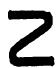
\includegraphics[keepaspectratio]{images/part001_b5dea1c7.jpg}}

在集合 \(\mathbf{R}^n\) 上，我们一方面要考虑它的（加法）拓扑群结构，另一方面要考虑它在域 \(\mathbf{R}\) 上的向量空间结构（第 VI 章 § 1 第 3 小节）。给定子集 \(\mathbf{A}\) （含于 \(\mathbf{R}^n\) ）后，我们可以考虑 \(\mathbf{R}^n\) 的由 \(\mathbf{A}\) 生成的子群（ \(\mathbf{A}\) 的点以整数为系数的一切线性组合所成的集合），同时也可以考虑由 \(\mathbf{A}\) 生成的向量子空间（ \(\mathbf{A}\) 的点以实数为系数的一切线性组合所成的集合）；必须仔细区分这两个概念。按照代数学中作出的定义， \(\mathbf{A}\) 的秩是向量子空间 \(\mathbf{V}\) （ \(\mathbf{R}^n\) 中由 \(\mathbf{A}\) 生成的）的维数；因此说 \(\mathbf{A}\) 的秩为 \(p\) ，就等价于说存在 \(p\) 个点 \(x_i \in \mathbf{A}\) ，它们关于域 \(\mathbf{R}\) 构成一个自由系（换句话说，关系 \(\sum_{i} t_i x_i = 0\) （其中 \(t_i\) 是实数）蕴涵 \(t_i = 0\) （对每个 \(i\) ）），并且构成 \(\mathbf{V}\) 的一个基（意即 \(\mathbf{V}\) 的每个点都是 \(x_i\) 以实数为系数的一个线性组合）。

在以下的内容中，我们还必须用到 \(\mathbf{R}^n\) 的点关于有理数域 \(\mathbf{Q}\) 自由这一概念；这样的系是一个有限子集 \((\pmb{x}_i)\) （ \(\mathbf{R}^n\) 的），满足关系 \(\sum_{i} r_i x_i = 0\) （其中 \(r_i\) 是有理数（或整数——这是一回事））蕴涵对每个 i 有 \(r_{i}=0\) 。这个概念必须与关于 R 的自由系的概念仔细地区分开：每个关于 R 自由的系都关于 Q 自由，但反过来不成立（例如，R 中的数 1 与 \(\sqrt{2}\) 构成关于 Q 的自由系，但不构成关于 R 的自由系）。每当我们不加限定地说到自由系时，总是指关于 R 的自由系。因此有必要在 \(R^{n}\) 上把关于 R 的向量空间结构与关于 Q 的向量空间结构区分开；特别地，由 \(R^{n}\) 的子集 A 生成的关于 Q 的向量子空间是 A 以有理数为系数的一切线性组合所成的集合 U；它含于由 A 生成的（关于 R 的）向量子空间 V，但一般与 V 不同。U（关于 Q）的维数称为 A 的有理秩；它至少等于上面定义的 A 的秩（即 V 关于 R 的维数）；若 A 是无限集，它可以是无限的，而 \(R^{n}\) 的任何非空子集的秩总 \(\leqslant n\) ；特别地， \(R^{n}\) 的任何不可数子集的有理秩总是无限的，因为 Q 上任何有限维向量空间都是可数的。

\pandocbounded{
\includegraphics[keepaspectratio]{images/part001_3371d17f.jpg}}

在本节中，我们将首先确定加法群 \(R^{n}\) 的闭子群的结构。

\subsection{\texorpdfstring{\(\mathbf{R}^n\) 的离散子群}{R 的 n 次幂的离散子群}}

我们在第 V 章（§ 1 第 1 小节命题 1）中已经看到，R 的闭子群中除 R 自身外只有离散子群，它们都由单个元素生成。我们将从考虑 \(\mathbf{R}^n\) 的离散子群开始。

首先，由 \(\mathbf{R}^n\) 的典范基（第 VI 章 § 1 第 3 小节）的 \(p\) 个向量（ \(p \leqslant n\) ）所生成的 \(\mathbf{R}^n\) 的子群是一个离散群，同构于乘积 \(\mathbf{Z}^p\) ——即 \(p\) 个都等于 \(\mathbf{Z}\) 的群的乘积。更一般地，考虑子群 \(\mathbf{G}\) ，它由构成自由系的 \(p\) 个点 \(a_i\) （ \(i \leqslant i \leqslant p\) ）生成。存在 \(\mathbf{R}^n\) 到其自身上的一个双射线性映射，它把 \(a_i\) 映为 \(e_i\) （ \(i \leqslant i \leqslant p\) ）；由于这样的映射是拓扑群 \(\mathbf{R}^n\) 的自同构， \(\mathbf{G}\) 作为拓扑群同构于由 \(e_i\) （ \(i \leqslant i \leqslant p\) ）生成的子群，因此是一个秩为 \(p\) 、同构于 \(\mathbf{Z}^p\) 的离散子群。

群 \(Z^{p}\) 的结构、从而 G 的结构，已在代数学中研究过。我们回顾这一研究的主要结果。G 关于环 Z 的基是由 p 个点组成的系

\[
\boldsymbol {b} _ {i} = \sum_ {j = 1} ^ {p} r _ {i j} \boldsymbol {a} _ {j},
\]

其中 \(r_{ij}\) 是使得行列式 \(\det(r_{ij})\) 等于 +1 或 -1 的整数。G 的每个子群 H 都是离散的且秩 \(q \leqslant p;\) 此外，若 \(H\) 是给定的秩为 \(q\) 的子群，则存在由 \(p\) 个点 \(b_i\) （ \(i \leqslant i \leqslant p\) ）组成并生成 \(G\) 的自由系，以及由 \(q\) 个点 \(c_i\) （ \(i \leqslant i \leqslant q\) ）组成并生成 \(H\) 的系，使得有 \(c_i = e_i b_i\) （对 \(i \leqslant i \leqslant q\) ），其中 \(e_i\) 是整数（ \(H\) 关于 \(G\) 的不变因子），满足

\[
e _ {i + 1} \equiv o (\mathrm{mod} e _ {i}) \quad \text { for } \quad i \leqslant i \leqslant q - i.
\]

商群 G/H 是一个离散群，同构于 \(Z^{p-q} \times F\) ，其中 F 是一个有限交换群，是 q 个循环子群的直积，这些循环子群的阶分别为 \(e_{1}, \ldots, e_{q}\) 。

现在我们将证明，刚才所考虑的 \(\mathbf{R}^n\) 的离散子群是仅有的离散子群。

命题 1. 设 G 是 \(\mathbf{R}^n\) 的一个秩为 \(p\) 的离散子群， \((\boldsymbol{a}_i)_{1 \leqslant i \leqslant p}\) 是 G 的 \(p\) 个点组成的自由系，P 是以 o 为中心、以 \(\boldsymbol{a}_i\) 为基向量的闭超平行体（第 VI 章 § 1 第 3 小节）。则集合 G ∩ P 是有限的且生成 G，且 G 的每个点都是 \(\boldsymbol{a}_i\) 以有理数为系数的线性组合。

G ∩ P 是紧的且离散的，因而是有限的。设 x 是 G 的任意点；它等于线性组合 \(\sum_{i=1}^{p} t_{i}a_{i}\) （诸 \(a_{i}\) 以实数为系数）。对每个整数 m \textgreater{} 0 ，考虑点

\[
z _ {m} = m x - \sum_ {i = 1} ^ {p} [ m t _ {i} ] a _ {i} = \sum_ {i = 1} ^ {p} (m t _ {i} - [ m t _ {i} ]) a _ {i} (*);
\]

它属于 G，且由于 \(o \leqslant mt_{i} - [mt_{i}] < 1\) ，它位于 P 中。因此，首先有 \(x = z_{1} + \sum_{i=1}^{p} [t_{i}] a_{i}\) ，故 G 由 \(G \cap P\) 生成；其次，由于 \(G \cap P\) 是有限的，存在两个不同的整数 h、k，使得 \(z_{h} = z_{k}\) ，从而 \((h - k)t_{i} = [ht_{i}] - [kt_{i}]\) （对 \((1 \leqslant i \leqslant p)\) ），因此 \(t_{i}\) 是有理数。

推论. 设 \((\pmb{a}_i)_{1\leqslant i\leqslant p}\) 是 \(p\) 个点（ \(\mathbf{R}^n\) 的）组成的自由系，并设

\[
\boldsymbol {b} = \sum_ {i = 1} ^ {p} t _ {i} \boldsymbol {a} _ {i}
\]

是 \(a_{i}\) 以实数为系数的一个线性组合。则 \(R^{n}\) 中由 \(p + i\) 个点 \(a_{1}, a_{2}, \ldots, a_{p}\) 与 b 所生成的子群 G 是离散的，当且仅当诸数 \(t_{i}\) 是有理数。

命题 1 表明这条件是必要的。它也是充分的，因为若这条件满足，我们就可以写 \(t_i = m_i / d\) ，其中 \(d\) 与诸 \(m_i\) 是整数（ \(i \leqslant i \leqslant p\) ）；于是 \(b\) 是 \(p\) 个点 ( \(\mathrm{I} / d\) ) \(a_i\) 以整数为系数的线性组合；因此 \(G\) 是由这 \(p\) 个点生成的离散群的一个子群，从而本身是离散的。

命题 1 的结果可以表述如下：若 q 个点 \(x_{i}\) （ \(i \leqslant i \leqslant q\) ，属于 \(R^{n}\) 的一个离散子群 G）构成一个关于 R 相关的系，则它们构成一个关于 Q 相关的系。由此立即推出， \(R^{n}\) 的离散子群的有理秩等于它的秩。

把命题 1 的推论应用到 \(a_{i}\) 为 \(n\) 个向量 \(\pmb{e}_{i}\) （ \(\mathbf{R}^{n}\) 的典范基的）的情形，就得到下面的命题：

命题 2（克罗内克）. 设 \(\theta_{1}, \theta_{2}, \ldots, \theta_{n}\) 是 \(n\) 个实数。为了对每个 \(\varepsilon > 0\) ，存在一个整数 \(q\) 与 \(n\) 个整数

\[
p _ {i} \quad (\mathrm{I} \leqslant i \leqslant n)
\]

使得

\[
\left| q \theta_ {i} - p _ {i} \right| \leqslant \varepsilon \quad (\mathrm{I} \leqslant i \leqslant n),
\]

其中这些不等式中至少有一个的左端不为零，其充分必要条件是诸 \(\theta_{i}\) 中至少有一个是无理数。

定理 1. \(\mathbf{R}^n\) 的每个秩等于 \(p\) 的离散子群 G 都由 \(p\) 个点组成的自由系生成。

根据前面回顾过的同构于 \(Z^{p}\) 的群的性质，只需证明 G 是由 p 个点组成的自由系生成的离散群的一个子群。现在，由于 G 的秩为 p，存在 G 的由 p 个点 \(a_{i}\) （ \(1 \leqslant i \leqslant p\) ）组成的自由系，使得每个 \(x \in G\)

都等于线性组合 \(\sum_{i=1}^{p} t_i a_i\) （诸 \(a_i\) 以实数为系数）；

由于 G 是离散的，命题 1 表明诸 \(t_i\) 是有理数。此外，命题 1 表明 G 由有限多个点生成；由于这些点是 \(\boldsymbol{a}_i\) 以有理数为系数的线性组合，故存在整数 \(d\) ，使得它们是 \(p\) 个点 \((\mathrm{I}/d)\boldsymbol{a}_i = \boldsymbol{a}_i'\) 以整数为系数的线性组合。由此推出，G 是由诸 \(\boldsymbol{a}_i'\) 生成的群的一个子群。

定理 1 也可以不用不变因子理论来证明（参见习题 1）。

\(R^{n}\) 中秩为 n 的离散子群也称为 \(R^{n}\) 中的格。

\subsection{\texorpdfstring{\(\mathbf{R}^n\) 的闭子群}{R 的 n 次幂的闭子群}}

我们已经知道 \(\mathbf{R}^n\) 的闭子群的两种类型：一方面是 \(\mathbf{R}^n\) 的向量子空间，它们同构于群 \(\mathbf{R}^p\) （ \(p \leqslant n\) ）（第 IV 章 § 1 第 4 小节命题 2）；另一方面是离散子群（第 III 章 § 2 第 1 小节命题 5），如我们刚才所见，它们同构于群 \(\mathbf{Z}^q\) （ \(q \leqslant n\) ）。现在我们要确定 \(\mathbf{R}^n\) 的任意闭子群的结构，办法是证明这样一个子群同构于形如

\[
\mathbf {R} ^ {p} \times \mathbf {Z} ^ {q} \quad \text { where } \quad \mathrm{o} \leqslant p + q \leqslant n.
\]

证明基于下面的命题：

命题 3. \(\mathbf{R}^n\) 的每个非离散的闭子群都包含一条过 o 的直线。

设 \((\pmb{x}_p)_{p\in \mathbb{N}}\) 是 \(\mathbf{G}\) 的点的一个无穷序列，满足 \(\pmb{x}_p\neq 0\) 且 \(\lim_{p\to \infty}\pmb{x}_p = 0\) ；由假设这样的序列存在。设 \(\mathbf{P}\) 是以 \(0\) 为中心且包含诸 \(\pmb{x}_p\) 的开立方体。设 \(k_{p}\) 表示最大的整数 \(h > 0\) ，它使 \(h\pmb{x}_p\in \mathrm{P}\) （由于 \(\mathbf{P}\) 是有界长方体且 \(\pmb{x}_p\neq 0\) ， \(k_{p}\) 的存在性由阿基米德公理得出）。点 \(k_{p}\pmb{x}_{p}\) 位于紧集 \(\overline{\mathrm{P}}\) 中，因此序列 \((k_{p}\pmb{x}_{p})_{p\in \mathbb{N}}\) 有一个聚点 \(\pmb {a}\in \overline{\mathrm{P}}\) 。若 \(||k_p\pmb {x}_p - \pmb {a}||\leqslant \varepsilon\) ，我们有

\[
\left| \left| \left(k _ {p} + \mathrm{I}\right) x _ {p} - a \right| \right| \leqslant \varepsilon + \left| \left| x _ {p} \right| \right|,
\]

且由于 \(\lim_{p\to \infty}\boldsymbol{x}_p = 0\) ，由此得出 \(\boldsymbol{a}\) 也是序列 \(((k_p + 1)x_p)\) 的一个聚点，而这个序列的点属于闭集 \(\mathfrak{C}P\) （按 \(k_{p}\) 的定义）；因此 \(\boldsymbol{a} \in \overline{\mathrm{P}} \cap \mathfrak{C}P\) （即 P 的边界，见图 5），这蕴涵 \(\boldsymbol{a} \neq 0\) 。此外，由于 G 是闭的，我们有 \(\boldsymbol{a} \in \mathrm{G}\) 。设 \(t\) 是任意实数；由于 \(|tk_p - [tk_p]| < 1\) ，关系 \(||k_p x_p - a|| \leqslant \varepsilon\) 蕴涵 \(||[tk_p]x_p - ta|| \leqslant |t| \varepsilon + ||x_p||\) ；由于 \(\lim_{p \to \infty} x_p = 0\) ， \(ta\) 是

\pandocbounded{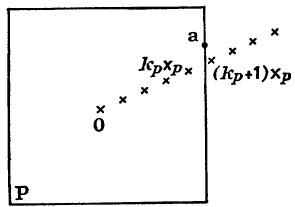
\includegraphics[keepaspectratio]{images/part001_2a0a1c84.jpg}}\\
图 5.

\pandocbounded{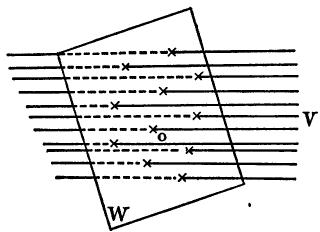
\includegraphics[keepaspectratio]{images/part001_3dc381fa.jpg}}\\
图 6.

序列 \(([tk_p]x_p)\) 的一个聚点；但这个序列的点都属于 G，因而 \(ta \in G\) ，因为 G 是闭的。证毕。

定理 2. 设 G 是 \(\mathbf{R}^n\) 的一个闭子群，其秩为 \(r\) （ \(0 \leqslant r \leqslant n\) ）。则存在含于 G 中的最大向量子空间 V；对每个与 V 互补的向量子空间 W，W ∩ G 是离散的，且 G 是 V 与 W ∩ G 的直和。

我们首先来确立 V 的存在性，办法是证明 G 中所有过 o 的直线的并集是一个向量子空间：事实上，由这些直线的并集生成的向量子空间与由它们生成的子群相同。群 G 是 V 与 W ∩ G 的直和；因为若 \(x \in G\) ，我们有 \(x = y + z\) ，其中 \(y \in V\) 且 \(z \in W\) ；由于 \(V \subset G\) ，有 \(z = x - y \in G\) ，因此 \(z \in W \cap G\) 。剩下要证明 \(W \cap G\) 是离散的；这由命题 3 得出，因为 \(W \cap G\) 是一个不含任何直线的闭子群，这是由 V 的定义推出的。

若 \(G \neq V\) ，我们可以说 G 是可数无穷多个线性簇的并，这些线性簇平行于 V 且经过离散群 \(W \cap G\) 的点（图 6）。

若 \(p\) 是向量子空间 \(\mathbf{V}\) 的维数，则 \(p \leqslant r\) ，且 \(\mathbf{W} \cap \mathbf{G}\) 是秩为 \(r - p\) 的离散群。

推论 1. 存在一个基 \((\pmb{a}_i)_{1\leqslant i\leqslant n}\) （ \(\mathbf{R}^n\) 的），使得

\[
\boldsymbol {a} _ {i} \in \mathrm{G} \quad (\mathrm{I} \leqslant i \leqslant r), \quad \boldsymbol {a} _ {i} \in \mathrm{V} \quad (\mathrm{I} \leqslant i \leqslant p)
\]

并且使得 \(\mathbf{G}\) 是形如 \(\sum_{i=1}^{p} t_i a_i + \sum_{j=p+1}^{r} n_j a_j\) 的点所成的集合，其中 \(t_i\) 取遍一切实数值，而 \(n_j\) 取遍一切整数值。

这由定理 2 以及应用于离散群 \(W \cap G\) 的第 1 小节的定理 1 得出。

推论 2. 存在 \(\mathbf{R}^n\) 的一个自同构，它把 \(\mathbf{G}\) 映到群 \(\mathbf{G}'\) 上，该群同构于 \(\mathbf{R}^p \times \mathbf{Z}^{r-p}\) ，是由 \(e_1, e_2, \ldots, e_p\) 生成的向量子空间与由 \(e_{p+1}, e_{p+2}, \ldots, e_r\) 生成的（离散）加法子群的直和。

这是推论 1 的直接推论。定理 2 的推论 2 表明， \(R^{n}\) 的闭子群 G 由两个 \(\geqslant 0\) 的整数完全确定（在相差一个同构的意义下）：它的秩，我们记作 \(r(\mathbf{G})\) ，以及含于 G 中的最大向量子空间的维数，我们称之为 G 的维数并记作 \(d(\mathbf{G})\) 。

这些整数需要满足的唯一条件是不等式 \(o \leqslant d(\mathbf{G}) \leqslant r(\mathbf{G}) \leqslant n\) 。

\subsection{相伴子群}

设 \(\mathbf{G}\) 是 \(\mathbf{R}^n\) 的任意子群（闭或不闭）。考虑集合 \(\mathbf{G}^*\) （由满足如下条件的点 \(\boldsymbol{u} = (u_i) \in \mathbf{R}^n\) 组成）：对一切 \(\boldsymbol{x} = (x_i) \in \mathbf{G}\) ，数 \((\boldsymbol{u}| \boldsymbol{x}) = \sum_{i=1}^{n} u_i x_i\) 是整数。立即可以看出， \(\mathbf{G}^*\) 是 \(\mathbf{R}^n\) 的一个子群；它称为与 \(\mathbf{G}(*)\) 相伴的子群。若 \(\mathbf{G}\) 与 \(\mathbf{H}\) 是 \(\mathbf{R}^n\) 的两个子群，且 \(\mathbf{H} \subset \mathbf{G}\) ，则显然有 \(\mathbf{G}^* \subset \mathbf{H}^*\) 。

命题 4. 子群 \(\mathbf{G}^*\) ——它与一个子群 \(\mathbf{G}\) （ \(\mathbf{R}^n\) 的）相伴——是闭的，且我们有 \((\overline{\mathbf{G}})^* = \mathbf{G}^*\) 。

对每个 \(x \in G\) ，用 \(f_x(u)\) 表示 \((u|x)\) ； \(f_x\) 是线性形式，因此是连续的。由于 \(G^*\) 是诸集合 \(f_x^{-1}(Z)\) （当 \(x\) 取遍 \(G\) 时）的交，且这些集合中的每一个都是闭的，由此得出 \(G^*\) 是闭的。另一方面，若 \(u \in G^*\) ，则有 \((u|x) \in Z\) （对一切 \(x \in G\) ），因而，由于 \(Z\) 在 \(R\) 中是闭的，有 \((u|y) \in Z\) （对一切 \(y \in \overline{G}\) ）；于是 \(u \in (G)^*\) 。但我们有 \((\overline{G})^* \subset G^*\) （因为 \(G \subset \overline{G}\) ），所以 \((\overline{G})^* = G^*\) 。

考虑 \(\mathbf{G}^*\) 在 \(\mathbf{G}\) 为闭时的结构。由第 2 小节定理 2 的推论 1，存在一个基 \((\pmb{a}_i)_{\mathbf{1} \leqslant i \leqslant n}\) （ \(\mathbf{R}^n\) 的），使得 \(\mathbf{G}\) 恰为由点

\[
\boldsymbol {x} = \sum_ {i = 1} ^ {p} t _ {i} \boldsymbol {a} _ {i} + \sum_ {j = p + 1} ^ {p + q} n _ {j} \boldsymbol {a} _ {j},
\]

所组成的集合，其中 \(t_i\) 取遍一切实数值，而 \(n_j\) 取遍一切整数值。于是 \((\boldsymbol{u}|\boldsymbol{x})\) 对所有这些点 \(\boldsymbol{x}\) 都是整数，当且仅当 \((\boldsymbol{u}|\boldsymbol{a}_i) = 0\) （对 \(1 \leqslant i \leqslant p\) ）且 \((\boldsymbol{u}|\boldsymbol{a}_i)\) 是整数（对 \(p + 1 \leqslant i \leqslant p + q\) ）。用 \((\boldsymbol{a}_i')_{1 \leqslant i \leqslant n}\) 表示 \(\mathbf{R}^n\) 的满足 \((\boldsymbol{a}_i'|\boldsymbol{a}_j) = 0\) （对 \(i \neq j\) ）的基

\[
\left(\boldsymbol {a} _ {i} ^ {\prime} \mid \boldsymbol {a} _ {i}\right) = \mathrm{I} \quad \text { for } \quad \mathrm{I} \leqslant i \leqslant n
\]

{[}即与 \((a_{i})\) “对偶”的基{]}；若置 \(u = \sum_{i=1}^{n} u_{i} a_{i}^{\prime}\) ，则显然点 \(u \in G^{*}\) 由下列条件刻画： \(u_{i} = 0\) （对 \(i \leqslant i \leqslant p\) ），且 \(u_{i} \in Z\) （对

\[
p + \mathrm{i} \leqslant i \leqslant p + q;
\]

因而 \(G^{*}\) 是一个向量子空间 W 与一个离散子群的直和，前者的基由那些 \(a_{i}^{\prime}\) （满足 \(p + q + i \leqslant i \leqslant n\) ）组成，后者由那些 \(a_{i}^{\prime}\) （满足 \(p + i \leqslant i \leqslant p + q\) ）生成。换言之：

命题 5. 对 \(\mathbf{R}^n\) 的每个闭子群 G ，

\[
r (\mathbf {G} ^ {*}) = n - d (\mathbf {G}) \quad a n d \quad d (\mathbf {G} ^ {*}) = n - r (\mathbf {G}).
\]

让我们把同样的推理应用于 \(\mathbf{G}^*\) 。注意到与 \((\pmb{a}_i')\) 对偶的基是 \((\pmb{a}_i)\) ，我们就看出：

命题 6. 对每个子群 \(\mathbf{G}\) （ \(\mathbf{R}^n\) 的），我们有 \((\mathbf{G}^*)^* = \overline{\mathbf{G}}\) 。

推论. 一点 x 位于 \(R^{n}\) 的子群 G 的闭包中，当且仅当 \((u|x)\) 对每个 \(u \in R^{n}\) 都是整数，其中 \((u|y)\) 对一切 \(y \in G\) 均为整数。

让我们把这个关于位于子群 \(\mathbf{G}\) 的闭包中的点的刻画，应用于子群 \(\mathbf{G}\) 的情形——它由 \(n\) 个向量 \(\boldsymbol{e}_j\) （ \(\mathrm{i} \leqslant j \leqslant n\) ，属于典范基）以及任意 \(m\) 个点 \(\boldsymbol{a}_i\) （ \(\mathrm{i} \leqslant i \leqslant m\) ，属于 \(\mathbf{R}^n\) ）生成。说 \((\boldsymbol{u}|\boldsymbol{e}_j)\) 对 \(\mathrm{i} \leqslant j \leqslant n\) 是整数，就意味着 \(n\) 个坐标（ \(\boldsymbol{u}\) 的）都是整数；因此：

命题 7（克罗内克）. 设 \(\boldsymbol{a}_i = (a_{ji})\) （ \(i \leqslant i \leqslant m\) ， \(i \leqslant j \leqslant n\) ）是 \(m\) 个点（ \(\mathbf{R}^n\) 的）， \(\boldsymbol{b} = (b_j)\) （ \(i \leqslant j \leqslant n\) ）是 \(\mathbf{R}^n\) 的一个点。为了对每个 \(\varepsilon > 0\) ，存在 \(m\) 个整数 \(g_i\) （ \(i \leqslant i \leqslant m\) ）与 \(n\) 个整数 \(p_j\) （ \(i \leqslant j \leqslant n\) ），使得

\[
\left| q _ {1} a _ {1 j} + q _ {2} a _ {2 j} + \dots + q _ {m} a _ {m j} - p _ {j} - b _ {j} \right| \leqslant \varepsilon \quad (\mathrm{I} \leqslant j \leqslant n)
\]

其必要充分条件是：对每个有限序列 \((r_j)\) （ \(1 \leqslant j \leqslant n\) ，由 \(n\) 个整数组成），只要 \(m\) 个数 \(\sum_{j=1}^{n} a_{ij} r_j\) （ \(1 \leqslant i \leqslant m\) ）都是整数，数 \(\sum_{j=1}^{n} b_j r_j\) 就也是整数。

推论 1. 为了对每个 \(\boldsymbol{x} = (x_{j}) (\mathrm{I} \leqslant j \leqslant n)\) 与每个 \(\varepsilon > 0\) ，存在 m 个整数 \(q_{i} (\mathrm{I} \leqslant i \leqslant m)\) 与 n 个整数

\(p_j\) (1 \(\leqslant j\leqslant n\) )，使得

\[
\left| q _ {1} a _ {1 j} + q _ {2} a _ {2 j} + \dots + q _ {m} a _ {m j} - p _ {j} - x _ {j} \right| \leqslant \varepsilon \quad (\mathrm{I} \leqslant j \leqslant n)
\]

其必要充分条件是：不存在有限序列 \((r_j)\) （由 \(n\) 个整数组成、不全为零），使得 \(m\) 个数 \(\sum_{j=1}^{n} a_{ij} r_j\) 中的每一个都是整数。因为若 \(G\) 在 \(\mathbf{R}^n\) 中稠密，即若 \(\overline{\mathbf{G}} = \mathbf{R}^n\) ，则 \(\mathbf{G}^* = \{o\}\) ，反之亦然。

特别地 \((m = \mathrm{i})\) ：

推论 2. 设 \(\theta_{1},\theta_{2},\ldots ,\theta_{n}\) 是 \(n\) 个实数。为了对给定的任意 \(n\) 个实数 \(x_{1},x_{2},\ldots ,x_{n}\) 以及一个实数 \(\varepsilon >0\) ，存在一个整数 \(q\) 与 \(n\) 个整数 \(p_j\) ，使得

\[
\left| q \theta_ {j} - p _ {j} - x _ {j} \right| \leqslant \varepsilon \quad (\mathrm{I} \leqslant j \leqslant n)
\]

其必要充分条件是：不存在形如 \(\sum_{j=1}^{n} r_j \theta_j = h\) 的关系，其中 \(r_j\) 是 \(n\) 个不全为零的整数，而 \(h\) 是整数{[}这特别蕴涵诸 \(\theta_j\) 以及诸比 \(\theta_j / \theta_k\) （ \(j \neq k\) ）都必须是无理数{]}。

我们可以把这个结果解释如下：对每个整数 \(q \in Z\) ，设 \(x_{q}\) 是以 \(q\theta_{j} - [q\theta_{j}]\) （ \(i \leqslant j \leqslant n\) ）为坐标的点；于是推论 2 给出了使点 \(x_{q}\) 所成的集合在立方体（即区间 {[}0, i{]} ——在 \(R^{n}\) 的诸因子中——的乘积）中稠密的一个必要充分条件。

命题 8. 若 \(G_{1}\) 、 \(G_{2}\) 是 \(R^{n}\) 的任意闭子群，则我们有

\[
(\mathrm{G} _ {1} + \mathrm{G} _ {2}) ^ {*} = \mathrm{G} _ {1} ^ {*} \cap \mathrm{G} _ {2} ^ {*} \quad a n d \quad (\mathrm{G} _ {1} \cap \mathrm{G} _ {2}) ^ {*} = \mathrm{G} _ {1} ^ {*} + \mathrm{G} _ {2} ^ {*}.
\]

实数 \((\pmb{u}|\pmb{x} + \pmb{y})\) 对一切 \(\pmb{x} \in \mathbf{G}_1\) 与一切 \(\pmb{y} \in \mathbf{G}_2\) 都是整数，当且仅当 \((\pmb{u}|\pmb{x})\) 对一切 \(\pmb{x} \in \mathbf{G}_1\) 是整数且 \((\pmb{u}|\pmb{y})\) 对一切 \(\pmb{y} \in \mathbf{G}_2\) 是整数，因为 \((\pmb{u}|\pmb{x} + \pmb{y}) = (\pmb{u}|\pmb{x}) + (\pmb{u}|\pmb{y})\) ；因此

\[
(\mathrm{G} _ {1} + \mathrm{G} _ {2}) ^ {*} = \mathrm{G} _ {1} ^ {*} \cap \mathrm{G} _ {2} ^ {*}
\]

对任意两个子群 \(G_{1}\) 、 \(G_{2}\) （ \(R^{n}\) 的）成立。现在若假设 \(G_{1}\) 与 \(G_{2}\) 是闭的，则由命题 6 有 \((\mathbf{G}_{1}^{*} + \mathbf{G}_{2}^{*})^{*} = \mathbf{G}_{1} \cap \mathbf{G}_{2}\) ；因此，取相伴子群并再次应用命题 6，就得到 \((\mathbf{G}_{1} \cap \mathbf{G}_{2})^{*} = \overline{\mathbf{G}_{1}^{*} + \mathbf{G}_{2}^{*}}\) 。

注. 设 \(\mathbf{G}_1, \mathbf{G}_2\) 是 \(\mathbf{R}^n\) 中（第 1 小节意义下）的两个格，且 \(\mathbf{G}_2 \subset \mathbf{G}_1\) ；则（命题 5） \(\mathbf{G}_1^*\) 与 \(\mathbf{G}_2^*\) 是 \(\mathbf{R}^n\) 中满足 \(\mathbf{G}_1^* \subset \mathbf{G}_2^*\) 的格。我们在第 1 小节中已经看到，存在整数 \(m > 0\) 使 \(m\mathbf{G}_1 \subset \mathbf{G}_2\) ；

因而对 \(x \in G_1\) 与 \(u \in G_2^*\) ，我们有 \(m(u|x) \in Z\) ，从而 \((u|x) \in Q\) 。若 \(x \in G_2\) 且 \(u \in G_2^*\) ，或者 \(x \in G_1\) 且 \(u \in G_1^*\) ，则按定义有 \((u|x) \in Z\) 。于是，过渡到商后， \(Z\) -双线性映射 \((x, u) \to (u|x)\) （ \(G_1 \times G_2^*\) 到 \(Q\) 中的）定义了 \(Z\) -双线性映射 \(B\) （ \((G_1/G_2) \times (G_2^*/G_1^*)\) 到 \(Q/Z\) 中的）。此外，显然若 \(\bar{x}_0 \in G_1/G_2\) （相应地， \(\bar{u}_0 \in G_2^*/G_1^*\) ）使得对每个 \(\bar{u} \in G_2^*/G_1^*\) （相应地，对每个 \(\bar{x} \in G_1/G_2\) ）我们有

\[
\mathrm{B} (\overline {{{\boldsymbol {x}}}} _ {0}, \boldsymbol {u}) = \mathrm{o} \quad [ \text { resp. } \mathrm{B} (\overline {{{\boldsymbol {x}}}}, \overline {{{\boldsymbol {u}}}} _ {0}) = \mathrm{o} ],
\]

则必有 \(\overline{\mathbf{x}}_0 = \mathbf{o}\) （相应地， \(\overline{\mathbf{u}}_0 = \mathbf{o}\) ）。由此得出，存在一个 \(\mathbf{Z}\) -线性双射 \(h\) （ \(\mathrm{G}_2^* / \mathrm{G}_1^*\) 到 \(\mathrm{G}_1 / \mathrm{G}_2\) 的对偶上的），使得 \(\langle \overline{\mathbf{x}}, h(\overline{\mathbf{u}}) \rangle = \mathrm{B}(\overline{\mathbf{x}}, \overline{\mathbf{u}})\) （对 \(\overline{\mathbf{x}} \in \mathrm{G}_1 / \mathrm{G}_2\) 与 \(\overline{\mathbf{u}} \in \mathrm{G}_2^* / \mathrm{G}_1^*\) ）；特别地，有限群 \(\mathrm{G}_1 / \mathrm{G}_2\) 与 \(\mathrm{G}_2^* / \mathrm{G}_1^*\) 是同构的。

\subsection{\texorpdfstring{\(R^{n}\) 的豪斯多夫商群}{R 的 n 次幂的豪斯多夫商群}}

\(\mathbf{R}^n\) 的每个豪斯多夫商群都形如 \(\mathbf{R}^n/\mathbf{H}\) ，其中 \(\mathbf{H}\) 是 \(\mathbf{R}^n\) 的闭子群（第 III 章 § 2 第 6 小节命题 18）。由第 3 小节定理 2 的推论 2，存在一个自同构 \(f\) （ \(\mathbf{R}^n\) 的），它把 \(\mathbf{H}\) 变成子群 \(\mathbf{H}'\) ，即由 \(p\) 个向量 \(\boldsymbol{e}_i\) （典范基的）所生成的向量子空间与由 \(q\) 个其余向量（共 \(n-p\) 个）所生成的离散群的直和

\[
\boldsymbol {e} _ {i}, \quad \mathrm{o} \leqslant p + q \leqslant n.
\]

过渡到商后， \(f\) 诱导出 \(\mathbf{R}^n / \mathbf{H}\) 到 \(\mathbf{R}^n / \mathbf{H}'\) 上的一个同构（第 III 章 § 2 第 8 小节注 3）；而 \(\mathbf{R}^n / \mathbf{H}'\) 同构于 \(\mathbf{R}^{n - p - q} \times \mathbf{T}^q\) （第 III 章 § 2 第 9 小节命题 26 的推论）。因此：

命题 9. \(\mathbf{R}^{n}\) 的每个豪斯多夫商群都同构于一个乘积群 \(\mathbf{R}^{h} \times \mathbf{T}^{k}\) （ \(0 \leqslant h + k \leqslant n\) ）。

乘积空间 \(\mathbf{T}^n\) （并且，沿用习惯的说法，拓扑群 \(\mathbf{T}^n\) ）称为 \(n\) 维环面；由第 V 章 § 1 第 2 小节命题 4， \(\mathbf{T}^n\) 是紧的、连通的且局部连通的。

此外，若用 C 表示 \(R^{n}\) 中边长为 1 的闭立方体，则 \(T^{n}\) 同胚于 C 关于等价关系`` \(x_{i} \equiv y_{i} \pmod{1}\) （ \(1 \leqslant i \leqslant n\) ）''（在 C 的点 \(\boldsymbol{x} = (\boldsymbol{x}_{i})\) 与 \(\boldsymbol{y} = (\boldsymbol{y}_{i})\) 之间）的商空间。于是 \(T^{n}\) 是由立方体 C 经过“把相对的面粘合起来”而得到的。

命题 10. 拓扑群 \(\mathbf{T}^n\) 局部同构于 \(\mathbf{R}^n\) 。因为 \(\mathbf{T}^n = (\mathbf{R}/\mathbf{Z})^n\) 同构于 \(\mathbf{R}^n/\mathbf{Z}^n\) （第 III 章 § 2 第 9 小节命题 26 的推论），而 \(\mathbf{Z}^n\) 是 \(\mathbf{R}^n\) 的离散子群（第 III 章 § 2 第 6 小节命题 19）。

由此得出，诸群 \(\mathbf{R}^p\times \mathbf{T}^{n - p}\) 都局部同构于 \(\mathbf{R}^n\) \((\mathrm{o}\leqslant p\leqslant n)\) ；在 § 2 第 2 小节中我们将看到，它们是具有此性质的仅有的连通群。

\subsection{\texorpdfstring{\(T^{n}\) 的子群与商群}{T 的 n 次幂的子群与商群}}

让我们把 \(\mathbf{T}^n\) 与 \(\mathbf{R}^n/\mathbf{Z}^n\) 等同起来，并设 \(\varphi\) 是 \(\mathbf{R}^n\) 到 \(\mathbf{R}^n/\mathbf{Z}^n\) 上的典范同态。 \(\mathbf{T}^n\) 的每个子群都形如 \(\mathbf{G} = \varphi(\mathbf{H})\) ，其中 \(\mathbf{H}\) 是 \(\mathbf{R}^n\) 的包含 \(\mathbf{Z}^n\) 的子群，且它同构于 \(\mathbf{H}/\mathbf{Z}^n\) （第 III 章 § 2 第 7 小节命题 20）； \(\mathbf{G}\) 在 \(\mathbf{T}^n\) 中为闭的必要充分条件是 \(\mathbf{H}\) 在 \(\mathbf{R}^n\) 中为闭（第 I 章 § 3 第 4 小节）。于是，为了求出 \(\mathbf{T}^n\) 的闭子群，我们必须确定一切闭子群 \(\mathbf{H}\) （ \(\mathbf{R}^n\) 的，包含 \(\mathbf{Z}^n\) ）；为此我们将利用第 3 小节的命题 6，并且先来确定子群 \(\mathbf{H}^*\) （与 \(\mathbf{H}\) 相伴的）。由于 \(\mathbf{Z}^n\) 与其自身相伴，我们有 \(\mathbf{H}^* \subset \mathbf{Z}^n\) ；因而（第 1 小节）存在基 \((\boldsymbol{a}_i)_{1 \leqslant i \leqslant n}\) （ \(\mathbf{R}^n\) 的，它生成 \(\mathbf{Z}^n\) ），以及 \(\mathbf{H}^*\) 的（关于环 \(\mathbf{Z}\) 的）由 \(p\) 个点 \(\boldsymbol{b}_i\) （ \(1 \leqslant i \leqslant p\) ）组成的基，使得 \(\boldsymbol{b}_i = e_i \boldsymbol{a}_i\) （ \(1 \leqslant i \leqslant p\) ），其中诸 \(e_i\) 是满足同余关系 \(e_{i+1} \equiv o (\text{mod } e_i)\) （对 \(1 \leqslant i \leqslant p - 1\) ）的整数。设 \((\boldsymbol{a}_i')\) 是与 \((\boldsymbol{a}_i)\) 对偶的基；则 \(\boldsymbol{u} = \sum_{i=1}^{n} u_i \boldsymbol{a}_i'\) 属于 \((\mathrm{H}^*)^* = \mathrm{H}\) ，当且仅当 \(u_i e_i \in \mathbf{Z}\) （对 \(1 \leqslant i \leqslant p\) ）；换言之， \(\mathbf{H}\) 是由 \(\boldsymbol{a}_{p+1}'\) ， \ldots, \(\boldsymbol{a}_n'\) 所生成的向量子空间 V 与由 \(p\) 个点

\[
e _ {i} ^ {- 1} \boldsymbol {a} _ {i} ^ {\prime} \quad (\mathrm{I} \leqslant i \leqslant p).
\]

另一方面， \(\mathbf{Z}^n\) 是 \(\mathbf{V} \cap \mathbf{Z}^n\) 与 \(\mathbf{K} \cap \mathbf{Z}^n\) 的直和，因为诸 \(a_i'\) （ \(i \leqslant i \leqslant n\) ）生成 \(\mathbf{Z}^n\) 。于是商群 \(\mathrm{H} / \mathbf{Z}^n\) 同构于 \((\mathrm{V} / (\mathrm{V} \cap \mathbf{Z}^n)) \times (\mathrm{K} / (\mathrm{K} \cap \mathbf{Z}^n))\) （第 III 章 § 2 第 9 小节命题 26 的推论）； \(\mathrm{V} / (\mathrm{V} \cap \mathbf{Z}^n)\) 同构于 \(\mathbf{T}^{n-p}\) ，而 \(\mathbf{K} / (\mathbf{K} \cap \mathbf{Z}^n)\) 是一个有限群，是 \(p\) 个循环群的直和，这些循环群的阶分别为 \(e_i\) （ \(i \leqslant i \leqslant p\) ）（参见第 1 小节）。

沿用同样的记号， \(T^{n}\) 的每个豪斯多夫商群都形如 \(\mathbf{T}^{n}/\varphi(\mathbf{H})\) ，且同构于 \(R^{n}/H\) （第 III 章 § 2 第 7 小节命题 22 的推论）；若 W 是由 K 生成的向量子空间，则 \(R^{n}/H\) 同构于 W/K（第 III 章 § 2 第 9 小节命题 26 的推论），即同构于 \(T^{p}\) 。综上所述：

命题 11. \(\mathbf{T}^n\) 的每个闭子群都同构于形如 \(\mathbf{T}^h \times \mathbf{F}\) 的群（ \(0 \leqslant h \leqslant n\) ），其中 \(\mathbf{F}\) 是一个有限交换群，且使得 \(\mathbf{F}\) 是其直和的循环子群的最小个数 \(\leqslant n - h\) 。 \(\mathbf{T}^n\) 的每个豪斯多夫商群都同构于形如 \(\mathbf{T}^h\) 的群（ \(0 \leqslant h \leqslant n\) ）。

特别地 \((n = 1)\) ：

推论. T 的每个闭子群，除 T 自身外，都是有限循环群。T 的每个豪斯多夫商群，除 \(\{o\}\) 外，都同构于 T。

\subsection{周期函数}

定义 1. 函数 \(f\) （定义在 \(\mathbf{R}^n\) 上、取值于任意集合 \(\mathbf{E}\) 中的）称为周期的，如果存在一点 \(a \neq 0\) （ \(\mathbf{R}^n\) 中的），使得

\[
f (\boldsymbol {x} + \boldsymbol {a}) = f (\boldsymbol {x})\tag{1}
\]

对一切 \(x \in R^{n}\) 成立。若 f 是周期的，则使关系 (1) 成为关于 x 的恒等式的每个点 \(a \in R^{n}\) 都称为 f 的一个周期。

周期函数 f 的所有周期所成的集合 G 显然是加法群 \(R^{n}\) 的一个子群（由假设它不只由 o 组成）。若 f 是 \(R^{n}\) 到豪斯多夫拓扑空间 E 中的连续周期映射，则它的周期群 G 是闭的。因为若用 \(G_{x}\) 表示由一切 \(a \in R^{n}\) （使得 \(f(x + a) = f(x)\) ，对给定的点 \(x \in R^{n}\) ）组成的集合，则 G 是诸 \(G_{x}\) （当 x 取遍 \(R^{n}\) 时）的交，而每个 \(G_{x}\) 都是闭的（第 I 章 § 8 第 1 小节命题 2）。设 V 是含于 G 中的最大向量子空间（第 2 小节定理 2）；函数 f 在模 V 的每个陪集上都取常值；若 W 是与 V 互补的向量子空间，则 f 由它在 W 上的限制确定。换言之（W 是同构于某个 \(R^{p}\) 的拓扑群，p 是某个整数）， \(R^{n}\) 上连续周期函数的研究可归结为这类函数中周期群 G 为离散群者的研究；若这个群的秩为 q，则称函数 f 是 q 重周期的，而生成 G 的 q 个点的每个自由系都称为 f 的一个基本周期系。

若 \((\boldsymbol{a}_{i})\) 与 \((\boldsymbol{b}_{i})\) 是 f 的两个基本周期系，则我们已看到（第 1 小节），每个都可以由另一个通过一个以整数为系数、行列式为 \(\pm1\) 的线性变换得到。

设 \(\varphi\) 是 \(\mathbf{R}^n\) 到 \(\mathbf{R}^n/\mathbf{G}\) 上的典范映射；对每个映射 \(g\) （ \(\mathbf{R}^n/\mathbf{G}\) 到集合 \(\mathbf{E}\) 中的），对应着函数 \(\dot{g}=g\circ\varphi\) ，它是 \(\mathbf{R}^n\) 到 \(\mathbf{E}\) 中的周期映射，其周期群包含 G；反过来，每个周期群包含 G 的 \(R^{n}\) 到 E 中的映射都具有这种形式，因为它与关系 \(x \equiv y \pmod{G}\) 相容（《集合论》R， § 5 第 7 小节）。这样我们就定义了一个双射 \(g \to \dot{g}\) ，它把 \(R^{n}/G\) 到 E 中的一切映射所成的集合映到 \(R^{n}\) 到 E 中且周期群包含 G 的一切映射所成的集合上。为使 \(\dot{g}\) 连续（E 是拓扑空间），必要充分条件是 g 连续（第 I 章 § 3 第 4 小节命题 6）。

\section{\texorpdfstring{\(\mathbf{R}^n\) 及其商群的连续同态}{R 的 n 次幂及其商群的连续同态}}

\subsection{\texorpdfstring{群 \(R^{m}\) 到群 \(R^{n}\) 中的连续同态}{群 R 的 m 次幂到群 R 的 n 次幂中的连续同态}}

\(\mathbf{R}^{m}\) 到 \(\mathbf{R}^{n}\) 中的每个线性映射（参见第 VI 章 § 1 第 3 小节）显然都是加法群 \(\mathbf{R}^{m}\) 到加法群 \(\mathbf{R}^{n}\) 中的连续同态。反过来：

命题 1. 每个连续同态 \(f\) （加法群 \(\mathbf{R}^m\) 到加法群 \(\mathbf{R}^n\) 中的）都是 \(\mathbf{R}^m\) 到 \(\mathbf{R}^n\) 中的线性映射。

只需证明 \(f(tx) = tf(x)\) 对一切 \(x \in \mathbf{R}^n\) 与一切 \(t \in \mathbf{R}\) 成立。其论证与第 V 章 § 1 第 3 小节命题 5 的相同，只要把 \(x\) 换成 \(x\) 、把 \(\mathbf{R}\) 换成 \(\mathbf{R}^m\) 。

\subsection{\texorpdfstring{\(R^{n}\) 到拓扑群中的连续同态的局部定义}{R 的 n 次幂到拓扑群中的连续同态的局部定义}}

第 V 章 § 1 第 4 小节的命题 6 可以推广到所有的群 \(\mathbf{R}^n\) 。

命题 2. 设 A 是 \(\mathbf{R}^n\) 中包含 o 的一个超平行体；设 \(f\) 是 A 到拓扑群 G（写成乘法）中的连续映射，使得 \(f(x + y) = f(x)f(y)\) 对每对点 \(x, y\) （满足 \(x \in A\) 、 \(y \in A\) 与 \(x + y \in A\) ）成立。则存在 \(\mathbf{R}^n\) 到 G 中的唯一连续同态，它延拓 \(f\) 。

用第 V 章 § 1 第 4 小节命题 6 中的同样论证可以证明：延拓 \(f\) 的同态如果存在，则是唯一的。其次，子群 \(G_1\) （ \(G\) 的，由 \(f(A)\) 生成）是交换的；因为若 \(x\) 与 y 是 A 的任意两点，则 \(\frac{1}{2}x\) 、 \(\frac{1}{2}y\) 与 \(\frac{1}{2}(x+y)\) 都属于 A，因此

\[
f \left(\frac {1}{2} (\boldsymbol {x} + \boldsymbol {y})\right) = f \left(\frac {1}{2} \boldsymbol {x}\right) f \left(\frac {1}{2} \boldsymbol {y}\right) = f \left(\frac {1}{2} \boldsymbol {y}\right) f \left(\frac {1}{2} \boldsymbol {x}\right),
\]

这表明 \(f(\frac{1}{2} x)\) 与 \(f(\frac{1}{2} y)\) 交换；因此 \(f(x) = (f(\frac{1}{2} x))^2\) 与 \(f(y) = (f(\frac{1}{2} y))^2\) 也交换，这就证明了断言。

设 \(a_1, a_2, \ldots, a_n\) 是 \(n\) 个非零向量（含于 \(A\) 中且与超平行体的基向量成比例），且对每个指标 \(i\) ，设 \(D_i\) 是过 \(o\) 与 \(a_i\) 的直线，即诸点 \(ta_i\) （当 \(t\) 取遍 \(R\) 时）所成的集合。设 \(A_i\) 是一切 \(t \in R\) （使 \(ta_i \in A\) ）所成的集合；则 \(A_i\) 是 \(R\) 的一个包含 \([o, i]\) 的区间，而函数

\[
f _ {i} (t) = f \left(t \boldsymbol {a} _ {i}\right)
\]

在 \(A_{i}\) 上有定义且连续，并满足关系

\[
f _ {i} (t + t ^ {\prime}) = f _ {i} (t) f _ {i} (t ^ {\prime})
\]

只要 \(t, t'\) 与 \(t + t'\) 都属于 \(A_i\) 。由第 V 章 § 1 第 4 小节命题 6，存在一个连续同态 \(\overline{f}_i\) （ \(\mathbf{R}\) 到 \(G\) 中的），它延拓 \(f_i\) 。由于 \(\mathbf{R}^n\) 是诸子群 \(D_i\) 的直和，我们可以定义一个同态 \(\overline{f}\) （ \(\mathbf{R}^n\) 到交换群 \(G_1\) 中的），其规则为 \(\overline{f}(x) = \prod_{i=1}^{n} \overline{f}_i(t_i)\) （其中 \(x = \sum_{i=1}^{n} t_i a_i\) ）； \(\overline{f}\) 是 \(f\) 的延拓，因为若 \(x \in A\) ，则诸分量 \(x_i\) （ \(x\) 在诸直线 \(D_i\) 上的）也都属于 \(A\) （由诸 \(a_i\) 的取法）；此外， \(\overline{f}\) 在 \(R^n\) 上连续，因为它在每条直线 \(D_i\) 上连续，且 \(x_i\) 是 \(x\) 的线性函数（因而连续）。

推论 1. 设 V 是 \(R^{n}\) 中 o 的一个邻域，f 是 V 到拓扑群 G 中的连续映射，使得

\[
f (\boldsymbol {x} + \boldsymbol {y}) = f (\boldsymbol {x}) f (\boldsymbol {y})
\]

对每对点 \(x, y\) （满足 \(x \in V\) 、 \(y \in V\) 与 \(x + y \in V\) ）成立。则存在 \(\mathbf{R}^n\) 到 \(G\) 中的唯一连续同态，它与 \(f\) 在一个邻域 \(W\) （ \(o\) 的）的所有点处一致。

取 W 为以 o 为中心、含于 V 中的开长方体，并对 W 应用命题 2。

我们以后将看到， \(R^{n}\) 的这个性质可以推广到更大的一类拓扑群，即“单连通”群。

推论 2. 设 \(f\) 是 \(\mathbf{R}^n\) 与拓扑群 \(\mathbf{G}\) 之间的一个局部同构。则存在 \(\mathbf{R}^n\) 到 \(\mathbf{G}\) 的一个开子群上的唯一严格态射，它与 \(f\) 在 \(\mathbf{o}\) 的某个邻域的所有点处一致。

设 \(\overline{f}\) 是 \(\mathbf{R}^n\) 到 \(\mathbf{G}\) 中的、在 o 的某个邻域的所有点处与 \(f\) 一致的连续同态；由假设， \(\overline{f}(\mathbf{R}^n)\) 包含 \(\mathbf{G}\) 的单位元的一个邻域，因此（第 III 章 § 2 第 1 小节命题 4 的推论）是 \(\mathbf{G}\) 的一个开子群；此外，由第 III 章 § 2 第 8 小节命题 24， \(\overline{f}\) 是 \(\mathbf{R}^n\) 到 \(\overline{f}(\mathbf{R}^n)\) 上的一个严格态射。

定理 1. 每个局部同构于 \(\mathbf{R}^n\) 的连通群 G 都同构于某个群 \(\mathbf{R}^p \times \mathbf{T}^{n-p}\) （ \(0 \leqslant p \leqslant n\) ）。

适当选取的局部同构 \(f\) （在 \(\mathbf{R}^n\) 与 \(G\) 之间）可以延拓为 \(\mathbf{R}^n\) 到 \(G\) 的一个开子群上的严格态射（命题 2 的推论 2），并由于 \(G\) 连通而延拓到 \(G\) 自身。由此得出 \(G\) 同构于一个商群 \(\mathbf{R}^n / H\) （ \(\mathbf{R}^n\) 的）： \(H\) 是离散的，否则会存在点 \(x \neq 0\) （属于 \(H\) ，且任意接近 \(o\) ）使得 \(f(x) = f(0)\) ，这与 \(f\) 是局部同构这一假设相矛盾。因此定理是 § 1 第 1 小节定理 1 的推论。

\subsection{\texorpdfstring{\(R^{m}\) 到 \(T^{n}\) 中的连续同态}{R 的 m 次幂到 T 的 n 次幂中的连续同态}}

命题 3. \(\mathbf{R}^m\) 到 \(\mathbf{T}^n\) 中的每个连续同态都形如 \(x \to \varphi(u(x))\) ，其中 \(\varphi\) 是 \(\mathbf{R}^n\) 到 \(\mathbf{T}^n\) （与 \(\mathbf{R}^n / \mathbf{Z}^n\) 等同）上的典范同态，而 \(u\) 是 \(\mathbf{R}^m\) 到 \(\mathbf{R}^n\) 中的线性映射。

设 \(f\) 是 \(\mathbf{R}^m\) 到 \(\mathbf{T}^n\) 中的一个连续同态。我们将证明，存在线性映射 \(u\) （ \(\mathbf{R}^m\) 到 \(\mathbf{R}^n\) 中的），使得同态 \(x \to f(x)\) 与 \(x \to \varphi(u(x))\) 在 \(o\) 于 \(\mathbf{R}^m\) 中的一个邻域的所有点处一致；于是命题由第 2 小节命题 2 的推论 1 得出。现在设 \(V\) 是 \(o\) 于 \(\mathbf{R}^n\) 中的一个这样的邻域： \(\varphi\) 在 \(V\) 上的限制是 \(\mathbf{R}^n\) 与 \(T^n\) 之间的一个局部同构，并设 \(\psi\) 是 \(\varphi\) 的逆映射，定义在 \(\varphi(V)\) 上。由于 \(f\) 连续， \(V' = \overline{f}^{-1}(\varphi(V))\) 是 \(o\) 于 \(\mathbf{R}^m\) 中的一个邻域；映射

\[
\boldsymbol {x} \rightarrow \psi (f (\boldsymbol {x})),
\]

限制在 \(V'\) 上，是 \(V'\) 到 \(R^n\) 中的连续映射，使得 \(\psi(f(x+y)) = \psi(f(x)) + \psi(f(y))\) 对 \(R^m\) 中每对满足 \(x \in V'\) 、 \(y \in V'\) 与 \(x + y \in V'\) 的点 x、y 成立；因而（第 2 小节命题 2 的推论 1）这个映射与一个完全确定的 \(R^m\) 到 \(R^n\) 中的连续同态 u 在 \(\mathbf{R}^m\) 中 o 的一个邻域 W 的所有点处一致。由命题 1（第 1 小节）， \(u\) 是 \(\mathbf{R}^m\) 到 \(\mathbf{R}^n\) 中的线性映射；于是对一切 \(x \in W\) 有 \(f(x) = \varphi(u(x))\) ，证明完毕。

注. 同样的论证更一般地表明：若 \(\varphi\) 是 \(R^{n}\) 到群 G 中的严格态射，它在 o 的适当邻域上的限制是 \(R^{n}\) 与 G 之间的局部同构，则 \(R^{n}\) 到 G 中的每个连续同态都形如 \(x \to \varphi(u(x))\) ，其中 u 是 \(R^{m}\) 到 \(R^{n}\) 中的线性映射。

在 \(m = n = 1\) 的情形，命题 3 给出：

命题 4. 若 \(\varphi\) 是 \(\mathbf{R}\) 到 \(\mathbf{T}\) 上的典范同态，则 \(\mathbf{R}\) 到 \(\mathbf{T}\) 中的每个连续同态都形如 \(x \to \varphi(ax)\) ，其中 \(a \in \mathbf{R}\) ；且它是 \(\mathbf{R}\) 到 \(\mathbf{T}\) 上的严格态射（当 \(a \neq 0\) 时）。

\subsection{\texorpdfstring{\(\mathbf{T}^n\) 的自同构}{T 的 n 次幂的自同构}}

设 H 是 \(R^{n}\) 的闭子群， \(\varphi\) 是 \(R^{n}\) 到商群 \(R^{n}/H\) 上的典范同态。若 f 是 \(R^{n}/H\) 到拓扑群 G 中的连续同态，则 \(\dot{f} = f \circ \varphi\) 是 \(R^{n}\) 到 G 中的连续同态，它是周期的，且其周期群包含 H；反过来，每个周期群包含 H 的 \(R^{n}\) 到 G 中的周期连续同态都具有这种形式。

在 \(H = Z^{n}\) 的情形，商群 \(R^{n}/Z^{n} = T^{n}\) 是紧的，因此只要 G 是豪斯多夫的， \(T^{n}\) 到拓扑群 G 中的每个连续同态 f 都是 \(T^{n}\) 到 G 中的严格态射（第 III 章 § 2 第 8 小节注 1）； \(\dot{f} = f \circ \varphi\) 是 \(R^{n}\) 到 G 中的严格态射；此外， \(f(\mathbf{T}^{n}) = \dot{f}(\mathbf{R}^{n})\) 是 G 的一个紧子群，同构于某个群 \(T^{p}\) （ \(o \leqslant p \leqslant n\) ）。

特别地，我们看到 \(T^{n}\) 到群 \(R^{m}\) 中的连续同态只有零映射，因为 \(\{0\}\) 是 \(R^{m}\) 的唯一紧子群。

让我们把这个应用于 \(\mathbf{T}^n\) 到群 \(\mathbf{T}^p\) 中的连续同态；若 \(f\) 是这样一个同态， \(\varphi\) 是 \(\mathbf{R}^n\) 到 \(\mathbf{T}^n\) 上的典范同态，则 \(f \circ \varphi\) 是 \(\mathbf{R}^n\) 到 \(\mathbf{T}^p\) 中的连续同态；因而（第 3 小节命题 3），若用 \(\psi\) 表示 \(\mathbf{R}^p\) 到 \(\mathbf{T}^p\) 上的典范同态，则存在线性映射 \(u\) （ \(\mathbf{R}^n\) 到 \(\mathbf{R}^p\) 中的），使得 \(f \circ \varphi = \psi \circ u\) 。若 \(\boldsymbol{x} \in \mathbf{Z}^n\) ，则 \(f(\varphi(\boldsymbol{x}))\) 是 \(\mathbf{T}^p\) 的单位元，故必有 \(u(\boldsymbol{x}) \in \mathbf{Z}^p\) ，即 \(u(\mathbf{Z}^n) \subset \mathbf{Z}^p\) 。反过来，若 \(u\) 是满足此条件的 \(\mathbf{R}^n\) 到 \(\mathbf{R}^p\) 中的任意线性映射，则 \(\psi \circ u\) 是 \(R^n\) 到 \(T^p\) 中的周期连续同态，其周期群包含 \(Z^n\) ，因此定义了 \(T^n\) 到 \(T^p\) 中的一个连续同态。

考虑在什么条件下 \(f\) 是 \(\mathbf{T}^n\) 到 \(\mathbf{T}^p\) 的一个子群上的同构。首先， \(u\) 必须是 \(\mathbf{R}^n\) 到 \(\mathbf{R}^p\) 中的单射映射，否则向量子空间 \(\overline{u}^{-1}(\mathrm{o})\) 就会包含任意接近原点的点 \(x \neq 0\) ，而在这样的点处我们将有

\[
f (\varphi (x)) = f (\varphi (0)) \quad \text { and } \quad \varphi (x) \neq \varphi (0),
\]

与假设矛盾。这一条件蕴含 \(p \geqslant n\) 。这时像 \(u(\mathbf{Z}^n)\) 是一个秩为 \(n\) 的离散子群（群 \(\mathbf{Z}^p\) 的）； \(u(\mathbf{Z}^n)\) 关于 \(\mathbf{Z}^p\) 的不变因子（§ 1 第 1 小节）必须全等于 1，否则就会存在一点 \(x \in \mathbf{Z}^n\) 和一个整数 \(k > 1\) ，使得 \(u(k^{-1}\mathbf{x}) \in \mathbf{Z}^p\) 而 \(k^{-1}\mathbf{x} \notin \mathbf{Z}^n\) ，从而 \(f(\varphi(k^{-1}\mathbf{x})) = f(\varphi(0))\) 且 \(\varphi(k^{-1}\mathbf{x}) \neq \varphi(0)\) ，与假设矛盾。反之，若这一条件满足，则 \(u(\mathbf{R}^n) \cap \mathbf{Z}^n = u(\mathbf{Z}^n)\) ，且 \(f\) 是 \(\mathbf{T}^n\) 到 \(u(\mathbf{R}^n)/u(\mathbf{Z}^n)\) 上的一个同构。

若把这一论证应用于 p = n 的情形，我们就得到下列命题：

命题 5. 拓扑群 \(\mathbf{T}^n\) 到其一个子群上的每个同构都是 \(\mathbf{T}^n\) 的一个自同构，这个自同构是由一个线性映射 \(u\) （ \(\mathbf{R}^n\) 到它自身上的）过渡到商而得到的，该映射限制在 \(\mathbf{Z}^n\) 上时是 \(\mathbf{Z}^n\) 的一个自同构。

等价地（§ 1 第 1 小节），若 \(u(\boldsymbol{e}_i) = \sum_{j=1}^{n} a_{ij} \boldsymbol{e}_j\) ，则诸 \(a_{ij}\) 必须是使 \(\det(a_{ij}) = \pm 1\) 成立的整数。特别地，对于 \(n = 1\) ：

命题 6. 拓扑群 T 到其一个子群上的同构只有恒等映射和对称 \(x \to -x\) 。

\section{\texorpdfstring{群 \(\mathbf{R}^n\) 中的无穷和}{群 R 的 n 次幂中的无穷和}}

\subsection{\texorpdfstring{\(\mathbf{R}^n\) 中的可和族}{R 的 n 次幂中的可和族}}

由于 \(\mathbf{R}^n\) 的每一点都具有可数的基本邻域系，一个族 \((\pmb{x}_i)\) （加法群 \(\mathbf{R}^n\) 中点的）只有当由指标 \(i\) （使得 \(\mathbf{x}_i \neq 0\) ）组成的集合可数时才是可和的（第 III 章 § 5 第 2 小节命题 1 的推论）；因此，本质上， \(R^{n}\) 中可和族的研究可以归结为可和序列的研究。尽管如此，出于与第 IV 章 § 7 中就 R 中的可和族所给过的同样理由，我们在下文中对指标集的基数将不施加任何限制。

命题 1. 点的族 \((\pmb{x}_t)_{t\in \mathbf{I}}\) （其中的点为 \(\pmb{x}_t = (x_{t,k})_{1\leq k\leq n}\) ，属于 \(\mathbf{R}^n\) ）是可和的，当且仅当 \(n\) 个实数族 \((x_{t,k})_{t\in \mathbf{I}}\) 中的每一个都在 \(\mathbf{R}\) 中可和。

这由第 III 章 § 5 第 4 小节命题 4 得出。

命题 1 的条件可以变换如下：

定理 1. 点的族 \((\pmb{x}_t)_{t\in \mathbf{I}}\) （其点属于 \(\mathbf{R}^n\) ）是可和的，当且仅当族 \((||\pmb{x}_t||)\) （即诸点 \(\pmb{x}_t\) 的欧氏范数所成的族）在 \(\mathbf{R}\) 中可和。

这可以毫不困难地由命题 1 、实数族的可和性条件（第 IV 章 § 7 第 2 小节定理 3）以及不等式

\[
\sup _ {1 \leqslant k \leqslant n} | x _ {t, k} | \leqslant | | x _ {t} | | \leqslant \sum_ {i = 1} ^ {n} | x _ {t, i} |,
\]

和比较原理（第 IV 章 § 7 第 1 小节定理 2）得出。

也可以稍许不同地进行，即先建立下列命题：

命题 2. 若 \((\pmb{x}_i)_{i\in \mathbf{I}}\) 是 \(\mathbf{R}^n\) 中点的任意一个有限族，则

\[
\sum_ {i \in \mathbf {I}} | | \boldsymbol {x} _ {i} | | \leqslant 2 n. \sup _ {\mathbf {J} \subset \mathbf {I}} \left| \left| \sum_ {i \in \mathbf {J}} \boldsymbol {x} _ {i} \right| \right|.\tag{1}
\]

因为若 \(\pmb{x}_i = (x_{ij})_{1\leqslant j\leqslant n}\) ，我们有 \(||\pmb{x}_i|| \leqslant \sum_{j=1}^{n} |x_{ij}|\) ，因此

\[
\sum_ {i \in \mathbf {I}} | | \boldsymbol {x} _ {i} | | \leqslant \sum_ {j = 1} ^ {n} \left(\sum_ {i \in \mathbf {I}} | x _ {i j} |\right).
\]

现在 \(\sum_{i\in \mathbf{I}}|x_{ij}| = \sum_{i\in \mathbf{I}}x_{ij}^{+} + \sum_{i\in \mathbf{I}}x_{ij}^{-}\) ，并且由于对 \(J\) （ \(I\) 的任意子集）我们有

\[
- \sum_ {i \in \mathbf {I}} x _ {i j} ^ {-} \leqslant - \sum_ {i \in \mathbf {J}} x _ {i j} ^ {-} \leqslant \sum_ {i \in \mathbf {J}} x _ {i j} ^ {+} \leqslant \sum_ {i \in \mathbf {I}} x _ {i j} ^ {+},
\]

由此得出

\[
\sum_ {i \in \mathbf {I}} | x _ {i j} | \leqslant 2. \sup _ {\mathbf {J} \subset \mathbf {I}} \left| \sum_ {i \in \mathbf {J}} x _ {i j} \right|.
\]

但是 \(\left|\sum_{i\in J}x_{ij}\right| \leqslant \left\| \sum_{i\in J}\boldsymbol{x}_i\right\|\) ，因此得到不等式 (1) 。

现在，定理 1 等价于下列命题（因为 \(\mathbf{R}^n\) 是完备群）：族 \((\pmb{x}_t)\) 满足柯西准则（第 III 章 § 5 第 2 小节定理 1），当且仅当族 \((||\pmb{x}_t||)\) 也满足柯西准则。而三角不等式表明这一条件是充分的，不等式 (1) 表明它是必要的。

此外，我们有不等式

\[
\left| \left| \sum_ {i} x _ {i} \right| \right| \leqslant \sum_ {i} | | x _ {i} | |,\tag{2}
\]

它是由关于有限部分和的类似不等式通过取极限得到的。

推论. 点的族 \((\pmb{x}_t)\) （属于 \(\mathbf{R}^n\) ）是可和的，当且仅当该族的有限部分和所成的集在 \(\mathbf{R}^n\) 中有界。

由定理 1 与三角不等式可知这一条件是必要的；而由不等式 (1) 与定理 1 可知它是充分的。

命题 3. 设 \((\pmb{x}_{\lambda})_{\lambda \in \mathbb{L}}\) 是 \(\mathbf{R}^m\) 中点的一个可和族， \((y_{\mu})_{\mu \in \mathbb{M}}\) 是 \(\mathbf{R}^n\) 中点的一个可和族，并设 \(f\) 是 \(\mathbf{R}^m \times \mathbf{R}^n\) 到 \(\mathbf{R}^p\) 中的一个双线性映射。那么族 \((f(x_{\lambda}, y_{\mu}))_{(\lambda, \mu) \in \mathbb{L} \times \mathbb{M}}\) 是可和的，并且我们有

\[
\sum_ {(\lambda , \mu) \in \mathbf {L} \times \mathbf {M}} f \left(\boldsymbol {x} _ {\lambda}, \boldsymbol {y} _ {\mu}\right) = f \left(\sum_ {\lambda \in \mathbf {L}} \boldsymbol {x} _ {\lambda}, \sum_ {\mu \in \mathbf {M}} \boldsymbol {y} _ {\mu}\right).\tag{3}
\]

为了证明族 \((f(x_{\lambda}, y_{\mu}))\) 是可和的，根据命题 1 ，只需证明由点 \(f(x_{\lambda}, y_{\mu})\) 在 \(R^{n}\) 中的坐标组成的 p 个族中的每一个都是可和的：换言之，我们可以限于 f 是双线性形式的情形；但对这样的形式 f 我们有

\[
f (\boldsymbol {x}, \boldsymbol {y}) = \sum_ {i, j} a _ {i j} x _ {i} y _ {j},
\]

因此我们被归结到 \(f(x, y) = x_i y_j\) 的情形，而在这种情形下结果已经证明（第 IV 章 § 7 第 3 小节命题 1）。

把函数 \(f\) 特殊化，我们特别地得到下列推论：

推论 1. 若 \((a_{\lambda})_{\lambda \in L}\) 是实数的一个可和族，且 \((x_{\mu})_{\mu \in M}\) 是 \(\mathbf{R}^n\) 中点的一个可和族，则族 \((a_{\lambda}x_{\mu})_{(\lambda, \mu) \in L \times M}\) 是可和的，且我们有

\begin{enumerate}
\def\labelenumi{(\arabic{enumi})}
\setcounter{enumi}{3}
\tightlist
\item
\end{enumerate}

\[
\sum_ {(\lambda , \mu) \in \mathbf {L} \times \mathbf {M}} a _ {\lambda} x _ {\mu} = \left(\sum_ {\lambda \in \mathbf {L}} a _ {\lambda}\right) \left(\sum_ {\mu \in \mathbf {M}} x _ {\mu}\right).
\]

推论 2. 若 \((\pmb{x}_{\lambda})_{\lambda \in \mathbb{L}}\) 与 \((\pmb{y}_{\mu})_{\mu \in \mathbb{M}}\) 是 \(\mathbf{R}^n\) 中点的两个可和族，则族 \((\pmb{x}_{\lambda}|\pmb{y}_{\mu})\) （参见第 VI 章 § 2 第 2 小节）在 \(\mathbf{R}\) 中可和，且我们有

\[
\sum_ {(\lambda , \mu) \in \mathbf {L} \times \mathbf {M}} (x _ {\lambda} | y _ {\mu}) = \left(\sum_ {\lambda \in \mathbf {L}} x _ {\lambda} \mid \sum_ {\mu \in \mathbf {M}} y _ {\mu}\right).\tag{5}
\]

\subsection{\texorpdfstring{\(\mathbf{R}^n\) 中的级数}{R 的 n 次幂中的级数}}

通项为 \(\boldsymbol{x}_{m} = (x_{mi})_{1 \leqslant i \leqslant n}\) 的级数在 \(R^{n}\) 中收敛，当且仅当 n 个级数 \((x_{mi})_{m \in \mathbb{N}}\) 中的每一个都在 R 中收敛。

定义 1. 若 \(\mathbf{R}^n\) 中点的一个级数的各项的欧氏范数所成的级数收敛，则称该级数是绝对收敛的。

命题 4. \(\mathbf{R}^n\) 中点的一个级数是交换收敛的，当且仅当它是绝对收敛的。

这是由第 III 章 § 5 第 7 小节命题 9 和上面的定理 1 得出的。

第 IV 章 § 7 中给出的例子表明， \(\mathbf{R}^n\) 中的一个级数可以收敛而非绝对收敛。

\ExerciseGroupsStart
\ExerciseSection

\begin{enumerate}
\def\labelenumi{\arabic{enumi})}
\item
  设 G 是 \(R^{n}\) 中秩为 p 的离散子群，\((a_{i})_{1\leqslant i\leqslant p}\) 是 G 中 p 个点组成的一个自由系。第 1 号定理 1 的证明表明：G 是由 p 个点 \(d^{-1}a_{i}\) （d 为某个整数）所生成的群的一个子群。试不利用定理 1 证明：存在 G 中 p 个点组成的一个自由系 \(b_{i}=\sum_{j=1}^{p}b_{ij}a_{j}\)，使得若 \(x_{i}=\sum_{j=1}^{p}x_{ij}a_{j}\quad(\mathrm{I}\leqslant i\leqslant p)\) 是 G 中 p 个点组成的任意自由系，就有 \(|\det(x_{ij})|\geqslant|\det(b_{ij})|>0\) 。进而通过证明诸 \(b_{i}\) 生成 G，给出定理 1 的一个不依赖于不变因子理论的证明。（用反证法论证：若 \(z=\sum_{i=1}^{p}z_{i}b_{i}\in G\) 且诸 \(z_{i}\) 中有一个不是整数，则存在点 \(u=\sum_{i=1}^{p}u_{i}b_{i}\) 属于由 z 与诸 \(b_{i}\) 生成的群，使得对某个指标 i 有 \(o<u_{i}<1\) ，由此得出矛盾。）
\item
  设 G 是 \(R^{n}\) 的一个离散子群。若 G 是两个子群 H 与 K 的直和，则由 H 与 K 生成的向量子空间的交仅由 o 组成，因而 G 的秩等于 H 与 K 的秩之和（注意，对 \(R^{n}\) 的每个离散子群 G，由 G 生成的 \(R^{n}\) 的向量子空间典范地同构于 \(G \otimes_{Z} R\) ）。
\item
  设 G 是 \(R^{n}\) 的一个离散子群。要使 G 的子群 H 是 G 的一个直和项，必须且只须 \(H = V \cap G\) ，其中 V 是 \(R^{n}\) 的一个向量子空间（必要性用习题 2；充分性则注意 H 也是 G 与由 H 生成的向量子空间之交）。
\item
  设 H 与 K 是 \(R^{n}\) 的两个离散子群，使得 \(H + K\) 是闭子群。证明 \(H + K\) 此时是离散的，并且 \(r(\mathrm{H}) + r(\mathrm{K}) = r(\mathrm{H} \cap \mathrm{K}) + r(\mathrm{H} + \mathrm{K})\) 。（设 V 是 \(R^{n}\) 中由 \(H \cap K\) 生成的向量子空间；利用习题 3，把 H 分解为 \(V \cap H\) 与一个离散群 \(H_{1}\) 的直和，把 K 分解为 \(V \cap K\) 与一个离散群 \(K_{1}\) 的直和；然后证明和 \(H_{1} + K_{1}\) 是直和，并利用习题 2。）
\item
  设 G、\(G'\) 是 \(R^{n}\) 的两个闭子群，满足 \(G' \subset G\) ，又设 V（相应地 \(V'\) ）是包含在 G（相应地 \(G'\) ）中的最大向量子空间。证明存在一个与 V 互补的向量子空间 W，使得 G 是 V 与离散群 \(K = W \cap G\) 的直和，并且 \(G'\) 是 \(V \cap G'\) 与 \(K \cap G' = W \cap G'\) 的直和。（若 U 是与 \(V'\) 互补的向量子空间，用习题 3 证明离散群 \(U \cap G'\) 是 \(U \cap V \cap G'\) 与一个离散群 \(K'\) 的直和，并取 W 为包含 \(K'\) 的一个向量子空间。）由此推出：
\end{enumerate}

\begin{enumerate}
\def\labelenumi{\alph{enumi})}
\tightlist
\item
  商群 \(G/G'\) 同构于形如
\end{enumerate}

\[
\mathbf {R} ^ {p} \times \mathbf {T} ^ {q} \times \mathbf {Z} ^ {r} \times \mathbf {F},
\]

的乘积群，其中 F 是有限交换群。

\begin{enumerate}
\def\labelenumi{\alph{enumi})}
\setcounter{enumi}{1}
\tightlist
\item
  形如 \(R^{p} \times T^{q} \times Z^{r} \times F\) （F 有限且交换）的群的每个闭子群和每个豪斯多夫商群都具有同样的形式。
\end{enumerate}

\begin{enumerate}
\def\labelenumi{\arabic{enumi})}
\setcounter{enumi}{5}
\tightlist
\item
  设 H 与 K 是 \(R^{n}\) 的两个闭子群，使得 \(H + K\) 是闭子群。
\end{enumerate}

\begin{enumerate}
\def\labelenumi{\alph{enumi})}
\item
  证明：若 V（相应地 W）是包含在 H（相应地 K）中的最大向量子空间，则 \(V + W\) 是包含在 G 中的最大向量子空间，因而 \(d(\mathrm{H}) + d(\mathrm{K}) = d(\mathrm{H} \cap \mathrm{K}) + d(\mathrm{H} + \mathrm{K})\) {[}注意 \(\mathrm{G}/(\mathrm{V} + \mathrm{W})\) 的有理秩有限，因而 G 不能包含一条不含于 \(V + W\) 中的直线{]}。
\item
  设 U 是与 \(V + W\) 互补的一个子空间，使得 G 是 \(V + W\) 与 \(M = G \cap U\) 的直和，并且 \(H \cap K\) 是 \((V + W) \cap (H \cap K)\) 与 \(L = H \cap K \cap U\) 的直和（习题 5）。设 \(H'\) （相应地 \(K'\) ）是 M 中由 H（相应地 K）的点在 G 分解为 \(V + W\) 与 M 的直和中的分量所组成的子群。证明 \(M = H' + K'\) ，并且 \(H' \cap K' = L\) 。
\item
  若令 \(H'' = H \cap (V + W)\) ，\(K'' = K \cap (V + W)\) ，证明 \(r(H'') + r(K'') = r(H'' \cap K'') + r(H'' + K'')\) （化归为 \(V \cap W = \{o\}\) 的情形，并证明此时 \(H'' \cap K''\) 是 \(V \cap K''\) 与 \(W \cap H''\) 的直和。
\end{enumerate}

\(d\) ) 证明

\[
r (\mathrm{H}) + r (\mathrm{K}) = r (\mathrm{H} \cap \mathrm{K}) + r (\mathrm{H} + \mathrm{K})
\]

{[}利用 c) 与习题 4，注意 \(r(\mathbf{H}) = r(\mathbf{H}') + r(\mathbf{H}'')\) 以及 \(r(\mathbf{K}) = r(\mathbf{K}') + r(\mathbf{K}'' )\) {]}。

\begin{enumerate}
\def\labelenumi{\arabic{enumi})}
\setcounter{enumi}{6}
\item
  设 G 是 \(R^{n}\) 的一个闭子群，H 是 G 的一个闭子群。则 G 是 H 与另一个闭子群 K 的直和，当且仅当 H 是 G 与某个向量子空间之交。（必要性用习题 5；为证充分性，对 G 与 H 适当地应用第 2 号的定理 2，并利用习题 3）。
\item
  \begin{enumerate}
  \def\labelenumii{\alph{enumii})}
  \tightlist
  \item
    设 H、K 是 \(R^{n}\) 的两个闭子群。证明：若 \(r(\mathrm{H}) + r(\mathrm{K})\) 等于 \(r(\mathrm{H} \cap \mathrm{K}) + r(\mathrm{H} + \mathrm{K})\) ，则 \(H + K\) 在 \(R^{n}\) 中是闭的。{[}利用习题 7 与所给假设，化归为 H、K 与 \(H \cap K\) 都生成同一向量子空间的情形；若 V（相应地 W）表示包含在 H（相应地 K）中的最大子空间，则借助习题 5 证明 V 由 \(V \cap K\) 生成，W 由 \(W \cap H\) 生成；最后利用习题 7，把 \(H \cap K\) 分解为 \(H \cap K \cap (V + W)\) 与一个离散群的直和。{]}
  \end{enumerate}
\end{enumerate}

\begin{enumerate}
\def\labelenumi{\alph{enumi})}
\setcounter{enumi}{1}
\item
  由 a) 与习题 6 推出：若 H 与 K 是 \(R^{n}\) 的两个闭子群，使得 \(H + K\) 是闭子群，则 \(H^{*} + K^{*}\) 也是闭子群。
\item
  由 b) 推出：若 H 与 K 是 \(R^{n}\) 的两个闭子群，使得 \(d(\mathrm{H}) + d(\mathrm{K}) = d(\mathrm{H} \cap \mathrm{K}) + d(\overline{\mathrm{H} + \mathrm{K}})\) ，则子群 \(H + K\) 是闭的。
\end{enumerate}

\begin{enumerate}
\def\labelenumi{\arabic{enumi})}
\setcounter{enumi}{8}
\item
  设 G 是 \(R^{n}\) 的一个子群，不必是闭的，秩为 p，又设 V 是包含在 \(\overline{G}\) 中的最大向量子空间。若 V 的维数 \(q \leqslant p\) ，证明 G 是 \(V \cap G\) 与一个秩为 p - q 的离散子群的直和，该离散子群包含在与 V 互补的一个向量子空间中{[}注意，对每个 \(x \in \overline{G}\) ，\((x + V) \cap G\) 在线性簇 \(x + V\) 中稠密{]}。
\item
  设 \(a\) 是一个实数，\(n\) 是一个 \(>0\) 的整数，考虑数 \(x_{k} = ka - [ka] \in [0, \mathrm{I}[(\mathrm{I} \leqslant k \leqslant n + \mathrm{I})\) 。若 \(\mathbf{I}_h\) 表示区间
\end{enumerate}

\[
\left[ \frac {h - \mathrm{I}}{n}, \frac {h}{n} \right] \quad (\mathrm{I} \leqslant h \leqslant n),
\]

证明存在两个不同的指标 \(k, k'\) ，使得 \(x_k\) 与 \(x_{k'}\) 属于同一个区间 \(I_h\) （对某个适当的 \(h\) 值）。由此推出存在两个整数 \(p, q\) ，使得 \(1 \leqslant p \leqslant n\) 且 \(|pa - q| \leqslant 1 / n\) 。

\begin{enumerate}
\def\labelenumi{\Roman{enumi})}
\setcounter{enumi}{1}
\tightlist
\item
  设 \(\boldsymbol{a}_i = (a_{ij})\) （ \(1 \leqslant i \leqslant m\) ，\(1 \leqslant j \leqslant n\) ）是 \(m\) 个属于 \(\mathbf{R}^n\) 的点，又设 \(q\) 是一个 \(>0\) 的整数。对每个形如 \(\boldsymbol{k} = (k_i)\) （ \(1 \leqslant i \leqslant m\) ）的点，它属于 \(\mathbf{R}^m\) 、具有整数坐标（不全为零）且满足不等式 \(0 \leqslant k_i \leqslant q\) ；对这样的点，考虑点 \(x_k = (x_{j,k})\) （ \(1 \leqslant j \leqslant n\) ），它属于 \(\mathbf{R}^n\) ，其所有坐标都属于 {[}o, i{[} ，并且它模 \(Z^n\) 同余于 \(\sum_{i=1}^{m} k_i a_i\) ，即坐标为
\end{enumerate}

\[
x _ {j, k} = \sum_ {i = 1} ^ {m} k _ {i} a _ {i j} - \left[ \sum_ {i = 1} ^ {m} k _ {i} a _ {i j} \right].
\]

  的点。若 \(p\) 是使 \(q + 1 \geqslant p^{n/m}\) 的最小整数，证明存在两个不同的点 \(k, k'\) ，使得 \(x_k\) 与 \(x_{k'}\) 都属于同一个棱长为 \(1/p\) 的立方体（方法与习题 10 相同）。由此推出：存在 \(m\) 个不全为零的整数 \(p_i\) 以及 \(n\) 个整数 \(r_j\) （ \(1 \leqslant j \leqslant n\) ），使得 \(0 \leqslant p_i \leqslant q\) 对 \(1 \leqslant i \leqslant m\) 成立，并且

\[
\left| \sum_ {i = 1} ^ {m} p _ {i} a _ {i j} - r _ {j} \right| \leqslant \frac {\mathrm{I}}{p} \quad (\mathrm{I} \leqslant j \leqslant n).
\]

利用这一结果，给出第 1 号命题 2（“抽屉原理”）的另一个证明。

\begin{enumerate}
\def\labelenumi{\arabic{enumi})}
\setcounter{enumi}{11}
\tightlist
\item
  对每一对实数 \((\theta, \beta)\) ，存在无穷多个整数三元组 \((p, q, r)\) ，使得 \(r > 0\) ，\(|q| \leqslant \frac{1}{2} r\) ，并且
\end{enumerate}

\[
- \frac {\mathrm{I}}{r} <   \theta q + p - \beta <   \frac {\mathrm{I}}{r}.
\]

{[}若 \(m, n\) 是使 \(|n\theta - m| < 1/n\) 的两个整数（习题 10），取 \(r = n\) ，并选取 \(p, q\) 使得 \(pn + qm\) 与 \(n\beta\) 之差小于 \(1/2\) 。{]}

\begin{enumerate}
\def\labelenumi{\arabic{enumi})}
\setcounter{enumi}{12}
\tightlist
\item
  \(n\) 阶法里数列（\(n\) 为 \(>0\) 的整数）是集 \(F_n\) ，它由既约形式的有理数 \(p/q\) （满足 \(0 \leqslant p \leqslant q \leqslant n\) ）组成，按递增次序排列（也就是说，法里数列是一个序列）。
\end{enumerate}

\begin{enumerate}
\def\labelenumi{\alph{enumi})}
\item
  证明：若两个有理数 \(r = p / q\) 、\(r' = p' / q'\) 满足 \(p'q - pq' = \pm 1\) ，则每一对整数 \((p'', q'')\) 都可以表示成形式 \(p'' = px + p'y\) ，\(q'' = qx + q'y\) ，其中 \(x\) 与 \(y\) 是整数。分数 \(p'' / q''\) 属于以 \(r\) 与 \(r'\) 为端点的闭区间，当且仅当 \(x\) 与 \(y\) 同号。
\item
  由 a) 推出：若 \(r = p / q\) 与 \(r' = p' / q'\) 是 {[}0, 1{]} 中的两个有理数，满足 \(q > 0\) 、\(q' > 0\) 且 \(qp' - pq' = \pm 1\) ，则 \(r\) 与 \(r'\) 是数列 \(\mathbf{F}_n\) 中相邻的元素，其中 \(n = \max (q, q')\) 。此外，设 \(m\) 为使以 \(r\) 与 \(r'\) 为端点的开区间含有 \(\mathbf{F}_m\) 中一点的最小整数，则 \(m = q + q'\) ，并且在此区间中只有 \(\mathbf{F}_{q + q'}\) 的一个点，即分数 \((p + p') / (q + q')\) 。
\item
  反之，证明若 \(r\) 与 \(r'\) 是 \(\mathbf{F}_n\) 的两个相邻元素，则有 \(p'q - pq' = \pm 1\) （对 \(n\) 用归纳法）。
\item
  由 c) 推出：对每个实数 \(\theta \in [\mathrm{o},\mathrm{i}]\) 以及每个整数 \(n\geqslant \mathrm{i}\) ，至少存在一个既约形式的分数 \(p / q\) ，使得 \(\mathrm{i}\leqslant q\leqslant n\) 且 \(|\theta -p / q|\leqslant \mathrm{i} / (n + \mathrm{i})q\) （参看习题 10）。
\item
  若 \(p / q\) 是一个既约形式的分数，满足 \(|\theta - p / q| < 1 / q^2\) ，则 \(\theta\) 属于以法里数列 \(\mathbf{F}_q\) 中与 \(p / q\) 相邻的两项为端点的开区间。
\end{enumerate}

\begin{enumerate}
\def\labelenumi{\arabic{enumi})}
\setcounter{enumi}{13}
\tightlist
\item
  设 \(\varphi: \mathbf{R} \to \mathbf{T}\) 是典范同态；设 \(\theta\) 是 \(\mathbf{T}\) 中一个无限阶的元素，又设 \(\theta_0\) 是使 \(\varphi(\theta_0) = \theta\) 的（无理）实数。对每个整数 \(n > 0\) ，设 \(\mathbf{S}_n\) 是形如 \(k\theta\) 的元素（属于 \(\mathbf{T}\) ，且 \(\mathbf{i} \leqslant k \leqslant n\) ）所成的集，又对每个区间 \(\mathbf{I}\) （\(\mathbf{R}\) 的），设 \(\mathrm{N}(\mathbf{I}, n)\) 是集 \(\mathbf{I} \cap \overline{\varphi}^1(\mathbf{S}_n)\) 的元素个数。
\end{enumerate}

\begin{enumerate}
\def\labelenumi{\alph{enumi})}
\item
  若取 \(\mathbf{I} = [\mathrm{o},\theta_0[\) ，证明 \(\mathrm{N(I,n)} = [n\theta_0]\) {[}注意，此时 \(\mathrm{N(I,n)}\) 是如下整数对 \((x,y)\) 的个数：\(\mathrm{i}\leqslant y\leqslant n\) 且 \(x\leqslant y\theta_0 < x + \theta_0]\) 。
\item
  更一般地，若取 \(\mathbf{I} = [\mathrm{o}, m\theta_0[, m\) 为整数，则有 \(m. [(n - m)\theta_0] \leqslant \mathrm{N}(\mathrm{I}, n) \leqslant m. [n\theta_0]\) （同样的方法）。
\item
  由此推出：若 I 是任意区间，则数 \(\mathrm{N}(\mathrm{I}, n)/n\) 当 \(n \to +\infty\) 时趋于一个等于 I 的长度的极限。（先对形如 \([m\theta_{0} + a, m'\theta_{0} + a']\) 的 I 证明该结果，其中 \(m, m', a\) 与 \(a'\) 是整数，利用 b)；然后用形如 \(m\theta_{0} + a\) 的数逼近 I 的端点，过渡到一般情形。）{[}“序列 \((k\theta) \mod 1\) 的均分”。{]}
\end{enumerate}

* 15) 设 I 是 \(\mathbf{R}^n\) 中一个棱长为 \(2\pi\) 的闭立方体。把 I 的每个点 \(x = (x_i)\) 映为点 \(y = (y_j)\) （属于 \(\mathbf{R}^{n+1}\) ），使得

\[
\begin{array}{l} y _ {1} = \sin x _ {1} \\ y _ {2} = (2 + \cos x _ {1}) \sin x _ {2} \end{array}
\]

\[
y _ {p} = \left(2 ^ {p - 1} + \sum_ {k = 1} ^ {p - 1} 2 ^ {p - k - 1} \cos x _ {p - k} \cos x _ {p - k + 1} \dots \cos x _ {p - 1}\right) \sin x _ {p} \quad (2 \leqslant p \leqslant n)
\]

\[
y _ {n + 1} = \sum_ {k = 1} ^ {n - 1} 2 ^ {p - k - 1} \cos x _ {n - k} \cos x _ {n - k + 1} \dots \cos x _ {n}.
\]

 证明 I 在此映射下的像同胚于 \(T^{n}\) （对 n 用归纳法证明：注意 \(y_{p}\) 与 \(\sin x_{p}\) 当 \(2 \leqslant p \leqslant n\) 时同号）。若 n=2，这样定义的 \(R^{3}\) 的子集称为旋转环面。*

¶ 16) 设 G 是 \(\mathbf{R}^n\) 的一个子群，它包含一个紧连通子集 K，使得由 K 生成的仿射线性簇的维数是 \(p\) 。证明 G 包含一个维数为 \(p\) 的向量子空间。{[}对 \(n\) 用归纳法证明，并利用第六章 § 1 的习题 10 c)。{]}

\(\mathbb{J}\) 17) 设 \(\mathbf{E}\) 是乘积 \((\mathbf{Q}_p)^n\) ：它由 \(n\) 个都等于域 \(\mathbf{Q}_p\) （\(p\) 进数域）的因子组成（第三章，§ 6，习题 23），赋有由诸因子 \(\mathbf{Q}_p\) 的加法拓扑结构的乘积所成的拓扑群结构，以及它的 \(n\) 维向量空间结构（在域 \(\mathbf{Q}_p\) 上）。若 \(v\) 表示加法 \(p\) 进赋值（在 \(\mathbf{Q}_p\) 上），则令 \(|x|_p = p^{-v_p(x)}\) ，其中 \(x \neq 0\) 属于 \(\mathbf{Q}_p\) ，并令 \(|o|_p = 0\) ；又令 \(||x|| = \sup |x_i|_p\) （对一切 \(x = (x_i)_{1 \leqslant i \leqslant n} \in \mathbf{E}\) ）（参看第九章，§ 3，第 2 号与第 3 号）。

\begin{enumerate}
\def\labelenumi{\alph{enumi})}
\tightlist
\item
  子集 \(\mathbf{A}\) （\(\mathbf{E}\) 的）是相对紧的，当且仅当
\end{enumerate}

\[
\sup _ {\mathbf {x} \in \mathbf {A}} | | \mathbf {x} | | <   + \infty .
\]

{[}注意 \(v_{p}\) 是 \(\mathbf{Q}_p\) 到 \(\mathbf{Z}\) （带离散拓扑）中的连续映射。{]}

\begin{enumerate}
\def\labelenumi{\alph{enumi})}
\setcounter{enumi}{1}
\item
  若 \(\mathbf{G}\) 是 \(\mathbf{E}\) 的一个闭子群，则 \(\mathbf{G}\) 是环 \(\mathbf{Z}_p\) （\(p\) 进整数环）上的一个拓扑模（若 \(\boldsymbol{x} \in \mathbf{G}\) ，则有 \(n\boldsymbol{x} \in \mathbf{G}\) （对一切 \(n \in \mathbf{Z}\) ），而 \(\mathbf{Z}\) 在 \(\mathbf{Z}_p\) 中稠密）。
\item
  若 K 是 E 的一个紧子群，则存在 E 的 \(m \leqslant n\) 个点 \(a_{i}\) （ \(i \leqslant i \leqslant m\) ）组成的一个自由系，使得 K 是 m 个群 \(Z_{p}.a_{i}\) 的直和。{[}利用 a) 证明：若 \((\boldsymbol{e}_{j})_{1 \leqslant j \leqslant n}\) 是 E 的标准基，则存在一个整数 \(k \in Z\) ，使得 K 包含在 n 个群 \(Z_{p}.p^{k}\boldsymbol{e}_{j}\) 的直和中；然后应用主理想环上的模的理论。{]}
\item
  若 G 是 E 的一个闭（但非紧）子群，则 G 包含一个一维向量子空间，即 \(Q_{p} \cdot a\) ，其中 \(a \neq 0\) 。{[}设 C 是由所有点 \(x \in E\) （满足 \(\|x\| = 1\) ）组成的 E 的紧子集；证明 \(G \cap C\) 包含一个点列 \((\boldsymbol{x}_{r})_{r \in \mathbb{N}}\) ，使得 \(p^{-r}x_{r} \in G\) ，并取 a 为该序列的一个聚点。{]}
\item
  设 G 是 E 的一个闭子群，V 是包含在 G 中的最大向量子空间，W 是与 V 互补的一个向量子空间；证明 \(W \cap G\) 是紧的，并且 G 是 V 与 \(W \cap G\) 的直和（按第 2 号定理 2 的方式论证）。
\end{enumerate}

\(f)\) 给定一个子群 \(\mathbf{G}\) （\(\mathbf{E}\) 的），用 \(\mathbf{G}^*\) 表示所有 \(\boldsymbol{u} = (u_i) \in \mathbf{E}\) 中使得

\[
(u | x) = \sum_ {i = 1} ^ {n} u _ {i} x _ {i}
\]

属于 \(\mathbf{Z}_p\) （对所有 \(x = (x_i) \in \mathbf{G}\) ）者所成的集。证明 \(\mathbf{G}^*\) 在 \(\mathbf{E}\) 中是闭的，\((\overline{\mathbf{G}})^* = \mathbf{G}^*\) ，并且 \((\mathbf{G}^*)^* = \overline{\mathbf{G}}\) 。

\begin{enumerate}
\def\labelenumi{\alph{enumi})}
\setcounter{enumi}{6}
\tightlist
\item
  对 E 的闭子群，叙述并证明习题 2 至 8（包括 8 在内）的类似命题。特别地，形如
\end{enumerate}

\[
(\mathbf {Q} _ {p}) ^ {r} \times (\mathbf {Q} _ {p} / \mathbf {Z} _ {p}) ^ {s} \times (\mathbf {Z} _ {p}) ^ {t} \times \mathbf {F}
\]

（其中 F 是有限个 p 幂阶循环群的乘积）的群的每个闭子群和每个豪斯多夫商群都是同样形式的群。

\ExerciseSection

\begin{enumerate}
\def\labelenumi{\arabic{enumi})}
\tightlist
\item
  设 \(\varphi\) 是 \(\mathbf{R}^n\) 到 \(\mathbf{T}^n\) 上的典范同态，\(u\) 是 \(\mathbf{R}^m\) 到 \(\mathbf{R}^n\) 中的一个线性映射。要使 \(\varphi \circ u\) 是 \(\mathbf{R}^m\) 到 \(\mathbf{T}^n\) 中的一个严格态射，必须且只须下列条件之一成立：
\end{enumerate}

\begin{enumerate}
\def\labelenumi{\alph{enumi})}
\item
  \(\overline{u}^1 (\mathbf{Z}^n)\) 的秩为 \(m\) ；或者
\item
  \(u(\mathbf{R}^m)\cap \mathbf{Z}^n\) 的秩等于 \(u(\mathbf{R}^m)\) 的维数。
\end{enumerate}

\begin{enumerate}
\def\labelenumi{\arabic{enumi})}
\setcounter{enumi}{1}
\item
  证明：从 p 进数的加法拓扑群 \(Q_{p}\) （第三章，§ 6，习题 23 及其后各题）到加法群 R 中的连续同态只有零映射。
\item
  每个 \(p\) 进数 \(x\) （习题 2）都可以写成形式 \(\sum_{-\infty}^{+\infty} \alpha_k p^k\) ，其中诸 \(\alpha_k\) 是有理整数，且指标 \(k < 0\) 的那些除对指标 \(k\) 的有限多个值外全为零。此外，若 \(\sum_{-\infty}^{+\infty} \alpha_k p^k = \sum_{-\infty}^{+\infty} \beta_k p^k\) ，则有理数 \(\sum_{-\infty}^{-1} \alpha_k p^k\) 与 \(\sum_{-\infty}^{-1} \beta_k p^k\) 模 1 同余。设 \(\varphi_p(x)\) 是有理数 \(\sum_{-\infty}^{-1} \alpha_k p^k\) 的模 1 类。\\
\end{enumerate}

\begin{enumerate}
\def\labelenumi{\alph{enumi})}
\tightlist
\item
  证明 \(\varphi_p\) 是拓扑群 \(\mathbf{Q}_p\) 到 \(\mathbf{T}\) 中的一个连续同态，并且对每个连续同态 \(f\) （\(\mathbf{Q}_p\) 到 \(\mathbf{T}\) 中的），存在唯一的 \(a \in \mathbf{Q}_p\) ，使得 \(f(x) = \varphi_p(ax)\) 对一切 \(x \in \mathbf{Q}_p\) 成立。{[}注意，知道了诸元素 \(f(p^k)\) （\(k \leqslant 0\) ）就唯一地确定了 \(f\) ；证明这些元素中的每一个都是分母为 \(p\) 的幂的分数的模 1 类；由此证明存在 \(a \in \mathbf{Q}_p\) ，使得 \(f(p^k) = \varphi_p(ap^k)\) 对一切 \(k \leqslant 0\) 成立。{]}\\
\item
  证明：若 \(\varphi: \mathbf{R} \to \mathbf{T}\) 是典范同态，则 \(\varphi(x) = \sum_{p} \varphi_p(x)\) 对一切 \(x \in \mathbf{Q}\) 成立，其中和式取遍所有素数 \(p\) （注意该和式中除有限多项外全为零）。
\end{enumerate}

¶ 4) a) 设 G 是一个局部紧交换群，H 是 G 的一个同构于 \(\mathbf{R}^{p} \times \mathbf{T}^{q}\) 的子群，其中 \(p, q\) 是 \(\geqslant 0\) 的整数；再设 G/H 同构于 R 或 T 之一。证明 G 同构于 H 与一个同构于 G/H 的闭子群 L 的乘积。{[}应用第五章 § 3 习题 7 d)，得到 R 到 G 中的一个连续同态 \(f\) ，使得 \(f(\mathbf{R}) \subset \mathbf{H}\) ；由此构造另一个连续同态 \(g: \mathbf{R} \to \mathbf{G}\) ，使得 \(f(t) - g(t) \in \mathbf{H}\) 对一切 \(t \in \mathbf{R}\) 成立，并且 \(g(\mathbf{R}) \cap \mathbf{H} = \{e\}\) 。注意 \(f(\mathbf{H})\) 是 R 的一个真闭子群，并且对 H 中每个元素 \(z \neq e\) ，存在 R 到 H 中的一个连续同态 \(u\) ，使得 \(u(1) = z\) 。{]}

\begin{enumerate}
\def\labelenumi{\alph{enumi})}
\setcounter{enumi}{1}
\tightlist
\item
  设 G 是一个豪斯多夫交换拓扑群，H 是 G 的一个同构于 \(R^{p} \times T^{q}\) 的闭子群，并设存在一个满射连续同态 \(\varphi: R \to G/H\) 。证明存在连续同态 \(f: R \to G\) ，使得 \(f(\mathbf{R}) \cap \mathbf{H} = \{e\}\) 且 \(\mathbf{G} = \mathbf{H}. f(\mathbf{R})\) 。{[}通过考虑给定拓扑与这样一个拓扑在 G 上的上确界——按该拓扑，o 的一个基本
\end{enumerate}

邻域系由诸 \(\overline{p}(\varphi(I))\) 组成，其中 \(p:G\to G/H\) 是典范映射，I 取遍 R 中 o 的一个基本邻域系——化归为情形 a)；证明 G 在这个新拓扑中是局部紧的（参看第三章，§ 4，习题 10 e）。{]}

\begin{enumerate}
\def\labelenumi{\alph{enumi})}
\setcounter{enumi}{2}
\tightlist
\item
  给出一个例子，使得 \(p\) 在 \(f(\mathbf{R})\) 上的限制不是双连续的{[}参看 § 1，习题 2f）{]}。
\end{enumerate}

\begin{enumerate}
\def\labelenumi{\arabic{enumi})}
\setcounter{enumi}{4}
\item
  设 G 是一个连通拓扑群，H 是 G 的一个没有任意小的子群的紧正规子群（第三章，§ 2，习题 30）。证明 H 包含在 G 的中心内。（注意，对 G 中充分接近 e 的 s，H 在 \(x \rightarrow sxs^{-1}\) 下的像任意接近于 e。）
\item
  设 \(\mathbf{G}\) 是一个拓扑群，\(\mathbf{H}\) 是 \(\mathbf{G}\) 的一个闭正规子群，它同构于 \(\mathbf{R}^n (n\geqslant 1)\) ，并且使得 \(\mathbf{G} / \mathbf{H}\) 是交换的。
\end{enumerate}

\begin{enumerate}
\def\labelenumi{\alph{enumi})}
\item
  再设 H 除 H 自身与 \(\{e\}\) 外不含 G 的连通正规子群，并且 H 不包含在 G 的中心内。给定一个不与 H 的每个元素都交换的 \(x_{0} \in G\) ，证明：对每个 \(v \in H\) ，存在唯一的 \(u \in H\) 使得 \(x_{0}^{-1}ux_{0}u^{-1} = v\) 。（注意，在 H 的加法记号下，该方程变为 \(u - x_{0}^{-1}ux_{0} = -v\) ，并且 H 的连续自同态 \(u \to u - x_{0}^{-1}ux_{0}\) 是 \(R^{n}\) 到其自身的一个线性映射。证明它的核是 G 的一个正规子群。）此外，若 \(f(u)\) 是唯一的 \(u \in H\) ，它使 \(x_{0}^{-1}ux_{0}u^{-1} = v\) ，则 f 是 H 的一个双连续自同构。
\item
  在 a) 的假设下，证明 G 到其自身的连续映射 \(g: y \to (f(x_{0}^{-1}yx_{0}y^{-1}))^{-1}y\) 以 G 中由所有与 \(x_{0}\) 交换的元素组成的子群 L 为像，并且关系 \(g(y) = g(y')\) 等价于 \(yy'^{-1} \in H\) 。由此推出存在一个连续双射 \(h: G/H \to L\) ，它的逆是典范映射 \(p: G \to G/H\) 在 L 上的限制，进而推出 G 同构于 H 与 L 的拓扑半直积。
\end{enumerate}

\begin{enumerate}
\def\labelenumi{\arabic{enumi})}
\setcounter{enumi}{6}
\tightlist
\item
  设 G 是一个拓扑群，H 是一个同构于 \(R^{p} \times T^{q}\) 的正规子群（ \(p \geqslant 0\) ，\(q \geqslant 0\) ），并设存在一个满射连续同态 \(\varphi: R \to G/H\) 。证明存在一个连续同态 \(f: R \to G\) ，使得 \(f(R) \cap H = \{e\}\) 且 \(G = H\) . \(f(R)\) 。{[}利用习题 4 b) 与第五章 § 3 习题 8，先化归为 G 不是交换群的情形，再利用习题 5 化归为 q = 0 的情形；然后对 p 用归纳法，并结合习题 6。{]}
\end{enumerate}

\ExerciseSection

¶ 1) a) 设 \((x_{k})_{1\leqslant k\leqslant m}\) 是一个实数的有限序列，满足 \(|x_k|\leqslant 1\) （对 \(1\leqslant k\leqslant m\) ），且 \(\sum_{k = 1}^{m}x_{k} = 0\) 。证明存在一个置换 \(\sigma\) ，即区间 \([1,m]\) （属于 \(\mathbf{N}\) ）的一个置换，使得

\[
\left| \sum_ {k = 1} ^ {p} x _ {\sigma (k)} \right| \leqslant 1
\]

对一切 \(p = 1, 2, \ldots, m\) 成立，并且该置换保持诸指标 \(h\) （对它们 \(x_h > 0\) ）的次序以及诸指标 \(h\) （对它们 \(x_h < 0\) ）的次序{[}即，若 \(h < k\) 且 \(x_h > 0\) 且 \(x_k > 0\) ，则 \(\sigma(h) < \sigma(k)\) ，对指标 \(h\) 满足 \(x_h < 0\) 者亦然{]}。

\begin{enumerate}
\def\labelenumi{\alph{enumi})}
\setcounter{enumi}{1}
\tightlist
\item
  设 \((\pmb{x}_k)_{1\leqslant k\leqslant m}\) 是点 \(\pmb{x}_k = (x_{ki})_{1\leqslant i\leqslant n}\) （属于 \(\mathbf{R}^n\) ）的一个有限序列，满足 \(||\pmb{x}_k||\leqslant 1\) （对 \(1\leqslant k\leqslant m,\) ），且 \(\sum_{k = 1}^{m}\pmb{x}_k = 0.\) 证明存在一个置换 \(\sigma\) ，即区间 \([1, m]\) （属于 \(\mathbf{N}\) ）的一个置换，使得
\end{enumerate}

\[
\left\| \sum_ {k = 1} ^ {p} x _ {\sigma (k)} \right\| \leqslant 5 ^ {(n - 1) / 2} \text { for   all } p = 1, 2, \dots , m.
\]

{[}对 \(n\) 用归纳法证明，把 \(\mathbf{R}^n\) 看作乘积 \(\mathbf{R}^{n-1} \times \mathbf{R}\) ，并令 \(x_k = (x_k', x_{kn})\) ，其中 \(x_k' \in \mathbf{R}^{n-1}\) 。取一个子集 \(\mathbf{H}\) ，即区间 {[}1, m{]} （属于 N ）的一个子集，使 \(\left\|\sum_{k\in H}x_{k}\right\|\) 达到最大；借助一个旋转，化归为 \(\sum_{k\in H}x_{k}'=0\) 的情形，并证明此时必有 \(x_{kn}\geqslant0\) （对 \(k\in H\) ）且 \(x_{kn}\leqslant0\) （对 \(k\notin H\) ）；然后利用 a) 与归纳假设。{]}

\begin{enumerate}
\def\labelenumi{\alph{enumi})}
\setcounter{enumi}{2}
\tightlist
\item
  设 \((\pmb{x}_k)_{1 \leqslant k \leqslant m}\) 是 \(\mathbf{R}^n\) 的点的一个有限序列，满足 \(||\pmb{x}_k|| \leqslant 1\) （对 \(1 \leqslant k \leqslant m\) ），且 \(\left\| \sum_{k=1}^{m} \pmb{x}_k \right\| = a > 0\) 。证明存在一个置换 \(\sigma\) ，即区间 \([1, m]\) （属于 \(\mathbf{N}\) ）的一个置换，使得
\end{enumerate}

\[
\left\| \sum_ {k = 1} ^ {p} x _ {\sigma (k)} \right\| \leqslant (a + 1) 5 ^ {(n - 1) / 2}
\]

对一切 \(p\) （满足 \(1 \leqslant p \leqslant m\) ）成立{[}化归为情形 \(b\)。{]}

\begin{enumerate}
\def\labelenumi{\arabic{enumi})}
\setcounter{enumi}{1}
\tightlist
\item
  设 \((\pmb{x}_m)_{m\in \mathbb{N}}\) 是 \(\mathbf{R}^n\) 的点的一个无穷序列，满足 \(\lim_{m\to \infty}\pmb{x}_m = 0\) 。对每个有限子集 \(\mathbf{H}\) （\(\mathbf{N}\) 的），令 \(S_{\mathbf{H}} = \sum_{m\in \mathbf{H}}x_m\) 。证明只有两种可能：或者
\end{enumerate}

\begin{enumerate}
\def\labelenumi{(\roman{enumi})}
\item
  \(\lim_{\mathfrak{F}}||\mathbf{S}_{\mathbf{H}}|| = +\infty\) ，其中 \(\mathfrak{F}\) 是 \(\mathbf{N}\) 的所有有限子集组成的有向集；或者：
\item
  存在置换 \(\sigma\) （\(\mathbf{N}\) 的），使得通项为 \(x_{\sigma(m)}\) 的级数在 \(\mathbf{R}^n\) 中收敛；此时，集 \(\mathbf{A}\) 由这些级数的和 \(\sum_{m=0}^{\infty} x_{\sigma(m)}\) （对所有具有此性质的置换 \(\sigma\) ）组成，是 \(R^n\) 中的一个仿射线性簇。{[}首先借助习题 1 b) 证明，每个（关于 \(\mathfrak{F}\) 的）映射 \(H \to S_H\) 的聚点都是某个收敛级数 \((x_{\sigma(m)})\) 对适当置换 \(\sigma\) 的和。利用第三章 § 5 习题 3 证明：集 A 若非空，则是 \(R^n\) 中某个闭子群的一个陪集。最后借助习题 1 c) 与第二章 § 4 习题 15 证明 A 是连通的。{]}
\end{enumerate}

\section*{历史注记}
\phantomsection
\addcontentsline{toc}{section}{历史注记}

（方括号中的数字指本注记末尾的参考文献。）

加法群 \(R^{n}\) 的子群与商群理论的主要结果，自上世纪末以来便已为人所知。算术与分析中的许多问题促使数学家研究由有限多个点生成的 \(R^{n}\) 的子群的结构。例如，拉格朗日在发展“连分数”理论时，顺便证明了：对每个实数 \(\theta\) ，存在不全为零的整数 m、n，使得 \(m - n\theta\) 任意小（{[}1{]}，第~7 卷，第~27 页）。1835 年，雅可比出于他对多复变量周期解析函数的研究，证明了：若 x、y、z 是 \(R^{2}\) 的三个向量，则存在不全为零的整数 m、n、p，使得向量 \(mx + ny + pz\) 任意小（{[}2{]}，第~2 卷，第~25 页）。稍后，狄利克雷在从事代数数理论的工作时，发现了他著名的“抽屉原理”（Schubfachprinzip）（参看 § I，习题 10 与 11），并借助它证明：p 个型 \(\alpha_{i1}m_{1} + \alpha_{i2}m_{2} + \cdots + \alpha_{in}m_{n} - q_{i}\) （ \(1 \leqslant i \leqslant p\) ），其中诸 \(\alpha_{ij}\) 是任意实数，而诸 \(m_{j}\) 与诸 \(q_{i}\) 是（不全为零的）整数，可以同时变得任意小（{[}3{]}，第~I 卷，第~635 页）。埃尔米特于 1850 年用完全不同的方法，对特殊类型的型 \(m\theta_{i} - q_{i}\) （ \(1 \leqslant i \leqslant p\) ）得到了同一结果（{[}4{]}，第~I 卷，第~105 页）。最后，克罗内克于 1884 年证明了 § I 命题 7 所述的一般结果（{[}5{]}，第~31 卷，第~47 页）。

当然，这些结果是独立于局部紧交换群的一般理论而得到的，后者是晚近才出现的（见第三章的历史注记）；但后一理论，特别是对偶理论（*），为这些旧结果带来了新的光明，主要是通过提炼出相伴子群这一基本概念。正文中的论述即基于这些思想（*）。

我们在本章中采取的观点是纯定性的：也就是说，我们确立了 p 个点的带整系数线性组合的存在性，它们可以任意逼近一个给定的点（这个点可能还须满足某些条件）；但我们也可以问，在逼近的精度与给出逼近的线性组合中系数的大小之间是否存在关系；这就是“丢番图逼近”的定量理论的观点，也是第一段中所引的所有作者的观点。在最近一百年里，这些问题成为大量各式各样研究的对象，它们在数论中应用丰富；在此脉络中追溯其发展会使我们远远超出目前的范围，因此，对于希望深入研究这些理论的读者，我们只能向他们指出闵可夫斯基{[}6{]}与 H. 外尔{[}7{]}的基本著作，它们是大量文献的源头（ \(^{**}\) ）。

\subsection*{参考文献}

{[}1{]} J. L. LAGRANGE, Œuvres, 第~7 卷, 巴黎 (Gauthier-Villars), 1877.

{[}2{]} C. G. J. JACOBI, Gesammelte Werke, 第~2 卷, 柏林 (G. Reimer), 1882.

{[}2 bis{]} C. G. J. JACOBI, Über die vierfach periodischen Funktionen zweier Variabeln {[}Ostwald's Klassiker, no. 64, 莱比锡 (Engelmann), 1895{]}.

{[}3{]} P. G. LEJEUNE-DIRICHLET, Werke, 第~1 卷, 柏林 (G. Reimer), 1889.

{[}4{]} C. HERMITE, Œuvres, 第~1 卷, 巴黎 (Gauthier-Villars), 1905.

{[}5{]} L. KRONECKER, Werke, 第~31 卷, 莱比锡 (Teubner), 1899.

{[}6{]} H. MINKOWSKI, Gesammelte Abhandlungen, 2 卷, 莱比锡–柏林 (Teubner), 1911.

{[}7{]} H. WEYL, ``Über die Gleichverteilung von Zahlen mod. Eins'', Math. Ann., 第~77 卷 (1916), 第~313 页 {[}= Selecta, 巴塞尔–斯图加特 (Birkhäuser), 1956, 第~111 页{]}.

{[}8{]} A. WEIL, L'intégration dans les groupes topologiques et ses applications. Act. Sci. et Ind., no. 869, 巴黎 (Hermann) 1940, 第~108-109 页 {[}第 2 版, 同处, no. 1145 (1953){]}.

{[}9{]} M. Riesz, Modules reciproques {[}Proc. International Congress of Mathematicians, 奥斯陆 (1936), 第~2 卷, 第~36 页{]}.

{[}10{]} J. Koksma, Diophantische Approximationen, 柏林 (Springer), 1936.

\chapter{复数}

\section{复数，四元数}

\subsection{复数的定义}

多项式 \(X^{2} + 1\) 在 R 中没有根，因为 \(x^{2} + 1 \geqslant 1\) 对一切 \(x \in R\) 成立；因此它在 R 上不可约。{[}这是对任何有序域都成立的类似结果的一个特例。{]}

定义 1. 域 \(\mathbf{R}[\mathbf{X}] / (\mathbf{X}^2 + 1)\) 称为复数域，记作 \(\mathbf{C}\) 。\(\mathbf{X}\) 在 \(\mathbf{C}\) 中的典范像记作 \(i\) ，于是 \(\mathbf{C}\) 是由域 \(\mathbf{R}\) 通过代数添加根 \(i\) （多项式 \(\mathbf{X}^2 + 1\) 的根）而得到的。\(\mathbf{C}\) 的元素称为复数。

从代数的观点看，域 \(\mathbf{C}\) 的重要性基于下面的基本定理：

定理 1. （达朗贝尔–高斯）复数域 \(\mathbf{C}\) 是代数闭的。

为证明定理，只需证明：(i) R 中每个 \(\geqslant0\) 的元素都有平方根，并且 \((\mathrm{ii})\) 每个系数在 R 中的奇次数多项式在 R 中至少有一个根。第一个断言已在第四章 § 3 第 3 号中证明。至于第二个，若 \(f(\mathbf{X}) = a_{0}\mathbf{X}^{n} + a_{1}\mathbf{X}^{n-1} + \cdots + a_{n}\) 是一个次数 \(n(a_{0} \neq 0)\) 为奇数的实系数多项式，则可写 \(f(x) = a_{0}x^{n}g(x)\) （对 \(x \neq 0\) ），其中

\[
g (x) = \mathrm{I} + \frac {a _ {1}}{a _ {0} x} + \dots + \frac {a _ {n}}{a _ {0} x ^ {n}}
\]

它趋于 \(+1\) （当 \(x\) 趋于 \(+\infty\) 或 \(-\infty\) 时）。因此存在一个数 \(a > 0\) ，使得 \(f(a)\) 与 \(a_0\) 同号，而 \(f(-a)\) 与 \(-a_0\) 同号；
于是由波尔查诺定理（第四章，§ 6，第 1 号，定理 2），\(f\) 在 \([-a, a]\) 中至少有一个根。

注。1) 定理 1 可以不引用有序域理论，而利用域 C 的拓扑性质（将在下面（第 2 号）定义）来证明；见 § 2 习题 2，并见本丛书专论代数拓扑的部分，在那里达朗贝尔–高斯定理将作为关于映射的度的结果的一个推论而出现。

\begin{enumerate}
\def\labelenumi{\arabic{enumi})}
\setcounter{enumi}{1}
\tightlist
\item
  由于 C 在 R 上的次数为 2，由此推出：在同构意义下，C 是 R 本身之外 R 的唯一的代数扩张，并且不存在包含在 C 中且包含 R 的、异于 R 与 C 的域。
\end{enumerate}

我们知道 \(\mathbf{R}\) 可以等同于 \(\mathbf{C}\) 的一个子域，并且每个 \(z \in \mathbf{C}\) 都可以唯一地写成形式 \(x + iy\) ，其中 \(x\) 与 \(y\) 是实数；\(x\) 称为 \(z\) 的实部，记作 \(\Re(z)\) ；\(y\) 称为 \(z\) 的虚部，记作 \(\Im(z)\) 。形如 \(iy\) （ \(y\) 为实数）的复数称为纯虚数。关系 \(x + iy = o\) （ \(x, y\) 为实数）等价于 \(x = o\) 且 \(y = o\) 。

由于 \(i^2 = -1\) ，\(\mathbf{C}\) 的元素（当以其实部与虚部给出时）满足下面的运算规则：

\begin{enumerate}
\def\labelenumi{(\arabic{enumi})}
\tightlist
\item
\end{enumerate}

\[
(x + i y) + (x ^ {\prime} + i y ^ {\prime}) = (x + x ^ {\prime}) + i (y + y ^ {\prime})\tag{2}
\]

\[
(x + i y) (x ^ {\prime} + i y ^ {\prime}) = (x x ^ {\prime} - y y ^ {\prime}) + i (x y ^ {\prime} + x ^ {\prime} y).
\]

特别地，\((x + iy)(x - iy) = x^{2} + y^{2}\in \mathbf{R}\) ，因此，若 \(x + iy\neq 0\) ，则

\[
\frac {1}{x + i y} = \frac {x}{x ^ {2} + y ^ {2}} - i \frac {y}{x ^ {2} + y ^ {2}}.\tag{3}
\]

多项式 \(X^{2}+1\) 在 C 中的第二个根是 -i；因而 C 中除恒等映射外使所有实数不变的自同构，只有把 \(z=x+iy\) 映为 x-iy 的那一个；后者记作 \(\bar{z}\) ，并且（与一般定义相一致）称为与 z 共轭的复数。我们有

\[
\mathcal {R} (z) = \frac {\mathrm{I}}{2} (z + \bar {z}) \quad \text { and } \quad \mathfrak {J} (z) = \frac {\mathrm{I}}{2 i} (z - \bar {z}).
\]

由于这个自同构，若 \(f(z)\) 是一个实系数多项式，则 \(f(\overline{z}) = \overline{f(z)}\) 对一切 \(z \in \mathbf{C}\) 成立。

实数 \(z\bar{z} = x^2 + y^2\) 称为 \(z\) 的代数范数，或在无混淆危险时简称范数；它是一个 \(\geqslant 0\) 的实数，仅当 \(z = 0\) 时才为零。实数 \(\sqrt{z\bar{z}} = \sqrt{x^2 + y^2} \geqslant 0\) 当 \(z\) 为实数时就是 \(z\) 的绝对值，我们仍称它为 \(z\) 的绝对值，并记作 \(|z|\) ，当 \(z\) 是任意复数时。关系 \(|z| = 0\) 等价于 \(z = 0\) 。若 \(z\) 与 \(z'\) 是两个复数，则 \(zz'\) 的共轭是 \(\overline{zz'}\) ，因此 \(|zz'|^2 = zz' \overline{zz'} = |z|^2 |z'|^2\) ，从而 \(|zz'| = |z|. |z'|\) ：乘积的绝对值等于诸因子的绝对值之积。特别地，若 \(z \neq 0\) 且 \(z' = 1/z\) ，则有 \(|1/z| = 1/|z|\) 。

最后，对一切复数 \(z, z'\) ，我们有三角不等式

\[
\left| z + z ^ {\prime} \right| \leqslant | z | + \left| z ^ {\prime} \right|.\tag{4}
\]

\subsection{\texorpdfstring{\(\mathbf{C}\) 的拓扑}{复数域 C 的拓扑}}

映射 \((x, y) \to x + iy\) （实平面 \(R^{2}\) 到 C 上的）是双射；借助这个双射，我们可以把 \(R^{2}\) 的拓扑转移到 C 上（参看第六章，§ 1，第 5 号）。这样在 C 上定义的拓扑与 C 的域结构相容（第三章，§ 6，第 7 号），因为它与 C 的环结构相容（第六章，§ 1，第 5 号），并且由 (3)，1/z 在 C 中 o 的余集 \(C^{*}\) 上连续。

若把集合 C 赋以上述拓扑以及前面（第 1 号，定义 1）定义的域结构，我们就在 C 上定义了拓扑域的结构（第三章，§ 6，第 7 号）；以后每当我们谈到 C 的拓扑时，所指的总是上述拓扑。

今后我们一般把作为拓扑空间的集合 C 与 \(R^{2}\) 等同起来；此时 C 的子域 R 与 \(R^{2}\) 的横轴等同，因此后者称为实轴；同样地，纵轴称为虚轴（注意它不是 C 的子域）。以 o 为端点、方向比为 (1, o) 的射线（与 \(R_{+}\) 等同）称为正实半轴；与之相反、同以 o 为端点、方向比为 (-1, o) 的射线称为负实半轴。

为作图说明起见，我们利用 \(R^{2}\) （初等解析几何中众所周知）借平面的点所作的表示，平面内画有两条互相垂直的坐标轴，分别表示 C 的实轴与虚轴（图 7）。

如同在每个拓扑域中一样，每个带复系数的 n 个复变量的有理函数，在 \(C^{n}\) 中每个使分母不为零的点处连续。

\pandocbounded{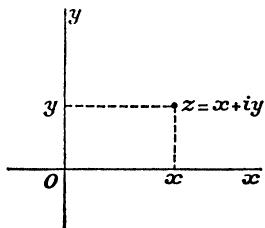
\includegraphics[keepaspectratio]{images/part001_cf49e1ad.jpg}}\\
图 7。

置换 \(z' \to \overline{z}\) （\(\mathbf{C}\) 的）是连续的，因此它是拓扑域 \(\mathbf{C}\) 的一个自同构。

事实上，它是拓扑域 C 中除恒等自同构外唯一的自同构（见习题 4）。

函数 \(\mathcal{R}(z)\) 、\(\mathfrak{J}(z)\) 正是 \(\mathbf{R}^2\) 到它的各因子上的投影，因此是连续的；绝对值 \(|z|\) 亦然，因为它是点 \((x,y)\) （在 \(\mathbf{R}^2\) 中）的欧氏范数（第六章，§ 2，第 1 号）。

绝对值的性质给出了 \(\mathbf{C}\) 的拓扑与其域结构相容这一事实的另一个证明（参看第九章，§ 3，第 2 号）；\(z + z'\) 的连续性由三角不等式 \(|z + z'| \leqslant |z| + |z'|\) 得出；\(zz'\) 的连续性由关系式

\[
\begin{array}{r l} | z z ^ {\prime} - z _ {0} z _ {0} ^ {\prime} | & = | z _ {0} (z ^ {\prime} - z _ {0} ^ {\prime}) + (z - z _ {0}) z _ {0} ^ {\prime} + (z - z _ {0}) (z ^ {\prime} - z _ {0} ^ {\prime}) | \\ & \leqslant | z _ {0} | \cdot | z ^ {\prime} - z _ {0} ^ {\prime} | + | z _ {0} ^ {\prime} | \cdot | z - z _ {0} | + | z - z _ {0} | \cdot | z ^ {\prime} - z _ {0} ^ {\prime} |; \end{array}
\]

得出；最后，\(z^{-1}\) 的连续性由关系式

\[
\left| z _ {0} ^ {- 1} - z ^ {- 1} \right| = | z | ^ {- 1}. \left| z - z _ {0} \right|. \left| z _ {0} \right| ^ {- 1}.
\]

\subsection{乘法群 C*}

我们从第三章 § 6 第 7 号知道，在非零复数的乘法群 \(\mathbf{C}^*\) 上诱导的拓扑与 \(\mathbf{C}^*\) 的群结构相容。由于 \(\mathbf{C}^*\) 在 \(\mathbf{C}\) 中是开的，由此得出 \(\mathbf{C}^*\) 是一个局部紧拓扑群（第一章，§ 9，第 7 号，命题 13），因而（关于乘法一致结构）是完备的；参看第三章，§ 6，第 8 号，命题 8）。乘法群 \(\mathbf{R}_+^*\) （\(>0\) 实数的）是 \(\mathbf{C}^*\) 的一个闭子群。另一个子群是绝对值为 1 的复数所成的集 \(\mathbf{U}\) ，它与单位圆周 \(\mathbf{S}_1\) （\(\mathbf{R}^2\) 的）等同，因此是一个紧群。此外：

命题 1. 拓扑群 \(\mathbf{C}^*\) 同构于拓扑群 \(\mathbf{R}^*\) 与 \(\mathbf{U}\) 的乘积。

因为映射 \(z \to \left( |z|, \frac{z}{|z|} \right)\) 是 \(\mathbf{C}^*\) 到 \(\mathbf{R}_+^* \times \mathbf{U}\) 上的一个同胚（第六章，§ 2，第 3 号，命题 3）；并且由此立即得出它是群结构的一个同构。

已经知道拓扑群 \(\mathbf{R}_{+}^{*}\) 同构于加法群 \(\mathbf{R}\) （第五章，§ 4，定理 1）；因此对拓扑群 \(\mathbf{C}^{*}\) 的研究就归结为对 \(\mathbf{U}\) 的研究，我们将在 § 2 中考虑它。

\subsection{四元数体}

由定理 1 推出，域 R 是一个极大有序域，因而（在同构意义下）R 上有限秩的唯一非交换除环就是 R 上的四元数体；它记作 H，称为实四元数体（或在无混淆之虞时简称四元数体）。由于 H 在域 R 上的秩为 4，我们可以在 H 上定义一个与 \(R^{4}\) 的拓扑同胚的拓扑（第六章，§ 1，第 5 号）。确切地说，我们通常把 H 与 \(R^{4}\) 等同，即把 H 的标准基的元素 1、i、j、k 分别等同于向量 \(e_{0}, e_{1}, e_{2}, e_{3}\) （\(R^{4}\) 的标准基的向量）。

我们回顾，H 的标准基的乘法表由下列公式给出

\[
\begin{array}{c} i ^ {2} = j ^ {2} = k ^ {2} = - \mathrm{I}, \quad i j = - j i = k, \\ j k = - k j = i, \quad k i = - i k = j. \end{array}
\]

H 的拓扑不仅与 H 的环结构相容（第六章，§ 1，第 5 号），而且与它的除环结构相容；因为若 x 是一个非零四元数，则 \(x^{-1}\) 的坐标是 x 的坐标的有理函数，其分母不为零。因此，赋有这一拓扑的除环 H 是一个非交换的拓扑除环。四元数 \(a + bi\) （a、b 为实数）构成 H 的一个（拓扑）子域，它同构于域 C，并常与 C 等同。

这样我们就有了局部紧、连通的拓扑除环的第三个例子，其余两个是 R 与 C。事实上，具有这两条性质的拓扑除环仅此三个。

我们从代数知道，四元数 \(x = x_{0} + x_{1}i + x_{2}j + x_{3}k\) 的约化范数是

\[
\mathrm{N} (\boldsymbol {x}) = x _ {0} ^ {2} + x _ {1} ^ {2} + x _ {2} ^ {2} + x _ {3} ^ {2} = | | \boldsymbol {x} | | ^ {2}
\]

（因此它是 x 的欧氏范数的平方）。由于

\[
\mathrm{N} (\boldsymbol {x y}) = \mathrm{N} (\boldsymbol {x}) \mathrm{N} (\boldsymbol {y}),
\]

由此得出，范数为 1 的所有四元数所成的集——它与球面 \(S_{3}\) 相同——构成非零四元数的乘法群 \(H^{*}\) 的一个紧子群。

命题 2. 非零四元数的乘法群 \(\mathbf{H}^*\) 是一个拓扑群，同构于它的子群 \(\mathbf{R}_+^*\) 与 \(\mathbf{S}_3\) 的乘积。

每个四元数 \(x \neq 0\) 都可以写成 \(x = ||x||.z\) ，其中 \(z\) 是范数为 1 的四元数；由于 \(||xx'|| = ||x||.||x'||\) ，映射 \(x \to (||x||, x/||x||)\) （\(H^*\) 到 \(R_+^* \times S_3\) 上的）是群结构的一个同构，并且由第六章 § 2 第 3 号命题 3，它是 \(H^*\) 到 \(R_+^* \times S_3\) 上的一个同胚。

注。1) 利用关系式 \(||x + y|| \leqslant ||x|| + ||y||\) 与 \(||xy|| = ||x||.||y||\) ，可以像第 2 号中对复数域那样直接证明 \(\mathbf{R}^4\) 的拓扑与 H 的除环结构相容（参看第九章，§ 3，第 2 号）。

\begin{enumerate}
\def\labelenumi{\arabic{enumi})}
\setcounter{enumi}{1}
\item
  由已证的结果推出，球面 \(S_{1}\) 与 \(S_{3}\) 能够带有与它们的拓扑相容的群结构。我们后面将看到，对每个异于 1 和 3 的整数 n，\(S_{n}\) 上不存在与 \(S_{n}\) 的拓扑相容的群结构。
\item
  群 \(\mathbf{S}_3\) 的每个点都有一个同胚于 \(\mathbf{R}^3\) 的邻域（第六章，§ 2，第 4 号，命题 5），但 \(\mathbf{S}_3\) 不局部同构于 \(\mathbf{R}^3\) ；因为若是这样，则由于它是连通的（第七章，§ 2，第 2 号，定理 1），它将是交换的，而事实并非如此，因为 \(i\) 与 \(j\) 都属于 \(\mathbf{S}_3\) 且 \(ij \neq ji\) （参看第五章，§ 3）。
\end{enumerate}

\section{角的测度，三角函数}

\subsection{乘法群 U}

定理 1. 绝对值为 1 的复数的（乘法）拓扑群 U 同构于模 1 实数的（加法）拓扑群 T。

\(\mathbf{U} = \mathbf{S}_{1}\) 是紧且连通的，并且它的单位元 \(+1\) 有一个同胚于 \(\mathbf{R}\) 的开区间的邻域（第六章，§ 2，第 4 号，命题 5）；因此该定理是第五章 § 3（定理 2）所给的 \(\mathbf{T}\) 的拓扑刻画的一个推论。

推论. 非零复数的乘法群 \(\mathbf{C}^*\) 同构于群 \(\mathbf{R} \times \mathbf{T}\) （参看 § 1. 第 3 号，命题 1）。

注. 群 \(C^{*}\) 与 \(R \times T\) 的同构蕴含着在域 C 中每个“二项方程” \(z^{n} = a\) 都有根。利用这一事实以及 C 的局部紧性，我们可以得到达朗贝尔–高斯定理的另一个证明（习题 2）。

从群 \(\mathbf{T}\) 到群 \(\mathbf{U}\) 上的不同同构只有两个；因为若 \(g\) 、\(g'\) 是 \(\mathbf{T}\) 到 \(\mathbf{U}\) 上的两个同构，而 \(h'\) 是 \(g'\) 的逆，则 \(h' \circ g\) 是 \(\mathbf{T}\) 的一个自同构，因而（第七章，§ 2，第 4 号，命题 6）我们恒有 \(g'(x) = g(x)\) 或 \(g'(x) = g(-x)\) 。我们总可以假设 \(g\) 使得 \(i\) 是 \(g\) 对模 \(1\) 类（点 \(\frac{1}{4}\) 的）所取的像；于是，若 \(\varphi\) 表示 \(\mathbf{R}\) 到 \(\mathbf{T}\) 上的典范同态，则加法群 \(\mathbf{R}\) 到乘法群 \(\mathbf{U}\) 上的每个严格态射都形如 \(x \to g(\varphi(x/a))\) ，其中 \(a\) 是一个 \(\neq o\) 的实数（第七章，§ 2，第 3 号，命题 4）；注意，区间 \([- \frac{1}{2} |a|, \frac{1}{2} |a|]\) 是 \(\mathbf{R}\) 中被这个严格态射一一地映到其像上的最大对称开区间，并且我们有 \(g(\varphi(\frac{1}{4})) = i\) 。我们将把同态 \(x \to g(\varphi(x))\) 记作 \(x \to e(x)\) ；因而 \(\mathbf{R}\) 到 \(\mathbf{U}\) 上的每个严格态射都形如 \(x \to e(x/a)\) ，其中 \(a \neq 0\) 。函数 \(e(x)\) 在 \(\mathbf{R}\) 上连续、取复值，并且满足恒等式

\begin{enumerate}
\def\labelenumi{(\arabic{enumi})}
\tightlist
\item
\end{enumerate}

\[
\left| e (x) \right| = 1,\tag{2}
\]

\[
\boldsymbol {e} (x + y) = \boldsymbol {e} (x) \boldsymbol {e} (y),
\]

以及关系式

\[
e (0) = \mathrm{I}, \quad e (\frac {1}{4}) = i, \quad e (\frac {1}{2}) = - \mathrm{I}, \quad e (\frac {3}{4}) = - i, \quad e (\mathrm{I}) = \mathrm{I}. \tag {3}
\]

由 (1) 与 (2) 得出

\[
e (- x) = \frac {1}{e (x)} = \overline {{{{e (x)}}}},\tag{4}
\]

而由 (2) 与 (3) 得出

\[
\begin{array}{l} e (x + \frac {1}{4}) = i e (x), \quad e (x + \frac {1}{2}) = - e (x), \\ e (x + \frac {3}{4}) = - i e (x), \quad e (x + 1) = e (x). \end{array}
\]

于是函数 \(e(x)\) 是周期的，并且以 1 为基本周期。

注. 映射 \(x + iy \to e^x e(y)\) 是加法群 \(\mathbf{C}\) 到乘法群 \(\mathbf{C}^*\) 上的一个严格态射，并且它在 \(\mathbf{o}\) 的一个适当邻域上的限制是 \(\mathbf{C}\) 与 \(\mathbf{C}^*\) 的一个局部同构。因而（第七章，§ 2，第 3 号）\(\mathbf{C}\) 到 \(\mathbf{C}^*\) 上的每个严格态射都形如 \(x + iy \to e^{\alpha x + \beta y} e(\gamma x + \delta y)\) ，其中 \(\alpha, \beta, \gamma, \delta\) 是使 \(\alpha \delta - \beta \gamma \neq \mathbf{o}\) 的任意实数。我们后面将看到，这些同态中恰有一个，记作 \(z \rightarrow e^{z}\) ，使得

\[
\lim _ {z \rightarrow 0} \frac {e ^ {z} - 1}{z} = 1;
\]

并且这个同态在实轴上的限制与 \(e^{x}\) 相同（由此得到该记号）。

\subsection{角}

由于域 \(\mathbf{R}\) 是有序的，我们可以定向实数平面 \(\mathbf{R}^2\) ，方法是取 \(e_1 \wedge e_2\) 为正二重向量（\(e_1, e_2\) 是标准基的向量）。于是，在定向的实数平面 \(\mathbf{R}^2\) （以下与 \(\mathbf{C}\) 等同）中，我们可以对任意一对射线定义角 \((\widehat{\Delta_1, \Delta_2})\) （射线对（ \(\Delta_1, \Delta_2\) ）以 \(o\) 为端点）(*)。所有角组成的集合 \(\mathfrak{A}\) 具有一个交换群结构（写成加法），由下式定义

\[
(\widehat {\Delta_ {1} , \Delta_ {3}}) = (\widehat {\Delta_ {1} , \Delta_ {2}}) + (\widehat {\Delta_ {2} , \Delta_ {3}}),
\]

于是特别有 \((\widehat{\Delta_1, \Delta_1}) = 0\) 且 \((\widehat{\Delta_2, \Delta_1}) = -(\widehat{\Delta_1, \Delta_2})\) 。

平角 \(\varpi\) 是 \(\neq 0\) 的解，即方程 \(2\theta = 0\) 在 \(\mathfrak{A}\) 中的解；它是负实半轴与正实半轴所成的角。

若 z 是任一非零复数，z 的辐角（或幅角），记作 \(\operatorname{Am}(z)\) ，是过 z 而以 o 为端点的射线与正实半轴所成的角。映射 \(z \to \operatorname{Am}(z)\) 是乘法群 \(C^{*}\) 到加法群 A 上的一个同态，因而我们有

\[
\operatorname{Am} \left(z z ^ {\prime}\right) = \operatorname{Am} (z) + \operatorname{Am} \left(z ^ {\prime}\right) \quad \text { and } \quad \operatorname{Am} (\bar {z}) = \operatorname{Am} \left(z ^ {- 1}\right) = - \operatorname{Am} (z).
\]

角 \(\delta = \operatorname{Am}(i)\) 称为正直角；它是方程 \(2\theta = \varpi\) 在 A 中的解之一，另一个解是 \(-\delta = \delta + \varpi\) 。

同态 \(z \to \operatorname{Am}(z)\) 限制到子群 \(\mathbf{U}\) （\(\mathbf{C}^*\) 的）上时，是 \(\mathbf{U}\) 的群结构到 \(\mathfrak{A}^{(**)}\) 的群结构上的一个同构；若用这个同构把 U 的拓扑转移到群 A 上，则后一群成为一个紧拓扑群，并且映射 \(z \to \operatorname{Am}(z)\) （\(C^{*}\) 到 A 上的）是拓扑群 \(C^{*}\) 到拓扑群 A 上的一个严格态射。

我们把 \(\theta \to f(\theta)\) 记为 \(\mathfrak{A}\) 到 \(\mathbf{U}\) 上的同构，它即同构 \(z \to \operatorname{Am}(z)\) （\(\mathbf{U}\) 到 \(\mathfrak{A}\) 上的）的逆。按定义，\(\mathcal{R}(f(\theta))\) 记作 \(\cos \theta\) ，称为角 \(\theta\) 的余弦；\(\mathfrak{J}(f(\theta))\) 记作 \(\sin \theta\) ，称为角 \(\theta\) 的正弦。这些函数在拓扑群 \(\mathfrak{A}\) 上连续，并且满足下列关系式（同处所引），它们是上述定义的直接推论：

\[
\begin{array}{r l} \cos o = 1, & \sin o = 0, \quad \cos \varpi = - 1, \quad \sin \varpi = 0, \\ \cos (- \theta) = \cos \theta , & \sin (- \theta) = - \sin \theta , \\ \cos (\theta + \theta^ {\prime}) = \cos \theta \cos \theta^ {\prime} - \sin \theta \sin \theta^ {\prime}, \\ \sin (\theta + \theta^ {\prime}) = \sin \theta \cos \theta^ {\prime} + \sin \theta^ {\prime} \cos \theta , \\ \cos^ {2} \theta + \sin^ {2} \theta = 1. \end{array}
\]

按定义，角 \(\theta \in \mathfrak{A}\) 的正切，当 \(\cos \theta \neq 0\) 时定义为 \(\sin \theta / \cos \theta\) （同处所引），记作 \(\tan \theta\) ；它是一个连续函数，由连续性延拓到 \(\tilde{\mathbf{R}}\) （第六章，§ 3，第 4 号），即取值 \(\infty\) 于角 \(\delta\) 与 \(-\delta\) 处。我们有 \(\tan (\theta + \varpi) = \tan \theta\) 。\(\theta\) 的余切，记作 \(\cot \theta\) ，是 \(\tilde{\mathbf{R}}\) 中等于 \(1 / \tan \theta\) 的元素。

注意，若 \(\operatorname{Am}(z) = \theta\) ，我们有 \(z = |z| (\cos \theta + i \sin \theta)\) ；这个表达式称为复数 \(z \neq 0\) 的三角形式。

\subsection{角的测度}

由第 1 号的定理 1，角的拓扑群 \(\mathfrak{A}\) 同构于 \(\mathbf{T}\) 。\(\mathbf{R}\) 到 \(\mathfrak{A}\) 上的每个严格态射都可由同构 \(z \to \operatorname{Am}(z)\) （\(\mathbf{U}\) 到 \(\mathfrak{A}\) 上的）与 \(\mathbf{R}\) 到 \(\mathbf{U}\) 上的一个严格态射复合而得；若令 \(\Im(x) = \operatorname{Am}(e(x))\) ，则 \(\mathbf{R}\) 到 \(\mathfrak{A}\) 上的每个严格态射都形如 \(x \to \Im(x/a)\) （ \(a \neq 0\) ）。给定一个一劳永逸地固定的实数 \(a > 0\) ，每个角 \(\theta\) 经同态 \(x \to \Im(x/a)\) 对应于实数模 \(a\) 的一个类（即 \(\mathbf{Z}/a\mathbf{Z}\) 的一个元素），它称为 \(\theta\) 相对于底 \(a\) 的测度；按惯用说法，该类中的每个实数也称为 \(\theta\) 的一个测度；角 \(\Im(x/a)\) 称为（相对于底 a）测度为 \(x\) 的角。若 x 是 \(\theta\) 的一个测度而 \(x'\) 是 \(\theta'\) 的一个测度（相对于同一个底），则 \(x + x'\) 是 \(\theta + \theta'\) 的一个测度，且 -x 是 - \(\theta\) 的一个测度。角（相对于底 a）的主测度是其位于区间 {[}0, a{]} 中的那个测度。

底 \(a\) 的选取。我们总限于取 \(a > 1\) 的底。每个 \(a > 1\) 对应一个角 \(\omega = \Im(1/a)\) ，它的主测度是 \(1\) ，称为相对于底 \(a\) 的角的测度单位；反之，每个角 \(\omega \neq 0\) 对应唯一的 \(a > 1\) 使 \(\Im(1/a) = \omega\) ，因此知道角的测度单位就完全确定了底 \(a > 1\) 。

在数值计算中通常取 \(a = 360\) 或 \(a = 400\) ；相应的角的测度单位称为度（ \(a = 360\) ）或百分度（ \(a = 400\) ）。

在分析中，以及在一切不涉及数值计算的数学分支中，普遍使用由条件

\[
\lim _ {x \rightarrow 0} \frac {e (x / a) - 1}{x} = 1
\]

所定义的底 a；这个底记作 \(2\pi\) 。相应的角的测度单位称为弧度，其测度称为弧度测度；利用前面提到的对复数 z 的 \(e^{z}\) 的定义，我们有 \(\boldsymbol{e}(x)=e^{2\pi ix}\) 对一切 \(x\in R\) 成立。

底 a 一经选定，当人们说到一个角时，通常指的就是这个角相对于底 a 的一个测度；只要（在不涉及数值计算时情形总是如此）底 a 自始至终保持固定，并且记住模 a 同余的两个实数对应于同一个角，这种惯用说法并无妨碍。

例如，通常所理解的复数 \(z \neq 0\) 的辐角，是指该角的一个弧度测度，它由依所考虑的问题而定的约定来确定；这些约定一经作出，如此选定的辐角的测度就记作 Am (z)。

\subsection{三角函数}

若把（定义在 A 上的）函数 \(\cos\theta\) 、\(\sin\theta\) 、\(\tan\theta\) 、\(\cot\theta\) 与 R 到 A 上的同态 \(x\to\Im(x/a)\) 复合，则如此得到的函数

\[
\cos \Im \left(\frac {x}{a}\right), \quad \sin \Im \left(\frac {x}{a}\right), \quad \tan \Im \left(\frac {x}{a}\right), \quad \cot \Im \left(\frac {x}{a}\right)
\]

分别称为数 \(x\) 相对于底 \(a\) 的余弦、正弦、正切与余切，并记作 \(\cos_a x\) 、\(\sin_a x\) 、\(\tan_a x\) 、\(\cot_a x\) 。映射 \(x \to \cos_a x + i \sin_a x\) 是 \(\theta \to \cos \theta + i \sin \theta\) 与 \(x \to \Im(x/a)\) 的复合，因而由第 2 号中 \(\cos \theta\) 与 \(\sin \theta\) 的定义，我们有恒等式

\[
e \left(\frac {x}{a}\right) = \cos_ {a} x + i \sin_ {a} x,\tag{5}
\]

它等价于

\[
\cos_ {a} x = \Re \left(e \left(\frac {x}{a}\right)\right), \quad \sin_ {a} x = \Im \left(e \left(\frac {x}{a}\right)\right),
\]

并且由 (4)，它也等价于

\[
\cos_ {a} x = \frac {\mathrm{I}}{2} \left(e \left(\frac {x}{a}\right) + e \left(- \frac {x}{a}\right)\right), \quad \sin_ {a} x = \frac {\mathrm{I}}{2 i} \left(e \left(\frac {x}{a}\right) - e \left(- \frac {x}{a}\right)\right).
\]

由此得到恒等式

\[
\cos_ {b} x = \cos_ {a} \left(\frac {a x}{b}\right), \quad \sin_ {b} x = \sin_ {a} \left(\frac {a x}{b}\right).\tag{6}
\]

在不涉及数值计算的数学分支中所出现的三角函数，只有上述相对于基 \(2\pi\) 的那些函数；这些函数简单地记作 \(\cos x\) 、\(\sin x\) 、\(\tan x\) 、\(\cot x\) ，以代替 \(\cos_{2\pi}x\) 、\(\sin_{2\pi}x\) 、\(\tan_{2\pi}x\) 、\(\cot_{2\pi}x\) 。出于数值计算的目的，有对应于基 a = 360 与 a = 400 的三角函数表；而公式 (6) 使我们能推出相对于任何其他基的三角函数的值。

前面回忆过的角的余弦与正弦之间的关系，显然给出度量这些角的数之间的同样的关系；特别地，我们有

\[
\begin{array}{r l} & {\cos_ {a} (x + y) = \cos_ {a} x \cos_ {a} y - \sin_ {a} x \sin_ {a} y,} \\ & {\sin_ {a} (x + y) = \sin_ {a} x \cos_ {a} y + \sin_ {a} y \cos_ {a} x,} \\ & {\cos_ {a} (- x) = \cos_ {a} x, \qquad \sin_ {a} (- x) = - \sin_ {a} x,} \\ & {\qquad \cos_ {a} ^ {2} x + \sin_ {a} ^ {2} x = 1.} \end{array}
\]

函数 \(\cos_{a}x\) 与 \(\sin_{a}x\) 在 R 上连续，并且以 a 为周期；此外，a 是这些函数的基本周期，因为关系 \(\cos_{a}x = \cos_{a}y\) 蕴含或者 \(\sin_{a}x = \sin_{a}y\) ，或者

\[
\sin_ {a} x = - \sin_ {a} y, \quad \text { i.e., }
\]

\[
e \left(\frac {x}{a}\right) = e \left(\frac {y}{a}\right) \quad \text { or } \quad e \left(\frac {x}{a}\right) = e \left(- \frac {y}{a}\right),
\]

从而或者

\[
x \equiv y (\mathrm{mod} a) \quad \text { or } \quad x \equiv - y (\mathrm{mod} a);
\]

而类似地，

\[
\sin_ {a} x = \sin_ {a} y
\]

等价于 \(x \equiv y \pmod{a}\) 或者 \(x + y \equiv \frac{1}{2} a \pmod{a}\) 。

由此可知，\(\cos_{a}x\) 在区间 \([0,\frac{1}{2}a]\) 中绝不两次取同一个值；因此，当限制在这个区间上时，它是该区间到区间 \([-1,+1]\) 上的一个双射映射。由于 \(\cos_{a}0=1\) 且 \(\cos_{a}\left(\frac{1}{2}a\right)=-1\) ，故 \(x\to\cos_{a}x\) 是 \([0,\frac{1}{2}a]\) 到 \([-1,1]\) 上的一个严格递减映射（第四章，§ 2，第 6 号，定理 5 及其注）。\(\cos_{a}x=0\) （当 x=a/4），\(\cos_{a}x>0\) 对 \(0\leqslant x<a/4\) 成立，\(\cos_{a}x<0\) 对 \(a/4<x\leqslant a/2\) 成立。由 \(\cos_{a}(-x)=\cos_{a}x\) 可以推出 \(\cos_{a}x\) 在区间 \([-\frac{1}{2}a,0]\) 中的变化情况，从而由周期性推出它在整个 R 上的变化情况（图 8）。由 \(\sin_{a}x=-\cos_{a}(x+a/4)\) 又可推出 \(\sin_{a}x\) 在 R 中的变化情况（图 8）。

\pandocbounded{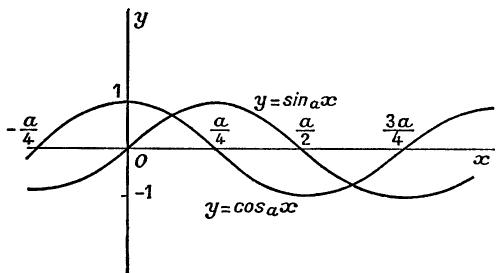
\includegraphics[keepaspectratio]{images/part001_7529c0a8.jpg}}\\
图 8.

函数 \(\tan_{a}x\) 是 \(\mathbf{R}\) 到 \(\tilde{\mathbf{R}}\) 上的一个连续映射；它取值 \(\infty\) 于诸值 \(\frac{1}{4} a + \frac{1}{2} ka\) 处（ \(k \in \mathbf{Z}\) ）。由于 \(\frac{1}{2} a\) 是 \(\tan_{a}x\) 的一个周期，故它是一个基本周期。在区间 \([0, \frac{1}{4} a]\) 中，\(\sin_{a}x\) 从 \(0\) 递增到 \(1\) ，\(\cos_{a}x\) 从 \(1\) 递减到 \(0\) ，因此 \(\tan_{a}x\) 在 \([0, \frac{1}{4} a[\) 中严格递增，并把这个区间映射到 \([0, +\infty[\) 上；由此推出 \(\tan_{a}x\) 在区间 \(]-\frac{1}{4}a,+\frac{1}{4}a[.\) 中严格递增，并且是这个区间到 R 上的一个同胚（图 9）。

\pandocbounded{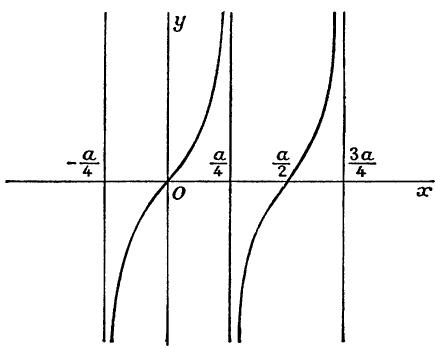
\includegraphics[keepaspectratio]{images/part001_329f289a.jpg}}\\
图 9.

\subsection{角域}

给定两条不同的闭射线 \(\Delta_{1}, \Delta_{2}\) ，其端点为 \(o\) ，设 \(x\) 为角 \((\widehat{\Delta_{1}, \Delta_{2}})\) 的主测度（相对于一个基 \(a\) ，一经选定便不再改变）。闭（相应地开）射线 \(\Delta\) （以 \(o\) 为端点）当中，其主测度 \(y\) （角 \((\widehat{\Delta_{1}, \Delta})\) 的）满足 \(o \leqslant y \leqslant x\) （相应地 \(o < y < x\) ）者的并集，就是代数中所定义的闭（相应地开）角域 \(S\) （以 \(\Delta_{1}\) 为始边、以 \(\Delta_{2}\) 为终边）。因为借助于一个旋转，总可以化归为 \(S\) 不包含过点 \(-1\) 的射线的情形。若 \(\alpha\) 与 \(\beta\) 此时是 \(\Delta_{1}\) 与 \(\Delta_{2}\) 分别与实正半轴所成的角，则闭角域 \(S\) 是诸闭半直线 \(\Delta\) 的并，这些半直线与实正半轴成角 \(\theta\) ，使得 \(\tan \frac{1}{2} \alpha \leqslant \tan \frac{1}{2} \theta \leqslant \tan \frac{1}{2} \beta\) 。而若 \(u, v, t\) 分别是 \(\alpha, \beta, \theta\) 的属于区间 \([- \frac{1}{2} a, + \frac{1}{2} a[\) 的测度，则这些不等式等价于 \(\tan_{a} \frac{1}{2} u \leqslant \tan_{a} \frac{1}{2} t \leqslant \tan_{a} \frac{1}{2} v\) ；又由于 \(\tan_{a} x\) 在区间 \([- \frac{1}{4} a, + \frac{1}{4} a[\) 中是递增函数，它们也等价于 \(u \leqslant t \leqslant v\) ，或等价于 \(o \leqslant t - u \leqslant v - u\) ；由于 \(x = v - u\) ，\(y = t - u\) ，于是结论对闭角域得证，而对开角域的证明是类似的。

闭角域是 \(R^{2}\) 中的闭集，而与它有同一始边和同一终边的开角域是它在 \(R^{2}\) 中的内部（第六章，§ 2，第 3 号，命题 3）。角 \((\widehat{\Delta_1, \Delta_2})\) （其主测度为 \(x\) ）称为角域 S 的角；当 \(x < \frac{1}{2} a\) 时称 S 为凸角域，当 \(x = \frac{1}{2} a\) 时称为平角域（即闭半平面），当 \(x > \frac{1}{2} a\) 时称为凹角域。凸角域当 \(x < \frac{1}{4} a\) 时为锐角域，当 \(x = \frac{1}{4} a\) 时为直角域，当 \(x > \frac{1}{4} a\) 时为钝角域。角域 S 的平分线是射线 \(\Delta\) ，它以 \(y = \frac{1}{2} x\) 为其与 \(\Delta_1\) 所成的角。

\pandocbounded{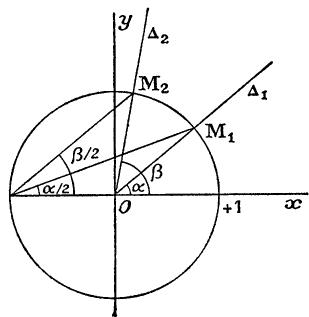
\includegraphics[keepaspectratio]{images/part001_1c4c55ab.jpg}}\\
图 10.

两条不同的闭射线 \(\Delta_{1}, \Delta_{2}\) 确定两个闭角域；它们的并是实平面 \(R^{2}\) ，而它们的交是 \(\Delta_{1} \cup \Delta_{2}\) 。

\subsection{叉角}

我们也在代数中定义过极大有序域上的二维向量空间中一对直线的叉角（*）。这个定义特别适用于实平面 \(\mathbf{R}^2\) 。全体叉角的集合 \(\mathfrak{A}_0\) 具有一个交换群结构（写成加法），它由下式定义

\[
(\widehat {\mathbf {D _ {1} , D _ {3}}}) = (\widehat {\mathbf {D _ {1} , D _ {2}}}) + (\widehat {\mathbf {D _ {2} , D _ {3}}})
\]

因而特别有 \((\widehat{\mathbf{D}_1,\mathbf{D}_1}) = 0\) 与 \((\widehat{\mathbf{D}_2,\mathbf{D}_1}) = -(\widehat{\mathbf{D}_1,\mathbf{D}_2}).\)

直叉角 \(\delta_0\) 是 \(\neq 0\) 的、方程 \(2\theta = 0\) 在 \(\mathfrak{A}_0\) 中的解；它是虚轴与实轴所成的叉角。

我们定义一个典范同态 \(\varphi\) ：由角群 \(\mathfrak{A}\) 到叉角群 \(\mathfrak{A}_0\) 上，它把射线 \(\Delta\) 与实正半轴所成的角，对应为包含 \(\Delta\) 的直线 D 与实轴所成的叉角。一个叉角 \(\theta_0\) 是 \(\varphi\) 下两个角 \(\theta\) 与 \(\theta + \varpi\) 的像；于是 \(\mathfrak{A}_0\) 同构于 \(\mathfrak{A}\) 对子群 \(\{o, \varpi\}\) 的商群。若在 \(\mathfrak{A}_0\) 上转移商群 \(\mathfrak{A}/\{o, \varpi\}\) 的拓扑（借助与 \(\varphi\) 相伴的双射同态来转移），则 \(\mathfrak{A}_0\) 成为一个紧拓扑群，而 \(\varphi\) 成为 \(\mathfrak{A}\) 到 \(\mathfrak{A}_0\) 上的一个严格态射。

如果把同态 \(\varphi\) （ \(\mathfrak{A}\) 到 \(\mathfrak{A}_0\) 上的）与同态 \(x \to \Im(x/a)\) （ \(\mathbf{R}\) 到 \(\mathfrak{A}\) 上的）复合，就得到一个同态 \(x \to \Im_0(x/a)\) （ \(\mathbf{R}\) 到 \(\mathfrak{A}_0\) 上的）；每个叉角 \(\theta_0 \in \mathfrak{A}_0\) 在这个同态之下对应于实数的一个模 \(\frac{1}{2}a\) 的类，它称为叉角 \(\theta_0\) 的测度（相对于基 \(a\) ）；照惯用说法，这个类中的每个数都称为 \(\theta_0\) 的一个测度，而其中属于区间 \([0, \frac{1}{2}a]\) 的那个称为 \(\theta_0\) 的主测度；叉角 \(\Im_0(x/a)\) 是测度为 \(x\) 的叉角。\(\theta_0\) 的每个测度也是角 \(\theta, \theta + \varpi\) 二者之一的一个测度，这两个角在同态 \(\varphi\) 下的像是 \(\theta_0\) 。

这里同样地，一旦选定了基 a ，当我们谈到一个叉角时，照惯用说法，一般指相对于基 a 的这个叉角的一个测度。

注。我们可以定义 \(\mathbf{C}^*\) 到 \(\mathfrak{A}_0\) 上的一个同态，它把每个复数 \(z \neq 0\) 映为过 \(0\) 与 \(z\) 的直线与实轴所成的叉角。显然这个同态是 \(\varphi\) 与同态 \(z \to \operatorname{Am}(z)\) （ \(\mathbf{C}^*\) 到 \(\mathfrak{A}\) 上的）的复合；因此它是拓扑群 \(\mathbf{C}^*\) 到拓扑群 \(\mathfrak{A}_0\) 上的一个严格态射，而与之相伴的双射同态是商群 \(\mathbf{C}^*/\mathbf{R}^*\) 到 \(\mathfrak{A}_0\) 上的一个同构。

我们知道，若 D 表示一条与实轴成叉角 \(\theta_0\) 的直线，且 \((a, b)\) 是 D 的一对方向比，则叉角 \(\theta_0\) 的正切（记作 tan \(\theta_0\) ）是元素 \(b/a\) （ \(\tilde{\mathbf{R}} (= \infty\) 若 \(a = 0\) ），它也称为直线 D 的斜率。若 \(\theta\) 与 \(\theta + \varpi\) 是在 \(\varphi\) 下以 \(\theta_0\) 为像的两个角，则有 \(\tan \theta_0 = \tan \theta = \tan (\theta + \varpi)\) 。映射 \(\theta_0 \to \tan \theta_0\) 是 \(\mathfrak{A}_0\) 到 \(\tilde{\mathbf{R}}\) 上的一个同胚，因为拓扑空间 \(\mathbf{C}^*/\mathbf{R}^*\) 正是实射影直线 \(\mathbf{P}_1\) ，而且由第六章 § 3 第 3 号，把直线（视为 \(\mathbf{P}_1\) 的点）对应到其斜率的映射是 \(\mathbf{P}_1\) 到 \(\tilde{\mathbf{R}}\) 上的一个同胚。现在，若在 \(\tilde{\mathbf{R}}\) 上转移 \(\mathfrak{A}_0\) 的群结构（借助映射 \(\theta_0 \to \tan \theta_0\) 来转移），我们就在 \(\tilde{\mathbf{R}}\) 上定义了一个交换拓扑群的结构，其中两个元素 \(t_1\) 、\(t_2\) 的积是 \(\frac{t_1 + t_2}{1 - t_1 t_2}\) ，只要 \(t_1\) 、\(t_2\) 属于 R 且 \(t_1 t_2 \neq 1\) ；对不满足这些条件的数对 \((t_1, t_2)\) ，\(t_{1}\) 与 \(t_{2}\) 的积通过把函数 \(\frac{x+y}{1-xy}\) 连续地延拓到 \(\tilde{R}\times\tilde{R}\) 而得到，并且仍记作 \(\frac{t_{1}+t_{2}}{1-t_{1}t_{2}}\) 。

\section{复数的无穷和与无穷乘积}

\subsection{复数的无穷和}

由于域 C 的加法群与加法群 \(R^{2}\) 相同，无须对 C 中的可和族与级数作专门研究，因为这已包含在第七章 § 3 的一般理论之中；我们把这理论的结果翻译成复数理论的语言这一练习留给读者。我们只叙述下面的命题，它是第七章 § 3 第 1 号命题 3 的一个推论：

命题 1 。若 \((u_{\lambda})_{\lambda \in \mathbf{L}}\) 与 \((v_{\mu})_{\mu \in \mathbf{M}}\) 是两个复数的可和族，则族 \((u_{\lambda}v_{\mu})_{(\lambda ,\mu)\in \mathbf{L}\times \mathbf{M}}\) 可和，且有

\[
\sum_ {(\lambda , \mu) \in \mathbf {L} \times \mathbf {M}} u _ {\lambda} v _ {\mu} = \left(\sum_ {\lambda \in \mathbf {L}} u _ {\lambda}\right) \left(\sum_ {\mu \in \mathbf {M}} v _ {\mu}\right).\tag{1}
\]

把关于四元数的相应结果的叙述留给读者。

\subsection{\texorpdfstring{\(C^*\) 中的可乘族}{复数乘法群中的可乘族}}

在非零复数的乘法群 \(\mathbf{C}^*\) 中，一个族 \((z_{i})_{i\in I}\) 只有当 \(\lim z_{i} = 1\) （关于 \(I\) 的有限子集的余集所成的滤子）时才可能是可乘的（第三章，§ 5，第 2 号，命题 1）；此外，由于 \(\mathbf{C}^*\) 的每一点都有可数的基本邻域系，指标 \(i\) （满足 \(z_{i}\neq 1\) 者）所成的集合当族 \((z_{i})\) 可乘时是可数的（第三章，§ 5，第 2 号，命题 1 的推论）。

命题 2 。复数的一个族 \((z_{t})\) ，其中 \(z_{t} = r_{t}(\cos \theta_{t} + i\sin \theta_{t})\) ，它是可乘的，当且仅当族 \((r_{t})\) （诸 \(z_{t}\) 的绝对值所成的）在 \(\mathbf{R}_{+}^{*}\) 中可乘，且族 \((\theta_{t})\) （诸 \(z_{t}\) 的辐角所成的）在角群 \(\mathfrak{A}\) 中可和。

鉴于群 \(\mathbf{C}^*\) 的结构（ \(\S\) 1，第 3 号，命题 1），本命题是第三章 \(\S\) 5 第 4 号命题 4 的直接推论。

若把每个角 \(\theta\) 映到它的（对任给基 \(a\) 而言的）属于区间 \([- \frac{1}{2} a, \frac{1}{2} a]\) 的那个测度，就得到 \(\mathfrak{A}\) 与 \(\mathbf{R}\) 的一个局部同构（ \(\S 2\) ，第 2 号）；由于 \(\lim \theta_{t} = 0\) （关于 \(\mathbf{I}\) 的有限子集的余集所成的滤子），我们可以把（命题 2 陈述中的）族 \(\theta_t\) 在 \(\mathfrak{A}\) 中可和这一条件，换成这样的条件：族 \((t_t)\) （诸角 \(\theta_t\) 的、属于 \([- \frac{1}{2} a, \frac{1}{2} a]\) 的测度所成之族）在 \(\mathbf{R}\) 中可和。

下述定理给出了形如 \((\mathbf{1} + u_{\iota})\) 的复数族在 \(\mathbf{C}^*\) 中可乘的另一个判别法。（它推广了第四章 § 7 第 4 号的定理 4；并参见第九章附录第 2 号命题 1：）

定理 1 。族 \((\mathbf{1} + u_{\iota})_{\iota \in \mathbf{I}}\) 在 \(\mathbf{C}^*\) 中可乘的充分必要条件是：族 \((|u_{\iota}|)\) 在 \(\mathbf{R}\) 中可和。

对 I 的每个有限子集 J，令

\[
p _ {J} = \prod_ {\iota \in J} (\mathbf{1} + a _ {\iota}), \quad s _ {J} = \sum_ {\iota \in J} a _ {\iota}, \quad \sigma_ {J} = \sum_ {\iota \in J} | a _ {\iota} |.
\]

引理 1 。对 I 的每个有限子集 J，令 \(\varphi(J) = \sup_{L \subset J} (p_L - 1)\) 。则对 J 的每个子集 L，我们有

\[
\left| p _ {\mathbf {L}} - \mathbf {1} - s _ {\mathbf {L}} \right| \leqslant \varphi (\mathrm{J}) \sigma_ {\mathbf {L}}.\tag{2}
\]

当 L 为空集时这是明显的。我们对 card (L) 作归纳。设 \(L = K \cup \{\lambda\}\) ，其中 \(\lambda \notin K\) ；则 \(p_{\mathbf{L}} = p_{\mathbf{K}}(\mathbf{1} + a_{\lambda})\) 且 \(s_{\mathbf{L}} = s_{\mathbf{K}} + a_{\lambda}\)，从而 \(p_{\mathbf{L}} - \mathbf{1} - s_{\mathbf{L}} = (p_{\mathbf{K}} - \mathbf{1} - s_{\mathbf{K}}) + (p_{\mathbf{K}} - \mathbf{1})a_{\lambda}\) ；于是由归纳假设与 \(\varphi(\mathbf{J})\) 的定义，有

\[
\left| p _ {\mathrm{L}} - \mathrm{1} - s _ {\mathrm{L}} \right| \leqslant \varphi (\mathrm{J}) \sigma_ {\mathrm{K}} + \varphi (\mathrm{J}) \left| a _ {\lambda} \right| = \varphi (\mathrm{J}) \sigma_ {\mathrm{L}},
\]

这就证明了引理。

引理 2 。若 J 是 I 的使 \(\varphi(J) < 1/4\) 的有限子集，则

\[
\left| \sigma_ {J} \right| \leqslant 4 \varphi (J) / (1 - 4 \varphi (J)).
\]

因为 \(\sigma_{\mathbf{L}} \leqslant \sigma_{\mathbf{J}}\) 对子集 \(\mathbf{L}\) （ \(\mathbf{J}\) 的每一个）成立，故由 (2) 得 \(|s_{\mathbf{L}}| \leqslant \varphi(\mathbf{J})\sigma_{\mathbf{J}} + |p_{\mathbf{L}} - \mathbf{1}| \leqslant (\mathbf{1} + \sigma_{\mathbf{J}})\varphi(\mathbf{J})\) ；但由第七章 §3 第 1 号命题 2，有 \(|\sigma_{\mathbf{J}}| \leqslant 4\sup_{\mathbf{L} \subset \mathbf{J}} |s_{\mathbf{L}}|\) ，从而 \(\sigma_{\mathbf{J}} \leqslant 4\varphi(\mathbf{J})(\mathbf{1} + \sigma_{\mathbf{J}})\) ，由此即得结论。

现在来证明定理 1 所述的条件是充分的。族 \((|u_{\iota}|)\) 在 \(\mathbf{R}\) 中可和这一假设蕴含族 \((\mathrm{1} + |u_{\iota}|)\) 在 \(\mathbf{R}_{+}^{*}\) 中可乘（第四章，§ 7，第 4 号，定理 4）；因此，对每个 \(\varepsilon > 0\) ，存在 I 的有限子集 \(J_{0}\) ，使得对每个不与 \(J_{0}\) 相交的 I 的有限子集 L，有 \(\prod_{\iota \in L} (\mathrm{1} + |u_{\iota}|) - \mathrm{1} \leqslant \varepsilon\) 。但我们可以把 \(\prod_{\iota \in L} (\mathrm{1} + u_{\iota}) - \mathrm{1}\) 写成 \(\sum_{M} \left( \prod_{\iota \in M} u_{\iota} \right)\) 的形式，其中 M 取遍 L 的所有非空子集；而由于 \(\left| \prod_{\iota \in M} u_{\iota} \right| = \prod_{\iota \in M} |u_{\iota}|\) ，我们有

\[
\left| \prod_ {\iota \in L} (1 + u _ {\iota}) - 1 \right| \leqslant \sum_ {M} \left(\prod_ {\iota \in M} | u _ {\iota} |\right) = \prod_ {\iota \in L} (1 + | u _ {\iota} |) - 1 \leqslant \varepsilon .
\]

由于 \(\mathbf{C}^*\) 是完备群，根据柯西判别法，这就证明了我们的断言。

还须证明定理 1 的条件是必要的。若 \((\mathbf{1} + u_{\iota})_{\iota\in \mathbf{I}}\) 是 \(\mathbf{C}^*\) 中的可乘族，则存在一个有限子集 \(J\) （ \(I\) 的），使得对每个有限子集 \(H\) （ \(I\) 的、不与 \(J\) 相交的），有 \(\left|\prod_{\iota\in H}(1 + u_{\iota}) - 1\right| \leqslant 1/8\) 。由引理 2 推出，\(\sum_{\iota\in H}|u_{\iota}| \leqslant 1\) 对每个有限子集 \(H\) （ \(I\) 的、不与 \(J\) 相交的）成立，因而族 \((|u_{\iota}|)\) 在 \(\mathbf{R}\) 中可和（第四章，§ 7，第 1 号，定理 1）。

上面的证明经过适当修改，也适用于某些非交换除环和代数中的（有序）无穷乘积（见习题 6 及第九章附录）。

\subsection{复数的无穷乘积}

为使以 \(z_{n} = r_{n}(\cos \theta_{n} + i\sin \theta_{n})\) 为通项的非零复数的无穷乘积在 \(\mathbf{C}^{*}\) 中收敛，根据群 \(\mathbf{C}^{*}\) 的结构，必要且充分的是：以 \(r_{n}\) 为通项的乘积在 \(\mathbf{R}_{+}^{*}\) 中收敛，且以 \(t_{n}\) 为通项的级数（即 \(\theta_{n}\) 的属于 \(] - \frac{1}{2} a, \frac{1}{2} a]\) 的测度）在 \(\mathbf{R}\) 中收敛。

定义 1 。以 \(1 + u_{n}\) 为通项的复数无穷乘积称为绝对收敛的，如果以 \(1 + |u_{n}|\) 为通项的乘积收敛（或者等价地，以 \(|u_{n}|\) 为通项的级数收敛）。

命题 3 。复数的无穷乘积交换收敛，当且仅当它绝对收敛。

这由第三章 § 5 第 7 号的命题 9 及上面第 2 号的定理 1 得出。

注。1) 以 \(|1 + u_n|\) 为通项的乘积可以在 \(\mathbf{R}_+^*\) 中收敛甚至绝对收敛，而以 \(1 + |u_n|\) 为通项的乘积不收敛（见习题 4）；当然，若诸 \(u_n\) 从某个下标起都是实数且 \(>0\) ，这种情形不会发生。

\begin{enumerate}
\def\labelenumi{\arabic{enumi})}
\setcounter{enumi}{1}
\tightlist
\item
  正如对因子 \textgreater0 的乘积已指出的，以 \(u_{n}\) 为通项的级数的收敛性，对于以 \(1 + u_{n}\) 为通项的乘积的收敛性既不必要也不充分。
\end{enumerate}

\section{复数空间与射影空间}

\subsection{\texorpdfstring{向量空间 \(C^{n}\)}{向量空间 C 的 n 次幂}}

由于拓扑空间 \(\mathbf{C}\) 可与 \(\mathbf{R}^2\) 等同，拓扑积 \(\mathbf{C}^n\) （ \(n\) 个与 \(\mathbf{C}\) 全同的空间之积）作为拓扑空间可与 \(\mathbf{R}^{2n}\) 等同；同样，\(\mathbf{C}^n\) 的拓扑群结构（即 \(n\) 个因子的加法（拓扑）群结构之积）可与加法群 \(\mathbf{R}^{2n}\) 的结构等同。但由于 \(\mathbf{C}\) 是一个域，我们可以在 \(\mathbf{C}^n\) 上定义 \(n\) 维向量空间（在 \(\mathbf{C}\) 上）的结构：积 \(az\) （复数 \(a\) 与点 \(z = (z_i)\) （属于 \(\mathbf{C}^n\) ）的积）是点 \((az_i)\) ；这个向量空间结构应仔细地与 \(2n\) 维向量空间（ \(\mathbf{R}\) 上的、定义在 \(\mathbf{R}^{2n}\) 上的）结构区别开来（第六章，§ 1，第 3 号）。我们将把记号 \(\mathbf{C}^n\) 保留给 \(n\) 个与 \(\mathbf{C}\) 全同的空间之积所成的拓扑空间，它还带有刚才定义的 \(\mathbf{C}\) 上的向量空间结构；\(\mathbf{C}^n\) 称为 \(n\) 维复数空间。注意，映射 \((t, z) \to tz\) 在 \(\mathbf{C} \times \mathbf{C}^n\) 上是连续的。

\(C^{n}\) 到 \(C^{m}\) 中的仿射线性映射也是 \(R^{2n}\) 到 \(R^{2m}\) 中的仿射线性映射，但反之不真。

例如，映射 \(z \rightarrow \overline{z}\) 是向量空间 \(R^{2}\) 到其自身上的线性映射，但不是向量空间 C 到其自身上的线性映射。

因此，\(C^{n}\) 到 \(C^{m}\) 中的每个仿射线性映射都一致连续；特别地，\(C^{n}\) 到其自身上的每个仿射线性映射都是同胚。

每个 p 维 \((p \leqslant n)\) 的仿射线性簇（在向量空间 \(C^{n}\) 中）也是向量空间 \(R^{2n}\) 中的一个 2p 维仿射线性簇；这里同样，反之不真。为避免一切混淆，\(C^{n}\) 中的 p 维（仿射）线性簇将称为 p 维复线性簇（\(R^{2n}\) 中的线性簇在为避免误解而需要时称为实线性簇）。特别地，一维（相应地二维）复线性簇称为复直线（相应地复平面），而 n - r 维复线性簇称为复超平面。

把实数空间 \(R^{n}\) 看作嵌入在复数空间 \(C^{n}\) 之中，这常常是方便的，其作法是把 \(R^{n}\) 与 \(C^{n}\) 的一个子集（由关系式 \(\mathfrak{J}(z_{k}) = o\) （ \(1 \leqslant k \leqslant n\) ）所定义的）等同起来。\(C^{n}\) 的拓扑群结构在这个子集上诱导的拓扑群结构与 \(R^{n}\) 的拓扑群结构一致。

注意，\(R^{n}\) （这样嵌入在 \(C^{n}\) 中的）不是 \(C^{n}\) 中的复线性簇。

\(R^{n}\) 中 p 个向量组成的一个系，若在 R 上是自由的，则在 C 上也是自由的。\(R^{n}\) 中每个 p 维实线性簇 V 生成一个 p 维复线性簇 \(V'\) （在 \(C^{n}\) 中），使得 V 是 \(V'\) 在 \(R^{n}\) 上的迹；若 V 由 n-p 个线性方程 \(f_{k}(x)=a_{k}\) 组成的一个方程组所定义，其中诸 \(f_{k}\) 是 \(R^{n}\) 上的线性型（具有实系数且在 R 上线性无关），而诸 \(a_{k}\) 是实数，则同样的方程组定义 \(V'\) ，只是现在 x 的坐标取复数值。

反之，若一个 \(p\) 维复线性簇与 \(\mathbf{R}^n\) 有非空的交，则这个交是一个实线性簇，但其维数可以 \(< p\) 。

\subsection{域 C 上向量空间与代数的拓扑}

第六章 § 1 第 5、6 号中关于域 R 上向量空间与代数的拓扑（特别是元素在 R 中的矩阵的空间与代数）的所有定义和所有结果，当我们处处把 R 换成 C 时，都毫无修改地保持有效。

\subsection{复射影空间}

采用第六章 § 3 第 1 号中回忆过的记号，我们给出与实射影空间的定义类似的下述定义：

定义 1 。射影空间 \(\mathbf{P}_{n}(\mathbf{C})\) ，带有可能作为 \(\mathbf{C}_{n+1}^{*}\) 的拓扑对等价关系 \(\Delta_{n}(\mathbf{C})\) 的商的那个拓扑，称为 \(n\) 维复射影空间。

射影空间 \(\mathbf{P}_{1}(\mathbf{C})\) 称为复射影直线，\(\mathbf{P}_{2}(\mathbf{C})\) 称为复射影平面。

关于实射影空间的大部分论证，只需作很小的修改即可推广到复射影空间。

首先我们看到，拓扑空间 \(\mathbf{P}_{n}(\mathbf{C})\) 是豪斯多夫的，这由第六章 § 3 第 1 号命题 1 的论证得到，该论证只需把 R 换成 C 便逐字适用。其次，第六章 § 3 第 1 号命题 2 的证明表明 \(\mathbf{P}_{n}(\mathbf{C})\) 是紧的且连通的，并且同胚于球面 \(S_{2n+1}\) （视为嵌入在空间 \(C_{n+1}^{*}\) 中、后者与 \(R_{2n+2}^{*}\) 等同）对 \(\Delta_{n}(\mathbf{C})\) 在此球面上诱导的等价关系的商；唯一的差别是：现在若 \(n \geqslant 0\) ，这个关系的等价类都同胚于圆周 \(S_{1}\) 。

由于这个原因，第六章 § 3 第 1 号的命题 3 对复射影空间没有类似物。

其次，如同第六章 § 3 第 2 号那样可以证明，每个 \(p\) 维射影线性簇（在空间 \(\mathbf{P}_n(\mathbf{C})\) 中）是闭集，同胚于 \(\mathbf{P}_p(\mathbf{C})\) ，并且其余集在 \(\mathbf{P}_n(\mathbf{C})\) 中稠密（当 \(p < n\) 时）。第六章 § 3 第 2 号命题 5 的证明可以原封不动地转用，只需以 \(\mathbf{C}\) 代换 \(\mathbf{R}\) ，它表明（若 \(n \geqslant 0\) ）\(\mathbf{P}_n(\mathbf{C})\) 中一个射影超平面的余集同胚于 \(\mathbf{C}^n\) ，因而每一点都有一个同胚于 \(\mathbf{C}^n\) 的邻域。这个结果使我们可以把复数空间 \(\mathbf{C}^n\) 嵌入复射影空间 \(\mathbf{P}_n(\mathbf{C})\) ，其作法是把 \(\mathbf{C}^n\) 与一个射影超平面的余集等同起来，这个超平面称为“无穷远超平面”（通常是方程为 \(x_0 = 0\) 的那个超平面）。在特殊情形 \(n = 1\) ，无穷远超平面是一个点，而亚历山德罗夫定理表明 \(\mathbf{P}_1(\mathbf{C})\) 同胚于空间 \(\tilde{\mathbf{C}}\) ——它是对局部紧空间 \(\mathbf{C}\) 添加一个记作 \(\infty\) 的“无穷远点”加以紧化而得到的。于是第六章 § 2 第 4 号的命题 4 表明，复射影直线 \(\mathbf{P}_1(\mathbf{C})\) 同胚于球面 \(S_2\) 。

把与第六章 § 3 第 4 号的结果类似的、关于取值于 C 中的函数的那些结果的叙述留给读者。

把空间 \(R^{n+1}\) 视为嵌入在 \(C^{n+1}\) 中（第 1 号）。设 f 是 \(C_{n+1}^{*}\) 到其商空间 \(\mathbf{P}_{n}(\mathbf{C})\) 上的典范映射。子空间 \(f(\mathbf{R}_{n+1}^{*})\) 由 \(\mathbf{P}_{n}(\mathbf{C})\) 中至少具有一组实齐次坐标的那些点组成；我们来证明 \(f(\mathbf{R}_{n+1}^{*})\) 同胚于实射影空间 \(\mathbf{P}_{n}(\mathbf{R})\) ，这将使我们能把空间 \(\mathbf{P}_{n}(\mathbf{R})\) 视为嵌入在 \(\mathbf{P}_{n}(\mathbf{C})\) 中。现在，\(\Delta_{n}(\mathbf{C})\) 在 \(R_{n+1}^{*}\) 上诱导的关系是 \(\Delta_{n}(\mathbf{R})\) ；典范映射 \(\varphi\) 把

\[
\mathbf {R} _ {n + 1} ^ {*} / \Delta_ {n} (\mathbf {R}) = \mathbf {P} _ {n} (\mathbf {R})
\]

映到 \(f(\mathbf{R}_{n+1}^*)\) 上，它是连续的（第一章，§ 3，第 6 号，命题 10）；由于

\(P_{n}(\mathbf{R})\) 是紧的，故 \(\varphi\) 必是同胚（第一章，§ 9，第 4 号，定理 2，推论 2）。

我们也可以证明 \(\varphi\) 是双连续的而无须用到 \(\mathbf{P}_n(\mathbf{R})\) 的紧性，方法是引用第一章 § 3 第 6 号命题 10 的判别法（见习题 3）。

既然每个 \(p + 1\) 维向量子空间（ \(R^{n+1}\) 的）都生成一个 \(p + 1\) 维的复向量子空间（在 \(C^{n+1}\) 中），我们就看到，\(\mathbf{P}_{n}(\mathbf{R})\) 中每个 p 维射影线性簇 V（V 称为实射影线性簇）生成一个 p 维射影线性簇 \(V'\) （ \(\mathbf{P}_{n}(\mathbf{C})\) 中的； \(V'\) 称为复射影线性簇），使得 V 是 \(V'\) 在 \(\mathbf{P}_{n}(\mathbf{R})\) 上的迹。此外，当我们允许变量取复值时，V 的每个（齐次）方程组也是 \(V'\) 的一个（齐次）方程组。

\subsection{复射影线性簇的空间}

采用第六章 § 3 第 5 号中回忆过的记号，我们类似地定义复射影空间中射影线性簇的空间：

定义 2 。商空间 \(\mathbf{P}_{n,p}(\mathbf{C})\) ——拓扑空间 \(\mathbf{L}_{n+1, p+1}(\mathbf{C})\) 对等价关系 \(\Delta_{n,p}(\mathbf{C})\) 的商——称为 \(p \geqslant 0\) 维射影线性簇（在射影空间 \(\mathbf{P}_n(\mathbf{C})\) 中的）的空间。

由第六章 § 3 第 5 号命题 6 的论证，我们首先看出 \(\mathbf{P}_{n,p}(\mathbf{C})\) 是豪斯多夫的。其次，我们通过把（第六章 § 3 第 5 号命题 7 证明中的）子空间 \(\mathrm{V}_{n+1,p+1}\) 换成子空间 \(\mathrm{W}_{n+1,p+1}\) （ \(\mathrm{L}_{n+1,p+1}(\mathbf{C})\) 中由构成其所生成向量子空间的标准正交埃尔米特基的 \(p+1\) 个向量组所组成的）来证明它是紧的；这就是说，\(\mathrm{W}_{n+1,p+1}\) 由满足下列条件的矩阵 \(X=(x_{ij})\) 组成

\[
\sum_ {j = 0} ^ {n} x _ {i j} \bar {x} _ {i j} = \mathrm{I} \quad (\mathrm{I} \leqslant i \leqslant p + \mathrm{I}),
\]

\[
\sum_ {j = 0} ^ {n} x _ {i j} \overline {{{x}}} _ {k j} = 0 \quad (i \neq k).
\]

第六章 § 3 第 5 号命题 8 的证明对空间 \(\mathbf{P}_{n,p}(\mathbf{C})\) 原样适用，并表明这个空间是连通且局部连通的，且它的每一点都有一个同胚于 \(\mathbf{C}^{(p+1)(n-p)}\) 的邻域。最后，第六章 § 3 第 6 号命题 9 的证明也原样适用，因而格拉斯曼流形 \(\mathbf{G}_{n,p}(\mathbf{C})\) 同胚于 \(\mathbf{P}_{n,p}(\mathbf{C})\) 。

注。实与复的数空间（相应地，实与复的射影空间）共有的大部分性质，对以同样方式在四元数体 H 上定义的数空间（相应地射影空间）也成立；事实上，它们还可以推广到许多别的拓扑域和拓扑除环上去（参见习题 2 与 6）。

\ExerciseGroupsStart

\ExerciseSection

\begin{enumerate}
\def\labelenumi{\arabic{enumi})}
\tightlist
\item
  设 \(f(z) = z^n + a_1z^{n-1} + \cdots + a_{n-1}z + a_n\) 是一个 \(n\) 次复系数多项式，并令 \(f(z) = \prod_{i=1}^{n}(z - z_i)\) 。令 \(r_0 = \sup_i |z_i|\) 。
\end{enumerate}

\begin{enumerate}
\def\labelenumi{\alph{enumi})}
\tightlist
\item
  证明：若实数 \(r > 0\) 满足
\end{enumerate}

\[
r ^ {n} \leqslant | a _ {1} | r ^ {n - 1} + | a _ {2} | r ^ {n - 2} + \dots + | a _ {n - 1} | r + | a _ {n} |,
\]

则 \(r_0 \leqslant r\) ，并由此推出

\[
r _ {0} \leqslant \sup \left(\mathrm{I}, \sum_ {k = 1} ^ {n} | a _ {k} |\right).
\]

\begin{enumerate}
\def\labelenumi{\alph{enumi})}
\setcounter{enumi}{1}
\item
  设 \((\lambda_i)_{1 \leqslant i \leqslant n}\) 是由 \(n\) 个 \(>0\) 的实数组成的有限序列，且满足 \(\sum_{i=1}^{n} \lambda_i^{-1} = 1\) 。证明 \(r_0 \leqslant \sup_k (\lambda_k |a_k|)^{1/k}\) {[}利用 \(a\){]} 。
\item
  由 \(a\) ) 推出：若诸系数 \(a_i\) 都不为零，则
\end{enumerate}

\[
r _ {0} \leqslant \sup \left(2 | a _ {1} |, 2 \left| \frac {a _ {2}}{a _ {1}} \right|, \dots , 2 \left| \frac {a _ {n - 1}}{a _ {n - 2}} \right|, \left| \frac {a _ {n}}{a _ {n - 1}} \right|\right).
\]

\begin{enumerate}
\def\labelenumi{\alph{enumi})}
\setcounter{enumi}{3}
\tightlist
\item
  由 a) 推出
\end{enumerate}

\[
r _ {0} \leqslant | a _ {1} - 1 | + | a _ {2} - a _ {1} | + \dots + | a _ {n - 1} - a _ {n} | + | a _ {n} |
\]

{[}考虑多项式 \((z - 1)f(z)]\) 。由此证明：若诸 \(a_i\) 都是实数且 \(>0\) ，则

\[
r _ {0} \leqslant \sup \left(a _ {1}, \frac {a _ {2}}{a _ {1}}, \dots , \frac {a _ {n - 1}}{a _ {n - 2}}, \frac {a _ {n}}{a _ {n - 1}}\right).
\]

\begin{enumerate}
\def\labelenumi{\arabic{enumi})}
\setcounter{enumi}{1}
\tightlist
\item
  代数数是在有理数域 \(\mathbf{Q}\) 上为代数的复数。证明由全体实代数数组成的序域 \(\mathbf{B}\) 是一个极大序域，但它对于由 \(\mathbf{R}\) 诱导的拓扑并不完备{[}这一拓扑与 \(\mathcal{C}_0(\mathbf{B})\) 相同；参看第四章，§ 3，习题 2 b){]}。
\end{enumerate}

¶ 3) a) 设 K 是一个极大序域，赋有拓扑 \(\mathfrak{G}_{0}(\mathbf{K})\) ，该拓扑与其域结构相容（第四章，§ 3，习题 2）。设

\[
f (\mathbf {X}) = a _ {0} \mathbf {X} ^ {n} + a _ {1} \mathbf {X} ^ {n - 1} + \dots + a _ {n}
\]

是 K{[}X{]} 中在 K 内有一个单根 \(\alpha\) 的多项式。证明：对 K 中每个元素 \(\varepsilon > 0\) ，存在 K 中的 \(\eta > 0\) ，使得每个多项式 \(g(\mathbf{X}) = b_{0}\mathbf{X}^{n} + b_{1}\mathbf{X}^{n-1} + \cdots + b_{n}\) ，只要对一切 i 有 \(|a_{i} - b_{i}| \leqslant \eta\) ，就恰有一个单根 \(\beta\) 满足 \(|\beta - \alpha| \leqslant \varepsilon\) 。（把 f 与 g 按 X - \(\alpha\) 的幂展开。）给出 \(\eta\) 关于 \(a_{i}, \alpha\) 与 \(\varepsilon\) 的一个上界。

\begin{enumerate}
\def\labelenumi{\alph{enumi})}
\setcounter{enumi}{1}
\item
  推出：若 K 是极大序域，则它的完备化 \(\hat{K}\) （关于 \(\mathcal{G}_{0}(K)\) ；这是一个带有自然序结构的域：第四章，§ 4，习题 2）是极大序域。
\item
  设 \(K_{0}\) 是一个序域，并设 \(S = K_{0}((X))\) 是 \(K_{0}\) 上一个未定元的形式幂级数域；把 S 中 \(\geqslant 0\) 的元素取为 o 以及最低次项系数 \textgreater0 的形式幂级数，以此给 S 一个线性序。证明赋有拓扑 \(\mathcal{G}_{0}(S)\) 的 S 是完备的，但 S 不是极大序域（证明多项式 \(Y^{p} - X\) 在 S{[}Y{]} 中对每个整数 p \textgreater{} 1 都不可约）。
\end{enumerate}

\(d\) ) 在 \(c\) ) 的例子中取 \(\mathbf{K}_0 = \mathbb{R}\) 。设 \(\mathbf{K}\) 是 \(\mathbf{S}\) 的一个极大序代数扩张；证明 \(\mathbf{K}\) 在拓扑 \(\mathfrak{C}_0(\mathbf{K})\) 下不完备。（把 \(\mathbf{S}\) 嵌入以良序指数的形式幂级数所成的域 \(\mathbf{E}\) ，其序按与 \(\mathbf{S}\) 相同的方式给定，再把 \(\mathbf{K}\) 嵌入 \(\Omega\) —— \(\mathbf{E}\) 的一个极大序扩张 —— 。注意 \(\mathbf{E}\) 是完备的，并给出 \(\mathbf{K}\) 中一个柯西序列的例子，它收敛于一个元素 \(f \in \mathbf{E}\) ，该元素在 \(\mathbf{S}\) 上不是代数的；如此选取 \(f\) ，使得存在无穷多个 \(\mathbf{E}\) 到 \(\Omega\) 的一个代数闭包中的 S-同构，并且 \(f\) 在这些同构下的像两两不同。{]}

\begin{enumerate}
\def\labelenumi{\arabic{enumi})}
\setcounter{enumi}{3}
\tightlist
\item
  证明：\(f\) 若是拓扑域 \(\mathbf{C}\) 到 \(\mathbf{C}\) 的一个子域上的连续同态（必然是单射），则它或是恒等自同构，或是自同构 \(z \to \overline{z}\) 。 {[}注意必须 \(f(x) = x\) 对一切 \(x \in \mathbf{Q}\) 成立，并由此推出 \(f(x) = x\) 对一切 \(x \in \mathbf{R}\) 成立。{]}证明存在无穷多个 \(\mathbf{C}\) 到 \(\mathbf{C}\) 的异于 \(\mathbf{C}\) 本身的子域上的不连续同构。
\end{enumerate}

¶ 5) a) 设 K 是四元数体 H 的一个非交换子体；证明 K 的中心 Z 是 H 的中心 R 的一个子域。（注意 K 的每个元素与由 Z ∪ R 生成的域 L 的每个元素交换；若 Z ⊕ R ，则域 L 将是 H 的一个极大子域，而 K 将包含于 L 中，与假设矛盾。）

\begin{enumerate}
\def\labelenumi{\alph{enumi})}
\setcounter{enumi}{1}
\tightlist
\item
  推出：\(f\) （不必连续）若是 \(\mathbf{H}\) 到 \(\mathbf{H}\) 的一个子体上的同构，则它是形如 \(x \to axa^{-1}\) 的一个 \(\mathbf{H}\) 的内自同构。 {[}\(f\) 在 \(\mathbf{R}\) 上的限制是 \(\mathbf{R}\) 到 \(\dot{\mathbf{R}}\) 的一个子域上的同构，这由 \(a\) ) 得出；利用第四章 § 3 的习题 3。{]}
\end{enumerate}

\ExerciseSection

\begin{enumerate}
\def\labelenumi{\arabic{enumi})}
\item
  设 \(a\) 是一个非零复数，\(n\) 是一个 \(>0\) 的整数。对每个实数 \(r > 0\) （满足 \(r^n \leqslant |a|\) ），证明存在 \(z \in \mathbf{C}\) 使得 \(|z| = r\) 且 \(|a + z^n| = |a| - r^n\) 。由此推出：若 \(f\) 是次数 \(>0\) 的复系数多项式，则不等式 \(|f(z_0)| \leqslant |f(z)|\) 不可能对一个邻域中的所有点 \(z\) 成立，该邻域属于某点 \(z_0\) ，只要 \(f(z_0) \neq 0\) 。
\item
  证明：若 \(f\) 是任一复系数多项式且不恒等于零，则存在实数 \(r > 0\) 使得
\end{enumerate}

\[
\left| f (z) \right| > \left| f (\mathbf {o}) \right|
\]

对一切满足 \(|z| \geqslant r\) 的 z 成立。于是，借助习题 1 与魏尔斯特拉斯定理（第四章，§ 6，第 1 号，定理 1），给出 \(\mathbf{C}\) 是代数闭域这一事实的另一个证明（考察函数 \(f\) 在由点 \(z\) （满足 \(|z| \leqslant r\) ）组成的紧集上的情况）。

\begin{enumerate}
\def\labelenumi{\arabic{enumi})}
\setcounter{enumi}{2}
\item
  不利用定理 1 证明：映射 \(z \to z / \overline{z}\) 是拓扑群 \(\mathbf{C}^*\) 到拓扑群 \(\mathbf{U}\) 上的一个严格态射。由此推出：映射 \(t \to (\mathrm{i} + it) / (\mathrm{i} - it) \left[ (\mathrm{i} + it) / (\mathrm{i} - it) = -\mathrm{i} \right.\) （若 \(t = \infty\) ）是拓扑群 \(\tilde{\mathbf{R}}\) （第 6 号）到拓扑群 \(\mathbf{U}\) 上的一个同构，从而给出定理 1 的另一个证明。
\item
  设 K 是 R 的最小毕达哥拉斯子域，并设 \(\mathrm{K}^{\prime}=\mathrm{K}(i)\) 。设 G 是 \(K^{\prime}\) 中绝对值为 1 的元素所成的乘法群（U 的一个子群）。证明 G 不同构于 K 中数 mod 1 的加法群。（注意在后一群中存在任意素数阶 p 的元素；另一方面，若 p 是使 p-1 不是 2 的方幂的素数，则注意 \(K^{\prime}\) 的每个元素在 Q 上的次数都是 2 的方幂，由此证明 G 中除 1 外不含 p 次单位根。）
\end{enumerate}

\ExerciseSection

¶ 1) 对复数的每个有限序列 \(s = (z_k)_{k \in \mathbf{I}}\) ，令

\[
\sum_ {k \in \mathbf {I}} | z _ {k} | = \rho_ {s} \cdot \sup _ {\mathbf {J} \subset \mathbf {I}} \left| \sum_ {k \in \mathbf {J}} z _ {k} \right|
\]

（参看第七章，§ 3，第 1 号，命题 2）。

\begin{enumerate}
\def\labelenumi{\alph{enumi})}
\tightlist
\item
  * 若 \(z_{k} = r_{k} (\cos \varphi_{k} + i \sin \varphi_{k})\) ，其中 \(r_{k} = |z_{k}|\) ，而 \(\varphi_{k}\) 是 \(z_{k}\) 的辐角的主弧度测度，令
\end{enumerate}

\[
f (\varphi) = \sum_ {k \in \mathbf {I}} r _ {k} (\cos (\varphi - \varphi_ {k})) ^ {+}
\]

对每个 \(\varphi \in [0, 2\pi[\) 成立。证明 \(f(\varphi)\) 在区间 \([0, 2\pi[\) 中的上确界等于 \(\sup_{J \subset I} \left| \sum_{k \in J} z_k \right|\) 。考察积分 \(\int_0^{2\pi}f(\varphi)d\varphi\) ，推出：对一切有限序列 \(s\) 有 \(\rho_{s}\leqslant \pi\) ，且不存在有限序列 \((z_k) = s\) 使得 \(\rho_{s} = \pi\)

\begin{enumerate}
\def\labelenumi{\alph{enumi})}
\setcounter{enumi}{1}
\tightlist
\item
  证明：对每个 \(\varepsilon > 0\) ，存在有限序列 \((z_k) = s\) 使得 \(\rho_s > \pi - \varepsilon\) （取 \(z_k\) 为一个次数足够高的二项方程的根）。*
\end{enumerate}

\begin{enumerate}
\def\labelenumi{\arabic{enumi})}
\setcounter{enumi}{1}
\tightlist
\item
  设 \((z_{n})\) 是复数的无穷序列 \(z_{n} = x_{n} + iy_{n}\) ，使得 \(x_{n} \geqslant 0\) 对一切 \(n\) 成立。证明：若以 \(z_{n}\) 与 \(z_{n}^{2}\) 为通项的级数都收敛，则以 \(z_{n}^{2}\) 为通项的级数绝对收敛。给出一个例子，说明当把条件 \(x_{n} \geqslant 0\) （它也可写成 \(-\pi / 2 \leqslant \operatorname{Am}(z_{n}) \leqslant \pi / 2\) ）换成
\end{enumerate}

\[
- (\mathrm{I} - \varepsilon) \frac {\pi}{2} \leqslant \operatorname{Am} (z _ {n}) \leqslant (\mathrm{I} + \varepsilon) \frac {\pi}{2}
\]

时，无论实数 \(\varepsilon > 0\) 多么小，该结果都可能不成立。（这里 Am \((z)\) 表示 \(z_{n}\) 的辐角的属于区间 \([- \pi, +\pi]\) 的那个弧度测度。）

\begin{enumerate}
\def\labelenumi{\arabic{enumi})}
\setcounter{enumi}{2}
\item
  设 \((z_{t})_{t\in I}\) 是一族复数，使得 \(\prod_{t\in I}|z_t| = +\infty\) （相应地 \(\prod_{t\in I}|z_t| = 0\) ）。证明族 \((z_{t})\) 在空间 \(\tilde{\mathbf{C}}\) （ \(\S 4\) ，第 3 号）中可乘，且其乘积为 \(\infty\) （相应地为 0）。
\item
  证明以 \(1 + i/n\) 为通项因子的无穷乘积不收敛，但其因子的绝对值之乘积绝对收敛。
\item
  设 \((z_{n})\) 是非零复数的无穷序列，使得 \(\lim_{n\to \infty}z_n = 1\) 。证明：若 \(\sigma\) 是 \(\mathbf{N}\) 的一个置换，使得以 \(z_{\sigma (n)}\) 为通项因子的无穷乘积收敛，则诸乘积
\end{enumerate}

\[
\underset {n = 0} {\overset {\infty} {\mathbf {P}}} z _ {\sigma (n)}
\]

所成的集，当取遍所有这些置换时，可以是：(i) 单个点；或 (ii) 整个群 \(\mathbf{C}^*\) ；或 (iii) 以 \(\mathbf{o}\) 为端点的一条开射线；或 (iv) 以 \(\mathbf{o}\) 为圆心的一个圆周；或 (v) 一条“对数螺线”，即 \(\mathbf{R}\) 在映射 \(t \to a^{t - t_0} (\cos t + i \sin t)\) 下的像，其中 \(a\) 是 \(>0\) 且 \(\neq 1\) 的实数。（利用乘法群 \(\mathbf{C}^*\) 同构于加法群 \(\mathbf{R} \times \mathbf{T}\) 这一事实，按第七章 § 3 习题 2 的方式论证。）

\ExerciseSection

\begin{enumerate}
\def\labelenumi{\arabic{enumi})}
\item
  设 \(f\) 是 \(n\) 个复变量的多项式，系数为复数且不恒等于零。证明 \(\mathbf{C}^n\) 中集 \(S\) 的余集是连通的，这里 S 是由点 \(z = (z_i)\) （满足 \(f(z_1, z_2, \ldots, z_n) = 0\) ；即方程为 \(f = 0\) 的“代数簇”）所组成的集。（若 \(a, b\) 是 \(\mathbb{C}S\) 的两个不同点，考察 \(S\) 与过 \(a\) 和 \(b\) 的复直线的交。）
\item
  设 K 是一个非离散的豪斯多夫拓扑除环（或域）。
\end{enumerate}

\begin{enumerate}
\def\labelenumi{\alph{enumi})}
\tightlist
\item
  设 E 是 K 上的一个 n 维左向量空间。若 \((a_{i})_{1\leqslant i\leqslant n}\) 是 E 的一个基，并且借助双射线性映射把 \(K^{n}\) 的拓扑（诸因子拓扑的乘积）转移到 E 上
\end{enumerate}

\[
(x _ {i}) \rightarrow \sum_ {i = 1} ^ {n} x _ {i} a _ {i},
\]

则这样在 E 上定义的拓扑与所选取的基 \((a_{i})\) 无关，它与 E 的加法群结构相容，并且使映射 \((t, x) \to tx\) （它把 \(K \times E\) 映入 E）连续。若 F 是 E 的一个向量子空间，则 E 的拓扑在 F 上诱导的拓扑与从 F 的任意一个基出发按上述方式在 F 上定义的拓扑相同；F 在 E 中是闭的，并且除非 F = E，CF 在 E 中稠密。

\begin{enumerate}
\def\labelenumi{\alph{enumi})}
\setcounter{enumi}{1}
\tightlist
\item
  把第六章 § 1 的命题 4、5 与 6 推广到除环 K。（为证明当 K 非交换时映射 \(X \to X^{-1}\) 在 K 上每个 n 阶非奇异方阵的邻域内连续，对 n 用归纳法：考察 n 阶单位矩阵 \(I_{n}\) 的一个邻域，注意每个充分接近 \(I_{n}\) 的矩阵 X 都可表成形式
\end{enumerate}

\[
\left( \begin{array}{c c c c} \mathrm{I} & \mathrm{O} & \ldots & \mathrm{O} \\ \lambda_ {2} & & & \\ \vdots & & I _ {n - 1} & \\ \lambda_ {n} & & & \end{array} \right) \left( \begin{array}{c c c c} \mu_ {1} & \mu_ {2} & \ldots & \mu_ {n} \\ \mathrm{o} & & & \\ \vdots & & Y & \\ \mathrm{o} & & & \end{array} \right),
\]

其中 \(I_{n-1}\) 是 n−i 阶单位矩阵，而 Y 是 n−i 阶非奇异矩阵。）

\begin{enumerate}
\def\labelenumi{\alph{enumi})}
\setcounter{enumi}{2}
\item
  若 K 交换且 E 是 K 上秩为 n 的一个代数，则 E 的拓扑与其环结构相容。此外，若 E 有单位元，则 E 的单位群 G 在 E 中是开的且稠密，并且 E 的拓扑在 G 上诱导的拓扑与 G 的群结构相容。（若 e 是 E 的单位元且 x 是 E 的一个单位，则方程 xy = e 与 yx = e 各有且仅有一个解 y；对这两个方程中的每一个，考察给出 y 关于 E 的某个基的分量的等价 n 元线性方程组。）
\item
  若 K 是不完备的域而 E 是 K 上秩为 n 的代数，且 K 的完备化 \(\hat{K}\) 是一个域，则代数 E 的完备化 \(\hat{E}\) 就是把 E 的算子环扩张到 \(\hat{K}\) 而得到的那个代数。由此构造一些完备化不是除环的拓扑除环的例子。
\end{enumerate}

\begin{enumerate}
\def\labelenumi{\arabic{enumi})}
\setcounter{enumi}{2}
\item
  利用第一章 § 3 第 6 号的命题 10，证明实射影空间 \(\mathbf{P}_{n}(\mathbf{R})\) 同胚于 \(\mathbf{P}_{n}(\mathbf{C})\) 的由至少具有一组实齐次坐标的那些点组成的子空间。\([\mathbf{R}_{n+1}^{*}\) 看作嵌入在 \(\mathbf{C}_{n+1}^{*}\) 中，设 A 是 \(\mathbf{R}_{n+1}^{*}\) 中的一个闭集，关于 \(\Delta_{n}(\mathbf{R})\) 是饱和的；设 B 是所有点 \(\zeta x\) 所成的集，其中 \(x \in A\) 且 \(\zeta \in U\) ；证明 \(\overline{\mathbf{B}}\) 关于 \(\Delta_{n}(\mathbf{C})\) 是饱和的，且 A 是 \(\overline{\mathbf{B}}\) 在 \(\mathbf{R}_{n+1}^{*}\) 上的迹。{]}
\item
  在 \(\mathbf{P}_{n}(\mathbf{C})\) 中，设 \(H_{n}\) 是由方程
\end{enumerate}

\[
x _ {0} ^ {2} + x _ {1} ^ {2} + \dots + x _ {n} ^ {2} = 0.
\]

所定义的“二次超曲面”。证明 \(H_{n}\) 的每个点都有一个同胚于 \(C^{n-1}\) 的开邻域，\(H_{n}\) 是连通的，并且 \(H_{n}\) 与任一复射影超平面的余集之交是连通的（为证最后这一断言，化归到 \(n = 2\) 的情形）。

证明 \(H_{2}\) 同胚于 \(S_{2}\) ，而 \(H_{3}\) 同胚于 \(S_{2} \times S_{2}\) （利用二次曲面借助于其直母线的参数表示）。

\begin{enumerate}
\def\labelenumi{\arabic{enumi})}
\setcounter{enumi}{4}
\tightlist
\item
  把球面 \(\mathbf{S}_5\) 看作 \(\mathbf{C}^3\) 的子空间，考察 \(\mathbf{S}_5\) 到 \(\mathbf{R}^7\) 中的映射，它把每个点 \(x = (x_1, x_2, x_3)\) （属于 \(\mathbf{S}_5\) ， \(x_1, x_2, x_3\) 为复数）映到点 \(y = (y_i)_{1 \leqslant i \leqslant 7}\) （属于 \(\mathbf{R}^7\) ），其中
\end{enumerate}

\[
\begin{array}{c} y _ {1} = | x _ {1} | ^ {2} - | x _ {2} | ^ {2}, \quad y _ {2} = \mathcal {R} (x _ {1} \overline {{x}} _ {2}), \quad y _ {3} = \mathcal {I} (x _ {1} \overline {{x}} _ {2}), \quad y _ {4} = \mathcal {R} (x _ {1} \overline {{x}} _ {3}), \\ y _ {5} = \mathcal {I} (x _ {1} \overline {{x}} _ {3}), \quad y _ {6} = \mathcal {R} (x _ {2} \overline {{x}} _ {3}), \quad y _ {7} = \mathcal {I} (x _ {2} \overline {{x}} _ {3}). \end{array}
\]

这个函数在两点 \(\pmb{x}, \pmb{x}'\) （属于 \(\mathbf{S}_5\) ，满足 \(\pmb{x}' = \zeta \pmb{x}\) ，其中 \(|\zeta| = 1\) ）处取相同的值。证明：通过取商，它诱导出 \(\mathbf{P}_2(\mathbf{C})\) 到 \(\mathbf{R}^7\) 的一个子空间上的一个同胚。

¶ 6) 设 K 是一个非离散的豪斯多夫拓扑除环（或域）。

\begin{enumerate}
\def\labelenumi{\alph{enumi})}
\tightlist
\item
  给左射影空间 \(\mathbf{P}_n(\mathbf{K})\) 赋以 \(\mathbf{K}_{n+1}^*\) 的拓扑关于等价关系 \(\Delta_n(\mathbf{K})\) 的商拓扑。把第六章 § 3 的命题 1、4 与 5 推广到赋有此拓扑的 \(\mathbf{P}_n(\mathbf{K})\) 。证明：\(\mathbf{P}_n(\mathbf{K})\) 当 \(\mathbf{K}\) 连通时是连通的，否则是全不连通的。
\end{enumerate}

* b) 若 K 是局部紧的（但非离散的），证明 \(\mathbf{P}_{n}(\mathbf{K})\) 是紧的。（设 U 是 K 中 o 的一个紧邻域；设 \(a \in K\) 使得

\[
\lim _ {m \rightarrow \infty} a ^ {m} = 0;
\]

设 S 是 \(K_{n+1}^{*}\) 中由这样的点 \(\boldsymbol{x} = (x_{i})\) 组成的子集：其所有坐标 \(x_{i}\) 都属于 U，且对某个指标 k 有 \(x_{k} \in a\) . \(\overline{U}\) ；证明 \(\mathbf{P}_{n}(\mathbf{K})\) 是 S 的典范像）。*

\begin{enumerate}
\def\labelenumi{\alph{enumi})}
\setcounter{enumi}{2}
\item
  同样，把第六章 § 3 的定义 2 与命题 6 和 8 推广到 \(\mathbf{P}_{n,p}(\mathbf{K})\) （由 \(p\) 维射影线性簇所成的集，这些簇位于 \(\mathbf{P}_n(\mathbf{K})\) 中）；* 在假设 \(\mathbf{K}\) 局部紧时，也推广命题 7{[}对命题 7，对每个指标列 \(\sigma\) ，考察子集 \(\mathrm{S}_{\sigma}\) —— \(\mathrm{A}_{\sigma}\) 中由所有行都属于 \(b\) ) 中定义的集 S 的矩阵所组成的子集；证明 \(\mathbf{P}_{n,p}(\mathbf{K})\) 是诸集 \(\mathrm{S}_{\sigma}]\) 之并的典范像。* 当 \(\mathbf{K}\) 是域时，推广第六章 § 3 的命题 9。
\item
  若 K 非交换，用 \(\mathbf{P}_{n,p}^{\prime}(\mathbf{K})\) 表示 K 上 n 维右射影空间中 p 维射影线性簇所构成的空间{[}\(\mathbf{P}_{n,p}^{\prime}(\mathbf{K})\) 的拓扑按与 \(\mathbf{P}_{n,p}(\mathbf{K})\) 的拓扑相同的方式定义{]}。证明 \(\mathbf{P}_{n,p}(\mathbf{K})\) 与 \(\mathbf{P}_{n,n-p-1}^{\prime}(\mathbf{K})\) 同胚{[}使每个 \((p+1)\) 维向量子空间 V（左向量空间 \(E=K_{s}^{n+1}\) 的子空间）对应于 V 的正交补，它是 E 的对偶 \(E^{*}\) 的一个向量子空间{]}。
\end{enumerate}

\begin{enumerate}
\def\labelenumi{\arabic{enumi})}
\setcounter{enumi}{6}
\item
  把第六章 § 3 的习题 6 推广到 C 和 H 上的射影线性簇空间。
\item
  把第六章 § 3 的习题 7、8 与 9 推广到空间 \(\mathbf{W}_{n,p}\) （第 4 号）。
\end{enumerate}

在四元数体上的向量空间 \(H^{n}\) 中，我们仍用 \(W_{n,p}\) 表示所有序列 \((x_{k})_{1\leqslant k\leqslant p}\) （由 p 个向量 \(x_{k}=(x_{kj})_{1\leqslant j\leqslant n}\) 组成）的全体所成的集，这些向量满足

\[
\sum_ {j = 1} ^ {n} x _ {i j} \overline {{{x}}} _ {i j} = \mathrm{I} \quad (\mathrm{I} \leqslant i \leqslant p)
\]

且

\[
\sum_ {j = 1} ^ {n} x _ {i j} \bar {x} _ {i j} = 0 \quad (i \neq k)
\]

（ \(\bar{x}\) 表示四元数 \(x\) 的共轭）。把第六章 § 3 的习题 7、8 与 9 推广到这些空间 \(\mathbf{W}_{n,p}\) 。

\section*{历史注记}
\phantomsection
\addcontentsline{toc}{section}{历史注记}

（方括号中的数字指本注记末尾的参考文献。）

我们在此不打算重复复数理论与四元数理论发展的全部历史，因为这些理论本质上属于代数；但我们要谈谈复数的几何表示，它在许多方面都是数学史上决定性的一步。

无疑，第一个对复数与平面点之间的一一对应具有清晰概念的是 C. F. 高斯（*），他还把这一思想应用于复数理论，并预见到 19 世纪的分析学家们将对它作出的种种运用。在 17 与 18 世纪，数学家们逐渐确信：使他们能够解所有二次方程的虚数，也可以用来解任意次数的代数方程。18 世纪期间发表了证明这一定理的许多尝试；但撇开那些仅以循环论证为基础的尝试不谈，没有一种尝试能免于严重的异议。高斯在对这些尝试作了详尽的考察、对其缺陷进行了缜密周详的批评之后，在他的就职论文（写于 1797 年，发表于 1799 年）中提出要最终给出一个严格的证明。他采纳了达朗贝尔 {[}在其 1746 年发表的证明中（**）{]}

高斯指出：平面的点 \((a, b)\) —— 使 \(a + ib\) 为多项式 \(\mathrm{P}(x + iy) = \mathrm{X}(x, y) + i\mathrm{Y}(x, y)\) 之根的那些点 —— 就是曲线 X = o 与 Y = o 的交点；通过对这些曲线的定性研究，他接着证明其中一条曲线的一段连续弧连接着由另一条曲线所围成的两个不同区域中的点，并由此断定两曲线相交（{[}1{]}，第~3 卷，第~3 页；另见{[}1 a{]}）。就其清晰性与独创性而言，这一证明比先前的尝试前进了一大步，而且无疑是把纯拓扑推理应用于代数问题的最早例子之一（*）。

在他的论文中，高斯并没有明确地定义平面点与复数之间的对应；至于复数本身，以及两百年来由它们引起的“存在性”问题，他持保留态度，并有意识地把他所有的论证都以只涉及实量的形式表述出来。但是，他的证明中思想的进程，若不预先假定平面点与复数的一种完全自觉的等同，就会是完全不可理解的；而他在同一时期关于数论与椭圆函数（它们也涉及复数）的研究，又强化了这一揣测。他从熟悉虚数的几何概念到亲手由此获得成果的过程，在他（最近才发表的）把复数应用于初等几何问题求解的笔记（{[}1{]}，第~4 卷，第~396 页及第~8 卷，第~307 页）中清楚地显示出来。更为明确的是他 1811 年致贝塞尔的信（{[}1{]}，第~8 卷，第~90-91 页），其中他勾画了复变量函数积分理论的要点：“正如全部实量的整体可以用一条无穷直线来表示，实量与虚量的全体所成的完整区域也可以用一张无穷平面来表示，其中每个点由其横坐标 a 与纵坐标 b 确定，同时表示量 \(a + ib\) 。于是，从 x 的一个值到另一个值的连续过渡沿一条曲线发生，因而可以以无穷多种方式实现\ldots”。

但直到 1831 年，高斯才（就“高斯整数” \(a + ib\) 的引入，其中 \(a\) 与 \(b\) 为整数）如此明确地公开阐述他在这方面的思想（{[}1{]}，第~2 卷，Theoria Residuorum Biquadraticorum，Commentatis Secunda，art. 38，第~109 页，及 Anzeige，第~174 页及以下）。在这之前的若干年里，用几何方式表示复数的想法已被两位默默无闻的业余爱好者各自独立地重新发现，他们两人都或多或少靠自学成才，对数学没有其他贡献，而且两人与他们那个时代的科学界都几乎没有接触。因此，他们的工作面临完全湮没无闻的危险；这正是时间上居先的那一位的遭遇——丹麦人 C. 韦塞尔所写的一本小册子。它发表于 1798 年，构思与表述都很清晰，但直到一个世纪之后才被人从遗忘中拯救出来。第二位，瑞士人 J. 阿尔冈，也可能遭遇同样的命运，他只是碰巧使自己发表于 1806 年的著作在七年后被重新发掘（*）。这项工作在《热尔冈年刊》上引起了一场热烈的讨论，并且在 1820 至 1830 年间，在法国和英格兰成为几位无名作者若干出版物的主题。但是，需要一位大人物名字的威望来结束这些争论并把数学家们聚集到新观点上来；直到 19 世纪中叶，继高斯（上述）在德国的著作、哈密顿与凯莱在英格兰关于超复系的工作、以及最后柯西（**）在法国的支持之后，复数的几何表示才终于被普遍接受——而仅仅几年之后，黎曼的天才便进一步扩大了几何在解析函数理论中的作用，并同时一手创立了拓扑学这门科学。

\par\noindent\textbf{* \(\ast\)}\par

借助角在圆上所截取的弧来测量角，与角的概念本身一样古老，而且已为巴比伦人所知：他们的角的度量单位是度，我们至今仍在使用。巴比伦人只使用介于 o 与 360° 之间的角的测度；这对他们的目的已经足够，因为这些目的主要是把天体在其视轨道上的位置固定在一些确定的点处，并为科学或占星的目的编制这些轨道的表。

在古典时代的希腊几何学家那里，角的概念（欧几里得《几何原本》，第 I 卷，定义 8 与 9）受到的限制甚至更大，因为它只适用于小于两直角的角；而另一方面，由于他们的比例与度量理论建立在对待测量的量任意大的倍数进行比较的基础上，角对他们来说就不能成为可测量的量，尽管他们当然有相等角、一角大于或小于另一角、以及两角之和（只要和不超过两直角）这些概念。正如分数的加法一样，角的测量在他们眼中必定只是一种经验程序，没有科学价值。这种态度在阿基米德关于螺线的令人赞叹的论文（{[}3{]}，第~2 卷，第~1-121 页）中得到很好的说明：由于不能用向径与角成比例来定义螺线，他给出了一种运动学的定义（定义 1，第~44 页；参看命题 12 的叙述，第~46 页），并且如该著作其余部分所示，他成功地从中提取出了角的测度的一般概念所能给予他的一切，倘若他掌握了这一概念的话。至于希腊天文学家，在这一点上如同在许多其他方面一样，他们似乎满足于追随其巴比伦前辈。

这里也如同实数概念的演变（参看第四章的历史注记）一样，希腊科学衰落时期严格精神的松弛带来了向“朴素”观点的回归，而这种观点在某些方面比刻板的欧几里得观点更接近我们自己的观点。于是一位轻率的增补者在欧几里得（《几何原本》第 VI 卷，命题 33）中插入了下面这个著名的命题：“角与它在圆上截取的弧成比例”（*），而一位对该命题“证明”作评注的无名学者毫不迟疑地——当然是毫无根据的——引入了等于一个圆周任意大倍数的弧以及与这些弧相应的角（**）。但即使 16 世纪的韦达，尽管他在发现方程 \(\sin nx = \sin \alpha\) 有多个根时似乎已接近我们现代的角概念，也只得到了对应于小于两直角的角的那些根（{[}4{]}，第~305 页）。直到 17 世纪，这一观点才被最终超越；在牛顿发现 \(\sin x\) 与 \(\cos x\) 的幂级数展开、从而给出这些函数对变量一切值都有效的表达式之后，欧拉联系“虚”数的对数最终表述了角的测度概念的精确观念（{[}5{]}，(1)，第~17 卷，第~220 页）。

当然，用圆弧长度定义角的测度这一经典定义不仅直观，而且本质上是正确的；然而要使它严格，需要曲线长度的概念，即积分学。从所涉及的结构的角度看，这是一个非常迂回的程序，而且，正如我们在正文中所见，可以只借助拓扑群理论的手段达到同一目的；以这种方式，实指数函数与复指数函数显得出自同一来源，即刻画“单参数群”的定理（第五章，§ 3，定理 1）。

\subsection*{参考文献}

{[}1{]} C. F. Gauss, Werke，第~2 卷（第 2 版，Göttingen，1876）；第~3 卷（第 2 版，同处，1876）；第~4 卷（同处，1873）及第~8 卷（同处，1900）。

{[}1 a{]} Die vier Gauss'schen Beweise für die Zerlegung ganzer algebraischer Functionen in reelle Factoren ersten oder zweiten Grades{[}Ostwald's Klassiker，第 14 号，Leipzig（Teubner），1904{]}。

{[}2{]} Euclidis Elementa，5 卷，J. L. Heiberg 编，Leipzig（Teubner）1883-1888。

{[}3{]} Archimedis Opera Omnia，3 卷，第~2 卷，第~1-121 页，J. L. Heiberg 编，第 2 版，Leipzig（Teubner）1913-15。

{[}3 a{]} Les Œuvres complètes d'Archimède，P. Ver Eecke 译，Paris-Brussels（Desclée de Brouwer），1921。

{[}4{]} FRANCISCI VIETAE，Opera Mathematica，第~305 页，Leyden（Bonaventure et Abraham Elzevir），1646。

{[}5{]} L. EULER，Opera omnia (1)，第~17 卷，第~220 页，Leipzig（Teubner），1915。

\chapter{一般拓扑学中实数的使用}

\section{用一族伪度量生成一致结构；可一致化空间}

\subsection{伪度量}

定义 1. 若 X 是一个集合，X 上的伪度量是指 X × X 到扩充实直线 R 的区间 {[}0, +∞{]} 中的、满足下列条件的任一映射 f：

\((\mathrm{EC}_{\mathbf{I}})\) 对一切 \(x \in \mathbf{X}, f(x, x) = 0\) 。

\((\mathrm{EC}_{\mathrm{II}})\) 对一切 \(x \in \mathbf{X}\) 与一切 \(y \in \mathbf{X}, f(x, y) = f(y, x)\) （对称性）。\((\mathrm{EC}_{\mathrm{III}})\) 对 \(x, y, z\) —— \(\mathbf{X}\) 中的任意元素 —— ，

\[
f (x, y) \leqslant f (x, z) + f (z, y)
\]

（三角不等式）。

例。1) 在实数空间 \(\mathbf{R}^n\) 上，欧氏距离（第六章，§ 2，第 1 号）是一个伪度量。

\begin{enumerate}
\def\labelenumi{\arabic{enumi})}
\setcounter{enumi}{1}
\item
  若 X 是任一集合，则在 \(X \times X\) 上由条件“\(f(x, x) = 0\) 对一切 \(x \in X\) 成立，而 \(f(x, y) = +\infty\) 当 \(x \neq y\) 时”所定义的函数 f 是 X 上的一个伪度量。
\item
  若 \(\mathbf{X}\) 是任一集合且 \(g\) 是定义在 \(\mathbf{X}\) 上的任一有限实值函数，则函数 \(f\) —— 在 \(\mathbf{X} \times \mathbf{X}\) 上由 \(f(x, y) = |g(x) - g(y)|\) 定义的 —— 是 \(\mathbf{X}\) 上的一个伪度量。
\end{enumerate}

* 4) 设 X 是 R 的区间 {[}0, 1{]} 到 R 中的所有连续映射所成的集。若对 X 的每对元素 x, y 令

\[
f (x, y) = \int_ {0} ^ {1} | x (t) - y (t) | d t,
\]

则 \(f\) 是 \(\mathbf{X}\) 上的一个伪度量。*

注。1) 上面的例 2 表明，伪度量对 X 的某些元素对可以取值 +∞。

\begin{enumerate}
\def\labelenumi{\arabic{enumi})}
\setcounter{enumi}{1}
\tightlist
\item
  若 \(f\) 是 \(\mathbf{X}\) 上的一个伪度量，则一般说来可能有 \(f(x, y) = 0\) 而 \(x = y\) 不成立，如上面的例 3 所示（参看§ 2）。
\end{enumerate}

由三角不等式可知，若 \(f(x, z)\) 与 \(f(y, z)\) 有限，则 \(f(x, y)\) 也有限；而且此时有

\[
f (x, z) \leqslant f (y, z) + f (x, y) \quad \text { and } \quad f (y, z) \leqslant f (x, z) + f (x, y),
\]

从而

\[
\left| f (x, z) - f (y, z) \right| \leqslant f (x, y).\tag{1}
\]

若 \(f\) 是 \(\mathbf{X}\) 上的一个伪度量，则 \(\lambda f\) （对任何有限实数 \(\lambda > 0\) ）也是伪度量。若 \((f_t)_{t \in I}\) 是 \(\mathbf{X}\) 上伪度量的任一族，则和 \(\sum_{i \in I} f_i(x, y)\) 对一切 \((x, y) \in \mathbf{X} \times \mathbf{X}\) 有定义；若用 \(f(x, y)\) 表示这个和的值，则 \(f\) 是 \(\mathbf{X}\) 上的一个伪度量。同样，上包络 \(g\) —— 族 \((f_t)\) 的上包络 —— （第四章，§ 5，第 5 号）是 \(\mathbf{X}\) 上的一个伪度量，因为关系 \(f_i(x, y) \leqslant f_i(x, z) + f_i(z, y)\) 蕴含

\[
\sup _ {t \in I} f _ {t} (x, y) \leqslant \sup _ {t \in I} \left(f _ {t} (x, z) + f _ {t} (z, y)\right) \leqslant \sup _ {t \in I} f _ {t} (x, z) + \sup _ {t \in I} f _ {t} (z, y)
\]

{[}Chapter IV, § 5, no. 7, formula (17){]}.

\subsection{借助一族伪度量定义一致结构}

我们在第六章 § 2 第 3 号中已经看到，若对每个实数 \(a > 0\) 用 \(\mathbf{U}_a\) 表示由所有点对 \((x, y)\) （由 \(\mathbf{R}^n\) 的点组成，其相互间的欧氏距离 \(\leqslant a\) ）组成的集，则诸 \(\mathbf{U}_a\) 构成 \(\mathbf{R}^n\) 的一致结构的一个围域基本系（当 \(a\) 取遍 \(> 0\) 的实数集时）。

更一般地，设 \(f\) 是集合 \(\mathbf{X}\) 上的一个伪度量；对每个 \(a > 0\) ，用 \(\mathbf{U}_a\) 表示 \(\overline{f}^{1}([o, a])\) ，我们来证明：当 \(a\) 取遍一切 \(> 0\) 的实数集时，诸 \(\mathbf{U}_a\) 构成 \(\mathbf{X}\) 上某个一致结构的一个围域基本系。公理 \((\mathbf{U}_{\mathbf{I}}^{\prime})\) 由 \((\mathrm{EC}_{\mathbf{I}})\) 得以满足；若 \(a \leqslant b\) ，则 \(\mathbf{U}_a \subset \mathbf{U}_b\) ，因而诸 \(\mathbf{U}_a\) 满足 \((\mathbf{B}_{\mathbf{I}})\) ；由 \((\mathrm{EC}_{\mathbf{II}})\) 有 \(\overline{\mathbf{U}}_a = \mathbf{U}_a\) ，因而 \((\mathbf{U}_{\mathbf{II}}^{\prime})\) 满足；最后，由 \((\mathrm{EC}_{\mathbf{III}})\) 有 \(\overline{\mathbf{U}}_a \subset \mathbf{U}_{2a}\) ，故 \((\mathbf{U}_{\mathbf{III}}^{\prime})\) 满足。{[}参看第二章，§ 1，第 1 号，定义 2{]}。于是我们可以给出下面的定义：

定义 2. 给定伪度量 \(f\) （在集合 \(\mathbf{X}\) 上），由 \(f\) 定义的一致结构是指 \(\mathbf{X}\) 上以诸集 \(\overline{f}^{1}([0, a])\) （其中 a 取遍一切 \(> 0\) 的实数集）为围域基本系的一致结构。

X 上的两个伪度量称为等价的，如果它们定义同一个一致结构。

注。1) 若 \((a_{n})\) 是任一 \(>0\) 且趋于 \(0\) 的数列，则诸 \(\mathrm{U}_{a_n}\) 构成由 \(f\) 定义的一致结构的一个围域基本系。

\begin{enumerate}
\def\labelenumi{\arabic{enumi})}
\setcounter{enumi}{1}
\tightlist
\item
  用伪度量 \(f\) 定义一致结构，就是取 \(f\) 关于“ \(o\) 在子空间 \([o, +\infty]\) （\(\overline{\mathbf{R}}\) 的子空间）中的邻域滤子”的原像作为围域基本系。注意这一程序与使我们得以定义拓扑群上的一致结构的程序十分相似（第三章，§ 3，第 1 号）。
\end{enumerate}

设 \(f\) 与 \(g\) 是 \(\mathbf{X}\) 上的两个伪度量。由定义 2 可知，由 \(f\) 定义的一致结构粗于由 \(g\) 定义的一致结构，当且仅当对每个 \(a > 0\) 存在 \(b > 0\) ，使得关系 \(g(x, y) \leqslant b\) 蕴含 \(f(x, y) \leqslant a\) 。\(f\) 与 \(g\) 是等价伪度量的必要充分条件是：对每个 \(a > 0\) 存在 \(b > 0\) ，使得 \(g(x, y) \leqslant b\) 蕴含 \(f(x, y) \leqslant a\) ，且 \(f(x, y) \leqslant b\) 蕴含 \(g(x, y) \leqslant a\) 。

特别地，若存在常数 \(k\) 使得 \(f \leqslant kg\) ，则由 \(f\) 定义的一致结构粗于由 \(g\) 定义的一致结构。

设 \(\varphi\) 是区间 \([o, +\infty]\) 到其自身的映射，满足下列条件：1) \(\varphi(o) = o\) ，且 \(\varphi\) 在 \(o\) 处连续；2) \(\varphi\) 在 \([o, +\infty]\) 中递增，且在 \(o\) 的一个邻域中严格递增；3) 对一切 \(u \geqslant o\) 与 \(v \geqslant o\) ，有 \(\varphi(u + v) \leqslant \varphi(u) + \varphi(v)\) 。那么，若 \(f\) 是集合 X 上的任一伪度量，则复合 \(g = \varphi \circ f\) 是与 \(f\) 等价的伪度量。

读者容易验证，例如可取 \(\varphi\) 为下列函数中的任何一个：

\[
\sqrt {u}, \quad \log (\mathrm{I} + u), \quad \frac {u}{\mathrm{I} + u}, \quad \inf (u, \mathrm{I}).
\]

最后两个例子表明，对任一给定的伪度量（无论有限与否），总存在与它等价的有界伪度量。

定义 3. 若 \((f_{t})_{t\in I}\) 是集合 \(X\) 上一族伪度量，则在 \(X\) 上由诸伪度量 \(f_{t}\) 定义的一致结构组成的集的上确界称为由族 \((f_{t})\) 定义的一致结构。

X 上的两个伪度量族称为等价的，如果它们在 X 上定义同一个一致结构。

由一致结构组成的集的上确界的定义（第二章，§ 2，第 5 号），由伪度量族 \((f_{t})_{t\in\mathbf{I}}\) 在 X 上定义的一致结构 U 的围域滤子，是由诸集 \(\overline{f}_{t}^{1}([o,a])\) （其中 t 取遍 I，a 取遍 \textgreater0 的实数集）所生成的滤子（第一章，§ 6，第 2 号）。换句话说，按下述方式可得到 U 的一个围域基本系：任意取有限多个指标 \(\iota_{1},\iota_{2},\ldots,\iota_{n}\) ，并对每个 \(\iota_{k}\) 取一个数 \(a_{k}>0\) ；然后考察由点对 \((x,y)\in\mathbf{X}\times\mathbf{X}\) （满足 \(f_{\iota_{k}}(x,y)\leqslant a_{k}\) ， \(i\leqslant k\leqslant n\) ）所组成的集 V；这些集 V（对 n、诸 \(\iota_{k}\) 与诸 \(a_{k}\) 的一切可能选取）构成 U 的一个围域基本系。此外，我们可以限于所有 \(a_{k}\) 都等于同一个数 a\textgreater0 的情形，因为由一切点对 \((x,y)\) （它们满足

\[
\sup _ {1 \leqslant k \leqslant n} \left(f _ {\iota_ {k}} (x, y)\right) \leqslant \inf _ {1 \leqslant k \leqslant n} a _ {k}
\]

）所组成的围域显然包含在 V 中。

对 I 的每个有限子集 H，用 \(g_{H}\) 表示族 \((f_{t})_{t\in\mathbb{H}}\) 的上包络。当 H 取遍 I 的所有有限子集、a 取遍 \textgreater0 的实数集时，诸集 \(g_{\mathrm{H}}^{-1}([o,a])\) 构成一致结构 U 的一个围域基本系。而诸 \(g_{H}\) 是 X 上的伪度量（第 1 号），且按定义，族 \((g_{\mathrm{H}})\) 中有限多个函数的上包络仍属于该族；我们把这一性质表述为：伪度量族 \((g_{\mathrm{H}})\) 是饱和的。于是伪度量族 \((g_{\mathrm{H}})\) 与族 \((f_{t})\) 等价，并称为由 \((f_{t})\) 饱和化而得的伪度量族。由刚才所述可知，我们总可以限于考虑由伪度量饱和族定义的一致结构。

在 \(\mathbf{I}\) 为有限集的特殊情形，这一论证表明，由伪度量族 \((f_{t})_{t\in \mathbf{I}}\) 定义的一致结构也可由单个伪度量 \(g = \sup_{t\in \mathbf{I}}f_t\) 定义。

设 \(\mathcal{U},\mathcal{U}'\) 是 \(\mathbf{X}\) 上的两个一致结构，分别由两个饱和族 \((f_{t})_{t\in \mathbf{I}},(g_{x})_{x\in \mathbf{K}}\) 定义。则 \(\mathcal{U}\) 粗于 \(\mathcal{U}'\) ，当且仅当对每个指标 \(t\in I\) 与每个实数 \(a > 0\) ，存在指标 \(x\in K\) 与数 \(b > 0\) ，使得关系 \(g_{x}(x,y)\leqslant b\) 蕴含 \(f_{t}(x,y)\leqslant a\) 。

由伪度量族定义的一致结构的例子。设 \((f_{t})_{t\in I}\) 是定义在集合 \(X\) 上的任意一族（有限）实值函数。设 \(\mathcal{U}\) 是 \(X\) 上使诸 \(f_{t}\) 都一致连续的最粗的一致结构（第二章，§ 2，第 3 号）。于是由 \(\mathcal{U}\) 的围域的定义（同前）可知，\(\mathcal{U}\) 就是 \(X\) 上由伪度量

\[
g _ {i} (x, y) = | f _ {i} (x) - f _ {i} (y) |.
\]

\subsection{由伪度量族定义的一致结构的性质}

设 \(\mathcal{U}\) 是在集合 \(X\) 上由一族有限伪度量 \((f_{i})\) 定义的一致结构。若给 \(X \times X\) 赋以 \(\mathcal{U}\) 与其自身的乘积一致结构，则每个实值函数 \(f_{i}\) 在 \(X \times X\) 上都一致连续；因为由 (1) 我们有

\[
\left| f _ {t} (x, y) - f _ {t} \left(x ^ {\prime}, y ^ {\prime}\right) \right| \leqslant f _ {t} (x, x ^ {\prime}) + f _ {t} (y, y ^ {\prime}),
\]

因而关系 \(f_{i}(x, x') \leqslant \varepsilon / 2\) 与 \(f_{i}(y, y') \leqslant \varepsilon / 2\) 蕴含

\[
\left| f _ {t} (x, y) - f _ {t} \left(x ^ {\prime}, y ^ {\prime}\right) \right| \leqslant \varepsilon .
\]

\(\mathcal{U}\) 为豪斯多夫的必要充分条件（由 \(\mathcal{U}\) 的围域的定义）是：对每对不同的点 \(x, y\) （属于 \(\mathbf{X}\) ），存在指标 \(\iota\) 使得 \(f_{\iota}(x, y) \neq 0\) 。

特别地，若 \(\mathcal{U}\) 由单个伪度量 \(f\) 定义，则 \(\mathcal{U}\) 是豪斯多夫的当且仅当关系 \(f(x,y)=0\) 蕴含 \(x=y\) （参看§ 2）。若 \(\mathcal{U}\) 不是豪斯多夫的，则 \(\mathcal{U}\) 的所有围域之交是 \(\mathbf{X} \times \mathbf{X}\) 的一个子集，它由点对 \((x,y)\) （满足 \(f_{i}(x,y)=0\) 对一切 \(\iota\) ）组成；这个子集是等价关系 \(\mathbf{R}\) 在 \(\mathbf{X}\) 上的图象，而与 \(\mathcal{U}\) 相伴的豪斯多夫一致结构定义在 \(\mathbf{X}/\mathbf{R}\) 上（参看第二章，§ 3，第 8 号）。于是容易验证：函数 \(f_{i}\) （关于 \(x\) 与 \(y\) ）与关系 \(\mathbf{R}\) 相容（《集合论》，\(\mathbf{R}\) ，§ 5，第 7 号），而函数 \(\overline{f_{i}}\) —— 由 \(f_{i}\) 取商（关于 \(x\) 与 \(y\) ）而得 —— 是 \(\mathbf{X}/\mathbf{R}\) 上的伪度量，它们定义与 \(\mathcal{U}\) 相伴的豪斯多夫一致结构（参看§ 2，第 1 号）。

若 A 是 X 的非空子集，则 X 上伪度量在 \(A \times A\) 上的限制显然是 A 上的伪度量。U 在 A 上诱导的一致结构显然就是由到 \(A \times A\) 上的限制（诸伪度量 \(f_{t}\) 的限制）所组成的族定义的一致结构。

现在来考察一致空间 \(\mathbf{X}\) 当 \(\mathcal{U}\) 为豪斯多夫一致结构时的完备化。

命题 1. 设 X 是豪斯多夫一致空间，其一致结构 U 由一族有限伪度量 ( \(f_{t}\) ) 定义，并设 \(\hat{X}\) 是 X 的完备化。则诸函数 \(f_{t}\) 可以用连续性扩张到 \(\hat{\mathbf{X}} \times \hat{\mathbf{X}}\) ；扩张后的函数 \(\overline{f_t}\) 是 \(\hat{\mathbf{X}} \times \hat{\mathbf{X}}\) 上的有限伪度量，且族 \((f_{t})\) 定义 \(\hat{\mathbf{X}}\) 的一致结构。

首先，诸 \(f_{t}\) 可以用连续性扩张到 \(\hat{\mathbf{X}}\times\hat{\mathbf{X}}\) ，因为它们在 \(\mathbf{X}\times\mathbf{X}\) 上一致连续；且扩张后的函数 \(\overline{f_{t}}\) 在 \(\hat{\mathbf{X}}\times\hat{\mathbf{X}}\) 上一致连续（第二章，§ 3，第 6 号，定理 2）；此外，由不等式扩张原理（第四章，§ 5，第 2 号，定理 1），它们是 \(\hat{\mathbf{X}}\) 上的伪度量。用 \(\mathcal{U}_{1}\) 表示由完备化得到的 \(\hat{\mathbf{X}}\) 上的一致结构，用 \(\mathcal{U}_{2}\) 表示由伪度量族 ( \(\overline{f_{t}}\) ) 定义的一致结构。则 \(\mathcal{U}_{2}\) 粗于 \(\mathcal{U}_{1}\) ；因为每个 \(\overline{f_{t}}\) 在 \(\hat{\mathbf{X}}\times\hat{\mathbf{X}}\) 上关于 \(\mathcal{U}_{1}\) 一致连续，故对每个 \(a>0\) 存在 \(\mathcal{U}_{1}\) 的一个围域 V，使得只要 \((x,y)\in\mathrm{V}\) ，就有 \(|\overline{f_{t}}(x,y)-\overline{f_{t}}(x,x)|\leqslant a\) ，即{[}由于 \(\overline{f_{t}}(x,x)=0\) {]}，\(\mathrm{V}\subset\overline{f_{t}}([0,a])\) ；因而 \(\mathcal{U}_{2}\) 的每个围域都是 \(\mathcal{U}_{1}\) 的围域。另一方面，\(\mathcal{U}_{1}\) 与 \(\mathcal{U}_{2}\) 在 X 上诱导同一个一致结构 \(\mathcal{U}\) 。由于 \(\hat{\mathbf{X}}\) 关于 \(\mathcal{U}_{1}\) 完备，由此可知 \(\mathcal{U}_{1}\) 与 \(\mathcal{U}_{2}\) 相同（第二章，§ 3，第 7 号，命题 14）。

\subsection{定义一致结构的伪度量族的构造}

用伪度量族来定义一致结构的意义在于：所有的一致结构都能这样得到。即：

定理 1. 给定一致结构 \(\mathcal{U}\) （集合 \(X\) 上的），存在 \(X\) 上的一族伪度量，使得由这族伪度量定义的一致结构与 \(\mathcal{U}\) 相同。

对一致结构 U 的每个围域 V，递归地定义一列对称围域 \((\mathbf{U}_{n})\) ，使得 \(U_{1} \subset V\) 且 \(\dot{U}_{n+1}^{2} \subset U_{n}\) 对一切 \(n \geqslant 1\) 成立。序列 \((\mathbf{U}_{n})\) 是粗于 U 的某个一致结构 \(U_{v}\) 的一个围域基本系；此外，显然当 V 取遍 U 的围域滤子时，U 是诸一致结构 \(U_{v}\) 的上确界。因此定理 1 是下述命题的推论：

命题 2. 若 X 上的一致结构 U 具有可数的围域基本系，则存在 X 上的一个伪度量 f，使得 U 与由 f 定义的一致结构相同。

设 \((\mathbf{V}_n)\) 是 \(\mathcal{U}\) 的一个可数围域基本系。递归地定义 \((\mathbf{U}_n)\) （\(\mathcal{U}\) 的一列对称围域），使得 \(\mathbf{U}_1 \subset \mathbf{V}_1\) 且

\[
\mathbf {\dot {U}} _ {n + 1} ^ {3} \subset \mathbf {U} _ {n} \cap \mathbf {V} _ {n} \quad \text {   for   } \quad n \geqslant 1.
\]

显然 \((\mathbf{U}_n)\) 也是 \(\mathcal{U}\) 的一个围域基本系，且特别地有 \(\dot{\mathbf{U}}_{n+1}^3 \subset \mathbf{U}_n\) （对 \(n \geqslant 1\) ）。我们如下定义一个实值函数 \(g\) （在 \(\mathbf{X} \times \mathbf{X}\) 上）：\(g(x, y) = 0\) 若 \((x, y) \in \mathbf{U}_n\) 对一切 \(n\) 成立；\(g(x, y) = 2^{-k}\) 若 \((x, y) \in \mathbf{U}_n\) 对 \(1 \leqslant n \leqslant k\) 成立，但 \((x, y) \notin \mathbf{U}_{k+1}\) ；\(g(x, y) = 1\) 若 \((x, y) \notin \mathbf{U}_1\) 。函数 \(g\) 是对称的且是正的，并且 \(g(x, x) = 0\) 对一切 \(x \in \mathbf{X}\) 成立。令

\[
f (x, y) = \inf \sum_ {i = 0} ^ {p - 1} g \left(z _ {i}, z _ {i + 1}\right),
\]

其中下确界取遍由所有有限序列 \((z_{i})_{0\leqslant i\leqslant p}\) （ \(p\) 任意，满足 \(z_0 = x\) 且 \(z_{p} = y\) ）所成的集。我们将证明 \(f\) 是一个伪度量，并且满足不等式

\[
\frac {1}{2} g (x, y) \leqslant f (x, y) \leqslant g (x, y).\tag{2}
\]

由定义立即可得 \(f\) 是对称的、正的且满足三角不等式。同样显然有 \(f(x, y) \leqslant g(x, y)\) ，因而 \(f(x, x) = 0\) 对一切 \(x \in \mathbf{X}\) 成立，故 \(f\) 是一个伪度量。为证明不等式 (2) 的左半部分，我们对 \(p\) 用归纳法证明：对每个有限序列 \((z_i)_{0 \leqslant i \leqslant p}\) （由 \(p + 1\) 个 \(\mathbf{X}\) 的点组成，满足 \(z_0 = x\) 与 \(z_p = y\) ），有

\[
\sum_ {i = 0} ^ {p - 1} g (z _ {i}, \quad z _ {i + 1}) \geqslant \frac {\mathrm{I}}{2} g (x, y).\tag{3}
\]

当 \(p = \mathbf{i}\) 时这是明显的。令 \(a = \sum_{i=0}^{p-1} g(z_i, z_{i+1})\) ；若 \(a \geqslant \mathbf{i}/2\) ，则不等式 (3) 成立，因为 \(g(x, y) \leqslant \mathbf{i}\) 。于是设 \(a < \mathbf{i}/2\) ，并设 \(h\) 是使得下式成立的指标 \(q\) 中最大的一个

\[
\sum_ {i <   q} g (z _ {i}, z _ {i + 1}) \leqslant \frac {a}{2};
\]

；这时有 \(\sum_{i < h} g(z_i, z_{i+1}) \leqslant a/2\) 且 \(\sum_{i < h+1} g(z_i, z_{i+1}) > a/2\) ，从而

\[
\sum_ {i > h} g (z _ {i}, z _ {i + 1}) \leqslant \frac {a}{2}.
\]

由归纳假设有 \(g(x, z_h) \leqslant a\) 且 \(g(z_{h+1}, y) \leqslant a\) ；另一方面，显然有 \(g(z_h, z_{h+1}) \leqslant a\) 。设 \(k\) 是最小的整数 \(> 0\) ，使得 \(2^{-k} \leqslant a\) ；则 \(k \geqslant 2\) ，且 \((x, z_h) \in \mathbf{U}_k\) ，\((z_h, z_{h+1}) \in \mathbf{U}_k\) ，\((z_{h+1}, y) \in \mathbf{U}_k\) （由 \(g\) 的定义）；因而 \((x, y) \in \mathbf{U}_k \subset \mathbf{U}_{k-1}\) ，由此推出 \(g(x, y) \leqslant 2^{1-k} \leqslant 2a\) 。

于是不等式 (2) 得证；它们表明：对每个 \(a > 0\) ，集 \(\overline{f}^{1}([o, a])\) 包含 \(\mathbf{U}_{k}\) ，只要指标 \(k\) 满足 \(2^{-k} < a\) ；反之，每个 \(\mathbf{U}_{k}\) 包含集 \(\overline{f}^{1}([o, 2^{-k-1}])\) ；因而诸集 \(\overline{f}^{1}([o, a])\) 构成结构 \(\mathfrak{U}\) 的一个围域基本系。

注。一致结构 \(\mathfrak{U}\) （在 \(\mathbf{X}\) 上）由族 \(\Phi\) —— 由 \(\mathbf{X}\) 上在 \(\mathbf{X} \times \mathbf{X}\) 上一致连续的所有伪度量组成的族 —— 定义。因为显然由族 \(\Phi\) 定义的一致结构粗于 \(\mathfrak{U}\) ；反之，定理 1 表明存在 \(\Phi\) 的一个子族定义一致结构 \(\mathfrak{U}\) ，因而由 \(\Phi\) 定义的一致结构细于 \(\mathfrak{U}\) 。

\subsection{可一致化空间}

在第二章，§ 4，第 1 号中，我们提出了刻画可一致化拓扑空间的问题。其解答由下述定理给出：

定理 2. 拓扑空间 X 可一致化的必要充分条件是它满足下述公理：

\((\mathrm{O}_{\mathrm{IV}})\) 对任意点 \(x_0 \in X\) 与任意邻域 \(V\) （ \(x_0\) 的），存在 \(X\) 上的一个连续实值函数，它取值于 \([0,1]\) ，在 \(x_0\) 处等于 0 ，且在 CV 上等于 1 。

该条件是必要的。因为若 X 上存在一个与 X 的拓扑相容的一致结构，则由定理 1，这个一致结构可以由 X 上的一族伪度量 \((f_{t})\) 定义，并且我们可以不失一般性地假定这个族是饱和的（第 2 号）。由这样的伪度量族所定义的一致结构的围域的定义，存在一个伪度量 \(f_{\alpha}\) （族 \((f_{t})\) 中的）以及一个数 \(a > 0\) ，使得 \(f_{\alpha}(x_0, x) \geqslant a\) 对一切 \(x \in \mathbb{C}\mathrm{V}\) 成立。由此推出，函数 \(g(x) = \inf \left(1, \frac{1}{a} f_{\alpha}(x_0, x)\right)\) 满足 \((\mathrm{O}_{\mathrm{IV}})\) 中规定的所有条件。

该条件是充分的。因为设 \(\Phi\) 是 X 到 {[}o, i{]} 中的所有连续映射组成的集。公理 (O \(_{IV}\) ) 表明，使属于 \(\Phi\) 的所有函数都一致连续的最粗的一致结构与 X 的拓扑相容（第二章，§ 2，第 3 号）。

定义 4. 拓扑空间称为完全正则的，如果它可一致化且是豪斯多夫的。

由定理 2，等价地，一个空间是完全正则的，如果它满足公理 (H) {[}参看第一章，§ 8，第 1 号，命题 1{]} 与 \((\mathbf{O}_{\mathbf{IV}})\) 。

注。公理 \((\mathrm{O}_{\mathrm{IV}})\) 蕴含 \((\mathrm{O}_{\mathrm{III}})\) （参看第一章，§ 8，第 4 号），因为若 V 是 \(x_0\) 的一个邻域，且 \(f\) 是 X 上取值于 {[}o, r{]} 的连续实值函数，满足 \(f(x_0) = o\) ，\(f(x) = 1\) 对一切 \(x \in \complement V\) ，则集 \(\overline{f}([0, 1/2])\) 是包含在 V 中的 \(x_0\) 的一个闭邻域。特别地，每个完全正则空间都是正则的（这说明了该术语的合理性）。但也存在不是完全正则的正则空间的例子 (*)，因而 \((\mathrm{O}_{\mathrm{III}})\) 不蕴含 \((\mathrm{O}_{\mathrm{IV}})\) 。

每个紧空间都是完全正则的（第二章，§ 4，第 1 号，定理 1），因此紧空间的每个子空间也都是完全正则的。我们现在可以通过证明其逆命题来完善这一命题：

命题 3. 拓扑空间 X 完全正则的必要充分条件是它同胚于某个紧空间的一个子空间。

考察 X 上使所有从 X 到 {[}o, 1{]} 中的连续映射都一致连续的最粗的一致结构；在定理 2 的证明中我们已经用过这个一致结构，并且看到当 X 可一致化时它与 X 的拓扑相容。此外，由区间 {[}o, 1{]} 的紧性以及第二章，§ 4，第 2 号的命题 3，这个一致结构是一个预紧空间的结构。于是若 X 是豪斯多夫的，则 X 关于这个一致结构的完备化是紧的，命题得证。

因此我们可以说，完全正则空间可以嵌入到一个紧空间中。把这一结果表述成下面的形式常常是方便的：

一般地，方体是指拓扑空间 \(K^{I}\) ，即一族拓扑空间的乘积，族中每个拓扑空间都等同于 R 的一个紧区间 K，其指标集为任意集合 I。若 I 有限且有 n 个元素，我们就重新得到在第六章，§ 1，第 1 号中定义的 n 维闭立方体的概念。方体是紧空间（第一章，§ 9，第 5 号，定理 3）。

命题 4. 若拓扑空间 X 完全正则，则它同胚于某个方体的一个子空间。

用 \((f_{i})_{i\in \mathbf{I}}\) 表示 \(\mathbf{X}\) 到 \(\mathbf{K} = [\mathrm{o},\mathrm{i}]\) 中的所有连续映射组成的族，并用 \(g\) 表示映射 \(x\to (f_i(x))\) （\(\mathbf{X}\) 到

\(K^{I}\) 中的）。若 x, y 是 X 中任意两个不同的点，则由公理 (H) 与 \((\mathrm{O}_{\mathrm{IV}})\) 可知存在一个指标 t，使得 \(f_{t}(x) \neq f_{t}(y)\) ，因而 g 是 X 到 \(K^{I}\) 中的一个单射。此外，直接可知：g 是使所有 \(f_{t}\) 都一致连续的 X 上最粗的一致结构到 \(g(\mathbf{X})\) 上由 \(K^{I}\) 的乘积一致结构诱导的一致结构上的一个同构；更有甚者，g 是 X 到 \(g(\mathbf{X})\) 上的一个同胚。

\subsection{可一致化空间上的半连续函数}

在第四章，§ 6，第 2 号，定理 4 的推论中，我们证明了：拓扑空间上一族连续实值函数的上包络是下半连续函数。若空间可一致化，这个命题有一个逆命题：

命题 5. 为使每个下半连续实值函数 \(f\) （有限或否，定义在拓扑空间 \(\mathbf{X}\) 上）都是 \(\mathbf{X}\) 上的连续实值函数（有限或否）之 \(\leqslant f\) 者的上包络，必要且充分的是 \(\mathbf{X}\) 可一致化。

该条件是必要的。设 \(x_0\) 是 \(\mathbf{X}\) 中任意一点，\(\mathbf{V}\) 是一个开邻域（ \(x_0\) 的）；则特征函数 \(\varphi_{\mathbf{V}}\) —— 集 \(\mathbf{V}\) 的特征函数 —— 是下半连续的（第四章，§ 6，第 2 号，命题 1 的推论）；于是由假设，存在一个连续实值函数 \(g\) （在 \(\mathbf{X}\) 上），使得 \(g \leqslant \varphi_{\mathbf{V}}\) 且 \(g(x_0) = a > 0\) 。连续函数 \(\inf\left(\mathbf{i}, \frac{\mathbf{i}}{a} g^+\right)\) 取值于 {[}o, i{]}，在 CV 中等于 o ，在 \(x_0\) 处等于 i 。因而（定理 2）\(\mathbf{X}\) 可一致化。

该条件是充分的。先考察 \(f\) 取值于 \([-1, +1]\) 的情形。我们要证明：对每个 \(x_0 \in X\) 与每个数 \(a < f(x_0)\) ，存在一个连续实值函数 \(g\) （在 \(X\) 上），使得 \(g \leqslant f\) 且 \(g(x_0) \geqslant a\) 。若 \(a \leqslant -1\) ，可取 \(g\) 为常数 \(-1\) 。若 \(-1 < a < f(x_0)\) ，则存在一个邻域 \(V\) （ \(x_0\) 的），使得 \(f(x) \geqslant a\) 对一切 \(x \in V\) 成立。由于 \(X\) 可一致化，存在一个连续实值函数 \(h\) （在 \(X\) 上，取值于 \([0, 1]\) ），使得 \(h(x_0) = 0\) 且 \(h(x) = 1\) 对一切 \(x \in C_V\) 成立。于是可取 \(g(x) = a - (a + 1)h(x)\) ，我们就得到一个满足所述条件的连续函数。注意这个函数取值于 \([-1, +1]\) 。

一般情形由结构转移得到；因为存在 \([-1, +1]\) 到 \(\overline{R}\) 上的严格递增同胚（第四章，§ 4，第 2 号，命题 2），而半连续函数的定义只涉及 \(\overline{R}\) 的序结构与拓扑。

注。在上面的证明中我们看到，函数 g 不取值 +1。由结构转移可得：可一致化空间 X 上的每个下半连续实值函数 f 都是 X 上不取值 +∞ 的连续实值函数 \(g \leqslant f\) 的上包络。

\section{度量空间与可度量化空间}

\subsection{度量与度量空间}

定义 1. 集合 X 上的度量是 X 上的一个有限伪度量 d，使得关系 \(d(x, y) = 0\) 蕴含 x = y。度量空间是配备了由 X 上一个给定度量所定义的结构的集合 X。

度量空间 X 总是被认为带有由 X 上给定度量定义的一致结构和拓扑。

例。1) 欧氏距离 \(d(\pmb{x}, \pmb{y})\) （第六章，§ 2，第 1 号）是实 \(n\) 维数空间 \(\mathbf{R}^n\) 上的一个度量；函数

\[
\sup _ {1 \leqslant i \leqslant n} | x _ {i} - y _ {i} | \quad \text { and } \quad \sum_ {i = 1} ^ {n} | x _ {i} - y _ {i} |.
\]

这些度量都是等价的（§ 1，第 2 号）。

\begin{enumerate}
\def\labelenumi{\arabic{enumi})}
\setcounter{enumi}{1}
\tightlist
\item
  在任意集合 X 上，伪度量 \(d\) ——由关系 \(d(x, x) = 0\) 与 \(d(x, y) = 1\) （当 \(x \neq y\) 时）定义的——是一个度量。它在 X 上定义的一致结构是离散一致结构。
\end{enumerate}

如果我们把度量说成是其定义的一致结构为豪斯多夫的有限伪度量，就得到一个与定义 1 等价的定义；因此，与某个度量等价的有限伪度量是度量。

由单个伪度量（我们可以假定它是有限的）定义的一致空间，当该伪度量不是度量时，可以归化为度量空间。设 \(f\) 是集合 \(\mathbf{X}\) 上的这样一个伪度量，\(\mathcal{U}\) 是由 \(f\) 定义的一致结构；\(\mathcal{U}\) 不是豪斯多夫的，且 \(\mathcal{U}\) 的诸围域之交是 \(\mathbf{X} \times \mathbf{X}\) 的由等价关系 \(f(x,y) = 0\) 所定义的子集。用 \(\mathbf{R}\) 表示这个关系。若 \(x \equiv x' \pmod{\mathbf{R}}\) ，则由三角不等式有

\[
f (x, y) \leqslant f (x, x ^ {\prime}) + f (x ^ {\prime}, y) = f (x ^ {\prime}, y)
\]

同理 \(f(x', y) \leqslant f(x, y)\) ，故 \(f(x, y) = f(x', y)\) ；换句话说，\(f\) 是关于 \(x\) 与 \(y\) 与等价关系 \(\mathbf{R}\) 相容的函数（《集合论》，\(\mathbf{R}\) ，§ 5，第 7 号）。设 \(\overline{f}\) 是 \(f\) 在商集上诱导的函数；\(\overline{f}\) 定义在 \((\mathbf{X}/\mathbf{R}) \times (\mathbf{X}/\mathbf{R})\) 上，且若 \(x\) 与 \(y\) 是 \(\mathbf{X}\) 中任意两点，而 \(\dot{x}\) 与 \(\dot{y}\) 分别记（模 \(\mathbf{R}\) ）之下 \(x\) 与 \(y\) 的等价类，则有 \(\overline{f}(\dot{x}, \dot{y}) = f(x, y)\) 。由此立即可得 \(\overline{f}\) 是 \(\mathbf{X}/\mathbf{R}\) 上的一个度量；它称为与伪度量 \(f\) 相伴的度量；此外，它在 \(\mathbf{X}/\mathbf{R}\) 上定义的一致结构正是按该一致结构的定义与 \(\mathcal{U}\) 相伴的豪斯多夫一致结构（第二章，§ 3，第 8 号，注）。这样，通过过渡到适当的商空间，由单个伪度量定义的一致结构可以归化为度量空间的结构。

第 1 节，第 3 号的命题 1 确定了度量空间完备化的结构：

命题 1. 设 X 是一个度量空间，d 是它的度量。若 \(\hat{X}\) 是 X 的完备化（关于由 \(d\) 定义的一致结构），则函数 \(d\) 可以用连续性扩张到 \(\hat{X} \times \hat{X}\) ；扩张后的函数 \(\overline{d}\) 是 \(\hat{X}\) 上的一个度量，且 \(\hat{X}\) 的一致结构与由度量 \(\overline{d}\) 定义的一致结构重合。

第 1 节，第 3 号的命题 1 表明，\(\overline{d}\) 是 \(\hat{\mathbf{X}}\) 上的有限伪度量，且由 \(\overline{d}\) 在 \(\hat{\mathbf{X}}\) 上定义的一致结构就是由完备化得到的一致结构；由于后一一致结构是豪斯多夫的，故 \(\overline{d}\) 是度量。每当我们把度量空间 \(\mathbf{X}\) 的完备化看作度量空间时，总应理解为 \(\hat{\mathbf{X}}\) 上的度量是由 \(\mathbf{X}\) 上的度量用连续性扩张所得的那个度量。

\subsection{度量空间的结构}

设 X 与 \(X'\) 是两个度量空间，d 是 X 上的度量，\(d'\) 是 \(X'\) 上的度量。按照一般定义（集合论，R，§ 8，第 5 号），X 到 \(X'\) 上的一个一一映射 f 是 X 的度量空间结构到 \(X'\) 的度量空间结构上的同构，如果

\[
d (x, y) = d ^ {\prime} (f (x), f (y))\tag{1}
\]

对一切 \(x \in \mathbf{X}\) 与一切 \(y \in \mathbf{X}\) 成立。

注意，若 \(f\) 是 \(\mathbf{X}\) 到 \(\mathbf{X}'\) 上的一个满足恒等式 (1) 的映射，则 \(f\) 必是双射，从而是 \(\mathbf{X}\) 到 \(\mathbf{X}'\) 上的一个同构；这样的同构也称为 \(\mathbf{X}\) 到 \(\mathbf{X}'\) 上的一个等距映射。

\pandocbounded{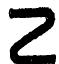
\includegraphics[keepaspectratio]{images/part001_40fd7be3.jpg}}

X 到 \(X'\) 上的等距映射当然是 X 的一致结构（相应地，拓扑）到 \(X'\) 的一致结构（相应地，拓扑）上的同构；这些命题的逆命题不成立，互不相同的等价度量的存在性（ \(\S\) 1，第 2 号）就表明了这一点。

设 X 是一个度量空间，d 是 X 上的度量。对每个 a \textgreater{} 0 ，用 \(V_{a}\) 表示 \(X \times X\) 的由所有点对 \((x, y)\) （满足 \(d(x, y) < a\) ）组成的子集，用 \(W_{a}\) 表示 \(X \times X\) 的由所有点对 \((x, y)\) （满足 \(d(x, y) \leqslant a\) ）组成的子集。当 a 取遍所有实数 \textgreater{} 0 组成的集（或仅仅取遍一个趋于 0 的 \textgreater{} 0 数列）时，诸集 \(V_{a}\) （相应地，\(W_{a}\) ）构成 X 的一致结构的开（相应地，闭）围域的一个基本系，这是由 d 的连续性得到的（§ 1，第 3 号）。我们有 \(\overline{V}_{a} \subset W_{a}\) ，但这两个集未必相同。

与 \(R^{n}\) 上欧氏距离的情形类比，集 \(\mathrm{V}_{a}(x)\) {[}相应地，\(\mathrm{W}_{a}(x)\) {]}称为以 x 为中心、以 a 为半径的开球（相应地，闭球）；它是 X 中的一个开（相应地，闭）集。又，由所有点 \(y \in X\) （满足 \(d(x, y) = a\) ）组成的集称为以 x 为中心、以 a 为半径的球面；它是一个闭集。由上所述，当 a 取遍所有实数 \textgreater0 组成的集或一个趋于 o 的 \textgreater0 数列时，以 x 为中心、以 a 为半径的开球（相应地，闭球）构成 x 的一个基本邻域系。

\pandocbounded{
\includegraphics[keepaspectratio]{images/part001_d95d2d33.jpg}}

读者应当警惕，不要以为任意度量空间中的球与球面具有第六章，§ 2 中所研究的欧氏球与球面同样的性质。例如，开球的闭包未必是同一中心、同一半径的闭球；闭球的边界未必是同一中心、同一半径的球面；开球（或闭球）未必连通；而且球面可以是空集（参看习题 4）。

设 A 与 B 是度量空间 X 的任意两个非空子集。数

\[
d (\mathbf {A}, \mathbf {B}) = \inf _ {x \in \mathbf {A}, y \in \mathbf {B}} d (x, y)
\]

称为集合 A 与 B 之间的距离。特别地，我们用 \(d(x, \mathbf{A})\) 表示集合 \(\{x\}\) 与集合 A 之间的距离；它称为点 x 到集合 A 的距离。于是

\[
d (x, \mathrm{A}) = \inf _ {y \in \mathrm{A}} d (x, y)
\]

由此得

\[
d (\mathbf {A}, \mathbf {B}) = \inf _ {x \in \mathbf {A}} d (x, \mathbf {B})
\]

（第四章，§ 5，第 4 号，命题 9）。

注。若 \(d(x, \mathrm{A}) = a\) ，可能发生 A 中没有到 \(x\) 的距离等于 \(a\) 的点的情形。然而，若 A 是紧的，这种情形绝不会出现，因为这时魏尔斯特拉斯定理（第四章，§6，第 1 号，定理 1）表明，存在 \(y \in \mathrm{A}\) 使得 \(d(x, \mathrm{A}) = d(x, y)\) 。

命题 2. \(d(x, \mathbf{A}) = 0\) 与 \(x \in \overline{\mathbf{A}}\) 这两个陈述等价。

因为 \(d(x, \mathbf{A}) = 0\) 表明：球 \(\mathbf{V}_a(x)\) 与 \(\mathbf{A}\) 相交，无论 \(a > 0\) 取何值；而这等价于 \(x \in \overline{\mathbf{A}}\) 。

命题 3. 函数 \(d(x, \mathbf{A})\) 在 \(\mathbf{X}\) 上一致连续。

设 \(x\) 与 \(y\) 是 \(\mathbf{X}\) 中任意两点；则对任意给定的 \(\varepsilon > 0\) ，存在 \(z \in \mathbf{A}\) 使得 \(d(y, z) \leqslant d(y, \mathbf{A}) + \varepsilon\) ，因而

\[
d (x, z) \leqslant d (x, y) + d (y, z) \leqslant d (x, y) + d (y, A) + \varepsilon
\]

由三角不等式。

更有 \(d(x, \mathbf{A}) \leqslant d(x, y) + d(y, \mathbf{A}) + \varepsilon\) ，且由于 \(\varepsilon\) 是任意的，由此得 \(d(x, \mathbf{A}) \leqslant d(x, y) + d(y, \mathbf{A})\) 。类似地有

\[
d (y, \mathbf {A}) \leqslant d (x, y) + d (x, \mathbf {A}),
\]

从而

\[
\left| d (x, \mathbf {A}) - d (y, \mathbf {A}) \right| \leqslant d (x, y),\tag{2}
\]

由此即得结论。

注。可以有 \(d(\mathbf{A}, \mathbf{B}) = 0\) ，对某两个子集 \(\mathbf{A}, \mathbf{B}\) （\(\mathbf{X}\) 的子集）而言，它们满足 \(\overline{\mathbf{A}} \cap \overline{\mathbf{B}} = \emptyset\) ，只要这两个子集都不由单独一个点组成。例如，在实直线 \(\mathbf{R}\) 上，整数 \(> 0\) 组成的集与序列 \((n + 1/2n)_{n \geqslant 1}\) 的点组成的集是两个互不相交的闭集，它们之间的距离为零。

然而，若 A 紧且 B 闭，则关系 \(d(A, B) = 0\) 蕴含 \(A \cap B \neq \varnothing\) ，因为借助关系式

\[
d (\mathbf {A}, \mathbf {B}) = \inf _ {x \in \mathbf {A}} d (x, \mathbf {B})
\]

由命题 3 与魏尔斯特拉斯定理可知，存在 \(x_0 \in \mathbf{A}\) 使得 \(d(x_0, \mathbf{B}) = d(\mathbf{A}, \mathbf{B}) = 0\) ，从而（命题 2）\(x_0 \in \mathbf{B}\) 。

X 的非空子集 A 的直径是数（有限或等于 +∞）

\[
\delta (\mathbf {A}) = \sup _ {x \in \mathbf {A}, y \in \mathbf {A}} d (x, y).
\]

``W \(_{a}\) -小集''（第二章，§ 3，第 1 号）的概念与直径 \(\leqslant a\) 的集的概念相同。非空集 A 由单独一个点组成的必要充分条件是 \(\delta(\mathbf{A}) = 0\) 。

X 的子集 A （关于度量 d）称为有界的，如果它的直径有限；等价地，如果对每个点 \(x_{0} \in X\) ，A 都包含在以 \(x_{0}\) 为中心的一个球中。有界集的每个子集是有界的，且有限个有界集的并是有界集。

注意，X 的一个子集可以关于度量 d 有界，而关于与 d 等价的某个度量无界（参看 § 1，第 2 号）。

\subsection{函数的振幅}

与直径的概念相关的是函数 \(f\) （定义在任意集合 \(\mathbf{X}\) 上、取值于度量空间 \(\mathbf{X}'\) 中）的振幅的概念；若 \(\mathbf{A}\) 是 \(\mathbf{X}\) 的任意非空子集，则直径 \(\delta(f(\mathbf{A}))\) 称为 \(f\) 在 \(\mathbf{A}\) 中的振幅。

此外，若 \(\mathbf{X}\) 是拓扑空间 \(\mathbf{Y}\) 的子集，且 \(x \in \overline{\mathbf{X}}\) ，则数

\[
\omega (x; f) = \inf \delta (f (\mathbf {V} \cap \mathbf {X}))
\]

（当 V 取遍 \(x\) 在 Y 中的邻域滤子时）称为 \(f\) 在 \(x \in \overline{\mathbf{X}}\) 处的振幅。

命题 4. 振幅 \(\omega(x; f)\) ——任意函数 \(f\) （定义在拓扑空间 Y 的子集 X 上、取值于度量空间 \(\mathbf{X}'\) 中）的振幅—— 在 \(\overline{\mathbf{X}}\) 上是上半连续的。

设 \(a\) 是 \(\overline{\mathbf{X}}\) 中任意一点；则对每个 \(k > \omega(a; f)\) ，存在一个开邻域 \(\mathbf{V}\) （ \(a\) 的），使得 \(\delta(f(\mathbf{V} \cap \mathbf{X})) \leqslant k\) ；对每个 \(x \in \mathbf{V} \cap \overline{\mathbf{X}}\) ，\(\mathbf{V}\) 是 \(x\) 的一个邻域，因而

\[
\omega (x; f) \leqslant \delta (f (\mathbf {V} \cap \mathbf {X})) \leqslant k,
\]

这表明 \(\omega\) 在点 a 处上半连续。

为使 \(\omega(x; f) = 0\) 在点 \(x \in \overline{\mathbf{X}}\) 处成立，必要且充分的是：对每个 \(\varepsilon > 0\) ，存在一个邻域 \(\mathbf{V}\) （ \(x\) 的），使得 \(f(\mathbf{V} \cap \mathbf{X})\) 包含在半径为 \(\varepsilon\) 的一个球中；若 \(x \in \mathbf{X}\) ，这个条件表明 \(f\) 在点 \(x\) 处（关于 \(\mathbf{X}\) ）连续；若 \(x \in \overline{\mathbf{X}} \cap \complement \mathbf{X}\) ，则 \(f\) 映 \(\mathbf{X}\) 上的一个滤子基 —— \(x\) 在 \(\mathbf{Y}\) 中的邻域滤子的迹 —— 为 \(\mathbf{X}'\) 上的一个柯西滤子基；特别地：

命题 5. 设 \(f\) 是定义在一个子集 \(\mathbf{X}\) （拓扑空间 \(\mathbf{Y}\) 的子集）上、取值于完备度量空间 \(\mathbf{X}'\) 中的函数。则 \(f\) 关于 \(\mathbf{X}\) 在点 \(x \in \overline{\mathbf{X}}\) 处有极限的必要充分条件是 \(f\) 在 \(x\) 处的振幅为零。

\subsection{可度量化一致空间}

定义 2. 集合 X 上的度量称为与 X 上的一致结构 U 相容，如果由该度量定义的一致结构与 U 重合。

集合 X 上的一致结构称为可度量化的，如果存在 X 上的一个度量与这个一致结构相容。一致空间称为可度量化的，如果它的一致结构可度量化。

不同的度量可以与同一个一致结构相容；这时它们是等价的（§ 1，第 2 号，定义 2）。

定理 1. 一致结构可度量化的必要充分条件是：它是豪斯多夫的，且该一致结构的围域滤子具有可数基。

该条件是必要的，因为（用第 2 号的记号）围域 \(V_{1/n}\) （ \(n \geqslant 1\) ）构成度量空间的一致结构的围域滤子的一个基。

该条件是充分的，因为若该条件满足，则由第 1 节，第 4 号的命题 2，所考察的一致结构由单个伪度量定义；由于该一致结构是豪斯多夫的，这个伪度量是度量。

推论 1. 由可数族伪度量定义的豪斯多夫一致结构是可度量化的。

因为若 \((f_n)\) 是定义这样一个结构的伪度量序列，则围域滤子由集的可数族 \(\overline{f}_n^1([0, 1/m])\) 生成，其中 \(m\) 与 \(n\) 都取遍整数 \(>0\) 组成的集。

推论 2. 可度量化一致空间的每个可数乘积都是可度量化的。

因为这样的空间是豪斯多夫的，且它的一致结构具有可数的围域基本系（第二章，§ 2，第 6 号）。

\subsection{可度量化拓扑空间}

定义 3. 集合 X 上的度量称为与 X 上的拓扑 C 相容，如果由该度量定义的拓扑与 C 重合。拓扑空间称为可度量化的，如果存在 X 上的一个度量与 X 的拓扑相容。

\pandocbounded{
\includegraphics[keepaspectratio]{images/part001_d7e316f7.jpg}}

集合 X 上都与同一个拓扑 \(\mathfrak{C}\) 相容的两个度量可以不等价。

R 的子空间 \(R_{+}^{*}\) 提供了这样的一个例子。由 R 的加法一致结构诱导的一致结构与由 \(R^{*}\) 的乘法一致结构诱导的一致结构都是可度量化的，并且都与 \(R_{+}^{*}\) 的拓扑相容；但它们不可比较。

我们还指出，可以存在与可度量化拓扑空间的拓扑相容的不可度量化的一致结构（习题 7）。

这里我们只满足于给出拓扑空间可度量化的必要条件（关于必要充分条件，参看第 4 节，习题 22）。首先，一个空间除非是完全正则的，否则不可能是可度量化的（事实上我们将在第 4 节，第 1 号，命题 2 中看到，可度量化空间必然是``正规''的，这是一个更强的条件）。另一方面，定理 1 表明：

命题 6. 可度量化空间的每个点都具有可数的基本邻域系。

更一般地：

命题 7. 在可度量化空间中，每个闭集都是可数个开集之交，每个开集都是可数个闭集之并。

设 \(d\) 是与可度量化空间 \(\mathbf{X}\) 的拓扑相容的一个度量。若 \(\mathbf{A}\) 是 \(\mathbf{X}\) 的闭子集，则它是诸开集 \(\mathrm{V}_{1/n}(\mathbf{A})\) {[}由所有点 \(x\in\mathbf{X}\) （满足 \(d(x,\mathbf{A})<\mathbf{1}/n\) ）组成的集；参看命题 2{]}之交。命题的第二部分通过取余集得到。

注。1) 这些必要条件不是充分的（参看习题 13）。2) 存在这样的空间：其中每个点都有可数的基本邻域系，但其中存在不是可数个开集之交的闭集（习题 15）；这样的空间不是可度量化的。

第 4 节定理 1 的推论 2 表明，可度量化拓扑空间的可数乘积是可度量化的。此外，可度量化空间的任意族 \((\mathbf{X}_t)_{t \in \mathbf{I}}\) 的和 X （第一章，§ 2，第 4 号）也是可度量化的。因为若 \(d_t\) 是与 \(\mathbf{X}_t\) 的拓扑相容的度量（对每个 \(t \in \mathbf{I}\) ），则我们可以假定 \(d_t\) 有界且 \(\mathbf{X}_t\) 的直径 \(\leqslant t\) ；于是可以定义一个距离 \(d\) （与 \(\mathbf{X}\) 的拓扑相容）：规定 \(d(x, y) = d_t(x, y)\) 当 \(x\) 与 \(y\) 都属于同一个 \(\mathbf{X}_t\) 时，否则规定 \(d(x, y) = t\) 。

\subsection{可数序列的使用}

命题 6 是可度量化空间理论中点的可数序列所起作用的根源；对许多问题而言，可以用它们来有效地代替滤子。这是因为可度量化空间中点的邻域滤子（从而还有收敛滤子）由该空间中点的收敛序列确定：因为由于一点的邻域滤子具有可数基，它是比它细的诸基本滤子之交（第一章，§ 6，第 8 号，命题 11），即与收敛到所考察点的诸序列相伴随的基本滤子之交。

另一方面，收敛序列的概念不适用于研究这样的拓扑空间：其中有些点的邻域滤子没有可数基。特别地，可以构造非离散的豪斯多夫拓扑空间，使得在每个点 x 处，x 的邻域的任意可数族之交仍是 \(x (*)\) 的邻域；在这样的空间中，仅有的收敛序列是那些从某个指标起各项都相等的序列。

作为使用可数序列的例子，我们给出下列命题：

命题 8. 在可度量化空间 X 中，点 x 属于 X 的非空子集 A 的闭包，其必要充分条件是存在 A 的一个收敛到 x 的点列。

由第一章，§ 7，第 3 号我们已知该条件是充分的。为看出它是必要的，考察一个可数基本邻域系 \((\mathbf{V}_n)\) （ \(x\) 的），使得 \(\mathbf{V}_{n+1} \subset \mathbf{V}_n\) 对每个 \(n\) 成立。若 \(x\) 属于 A 的闭包，则每个 \(\mathbf{V}_n\) 与 A 相交，且若 \(x_n\) 属于 \(\mathbf{V}_n \cap \mathbf{A}\) ，则序列 \((x_n)\) 收敛到 \(x\) (**)。

由命题 8 我们推出：

命题 9. 度量空间 X 完备的必要充分条件是 X 中每个柯西序列都收敛。

设 \(\hat{\mathbf{X}}\) 是 \(\mathbf{X}\) 的完备化。若存在一点 \(x \in \hat{\mathbf{X}}\) 不属于 \(\mathbf{X}\) ，则存在一个序列 \((x_n)\) （\(\mathbf{X}\) 中的点的序列），它收敛到 \(x\) ，而这是 \(\mathbf{X}\) 中一个不收敛的柯西序列。

命题 10. 设 X 是可度量化空间，f 是 X 到拓扑空间 \(X'\) 中的一个映射。则 f 在点 \(x \in X\) 处连续的必要充分条件是：只要 \((x_n)\) 是 X 中收敛到 x 的点列，序列 \((f(x_n))\) 就收敛到 \(f(x)\) （在 \(X'\) 中）。

该条件是必要的，这由第一章，§ 7，第 4 号，命题 9 的推论 1 得到。为证明它是充分的，考察邻域滤子 \(\mathfrak{B}'\) —— \(f(a)\) 在 \(\mathbf{X}'\) 中的邻域滤子；假设蕴含 \(\overline{f}(\mathfrak{B}')\) 粗于与每个收敛到 \(a\) 的序列相伴随的基本滤子，也就是说粗于每个收敛到 \(a\) 的基本滤子；而这些滤子之交是 \(a\) 的邻域滤子（第一章，§ 6，第 8 号，命题 11）。由此即得结论。

注意，命题 8 与命题 10 在每个点都具有可数基本邻域系的任何空间 X 中都成立。

\subsection{可度量化空间上的半连续函数}

命题 11. 设 X 是可度量化空间，f 是 X 上取值于闭区间 \([a, b]\) （ \(\overline{R}\) 中的闭区间）的下半连续函数。则 f 是 X 上取值于 \([a, b]\) 中的连续函数组成的递增序列的上包络。

由结构转移，我们可以假定 \(a = 0\) 且 \(b = 1\) 。

\begin{enumerate}
\def\labelenumi{(\roman{enumi})}
\tightlist
\item
  先设 \(f = \varphi_{\mathbf{A}}\) ，其中 \(\mathbf{A}\) 是 \(\mathbf{X}\) 的一个开子集。则函数 \(g_n\) —— 由 \(g_n(x) = n\) . inf \((d(x, \mathbf{X} - \mathbf{A}), \mathfrak{r}/n)\) 定义 —— 连续且 \(\geqslant 0\) （在 \(\mathbf{X}\) 上）；而且 \(g_n(x) = f(x)\) 当 \(x \in \mathbf{X} - \mathbf{A}\) 以及当
\end{enumerate}

\[
d (x, \mathbf {X} - \mathbf {A}) \geqslant \mathrm{r} / n.
\]

时也成立。由此立即可得 \(f = \sup_{n}(g_n)\) 。

\begin{enumerate}
\def\labelenumi{(\roman{enumi})}
\setcounter{enumi}{1}
\tightlist
\item
  一般情形，对每个整数 \(n \geqslant 1\) ，考察开集的有限递减序列
\end{enumerate}

\[
\mathrm{A} _ {k} = \overline {{{f}}} ^ {1} \left(\right] \frac {k}{n}, + \infty [) \quad (0 \leqslant k \leqslant n - 1);
\]

函数 \(g_{n} = \frac{1}{n}\sum_{k=1}^{n-1}\varphi_{\mathbf{A}_k}\) 是下半连续的，且 \(0 \leqslant f(x) - g_{n}(x) \leqslant 1/n\) 对一切 \(n\) 成立；因而 \(f\) 是序列 \((g_n)\) 的上包络。另一方面，\(g_{n}\) 是有限多个开集的特征函数的具正系数的线性组合，因而它是可数序列 \((h_{mn})_{m \geqslant 0}\) （由连续函数 \(\geqslant 0\) 组成的序列）的上包络（由 (i)）；故 \(f = \sup_{m,n} h_{mn}\) 。若令 \(f_{n} = \sup_{p \leqslant n, q \leqslant n} h_{pq}\) ，则我们看到序列 \((f_n)\) 是连续函数 \(\geqslant 0\) 的一个递增序列，以 \(f\) 为上包络，且不取值 \(1\) ，因为 \(g_{n} \leqslant n - 1/n\) 。

\subsection{可数型可度量化空间}

定义 4. 可度量化空间称为可数型的（或可分的），如果它的拓扑具有可数基。

显然，可数型可度量化空间的每个子空间仍是可数型的。乘积空间拓扑基的定义（第一章，§ 4，第 1 号）与第 4 号定理 1 的推论 2 表明，可数个可数型可度量化空间的乘积是可数型可度量化空间。同样，可数个可数型可度量化空间的和是可数型可度量化空间（第 5 号）。

命题 12. 若 X 是可度量化拓扑空间，则下列陈述等价：

\begin{enumerate}
\def\labelenumi{\alph{enumi})}
\item
  X 是可数型的。
\item
  X 有可数稠密子集。
\item
  X 同胚于方体 IN 的一个子空间，其中 I 是 R 中的区间 {[}o, i{]} 。
\end{enumerate}

由前面的注记，显然 c) 蕴含 a)；a) 蕴含 b)，因为若 \((\mathbf{U}_{n})\) 是 X 的拓扑的一个可数基，且 \(a_{n}\) 是 \(U_{n}\) 的一个点，则诸 \(a_{n}\) 构成 X 的一个稠密子集。最后证明 b) 蕴含 c)。设 \((a_{n})\) 是 X 的点的稠密序列，且对每个 \(x \in X\) ，令 \(\varphi(x)\) 为点 \((d(x, a_{n}))_{n \in \mathbb{N}}\) —— \(I^{N}\) 的点 ——（d 是与 X 的拓扑相容、且关于它 X 的直径 \(\leqslant 1\) 的一个度量）。我们将证明 \(\varphi\) 是 X 到 \(I^{N}\) 的一个子空间上的同胚。事实上，\(\varphi\) 是连续的，因为每个函数 \(x \to d(x, a_{n})\) 都连续；且 \(\varphi\) 是单射，因为 X 的每个点都是 \((a_{n})\) 的某个子序列的极限（命题 8）。设 B 是 X 中以 \(x_{0}\) 为中心、以 r 为半径的一个球，并设 n 是使

\[
\left| d (x _ {0}, a _ {n}) <   \frac {1}{3} r. \right|
\]

\(\varphi\) 把集 \(W\) —— 由满足以下条件的点 \(x\in X\) 组成的集 ——

\[
\left| d (x _ {0}, a _ {n}) - d (x, a _ {n}) \right| <   \frac {1}{3} r
\]

映为按定义是 \(\varphi(x_0)\) 在 \(\varphi(\mathbf{X})\) 中的一个邻域。但对每个 \(x \in W\) 有 \(d(x, a_n) < d(x_0, a_n) + \frac{1}{3} r < \frac{2}{3} r\) ，由此得

\[
d (x, x _ {0}) \leqslant d (x _ {0}, a _ {n}) + d (x, a _ {n}) <   r,
\]

这表明 W 是包含在 B 中的 \(x_{0}\) 的一个邻域，因而 \(\varphi\) 是 X 到 \(\varphi(\mathbf{X})\) 上的一个同胚。

\pandocbounded{
\includegraphics[keepaspectratio]{images/part001_a8399183.jpg}}

注意，对任意拓扑空间 X 而言，性质 b) 不一定蕴含可数基的存在性，即使 X 是紧的且 X 的每个点都有可数的基本邻域系（习题 13；参看第一章，§ 1，习题 7）。

命题 13. 设 X 是具有可数基 \((\mathbf{U}_n)\) 的拓扑空间；则对 X 的每个开覆盖 \((\mathbf{V}_t)_{i \in \mathbf{I}}\) ，存在 I 的可数子集 J，使得 \((\mathbf{V}_t)_{i \in \mathbf{J}}\) 是 X 的一个覆盖。

设 H 是由使 \(U_{n}\) 至少包含在某个 \(V_{t}\) 中的指标 n 组成的 N 的子集；序列 \((\mathrm{U}_{n})_{n\in\mathbf{H}}\) 是 X 的一个覆盖，因为每个点 \(x\in X\) 属于某个 \(V_{t}\) ，且由于 \(V_{t}\) 是开的，存在指标 n 使得 \(x\in U_{n}\subset V_{t}\) 。因而存在 H 到 I 中的一个映射 \(\psi\) ，使得 \(U_{n}\subset V_{\psi(n)}\) 对每个 \(n\in H\) 成立；取 \(J=\psi(H)\) ，它是可数的，命题得证。

\subsection{紧度量空间；紧可度量化空间}

一致空间预紧性的判别法（第二章，§ 4，第 2 号，定理 3）对度量空间给出下述命题：

命题 14. 度量空间 X 预紧的必要充分条件是：对每个 \(\varepsilon > 0\) ，存在 X 的由直径 \(\leqslant \varepsilon\) 的集组成的有限覆盖。

若再加上 X 完备这一假设，我们就得到度量空间紧性的一个判别法。

由命题 14 我们得到一个适用于可度量化空间的紧性拓扑判别法：

命题 15. 可度量化拓扑空间 X 紧的必要充分条件是：X 的每个无穷点列在 X 中有一个聚点。

第一章，§ 9，第 1 号的公理 (C) 表明该条件是必要的。为证明充分性，设 \(d\) 是与 \(\mathbf{X}\) 的拓扑相容的一个度量。我们先证明这样定义的度量空间 \(\mathbf{X}\) 是完备的：\(\mathbf{X}\) 中每个柯西序列都有聚点，从而是收敛的（第二章，§ 3，第 2 号，命题 5 的推论 2）；因而由命题 9，\(\mathbf{X}\) 是完备的。其次我们证明 \(\mathbf{X}\) 是预紧的；若非如此，则由命题 14，存在实数 \(\alpha > 0\) ，使得 \(\mathbf{X}\) 不能被 \(\mathbf{X}\) 的任何有限多个直径 \(\leqslant \alpha\) 的子集覆盖。于是我们可以对 \(n\) 用归纳法定义一个无穷序列 \((x_n)\) （\(\mathbf{X}\) 的点的序列），满足条件 \(d(x_p, x_n) > \frac{1}{2} \alpha\) 对一切 \(p < n\) 成立；而这样的序列不可能有聚点，因为每个半径 \(< \frac{1}{2} \alpha\) 的球至多包含该序列的一个点。

推论. 可度量化拓扑空间 X 的子集 A 相对紧的必要充分条件是：A 的每个无穷点列在 X 中有一个聚点。

设 \(d\) 是与 \(\mathbf{X}\) 的拓扑相容的一个度量。我们将应用命题 15 的判别法证明空间 \(\overline{\mathbf{A}}\) 是紧的。设 \((x_{n})\) 是 \(\overline{\mathbf{A}}\) 的点的一个序列；则对每个指标 \(n\) 存在 \(y_{n} \in \mathbf{A}\) 使得 \(d(x_{n}, y_{n}) < 1/n\) ；由假设，序列 \((y_{n})\) 有一个聚点 \(a \in \mathbf{X}\) ，且 \(a\) 也是序列 \((x_{n})\) 的聚点，因为若 \(y_{m}\) 位于以 \(a\) 为中心、以 \(1/n\) 为半径的球中（对某个 \(m > n\) ），则 \(x_{m}\) 位于以 \(a\) 为中心、以 \(2/n\) 为半径的球中。

应当指出，命题 15 并不是 X 的每个点处可数基本邻域系存在性的推论；存在不可度量化的、非紧的空间的例子，其中每个点都有可数的基本邻域系，且每个无穷点列都有聚点（习题 15）。

命题 16. 紧空间 X 可度量化的必要充分条件是它的拓扑具有可数基。

该条件是必要的。由命题 14，对每个整数 \(n \geqslant 1\) ，存在一个有限子集 \(A_n\) （\(X\) 的子集），使得 \(A_n\) 与 \(X\) 的每个点的距离 \(\leqslant 1/n\) ；因而可数集 \(A = \bigcup_{n} A_n\) 在 \(X\) 中稠密，于是由第 8 号的命题 12 即得结论。

该条件是充分的。设 \((\mathbf{U}_{n})\) 是 X 的拓扑的一个可数基。因而对角线 \(\Delta\) —— \(X \times X\) 的对角线 —— 的每个点的每个邻域都包含一个形如 \(U_{n} \times U_{n}\) 的邻域；对紧子集 \(\Delta\) （ \(X \times X\) 的紧子集）应用波莱尔–勒贝格公理可知，\(\Delta\) 的每个邻域都包含形如 \(U_{n} \times U_{n}\) 的集的一个有限并，而这样的并是 \(\Delta\) 的一个邻域。因而 \(\Delta\) 的这样的邻域——由形如 \(U_{n} \times U_{n}\) 的集的有限并组成的邻域——构成 X 的一致结构的一个围域基本系（第二章，§ 4，第 1 号，定理 1），于是由第 4 号的定理 1 即得结论。

推论. 设 X 是局部紧空间，X' 是通过给 X 添加一个无穷远点 ω 而得到的紧空间（第一章，§ 9，第 8 号）。则下列陈述等价：

\begin{enumerate}
\def\labelenumi{\alph{enumi})}
\item
  \(\mathbf{X}\) 的拓扑有可数基。
\item
  \(\mathbf{X}'\) 可度量化。
\item
  X 可度量化且是 \(\sigma\) -紧的。
\end{enumerate}

a) \(\Longrightarrow\) b)：设 \((\mathbf{U}_n)\) 是 \(\mathbf{X}\) 的拓扑的一个可数基。点 \(x \in \mathbf{X}\) 的每个邻域都包含 \(x\) 的一个紧邻域，而后者又包含 \(x\) 的一个等于某个 \(\mathbf{U}_n\) 的邻域。因而相对紧的诸 \(\mathbf{U}_n\) 构成 \(\mathbf{X}\) 的拓扑的一个基，于是我们可以假定所有 \(\mathbf{U}_n\) 都是相对紧的。因而 \(\mathbf{X}\) 是紧集 \(\overline{\mathbf{U}}_n\) 的可数并，即它是 \(\sigma\) -紧的；这蕴含在 \(\mathbf{X}'\) 中点 \(\omega\) 有由开邻域组成的可数基本系 \((\mathbf{V}_n)\) （第一章，§ 9，第 9 号，命题 15 的推论 2）。因而点 \(y \in \mathbf{X}'\) 的每个邻域都包含某个 \(\mathbf{U}_n\) 或某个 \(\mathbf{V}_n\) ，它是 \(y\) 的一个邻域，于是诸 \(U_{n}\) 与诸 \(V_{n}\) 构成 \(X'\) 的拓扑的一个可数基。因而由命题 16，\(X'\) 可度量化。

b) \(\Longrightarrow\) c): 若 \(X'\) 可度量化，则 \(\omega\) 有可数的基本邻域系，因而由第一章，§ 9，第 9 号，命题 15 的推论 2，\(X\) 是 \(\sigma\) -紧的。

c) \(\Longrightarrow a)\) ：由假设，存在相对紧开集的一个递增序列 \((\mathbf{V}_n)\) ，它们覆盖 \(\mathbf{X}\) 且满足 \(\overline{\mathbf{V}}_n \subset \mathbf{V}_{n+1}\) （第一章，§ 9，第 9 号，命题 15）。子空间 \(\overline{\mathbf{V}}_n\) 紧且可度量化，因而具有可数基（命题 16），从而 \(\mathbf{V}_n\) 也具有可数基。设 \((\mathbf{U}_{mn})_{m \geqslant 1}\) 是 \(\mathbf{V}_n\) 的拓扑的一个基。对每个 \(x \in \mathbf{X}\) 与每个邻域 \(W\) （ \(x\) 的），存在 \(n\) 使得 \(x \in \mathbf{V}_n\) ，因而存在 \(m\) 使得 \(x \in \mathbf{U}_{mn} \subset \mathbf{V}_n \cap W\) 。因而诸集 \(\mathbf{U}_{mn}\) （ \(m \geqslant 1\) ， \(n \geqslant 1\) ）构成 \(\mathbf{X}\) 的拓扑的一个基。

\subsection{可度量化空间的商空间}

若 X 是可度量化空间，R 是 X 上的一个等价关系，则商空间 X/R 未必可度量化（即使 X 局部紧 * 且 X/R 正规 * 也是如此）。然而：

命题 17. 紧可度量化空间的每个豪斯多夫商空间都是紧且可度量化的。

等价地，若 \(f\) 是紧可度量化空间 \(\mathbf{X}\) 到豪斯多夫空间 \(\mathbf{X}'\) 中的连续映射，则 \(f(\mathbf{X})\) 是 \(\mathbf{X}'\) 的可度量化子空间（第 I 章，§ 9，第 4 号，定理 2 的推论 4）。

设 \(\mathbf{X}\) 是紧可度量化空间，\(\mathbf{R}\) 是 \(\mathbf{X}\) 上的一个使 \(\mathbf{X} / \mathbf{R}\) 为豪斯多夫空间的等价关系。则 \(\mathbf{X} / \mathbf{R}\) 是紧的（第 I 章，§ 9，第 4 号，定理 2），故由命题 16，只需证明 \(\mathbf{X} / \mathbf{R}\) 的拓扑具有可数基。为此，我们要用到如下事实：\(\mathbf{R}\) 是闭的（第 I 章，§ 10，第 4 号，命题 8），并且模 \(\mathbf{R}\) 的各个等价类都是紧的。设 \(\varphi\) 是 \(\mathbf{X}\) 到 \(\mathbf{X} / \mathbf{R}\) 上的典范映射，\((\mathrm{U}_n)\) 是 \(\mathbf{X}\) 的拓扑的一个可数基。设 \(z\) 是 \(\mathbf{X} / \mathbf{R}\) 的任意一点，\(\mathbf{V}\) 是 \(z\) 在 \(\mathbf{X} / \mathbf{R}\) 中的一个邻域；则 \(\overline{\varphi}^1 (\mathbf{V})\) 是 \(\mathbf{X}\) 中紧集 \(\overline{\varphi}^1 (z)\) 的邻域。若 \(x\) 是 \(\overline{\varphi}^1 (z)\) 的任意一点，则存在一个集 \(\mathrm{U}_n\) ，它包含 \(x\) 且含于 \(\overline{\varphi}^1 (\mathrm{V})\) ；于是由波莱尔–勒贝格公理，存在一个有限开覆盖 \((\mathrm{U}_{n_k})_{1\leqslant k\leqslant r}\) ，它覆盖 \(\overline{\varphi}^1 (z)\) ，且使得：若以 \(\mathbf{W}\) 表示 \(\bigcup_{k}\mathrm{U}_{n_k},\mathrm{W}\) ，则它是 \(\overline{\varphi}^1 (z)\) 的一个含于 \(\overline{\varphi}^1 (\mathrm{V})\) 的邻域。由于 \(\mathbf{R}\) 是闭的，由此推出 \(\varphi (\mathbf{W})\) 是 \(z\) 在 \(\mathbf{X} / \mathbf{R}\) 中的一个含于 \(\mathbf{V}\) 的邻域（第 I 章，§ 5，第 4 号，命题 10）。设 \(\mathfrak{B}\) 表示形如 \(\varphi (\mathbf{W})\) 的集的内部所成的集，其中 \(\mathbf{W}\) 取遍集 \(\mathfrak{F}\) ，即形如 \(U_{n}\) 的集的一切有限并所成的集；这样我们便证明了 B 是 X/R 的拓扑的一个基，又因 F 是可数的，故 B 也是可数的。

命题 18. 设 X 是完备度量空间，R 是 X 上使 X/R 为豪斯多夫空间的开等价关系，\(\varphi: X \to X/R\) 是典范映射。则对 X/R 的任一紧子集 K，存在 X 的一个紧子集 \(K'\) 使 \(\varphi(K') = K\) 。

设 \(\mathfrak{B}_1\) 是 X 中以 \(1/2\) 为半径的全体开球所成的集。当 B 取遍 \(\mathfrak{B}_1\) 时，诸集 \(\varphi(B)\) 构成 K 的一个开覆盖，因此存在 X 的有限多个点 \(x_1, \ldots, x_m\) ，使得 \(\varphi\) 把以 \(1/2\) 为半径、以 \(x_i\) （ \(1 \leqslant i \leqslant m\) ）为中心的诸开球映为构成 K 的一个开覆盖的诸集。令 \(H_1 = \{x_1, \ldots, x_m\}\) ，并设已定义了有限集 \(H_i\) （ \(1 < i \leqslant n\) ），使得：

\begin{enumerate}
\def\labelenumi{(\roman{enumi})}
\item
  \(\mathbf{H}_i\subset \mathbf{H}_{i + 1}\) ，且 \(\mathbf{H}_{i + 1}\) 的每一点都以 \(<  \mathrm{I} / 2^{i}\) 的距离靠近 \(\mathbf{H}_i\) ，这里 \(\mathbf{I}\leqslant i\leqslant n - \mathbf{I};\)
\item
  \(\varphi\) 把以 \(1/2^i\) 为半径、以 \(\mathbf{H}_i\) 的点为中心的诸开球映为构成 \(\mathbf{K}\) 的开覆盖的诸开集，这里 \(1 \leqslant i \leqslant n\) 。
\end{enumerate}

设 \(\mathfrak{B}_{n+1}\) 是以 \(1/2^{n+1}\) 为半径、中心 \(x\) 满足 \(d(x, H_n) < 1/2^n\) （ \(d\) 为 X 上的度量）的全体开球所成的集。\(H_n\) 的性质表明，诸集 \(\varphi(B)\) （ \(B \in \mathfrak{B}_{n+1}\) ）构成 K 的开覆盖；因而存在有限集 \(L_{n+1} \subset X\) ，使得 \(\varphi\) 把以 \(1/2^{n+1}\) 为半径、中心属于 \(L_{n+1}\) 的诸开球映为构成 K 的一个开覆盖的诸集。取 \(H_{n+1} = H_n \cup L_{n+1}\) ，便知可以归纳地定义一个由 X 的有限子集组成的无限序列 \((H_n)\) ，它具有上述性质 (i) 与 (ii)。令 \(H = \bigcup_{n} H_n\) ，我们来证明 H 是预紧的。对每个 \(p > 0\) 及每点 \(z_{n+p} \in H_{n+p}\) ，存在点列 \(z_{n+i} \in H_{n+i}\) （ \(0 \leqslant i \leqslant p - 1\) ）使得

\[
d \left(z _ {n + i}, z _ {n + i + 1}\right) <   \mathrm{I} / 2 ^ {n + i} \quad \text { for } \quad \mathrm{o} \leqslant i \leqslant p - \mathrm{I};
\]

由此推出 \(d(z_n, z_{n+p}) \leqslant \sum_{i=0}^{p-1} \mathrm{I}/2^{n+i} \leqslant \mathrm{I}/2^{n-1}\) ，从而 \(d(y, \mathbf{H}_n) \leqslant \mathrm{I}/2^{n-1}\) 对一切 \(y \in \mathbf{H}\) 成立，这就证明了我们的断言。由于 \(\mathbf{X}\) 完备，\(\overline{\mathbf{H}}\) 是紧的，故 \(\varphi(\overline{\mathbf{H}})\) 是紧的。其次，我们证明 \(\mathbf{K} \subset \varphi(\overline{\mathbf{H}})\) 。若 \(z \in \mathbf{K}\) ，则按定义有 \(d(\overline{\mathbf{H}}_n, \overline{\varphi}^1(z)) \leqslant \mathrm{I}/2^n\) （对一切 \(n\) ），因而 \(d(\overline{\mathbf{H}}, \overline{\varphi}^1(z)) = 0\) ；但 \(\overline{\varphi}^1(z)\) 是闭集而 \(\overline{\mathbf{H}}\) 是紧集，故由此推出 \(\overline{\mathbf{H}} \cap \overline{\varphi}^1(z) \neq \emptyset\) （第 2 号，命题 3 后的注）；断言得证。于是，若 \(\mathbf{K}' = \overline{\mathbf{H}} \cap \overline{\varphi}^1(\mathbf{K})\) ，则 \(\mathbf{K}'\) 在 \(\overline{\mathbf{H}}\) 中闭，从而是紧的，并且由已证的结果有 \(\varphi(\mathbf{K}') = \mathbf{K}\) 。证毕。

\section{可度量化群、赋值域、赋范空间与赋范代数}

\subsection{可度量化拓扑群}

命题 1. 拓扑群 G 的左一致结构与右一致结构都可度量化，当且仅当 G 是豪斯多夫的且 G 的单位元 e 具有可数的基本邻域系。

该条件显然是必要的。反之，设它成立，令 \((\mathbf{V}_{n})\) 是 e 的一个基本邻域系；若以 \(U_{n}\) 表示诸对 \((x, y) \in \mathbf{G} \times \mathbf{G}\) 中满足 \(x^{-1}y \in V_{n}\) 者所成的集，则诸 \(U_{n}\) 构成 G 的左一致结构的一个可数围域基本系；由于此一致结构是豪斯多夫的，由 §2，第 4 号，定理 1 推出它是可度量化的。对 G 的右一致结构同理。

若拓扑群 G 的拓扑可度量化，则称 G 是可度量化的。于是命题 1 表明它的两个一致结构都是可度量化的。

借助下述概念，这一结果可以加强：

定义 1. 群 G（乘法记写）上的度量 d 称为左不变的（相应地，右不变的），如果我们有

\[
d (z x, z y) = d (x, y) \quad [ \text { resp. } d (x z, y z) = d (x, y) ]
\]

其中 \(x, y, z\) 取遍 \(\mathbf{G}\) 。

命题 2. 可度量化群 G 的左（相应地，右）一致结构可由 G 上的一个左不变（相应地，右不变）度量来定义。

设 e 的基本邻域系 \((\mathbf{V}_{n})\) 由对称邻域组成，使得 \(V_{n+1}^{3} \subset V_{n}\) 对每个 n 成立。~于是左一致结构的相应围域 \(U_{n}\) 是对称

的围域，且满足 \(\mathbf{U}_{n+1} \subset \mathbf{U}_n\) 。§1，第 4 号命题 2 的证明中所用的方法，使我们可以从围域序列 \((\mathbf{U}_n)\) 出发，构造出一个度量 \(d\) ，它定义在 \(\mathbf{G}\) 上且与 \(\mathbf{G}\) 的左一致结构相容；又因对每个 \(z \in \mathbf{G}\) ，映射 \((x, y) \to (zx, zy)\) 保持每个 \(\mathbf{U}_n\) 不变，由 \(d\) 的定义可知它是左不变度量。此方法对右一致结构同样适用。

注意，若 G 的两个一致结构不同，则度量 d 不是右不变的，因而一般地 \(d(x^{-1}, y^{-1}) \neq d(x, y)\) 。

特别地，若 G 是可度量化交换群，则它的一致结构由一个不变度量 d 定义；若 G 用加法记写，我们有

\[
d (x, y) = d (\mathrm{o}, y - x) = d (\mathrm{o}, x - y).
\]

我们常以 \(|x|\) （或 \(||x||\) ）表示 \(d(0, x)\) ；这时

\[
d (x, y) = | x - y |.
\]

函数 \(|x|\) 满足下列三个条件：

\begin{enumerate}
\def\labelenumi{\alph{enumi})}
\item
  \(|-x| = |x|\) 对一切 \(x \in G\) 成立。
\item
  \(|x + y| \leqslant |x| + |y|\) 对一切 \(x \in G\) 与一切 \(y \in G\) 成立。
\item
  \(|x| = 0\) 当且仅当 \(x = 0\) 。
\end{enumerate}

反之：

命题 3. 设 G 是用加法记写的交换群，\(x \to |x|\) 是满足上述条件 a)、b)、c) 的一个映射 \(\mathbf{G} \to \mathbf{R}_+\) 。则函数 \(d(x, y) = |x - y|\) 是 G 上的不变度量；它在 G 上定义的拓扑 C 与 G 的群结构相容，且由 d 定义的一致结构与赋有拓扑 C 的 G 所成拓扑群的一致结构相同。

函数 \(d(x, y)\) 是 \(G\) 上的度量，因为关系 \(d(x, y) = 0\) 等价于 \(x = y\) （由 \(c\) ）；而有 \(d(x, y) = d(y, x)\) （由 \(a\) ）；并且

\[
d (x, y) = | (x - z) + (z - y) | \leqslant | x - z | + | z - y | = d (x, z) + d (z, y)
\]

这是由 \(b\) ) 得到的。此外，\(d\) 是不变的，因为 \((x + z) - (y + z) = x - y\) 。对每个实数 \(\alpha > 0\) ，令 \(V_{\alpha}\) 为全体 \(x \in G\) 中满足 \(|x| < \alpha\) 者所成的集；则诸 \(V_{\alpha}\) 构成一个基本邻域系 \(\mathfrak{S}\) ，即 \(o\) 关于拓扑 \(\mathfrak{C}\) 的基本邻域系；又因 \(d\) 不变，\(a + \mathfrak{S}\) 是 \(a\) 的一个基本邻域系（关于拓扑 \(\mathfrak{C}\) ；这里 \(a \in G\) 任意）。由 \(a\) ，诸 \(V_{\alpha}\) 是对称的；由 \(b\) ，有 \(V_{\alpha} + V_{\alpha} \subset V_{2\alpha}\) ；因而拓扑 \(\mathfrak{C}\) 与 \(G\) 的群结构相容（第 III 章，§ 1，第 2 号）。命题的最后一部分立即可得。

条件 \(a), b)\) 与 \(c)\) 等价于 \(c)\) 连同条件

\[
| x - y | \leqslant | x | + | y |.\tag{\(b^{\prime}\)}
\]

因为 \(a)\) 与 \(b)\) 显然蕴含 \(b')\) ；反之，取 \(x = 0\) 代入 \(b')\) 并利用 \(c)\) ，得 \(|-y| \leqslant |y|\) ；把 \(y\) 换成 \(-y\) 便得 \(|-y| = |y|\) ，此即 \(a)\) ；再把 \(y\) 换成 \(-y\) 代入 \(b')\) 即得 \(b)\) 。

命题 4. 若 G 是可度量化群，则 G 的每个豪斯多夫商群 G/H 都可度量化。若 G 还是完备的，则 G/H 是完备的 (*)。

命题的第一部分是如下事实的推论：G/H 的单位元在 G/H 中具有可数的基本邻域系；因为若 \((\mathbf{V}_{n})\) 是 e 在 G 中的基本邻域系，则 \(\dot{V}_{n}\) （诸集 \(V_{n}\) 在 G/H 中的典范像）构成 G/H 的单位元的基本邻域系（第 III 章，§ 2，第 6 号，命题 17）。

要证明当 G 完备时 G/H 也完备，由 § 2，第 6 号，命题 9，只需证明每个柯西序列 \((\dot{x}_{n})\) （关于 G/H 的左一致结构）都收敛。必要时可代之以 \((\dot{x}_{n})\) 的子序列，从而可设对每对满足 \(p \geqslant n\) 且 \(q \geqslant n\) 的指标 p、q，有 \(\dot{x}_{p}^{-1}\dot{x}_{q} \in \dot{V}_{n}\) ；这表示对每对点 \(y \in \dot{x}_{p}, z \in \dot{x}_{q}\) ，有 \(y^{-1}z \in HV_{n} = V_{n}H\) ；因而对每个 \(y \in \dot{x}_{p}\) ，\(\dot{x}_{q}\) 与 y 的邻域 \(yV_{n}\) 之交非空。现设序列 \((V_{n})\) 已选得使 \(V_{n+1}^{2} \subset V_{n}\) ，并归纳地定义 G 中点的序列 \((x_{n})\) ，使得 \(x_{n} \in \dot{x}_{n}\) 且 \(x_{n+1} \in x_{n}V_{n}\) ；由前所述这是可能的。于是由归纳法推出，对每个 p \textgreater{} 0 有 \(x_{n+p} \in x_{n}V_{n}V_{n+1} \ldots V_{n+p-1} \subset x_{n}V_{n-1}\) 。因此序列 \((x_{n})\) 是 G 中的柯西序列，故收敛于一点 a；并且立即得出，a 在 G/H 中的典范像 \(\dot{a}\) 是序列 \((\dot{x}_{n})\) 的极限。

推论 1. 设 G 是完备可度量化群，\(G_{0}\) 是 G 的稠密子群，\(H_{0}\) 是 \(G_{0}\) 的闭正规子群。若 H 是 \(H_{0}\) 在 G 中的闭包，则商群 \(G_{0}/H_{0}\) 的完备化同构于 G/H。

H 是 G 的正规子群（第 III 章，§ 2，第 3 号，命题 8），且命题 4 表明 G/H 是完备的。又若 \(\varphi\) 是 G 到 G/H 上的典范映射，则显然 \(\varphi(G_0)\) 在 G/H 中稠密。因此结论由第 III 章，§ 2，第 7 号，命题 21 得出。

设 \(G, G'\) 是两个豪斯多夫交换拓扑群，\(\hat{G}, \hat{G}'\) 是它们各自的完备化。我们回忆（第 III 章，§ 3，第 3 号，命题 5）：若 \(u\) 是 \(G\) 到 \(G'\) 中的连续同态，则 \(u\) 一致连续，且可唯一扩张为 \(\hat{G}\) 到 \(\hat{G}'\) 中的连续同态 \(\hat{u}\) ，在以下

本小节的其余部分中即用此记号。图表

\pandocbounded{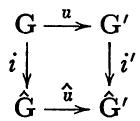
\includegraphics[keepaspectratio]{images/part001_945be03d.jpg}}

（其中 \(i\) ， \(i'\) 是典范单射）是交换的。若 \(v\) 是 \(\mathbf{G}'\) 到豪斯多夫交换拓扑群 \(\mathbf{G}''\) 中的连续同态，且 \(w = v \circ u\) ，则立即得出 \(\hat{w} = \hat{v} \circ \hat{u}\) 。

设 H 是 G 的闭子群，令 E = G/H。设 \(j: H \to G\) 与 \(p: G \to E\) 是典范映射。设 \(\overline{H}\) 是 H 在 \(\hat{G}\) 中的闭包；\(\overline{H}\) 是完备群，我们把它与 H 的完备化 \(\hat{H}\) 等同。j 的连续延拓 \(\hat{j}\) （到 \(\hat{H}\) 上）显然是 \(\hat{H}\) 到 \(\hat{G}\) 中的典范单射。

以下设 G 是可度量化的。于是 E = G/H 到 \(\hat{G}/\hat{H}\) 中的典范映射是 E 到完备群 \(\hat{G}/\hat{H}\) 的一个稠密子群上的拓扑同构（推论 1），从而我们可把 \(\hat{G}/\hat{H}\) 与 \(\hat{E}\) 等同，并把 p 的连续延拓 \(\hat{p}\) （到 \(\hat{G}\) 上）与 \(\hat{G}\) 到 \(\hat{G}/\hat{H}\) 上的典范映射等同。

推论 2. 设 G，G‘ 是两个可度量化交换拓扑群；u: G → G’ 是严格态射，其核为 N、像为 P。则 \(\hat{u} : \hat{G} \rightarrow \hat{G}'\) 是严格态射，其核为 \(\hat{N}\) 、像为 \(\hat{P}\) 。

设 \(u = j \circ v \circ p\) 是 \(u\) 的典范分解，其中 \(v\) 是拓扑群 \(G/N\) 到拓扑群 \(u(G) = P\) 上的同构。我们有 \(\hat{u} = \hat{j} \circ \hat{v} \circ \hat{p}\) ，并且已经看到 \(\hat{p}\) 是 \(\hat{G}\) 到 \(\hat{G}/\hat{N}\) 上的典范映射，而 \(\hat{j}\) 是 \(\hat{P}\) 到 \(\hat{G}'\) 中的典范映射。另一方面，\(\hat{v}\) 是 \(\hat{G}/\hat{N}\) 到 \(\hat{P}\) 上的同构（第 III 章，§ 3，第 4 号，命题 5），由此即得结论。

推论 3. 设 \(\mathbf{G}, \mathbf{G}'\) ， \(\mathbf{G}''\) 是三个可度量化交换拓扑群，\(u: \mathbf{G} \to \mathbf{G}'\) 与 \(v: \mathbf{G}' \to \mathbf{G}''\) 是两个严格态射，使得序列 \(\mathbf{G} \xrightarrow{u} \mathbf{G}' \xrightarrow{v} \mathbf{G}''\) 是正合的{[}即 \(u(\mathbf{G}) = \overline{v}^{1}(\mathbf{o})\) {]}。则序列 \(\hat{\mathbf{G}} \xrightarrow{\hat{u}} \hat{\mathbf{G}}' \xrightarrow{\hat{v}} \hat{\mathbf{G}}''\) 是正合的。

因为若令 \(\mathrm{N} = u(\mathrm{G}) = \overline{v}^{1}(\mathrm{o})\) ，则由推论 2，\(\hat{N}\) 既是 \(\hat{u}\) 的像又是 \(\hat{v}\) 的核。

注。1) 设 G 是非豪斯多夫拓扑群，但与之相伴的豪斯多夫群可度量化；等价地，G 的单位元在 G 中具有可数的基本邻域系。命题 4 的证明可不加修改地用于这一情形（H 为 G 的任意正规子群），它表明与 G/H 相伴的豪斯多夫群可度量化，并且只要 G 完备，G/H 就是完备群（一般不是豪斯多夫的）。

\begin{enumerate}
\def\labelenumi{\arabic{enumi})}
\setcounter{enumi}{1}
\tightlist
\item
  设 \(d\) 是定义可度量化群 G 的拓扑的左不变度量，H 是 G 的闭正规子群。若 \(\dot{x}\) 与 \(\dot{y}\) 是 G/H 的任意两点，考虑距离 \(d(\dot{x},\dot{y})\) ，即 G 中两个闭子集 \(\dot{x},\dot{y}\) 之间的距离（§ 2，第 2 号）；我们将看到，这个函数是 G/H 上的左不变度量，并且定义这个商群的拓扑。
\end{enumerate}

首先注意，若 \(x \in \dot{x}\) 且 \(y \in \dot{y}\) ，则有 \(d(\dot{x}, \dot{y}) = d(x, \mathrm{H}y)\) ；因为 \(d(x, \mathrm{H}y) = \inf_{h \in \mathbf{H}} d(x, h y)\) ，从而 \(d(h' x, \mathrm{H} y) = d(x, \mathrm{H} y)\) 对一切 \(h' \in \mathrm{H}\) 成立，因为 \(d\) 是左不变的；这就证明了断言（§ 2，第 2 号）。于是对每个 \(\dot{z} \in \mathrm{G} / \mathrm{H}\) 有{[}§ 2，第 2 号，公式 (2){]}

\[
\left| d (\dot {x}, \dot {z}) - d (\dot {y}, \dot {z}) \right| = \left| d (x, \dot {z}) - d (y, \dot {z}) \right| \leqslant d (x, y);
\]

又因这个不等式对一切 \(x \in \dot{x}\) 与一切 \(y \in \dot{y}\) 成立，我们有 \(|d(\dot{x}, \dot{z}) - d(\dot{y}, \dot{z})| \leqslant d(\dot{x}, \dot{y})\) ，这表明 \(d(\dot{x}, \dot{y})\) 是 G/H 上的度量。此外，对任意 \(z \in \dot{z}\) ，我们有

\[
d (\dot {z} \dot {x}, \dot {z} \dot {y}) = \inf _ {h \in \mathbf {H}} d (z x, h z y)
\]

这是由上面的式子得到的；但由于 \(hzy = z(z^{-1}hz)y\) ，并且 \(z^{-1}hz\) 随 \(h\) 取遍 H 而取遍 H（H 是正规的），\(d(x,y)\) 的左不变性表明有 \(d(zx, \mathrm{Hz}) = d(x, \mathrm{Hy}) = d(\dot{x}, \dot{y})\) 。最后，若 V 是 G 中 \(e\) 的由 \(d(e, x) < \alpha\) 定义的邻域，则 V 在 G/H 中的像 V 就是由 \(d(\dot{e}, \dot{x}) < \alpha\) 定义的集；这就完成了证明。

\subsection{赋值除环}

定义 2. 除环 K 上的绝对值是一个映射 \(x \to |x|\) ，它把 K 映入 \(\mathbf{R}_{+}\) ，且满足下列条件：

\((\mathbf{VM}_{\mathbf{I}})\) \(|x| = 0\) 当且仅当 \(x = 0\) 。

\((\mathbf{VM}_{\mathbf{II}})\quad |xy| = |x|.|y|\) 对一切 \(x,y\) （\(\mathbf{K}\) 中的）成立。

\((\mathbf{VM}_{\mathbf{III}})\quad |x + y|\leqslant |x| + |y|\) 对一切 \(x,y\) （\(\mathbf{K}\) 中的）成立。

由 \((\mathbf{VM}_{\mathbf{II}})\) 有 \(|x| = |\mathrm{I}|.|x|\) ，又由 \((\mathbf{VM}_{\mathbf{I}})\) 至少有一个 \(x\) 使 \(|x| \neq 0\) ，故 \(|\mathrm{I}| = \mathrm{I}\) ；由此推出 \(\mathrm{I} = |- \mathrm{I}|^2\) ，因此 \(|- \mathrm{I}| = \mathrm{I}\) ，从而

\[
| - x | = | - \mathrm{I} | | x | = | x |;
\]

因此 \(|x - y| \leqslant |x| + |y|\) 对一切 \(x, y\) （\(\mathbf{K}\) 中的）成立。于是我们可以说，\(d(x, y) = |x - y|\) 是加法群 \(\mathbf{K}\) 上的不变度量，并且映射 \(x \to |x|\) 是由 K 的非零元素组成的乘法群 \(K^{*}\) 到乘法群 \(R_{+}^{*}\) （由实数 \textgreater0 组成）中的同态。

不变度量 \(|x - y|\) 在 K 上定义了一个度量空间拓扑，它与 K 的加法群结构相容（第 1 号，命题 3）；而且，这一拓扑与 K 的除环结构相容。因为 xy 在 \(K \times K\) 上的连续性由关系式

\[
x y - x _ {0} y _ {0} = (x - x _ {0}) (y - y _ {0}) + (x - x _ {0}) y _ {0} + x _ {0} (y - y _ {0}),
\]

由此得到

\[
\left| x y - x _ {0} y _ {0} \right| \leqslant \left| x - x _ {0} \right|. \left| y - y _ {0} \right| + \left| x _ {0} \right|. \left| y - y _ {0} \right| + \left| y _ {0} \right|. \left| x - x _ {0} \right|.
\]

同样，\(x^{-1}\) 在每一点 \(x_{0} \neq 0\) 处的连续性由恒等式 \(x^{-1} - x_{0}^{-1} = x^{-1} (x_{0} - x)x_{0}^{-1}\) 得出，由 \((\mathrm{VM}_{\mathrm{II}})\) 它给出

\[
\left| x ^ {- 1} - x _ {0} ^ {- 1} \right| = \frac {\left| x - x _ {0} \right|}{\left| x _ {0} \right| . \left| x \right|};
\]

现若 \(\varepsilon > 0\) 满足 \(\varepsilon < |x_0|\) ，则关系 \(|x - x_0| \leqslant \varepsilon\) 蕴含 \(|x| \geqslant |x_0| - \varepsilon\) ，由此得 \(|x^{-1} - x_{0}^{-1}| \leqslant \varepsilon / |x_0| (|x_0| - \varepsilon)\) ；这就建立了 \(x^{-1}\) 在点 \(x_0\) 处的连续性。

定义 3. 赋值除环就是赋有由 K 上一个给定绝对值所定义之结构的除环 K。

赋值除环总被视为赋有由其绝对值定义的拓扑，这使它成为拓扑除环。若 \(K_{0}\) 是赋值除环 K 的一个子除环，则 K 上的绝对值在 \(K_{0}\) 上的限制是 \(K_{0}\) 上的一个绝对值，它在 \(K_{0}\) 上定义由 K 的拓扑诱导的拓扑。

例。1) 设 K 是任意除环。对每个 \(x \in \mathbf{K}\) ，令 \(|x| = \mathbf{i}\) （若 \(x \neq 0\) ），并令 \(|0| = 0\) 。如此定义的映射 \(x \to |x|\) 是 K 上的绝对值，称为平凡绝对值。除环 K 上由绝对值 \(|x|\) 定义的拓扑是离散的，当且仅当 \(|x|\) 是平凡绝对值。此条件显然是充分的；反之，若 K 的拓扑是离散的，则 \(|x|\) 不能取任何 \(\alpha > 0\) 的值，除非它是 \(\mathbf{i}\) ；因为若有 \(|x_0| = \alpha < \mathbf{i}\) ，则序列 \((x_0^n)\) 将由非零项组成且收敛于 \(\mathbf{o}\) ；要处理 \(\alpha > \mathbf{i}\) 的情形，就用 \(x_0^{-1}\) 代替 \(x_0\) 。

\begin{enumerate}
\def\labelenumi{\arabic{enumi})}
\setcounter{enumi}{1}
\item
  实数的绝对值（第 IV 章，§ 1，第 6 号）满足公理 \((\mathrm{VM}_{\mathrm{I}})\) ， \((\mathrm{VM}_{\mathrm{II}})\) 与 \((\mathrm{VM}_{\mathrm{III}})\) ，并且它在域 \(\mathbf{R}\) 上定义的拓扑就是实直线的拓扑。在复数域 \(\mathbf{C}\) （与 \(\mathbf{R}^2\) 等同）上{[}相应地，四元数体 \(\mathbf{H}\) （与 \(\mathbf{R}^4\) 等同）上{]}，欧氏范数同样是绝对值，并且定义域 C（相应地，除环 H）的拓扑（第 VIII 章，§ 1，第 2 号与第 4 号）。
\item
  在除环 K 上，实赋值是定义在 \(K^{*}\) 上、取值于 R 中的函数 v，它满足下列条件：a) 若 \(x \in K^{*}\) 且 \(y \in K^{*}\) ，则 \(v(xy) = v(x) + v(y)\) ；b) 若此外还有 \(x + y \neq 0\) ，则 \(v(x + y) \geqslant \inf(v(x), v(y))\) 。若 a 是任一实数 \textgreater1，则令 \(|x| = a^{-v(x)}\) （对 \(x \neq 0\) ），并令 \(|0| = 0\) ，便可在 K 上定义一个绝对值。因为关系式 \(v(xy) = v(x) + v(y)\) （对 \(x \neq 0\) 与 \(y \neq 0\) ）蕴含对这些 x、y 值的关系式 \(|xy| = |x|.|y|\) ，且当 x、y 之一为零时此关系平凡成立；同样，由关系式 \(v(x + y) \geqslant \inf(v(x), v(y))\) （当 \(x \neq 0\) 、 \(y \neq 0\) 且 \(x + y \neq 0\) 时）推出 \(|x + y| \leqslant \sup(|x|, |y|) \leqslant |x| + |y|\) ，并且当 x、y、 \(x + y\) 之一为零时这些不等式仍然成立。特别地，若 \(v_{p}(x)\) 是有理数域 Q 上的 p 进赋值（x 的素因子分解中 p 的指数），则相应的绝对值 \(|x|_{p} = p^{-v_{p}(x)}\) 称为域 Q 上的 p 进绝对值（参见第 III 章，§ 6，习题 23）。
\end{enumerate}

注。若 \(x\) 是赋值除环中的单位根，则 \(|x| = 1\) ，因为 \(x^n = 1\) 蕴含 \(|x|^n = 1\) ，从而 \(|x| = 1\) 。特别地，有限域上唯一的绝对值是平凡绝对值，因为这种域的每个元素 \(\neq 0\) 者都是单位根。

定义 4. 除环 K 上的两个绝对值称为等价的，如果它们在 K 上定义相同的拓扑。

命题 5. 两个绝对值 \(|x|_1, |x|_2\) （在除环 \(K\) 上，均非平凡绝对值）等价，当且仅当关系 \(|x|_1 < i\) 蕴含 \(|x|_2 < i\) 。这时存在实数 \(\rho > 0\) ，使得 \(|x|_2 = |x|_1^p\) 对一切 \(x \in K\) 成立。

此条件是必要的，因为全体 \(x \in \mathbf{K}\) 中满足 \(|x|_1 < 1\) 者所成的集，与全体 \(x\) 中关于由绝对值 \(|x|_1\) 定义的拓扑使 \(\lim x^n = 0\) 者所成的集相同。

反之，设 \(|x|_1 < \mathrm{i} \Longrightarrow |x|_2 < \mathrm{i}\) 。则有 \(|x|_1 > \mathrm{i} \Longrightarrow |x|_2 > \mathrm{i}\) ，因为 \(|x^{-1}|_1 < \mathrm{i}\) ，从而 \(|x^{-1}|_2 < \mathrm{i}\) 。由假设绝对值 \(|x|_1\) 不是平凡的，故存在 \(x_0 \in \mathbf{K}\) 使 \(|x_0|_1 > \mathrm{i}\) 。令 \(a = |x_0|_1\) ， \(b = |x_0|_2\) ，并令 \(\rho = \log b / \log a > 0\) 。设 \(x \in \mathbf{K}^*\) ，令 \(|x|_1 = |x_0|^{\gamma}\) 。若整数 \(m\) 与 \(n\) 满足 \(n > 0\) 且 \(m/n > \gamma\) ，则 \(|x|_1 < |x_0|_1^{m/n}\) ，因此 \(|x^n x_0^{-m}|_1 < \mathrm{i}\) ；于是 \(|x^n x_0^{-m}|_2 < \mathrm{i}\) ，即 \(|x|_2 < |x_0|_2^{m/n}\) 。类似地，若 \(m/n < \gamma\) ，则得 \(|x|_2 > |x_0|_2^{m/n}\) ；由此推出 \(|x|_2 = |x_0|_2^\gamma\) ；换言之

\[
\log | x | _ {2} = \gamma \log b = \gamma \rho \log a = \rho \log | x | _ {1},
\]

即 \(|x|_2 = |x|_1^p\) 。现在显然，在 \(\mathbf{K}\) 上由 \(|x|_1\) 与 \(|x|_2\) 定义的诸拓扑的零邻域是相同的。

反之，若 \(|x|\) 是 \(K\) 上任一绝对值，则函数 \(|x|^{\circ}\) 是 \(K\) 上的绝对值（与 \(|x|\) 等价），对一切 \(\rho\) （满足 \(0 < \rho \leqslant 1\) ）。只需验证不等式 \(|x + y|^{\circ} \leqslant |x|^{\circ} + |y|^{\circ}\) ；由于 \(|x + y|^{\circ} \leqslant (|x| + |y|)^{\circ}\) ，只需证明：若 \(a > 0\) 且 \(b > 0\) ，则 \((a + b)^{\circ} \leqslant a^{\circ} + b^{\circ}\) 对任何 \(\rho\) （满足 \(0 < \rho \leqslant 1\) ）成立。若令 \(c = a / (a + b)\) 与 \(d = b / (a + b)\) ，则有 \(c + d = 1\) ，待证的不等式为 \(c^{\circ} + d^{\circ} \geqslant 1\) ；但这由关系式 \(c^{\circ} \geqslant c\) 与 \(d^{\circ} \geqslant d\) 立即得出，它们当 \(0 < c \leqslant 1\) 、 \(0 < d \leqslant 1\) 、 \(0 < \rho \leqslant 1\) 时成立。

因此，r \textgreater{} 0 中使 \(|x|^{r}\) 成为绝对值的那些值的集合是 R 中以 o 为左端点的有限或无限区间；若它是有限的，则它显然是闭的；因为若 \(|x + y|^{r} \leqslant |x|^{r} + |y|^{r}\) 对 K 中任意 x、y 及一切满足 \(0 < r < r_{0}\) 的 r 成立，则由连续性该不等式对 \(r = r_{0}\) 仍成立。若 \(|x|^{r}\) 对一切 r \textgreater{} 0 都是绝对值，则我们有

\[
| x + y | \leqslant (| x | ^ {r} + | y | ^ {r}) ^ {1 / r}
\]

对一切 \(x\) 与 \(y\) （\(\mathbf{K}\) 中的）以及一切 \(r > 0\) 成立。现在，若 \(a, b\) 是两个实数 \(\geqslant 0\) ，则有 \(\lim_{r \to \infty} (a^r + b^r)^{1/c} = \sup (a, b)\) ；因为，例如设 \(a \geqslant b\) ，我们有 \(a \leqslant (a^r + b^r)^{1/r} \leqslant 2^{1/r} a\) ，令 \(r \to +\infty\) 即得结果。

于是，若 \(|x|^r\) 对一切 \(r > 0\) 是绝对值，则我们有

\[
| x + y | \leqslant \sup (| x |, | y |)
\]

这可以表述为：\(v(x) = -\log |x| (x \neq 0)\) 是 K 上的赋值。

注。命题 5 的证明表明：若由 \(|x|_2\) 定义的拓扑比由 \(|x|_1\) 定义的拓扑粗，且 \(|x|_1\) 不是平凡的，则 \(|x|_1\) 与 \(|x|_2\) 等价，因为这时关系 \(|x|_2 < 1\) 蕴含 \(|x|_2 < 1\) 。于是，\(K\) 上两个均非平凡的绝对值所定义的拓扑不能比较而不相同。

命题 6. 设 \(\hat{\mathbf{K}}\) 是除环 \(\mathbf{K}\) 赋有绝对值 \(|x|\) 后的完备化，则它是一个除环，且函数 \(|x|\) 可由连续性扩张为 \(\hat{\mathbf{K}}\) 上的绝对值，它定义 \(\hat{\mathbf{K}}\) 的拓扑。

设 \(\mathfrak{F}\) 是 K 上的柯西滤子（关于加法一致结构），它不以 o 为聚点；要证明 \(\hat{\mathbf{K}}\) 是除环，只需证明 \(\mathfrak{F}\) 在映射 \(x \to x^{-1}\) 下的像是柯西滤子基（第 III 章，§ 6，第 8 号，命题 7）。由假设，存在实数 \(\alpha > 0\) 与集 \(\mathrm{A} \in \mathfrak{F}\) ，使得 \(|x| \geqslant \alpha\) 对一切 \(x \in \mathrm{A}\) 成立；另一方面，对每个 \(\varepsilon > 0\) 存在集 \(\mathrm{B} \in \mathfrak{F}\) ，使得 \(\mathrm{B} \subset \mathrm{A}\) 且 \(|x - y| \leqslant \varepsilon\) 对一切 \(x \in \mathrm{B}\)

与 \(y\in \mathbf{B}\) 成立；由此

\[
\left| x ^ {- 1} - y ^ {- 1} \right| = \frac {\left| x - y \right|}{\left| x \right| . \left| y \right|} \leqslant \frac {\varepsilon}{\alpha^ {2}},
\]

这就得出命题的第一部分。不变度量 \(|x - y| = d(x, y)\) 由连续性扩张为 \(\hat{\mathbf{K}}\) 上的度量（§ 2，第 1 号，命题 1），它定义 \(\hat{\mathbf{K}}\) 的拓扑，且由恒等式延拓原理是不变的；我们仍以 \(d(x, y)\) 记这个不变度量。若令 \(|x| = d(0, x)\) （对 \(x \in \hat{\mathbf{K}}\) ），则显然 \(|x|\) 是函数 \(|x|\) （\(\mathbf{K}\) 上的）的连续延拓，从而由恒等式延拓原理是 \(\hat{\mathbf{K}}\) 上的绝对值。

\subsection{赋值除环上的赋范空间}

定义 5. 若 E 是非离散赋值除环 K 上的（左）向量空间，E 上的范数是一个映射 \(\mathbf{x} \to p(\mathbf{x})\) ，它把 E 映入 \(\mathbf{R}_+\) ，且满足下列公理：

\[
\left(\mathrm{NO} _ {\mathbf {I I}}\right) \quad p (\boldsymbol {x} + \boldsymbol {y}) \leqslant p (\boldsymbol {x}) + p (\boldsymbol {y}) \text {   for   all   } \boldsymbol {x}, \boldsymbol {y} \text {   in   } \mathbf {E};
\]

\[
\left(\mathrm{NO} _ {\mathbf {I I I}}\right) \quad p (t \boldsymbol {x}) = | t | p (\boldsymbol {x}) \text {for all} t \in \mathrm{K} \text {and all} \boldsymbol {x} \in \mathrm{E}.
\]

最常遇到的赋范空间以 R 或 C 为标量域（带通常绝对值）。

由 \((\mathrm{NO}_{\mathrm{III}})\) 特别推出 \(p(-x)=p(x)\) ；因此若令 \(d(x,y)=p(x-y)\) ，则 d 是加法群 E 上的不变度量，并且定义一个与 E 的加法群结构相容的度量空间拓扑（第 1 号，命题 3）；此外，映射

\[
(t, \boldsymbol {x}) \rightarrow t \boldsymbol {x}
\]

在 \(\mathbf{K} \times \mathbf{E}\) 上连续；因为我们有

\[
t \boldsymbol {x} - t _ {0} \boldsymbol {x} _ {0} = (t - t _ {0}) (\boldsymbol {x} - \boldsymbol {x} _ {0}) + (t - t _ {0}) \boldsymbol {x} + t _ {0} (\boldsymbol {x} - \boldsymbol {x} _ {0})
\]

由此得到

\[
p (t \boldsymbol {x} - t _ {0} \boldsymbol {x} _ {0}) \leqslant | t - t _ {0} | p (\boldsymbol {x} - \boldsymbol {x} _ {0}) + | t - t _ {0} | p (\boldsymbol {x}) + | t _ {0} | p (\boldsymbol {x} - \boldsymbol {x} _ {0}),
\]

这表明只要取 \(|t - t_{0}|\) 与 \(p(x - x_{0})\) 充分小，就可使左端任意小。

定义 6. 若 K 是非离散赋值除环，则 K 上的向量空间 E 赋有由 E 上一个给定范数所定义的结构后，称为 K 上的赋范空间。

赋范空间总被视为赋有由其范数定义的拓扑与一致结构。

例。1) 在非离散赋值除环 K 上，把 K 自身看作（左或右）向量空间，绝对值 \(|x|\) 是一个范数。

\begin{enumerate}
\def\labelenumi{\arabic{enumi})}
\setcounter{enumi}{1}
\item
  表达式 \(||x|| = \sqrt{\sum_{i=1}^{n} x_i^2}\) ——我们曾称之为空间 \(\mathbf{R}^n\) 上的欧氏范数（第 VI 章，§ 2）——显然是定义 5 意义下的范数。函数 \(\sup_{1 \leqslant i \leqslant n} |x_i|\) 与 \(\sum_{i=1}^{n} |x_i|\) 也是范数。
\item
  设 \(\mathcal{B}(\mathrm{E};\mathrm{K})\) 是全体函数 \(f\) （在集 \(\mathrm{E}\) 上、取值于非离散赋值除环 \(\mathbf{K}\) ，且使实值函数 \(x\to |f(x)|\) 在 \(\mathbf{E}\) 上有界）所成的集。这个集显然是（左或右）向量空间 \(\mathbf{K}^{\mathbf{E}}\) （由 \(\mathbf{E}\) 到 \(\mathbf{K}\) 的一切映射组成）的向量子空间。若令 \(p(f)=\sup_{x\in\mathbb{E}}|f(x)|\) ，则 \(p\) 是向量空间 \(\mathcal{B}(\mathrm{E};\mathrm{K})\) 上的范数（参见第 X 章，§ 1）。
\end{enumerate}

* 4) 在向量空间 \(\mathcal{C}(\mathrm{I};\mathbf{R})\) （由定义在区间 \(\mathbf{I} = [0,1]\) （\(\mathbf{R}\) 中的）上的一切有限连续实值函数组成）上，函数

\[
p (x) = \int_ {0} ^ {1} | x (t) | d t
\]

是一个范数。*

在赋范空间 E 中，以 o 为中心、i 为半径的（闭）球 B，即全体 \(x \in E\) 中满足 \(p(x) \leqslant i\) 者所成的集，将称为 E 的单位球。我们来证明：E 中 o 的一个基本邻域系由单位球在位似变换 \(x \to tx\) （t 取遍 K 的非零元素）下的像组成。B 在这位似变换下的像是以 o 为中心、\(|t|\) 为半径的闭球；因此只需证明，对每个实数 r \textgreater{} o，存在 \(t \in K\) 使 \(o < |t| < r\) 。由于 K 的绝对值不是平凡的，存在 \(t_{0} \in K\) 使 \(o < |t_{0}| < i\) ；因此取 \(t = t_{0}^{n}\) （n 为充分大的整数）即可使 \(|t| = |t_{0}|^{n} < r\) 。

定义 7. 向量空间 E（在非离散赋值除环 K 上的）上的两个范数称为等价的，如果它们在 E 上定义相同的拓扑。

命题 7. 两个范数 \(p, q\) （在向量空间 \(E\) 上）等价，当且仅当存在两个数 \(a > 0, b > 0\) 使得

\[
a. p (\pmb {x}) \leqslant q (\pmb {x}) \leqslant b. p (\pmb {x})\tag{I}
\]

对一切 \(x \in E\) 成立。

这些不等式是充分的，因为由关系式 \(a.p(x) \leqslant q(x)\) 推出，对每个 \(r > 0\) ，以 \(o\) 为中心、\(ar\) 为半径的闭球（关于范数 \(q\) ）含于以 \(o\) 为中心、\(r\) 为半径的闭球（关于范数 \(p\) ）；因而由 \(q\) 定义的拓扑比由 \(p\) 定义的拓扑细。类似地，不等式 \(q(x) \leqslant b.p(x)\) 表明由 \(p\) 定义的拓扑比由 \(q\) 定义的拓扑细，故 \(p\) 与 \(q\) 等价。

现在证明不等式 (1) 是必要的。若由 \(q\) 定义的拓扑比由 \(p\) 定义的拓扑细，则关于 \(p\) 的单位球包含一个以 \(o\) 为中心、半径 \(\alpha > 0\) 的闭球（关于 \(q\) 的）；即关系 \(q(x) \leqslant \alpha\) 蕴含 \(p(x) \leqslant 1\) 。若 \(t_0 \in K\) 满足 \(0 < |t_0| < 1\) ，则对每个 \(x \neq 0\) （\(E\) 中的）存在唯一的有理整数 \(k\) 使 \(\alpha |t_0| < q(t_0^k x) \leqslant \alpha\) ；因此 \(p(t_0^k x) \leqslant 1\) ，从而

\[
p (\boldsymbol {x}) \leqslant \frac {\mathrm{I}}{\left| t _ {0} \right| ^ {k}} \leqslant \frac {\mathrm{I}}{\alpha \left| t _ {0} \right|} q (\boldsymbol {x});
\]

令 \(a = \alpha |t_0|\) ，便有 \(a.p(x) \leqslant q(x)\) 对一切 \(x \neq 0\) 成立，且当 \(x = 0\) 时此不等式也成立。类似地可证，若由 \(p\) 定义的拓扑比由 \(q\) 定义的拓扑细，则存在 \(b > 0\) 使 \(q(x) \leqslant b.p(x)\) 。

例。在空间 \(R^{n}\) 中，三个范数

\[
\sqrt {\sum_ {i = 1} ^ {n} x _ {i} ^ {2}}, \quad \sup _ {1 \leqslant i \leqslant n} | x _ {i} | \quad \text { and } \quad \sum_ {i = 1} ^ {n} | x _ {i} |
\]

等价，因为我们有

\[
\sup _ {1 \leqslant i \leqslant n} | x _ {i} | \leqslant \sqrt {\sum_ {i = 1} ^ {n} x _ {i} ^ {2}} \leqslant \sum_ {i = 1} ^ {n} | x | _ {i} \leqslant n. \sup _ {1 \leqslant i \leqslant n} | x _ {i} |.\tag{2}
\]

命题 8. 设 E 是非离散赋值除环上的赋范空间，p 是 E 上的范数，\(\hat{E}\) 是作为加法群 E 的完备化的加法拓扑群。则函数 \((t, x) \to tx\) 可由连续性扩张到 \(\hat{K} \times \hat{E}\) 上，并在 \(\hat{E}\) 上定义一个 \(\hat{K}\) 上的向量空间结构；范数 p 可由连续性扩张为范数 \(\overline{p}\) （在 \(\hat{E}\) 上），它定义 \(\hat{E}\) 的拓扑。

tx 的连续延拓是关于两个交换群之积到第三个交换群中的连续双线性映射的延拓定理的特例（第 III 章，§ 6，第 5 号，定理 1）；由恒等式延拓原理，有 \(\mathbf{I} \cdot \mathbf{x} = \mathbf{x}\) 与 \(t(ux) = (tu)x\) （对 \(t \in \hat{\mathbf{K}}\) 、 \(u \in \hat{\mathbf{K}}\) 与 \(\mathbf{x} \in \hat{\mathbf{E}}\) ）；因而外律 \((t, \mathbf{x}) \to tx\) 确实在 \(\hat{\mathbf{E}}\) 上定义了 \(\hat{\mathbf{K}}\) 上的向量空间结构。另一方面，不变度量 \(\overline{d}(\mathbf{x}, \mathbf{y}) = \overline{p}(\mathbf{x} - \mathbf{y})\) 扩张为不变度量 \(\overline{d}\) （在 \(\hat{\mathbf{E}}\) 上）（ \(\S 2\) ，第 1 号，命题 1），它定义 \(\hat{\mathbf{E}}\) 的拓扑；若令 \(\overline{p}(\mathbf{x}) = \overline{d}(\mathrm{o}, \mathbf{x})\) ，则 \(\overline{p}\) 是 \(p\) 的连续延拓，且满足公理 \((\mathrm{NO}_{\mathbf{I}})\) 与 \((\mathrm{NO}_{\mathbf{II}})\) ；由于 \(tx\) 在 \(\hat{\mathbf{K}} \times \hat{\mathbf{E}}\) 上连续，\(\overline{p}\) 还满足 \((\mathrm{NO}_{\mathbf{III}})\) （恒等式延拓原理），从而是 \(\hat{\mathbf{E}}\) 上的范数。

当我们需要考虑向量空间 E 上一个确定的赋范空间结构时，除非这个记号可能引起混淆，我们通常以 \(\|x\|\) 表示向量 x 的范数。

\subsection{赋范空间的商空间与积空间}

命题 9. 设 E 是非离散赋值除环 K 上的赋范空间，H 是 E 的闭向量子空间。若对每个类 \(\dot{\mathbf{x}}\in\mathbf{E}/\mathbf{H}\) 令 \(||\dot{\mathbf{x}}||=\inf_{\mathbf{x}\in\dot{\mathbf{x}}}\|\mathbf{x}||\) ，则函数 \(||\dot{\mathbf{x}}||\) 是向量空间 E/H 上的范数，

且由这个范数定义的拓扑是 E 的拓扑被 H 所作的商。由第 1 号的注 2，\(d(\dot{\boldsymbol{x}}, \dot{\boldsymbol{y}}) = ||\dot{\boldsymbol{x}} - \dot{\boldsymbol{y}}||\) 是 E/H 上的不变度量，它定义 E 的拓扑被 H 所作的商。只需再证明 \(||t\dot{\boldsymbol{x}}|| = |t|.||\dot{\boldsymbol{x}}||\) ，而这由 \(||\dot{\boldsymbol{x}}||\) 的定义立即可得{[}第 IV 章，§ 5，第 7 号，公式 (23){]}。

范数 \(||\dot{\pmb{x}}||\) 也可解释如下：它是任意点 \(\pmb{x} \in \dot{\pmb{x}}\) 到子空间 H 的距离（在 E 中），因为 \(\dot{\pmb{x}}\) 的点正是诸点 \(\pmb{x} - \pmb{z}\) ，其中 \(\pmb{z}\) 取遍 H。

命题 10. 设 \((\mathbf{E}_i)_{1 \leqslant i \leqslant n}\) 是非离散赋值除环 K 上的赋范空间的有限族，\(\mathbf{E} = \prod_{i=1}^{n} \mathbf{E}_i\) 是积向量空间。若对每个 \(x = (x_i) \in \mathbf{E}\) 令 \(||x|| = \sup_{1 \leqslant i \leqslant n} ||x_i||\) ，则函数 \(||x||\) 是 E 上的范数，且它在 E 上定义的拓扑是诸 \(\mathbf{E}_i\) 的拓扑之积。

因为若 \(\pmb{x} = (\pmb{x}_i)\) 与 \(\pmb{y} = (\pmb{y}_i)\) ，则 \(\pmb{x} + \pmb{y} = (\pmb{x}_i + \pmb{y}_i)\) ，从而

\[
\begin{array}{r l} | | \boldsymbol {x} + \boldsymbol {y} | | = & \sup _ {i} | | \boldsymbol {x} _ {i} + \boldsymbol {y} _ {i} | | \leqslant \sup _ {i} (| | \boldsymbol {x} _ {i} | | + | | \boldsymbol {y} _ {i} | |) \\ & \leqslant \sup _ {i} | | \boldsymbol {x} _ {i} | | + \sup _ {i} | | \boldsymbol {y} _ {i} | | = | | \boldsymbol {x} | | + | | \boldsymbol {y} | |. \end{array}
\]

另一方面，显然 \(||tx|| = |t|.||x||\) ，且若 \(||x|| = 0\) ，则 \(||x_i|| = 0\) ，从而 \(x_i = 0\) （对 \(1 \leqslant i \leqslant n\) ），于是 \(x = 0\) ；故 \(||x||\) 是 E 上的范数。又关系 \(||x|| < a\) 等价于 \(n\) 个关系 \(||x_i|| < a\) ，因而范数 \(||x||\) 在 E 上定义积拓扑。

类似地可证函数 \(\sum_{i=1}^{n} \|x_i\|\) 与 \(\sqrt{\sum_{i=1}^{n} \|x_i\|^2}\) 是 E 上的范数；不等式 (2) 表明这三个范数都等价。

特别地，在（左或右）向量空间 \(K^{n}\) 中，若令

\[
p _ {1} (\boldsymbol {x}) = \sup _ {i} | x _ {i} |, \quad p _ {2} (\boldsymbol {x}) = \sum_ {i = 1} ^ {i = 1} | x _ {i} |, \quad p _ {3} (\boldsymbol {x}) = \sqrt {\sum_ {i = 1} ^ {n} | x _ {i} | ^ {2}}
\]

（对 \(\pmb{x} = (x_{i})_{1\leqslant i\leqslant n}\) ），则三个函数 \(p_1, p_2, p_3\) 是等价的范数，它们在 \(\mathbf{K}^n\) 上定义的拓扑即诸因子 \(\mathbf{K}\) 的拓扑之积。

\subsection{连续多重线性函数}

定理 1. 设 \(\mathbf{E}_i(\mathbf{i} \leqslant i \leqslant n)\) 与 \(\mathbf{F}\) 是非离散赋值除环 \(\mathbf{K}\) 上的赋范空间，\(f\) 是 \(\prod_{i=1}^{n} \mathbf{E}_i\) 到 \(\mathbf{F}\) 中的多重线性映射。则 \(f\) 在 \(\prod_{i=1}^{n} \mathbf{E}_i\) 上连续，当且仅当存在实数 \(a > 0\) 使得对一切 \(\boldsymbol{x}_i \in \mathbf{E}_i\) （ \(\mathbf{i} \leqslant i \leqslant n\) ）有

\[
\left| \left| f \left(\boldsymbol {x} _ {1}, \boldsymbol {x} _ {2}, \dots , \boldsymbol {x} _ {n}\right) \right| \right| \leqslant a. \left| \left| \boldsymbol {x} _ {1} \right| \right|. \left| \left| \boldsymbol {x} _ {2} \right| \right|. \dots . \left| \left| \boldsymbol {x} _ {n} \right| \right|.\tag{3}
\]

此条件是必要的。因为若 \(f\) 在点 \((\mathbf{o}, \mathbf{o}, \ldots, \mathbf{o})\) 连续，则存在数 \(b > 0\) 使得诸关系 \(||\boldsymbol{x}_i|| \leqslant b\) （ \(\mathbf{i} \leqslant i \leqslant n\) ）蕴含 \(||f(\boldsymbol{x}_1, \ldots, \boldsymbol{x}_n)|| \leqslant \mathbf{i}\) 。设 \(t_0\) 是 \(\mathbf{K}\) 中满足 \(0 < |t_0| < \mathbf{i}\) 的元素；则对每一点 \((\boldsymbol{x}_i) \in \prod_{i=1}^{n} \mathrm{E}_i\) ，只要诸 \(\boldsymbol{x}_i\) 都非零，就存在 \(n\) 个有理整数 \(k_i\) 使 \(b|t_0| < ||t_0^k |\boldsymbol{x}_i|| \leqslant b\) ；于是我们有

\[
\left| t _ {0} \right| ^ {k _ {1} + k _ {2} + \dots + k _ {n}} \left| \left| f \left(\boldsymbol {x} _ {1}, \boldsymbol {x} _ {2}, \dots , \boldsymbol {x} _ {n}\right) \right| \right| \leqslant 1;
\]

另一方面有 \(\frac{\mathbf{I}}{|t_0|^k_i} \leqslant \frac{\mathbf{I}}{b|t_0|} ||\boldsymbol{x}_i||\) ，由此即得关系 (3)，其中 \(a = (\mathbf{I}/b|t_0|)^n\) 。当某个 \(\boldsymbol{x}_i\) 为零时，这个关系显然仍成立。

此条件是充分的。我们将证明：若它成立，则 \(f\) 在每一点 \((\pmb{a}_i)\) （\(\prod_{i=1}^{n} \mathbf{E}_i\) 的）处连续。我们可以写出

\[
f \left(x _ {1}, \dots , x _ {n}\right) - f \left(a _ {1}, \dots , a _ {n}\right) = \sum_ {i = 1} ^ {n} f \left(a _ {1}, \dots , a _ {i - 1}, x _ {i} - a _ {i}, x _ {i + 1}, \dots , x _ {n}\right).
\]

现在，利用 (3)，条件 \(||\pmb{x}_i - \pmb{a}_i|| \leqslant r\) （ \(1 \leqslant i \leqslant n\) ）蕴含

\[
\left| \left| f \left(\boldsymbol {a} _ {1}, \dots , \boldsymbol {a} _ {i - 1}, \boldsymbol {x} _ {i} - \boldsymbol {a} _ {i}, \boldsymbol {x} _ {i + 1}, \dots , \boldsymbol {x} _ {n}\right) \right| \right| \leqslant a r \prod_ {k \neq i} ^ {n} \left(\left| \left| \boldsymbol {a} _ {k} \right| \right| + r\right);
\]

因此，若以 \(c\) 表示诸数 \(\| \pmb{a}_i \| (\mathbf{i} \leqslant i \leqslant n)\) 的最大者，我们有

\[
\left| \left| f \left(\boldsymbol {x} _ {1}, \dots , \boldsymbol {x} _ {n}\right) - f \left(\boldsymbol {a} _ {1}, \dots , \boldsymbol {a} _ {n}\right) \right| \right| \leqslant n a r (c + r) ^ {n - 1}.
\]

由于这个不等式的右端是 r 的常数项为零的多项式，当 r 趋于 o 时它趋于 o；故 f 连续。

注。前面证明过的两个命题是这个定理的推论：双线性函数 \(tx\) 的连续性，依据关系式 \(||tx|| = |t|.||x||\) ；以及命题 7，这只需对 E 的恒等映射应用定理 1，把 E 看作赋有范数 \(p\) 的空间 E 到赋有范数 \(q\) 的空间 E 的线性映射（或反过来）。

\subsection{赋范空间中的绝对可和族}

定义 8. 在赋范空间 E 中，E 的点的族 \((\pmb{x}_{t})\) 称为绝对可和的，如果范数的族 \((||\pmb{x}_{t}||)\) （诸 \(\pmb{x}_{t}\) 的范数所成的族）在 R 中可和。

这个概念看起来依赖于 E 上范数的选取；但由第 3 号的命题 7 与实数可和族的比较原理，关于 E 上范数 p 绝对可和的族，关于 E 上任何与 p 等价的范数也绝对可和。

若 \((\pmb{x}_t)_{i\in I}\) 是 \(E\) 中点的既可和又绝对可和的族，则我们有

\[
\left| \left| \sum_ {i \in I} x _ {i} \right| \right| \leqslant \sum_ {i \in I} | | x _ {i} | |.\tag{4}
\]

事实上，对 I 的每个有限子集 J 有 \(\left\|\sum_{i\in J}x_{i}\right\| \leqslant \sum_{i\in J}||x_{i}||\) ，对 I 的有限子集组成的有向集取极限即得不等式 (4)。

命题 11. 在完备赋范空间 E 中，每个绝对可和族都可和。

因为若 \((\pmb{x}_i)\) 是 \(\mathbf{E}\) 中的绝对可和族，则对每个 \(\varepsilon > 0\) ，有一个有限子集 \(J\) （指标集 \(I\) 的），使得对每个有限子集 \(H\) （\(I\) 中的、不与 \(J\) 相交的），有 \(\sum_{i \in H} ||\pmb{x}_i|| \leqslant \varepsilon\) ；更有 \(\left\| \sum_{i \in H} \pmb{x}_i \right\| \leqslant \varepsilon\) ，由于 \(E\) 完备，这就证明了命题（柯西准则，第 III 章，§ 5，第 2 号，定理 1）。

在 E 中，通项为 \(x_{n}\) 的级数称为绝对收敛的，如果通项为 \(\|x_{n}\|\) 的级数在 R 中收敛，或（等价地）如果族 \((x_{n})\) 绝对可和；于是（第 III 章，§ 5，第 7 号，命题 9）：

推论. 在完备赋范空间 E 中，每个绝对收敛级数都交换收敛。

命题 11 的逆命题一般不成立。

例如考虑空间 \(\mathcal{B}(\mathbf{N};\mathbf{R})\) （实数的有界序列 \(x = (x_{n})_{n\in \mathbb{N}}\) 所成，带范数 \(\| x\| = \sup_n |x_n|\) ）。设 \(x_{m}\) 是序列 \((x_{mn})_n\in \mathbb{N}\) ，它满足：\(x_{mn} = 0\) （若 \(m\neq n\) ），且 \(x_{mm} = 1 / m\) （对 \(m\geqslant 1\) ）。立即可验证，序列 \((x_m)_{m\in \mathbb{N}}\) 在 \(\mathcal{B}(\mathbf{N};\mathbf{R})\) 中可和，其和是元素 \(y = (y_{n})\) ，满足 \(y_0 = 0\) 且 \(y_{n} = 1 / n\) （若 \(n\geqslant 1\) ）；但由于 \(\| x_m\| = 1 / m\) ，诸 \(x_{m}\) 的范数组成的序列在 \(\mathbf{R}\) 中不可和。

然而，我们在第 VII 章，§ 3，第 1 号中已看到，\(\mathbf{R}^n\) 中每个可和族都绝对可和。

\subsection{赋值域上的赋范代数}

定义 9. 若 A 是非离散赋值域 K 上的代数，则 A 上的范数 \(p(x)\) （把 A 看作 K 上的向量空间）称为与 A 的代数结构相容的，如果它定义的拓扑与 A 的环结构相容。K 上的代数赋有由与代数结构相容的范数所定义的结构后，称为赋范代数。

若 A 是 K 上的赋范代数，\(p(\boldsymbol{x})\) 是 A 上的范数，则双线性映射 \((\boldsymbol{x}, \boldsymbol{y}) \to \boldsymbol{x}\boldsymbol{y}\) （A × A 到 A 中的）由假设是连续的；于是由第 5 号的定理 1，存在实数 a \textgreater{} 0 使 \(p(\boldsymbol{x}\boldsymbol{y}) \leqslant a.p(\boldsymbol{x})p(\boldsymbol{y})\) 。把 \(p(\boldsymbol{x})\) 换成等价范数 \(a.p(\boldsymbol{x})\) ，因此我们总可设赋范代数 A 上的范数 \(||\boldsymbol{x}||\) 满足

\[
\left| \left| x y \right| \right| \leqslant \left| \left| x \right| \right|. \left| \left| y \right| \right|.\tag{5}
\]

由 (5) 用归纳法推出，对每个整数 \(n > 0\) 有

\[
\left| \left| x ^ {n} \right| \right| \leqslant \left| \left| x \right| \right| ^ {n}.\tag{6}
\]

例。1) 设 K 是赋值除环，\(K'\) 是 K 的中心的一个子域，使得在 \(K'\) 上 K 的绝对值 \(|x|\) 的迹不是 \(K'\) 上的平凡绝对值。于是 K 以 \(|x|\) 为范数时是 \(K'\) 上的赋范代数。

\begin{enumerate}
\def\labelenumi{\arabic{enumi})}
\setcounter{enumi}{1}
\item
  设 K 是非离散赋值域，\(\mathbf{M}_{n}(\mathbf{K})\) 是 K 上 n 阶方阵的环。把 \(\mathbf{M}_{n}(\mathbf{K})\) 看作 K 上的向量空间时，它同构于 \(K^{n^{2}}\) 。若对每个 \(X = (x_{ij}) \in \mathbf{M}_{n}(\mathbf{K})\) 定义 \(\|X\| = \sup_{i,j} |x_{ij}|\) ，则 \(\|X\|\) 是 \(\mathbf{M}_{n}(\mathbf{K})\) 上的范数，且由这个范数定义的拓扑是 \(K^{n^{2}}\) 上的积拓扑（命题 10）；由此（由于 K 上任意多个变量的多项式的连续性）推出这个范数与 \(\mathbf{M}_{n}(\mathbf{K})\) 的 K-代数结构相容。
\item
  集 \(\mathcal{B}(\mathbf{X};\mathbf{K})\) ——由全体函数 \(f\) （在集 \(\mathbf{X}\) 上、取值于非离散赋值域 \(\mathbf{K}\) ，且使 \(x\to |f(x)|\) 在 \(\mathbf{X}\) 上有界）组成——是 \(\mathbf{K}\) 上的代数；范数 \(\| f\| = \sup_{x\in \mathbf{X}}|f(x)|\) 与 \(\mathcal{B}(\mathbf{X};\mathbf{K})\) 的环结构相容，因为我们有 \(\| fg\| \leqslant \| f\| .\| g\|\) （参见第 X 章，§ 1）。
\end{enumerate}

设 \(\mathfrak{a}\) 是赋范代数 \(\mathbf{A}\) 中的闭双边理想。若在商代数 \(\mathbf{A} / \mathfrak{a}\) 中令 \(||\dot{\mathbf{x}}|| = \inf_{\mathbf{x}\in \dot{\mathbf{x}}}||\mathbf{x}||\) ，就得到 \(\mathbf{A} / \mathfrak{a}\) 上的一个范数，它定义的拓扑是 \(\mathfrak{a}\) 对 \(\mathbf{A}\) 的拓扑所作的商（命题 9）；由于这个商拓扑与 \(\mathbf{A} / \mathfrak{a}\) 的商环结构相容（第 III 章，§ 6，第 4 号），由此推出商代数 \(\mathbf{A} / \mathfrak{a}\) （赋有范数 \(||\mathbf{x}||\) ）是赋范代数。

同样，若 \((\mathbf{A}_i)_{1 \leqslant i \leqslant n}\) 是 \(n\) 个赋值域 \(\mathbf{K}\) 上的赋范代数组成的族，且在积代数 \(\mathbf{A} = \prod_{i=1}^{n} \mathbf{A}_i\) 中令 \(||\boldsymbol{x}|| = \sup_{i} ||\boldsymbol{x}_i||\) （其中 \(\boldsymbol{x} = (\boldsymbol{x}_i)\) ），则得到 \(\mathbf{A}\) 上的一个范数，它定义诸 \(\mathbf{A}_i\) 的拓扑之积（命题 10）；由于这个拓扑与 \(\mathbf{A}\) 的环结构相容（第 III 章，§ 6，第 4 号），由此推出积代数 \(\mathbf{A}\) （赋有范数 \(||\boldsymbol{x}||\) ）是赋范代数。

设 A 是赋值域 K 上的赋范代数。A 的完备化 \(\hat{\mathbf{A}}\) （第 III 章，§ 6，第 5 号，命题 6）还赋有 \(\hat{\mathbf{K}}\) 上的向量空间结构（第 3 号，命题 8），并且由恒等式延拓原理显然有 \(t(xy) = (tx)y = x(ty)\) （对一切 \(t \in \hat{\mathbf{K}}\) 与一切 \(x, y \in \hat{\mathbf{A}}\) ）。因此 \(\hat{\mathbf{A}}\) 是 \(\hat{\mathbf{K}}\) 上的代数；另一方面（第 3 号，命题 8），A 上的范数由连续性扩张为定义 \(\hat{\mathbf{A}}\) 拓扑的范数，因此 \(\hat{\mathbf{A}}\) 赋有这个范数后是域 \(\hat{\mathbf{K}}\) 上的赋范代数。

若 \((\pmb{x}_{\lambda})_{\lambda \in \mathbf{L}}\) 与 \((\pmb{y}_{\mu})_{\mu \in \mathbf{M}}\) 是赋范代数 \(\mathbf{A}\) 中两个绝对可和族，则族 \((\pmb{x}_{\lambda}\pmb{y}_{\mu})_{(\lambda, \mu) \in \mathbf{L} \times \mathbf{M}}\) 绝对可和，因为 \(||\pmb{x}_{\lambda}\pmb{y}_{\mu}|| \leqslant ||\pmb{x}_{\lambda}|| \cdot ||\pmb{y}_{\mu}||\) （第 IV 章，§ 7，第 3 号，命题 1）；若此外 \(\mathbf{A}\) 完备，则三个族都可和，且我们有

\[
\sum_ {(\lambda , \mu) \in \mathbf {L} \times \mathbf {M}} x _ {\lambda} y _ {\mu} = \left(\sum_ {\lambda \in \mathbf {L}} x _ {\lambda}\right) \left(\sum_ {\mu \in \mathbf {M}} y _ {\mu}\right)
\]

这由左端和式的结合性得出（第 III 章，§ 5，第 3 号，公式 (2)）。

若赋范代数 A 有单位元 \(e \neq 0\) ，则映射 \(t \rightarrow te\) 是 K 的域结构到 A 的子域 Ke 的域结构上的同构；这个同构也是 K 的拓扑域结构到 Ke 的拓扑域结构上的同构（后者的拓扑由 A 的拓扑诱导），因为 A 的范数在 Ke 上的限制 \(\|te\|\) 是与绝对值

\[
| t | = \frac {\mathrm{I}}{| | e | |} | | t e | |.
\]

若 \(||e|| = 1\) ，则 \(||te|| = |t|\) ，于是可把赋值域 \(K\) 与赋范子域 \(Ke\) （\(A\) 的）等同，特别地，可把 \(A\) 的单位元记作符号 \(I\) 。

以下我们只讨论有单位元 e 且范数满足不等式 (5) 的赋范代数；在这个不等式中取 x = y = e ，便得 \(\|e\| \geqslant 1\) 。

命题 12. 若通项为 \(z^n\) 的级数在 A 中收敛，则 \(e - z\) 是 A 的可逆元，并且我们有

\[
(e - z) ^ {- 1} = \sum_ {n = 0} ^ {\infty} z ^ {n}.\tag{7}
\]

反之，若 \(||z|| < 1\) 且 \(e - z\) 是 \(A\) 中的可逆元，则通项为 \(z^n\) 的级数收敛，且公式 (7) 成立。

对每个 \(p > 0\) 我们有

\[
(e - z) \sum_ {n = 0} ^ {p} z ^ {n} = e - z ^ {p + 1}.\tag{8}
\]

若通项为 \(z^{n}\) 的级数收敛且 y 是它的和，则 \(z^{n}\) 当 \(n \to +\infty\) 时趋于 o；于是在 (8) 中取极限便有 \((e - z)y = e\) ；类似地可证 \(y(e - z) = e\) ，从而 \(y = (e - z)^{-1}\) （注意论证的这一部分在任何有单位元的拓扑环中都成立）。

反之，若 \(||z|| < 1\) ，则由于 \(||z^{p+1}|| \leqslant ||z||^{p+1}\) ，\(z^{p+1}\) 当 \(p \to +\infty\) 时趋于 o；用 \((e - z)^{-1}\) 左乘 (8) 的两边并令 \(p\) 趋于无穷，便知通项为 \(z^n\) 的级数收敛且以 \((e - z)^{-1}\) 为其和。

推论. 设 A 是完备赋范代数。则对每个 \(z \in \mathbf{A}\) （满足 \(||z|| < 1\) ），\(e - z\) 是 A 中的可逆元。

通项为 \(z^n\) 的级数绝对收敛，因为 \(||z^n|| \leqslant ||z||^n\) （对 \(n > 0\) ），从而收敛，因为 \(A\) 完备（第 6 号，命题 11）。

命题 13. 设 G 是完备赋范代数 A 的可逆元群。则 G 是 A 的开子集；A 的拓扑在 G 上诱导的拓扑与 G 的群结构相容；且赋有这个拓扑的 G 是完备群（关于它的两个一致结构中的每一个）。

命题 12 的推论表明 G 包含 e 在 A 中的一个邻域 V；于是对每个 \(x_{0} \in G\) ，\(x_{0}V\) 的元素都是可逆元，且 \(x_{0}V\) 是 \(x_{0}\) 在 A 中的邻域，因为 \(x \to x_{0}x\) 是 A 到自身的同胚（\(x_{0}\) 是 A 的可逆元）。因此 G 在 A 中是开的。

要证明 \(\mathbf{G}\) 上由 \(\mathbf{A}\) 的拓扑诱导的拓扑与 \(\mathbf{G}\) 的群结构相容，只需证明函数 \(x^{-1}\) 在 \(\mathbf{G}\) 上连续。设 \(x_0 \in \mathbf{G}\) ，对每个 \(x \in \mathbf{G}\) ，把 \(\boldsymbol{x}\) 写成形式 \(x = x_0 (e + u)\) ，于是 \(u = x_0^{-1}(x - x_0)\) ；则 \(||\boldsymbol{u}|| \leqslant ||x_0^{-1}|| \cdot ||\boldsymbol{x} - x_0||\) ，因而若 \(||\boldsymbol{x} - x_0|| \leqslant 1 / ||x_0^{-1}||\) ，就有 \(||\boldsymbol{u}|| \leqslant 1\) ，\(e + u = x_0^{-1}x\) 是可逆元，通项为 \((-1)^n u^n\) 的级数绝对收敛，且

\[
\boldsymbol {x} ^ {- 1} = (\boldsymbol {e} + \boldsymbol {u}) ^ {- 1} \boldsymbol {x} _ {0} ^ {- 1} = \boldsymbol {x} _ {0} ^ {- 1} + \left(\sum_ {n = 1} ^ {\infty} (- 1) ^ {n} \boldsymbol {u} ^ {n}\right) \boldsymbol {x} _ {0} ^ {- 1},\tag{9}
\]

由此推出

\[
\begin{array}{r l} & {| | x _ {0} ^ {- 1} - x _ {0} ^ {- 1} | | \leqslant \left\| \sum_ {n = 0} ^ {\infty} (- \mathrm{I}) ^ {n} u ^ {n} \right\|. | | u | |. | | x _ {0} ^ {- 1} | |} \\ & {\quad \leqslant \left\| \sum_ {n = 0} ^ {\infty} (- \mathrm{I}) ^ {n} u ^ {n} \right\|. | | x _ {0} ^ {- 1} | | ^ {2}. | | x - x _ {0} | |.} \end{array}
\]

当 \(x\) 趋于 \(x_0\) 时，\(||x - x_0||\) 趋于 \(o\) ，并且由于

\[
\left\| \sum_ {n = 0} ^ {\infty} (- 1) ^ {n} \boldsymbol {u} ^ {n} \right\| \leqslant | | \boldsymbol {e} | | + \frac {| | \boldsymbol {u} | |}{1 - | | \boldsymbol {u} | |}
\]

保持有界，由此得出 \(x^{-1}\) 趋于 \(x_{0}^{-1}\) 。

最后，为证明 G 的左一致结构是完备的，我们来证明关于这个一致结构的每个柯西滤子 F 都是关于 A 的加法一致结构的柯西滤子且收敛于 G 的一点。对每个 \(\varepsilon\) （满足 \(0 < \varepsilon < 1\) ），有集 \(\mathbf{M} \in \mathfrak{F}\) 使得 \(||x^{-1}y - e|| \leqslant \varepsilon\) 对 M 中一切 \(x, y\) 成立，即使得

\[
\left| \left| \mathbf {y} - \mathbf {x} \right| \right| \leqslant \varepsilon \left| \left| \mathbf {x} \right| \right|.
\]

设 \(\pmb{a}\) 是 M 的一点；对每个 \(x \in M\) 有 \(||x - a|| \leqslant \varepsilon ||a||\) ，因此 \(||x|| \leqslant (1 + \varepsilon)||a||\) 。另一方面，存在集 \(N \subset M\) （属于 \(\mathfrak{F}\) ），使得 \(||x^{-1}y - e|| \leqslant \varepsilon / (1 + \varepsilon)||a||\) 对 N 中一切 \(x\) 与 \(y\) 成立；由此得 \(||y - x|| \leqslant \varepsilon ||x|| / (1 + \varepsilon)||a|| \leqslant \varepsilon\) ，这表明 \(\mathfrak{F}\) 是关于 A 的加法一致结构的柯西滤子，因此由于 A 完备而收敛于一点 \(x_0\) 。由于 \(x_0\) 是 \(\mathfrak{F}\) 的极限，有 \(||x^{-1}x_0 - e|| \leqslant \varepsilon\) （对一切 \(x \in M\) ，由不等式延拓原理）；由 \(\varepsilon > 1\) 推出 \(x^{-1}x_0\) 是 A 中的可逆元；因此 \(x_0\) 是可逆元，即 \(x_0 \in G\) 。

命题 14. 在完备赋值除环中，非零元素所成的乘法群是完备群。

证明与命题 13 类似；只需把 A 的范数换成所考虑除环的绝对值。

注意我们不能直接应用命题 13，因为（非交换的）赋值除环不一定是非离散赋值域上的代数（绝对值在除环中心上的限制可能是平凡的）。

注。命题 13 对非完备的赋范代数未必成立。例如，在代数 \(\mathcal{C}(\mathbf{I};\mathbf{R})\) （由 \(\mathbf{I} = [\mathrm{o},\mathbf{i}]\) 上一切有限连续实值函数组成）中{[}范数取 \(\| x\| = \sup_{t\in \mathbf{I}}|x(t)|\) ，t 的一切多项式（限制在 I 上）所成的子代数 P 不完备；若 \(x(t)\) 是任一非常数多项式，则 \(1 + \varepsilon x\) 当 \(\varepsilon\) 任意小时任意接近 P 的单位元 i，但 \(1 + \varepsilon x\) 不是 P 中的可逆元。然而，若 A 是非完备赋范代数，G 是它的可逆元群，\(\hat{A}\) 是 A 的完备化，则 G 是 \(\hat{A}\) 的可逆元群的子群，因此 A 的拓扑在 G 上诱导的拓扑与 G 的群结构相容。

\section{正规空间}

\subsection{正规空间的定义}

关于可一致化空间的公理 \((\mathbf{O}_{\mathbf{IV}})\) （§ 1，第 5 号）可叙述成如下形式：给定任一闭集 A 与任一点 \(x \in \complement \mathbf{A}\) ，存在 \(\mathbf{X}\) 到 {[}0, 1{]} 中的连续映射，它在 x 处等于 o 而在 A 的每一点处等于 i；这个性质又可表述为：在可一致化空间中，可用连续实值函数分离一点与一个闭集（不含该点的）。

我们现在来研究这样的空间：在其中同样可以用连续实值函数分离两个不相交的闭集：

定义 1. 拓扑空间 X 称为正规的，如果它是豪斯多夫的且满足下列公理：

\((\mathbf{O}_{\mathbf{v}})\) 若 A 与 B 是 X 的任意两个不相交闭子集，则存在 X 到 {[}o, i{]} 中的连续映射，它在 A 的每一点处等于 o 而在 B 的每一点处等于 i。

显然每个正规空间都是完全正则的；但存在不是正规的完全正则空间（见习题 9、10、13、26 及 § 5 习题 15 与 16）。

公理 \((\mathrm{O}_{\mathrm{V}})\) 的叙述像 \((\mathrm{O}_{\mathrm{IV}})\) 的一样，涉及实直线 R 作为辅助集。但有一个与 \((\mathrm{O}_{\mathrm{V}})\) 等价且不涉及任何辅助集的条件：

定理 1（乌雷松）。公理 \((\mathrm{O}_{\mathrm{V}})\) 等价于下列公理：

\((\mathbf{O}_{\mathbf{V}}^{\prime})\) 若 \(\mathbf{A}\) 与 \(\mathbf{B}\) 是 \(\mathbf{X}\) 的任意两个不相交闭子集，则存在两个不相交的开集 \(\mathbf{U}, \mathbf{V}\) 使得 \(\mathbf{A} \subset \mathbf{U}\) 且 \(\mathbf{B} \subset \mathbf{V}\) 。

立即得出 \((\mathrm{O}_{\mathrm{V}})\) 蕴含 \((\mathrm{O}_{\mathrm{V}}^{\prime})\) ，因为若 f 是 X 到 {[}0, I{]} 中的连续映射，它在 A 上等于 o 而在 B 上等于 I，则开集 \(\overline{f}^{1}([0, I/2[)\text{ 与 }\overline{f}^{1}([I/2,I])\text{ 分别包含 A 与 B，且互不相交。}\)

为证明其逆，首先注意 \((\mathrm{O}_{\mathrm{V}}^{\prime})\) 等价于下列公理：

\((\mathbf{O}_{\mathbf{V}}^{\prime \prime})\) 给定任一闭集 \(\mathbf{A}\) 与任一开邻域 \(\mathbf{V}\) （\(\mathbf{A}\) 的），存在开邻域 \(\mathbf{W}\) （\(\mathbf{A}\) 的）使得 \(\overline{\mathbf{W}} \subset \mathbf{V}\) 。

若存在连续映射 \(f: \mathbf{X} \to [-\mathbf{i}, +\mathbf{i}]\) ，它等于 \(-\mathbf{i}\) 于 \(\mathbf{A}\) 上而等于 \(+\mathbf{i}\) 于 \(\mathbf{B}\) 上，并且令 \(\mathbf{U}(t) = \overline{f}^1([-\mathbf{i}, t[)\) （对每个 \(t \in [\mathbf{o}, \mathbf{i}]\) ），则我们就定义了 \(\mathbf{X}\) 中的一族开集，以 \([\mathbf{o}, \mathbf{i}]\) 为指标集，使得 (i) \(\mathbf{A} \subset \mathbf{U}(\mathbf{o})\) ，(ii) \(\mathbf{B} \subset \mathbf{C}\mathbf{U}(\mathbf{i})\) ，且 (iii) 对每对实数 \(t, t'\) （满足 \(\mathbf{o} \leqslant t < t' \leqslant \mathbf{i}\) ）有

\[
\overline {{{\mathbf {U}}}} (t) \subset \mathbf {U} (t ^ {\prime});\tag{1}
\]

因为 \(\mathbf{U}(t)\) 含于闭集 \(\overline{f}([-\mathrm{i}, t])\) 。反之，设我们已定义了具有这三条性质 (i)、(ii) 与 (iii) 的开集族 \((\mathbf{U}(t))\) \((0 \leqslant t \leqslant 1)\) 。对每个 \(x \in \mathbf{X}\) ，令 \(g(x) = 1\) （若 \(x \in \mathbb{C}\mathrm{U}(\mathrm{I})\) ）；若 \(x \in \mathrm{U}(\mathrm{I})\) ，令 \(g(x)\) 为诸值 \(t\) （使 \(x \in \mathrm{U}(t)\) 者）的下确界。显然 \(0 \leqslant g(x) \leqslant 1\) （对每个 \(x \in \mathrm{X}\) ），\(g(x) = 0\) 在 \(\mathrm{A}\) 上，\(g(x) = 1\) 在 \(\mathrm{B}\) 上；而且 \(g\) 在 \(\mathrm{X}\) 上连续，因为若令 \(g(x) = a\) ，则 \(|g(y) - g(x)| \leqslant \varepsilon\) 对一切 \(y \in \mathrm{U}(a + \varepsilon) \cap \mathbb{C}\overline{\mathrm{U}}(a - \varepsilon)\) 成立——由 (I) 它是 \(x\) 的邻域——{[}约定：\(\mathrm{U}(a + \varepsilon) = \mathrm{X}\) （若 \(a + \varepsilon > 1\) ），且 \(\mathrm{U}(a - \varepsilon) = \emptyset\) （若 \(a - \varepsilon < 0\) ）{]}。

于是，只要我们能定义满足上述条件 (i)、(ii) 与 (iii) 的开集族 \((\overline{\mathbf{U}}(t))\) ，定理 1 就证明了；为此我们用公理 \((\mathbf{O}_{\mathbf{V}}^{\prime \prime})\) 。取 \(\mathbf{U}(\mathbf{i}) = \mathbb{C}\mathbf{B}\) ；由于 \(\mathbf{A} \subset \mathbf{U}(\mathbf{i})\) ，存在开集 \(\mathbf{U}(\mathbf{o})\) 使得 \(\mathbf{A} \subset \mathbf{U}(\mathbf{o})\) 且 \(\mathbf{U}(\mathbf{o}) \subset \mathbf{U}(\mathbf{i})\) （由 \((\mathbf{O}_{\mathbf{V}}^{\prime \prime})\) ）。设对每个二进数 \(k / 2^n\) （ \(k = \mathbf{o}, \mathbf{i}, \ldots, 2^n\) ）已定义了开集 \(\mathbf{U}(k / 2^n)\) ，这些集使得 \(\overline{\mathbf{U}}(k / 2^n) \subset \mathbf{U}((k + \mathbf{i}) / 2)^n\) （对 \(\mathbf{o} \leqslant k \leqslant 2^n - \mathbf{i}\) ）。对每个二进数

\[
(2 k + \mathrm{I}) / 2 ^ {n + 1} \quad (\mathrm{o} \leqslant k \leqslant 2 ^ {n} - \mathrm{I})
\]

由 \((\mathbf{O}_{\mathbf{v}}^{\prime \prime})\) 存在开集 \(\mathrm{U}((2k + 1) / 2^{n + 1})\) 使得

\[
\overline {{{{\mathbf {U}}}}} (k / 2 ^ {n}) \subset \mathrm{U} ((2 k + \mathrm{I}) / 2 ^ {n + 1})
\]

且

\[
\overline {{{\mathbf {U}}}} ((2 k + \mathrm{I}) / 2 ^ {n + 1}) \subset \mathbf {U} ((k + \mathrm{I}) / 2 ^ {n}).
\]

于是对每个二进数 \(r\) （满足 \(0 \leqslant r \leqslant 1\) ）可定义开集 \(U(r)\) ，使得 \(A \subset U(o)\) ，\(B \subset \complement U(1)\) ，且

\[
\overline {{{\mathbf {U}}}} (r) \subset \mathbf {U} (r ^ {\prime})\tag{2}
\]

对每对二进数 \(r, r'\) （满足 \(0 \leqslant r < r' \leqslant 1\) ）成立。

现在对每个实数 \(t \in [0, 1]\) 定义

\[
\mathrm{U} (t) = \bigcup_ {r \leqslant t} \mathrm{U} (r) \quad (r \text { dyadic });
\]

由 (2)，当 \(t\) 为二进数时这个定义与前面的定义一致；又，若 \(0 \leqslant t < t' \leqslant 1\) ，则存在两个二进数 \(r, r'\) 使得 \(t \leqslant r < r' \leqslant t'\) ；由 (2) 有 \(\mathrm{U}(t) \subset \mathrm{U}(r)\) ，因此

\[
\overline {{{\mathbf {U}}}} (t) \subset \overline {{{\mathbf {U}}}} (r) \subset \mathbf {U} (r ^ {\prime}) \subset \mathbf {U} (t ^ {\prime});
\]

这就证明了 (1)，从而完成了证明。

定理 1 将使我们能够证明两类重要的拓扑空间都是正规的。首先：

命题 1. 紧空间是正规的。

由第 I 章，§ 9，第 2 号的命题 2，紧空间满足公理 \((\mathrm{O}_{\mathrm{V}}^{\prime})\) 。

至于局部紧空间，这种空间的每一点都有紧邻域，后者是正规子空间；但存在不是正规的局部紧空间的例子（参见习题 9 与 26，及 § 5 习题 15）。

命题 2. 可度量化空间是正规的。

设 X 是可度量化空间，d 是与 X 的拓扑相容的度量。设 A、B 是 X 的两个不相交闭子集；由于函数 \(d(x, \mathbf{A})\) 与 \(d(x, \mathbf{B})\) 连续，使 \(d(x, \mathbf{A}) < d(x, \mathbf{B})\) {[}相应地，\(d(x, \mathbf{B}) < d(x, \mathbf{A})\) {]} 的点 x 所成的集 U（相应地，V）是开的；显然 \(A \subset U\) 且 \(B \subset V\) 且 \(U \cap V = \varnothing\) ，故公理 \((\mathrm{O}_{\mathrm{V}}^{\prime})\) 满足。

注。1) 命题 2 给出了可度量化的又一个必要条件；但这个条件即使与 § 2 中给出的所有必要条件合在一起，也不构成可度量化的一组充分条件（参见习题 6 及 § 5 习题 10）。

\begin{enumerate}
\def\labelenumi{\arabic{enumi})}
\setcounter{enumi}{1}
\tightlist
\item
  存在既不可度量化也非局部紧的正规空间的例子（见 § 5 习题 16）。
\end{enumerate}

由 \((\mathrm{O}_{\mathrm{V}}^{\prime})\) ，正规空间的每个闭子集都是正规子空间；但对正规空间的任意子集，情况未必如此。

例如，一个非正规的完全正则空间同胚于一个紧空间的子空间（§ 1，第 5 号，命题 3），而后者是正规的。

最后我们指出，两个正规空间之积未必正规（见习题 9 及 § 5 习题 16）。

\subsection{连续实值函数的扩张}

设 X 与 Y 是两个拓扑空间，\(A \neq X\) 是 X 的闭子集。若 f 是 A 到 Y 中的连续映射，未必总能把 f 扩张为整个 X 到 Y 中的连续映射。当 \(Y = \overline{R}\) 时，这种扩张的可能性由下面的定理确定：

定理 2（乌雷松）。公理 \((\mathbf{O}_{\mathbf{V}})\) 等价于下列性质：\((\mathbf{O}_{\mathbf{V}}^{\prime \prime \prime})\) 给定 X 的任一闭子集 A 与定义在 A 上的任一连续实值函数 \(f\) （有限的或非有限的），存在一个扩张 \(g\) 把 \(f\) 延拓到整个空间 X，且是 X 到 \(\overline{\mathbf{R}}\) 中的连续映射。

容易看出 \((\mathbf{O}_{\mathbf{V}}^{\prime\prime})\) 蕴含 \((\mathbf{O}_{\mathbf{V}})\) ；因为若 B 与 C 是 X 的两个不相交闭子集，则在 B 上等于 o、等于 \(\mathbf{I}\) 于 \(\mathbf{C}\) 上的函数在闭集 \(\mathbf{B} \cup \mathbf{C}\) 上有定义且连续，故由 \((\mathrm{O}_{\mathbf{V}}^{\prime \prime})\) 它有连续扩张 \(f\) 到 \(\mathbf{X}\) 上。若 \(g = \inf (f^{+}, \mathbf{I})\) ，则 \(g\) 在 \(\mathbf{X}\) 上连续，取值于 \([0, \mathbf{I}]\) 且等于 \(\mathbf{0}\) 于 \(\mathbf{B}\) 上、等于 \(\mathbf{I}\) 于 \(\mathbf{C}\) 上。

我们来证明反之 \((\mathbf{O}_{\mathbf{v}})\) 蕴含 \((\mathbf{O}_{\mathbf{v}}^{\prime\prime})\) 。由于 \(\overline{R}\) 与区间 \([-1, +1]\) 同胚，只需考虑连续映射 \(f: A \to \overline{R}\) 取值于 \([-1, +1]\) 的情形。我们将通过构造 X 上的连续函数序列 \((g_{n})\) 来作出 f 到 X 的扩张 g，使得序列 \((g_{n}(x))\) 对一切 \(x \in X\) 收敛于区间 \([-1, +1]\) 的一点；这个极限按定义就是 g 在 x 处的值，并且由 \(g_{n}\) 的选法将得出函数 g 满足所要求的条件。

\(g_{n}\) 的定义基于下面的引理：

引理 1. 设 u 是 A 到 \([-1, +1]\) 中的连续映射；则存在 X 到 \([-1/3, +1/3]\) 中的连续映射 v，使得 \(|u(x) - v(x)| \leqslant 2/3\) 对一切 \(x \in A\) 成立。

设 H 是全体 \(x \in A\) 中满足 \(-\mathtt{I} \leqslant u(x) \leqslant -\mathtt{I}/3\) 者所成的集，K 是全体 \(x \in A\) 中满足 \(\mathtt{I}/3 \leqslant u(x) \leqslant \mathtt{I}\) 者所成的集；H 与 K 在 A 中从而在 X 中是闭的，且不相交；故由 \((\mathrm{O}_{\mathrm{V}})\) 存在 X 到 \([-\mathtt{I}/3, +\mathtt{I}/3]\) 中的连续映射 v，它在 H 上等于 \(-\mathtt{I}/3\) 而在 K 上等于 \(+\mathtt{I}/3\) 。映射 v 满足引理的条件。

我们现在归纳地定义函数 \(g_n\) 。对 \(u = f\) 应用引理，定义 \(g_0\) 为 \(\mathbf{X}\) 到 \([-1/3, +1/3]\) 中的连续映射，使得 \(|f(x) - g_0(x)| \leqslant 2/3\) 对一切 \(x \in \mathbf{A}\) 成立。设连续映射 \(g_n\) （\(\mathbf{X}\) 到区间

\[
[ - \mathrm{I} + (\frac {2}{3}) ^ {n + 1}, \mathrm{I} - (\frac {2}{3}) ^ {n + 1} ]
\]

已定义，使得 \(|f(x) - g_n(x)| \leqslant (\frac{2}{3})^{n+1}\) 对一切 \(x \in \mathbf{A}\) 成立。对函数 \(u(x) = (\frac{2}{3})^{n+1} (f(x) - g_n(x))\) 应用引理，可见存在连续映射 \(h_{n+1}\) （\(\mathbf{X}\) 到区间 \(\left[-\frac{2^{n+1}}{3^{n+2}}, \frac{2^{n+1}}{3^{n+2}}\right]\) 中的），使得

\[
\left| f (x) - g _ {n} (x) - h _ {n + 1} (x) \right| \leqslant (2 / 3) ^ {n + 2}
\]

对一切 \(x \in \mathbf{A}\) 成立；取 \(g_{n+1} = g_n + h_{n+1}\) 便完成了归纳，因为这个函数满足不等式 \(|g_{n+1}(x)| \leqslant 1 - (2/3)^{n+2}\) （对一切 \(x \in \mathbf{X}\) ，由 \(h_{n+1}\) 的定义）。

由这个定义推出，对 \(m \geqslant p\) 与 \(n \geqslant p\) ，我们有

\[
\left| g _ {m} (x) - g _ {n} (x) \right| \leqslant \frac {2 ^ {p + 1}}{3 ^ {p + 2}} \sum_ {k = 0} ^ {\infty} (2 / 3) ^ {k} = (2 / 3) ^ {p + 1}
\]

在每一点 \(x \in \mathbf{X}\) 处成立；因此序列 \((g_n(x))\) 对每个 \(x \in \mathbf{X}\) 是柯西序列，从而收敛于一点 \(g(x)\) （区间 \([-1, +1]\) 中的）；并且由于 \(f(x) - g_n(x)\) 对一切 \(x \in \mathbf{A}\) 而言当 \(n \to \infty\) 时趋于 o，\(g\) 是 \(f\) 到 \(\mathbf{X}\) 的扩张。因此只需再证明 \(g\) 在 \(\mathbf{X}\) 上连续。

现在设 \(x\) 是 \(\mathbf{X}\) 的任一点；于是，给定任意 \(\varepsilon > 0\) ，存在整数 \(n_0\) 使得 \(|g_m(y) - g_n(y)| \leqslant \varepsilon\) 对一切 \(y \in \mathbf{X}\) 、一切 \(m \geqslant n_0\) 与一切 \(n \geqslant n_0\) 成立；因此，令 \(m\) 趋于 \(+\infty\) ，就有

\[
\left| g (y) - g _ {n} (y) \right| \leqslant \varepsilon .
\]

设 \(\mathbf{V}\) 是 \(x\) 的一个邻域，使得 \(|g_n(y) - g_n(x)| \leqslant \varepsilon\) 对一切 \(y \in \mathbf{V}\) 成立；于是对每个 \(y \in \mathbf{V}\) 我们将有

\[
\left| g (y) - g (x) \right| \leqslant \left| g (y) - g _ {n} (y) \right| + \left| g _ {n} (y) - g _ {n} (x) \right| + \left| g (x) - g _ {n} (x) \right| \leqslant 3 \varepsilon ,
\]

这表明 g 在 x 处连续，从而完成了定理 2 的证明。（证明的最后部分以一种特殊情形用到了一致收敛的概念，我们将在第 X 章第 1 号中作一般研究。）

推论. 若 \(f\) 是定义在 \(\mathbf{A}\) 上的有限连续实值函数，则存在有限连续实值函数 \(g\) （定义在 \(\mathbf{X}\) 上的），它是 \(f\) 的扩张。

先考虑 \(f(x) \geqslant 0\) 对一切 \(x \in A\) 成立的情形；这时存在连续扩张 \(g_1\) 把 \(f\) 扩张到 \(X\) 上，取值于 \([0, +\infty]\) 。若令 \(B = \overline{g_1} (+\infty)\) ，则 \(B\) 是闭集且由假设不与 \(A\) 相交；于是函数 \(h\) ——等于 \(f\) 于 \(A\) 上、等于 \(o\) 于 \(B\) 上——是闭集 \(A \cup B\) 上的连续函数。设 \(g_2\) 是 \(h\) 到 \(X\) 上的连续扩张，它仍取值于 \([0, +\infty]\) ；则函数 \(g = \inf(g_1, g_2)\) 是 \(f\) 到 \(X\) 上的连续扩张，其值 \(\geqslant 0\) 且在 \(X\) 的每一点处有限。

要过渡到一般情形，只需注意：若 \(f\) 在 \(\mathbf{A}\) 上有限且连续，则 \(f^{+}\) 与 \(f^{-}\) 也如此；把 \(f^{+}\) 与 \(f^{-}\) 扩张到 \(\mathbf{X}\) 上，分别以有限连续函数 \(g_{1}\) 与 \(g_{2}\) 为扩张，则函数 \(g_{1} - g_{2}\) 在 \(\mathbf{X}\) 上有限且连续并扩张 \(f\) 。

注。若 X 是正规空间且 A 是 X 的闭子集，则 A 到立方体 \(K^{I}\) （§ 1，第 5 号）中的每个连续映射 f 也存在到 X 上的连续扩张；因为这时 \(f = (f_{i})_{i \in I}\) ，其中 \(f_{i}\) 是 A 到 R 中紧区间 K 中的连续映射；由于存在连续映射 \(g_{i}: X \to K\) 扩张 \(f_{i}\) ，映射 \(g = (g_{i})\) 就是 f 到 X 上的连续扩张。

\subsection{正规空间中闭集的局部有限开覆盖}

定理 3. 设 \((\mathbf{A}_t)_{t\in \mathbf{I}}\) 是闭集 \(\mathbf{Y}\) （正规空间 \(\mathbf{X}\) 中的）的局部有限开覆盖。则存在开覆盖 \((\mathbf{B}_t)_{t\in \mathbf{I}}\) （\(\mathbf{Y}\) 的），使得 \(\overline{\mathbf{B}}_t\subset \mathbf{A}_t\) 对每个 \(i\in I\) 成立。

把指标集 I 良序化（集合论，第 III 章，§ 2，第 3 号，定理 1）。我们将用超限归纳法在 X 中定义开集族 \((\mathbf{B}_t)_{t \in \mathbf{I}}\) ，使得 (i) \(\overline{\mathbf{B}}_t \subset \mathbf{A}_t\) 对每个 \(t \in \mathbf{I}\) 成立；(ii) 对每个 \(t \in \mathbf{I}\) ，由诸 \(\mathbf{B}_\lambda\) （满足 \(\lambda \leqslant t\) ）与诸 \(\mathbf{A}_\lambda\) （满足 \(\lambda > t\) ）组成的族是 Y 的开覆盖。设我们已定义了诸 \(\mathbf{B}_t\) （对 \(t < \gamma\) ），使得 (i) 与 (ii) 对一切 \(t < \gamma\) 满足，我们来证明可定义 \(\mathbf{B}_\gamma\) 使 (i) 与 (ii) 对 \(t = \gamma\) 也满足。先证诸 \(\mathbf{B}_t\) （满足 \(t < \gamma\) 者）与诸 \(\mathbf{A}_t\) （满足 \(t \geqslant \gamma\) 者）构成 Y 的覆盖。由假设，对每个 \(x \in \mathbf{Y}\) 只有有限个指标 \(\lambda \in \mathbf{I}\) 使 \(x \in \mathbf{A}_\lambda\) ，记作 \(\lambda_1 < \lambda_2 < \cdots < \lambda_n\) ；设 \(\lambda_h\) 是诸 \(\lambda_i\) 中满足 \(\lambda_i < \gamma\) 的最大者；若 \(h < n\) ，则 \(x \in \mathbf{A}_{\lambda_n}\) 且 \(\lambda_n \geqslant \gamma\) ；若 \(h = n\) ，则归纳假设表明 \(x\) 属于某个 \(\mathbf{B}_\lambda\) （满足 \(\lambda \leqslant \lambda_n < \gamma\) ），从而我们的断言得证。现在令 \(\mathbf{C} = (\complement\mathbf{Y}) \cup (\bigcup_{t < \gamma} \mathbf{B}_t) \cup (\bigcup_{t > \gamma} \mathbf{A}_t)\) ；C 是开的，且由刚才所证有 \(\complement\mathbf{A}_\gamma \subset \mathbf{C}\) ；由正规空间的公理 ( \(\mathrm{O}_{\mathbf{V}}^{\prime\prime}\) ) ，因此存在开集 V 使 \(\complement\mathbf{A}_\gamma \subset \overline{\mathbf{V}} \subset V \subset C\) 。若令 \(\mathbf{B}_\gamma = \complement\overline{\mathbf{V}}\) ，则 \(\overline{\mathbf{B}}_T \subset \complement V \subset A_T\) 且 \(\mathbf{B}_T \cup C = X\) ，于是诸 \(\mathbf{B}_t\) （满足 \(t \leqslant \gamma\) 者）与诸 \(A_t\) （满足 \(t > \gamma\) 者）覆盖 Y。

注。注意我们只用到覆盖 (A.) 逐点有限这一事实，即 X 的每一点只属于有限个集 A。

定义 2. 设 X 是拓扑空间，f 是定义在 X 上的实值函数。f 的支集，记作 Supp (f)，是 X 中使 \(f(x) = 0\) 对一切 \(x \notin S\) 成立的最小闭集 S。

换言之，Supp (f) 是全体 \(x \in X\) 中满足 \(f(x) \neq 0\) 者所成之集在 X 中的闭包；或者再说一遍，它是全体 \(x \in X\) 中这样的点——x 的每个邻域都含一点 y 使 \(f(y) \neq 0\) ——所成的集。

设 \((f_{t})_{t\in I}\) 是 \(X\) 上的一族有限实值函数，其支集构成局部有限族；则和式 \(\sum_{t\in I}f_t(x)\) 对每个 \(x\in X\) 有定义（因为它只含有限个非零项）。有限实值函数 \(x\to \sum_{t\in I}f_t(x)\) 称为族 \((f_{t})\) 的和，记作 \(\sum_{t\in I}f_{t}\) 。若每个 \(f_{t}\) 都连续，则 \(f = \sum_{i \in I} f_i\) 也连续；因为若 \(x\) 是 \(X\) 的任一点，则有邻域 \(V\) （\(x\) 的）只与 \(f_i\) 的支集中的有限个相交，从而存在有限子集 \(H\) （\(I\) 的）使得 \(f(y) = \sum_{i \in H} f_i(y)\) 对一切 \(y \in V\) 成立。

定义 3. 给定族 \((\mathbf{A}_{t})_{t\in I}\) （由拓扑空间 \(\mathbf{X}\) 的子集组成），实值函数族 \((f_t)_{t\in I}\) （定义在 \(\mathbf{X}\) 上的）称为从属于族 \((\mathbf{A}_t)_{t\in I}\) 的，如果 \(\operatorname{Supp}(f_t)\subset \mathbf{A}_t\) 对每个指标 \(t\in I\) 成立。

所谓 \(\mathbf{X}\) 上的连续单位分解，是指任何族 \((f_{\iota})_{\iota \in \mathbf{I}}\) ——由连续实值函数 \(\geqslant 0\) （\(\mathbf{X}\) 上的）组成——其支集构成局部有限族，且使得 \(\sum_{\iota \in \mathbf{I}} f_{\iota}(x) = \mathrm{i}\) 对一切 \(x \in \mathbf{X}\) 成立。

命题 3. 给定任一局部有限开覆盖 \((\mathbf{A}_t)_{t \in \mathbf{I}}\) （正规空间 \(\mathbf{X}\) 的），存在连续单位分解 \((f_t)_{t \in \mathbf{I}}\) （\(\mathbf{X}\) 上的），从属于覆盖 \((\mathbf{A}_t)_{t \in \mathbf{I}}\) 。

由定理 3，存在开覆盖 \((\mathbf{B}_t)_{t \in \mathbf{I}}\) （\(\mathbf{X}\) 的）使得 \(\overline{\mathbf{B}}_t \subset \mathbf{A}_t\) 对每个 \(t \in \mathbf{I}\) 成立，且显然覆盖 \((\mathbf{B}_t)\) 是局部有限的。由公理 \((\mathrm{O}_{\mathbf{V}}'')\) ，对每个 \(t \in \mathbf{I}\) 存在开集 \(\mathbf{C}_t\) 使得 \(\overline{\mathbf{B}}_t \subset \mathbf{C}_t \subset \overline{\mathbf{C}}_t \subset \mathbf{A}_t\) 。由公理 \((\mathrm{O}_{\mathbf{V}})\) ，对每个 \(t \in \mathbf{I}\) 存在连续映射 \(g_t\) （\(\mathbf{X}\) 到 \([0,1]\) 中的），使得 \(g_t(x) = 1\) 于 \(\overline{\mathbf{B}}_t\) 上，且 \(\overline{g}_t\) 的支集含于 \(\overline{\mathbf{C}}_t\) ，从而含于 \(\mathbf{A}_t\) 。由于 \((\mathbf{B}_t)\) 是 \(\mathbf{X}\) 的覆盖，有 \(\sum_{t \in \mathbf{I}} g_t(x) > 0\) 对每个 \(x \in \mathbf{X}\) 成立；若令

\[
f _ {t} (x) = \frac {g _ {t} (x)}{\sum_ {t \in I} g _ {t} (x)}
\]

对一切 \(t \in I\) 与一切 \(x \in X\) 成立，则诸 \(f_t\) 构成从属于覆盖 \((\mathbf{A}_t)\) 的连续单位分解。

推论. 给定任一局部有限开覆盖 \((\mathbf{A}_t)\) ——闭集 \(\mathbf{F}\) （正规空间 \(\mathbf{X}\) 中的）的——，存在一个族 \((f_t)\) ——由连续实值函数 \(\geqslant 0\) （\(\mathbf{X}\) 上的）组成——从属于覆盖 \((\mathbf{A}_t)_{t \in \mathbf{I}}\) ，且使 \(\sum_{t \in \mathbf{I}} f_t(x) = 1\) 对一切 \(x \in \mathbf{F}\) 成立，\(\sum_{t \in \mathbf{I}} f_t(x) \leqslant 1\) 对一切 \(x \in \mathbf{X}\) 成立。

由 \(\mathbb{CF}\) 与诸 \(A_{t}\) 组成的集族是 \(X\) 的局部有限开覆盖。因此存在从属于这个覆盖的连续单位分解，它由族 \((f_{t})_{t\in I}\) （满足 \(\operatorname{Supp}(f_t)\subset A_t\) ，对每个 \(t\in I\) ）以及一个函数 \(g\) （其支集含于 \(F\) 的余集）组成。族 \((f_{t})\) 显然满足所要求的条件。

\subsection{仿紧空间}

我们回顾（第 I 章，§ 9，第 10 号）：拓扑空间 X 称为仿紧的，如果它是豪斯多夫的且 X 的每个开覆盖都有局部有限的开加细。

命题 4. 每个仿紧空间都是正规的。

这是下述引理的推论：

引理 2. 设 A、B 是仿紧空间 X 的两个不相交闭子集。若对每个 \(x \in \mathbf{A}\) 存在开邻域 \(\mathbf{V}_x\) （\(x\) 的）与 B 的开邻域 \(\mathbf{W}_x\) ，二者不相交，则存在 A 的开邻域 T 与 B 的开邻域 U，二者不相交。

暂且假定这个引理成立，我们可把它应用于 B 由单点组成的情形，因为 X 是豪斯多夫的，由此得出 X 是正则的。然后又可把引理 2 应用于 X 的任意两个不相交闭子集，这就表明公理 ( \(O_{V}^{\prime}\) ) 满足。

为证引理，考虑由 \(\mathbb{C}\mathbf{A}\) 与诸 \(\mathbf{V}_x\) （其中 \(x \in \mathbf{A}\) ）组成的 X 的开覆盖；设 \((\mathbf{T}_t)_{t \in \mathbf{I}}\) 是这个覆盖的局部有限开加细。于是按定义，若 \(\mathbf{A} \cap \mathbf{T}_t \neq \emptyset\) ，则存在 \(x_t \in \mathbf{A}\) 使 \(\mathbf{T}_t \subset \mathbf{V}_{x_t}\) 。设 T 是诸 \(\mathbf{T}_t\) （与 A 相交者）之并的开集，我们来证明存在 B 的开邻域 U 不与 T 相交。对每个 \(y \in \mathbf{B}\) ，有开邻域 \(\mathbf{S}_y\) （\(y\) 的）只与有限个集 \(\mathbf{T}_t\) 相交；设 J 是 I 中由使 \(\mathbf{T}_t\) 与 \(\mathbf{S}_y\) 及 A 都相交的那些指标 t 组成的有限子集；若令 \(\mathbf{U}_y = \mathbf{S}_y \cap \bigcap_{t \in \mathbf{J}} \mathbf{W}_{x_t}\) ，则 \(\mathbf{U}_y\) 是 \(y\) 的开邻域，不与任何和 A 相交的 \(\mathbf{T}_t\) 相交，因而 \(\mathbf{U}_y \cap \mathbf{T} = \emptyset\) 。令 \(\mathbf{U} = \bigcup_{y \in \mathbf{B}} \mathbf{U}_y\) ；则 \(\mathbf{U}'\) 是 B 的不与 T 相交的开邻域，引理得证。

存在不是仿紧的正规空间（习题 19）。

推论 1. 给定任一开覆盖 \((\mathbf{A}_t)_{t \in \mathbf{I}}\) （仿紧空间 \(\mathbf{X}\) 的），存在连续单位分解 \((f_t)_{t \in \mathbf{I}}\) （\(x\) 上的），从属于覆盖 \((\mathbf{A}_t)\) 。

设 \((\mathbf{U}_{\lambda})_{\lambda \in \mathbf{L}}\) 是 \(\mathbf{X}\) 的局部有限开覆盖，它加细覆盖 \((\mathbf{A}_{\iota})_{\iota \in \mathbf{I}}\) ；于是有映射 \(\varphi : \mathbf{L} \to \mathbf{I}\) 使 \(\mathbf{U}_{\lambda} \subset \mathbf{A}_{\varphi(\lambda)}\) 对每个 \(\lambda \in \mathbf{L}\) 成立。由命题 3 与 4，存在连续单位分解 \((g_{\lambda})_{\lambda \in \mathbf{L}}\) 从属于 \((\mathbf{U}_{\lambda})\) 。对每个 \(\iota \in \mathbf{I}\) ，令

\[
f _ {t} = \sum_ {\varphi (\lambda) = t} g _ {\lambda};
\]

这个和有定义且连续，因为诸 \(g_{\lambda}\) 的支集构成局部有限覆盖；此外，支集之并 \(\mathbf{B}_{t}\) ——由诸 \(g_{\lambda}\) （满足 \(\varphi(\lambda)=\iota\) 者）的支集组成——是闭集（第 I 章，§ 1，第 6 号，命题 4），且含于 \(\mathbf{A}_{t}\) 。由于 \(f_{t}(x)=0\) （每当 \(x\in\complement\mathbf{B}_{t}\) ），故 \(f_{t}\) 的支集含于 \(\mathbf{B}_{t}\) ，从而含于 \(\mathbf{A}_{t}\) 。另一方面，族 \(\mathbf{B}_{t}\) 是局部有限的，因为对每个 \(x\in\mathbf{X}\) 有 \(x\) 的邻域 V 与 L 的有限子集 H，使 V∩U \(_{\lambda}=\emptyset\) 对一切 \(\lambda\notin\mathbf{H}\) 成立，由此推出 V∩B \(_{t}=\emptyset\) 对一切 \(\iota\notin\varphi(\mathbf{H})\) 成立。最后，对每个 \(x\in\mathbf{X}\) 我们有

\[
\mathrm{I} = \sum_ {\lambda \in \mathbf {L}} g _ {\lambda} (x) = \sum_ {t \in \mathbf {I}} \left(\sum_ {\varphi (\lambda) = t} g _ {\lambda} (x)\right) = \sum_ {t \in \mathbf {I}} f _ {t} (x),
\]

于是证明完成。

推论 2. 若 F 是仿紧空间 X 的闭子集，则 F 在 X 中的每个邻域都包含 F 的一个闭（从而仿紧的）邻域。

由第 I 章，§ 9，第 10 号的命题 16，X 的任何闭子空间都是仿紧的；因此这个推论由命题 4 与公理 (O \(_{V}\) '') 即得。

\subsection{可度量化空间的仿紧性}

下述定理加强了第 1 号命题 2 的结果：

定理 4. 每个可度量化空间都是仿紧的。

该定理是下述四个引理的推论。

引理 3. 设 \(\Re = (U_{\alpha})_{\alpha \in A}\) 是可度量化空间 \(X\) 的一个开覆盖。则存在一个序列 \((\mathfrak{S}_n)\) ，它由 \(X\) 的开子集组成的局部有限族构成，使得 \(\mathfrak{S} = \bigcup \mathfrak{S}_n\) 是 \(X\) 的一个加细 \(\Re\) 的开覆盖。

设 \(d\) 是 \(\mathbf{X}\) 上与其拓扑相容的度量。对每个 \(\alpha \in \mathbf{A}\) 及每个整数 \(n\) ，令 \(\mathbf{F}_{n\alpha}\) 表示诸 \(x \in \mathbf{U}_{\alpha}\) 中满足 \(d(x, \mathbf{X} - \mathbf{U}_{\alpha}) \geqslant 2^{-n}\) 者所成的集。由于 \(\mathbf{X} - \mathbf{U}_{\alpha}\) 是闭集，我们有 \(\mathbf{U}_{\alpha} = \bigcup_{n} \mathbf{F}_{n\alpha}\) 。把集 \(\mathbf{A}\) 良序化；对每个 \(\alpha \in \mathbf{A}\) 及每个整数 \(n\) ，令 \(\mathbf{G}_{n\alpha}\) 为诸 \(x \in \mathbf{F}_{n\alpha}\) 中满足 \(x \notin \mathbf{F}_{n+1,\beta}\) （对一切 \(\beta < \alpha\) ）者所成的集，并令 \(\mathbf{V}_{n\alpha}\) 为诸 \(y \in \mathbf{X}\) 中满足 \(d(y, \mathbf{G}_{n\alpha}) - 2^{-n-3}\) 者所成的集。\(\mathbf{V}_{n\alpha}\) 显然是开集；另一方面，\(\mathbf{V}_{n\alpha} \subset \mathbf{U}_{\alpha}\) ，因为对每个 \(y \in \mathbf{V}_{n\alpha}\) 存在 \(x \in \mathbf{G}_{n\alpha}\) 使 \(d(x, y) \leqslant 2^{-n-1}\) ，而由 \(x \in \mathbf{F}_{n\alpha}\) ，我们有

\[
d (y, \mathrm{X} - \mathrm{U} _ {\alpha}) \geqslant d (x, \mathrm{X} - \mathrm{U} _ {\alpha}) - d (x, y) \geqslant 2 ^ {- n - 1},
\]

从而 \(y \in \mathbf{U}_{\alpha}\) 。再者，对每个 \(x \in \mathbf{X}\) ，设 \(\alpha\) 是 \(\mathbf{A}\) 中使 \(x \in \mathbf{U}_{\alpha}\) 的最小指标；则存在整数 \(n\) 使 \(x \in \mathrm{F}_{n\alpha}\) ，而由 \(\alpha\) 的定义推出 \(x \in \mathrm{G}_{n\alpha}\) ，从而 \(x \in \mathrm{V}_{n\alpha}\) 。这表明，若令 \(\mathfrak{S}_n = (\mathrm{V}_{n\alpha})_{\alpha \in \mathbf{A}}\) ，则 \(\mathfrak{S} = \bigcup_{n} \mathfrak{S}_n\) 便是 X 的一个开

覆盖，且加细 \(\Re\) ；于是剩下要证明的是，诸族 \(\mathfrak{S}_n\) 中的每一个都局部有限。为此我们先证明不等式 \(d(\mathrm{G}_{n\alpha}, \mathrm{G}_{n\beta}) \geqslant 2^{-n-1}\) 对 \(\alpha \neq \beta\) 成立。设 \(\beta < \alpha\) ；那么若 \(x \in \mathrm{G}_{n\alpha}\) 且 \(y \in \mathrm{F}_{n\beta}\) ，则由定义有 \(x \notin \mathrm{F}_{n+1, \beta}\) ，因而 \(d(x, \mathrm{X} - \mathrm{U}_{\beta}) < 2^{-n-1}\) ，而 \(d(y, \mathrm{X} - \mathrm{U}_{\beta}) \geqslant 2^{-n}\) ，于是 \(d(x, y) \geqslant 2^{-n-1}\) ；由于 \(\mathrm{G}_{n\beta} \subset \mathrm{F}_{n\beta}\) ，断言得证。由此，利用 \(\mathrm{V}_{n\alpha}\) 与 \(\mathrm{V}_{n\beta}\) 的定义立即推出 \(d(\mathrm{V}_{n\alpha}, \mathrm{V}_{n\beta}) \geqslant 2^{-n-2}\) 。由最后这个不等式推出：对每个 \(z \in \mathrm{X}\) ，以 \(z\) 为中心、\(2^{-n-3}\) 为半径的开球至多与族 \(\mathfrak{S}_n\) 中的一个集相交；因而 \(\mathfrak{S}_n\) 是局部有限族，证明完毕。

引理 4. 设 \((\mathfrak{S}_n)\) 是拓扑空间 \(\mathbf{X}\) 中开集的局部有限族所成的序列，使得

\[
\mathfrak {S} = \bigcup_ {n} \mathfrak {S} _ {n}
\]

是 X 的覆盖。则存在 X 的一个局部有限（但不一定开的）覆盖 B ，它加细 S 。

设 \(\mathbf{E}_n\) 是 \(\mathbf{X}\) 中的开集，即 \(\mathfrak{S}_n\) 中所有集的并；

令 \(U_{n}\) 表示 \(\bigcup_{k=1}^{n}E_{k}\) ，并令 \(A_{n}\) 表示 \(U_{n}-U_{n-1}\) （约定 \(U_{0}=\varnothing\) ）。考察形如 \(V\cap A_{n}\) 的子集所成的集 B ，其中 \(V\in S_{n}\) 而 n 为任意整数；我们来证明 B 满足引理的条件。对每个 \(x\in X\) 存在整数 n 使 \(x\in A_{n}\) ，因为诸 \(A_{n}\) 构成 X 的一个分划；于是 \(x\in E_{n}\) ，从而存在 \(V\in S_{n}\) 使 \(x\in V\) ；故 \(x\in V\cap A_{n}\) ，这就证明了 B 是 X 的覆盖。显然，此覆盖加细 S 。另一方面，对每个 \(x\in X\) 存在整数 n 使 \(x\in U_{n}\) ；由于 \(U_{n}\) 是开集而诸 \(S_{m}\) 是局部有限族，故对每个 m 存在 x 的邻域 \(W_{m}\) ，它含于 \(U_{n}\) 且只与 \(S_{m}\) 中有限多个集相交；因而 x 的邻域 \(W=\bigcap_{m=1}^{n}W_{m}\) 只与 B 中有限多个集相交，因为 \(W\cap A_{p}=\varnothing\) 对 p\textgreater n 成立。于是 B 局部有限，引理 4 得证。

引理 5. 设 X 是正则空间，使得对 X 的每个开覆盖 R ，存在 X 的一个（不一定开的）局部有限覆盖 A 加细 R 。则对 X 的每个开覆盖 R ，存在 X 的一个局部有限闭覆盖 F 加细 R 。

设 \(\mathfrak{R}\) 是 X 的任一开覆盖。对每个 \(x \in \mathbf{X}\) ，存在开集 \(\mathbf{U} \in \mathfrak{R}\) ，它包含 \(x\) ，从而（由于 X 正则）存在一个开邻域 \(\mathbf{V}_x\) （它包含 \(x\) ），使 \(\overline{\mathbf{V}}_x \subset \mathbf{U}\) 。族 \(\mathfrak{B}\) 由诸 \(\mathbf{V}_x\) 组成，它是 X 的一个开覆盖，故由假设存在一个局部有限覆盖 \(\mathfrak{B}\) 加细 \(\mathfrak{B}\) 。设 \(\mathfrak{F}\) 为 \(\mathfrak{B}\) 中诸集的闭包所成的族。由于覆盖 \(\mathfrak{B}'\) （由诸 \(\overline{\mathbf{V}}_x\) 组成）比 \(\mathfrak{R}\) 更细，而 \(\mathfrak{F}\) 又比 \(\mathfrak{B}'\) 更细，故 \(\mathfrak{F}\) 是 X 的一个加细 \(\mathfrak{R}\) 的闭覆盖。此外 \(\mathfrak{F}\) 还是局部有限的，因为若一个开集不与集 \(\mathbf{B} \in \mathfrak{B}\) 相交，则它也不与其闭包 \(\overline{\mathbf{B}}\) 相交。

引理 6. 设 X 是豪斯多夫空间，使得对 X 的任一开覆盖 R ，存在 X 的一个加细 R 的局部有限闭覆盖 F 。则 X 是仿紧的。

设 \(\mathfrak{R}\) 是 X 的任一开覆盖。我们要证明存在 X 的一个加细 \(\mathfrak{R}\) 的局部有限开覆盖。设 \(\mathfrak{A}\) 是 X 的一个加细 \(\mathfrak{R}\) 的局部有限覆盖（闭与否均可）；对每个 \(x \in \mathbf{X}\) ，设 \(W_x\) 是 \(x\) 的一个开邻域，它只与 \(\mathfrak{A}\) 中有限多个集相交。族 \(\mathfrak{B}\) 由诸集 \(W_x\) 组成，它是 X 的一个开覆盖。设 \(\mathfrak{F}\) 是 X 的一个加细 \(\mathfrak{B}\) 的局部有限闭覆盖。对每个 \(A \in \mathfrak{A}\) ，设 \(U_A\) 是 \(\mathfrak{R}\) 中包含 A 的一个集，并设 \(C_A\) 为诸集 \(F \in \mathfrak{F}\) 中满足 \(A \cap F = \emptyset\) 者的并。由于 \(\mathfrak{F}\) 局部有限，\(C_A\) 在 X 中闭（第 I 章，§ 1，第 6 号，命题 4），因而 \(A' = U_A \cap (X - C_A)\) 是开集。由于 \(A \cap C_A = \emptyset\) 且 \(A \subset U_A\) ，故 \(A \subset A'\) ，而族 \(\mathfrak{A}'\) （由诸集 \(A'\) 组成，其中 A 取遍 \(\mathfrak{A}\) ）是 X 的一个开覆盖；再者，由于 \(A' \subset U_A \in \mathfrak{R}\) ，\(\mathfrak{A}'\) 加细 \(\mathfrak{R}\) 。剩下要证明 \(\mathfrak{A}'\) 局部有限。对每个 \(x \in X\) 存在 \(x\) 的一个邻域 T ，它只与 \(\mathfrak{F}\) 中有限多个集、设为 \(F_1, \ldots, F_n\) 相交。由于每个 \(F_i\) 含于形如 \(W_{y_i}\) 的一个集中，按定义 \(F_i\) 只与 \(\mathfrak{A}\) 中有限多个集相交；设 \(A_{ij} (i \leqslant j \leqslant s_i)\) 就是这些集。若 A 是 \(\mathfrak{A}\) 中异于诸 \(A_{ij} (i \leqslant i \leqslant n, i \leqslant j \leqslant s_i)\) 的一个集，则由诸定义推出 \(A'\) 不与任何 \(F_i\) 相交，因而不与 \(T \subset \bigcup_{i=1}^{n} F_i\) 相交。这就完成了引理 6 与定理 4 的证明。

\section{贝尔空间}

\subsection{无处稠密集}

定义 1. 拓扑空间 X 的子集 A 称为无处稠密的，如果它的闭包没有内点。

等价地，A 在 X 中无处稠密当且仅当 A 的外部在 X 中稠密。

闭集 A 无处稠密当且仅当它没有内点，亦即当且仅当它与自己的边界相重合。任一子集 A 无处稠密当且仅当 A 的闭包无处稠密。无处稠密集的每个子集都无处稠密。

例。1) X 的空子集是无处稠密的。在豪斯多夫空间 X 中，由单独一点组成的集是无处稠密的，当且仅当该点在 X 中不是孤立点。稠密子集决不会是无处稠密的（除非 \(X = \varnothing\) ）。

\begin{enumerate}
\def\labelenumi{\arabic{enumi})}
\setcounter{enumi}{1}
\item
开集或闭集的边界总是无处稠密的。
\item
在空间 \(\mathbf{R}^n\) 中，每个维数 \(p < n\) 的线性子空间都是无处稠密集（第 VI 章，§ 1，第 4 号，命题 2）。
\end{enumerate}

注。任意子集的边界未必是无处稠密的：例如，若 A 与 \(\mathbb{C}\) A 都是稠密集，则 A 的边界是整个空间。

命题 1. 有限多个无处稠密集的并是无处稠密的。

只需证明两个无处稠密集 A、B 的并是无处稠密的，并且不失一般性可设 A 与 B 都是闭集。于是该命题等价于说两个稠密开集 CA、CB 的交是稠密的。现设 U 是非空开集，则 \(U \cap CA\) 是开集且非空，从而

\[
\left(\mathrm{U} \cap \mathbb {C A}\right) \cap \mathbb {C B} = \mathrm{U} \cap \left(\mathbb {C A} \cap \mathbb {C B}\right)
\]

是开集且非空。

设 Y 是拓扑空间 X 的子空间。Y 的子空间 A 称为相对于 Y 无处稠密的，如果 A 作为拓扑空间 Y 的子集来看是无处稠密的。

命题 2. 设 Y 是拓扑空间 X 的子空间，A 是 Y 的子集。若 A 相对于 Y 无处稠密，则 A 相对于 X 无处稠密。反之，若 Y 在 X 中开且 A 相对于 X 无处稠密，则 A 相对于 Y 无处稠密。

设 A 相对于 Y 无处稠密。若 A 在 X 中的闭包 \(\overline{A}\) 含有一个非空开集 U ，则 \(U \cap A\) 非空（由闭包的定义）；于是 \(U \cap Y\) 是相对于 Y 的非空开集，且含于 A 相对于 Y 的闭包 \(\overline{A} \cap Y\) 之中，这与假设相矛盾。

现设 Y 在 X 中开，且 \(A \subset Y\) 相对于 X 无处稠密。若 U 在 Y 中开且非空，则 U 在 X 中开，从而含有一个在 X 中（因而在 Y 中更是）开的非空集 V ，且 V 不与 A 相交；故 A 相对于 Y 无处稠密。

若 Y 在 X 中不开，命题 2 的第二部分显然不成立；例如考察 \(Y \neq \varnothing\) 在 X 中无处稠密且 A = Y 的情形。

\subsection{贫集}

定义 2. 拓扑空间 X 的子集 A 称为贫集，如果它是一个可数无处稠密集族的并。

等价地，A 是贫集，如果它含于可数多个闭集的并，而这些闭集中的每一个都没有内点。

贫集完全可能在 X 中稠密；甚至整个空间 X 本身就可以是贫集。

后一种情形的例子由任何没有孤立点的可数豪斯多夫空间给出，例如有理数直线 Q 。但作为 X 中的贫集的拓扑空间 X 未必是可数的（见习题 9）。

空间 X 中贫集的每个子集都是贫集，且可数贫集族之并是贫集。

设 Y 是 X 的子空间。Y 的子集 A 称为相对于 Y 的贫集，如果 A 作为拓扑空间 Y 的子集来看是贫集。由第 1 号命题 2 推出：若 A 是 Y 的子集且相对于 Y 是贫集，则 A 相对于 X 是贫集；又若 Y 在 X 中开，则 Y 的每个相对于 X 为贫集的子集 A 相对于 Y 也是贫集。

\subsection{贝尔空间}

定义 3. 拓扑空间 X 称为贝尔空间，如果它满足下列两个等价条件之一：

（EB） \(\mathbf{X}\) 中稠密开集的每个可数交在 \(\mathbf{X}\) 中稠密。

（EB'）X 中没有内点的闭集的每个可数并在 X 中没有内点。

公理 (EB) 还可以表述成另外两个等价形式：

（EB''）X 中每个非空开集都不是贫集。

因为一个集是贫集，当且仅当它含于可数多个没有内点的闭集的并。

（EB''\,``）X 中贫集的余集在 X 中稠密。

这表示贫集不能包含非空开集，因而等价于 \((EB'')\) 。

命题 3. 贝尔空间 X 的每个非空开子空间 Y 都是贝尔空间。

这由 (EB'') 得出，因为 Y 中每个开集（相应地，贫集）在 X 中是开集（相应地，贫集）。

由命题 3 推出，贝尔空间的每一点都有一个基本邻域系，其中每个邻域都是贝尔空间。反之：

命题 4. 若拓扑空间 X 的每一点都有一个邻域是贝尔空间，则 X 是贝尔空间。

设 A 是 X 中的非空开集，设 \(x \subset A\) ，并设 V 是 x 的开邻域且是贝尔空间。若 A 在 X 中是贫集，则 \(V \cap A\) 在 V 中是贫集且在 V 中开，这与假设相矛盾。

命题 5. 在贝尔空间 X 中，贫集的余集是贝尔空间。

设 A 是 X 中的贫集；则它在 X 中的余集 Y = CA 在 X 中稠密。设 B 是相对于 Y 的贫集；B 相对于 X 也是贫集，故 A ∪ B 相对于 X 是贫集。于是 A ∪ B 在 X 中的余集（它也是 B 在 Y 中的余集）在 X 中稠密，因而在 Y 中更稠密。故 Y 是贝尔空间。

定理 1（贝尔）。(i) 每个局部紧空间 X 都是贝尔空间。(ii) 每个这样的拓扑空间 X 都是贝尔空间：在 X 上存在一个与 X 的拓扑相容的度量，且它使 X 具有完备度量空间的结构。

我们来证明，在每种情形公理 (EB) 都满足。设 \((\mathbf{A}_n)\) 是 \(\mathbf{X}\) 中稠密开集的序列，并设 \(\mathbf{G}\) 是任一非空开集。于是我们可以归纳地定义一个非空开集的序列 \((\mathbf{G}_n)\) ，使得 \(\mathbf{G}_1 = \mathbf{G}\) 且 \(\overline{\mathbf{G}}_{n+1} \subset \mathbf{G}_n \cap \mathbf{A}_n\) ：因为按假设 \(\mathbf{G}_n\) 非空，故 \(\mathbf{G}_n \cap \mathbf{A}_n\) 是非空开集；而由于在所考虑的两种情形中 \(\mathbf{X}\) 都是正则的，故存在非空开集 \(\mathbf{G}_{n+1}\) 使 \(\overline{\mathbf{G}}_{n+1} \subset \mathbf{G}_n \cap \mathbf{A}_n\) 。于是集 \(\mathbf{G} \cap \bigcap_{n=1}^{\infty} \mathbf{A}_n\) 包含诸集 \(G_{n}\) 的交，而后者等于诸集 \(\overline{G}_{n}\) 的交；因此只需证明 \(\bigcap_{n=1}^{\infty}\overline{G}_{n}\neq\varnothing\) 。现若 X 局部紧，可设 \(\overline{G}_{2}\) 是紧的；在紧空间 \(\overline{G}_{2}\) 中，诸 \(\overline{G}_{n}(n\geqslant2)\) 构成一个非空闭集的递减序列，故由公理 (C'\,') 它们的交非空（参看第 I 章，§9，第 1 号，定义 1{]}。若 X 是完备度量空间（关于一个与其拓扑相容的度量），则可设 \(\overline{G}_{n}\) 已选得使其直径（关于该度量）当 n 趋于 \(+\infty\) 时趋于 0 ；于是诸 \(\overline{G}_{n}\) 构成一个柯西滤子基，它收敛于一点 x ，而 x 必属于诸集 \(\overline{G}_{n}\) 的交。证毕。

注。存在不属于这两类中任何一类的贝尔空间，特别有既不可度量化又非局部紧的贝尔空间（习题 16）；也存在不具有与其拓扑相容的完备度量空间结构的可度量化贝尔空间（习题 14）。

\subsection{贝尔空间上的半连续函数}

定理 2. 设 X 是贝尔空间，\((f_{\alpha})\) 是 X 上一族下半连续实值函数，使得在 X 的每一点 x 处上包络 \(\sup_{\alpha} f_{\alpha}(x)\) 有限。则 X 中每个非空开集都含有一个非空开集，族 \((f_{\alpha})\) 在其上一致有上界。

该定理也可表述成：在其邻域上族 \((f_{\alpha})\) 一致有上界的点所成的集是稠密开集。

设 \(f = \sup_{\alpha} f_{\alpha}\) 是族 \((f_{\alpha})\) 的上包络。函数 \(f\) 是下半连续的（第 IV 章，§ 6，第 2 号，定理 4）且在 \(\mathbf{X}\) 的每一点有限。因此只需就族 \((f_{\alpha})\) 由单独一个函数 \(f\) 组成的情形进行证明。设 \(\mathbf{A}_n\) 为诸点 \(x \in \mathbf{X}\) 中满足 \(f(x) \leqslant n\) 者所成的集；\(\mathbf{A}_n\) 是闭集（第 IV 章，§ 6，第 2 号，命题 1），而诸假设蕴含 \(\mathbf{X}\) 是诸集 \(\mathbf{A}_n\) 的并；故至少有一个 \(\mathbf{A}_n\) 有内点，从而存在一个非空开集，\(f\) 在其上有上界（以某个整数 \(n\) 为界）。若把这个结果应用于 \(\mathbf{X}\) 的任一非空开子集（由第 3 号命题 3 ，该子空间也是贝尔空间），便得定理。

在这定理的应用中，通常 \(f_{\alpha}\) 在 X 上是连续的。

注。若不假设 X 是贝尔空间，定理可能不成立。例如，若对每个有理数 p/q （p、q 为互素的整数，q \textgreater{} 0）令 \(f(p/q) = q\) ，我们就得到有理数直线 Q 上的一个下半连续函数 f ，它在每一点有限（参看第 IV 章，§ 6，第 2 号）；但 Q 中没有使 f 有上界的非空开集。

\section{波兰空间、苏斯林空间、波莱尔集}

\subsection{波兰空间}

定义 1. 拓扑空间 X 称为波兰空间，如果它可可数型度量化（§ 2，第 8 号），且存在一个与 X 的拓扑相容的度量，X 关于它是完备的。

命题 1. a) 波兰空间的每个闭子空间都是波兰空间。

\begin{enumerate}
\def\labelenumi{\alph{enumi})}
\setcounter{enumi}{1}
\item
  可数族波兰空间的积是波兰空间。
\item
  可数族波兰空间的和是波兰空间。
\end{enumerate}

可数型可度量化空间的每个子空间都可数型度量化，完备空间的每个闭子空间都完备（第 II 章，§ 3，第 4 号，命题 8）。可数型可度量化空间的每个可数积仍可数型度量化（§ 2，第 8 号），且完备度量空间的每个可数积关于一个与其拓扑相容的度量是完备度量空间（第 II 章，§ 3，第 5 号，命题 10 及第 IX 章，§ 2，第 4 号，定理 1 的推论 2）。最后，设 \((\mathbf{X}_n)\) 是非空波兰空间的序列，考察积空间 \(\mathbf{Y} = \mathbf{N} \times \prod_{n} \mathbf{X}_n\) ，其中 \(\mathbf{N}\) 赋有离散拓扑；由已证的结果，\(\mathbf{Y}\) 是波兰空间。另一方面，设 \(a_n\) 是 \(\mathbf{X}_n\) 的一点（对每个 \(n\) ），并设 \(f_n\) 是 \(\mathbf{X}_n\) 到 \(\mathbf{Y}\) 中的映射，使得对每个 \(x \in \mathbf{X}_n\) 有

\[
f _ {n} (x) = (n, \left(y _ {p}\right)),
\]

其中 \(y_{p} = a_{p}\) （若 \(p \neq n\) ），而 \(y_{n} = x\) 。若 \(X\) 是诸 \(X_{n}\) 的拓扑和，则显然这样的映射 \(f\) —— \(X\) 到 \(Y\) 中的、与 \(f_{n}\) 在每个 \(X_{n}\) 上（对每个 \(n\) ）一致的映射 —— 是 \(X\) 到 \(f(X)\) 上的同胚；此外，对每个 \(n\) ，\(f_{n}(X_{n})\) 在 \(Y\) 中闭，且族 \((f_{n}(X_{n}))\) 局部有限，因为 \(N\) 是离散的；因此 \(f(X) = \bigcup_{n} f_{n}(X_{n})\) 在 \(Y\) 中闭（第 I 章，§ 1，第 5 号，命题 4），于是由 a) ，\(f(X)\) 是波兰空间。

命题 2. 波兰空间的每个开子空间都是波兰空间。

设 X 是波兰空间，d 是 X 上与其拓扑相容的度量，\(U \neq X\) 是 X 的开子集。设 V 是 \(R \times X\) 中由满足下列条件的点 \((t, x)\) 组成的子集：

\[
t. d (x, \mathrm{X} - \mathrm{U}) = \mathrm{I};
\]

由 § 2 第 2 号命题 3 ，V 是闭的，因而是波兰空间（命题 1）。由于投影 \(\mathbf{pr}_{2}:\mathbf{R}\times\mathbf{X}\to\mathbf{X}\) 在 V 上的限制是 V 到 U 上的同胚（§ 2，第 2 号，命题 3），故 U 是 X 的波兰子空间。

推论. 每个局部紧、σ 紧、可度量化的空间 X 都是波兰空间。

设 \(X'\) 是由 \(X\) 添加一个无穷远点而得的紧空间；\(X'\) 可度量化且可数型（§ 2，第 9 号，命题 16 的推论），且 \(X'\) 关于其唯一的一致结构是完备的（第 II 章，§ 4，第 1 号，定理 1）。故 \(X'\) 是波兰空间；由于 \(X\) 在 \(X'\) 中开，由此得出 \(X\) 是波兰空间。

命题 3. 设 X 是豪斯多夫拓扑空间。则 X 的波兰子空间的序列 \((\mathbf{A}_{n})\) 的交是波兰子空间。

设 \(f\) 是 \(\mathbf{X}\) 到 \(\mathbf{X}^{\mathbf{N}}\) 中的对角映射{[}集合论，第 II 章，§ 5，第 3 号；回忆 \(f(x) = (y_n)\) ，其中 \(y_n = x\) 对一切 \(n \in \mathbb{N}\) 成立 {]}。我们将用到下述引理：

引理 1. 设 \((\mathbf{A}_{n})\) 是豪斯多夫拓扑空间 X 的子集的序列。则对角映射 \(f: X \to X^{N}\) 在 X 的子空间 \(\bigcap_{n} A_{n}\) 上的限制是 \(\bigcap_{n} A_{n}\) 到 \(\prod_{n} A_{n}\) 的一个闭子空间上的同胚。

此像是 \(\prod_{n} A_n\) 与对角集 \(\Delta = f(X)\) 的交，它在 \(X^N\) 中闭，因为 \(X\) 是豪斯多夫空间（第 I 章，§ 8，第 1 号）；且 \(f\) 是 \(X\) 到 \(\Delta\) 上的同胚。

在命题 3 的假设下，\(\prod_{n} A_{n}\) 是波兰空间（命题 1），故由引理 1 与命题 1 ，\(\bigcap_{n} A_{n}\) 是波兰空间。

推论. 无理数集赋以由实直线 R 诱导的拓扑后是波兰空间。

它是 R 中一个可数开集族的交，这些开集是由单个有理数组成的集的余集。

定理 1. 波兰空间 X 的子空间 Y 是波兰空间，当且仅当 Y 是 X 中可数开集族的交。

该条件的充分性由命题 2 与命题 3 立即得出。为证必要性，设 \(d\) 是与 Y 的拓扑相容且 Y 关于它完备的度量。设 \(\overline{\mathbf{Y}}\) 是 Y 在 X 中的闭包。对每个整数 \(n>0\) ，令 \(\mathbf{Y}_{n}\) 为 \(x\in\overline{\mathbf{Y}}\) 中具有开邻域 U 使 \(\mathbf{U}\cap\mathbf{Y}\) （关于度量 \(d\) ）的直径 \(\leqslant1/n\) 的一切点所成的集。显然 \(\mathbf{Y}_{n}\) 在 \(\overline{\mathbf{Y}}\) 中开且包含 Y 。设 \(x\in\bigcap_{n}\mathbf{Y}_{n}\) ；则 \(x\in\overline{\mathbf{Y}}\) ，且 \(x\) 在 X 中的邻域滤子在 Y 上的迹是柯西滤子（关于 \(d\) ）；故该滤子收敛于 Y 的一点，从而 \(x\in\mathbf{Y}\) 。于是 \(\mathbf{Y}=\bigcap_{n}\mathbf{Y}_{n}\) 。对每个 \(n\) ，设 \(\mathbf{H}_{n}\) 是 X 的开子集，使 \(\mathbf{H}_{n}\cap\overline{\mathbf{Y}}=\mathbf{Y}_{n}\) ，并设 \((\mathbf{U}_{m})\) 是 X 的开子集的序列，使 \(\overline{\mathbf{Y}}=\bigcap_{m}\mathbf{U}_{m}\) （ \(\S\) 2，第 5 号，命题 7）；于是 Y 是可数开集族 \((\mathbf{H}_{n}\cap\mathbf{U}_{m})\) 的交。

推论 1. 空间 X 是波兰空间，当且仅当它同胚于方体 IN 中开集的可数交，其中 I 是 R 的区间{[}O, I{]}。

该条件显然充分，且它是必要的，因为每个可数型可度量化空间都同胚于 \(I^{N}\) 的一个子空间（ \(\S\) 2，第 8 号，命题 12）。

推论 2. 设 X 与 Y 是两个波兰空间，\(f: \mathbf{X} \to \mathbf{Y}\) 是连续映射。若 Z 是 Y 的波兰子空间，则 \(\overline{f}^{1}(Z)\) 是 X 的波兰子空间。

因为 \(Z = \bigcap_{n} Z_n\) ，其中诸 \(Z_n\) 是 \(Y\) 的开子集；故

\[
\overline {{{f}}} ^ {1} (Z) = \bigcap_ {n} \overline {{{f}}} ^ {1} (Z _ {n}),
\]

且诸集 \(\overline{f}^1 (Z_n)\) 在 \(\mathbf{X}\) 中开。

\subsection{苏斯林空间}

定义 2. 拓扑空间 X 称为苏斯林空间，如果它可度量化，且存在一个波兰空间 P 和 P 到 X 上的连续映射。拓扑空间 X 的子集 A 称为苏斯林集，如果子空间 A 是苏斯林空间。

显然每个波兰空间都是苏斯林空间，且苏斯林空间 X 在到可度量化空间 Y 中的连续映射下的像是苏斯林空间。

命题 4. 每个苏斯林空间 X 都是可数型的。

设 P 是波兰空间，f 是 P 到 X 上的连续映射。则 P 的可数稠密子集在 f 下的像是 X 的可数稠密子集。

命题 5. 苏斯林空间 X 的每个闭（相应地，开）子空间都是苏斯林的。

因为若 \(f\) 是波兰空间 \(\mathbf{P}\) 到 \(\mathbf{X}\) 上的连续映射，则在 \(f\) 之下，\(\mathbf{X}\) 的闭（相应地，开）子集的原像是 \(\mathbf{P}\) 的闭（相应地，开）子集，因而是 \(\mathbf{P}\) 的波兰子空间（第 1 号，命题 1 与命题 2）。

命题 6. 设 X 是苏斯林空间，Y 是豪斯多夫空间，\(f: \mathbf{X} \to \mathbf{Y}\) 是连续映射。则 Y 的苏斯林子空间 A 在 \(f\) 下的原像是 \(\mathbf{X}\) 的苏斯林子空间。

设 P、Q 是波兰空间，g 是 P 到 X 上的连续映射，h 是 Q 到 A 上的连续映射。设 R 是诸 \((x,y)\in\mathbf{P}\times\mathbf{Q}\) 中满足 \(f(g(x))=h(y)\) 者所成的集；R 在 \(P\times Q\) 中闭，因而是 \(P\times Q\) 的波兰子空间（第 1 号，命题 1）。设 \(\varphi\) 是投影 \(pr_{1}\) 在 R 上的限制。则 X 的子空间 \(\overline{f}^{1}(\mathbf{A})\) 是 R 在连续映射 \(g\circ\varphi\) 下的像，因而是苏斯林空间。

命题 7. 可数族苏斯林空间的积与和都是苏斯林空间。

对每个整数 n ，设 \(X_{n}\) 是可度量化空间，\(P_{n}\) 是波兰空间，\(f_{n}\) 是 \(P_{n}\) 到 \(X_{n}\) 上的连续映射。诸空间 \(P_{n}\) 的积（相应地，和）是波兰空间（第 1 号，命题 1），而此空间在诸 \(f_{n}\) 的积映射（相应地，与 \(f_{n}\) 在每个 \(P_{n}\) 上（对一切 n ）一致的映射）下的像是诸空间 \(X_{n}\) 的积（相应地，和）；后者可度量化，因而是苏斯林空间。

命题 8. 设 X 是可度量化空间，\((\mathbf{A}_{n})\) 是 X 的苏斯林子空间的序列。则诸 \(A_{n}\) 的并与交都是苏斯林空间。

这些子空间当然可度量化。诸 \(A_{n}\) 的和到 X 的子空间 \(\bigcup A_{n}\) 上的典范映射的存在性表明后者是苏斯林空间；而由第 1 号的命题 5、命题 7 与引理 1 ，\(\bigcap_{n} A_{n}\) 是苏斯林的。

\pandocbounded{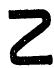
\includegraphics[keepaspectratio]{images/part002_bec1605a.jpg}}

一般说来，即使在波兰空间中，苏斯林子空间的余集也未必是苏斯林的（参看习题 6）；但参看第 6 号定理 2 的推论。

命题 9. 设 X 是可度量化空间，A 是 X 的相对紧苏斯林子空间。则存在一个紧可度量化空间 K 、K 的子集的一个递减序列 \((\mathbf{B}_{n})\) （其中每个子集都是紧集的可数并）以及一个连续映射 \(f: K \to X\) ，使得 \(A = f\left(\bigcap_{n} B_{n}\right)\) 。

必要时以 \(\overline{\mathbf{A}}\) 代替 X ，可设 X 是紧的且 A 在 X 中稠密。由于 A 是苏斯林空间，存在波兰空间 P 与连续映射 \(g: \mathrm{P} \to \mathrm{X}\) 使 \(g(\mathrm{P}) = \mathrm{A}\) 。由第 1 号定理 1 的推论 1 ，可设 P 是递减序列 \((\mathbf{U}_n)\) 的交，其中诸项是方体 \(\mathbf{I}^{\mathbf{N}}\) 的开子集。设 K 为空间 \(\mathbf{I}^{\mathbf{N}} \times \mathbf{X}\) ，它是紧且可度量化的（§ 2，第 4 号，定理 1 的推论 2）。设 \(\mathbf{G} \subset \mathbf{P} \times \mathbf{X}\) 是 \(g\) 的图像，\(\overline{\mathbf{G}}\) 是 G 在 K 中的闭包，而 \(f\) 表示 \(\mathbf{K} = \mathbf{I}^{\mathbf{N}} \times \mathbf{X}\) 到 X 上的投影；则显然有 \(f(\mathbf{G}) = \mathbf{A}\) 。由于 \(g\) 连续，G 在 \(\mathbf{P} \times \mathbf{X}\) 中闭（第 I 章，§ 8，第 1 号，命题 2 的推论 2），且 \(\mathbf{G} = \overline{\mathbf{G}} \cap (\mathbf{P} \times \mathbf{X})\) ；故 \(\mathbf{G} = \bigcap_{n=1}^{n} \mathbf{B}_n\) ，其中

\[
\mathbf {B} _ {n} = \overline {{\mathbf {G}}} \cap (\mathbf {U} _ {n} \times \mathbf {X}).
\]

由于每个 \(U_{n}\) 都是 \(I^{N}\) 中闭集的可数并（§ 2，第 5 号，命题 7），每个 \(B_{n}\) 都是紧集的可数并，证明完毕。

\subsection{波莱尔集}

定义 3. 设 X 是一个集，\(\mathfrak{X}\) 是 X 的子集所成的一个集。\(\mathfrak{X}\) 称为 X 上的一个 \(\sigma\) 代数，如果下列条件满足：

\begin{enumerate}
\def\labelenumi{\alph{enumi})}
\item
  \(\mathfrak{S}\) 中每个集的余集属于 \(\mathfrak{S}\) 。
\item
  \(\mathfrak{X}\) 中集合的每个可数交属于 \(\mathfrak{X}\) 。
\end{enumerate}

若 \(\mathfrak{X}\) 是一个 \(\sigma\) 代数（在 \(\mathbf{X}\) 上），则 \(\mathfrak{X}\) 中集合的每个可数并都属于 \(\mathfrak{X}\) （因为此并的余集是 \(\mathfrak{X}\) 中集合的交）。

X 的所有子集所成的集 \(\mathfrak{P}(\mathbf{X})\) 显然是一个 \(\sigma\) 代数。X 上的 \(\sigma\) 代数的每个交是 X 上的 \(\sigma\) 代数。因此，对 \(\mathfrak{P}(\mathbf{X})\) 的任意子集 F ，存在包含 F 的最小 \(\sigma\) 代数；它称为由 F 生成的 \(\sigma\) 代数。

定义 4. 在拓扑空间 X 中，由 X 的所有闭子集所成的集生成的 \(\sigma\) 代数的元素称为 X 中的波莱尔集。

命题 10. 设 \(f\) 是拓扑空间 \(\mathbf{X}\) 到拓扑空间 \(\mathbf{Y}\) 中的连续映射。则在 \(f\) 之下，\(\mathbf{Y}\) 中每个波莱尔集的原像是 \(\mathbf{X}\) 中的波莱尔集。

设 \(\mathfrak{X}\) 是满足如下条件的诸集 \(\mathbf{A}\) （ \(\mathbf{Y}\) 的子集）所成的集：\(\overline{f}^1 (\mathbf{A})\) 是 \(\mathbf{X}\) 中的波莱尔集。由此立得 \(\mathfrak{X}\) 是一个 \(\sigma\) 代数，它包含 \(\mathbf{Y}\) 的所有闭子集；从而 \(\mathfrak{X}\) 包含 \(\mathbf{Y}\) 中的所有波莱尔集。

命题 11. 在苏斯林空间 X 中，每个波莱尔集都是苏斯林集。

设 \(\mathfrak{X}\) 是由 X 的诸子集 A 中 A 与 CA 都是苏斯林集者所成的集。由第 2 号的命题 8 ，\(\mathfrak{X}\) 是一个 \(\sigma\) 代数。X 的每个闭子集 F 属于 \(\mathfrak{X}\) ，因为 F 与 CF 都是苏斯林集（第 2 号，命题 5）；从而 \(\mathfrak{X}\) 包含 X 的所有波莱尔集（参看第 6 号，定理 2 的推论）。

推论. 设 \(f\) 是苏斯林空间 \(\mathbf{X}\) 到可度量化空间 \(\mathbf{Y}\) 中的连续映射。若 \(\mathbf{B}\) 是 \(\mathbf{X}\) 中的任意波莱尔集，则 \(f(\mathbf{B})\) 是 \(\mathbf{Y}\) 中的苏斯林集。

因为 B 是苏斯林空间，故由定义 2 后的注（第 2 号），\(f(\mathbf{B})\) 也是苏斯林空间。

\pandocbounded{
\includegraphics[keepaspectratio]{images/part002_bde2d1b5.jpg}}

注。1) 即使 X 与 Y 都是波兰空间，一般说来，X 中的波莱尔集在 X 到 Y 中的连续映射下的像未必是 Y 中的波莱尔集（参看习题 6；以及第 7 号，定理 3 的推论）。

\begin{enumerate}
\def\labelenumi{\arabic{enumi})}
\setcounter{enumi}{1}
\tightlist
\item
  设 X 是拓扑空间，Y 是 X 的波莱尔子集。则空间 Y 的波莱尔集恰是 X 的含于 Y 的那些波莱尔集。因为 (i) X 中含于 Y 的波莱尔集构成 Y 上的一个 σ 代数，它包含 Y 中的闭集，从而包含 Y 的所有波莱尔集；(ii) X 的使 A∩Y 是 Y 的波莱尔集的那些子集 A 构成 X 上的一个 σ 代数，它包含 X 的所有闭集，从而包含 X 的所有波莱尔集。
\end{enumerate}

\subsection{零维空间与卢津空间}

定义 5. 拓扑空间称为零维的，如果它是豪斯多夫的，且每个点有一个既开又闭的邻域基本系。

每个零维空间 X 都是全不连通的；因为一点的连通分支含于所有包含该点且既开又闭的集（第 I 章，§ 11，第 5 号），而这些集的交正是 \(\{x\}\) ，若 \(\mathbf{X}\) 是零维的。

反之，局部紧全不连通空间是零维的（第 II 章，§ 4，第 4 号，命题 6）；但存在不是零维的全不连通可度量化空间{[}习题 3 b){]}。

零维空间的每个子空间是零维的，且零维空间的拓扑和与积是零维的。

定义 6. 拓扑空间 X 是卢津空间，如果它可度量化，且存在一个零维波兰空间 P 和 P 到 X 上的连续双射映射。

显然每个卢津空间都是苏斯林空间。

命题 12. 可度量化空间是卢津空间，当且仅当它是一个波兰空间在连续双射映射下的像。

此条件显然必要；我们证明它也充分。若 f 是卢津空间 X 到可度量化空间 Y 上的连续双射，则由定义 6 ，Y 是卢津空间。故只需证明波兰空间是卢津空间。

首先注意，若 X 是卢津空间，则 X 的每个闭（相应地，开）子空间 A 是卢津空间（参看第 7 号，定理 3）；因为若 f 是零维波兰空间 P 到 X 上的连续双射，则 \(\overline{f}^{1}(A)\) 在 P 中闭（相应地，开），因而是 P 的零维波兰子空间（第 1 号，命题 1 与命题 2）。

卢津空间的每个可数积是卢津空间；这由第 1 号的命题 1 及零维空间的每个积是零维的这一事实得出。豪斯多夫拓扑空间中卢津子空间的每个可数交是卢津子空间；这由前面的注及第 1 号的引理 1 得出。此外：

引理 2. 若可度量化空间 X 使得存在 X 的一个由卢津子空间组成的可数分划 \((\mathbf{A}_{n})\) ，则 X 是卢津空间。

对每个 n ，设 \(P_{n}\) 是零维波兰空间，\(f_{n}\) 是 \(P_{n}\) 到 \(A_{n}\) 上的连续双射。若 P 是诸 \(P_{n}\) 的拓扑和，则 P 是波兰的（第 1 号，命题 1）且零维，而映射 \(f: P \to X\) （它与 \(f_{n}\) 在每个 \(P_{n}\) 上（对每个 n ）一致）是 P 到 X 上的连续双射；由此即得结论。

现在证明 R 的区间 \(I = [0, i]\) 是卢津空间。设 J 是由 I 中所有无理数组成的子空间；则 J 是波兰空间（第 1 号，命题 3 的推论）；且 J 是零维的，因为若 x 是 J 的任意点，则 R 中形如 {]}r, s{[} （其中 r 与 s 是有理数且 r \textless{} x \textless{} s ）的区间在 J 上的迹构成 x 在 J 中的既开又闭邻域的基本系（因为 {]}r, s{[} 与 {[}r, s{]} 在 J 上的迹相同）。故 J 是 I 的卢津子空间。而 J 与 I 的每个由单个有理点组成的子空间构成 I 的可数分划，因此由引理 2 ，I 是卢津空间。

设 P 是任意波兰空间。由定理 1 的推论 1 （第 1 号），P 同胚于方体 IN 的一个子空间，后者是 IN 中开集的可数交。由于 I 是卢津空间，证明开头的诸注表明 P 是卢津空间，从而命题 12 的证明完成。

\subsection{筛}

定义 7. 筛是一个序列 \(\mathbf{C} = (\mathbf{C}_n, p_n)_{n \geqslant 0}\) ，使得对每个 \(n\) ，\(\mathbf{C}_n\) 是可数集，而 \(p_n\) 是 \(\mathbf{C}_{n+1}\) 到 \(\mathbf{C}_n\) 上的满射。

对每对整数 \(m, n\) （满足 \(0 \leqslant m \leqslant n\) ），令 \(p_{mn}\) 表示 \(C_m\) 到自身的恒等映射（若 \(m = n\) ），或映射 \(p_m \circ p_{m+1} \circ \cdots \circ p_{n-1}\) （它是 \(C_n\) 到 \(C_m\) 上的满射，若 \(m < n\) ）。显然 \(p_{mq} = p_{mn} \circ p_{ng}\) 对 \(m \leqslant n \leqslant q\) 成立，因此可以考虑 \(L(C)\) ，即族 \((C_n)\) 关于映射族 \((p_{mn})\) 的逆极限（集合论，第 III 章，§ 7）。若每个 \(C_n\) 赋以离散拓扑，则 \(L(C)\) 是拓扑空间的逆极限（第 I 章，§ 4，第 4 号）；作为这样的空间，\(L(C)\) 称为与筛 \(C\) 相伴的拓扑空间。\(L(C)\) 是拓扑积 \(\prod_n C_n\) 的闭子空间，由此立得 \(L(C)\) 是零维波兰空间（第 4 号）。

度量空间 X 的一个筛分由一个筛 \(\mathbf{C} = (\mathbf{C}_{n}, p_{n})\) 以及对每个整数 \(n \geqslant 0\) 的一个映射 \(\varphi_{n}\) 组成，后者把 \(C_{n}\) 映到 X 的直径 \(\leqslant 2^{-n}\) 的非空闭子集所成的集中，且满足：

\begin{enumerate}
\def\labelenumi{\alph{enumi})}
\item
  X 是诸集 \(\varphi_0(c)\) （当 \(c\) 跑遍 \(\mathbf{C}_0\) ）的并；
\item
  对每个 \(n\) 与每个 \(c \in \mathbf{C}_n\) ，\(\varphi_n(c)\) 是诸集 \(\varphi_{n+1}(c')\) （其中 \(c'\) 跑遍 \(\overline{\pmb{p}}_n(c)\) ）的并。
\end{enumerate}

筛分称为严格筛分，如果此外对每个 n ，诸集 \(\varphi_{n}(c)\) （当 c 跑遍 \(C_{n}\) ）两两不相交。

引理 3. 每个可数型度量空间 X 都具有一个筛分。若 X 还是零维的，则 X 具有严格筛分。

首先注意，若 Y 是可数型度量空间，\(\varepsilon\) 是实数 \textgreater0 ，则存在 Y 的由直径 \(\leqslant\varepsilon\) 的集组成的可数覆盖（§2，第 8 号，命题 13）。此外，若 Y 是零维的，则存在这样的、由既开又闭的集组成的覆盖 \((\mathbf{V}_{n})\) ；若 \(W_{n}\) 是 \(V_{n}\) 与 \(\bigcap_{k<n}(\mathbf{Y}-\mathbf{V}_{k})\) 的交，则可见诸 \(W_{n}\) 是闭的、直径 \(\leqslant\varepsilon\) 、两两不相交且覆盖 X。无论如何，覆盖中非空集的闭包构成 Y 的一个可数覆盖，其元素是直径 \(\leqslant\varepsilon\) 的非空闭集。

设 X 是可数型度量空间。设 \(C_{0}\) 是 X 的一个由直径 \(\leqslant I\) 的非空闭集组成的可数覆盖的指标集（若 X 是零维的，这些集两两不相交）；\(\varphi_{0}\) 是使每个指标 \(c \in C_{0}\) 对应于覆盖中相应集的映射。设我们已定义了诸 \(C_{i}\) 、诸 \(\varphi_{i}\) 与满射映射 \(p_{i}: C_{i+1} \to C_{i}\) （对 \(i \leqslant n\) ），使得对这些指标条件 b) 满足。若 \(c \in C_{n}\) ，则空间 \(\varphi_{n}(c)\) 有一个由直径 \(\leqslant I/2^{n+1}\) 的非空闭集组成的可数覆盖（若 X {[}从而 \(\varphi_{n}(c)\) {]}是零维的，这些集两两不相交）；若 \(\mathrm{I}(c)\) 表示此覆盖的指标集，我们取 \(c_{n+1}\) 为诸集 \(\mathrm{I}(c)\) （当 c 跑遍 \(C_{n}\) ）之和；对每个 \(c' \in C_{n+1}\) ，令 \(p_{n}(c')\) 表示元素 \(c \in C_{n}\) 中满足 \(c' \in \mathrm{I}(c)\) 者，并令 \(\varphi_{n+1}(c')\) 表示指标为 \(c'\) 的集（在所考虑的 \(\varphi_{n}(c)\) 的覆盖中）。显然我们这样归纳地定义了 X 的一个筛分，且若 X 是零维的，此筛分是严格的；由此得引理 3 。

现在设 X 是可数型完备度量空间，考虑 X 的由一个筛 C 与诸映射 \(\varphi_{n}\) 给出的一个筛分。若 \(\gamma = (c_{n})\) 是与 C 相伴的空间 \(\mathrm{L}(\mathrm{C})\) 的一点，则序列 \((\varphi_{n}(c_{n}))\) 是 X 中闭集的递减序列，其直径趋于 0 ；因此这序列的集的交由单独一点组成，我们记之为 \(f(\gamma)\) 。这样我们就定义了一个映射 \(f: \mathrm{L}(\mathrm{C}) \to \mathrm{X}\) 。若 \(\gamma, \gamma'\) 是 \(\mathrm{L}(\mathrm{C})\) 的两点，它们对 \(i \leqslant n\) 有相同的第 i 坐标，则显然 \(f(\gamma)\) 与 \(f(\gamma')\) 之间的距离 \(\leqslant 1/2^{n}\) ，从而 f 是连续的（由 \(\mathrm{L}(\mathrm{C})\) 的拓扑的定义）。对每个 \(x \in X\) ，由筛分的定义可用对 n 的归纳定义一个序列 \(\gamma = (c_{n})\) ，使得 \(x \in \varphi_{n}(c_{n})\) 对每个 \(n \geqslant 0\) 成立，且 \(c_{n} = p_{n}(c_{n+1})\) ；因此 \(x = f(\gamma)\) ，故 f 是满射。此外，若筛分是严格的，则序列 \(\gamma = (c_{n})\) （它满足 \(x = f(\gamma)\) ）是唯一的，故在此情形 f 是双射。f 称为所考虑筛分诱导的映射。

命题 13. 若 X 是任意卢津（相应地，苏斯林）空间，则存在一个筛 C 与 L(C) 到 X 上的连续双射（相应地，满射）。

参照卢津空间的定义（第 4 号，定义 6）{[}相应地，苏斯林空间的定义（第 2 号，定义 2）{]}，我们归结到如下情形：

X 是零维波兰空间（相应地，波兰空间），而前面的论证随即证明此结果。

\subsection{苏斯林集的分离}

定理 2. 设 X 是可度量化空间。若给定 X 的两两不相交的苏斯林子空间的一个序列 \((\mathbf{X}_{n})\) ，则存在 X 中两两不相交的波莱尔集的一个序列 \((\mathbf{B}_{n})\) ，使得对每个 n 有 \(X_{n} \subset B_{n}\) 。

证明基于两个引理：

引理 4. 设 \((\mathbf{A}_n), (\mathbf{A}_m')\) 是拓扑空间 \(\mathbf{X}\) 的子集的两个序列。假设对每对 \((\mathbf{A}_n, \mathbf{A}_m')\) 有一个波莱尔集 \(\mathbf{B}_{nm}\) （ \(\mathbf{X}\) 中的），使得 \(\mathbf{B}_{nm} \supset \mathbf{A}_n\) 且 \(\mathbf{B}_{nm} \cap \mathbf{A}_m' = \emptyset\) 。则存在一个波莱尔集 \(\mathbf{B}\) （ \(\mathbf{X}\) 中的），它包含 \(\bigcup_{n} \mathbf{A}_n\) 且不交 \(\bigcup_{m} \mathbf{A}_m'\) 。

因为波莱尔集 \(\mathbf{B} = \bigcup_{n}\left(\bigcap_{m}\mathrm{B}_{nm}\right)\) 满足这些条件。

引理 5. 设 X 是豪斯多夫空间，A 、A' 是 X 的两个不相交的苏斯林子空间。则存在 X 的一个波莱尔集 B ，使得 B ⊃ A 且 B ∩ A' = ∅。

由第 5 号的命题 13 ，存在两个筛 \(\mathbf{C}\) 、\(\mathbf{C}'\) 与连续映射 \(f\) （ \(\mathbf{L}(\mathbf{C})\) 到 \(\mathbf{A}\) 上的）、\(f'\) （ \(\mathbf{L}(\mathbf{C}')\) 到 \(\mathbf{A}'\) 上的），它们用第 5 号中描述的方法构造。对每个 \(n \geqslant 0\) 与每个 \(c \in \mathbf{C}_n\) ，令 \(q_n(c)\) 表示 \(\mathbf{L}(\mathbf{C})\) 中由一切序列 \((c_k)_{k \geqslant 0}\) （满足 \(c_n = c\) 者）所成的子空间；\(q_n(c)\) 是 \(\mathbf{L}(\mathbf{C})\) 的闭子空间。对每个 \(\gamma = (c_n) \in \mathbf{L}(\mathbf{C})\) ，闭集序列 \(q_n(c_n)\) 是递减的，且构成以 \(\gamma\) 为极限的滤基。此外，对每个 \(c \in \mathbf{C}_n\) ，诸集 \(q_{n+1}(d)\) （其中 \(d\) 跑遍集 \(\overline{p_n}(c)\) ，此集在 \(\mathbf{C}_{n+1}\) 中）构成 \(q_n(c)\) 的一个分划。对筛 \(c'\) 作类似的记号定义。

我们将用反证法，假设每个包含 A 的波莱尔集都与 \(A'\) 相交。首先，由引理 4 与筛分的定义，存在 \(c_{0} \in C_{0}\) 与 \(c_{0}' \in C_{0}'\) ，使得每个包含 \(f(q_{0}(c_{0}))\) 的波莱尔集都与 \(f'(q_{0}'(c_{0}'))\) 相交。然后我们可以对 n 用归纳法定义

\[
\gamma = (c _ {n}) \in \mathrm{L} (\mathrm{C}) \quad \text { and } \quad \gamma^ {\prime} = (c _ {n} ^ {\prime}) \in \mathrm{L} (\mathrm{C} ^ {\prime})
\]

如下：设 \(c_i\) 与 \(c_i'\) 已对 \(i < n\) 定义，使得对每个指标 \(i < n\) ，每个包含 \(f(q_i(c_i))\) 的波莱尔集都与 \(f'(q_i'(c_i'))\) 相交；把引理 4 与筛分的定义应用于集 \(f(q_{n-1}(c_{n-1}))\) 与 \(f'(q_{n-1}'(c_{n-1}'))\) ，即见存在 \(c_n \in \mathbf{C}_n\) 与 \(c_n' \in \mathbf{C}_n'\) ，使得 \(p_{n-1}(c_n) = c_{n-1}\) 且 \(p_{n-1}(c_n') = c_{n-1}'\) 。

并使得每个包含 \(f(q_n(c_n))\) 的波莱尔集都与 \(f'(q_n'(c_n'))\) 相交。而序列 \(f(q_n(c_n))\) 收敛于一点 \(a = f(\gamma) \in \mathbf{A}\) ，序列 \(f'(q_n'(c_n'))\) 收敛于一点 \(a' = f'(\gamma') \in \mathbf{A}'\) 。由于 \(\mathbf{A} \cap \mathbf{A}' = \emptyset\) 且 \(\mathbf{X}\) 是豪斯多夫的，存在一个闭邻域 \(\mathbf{V}\) （ \(a\) 的），它不含 \(a'\) ，从而对充分大的 \(n\) ，\(\mathbf{V}\) 包含 \(f(q_n(c_n))\) 且不交 \(f'(q_n'(c_n'))\) 。这是矛盾，因为 \(\mathbf{V}\) 是波莱尔集。

为证定理 2 ，令 \(\mathbf{Y}_n\) 表示诸集 \(\mathbf{X}_i\) （满足 \(i \neq n\) 者）的并；则 \(\mathbf{Y}_n\) 是 \(\mathbf{X}\) 的苏斯林子空间（第 2 号，命题 8）。由引理 5 ，对每个指标 \(n\) 存在波莱尔集 \(\mathbf{B}_n'\) ，它包含 \(\mathbf{X}_n\) 且不交 \(\mathbf{Y}_n\) 。令 \(\mathbf{B}_n\) 为 \(\mathbf{B}_n'\) 与 \(\bigcap_{i < n} (\mathbf{X} - \mathbf{B}_i')\) 的交。则诸 \(\mathbf{B}_n\) 是波莱尔集，两两不相交，且 \(\mathbf{B}_n \supset \mathbf{X}_n\) 对每个 \(n\) 成立。

推论. 若可度量化空间的一个可数分划由苏斯林集组成，则这些集是波莱尔集。特别地，可度量化空间中余集为苏斯林集的每个苏斯林集是波莱尔集。

\subsection{卢津空间与波莱尔集}

定理 3. 设 X 是卢津空间。则 X 的子空间是卢津空间，当且仅当它是波莱尔集。

此定理是下述两个引理的推论：

引理 6. 在卢津空间 X 中，每个波莱尔集都是 X 的卢津子空间。

设 \(\mathfrak{X}\) 是由 X 的诸子集 A 中 A 与 \(\complement A\) 都是 X 的卢津子空间者所成的集。由于 X 中每个闭集与每个开集都是 X 的卢津子空间（第 4 号），\(\mathfrak{X}\) 包含 X 的所有闭子集，因此只要证明 \(\mathfrak{X}\) 是 X 上的一个 \(\sigma\) 代数，引理即得证。为此只需证明：若 \((A_n)\) 是 \(\mathfrak{X}\) 中集合的一个序列，则 \(\bigcap_{n} A_n\) 与 \(\bigcup_{n} A_n\) 都是 X 的卢津子空间。我们在第 4 号中已看到，卢津子空间的每个可数交是卢津子空间。另一方面，若 \(B_n\) 是 \(A_n\) 与 \(\bigcap_{i < n} \complement A_i\) 的交，则由假设与前面的注，\(B_n\) 是卢津子空间；且由于 \(\bigcup_{n} A_n = \bigcup_{n} B_n\) ，由第 4 号的引理 2 ，子空间 \(\bigcup_{n} A_n\) 是卢津子空间。

引理 7. 可度量化空间 X 的每个卢津子空间 A 都是 X 中的波莱尔集。

由第 5 号的命题 13 ，存在一个筛 C 与一个连续双射 \(f\) （ \(\mathbf{L}(\mathbf{C})\) 到 A 上的）。用第 6 号引理 5 的记号，对每个整数 \(n\) 与每个 \(c \in \mathbf{C}_n\) ，令 \(g_n(c)\) 表示 X 的子空间 \(f(q_n(c))\) ；它是卢津子空间，因而是 X 的苏斯林子空间。当 \(c\) 跑遍 \(\mathbf{C}_n\) 时，诸集 \(g_n(c)\) 两两不相交，因为 \(f\) 是双射；故由第 6 号的定理 2 ，存在 X 中波莱尔集的一个族 \(c \to g_n'(c) (c \in \mathbf{C}_n)\) ，两两不相交，且使 \(g_n'(c) \supset g_n(c)\) 对一切 \(c \in \mathbf{C}_n\) 成立。必要时以 \(g_n'(c)\) 与闭包 \(\overline{g_n(c)}\) （即 \(g_n(c)\) 在 X 中的闭包）的交代替之，可设 \(g_n'(c) \subset \overline{g_n(c)}\) 。令 \(c_{n-1}, c_{n-2}, \ldots, c_0\) 表示 \(c\) 在 \(\mathbf{C}_{n-1}, \mathbf{C}_{n-2}, \ldots, \mathbf{C}_0\) 中的像，所用满射为

\[
p _ {n - 1, n} = p _ {n - 1}, p _ {n - 2, n} = p _ {n - 2} \circ p _ {n - 1}, \dots , p _ {0 n} = p _ {0} \circ p _ {1} \circ \dots \circ p _ {n - 1}
\]

（分别为）；并令 \(h_n(c)\) 表示下列诸集

\[
g _ {n} ^ {\prime} (c), g _ {n - 1} ^ {\prime} \left(c _ {n - 1}\right), \dots , g _ {o} ^ {\prime} \left(c _ {0}\right).
\]

的交。由于 \(q_{i}(c_{i}) \supset q_{n}(c)\) 对 \(0 \leqslant i \leqslant n - 1\) 成立，\(h_{n}(c)\) 包含 \(g_{n}(c)\) ；同样显然 \(h_{n}(c)\) 是波莱尔集且含于 \(g_{n}(c)\) ，且当 \(c\) 跑遍 \(\mathbf{C}_{n}\) 时诸 \(h_{n}(c)\) 两两不相交；最后，由构造，对每个 \(c' \in \mathbf{C}_{n+1}\) 有 \(h_{n+1}(c') \subset h_n(p_n(c'))\) 。令 \(\mathbf{B}_n\) 为诸集 \(h_n(c)\) （当 \(c\) 跑遍 \(\mathbf{C}_n\) ）的并；\(\mathbf{B}_n\) 是波莱尔集，且 \(\mathbf{B}_{n+1} \subset \mathbf{B}_n\) ；又 \(\mathbf{B}_n\) 包含诸集 \(g_n(c) (c \in \mathbf{C}_n)\) 的并，即 A 。令 B 为递减集序列 \(\mathbf{B}_n\) 的交；B 是波莱尔集且包含 A 。我们将证明 B = A ，这样就完成了证明。

设 \(x\) 是 \(\mathbf{B}\) 的一点。则对每个整数 \(n\) ，存在唯一的 \(c \in \mathbf{C}_n\) 使 \(x \in h_n(c)\) ；我们把此 \(c\) 记作 \(c_n(x)\) 。序列 \((c_n(x))_{n \geqslant 0}\) 属于 \(\mathbf{L}(\mathbf{C})\) 。递减序列 \((g_n(c_n(x)))\) 依定义收敛于一点 \(a \in \mathbf{A}\) ；这些集的闭包序列也收敛于 \(a\) （在 \(\mathbf{X}\) 中），故序列 \((h_n(c_n(x)))\) 更加如此。而 \(x\) 属于所有集 \(h_n(c_n(x))\) ，因此 \(x = a \in \mathbf{A}\) 。引理 7 由此得证，定理 3 亦随之得证。

推论. 若 \(f\) 是卢津空间（特别地，波兰空间）\(\mathbf{X}\) 到可度量化空间 \(\mathbf{Y}\) 中的连续单射映射，则 \(f(\mathbf{X})\) 是 \(\mathbf{Y}\) 中的波莱尔集。

\subsection{波莱尔截面}

定理 4. 设 X 是波兰空间，R 是 X 上的一个等价关系，使得模 R 的等价类在 X 中闭，且 X 中每个闭集（关于 R ）的饱和集是波莱尔集。则存在 X 中的一个波莱尔集，它与每个等价类恰交于一点。

取 X 上与它的拓扑相容且使 X 完备的一个度量。由第 5 号的引理 3 ，存在 X 的一个筛分，由一个筛 \(\mathbf{C} = (\mathbf{C}_{n}, p_{n})\) 与一个映射序列 \((\varphi_{n})\) 定义。对每个 \(c \in C_{n}\) ，令 \(g_{n}(c)\) 为闭集 \(\varphi_{n}(c)\) 关于 R 的饱和集；由假设，\(g_{n}(c)\) 是 X 中的波莱尔集。

由于每个集 \(\mathbf{C}_n\) 可数，我们可以把每个 \(\mathbf{C}_n\) 线性排序，使得小于一个给定元素的元素之集有限。对每个 \(c \in \mathbf{C}_n\) ，我们定义一个集 \(h_n(c)\) ，用对 \(n\) 的归纳，如下。首先，对 \(c \in \mathbf{C}_0\) ，\(h_0(c)\) 是 \(\varphi_0(c)\) 与诸集 \(\mathbf{X} - g_0(c')\) （其中 \(c' \in \mathbf{C}_0\) 且 \(c' < c\) ）的交。对 \(c \in \mathbf{C}_{n+1}\) ，\(h_{n+1}(c)\) 是 \(\varphi_{n+1}(c)\) 、\(h_n(\mathbf{P}_n(c))\) 与诸集 \(\mathbf{X} - g_{n+1}(c')\) （对 \(c' \in \mathbf{C}_{n+1}\) ，\(p_n(c') = p_n(c)\) 且 \(c' < c\) ）的交。诸 \(h_n(c)\) 显然是波莱尔集。

我们将证明下述断言：对每个整数 \(n \geqslant 0\) 与每个等价类 \(\mathbf{H} \mod \mathbb{R}\) ，存在唯一的元素 \(c \in \mathbf{C}_n\) 使 \(h_n(c)\) 与 \(\mathbf{H}\) 相交，且我们有

\[
h (c _ {n}) \cap \mathrm{H} = \varphi_ {n} (c) \cap \mathrm{H},
\]

它因而是闭集。对 \(n = 0\) ，考虑最小的元素 \(c \in \mathbf{C}_0\) （使 \(\varphi_0(c)\) 与 \(\mathbf{H}\) 相交者）；则 \(\varphi_0(c) \cap \mathbf{H}\) 不交任何集 \(g_0(c')\) （对满足 \(c' \in \mathbf{C}_0\) 且 \(c' < c\) 的 c' ）；故它含于 \(h_0(c) \cap \mathbf{H}\) ，从而等于此集；此外，我们有 \(\mathbf{H} \subset g_0(c)\) ，因此 \(h_0(c') \cap \mathbf{H}\) 为空（对 \(c' \in \mathbf{C}_0\) 且 \(c' > c\) ）；这样断言对 \(n = 0\) 得证。我们对 \(n\) 继续用归纳法：若存在 \(c \in \mathbf{C}_{n+1}\) 使 \(h_{n+1}(c)\) 与 \(\mathbf{H}\) 相交，则由关系 \(h_{n+1}(c) \subset h_n(p_n(c))\) 与归纳假设，\(p_n(c)\) 是唯一的元素 \(d \in \mathbf{C}_n\) （使 \(h_n(d)\) 与 \(\mathbf{H}\) 相交者）。注意 \(h_n(d)\) 含于 \(\varphi_n(d)\) ，由筛分的定义，它含于诸集 \(\varphi_n(c)\) （对 \(c \in p_n(d)\) ）的并；因此存在最小元素 \(c \in p_n(d)\) 使 \(\varphi_{n+1}(c)\) 与 \(\mathbf{H}\) 相交。因此我们有

\[
\varphi_ {n + 1} (c) \cap \mathrm{H} \subset \varphi_ {n} (d) \cap \mathrm{H} = h _ {n} (d) \cap \mathrm{H}
\]

（依归纳假设）。从而

\[
\varphi_ {n + 1} (c) \cap \mathrm{H} \subset \varphi_ {n + 1} (c) \cap h _ {n} (d),
\]

且由于依定义 \(\varphi_{n+1}(c) \cap \mathbf{H}\) 不交任何集 \(g_{n+1}(c')\) （对满足 \(c' \in p_n(d)\) 且 \(c' < c\) 的 c' ），由 \(h_{n+1}(c)\) 的定义即得 \(\varphi_{n+1}(c) \cap \mathbf{H} = h_{n+1}(c) \cap \mathbf{H}\) 。此外，我们有 \(\mathbf{H} \subset g_{n+1}(c)\) ，因此若 \(c' \in p_n(d)\) 满足 \(c' > c\) ，则 \(h_{n+1}(c') \cap \mathbf{H}\) 为空。这样断言对一切 \(n\) 得证。

对每个整数 \(n\) ，令 \(\mathbf{S}_n\) 为诸集 \(h_n(c)\) （其中 \(c\) 跑遍 \(\mathbf{C}_n\) ）的并。集 \(\mathbf{S}_n\) 是波莱尔集，且我们有 \(\mathbf{S}_{n+1} \subset \mathbf{S}_n\) 。

令 S 为诸集 \(S_{n}\) 的交，它也是 X 中的波莱尔集；我们将证明 S 与每个等价类 H 模 R 恰交于一点。对每个 n ，令 \(c_{n}(H)\) 为唯一的元素 \(c \in C_{n}\) （使 \(h_{n}(c)\) 与 H 相交者）；则 \(\mathbf{S}_{n} \cap \mathbf{H} = \varphi_{n}(c_{n}(\mathbf{H})) \cap \mathbf{H}\) ，而 \(S \cap H\) 是诸集 \(\varphi_{n}(c_{n}(\mathbf{H})) \cap \mathbf{H}\) 的交。由于序列 \((c_{n}(\mathbf{H}))\) 属于 L(C)，闭集的递减序列 \(\varphi_{n}(c_{n}(\mathbf{H}))\) —— 其直径趋于 0 —— 收敛于一点 \(x \in X\) ，因为 X 完备。诸闭集 \(\varphi_{n}(c_{n}(\mathbf{H})) \cap \mathbf{H}\) 的交因此由单独一点 x 组成，定理 4 的证明完成。

注. 特别地，闭等价关系 R 满足定理 4 的假设。当 X 是紧可度量化空间时，定理 4 因此适用于任意豪斯多夫等价关系 R ，因为紧空间上的豪斯多夫等价关系是闭的（第 I 章，§ 10，第 4 号，命题 8）。

\subsection{苏斯林集的可容性}

定义 8. 设 X 是豪斯多夫拓扑空间。X 上的一个容度是 X 的所有子集所成的集 \(\mathfrak{P}(\mathbf{X})\) 到扩充实直线 \(\overline{\mathbf{R}}\) 中的一个映射 f ，满足下列条件：

\((\mathbf{CA}_{\mathbf{I}})\) 若 \(\mathbf{A} \subset \mathbf{B}\) ，则 \(f(\mathbf{A}) \leqslant f(\mathbf{B})\) 。

\((\mathbf{CA}_{\mathbf{II}})\) 若 \((\mathbf{A}_n)\) 是 \(\mathbf{X}\) 的子集的任意递增序列，则

\[
f \left(\bigcup_ {n} \mathrm{A} _ {n}\right) = \sup _ {n} f (\mathrm{A} _ {n}).
\]

\((\mathbf{CA}_{\mathbf{III}})\) 若 \((\mathbf{K}_n)\) 是 \(\mathbf{X}\) 的紧子集的任意递减序列，则

\[
f \left(\bigcap_ {n} \mathrm{K} _ {n}\right) = \inf _ {n} f (\mathrm{K} _ {n}).
\]

例。* 设 \(\mu\) 是局部紧空间 X 上的一个正测度；则对应的外测度 \(\mu^{*}\) 是 X 上的一个容度。可以证明，在欧氏空间 \(\mathbf{R}^{n}\) （ \(n \geqslant 3\) ）中，“牛顿外容度”是定义 8 意义下的容度。*

定义 9. 设 \(f\) 是 \(\mathbf{X}\) 上的一个容度；子集 \(\mathbf{A}\) （ \(\mathbf{X}\) 的）称为可容的（关于 \(f\) ），如果 \(f(\mathbf{A}) = \sup_k f(\mathbf{K})\) ，其中 \(\mathbf{K}\) 跑遍 \(\mathbf{A}\) 的紧子集所成的集。

* 例如，若 \(f\) 是一个外测度 \(\mu^{*}\) ，则每个开集都是可容的；满足 \(\mu^{*}(A) < +\infty\) 的可容集 A 恰是 \(\mu\) 可积集。*

命题 14. 设 K 是紧空间，f 是 K 上的一个容度。若 A 是 K 的子集的递减序列 \((\mathbf{A}_{n})\) 的交，其中每个子集都是闭集的可数并，则 A 是可容的。

只需证明，对每个 \(a < f(A)\) ，存在闭集 \(\mathbf{C} \subset \mathbf{A}\) 使 \(f(\mathbf{C}) \geqslant a\) 。首先证明存在闭集的一个序列 \((\mathbf{B}_n)_{n \geqslant 1}\) ，使得 \(\mathbf{B}_n \subset \mathbf{A}_n\) ，且使得序列 \((\mathbf{C}_n)\) 若由条件 \(\mathbf{C}_0 = \mathbf{A}\) 、\(\mathbf{C}_n = \mathbf{C}_{n-1} \cap \mathbf{B}_n\) （对 \(n \geqslant 1\) ）归纳地定义，则 \(f(\mathbf{C}_n) > a\) 对每个 \(n \geqslant 0\) 成立。设诸 \(\mathbf{B}_i\) 已对 \(i < n\) 定义；由假设我们有 \(\mathbf{C}_{n-1} \subset \mathbf{A} \subset \mathbf{A}_n\) 与 \(f(\mathbf{C}_{n-1}) > a\) ；由于 \(\mathbf{A}_n\) 是闭集的递增序列 \(\mathbf{D}_j\) 的并，由 \((\mathbf{CA}_{\mathbf{II}})\) 得

\[
f \left(\mathrm{C} _ {n - 1}\right) = \sup _ {j} f \left(\mathrm{C} _ {n - 1} \cap \mathrm{D} _ {j}\right).
\]

因此有一个指标 \(j\) 使 \(f(\mathbf{C}_{n-1} \cap \mathbf{D}_j) > a\) ，而我们可以取 \(\mathbf{B}_n = \mathbf{D}_j\) 。

现在令 \(\mathbf{C} = \bigcap_{n}\mathbf{C}_{n}\) 。由于 \(\mathbf{A} = \bigcap_{n}\mathbf{A}_{n}\) 且 \(\mathbf{B}_n\subset \mathbf{A}_n\) ，我们有

\[
\mathrm{C} = \bigcap_ {n} \mathrm{B} _ {n};
\]

因此集 C 是紧的且含于 A 。

令 \(B_n' = B_1 \cap B_2 \cap \cdots \cap B_n\) ；\((B_n')\) 是 K 的紧子集的递减序列；由于 \(C_n \subset C_i \subset B_i\) 对 i \textless{} n 成立，我们也有 \(C_n \subset B_n'\) 。由 \((CA_{III})\) ，\(f(C) = \inf_{n} f(B_n')\) ，且由于 \(C \subset C_n \subset B_n'\) 我们也有 \(f(C) = \inf_{n} f(C_n) \geqslant a\) 。这就完成了证明。

定理 5. 设 X 是可度量化空间，Y 是 X 的相对紧苏斯林子空间。则 Y 关于 X 上的每个容度 f 都是可容的。

我们已看到（第 2 号，命题 9），存在一个紧空间 K 、K 的子集的递减序列 \((\mathbf{A}_{n})\) （其中每个子集都是紧集的可数并）与一个连续映射 \(\varphi: K \to X\) ，使得 \(Y = \varphi\left(\bigcap_{n} A_{n}\right)\) 。由命题 14 ，\(\bigcap_{n} A_{n}\) 关于 K 上的每个容度都是可容的。因此定理 5 是下述命题的推论：

命题 15. 设 \(\varphi\) 是豪斯多夫空间 K 到豪斯多夫空间 X 中的连续映射，\(f\) 是 X 上的一个容度。若对 K 的每个子集 A 令 \(g(A) = f(\varphi(A))\) ，则 \(g\) 是 K 上的一个容度；此外，若 A 关于 \(g\) 是可容的，则 \(\varphi(A)\) 关于 \(f\) 是可容的。

显然 \(g\) 满足公理 \((\mathbf{CA}_{\mathbf{I}})\) 与 \((\mathbf{CA}_{\mathbf{II}})\) 。另一方面，设 \((\mathbf{C}_n)\) 是 \(\mathbf{K}\) 的紧子集的递减序列，并令 \(\mathbf{C} = \bigcap_{n} \mathbf{C}_n\) ；诸集 \(\varphi(\mathbf{C})\) 是紧的，它们的交是 \(\varphi(\mathbf{C})\) ；因为此交当然包含 \(\varphi(\mathbf{C})\) ，且若 \(x \in \varphi(\mathbf{C}_n)\) 对一切 \(n\) 成立，则诸集 \(\overline{\varphi}^1(x) \cap \mathbf{C}_n\) 构成 \(\mathbf{K}\) 的非空紧子集的递减序列，因此它们的交非空。于是我们有 \(f(\varphi(\mathbf{C})) = \inf_{n} f(\varphi(\mathbf{C}_n))\) ，即 \(g(\mathbf{C}) = \inf_{n} g(\mathbf{C}_n)\) ；这样 \(g\) 满足公理 \((\mathbf{CA}_{\mathbf{III}})\) ，因而是 \(\mathbf{K}\) 上的一个容度。

现在设 A 是 K 的关于 g 可容的子集；若 \(a < f(\varphi(A)) = g(A)\) ，则存在紧集 \(C \subset A\) 使 \(g(C) \geqslant a\) ；这样 \(\varphi(C)\) 是含于 \(\varphi(A)\) 的紧集，且 \(f(\varphi(C)) \geqslant a\) 。这表明 \(\varphi(A)\) 关于 f 是可容的，并完成了命题 15 从而定理 5 的证明。

注. * 若 \(\mu\) 是局部紧可度量化空间 X 上的一个正测度，则 X 的每个苏斯林子集 A 都是 \(\mu\) 可测的。因为若 K 是 X 的任意紧子集，则 K∩A 是相对紧苏斯林集，从而关于 \(\mu^{*}\) 是可容的，因而是 \(\mu\) 可积的。注意苏斯林集在 X 中的余集虽然一般不是苏斯林集，却是 \(\mu\) 可测的 *。

\appendix
\setcounter{chapter}{9}
\renewcommand{\thechapter}{\Roman{chapter}}
\setcounter{subsection}{0}
\renewcommand{\thesubsection}{\arabic{subsection}}

\section*{附录：赋范代数中的无穷乘积}
\phantomsection
\addcontentsline{toc}{section}{附录：赋范代数中的无穷乘积}

\subsection{赋范代数中的可乘序列}

设 A 是非离散赋值域 K 上的一个赋范代数（第 IX 章，§ 3，第 7 号，定义 9）；我们用 \(||x||\) 表示元素 \(x \in A\) 的范数，并设此范数满足不等式 \(||xy|| \leqslant ||x|| \cdot ||y||\) ；又设 A 有单位元 \(e\) 。设 \((x_n)_{n \in \mathbb{N}}\) 是 A 的点的一个无穷序列。N 的每个有限子集 J （以 N 的序线性排序）定义 A 的点的一个序列 \((x_n)_{n \in J}\) ，而我们定义积

\[
p _ {J} = \prod_ {n \in J} x _ {n}
\]

为此序列的积；此积称为序列 \((\pmb{x}_n)_{n\in \mathbb{N}}\) 的对应于有限子集 \(J\) （ \(\mathbb{N}\) 的）的有限部分积（回忆若 \(J = \emptyset\) ，我们令 \(\prod_{n\in \emptyset}x_n = e\) ）。

定义 1. 序列 \((\pmb{x}_n)_{n\in \mathbb{N}}\) 称为在赋范代数 \(\mathbf{A}\) 中可乘的，如果映射 \(\mathbf{J}\to \pmb{p}_{\mathbf{J}}\) 关于有限子集所成的集 \(\mathfrak{F}(\mathbf{N})\) （ \(\mathbf{N}\) 的）的截口滤有极限，此集以关系 \(c\) 排序；此极限称为序列 \((\pmb{x}_n)_{n\in \mathbb{N}}\) 的积，记作 \(\prod_{n\in \mathbb{N}}\pmb{x}_n\) （或简作 \(\prod_{n}\pmb{x}_n\) ）；诸 \(\pmb{x}_n\) 称为此积的因子。

定义 1 等价于下述：序列 \((\pmb{x}_n)\) 可乘且其积为 \(\pmb{p}\) ，如果对每个 \(\varepsilon > 0\) 存在有限子集 \(J_0\) （ \(\mathbf{N}\) 的），使得对每个有限子集 \(J \supset J_0\) （ \(\mathbf{N}\) 的），有 \(||\pmb{p}_{\mathrm{J}} - \pmb{p}|| \leqslant \varepsilon\) 。

注。1) 当 A 是交换代数时，定义 1 与第 III 章，§ 5，第 1 号，注 3 中所给的相同；但当 A 不交换时，指标集 N 的序结构本质上涉及定义 1 。若 \(\sigma\) 是 N 的任意置换，一般不能断言序列 \((\pmb{x}_{\sigma(n)})\) 在序列 \((x_{n})\) 可乘时可乘；且若两个序列都可乘，它们的积一般不同。

\begin{enumerate}
\def\labelenumi{\arabic{enumi})}
\setcounter{enumi}{1}
\tightlist
\item
  定义 1 可以直接推广到族 \((\pmb{x}_n)_{n\in I}\) 的情形，其指标集 I 是 \(\mathbf{Z}\) 的子集（以 \(\mathbf{Z}\) 的序所诱导的序线性排序）。我们将下述结果向此情形的推广留给读者（参看习题 1 与习题 2）。
\end{enumerate}

\subsection{可乘性判别法}

以下我们恒设赋范代数 A 是完备的。

定理 1. 设 \((\pmb{x}_n)_{n\in \mathbb{N}}\) 是完备赋范代数 A 中的点的一个序列。a) 若 \((\pmb{x}_n)\) 可乘且其积是 A 的一个单位，则对每个 \(\varepsilon >0\) 存在 N 的有限子集 \(\mathbf{J}_0\) ，使得对 N 的每个不交 \(\mathbf{J}_0\) 的有限子集 L ，有 \(||e - p_{\mathrm{L}}||\leqslant \varepsilon\) 。

\begin{enumerate}
\def\labelenumi{\alph{enumi})}
\setcounter{enumi}{1}
\item
  反之，若序列 \((\pmb{x}_n)\) 满足此条件，则它可乘。此外，若每个 \(\pmb{x}_n\) 是单位，则 \(\prod_{n\in \mathbb{N}}\pmb{x}_n\) 是单位。
\end{enumerate}

a) 设 \(\pmb{p}\) 是可乘序列 \((\pmb{x}_n)\) 的积，且设 \(\pmb{p}\) 是 A 中的单位；则（第 IX 章，§ 3，第 7 号，命题 13）存在 \(\alpha > 0\) 与 \(a > 0\) ，使得对一切满足如下条件的 \(y \in A\) ：

\[
\left| \left| \boldsymbol {y} - \boldsymbol {p} \right| \right| \leqslant \alpha ,
\]

y 是单位且 \(\|y^{-1}\|\leqslant a\) 。由假设，对每个 \(\varepsilon\) （满足 \(o<\varepsilon<\alpha\) ），存在 N 的有限子集 \(H_{0}\) ，使得对 N 的每个包含 \(H_{0}\) 的有限子集 H ，有 \(\|p_{H}-p\|\leqslant\varepsilon\) 。设 \(J_{0}=[0,m]\) 是包含 \(H_{0}\) 的 N 的一个区间；对 N 的每个不交 \(J_{0}\) 的有限子集 L ，属于 L 的整数都大于属于 \(H_{0}\) 的整数；因此，若 \(H=H_{0}\cup L\) ，我们有 \(p_{H}=p_{H_{0}}p_{L}\) 。现在，由于 \(\|p_{H_{0}}-p\|\leqslant\varepsilon\leqslant\alpha\) ，\(p_{H_{0}}\) 是单位，且

\[
\left| \left| e - p _ {\mathrm{H} _ {0}} ^ {- 1} p \right| \right| \leqslant \varepsilon \left| \left| p _ {\mathrm{H} _ {0}} ^ {- 1} p \right| \right| \leqslant a \varepsilon ;
\]

由于 \(||p_{\mathrm{H_0}}p_{\mathrm{L}} - p|| \leqslant \varepsilon\) ，我们推出

\[
\left| \left| p _ {\mathrm{L}} - p _ {\mathrm{H} _ {0}} ^ {- 1} p \right| \right| \leqslant \varepsilon \left| \left| p _ {\mathrm{H} _ {0}} ^ {- 1} \right| \right| \leqslant a \varepsilon ,
\]

而最终 \(||e - p_{\mathrm{L}}|| \leqslant 2a\varepsilon\) 。

\begin{enumerate}
\def\labelenumi{\alph{enumi})}
\setcounter{enumi}{1}
\tightlist
\item
  设对每个 \(\varepsilon > 0\) ，存在有限子集 \(J_0\) （ \(\mathbf{N}\) 的），使得对每个有限子集 \(\mathbf{L}\) （ \(\mathbf{N}\) 的，不交 \(J_0\) ），有 \(\|e - p_{\mathbf{L}}\| \leqslant \varepsilon\) 。设 \(H_0 = [0, p]\) 是 \(\mathbf{N}\) 的一个包含 \(J_0\) 的区间；则每个有限子集 \(\mathbf{H}\) （ \(\mathbf{N}\) 的，包含 \(H_0\) ）可写成 \(H_0 \cup L\) 的形式，其中 \(\mathbf{L}\) 中的整数都大于 \(H_0\) 中的整数；因此我们有 \(p_H = p_{H_0}p_L\) ，且由于 \(\mathbf{L}\) 不交 \(J_0\) ，\(||p_H - p_{H_0}|| \leqslant \varepsilon ||p_{H_0}||\) ，从而 \(||p_H|| = (1 + \varepsilon)||p_{H_0}||\) 。若 \(p_{H_0} = 0\) ，则序列 \((x_n)\) 显然可乘且其积为 0 ；除去这一平凡情形，存在区间 \(H_1 = [0, q]\) （它包含 \(H_0\) ），使得对 N 的每个不交 \(H_1\) 的有限子集 L ，有 \(||e - p_L|| \leqslant \varepsilon (||p_{H_0}||)^{-1}\) 。如上可得，对每个有限子集 \(H \supset H_1\) ，
\end{enumerate}

\[
\left| \left| p _ {\mathrm{H}} - p _ {\mathrm{H} _ {4}} \right| \right| \leqslant \left(\left| \left| p _ {\mathrm{H} _ {0}} \right| \right|\right) ^ {- 1} \left| \left| p _ {\mathrm{H} _ {4}} \right| \right| \varepsilon \leqslant \varepsilon (\mathrm{I} + \varepsilon).
\]

因此柯西判别法表明 \(J \to p_J\) 在 \(A\) 中（关于有序集 \(\mathfrak{F}(N)\) ）有极限。

若所有 \(x_{n}\) 都是单位，则所有有限部分积 \(p_{J}\) 也是单位；从而对每个包含 \(H_{0}\) 的有限子集 H ，我们有

\[
\left| \left| e - p _ {\mathrm{H} _ {0}} ^ {- 1} p _ {\mathrm{H}} \right| \right| \leqslant \varepsilon ,
\]

这表明，在 A 的单位所成的乘法群 G 中，映射 \(J \rightarrow p_{J}\) 下 \(\mathfrak{F}(N)\) 的截口滤的像是关于 G 的左一致结构的一个柯西滤基；但由于 G 完备（第 IX 章，§ 3，第 7 号，命题 13），映射 \(J \rightarrow p_{J}\) 的极限属于 G 。

注. 若 \((\pmb{x}_n)\) 可乘而其积不是单位，定理 1 的条件未必满足：例如，若所有 \(x_n\) 都等于同一元素 \(x\) ，其中 \(||x|| < 1\) ，则序列 \((\pmb{x}_n)\) 可乘且其积为 0 ，而对 N 的每个非空有限子集 H ，有 \(\| p_{\mathbf{H}} \| \leqslant \| x \| < 1 \leqslant \| e \|\) 。

推论 1. 若 \((\pmb{x}_n)\) 是积为 A 的单位的可乘序列，则 \(\lim_{n\to \infty}\pmb{x}_n = \pmb{e}\) 。

推论 2. 若 \((\pmb{x}_n)\) 是积为 A 的单位的可乘序列，则它的每个子序列 \((\pmb{x}_{n_k})_{k\in \mathbb{N}}\) （ \((\pmb{x}_n)[(n_k)\) 为严格递增的整数序列{]}）都是可乘的。

这由定理 1 的判别法立得。

定理 2. 设 A 是完备赋范代数。若 \((\pmb{u}_n)\) 是 A 的元素的一个绝对收敛级数，则序列 \((\pmb{e} + \pmb{u}_n)\) 在 A 中可乘；且若所有元素 \(\pmb{e} + \pmb{u}_n\) 都是 A 中的单位，则 \(\prod_{n\in \mathbb{N}}(\pmb {e} + \pmb{u}_n)\) 也是单位。

我们应用定理 1 的判别法。对 N 的每个有限子集 L ，有 \(p_{L} - e = \prod_{n \in L} (e + u_n) - e = \sum_{M} \left( \prod_{n \in M} u_n \right)\) ，其中 M 跑遍 L 的所有非空子集所成的集（以诱导的序线性排序）。由于 \(\left\| \prod_{n\in \mathbf{M}}\pmb {u}_n\right\| \leqslant \prod_{n\in \mathbf{M}}||\pmb {u}_n||,\) 我们可以写

\[
\left| \left| \boldsymbol {p} _ {\mathrm{L}} - \boldsymbol {e} \right| \right| \leqslant \sum_ {\mathbf {M}} \left(\prod_ {n \in \mathbf {M}} \left| \left| \boldsymbol {u} _ {n} \right|\right)\right) = \prod_ {n \in \mathbf {L}} (\mathrm{I} + \left| \left| \boldsymbol {u} _ {n} \right|\right) - \mathrm{I}.
\]

现在由于通项为 \(||\boldsymbol{u}_n||\) 的级数依假设收敛，序列 \((\mathbf{I} + ||\boldsymbol{u}_n||)\) 在 \(\mathbf{R}_+^*\) 中可乘（第 IV 章，§ 7，第 4 号，定理 4）。因此对每个 \(\varepsilon > 0\) 存在有限子集 \(J_0\) （ \(\mathbf{N}\) 的），使得对每个有限子集 \(\mathbf{L}\) （ \(\mathbf{N}\) 的，不交 \(J_0\) ），有 \(\left| \prod_{n \in \mathbf{L}} (\mathbf{I} + ||\boldsymbol{u}_n||) - \mathbf{I} \right| \leqslant \varepsilon\) ；由此即得结论。

推论. 若通项为 \(u_{n}\) 的级数绝对收敛，且诸元素 \(e + u_{n}\) 都不是 A 中的零因子，则积 \(\prod_{n \in \mathbb{N}} (e + u_{n})\) 不是 A 中的零因子。

只有有限个整数 \(n\) 满足 \(||\boldsymbol{u}_n|| \geqslant 1\) 。设 \(J = [0, m]\) 是 \(N\) 的一个包含所有这些整数的区间。序列 \((\boldsymbol{e} + \boldsymbol{u}_n)\) 的积是 \(p_J\) 与元素 \(\prod_{n > m} (\boldsymbol{e} + \boldsymbol{u}_n)\) 的积，后者的所有因子都是单位（第 IX 章，§ 3，第 7 号，命题 12 的推论），因而它本身是单位；由于 \(p_J\) 是有限个非零因子的积，它不是零因子，因此 \(\prod_{n \in N} (\boldsymbol{e} + \boldsymbol{u}_n)\) 不是零因子。

定理 2 给出的可乘性充分条件一般不是必要的（参看习题 6）。然而，在 A 是域 R 上有限秩代数（即 A 作为 R 上的向量空间是有限维的）这一重要情形中它是必要的；特别地，若 A 是四元数体 H 或矩阵代数 \(\mathbf{M}_n(\mathbf{R})\) ，就是这种情形：

命题 1. 设 A 是 R 上的有限秩赋范代数。若 \((\boldsymbol{e} + \boldsymbol{u}_{n})\) 是 A 中的可乘序列，其积是 A 的单位，则通项为 \(u_{n}\) 的级数绝对收敛。

由第 VII 章，§ 3，第 1 号，命题 2 ，存在数 \(c > 0\) ，使得对每个有限族 \((\pmb{x}_i)_{i \in \mathbf{I}}\) （ \(\mathbf{A}\) 的点组成的），我们有

\[
\sum_ {i \in \mathbf {I}} | | \boldsymbol {x} _ {i} | | \leqslant c. \sup _ {\mathrm{J} \subset \mathbf {I}} \left\| \sum_ {i \in \mathrm{J}} \boldsymbol {x} _ {i} \right\|.\tag{1}
\]

设 \((\pmb{a}_n)_{n\in \mathbb{N}}\) 是 A 的元素的任意序列。对 N 的每个有限子集 I ，令

\[
\boldsymbol {p} _ {\mathbf {I}} = \prod_ {i \in \mathbf {I}} (\boldsymbol {e} + \boldsymbol {a} _ {i}), \quad s _ {\mathbf {I}} = \sum_ {i \in \mathbf {I}} \boldsymbol {a} _ {i}, \quad \sigma_ {\mathbf {I}} = \sum_ {i \in \mathbf {I}} | | \boldsymbol {a} _ {i} | |.
\]

引理 1. 对 N 的每个有限子集 I ，令 \(\varphi(\mathrm{I}) = \sup_{\mathrm{J} \subset \mathrm{I}} ||\boldsymbol{p}_{\mathrm{J}} - \boldsymbol{e}||\) 。则对 I 的每个子集 J 我们有

\[
\left| \left| p _ {J} - e - s _ {J} \right| \right| \leqslant \varphi (I) \sigma_ {J}.\tag{2}
\]

若 \(J\) 为空则引理显然；我们对 \(J\) 的元素个数用归纳法证明。设 \(J = K \cup \{j\}\) ，其中 \(\{j\}\) 严格大于每个 \(i \in K\) 。则 \(p_J = p_K(e + a_j)\) 且

\[
s _ {\mathrm{J}} = s _ {\mathrm{K}} + a _ {j},
\]

从而

\[
p _ {J} - e - s _ {J} = p _ {K} - e - s _ {K} + (p _ {K} - e) a _ {j},
\]

而由归纳假设与 \(\varphi(\mathbf{I})\) 的定义，我们有

\[
\left| \left| p _ {J} - e - s _ {J} \right| \right| \leqslant \varphi (I) \sigma_ {K} + \varphi (I) \left| \left| a _ {j} \right| \right| = \varphi (I) \sigma_ {J},
\]

这就证明了引理。

引理 2. 若 I 是 N 的有限子集，满足 \(\varphi(\mathbf{I}) < \mathbf{i}/c\) ，则

\[
\sigma_ {\mathbf {I}} \leqslant c _ {\varphi} (\mathbf {I}) / (\mathbf {I} - c _ {\varphi} (\mathbf {I})).
\]

因为 \(\sigma_{\mathbf{J}} \leqslant \sigma_{\mathbf{I}}\) 对每个子集 \(J\) （ \(I\) 的）成立，由 (2) 得

\[
\left| \left| s _ {J} \right| \right| \leqslant \varphi (I) \sigma_ {I} + \left| \left| p _ {J} - e \right| \right| \leqslant (I + \sigma_ {I}) \varphi (I);
\]

又由于 \(\sigma_{\mathbf{I}} \leqslant c.\sup_{\mathbf{J} \in \mathbf{I}} ||s_{\mathbf{J}}||\) （由 (1) ），可得

\[
\sigma_ {\mathbf {I}} \leqslant c \varphi (\mathbf {I}) (\mathbf {I} + \sigma_ {\mathbf {I}}),
\]

由此即得结果。

现在设 \((e + u_{n})\) 是 A 中的可乘序列，其积为单位；由定理 1 存在 N 的有限子集 \(J_{0}\) ，使得对 N 的每个不交 \(J_{0}\) 的有限子集 H ，我们有

\[
\left\| \prod_ {i \in \mathbf {H}} (e + u _ {i}) - e \right\| \leqslant 1 / 2 c.
\]

由引理 2 得 \(\sum_{i\in\mathbf{H}}||\boldsymbol{u}_{i}||-\mathrm{i}\) （对 N 的每个不交 \(J_{0}\) 的有限子集 H ），从而（第 IV 章，§ 7，第 1 号，定理 1）族 \((||\boldsymbol{u}_{n}||)\) 在 R 中可和。

\subsection{无穷乘积}

对赋范代数 A 中的点的每个序列 \((\pmb{x}_n)\) ，使它对应于部分积的序列 \(p_n = \prod_{k=0}^{n} x_k\) ；则序列偶 \((x_{n})\) 与 \((p_{n})\) 称为以 \(x_{n}\) 为通项因子的无穷乘积。以 \(x_{n}\) 为通项因子的无穷乘积称为收敛的，如果序列 \((p_{n})\) 在 A 中收敛；此序列的极限则称为序列 \((x_{n})\) 的积，记作 \(\bigoplus_{n=0}^{\infty} x_{n}\) 。

命题 2. 设 \((\pmb{x}_n)\) 是完备赋范代数 A 中的点的一个序列。a) 若以 \(\pmb{x}_n\) 为通项因子的无穷乘积收敛，且 \(\mathbf{P}_{n=0}^{\infty}\pmb{x}_n\) 是 A 中的单位，则对每个 \(\varepsilon > 0\) 存在一个整数 \(n_0\) ，使得

\[
\left\| \prod_ {k = m} ^ {n} x _ {k} - e \right\| \leqslant \varepsilon
\]

每当 \(n_0 \leqslant m \leqslant n\) 。

\begin{enumerate}
\def\labelenumi{\alph{enumi})}
\setcounter{enumi}{1}
\tightlist
\item
  反之，若序列 \((\pmb{x}_n)\) 满足此条件，则以 \(\pmb{x}_n\) 为通项因子的无穷乘积收敛；且若每个 \(\pmb{x}_n\) 都是 A 中的单位，则 \(\mathbf{P}_{n=0}^{\infty}\pmb{x}_n\) 是单位。
\end{enumerate}

此命题的证明逐步仿照定理 1 的证明，留给读者（定理 1 证明中 N 的有限子集 L 应换成区间）。

推论 1. 若以 \(x_{n}\) 为通项因子的无穷乘积收敛，且 \(\bigcap_{n=0}^{\infty}x_{n}\) 是单位，则 \(\lim_{n\to\infty}x_{n}=e\) 。

推论 2. 若以 \(\pmb{x}_n\) 为通项因子的无穷乘积收敛，且 \(\mathop{\sum }\limits_{{n = 0}}^{\infty}{\pmb{x}}_{n}\) 是单位，则以

\[
\mathbf {y} _ {n} = \mathbf {x} _ {n + h} \quad (n \geqslant 0)
\]

为通项因子的无穷乘积收敛。

序列 \((\mathbf{y}_n)\) 的积记作 \(\bigoplus_{n = h}^{\infty}\mathbf{x}_n\) ，也称为无穷乘积的指标 \(h\) 的剩余，该无穷乘积以 \(\mathbf{x}_n\) 为通项因子。

仍在 \(\mathbf{P}_{n=h} x_n\) 是单位的假设下，由命题 2 得：若 \((z_n)\) 是一个序列，使得除去有限个指标外 \(z_n = x_n\) ，则以 \(z_n\) 为通项因子的乘积收敛。

命题 3. 设 \((k_{n})\) 是整数的一个严格递增序列，其项 \(\geqslant 0\) ，且满足 \(k_{0} = 0\) ；若以 \(x_{n}\) 为通项因子的无穷乘积收敛，且

若令

\[
\boldsymbol {u} _ {n} = \prod_ {p = k _ {n}} ^ {k _ {n + 1} - 1} \boldsymbol {x} _ {p},
\]

则以 \(u_{n}\) 为通项因子的无穷乘积收敛，且我们有

\[
\underset {n = 0} {\overset {\infty} {\mathsf {P}}} u _ {n} = \underset {n = 0} {\overset {\infty} {\mathsf {P}}} x _ {n}.
\]

因为序列 \((\boldsymbol{u}_{n})\) 的部分积序列是序列 \((\boldsymbol{x}_{n})\) 的部分积序列的一个子序列。

最后，对阿贝尔群用过的同样论证（第 III 章，§ 5，第 7 号）表明，若一个序列 \((\pmb{x}_n)\) （赋范代数 \(\mathbf{A}\) 中的）可乘，则以 \(\pmb{x}_n\) 为通项因子的乘积收敛，且

\[
\mathop {\text { P }} _ {n = 0} ^ {\infty} x _ {n} = \prod_ {n \in \mathbf {N}} x _ {n}
\]

（它也写作 \(\prod_{n=0}^{\infty} x_n\) ）；反之当然不真（参看习题 7）。

\ExerciseGroupsStart
\ExerciseSection

\begin{enumerate}
\def\labelenumi{\arabic{enumi})}
\tightlist
\item
  一个正实值函数 \(f\) （定义在 \(\mathbf{X} \times \mathbf{X}\) 上）是 \(\mathbf{X}\) 上的伪度量，当且仅当 \(f(x, x) = 0\) 对所有 \(x \in \mathbf{X}\) 成立，并且
\end{enumerate}

\[
f (x, y) \leqslant f (x, z) + f (y, z)
\]

对所有 \(x, y, z\) ∈ \(\mathbf{X}\) 成立 。

\begin{enumerate}
\def\labelenumi{\arabic{enumi})}
\setcounter{enumi}{1}
\tightlist
\item
  设 \(f\) 是 \(\mathbf{X} \times \mathbf{X}\) 到 \([0, +\infty]\) 中的一个映射。那么，由诸集 \(\overline{f}^{1}([0, a])\) （其中 \(a\) 取遍所有实数 \(>0\) ）组成的族，构成 \(\mathbf{X}\) 上某个一致结构的围域基本系，当且仅当 \(f\) 满足下列条件：\(a) f(x, x) = 0\) 对所有 \(x \in \mathbf{X}\) 成立；\(b)\) 对每个 \(a > 0\) ，存在 \(b > 0\) ，使得关系 \(f(x, y) \leqslant b\) 蕴含 \(f(y, x) \leqslant a\) ；\(c)\) 对每个 \(a > 0\) ，存在 \(c > 0\) ，使得关系 \(f(x, z) \leqslant c\) 与 \(f(z, y) \leqslant c\) 蕴含 \(f(x, y) \leqslant a\) 。
\end{enumerate}

条件 \(b)\) 与 \(c)\) 特别在下述情形得到满足：存在 \(\varphi\) ——一个 \(I = [0, +\infty]\) 到其自身上的连续映射，它在点 \(0\) 处取值零——以及 \(\psi\) ——一个 \(I \times I\) 到 \(I\) 中的连续映射，它在点 \((0, 0)\) 处取值零——使得恒有

\[
f (y, x) \leqslant \varphi (f (x, y)) \quad \text { and } \quad f (x, y) \leqslant \psi (f (x, z), f (z, y)).
\]

\begin{enumerate}
\def\labelenumi{\arabic{enumi})}
\setcounter{enumi}{2}
\tightlist
\item
  设 X 是一个拓扑空间，C 是 X 的拓扑，\((f_{t})\) 是 X 上伪度量的一个饱和族（第 2 号），U 是由族 \((f_{t})\) 定义的一致结构。
\end{enumerate}

\begin{enumerate}
\def\labelenumi{\alph{enumi})}
\item
  由 \(\mathcal{U}\) 诱导的拓扑粗于 \(\mathfrak{C}\) ，当且仅当诸 \(f_{t}\) 在 \(\mathbf{X} \times \mathbf{X}\) 上连续（关于拓扑 \(\mathfrak{C}\) 与其自身的乘积）。
\item
  由 \(\mathcal{U}\) 诱导的拓扑细于 \(\mathcal{C}\) ，当且仅当对每个 \(x_0 \in \mathbf{X}\) 与每个邻域 \(\mathbf{V}\) ——它包围 \(x_0\) （按拓扑 \(\mathcal{C}\) ）——，存在一个指标 \(\iota\) 与一个实数 \(a > 0\) ，使得 \(f_{\iota}(x_0, x) \geqslant a\) 对所有 \(x \in \mathbb{C}\mathbf{V}\) 成立 。
\end{enumerate}

\begin{enumerate}
\def\labelenumi{\arabic{enumi})}
\setcounter{enumi}{3}
\tightlist
\item
  设 X 是一个非豪斯多夫的可一致化空间，R 是关系`` \(y \in \overline{\{x\}}\) ''（在 X 的两点 \(x, y\) 之间）。
\end{enumerate}

\begin{enumerate}
\def\labelenumi{\alph{enumi})}
\item
  证明 R 是 X 上的一个等价关系，X 到豪斯多夫空间中的每个连续映射都与关系 R 相容（《集合论》，R，§ 5，第 7 号），并且商空间 X/R 是完全正则的。
\item
  若 \(\mathcal{U}\) 是任一与 X 的拓扑相容的一致结构，则与 \(\mathcal{U}\) 相伴的豪斯多夫一致结构（第 II 章，§ 3，第 9 号）定义在商空间 X/R 上，且与 X/R 的拓扑相容。拓扑空间 X/R 称为与可一致化空间 X 相伴的完全正则空间。
\end{enumerate}

\begin{enumerate}
\def\labelenumi{\arabic{enumi})}
\setcounter{enumi}{4}
\tightlist
\item
  设 X 是一个可一致化空间。证明 X 上所有在 \(X \times X\) 上连续的伪度量构成的族定义了 X 上一个与 X 的拓扑相容的一致结构。这个一致结构 \(U_{0}\) 称为 X 上的万有一致结构；它是与 X 的拓扑相容的所有一致结构中最细的一个。若 Y 是任一一致空间，且 \(f: X \to Y\) 是连续映射，则 f 关于 X 上的万有一致结构是一致连续的；对于 X 上与其拓扑相容的任何其他一致结构，情形并非如此。若存在 X 上的一致结构 U ，它与 X 的拓扑相容，且使 X 赋有该一致结构后为完备空间，则 X 关于任何一致结构 \(U'\) （它比 U 更细且比 \(U_{0}\) 更粗）也是完备空间。（注意，柯西滤子关于 \(U'\) 与关于 \(U_{0}\) 是同样的。）
\end{enumerate}

¶ 6) a) 设 X 是一个完全正则空间，U 是一个与 X 的拓扑相容的一致结构。设 U* 是 X 上使所有关于 U 一致连续的 X 到 {[}0, 1{]} 中的映射都一致连续的最粗一致结构。证明一致结构 U* 是豪斯多夫的且与 X 的拓扑相容，并且 X 关于 U* 是预紧的。

\begin{enumerate}
\def\labelenumi{\alph{enumi})}
\setcounter{enumi}{1}
\tightlist
\item
  设 K 是一个紧空间。证明每个关于 U 一致连续的映射 \(f: X \to K\) 关于 \(U^{*}\) 也一致连续（注意，K 上唯一的一致结构是使 K 到区间 {[}0, 1{]} 中的所有连续映射都一致连续的最粗一致结构）。由此证明 \(U^{*}\) 是 X 上比 U 更粗且使 X 关于它为预紧的一致结构中最细的一个。
\end{enumerate}

\begin{enumerate}
\def\labelenumi{\arabic{enumi})}
\setcounter{enumi}{6}
\tightlist
\item
  设 X 是一个完全正则空间。若 \(U_{0}\) 表示 X 上的万有一致结构（习题 5），则 \(U_{0}^{*}\) （习题 6）是 X 上使所有 X 到 {[}0, 1{]} 中的连续映射都一致连续的最粗一致结构。设 \(\beta X\) 表示关于一致结构 \(U_{0}^{*}\) 完备化 X 所得的紧空间。\(\beta X\) 称为 X 的斯通–切赫紧化。
\end{enumerate}

\begin{enumerate}
\def\labelenumi{\alph{enumi})}
\item
  证明 X 到紧空间 K 中的每个连续映射都可以扩张为 \(\beta X\) 到 K 中的连续映射（参看《集合论》，第 IV 章，§ 3）。
\item
  设 \(f\) 是 \(\mathbf{X}\) 到一个稠密子集 \(\mathbf{X}'\) （紧空间 \(\mathbf{K}\) 的）上的同胚，\(\overline{f}\) 是连续映射 \(\beta \mathbf{X} \to \mathbf{K}\) （它扩张 \(f\) ）。证明 \(\overline{f}(\beta \mathbf{X} - \mathbf{X}) = \mathbf{K} - \mathbf{X}'\) 。{[}假设存在一点 \(a \in \beta \mathbf{X} - \mathbf{X}\) 使 \(\overline{f}(a) = f(b)\) ，其中 \(b \in \mathbf{X}\) ；考察连续映射 \(g: \beta \mathbf{X} \to [0, 1]\) ，它满足 \(g(a) = 1\) 与 \(g(b) = 0\) ，并令 \(P\) 表示所有 \(x \in \beta X\) （满足 \(g(x) \geqslant 1/2\) ）所成的集。存在连续映射 \(h: K \to [0, 1]\) ，使 \(h(f(b)) = 0\) 且 \(h(f(x)) = 1\) 对所有 \(x \in P\) 成立；证明关系 \(h(f(a)) = 0\) 与 \(a\) 属于 \(P\) 在 \(\beta X\) 中的闭包这一事实相矛盾。{]}
\end{enumerate}

\begin{enumerate}
\def\labelenumi{\arabic{enumi})}
\setcounter{enumi}{7}
\tightlist
\item
  设 X 是一个完全正则空间，\(\beta X\) 是它的斯通–切赫紧化。
\end{enumerate}

\begin{enumerate}
\def\labelenumi{\alph{enumi})}
\item
  X 上的滤子 \(\mathfrak{F}\) 称为完全正则滤子，如果 \(\mathfrak{F}\) 有一个由开集组成的基 \(\mathfrak{B}\) ，使得对每个集 \(A \in \mathfrak{B}\) ，存在含于 A 的集 \(B \in \mathfrak{B}\) ，以及一个连续映射 \(f: X \to [0, 1]\) ，它在 B 上等于 0 、在 \(\mathbb{C}A\) 上等于 1 。完全正则滤子称为极大的，如果不存在严格更细的完全正则滤子。证明：若 \(\mathfrak{F}\) 是 E 上任一完全正则滤子，则存在一个比 \(\mathfrak{F}\) 更细的极大完全正则滤子（用佐恩引理）。
\item
  完全正则滤子 \(\mathfrak{F}\) 是极大的，当且仅当：对 X 的每对开集 A, B ，其中 \(B \subset A\) 且存在 X 到 \([0, 1]\) 中的连续映射在 B 上等于 0 、在 \(\complement A\) 上等于 1 ，则或者 \(A \in \mathfrak{F}\) ，或者 \(A \notin \mathfrak{F}\) 而 \(\mathfrak{F}\) 中有一个不与 B 相交的集（若 \(\mathfrak{F}\) 的所有集都与 B 相交，考察由 \(\mathfrak{F}\) 的诸集与诸集 \(\overline{f}([0, a[)\) （其中 \(a \in ]0, 1[\) ）生成的滤子）。
\item
  证明每个极大完全正则滤子 \(\mathfrak{F}\) 都是 \(\mathbf{X}\) 上关于由 \(\beta\mathbf{X}\) 的一致结构诱导的一致结构的柯西滤子{[}证明每个连续映射 \(f: \mathbf{X} \to [\mathrm{0}, \mathrm{1}]\) 关于 \(\mathfrak{F}\) 有极限（用反证法，并利用 \(b)\) ）{]}。
\end{enumerate}

\(d)\) 两个不同的极大完全正则滤子 \(\mathfrak{F},\mathfrak{F}^{\prime}\) 不能收敛到 \(\beta\mathbf{X}\) 的同一点{[}注意，由 \(b)\) ，存在开集 \(\mathbf{A}\in\mathfrak{F}\) 与开集 \(\mathbf{A}^{\prime}\in\mathfrak{F}^{\prime}\) ，使 \(\mathbf{A}\cap\mathbf{A}^{\prime}=\varnothing\) ；然后利用公理 \((\mathrm{O}_{\mathbf{IV}})\) 进行反证{]}。

\begin{enumerate}
\def\labelenumi{\alph{enumi})}
\setcounter{enumi}{4}
\tightlist
\item
  任一点 \(x_{0} \in \beta X\) 的邻域滤子在 X 上的迹是一个极大完全正则滤子 B （用反证法，并利用完全正则滤子的定义以及 \(\beta X\) 中一点的邻域滤子的定义）。
\end{enumerate}

\begin{enumerate}
\def\labelenumi{\arabic{enumi})}
\setcounter{enumi}{8}
\tightlist
\item
  \begin{enumerate}
  \def\labelenumii{\alph{enumii})}
  \tightlist
  \item
    设 X 是一个拓扑空间，\(\mathcal{G}\) 是它的拓扑，\((f_{\iota})_{\iota \in \mathbb{I}}\) 是 X 到 K = {[}0, 1{]} 中的一族映射，它们在拓扑 \(\mathcal{G}\) 中连续。设 \(\mathcal{G}_0\) 是 X 上使所有 \(f_{\iota}\) 都连续的最粗拓扑。证明 \(\mathcal{G}_0 = \mathcal{G}\) ，只要诸集 \(\overline{f}_{\iota}^{1}([0, a[)\) （其中 \(\iota \in I\) 且 \(a \in ]0, 1[,\) ）组成的族是 \(\mathcal{G}\) 的一个子基（第 I 章，§ 2，第 3 号）。此时空间 X 是可一致化的，并且若它是豪斯多夫的，它就同胚于方体 K \(^{\mathbf{I}}\) 的一个子空间。
  \end{enumerate}
\end{enumerate}

\begin{enumerate}
\def\labelenumi{\alph{enumi})}
\setcounter{enumi}{1}
\tightlist
\item
  假设族 \((f_{t})\) 是 X 到 K 中的所有连续映射（关于 C）构成的族。证明：若 Y 是任一紧空间，则每个关于 C 连续的 X 到 Y 中的映射关于 \(C_{0}\) 也连续（把 Y 嵌入一个方体）。拓扑 C 是可一致化的，当且仅当 \(C_{0} = C\) 。
\end{enumerate}

\begin{enumerate}
\def\labelenumi{\arabic{enumi})}
\setcounter{enumi}{9}
\tightlist
\item
  设 X 是一个完全正则空间，K 是 X 的一个紧子集，V 是 K 在 X 中的一个邻域。
\end{enumerate}

\begin{enumerate}
\def\labelenumi{\alph{enumi})}
\item
  证明存在 X 到 {[}0, 1{]} 中的连续映射，它在 K 上等于 1 ，在 \(\complement V\) 上等于 0 {[}利用 \((\mathrm{O}_{\mathbf{IV}})\) ，用有限多个适当选取的邻域覆盖 K{]}。
\item
  设 \(X'\) 是把 K 的所有点等同起来所得到的 X 的商空间。证明 \(X'\) 是完全正则的。
\end{enumerate}

¶ 11) 设 X 是一个完全正则空间。X 中两个闭集 A, B 称为完全分离的，如果存在 X 到 {[}0, 1{]} 中的连续映射 f ，使得在 A 上 \(f(x) = 0\) ，在 B 上 \(f(x) = 1\) 。a) 设 \(\beta X\) 是 X 的斯通–切赫紧化。证明 X 中两个闭集 A 与 B 完全分离，当且仅当它们在 \(\beta X\) 中的闭包不相交{[}利用习题 7 a) 与 10 a){]}。

\begin{enumerate}
\def\labelenumi{\alph{enumi})}
\setcounter{enumi}{1}
\tightlist
\item
  设 \(h\) 是 \(\mathbf{X}\) 到一个稠密子集 \(\mathbf{X}'\) （紧空间 \(\mathbf{K}\) 的）上的同胚，\(\overline{h}\) 是连续映射 \(\beta \mathbf{X} \to \mathbf{K}\) （它扩张 \(h\) ）。假设对每对完全分离的闭子集 \(\mathbf{A}, \mathbf{B}\) （属于 \(\mathbf{X}\) ），\(\overline{h}(\mathbf{A})\) 与 \(h(\mathbf{B})\) 在 \(\mathbf{K}\) 中的闭包不相交。证明 \(\overline{h}\) 是 \(\beta \mathbf{X}\) 到 \(\mathbf{K}\) 上的一个同胚。（证明 \(\overline{h}\) 是单射：若 \(a, b\) 是 \(\beta \mathbf{X}\) 中满足 \(\overline{h}(a) = \overline{h}(b)\) 的两个不同点，考察连续映射 \(f: \beta \mathbf{X} \to [\mathbf{0}, \mathbf{1}]\) ，它满足 \(f(a) = 0\) 、\(f(b) = 1\) ，并考察集 \(X \cap \overline{f}[0, 1/3]\) 与 \(X \cap \overline{f}[2/3, 1]\) 。）
\end{enumerate}

¶ 12) 设 X 是一个完全正则空间，βX 是它的斯通–切赫紧化。

\begin{enumerate}
\def\labelenumi{\alph{enumi})}
\item
  设 \(f\) 是 \(\beta X\) 上的一个有限连续实值函数，使 \(f(x) > 0\) 对所有 \(x \in X\) 成立，且使集 \(A = \overline{f}^1(0) \subset \beta X - X\) 非空。那么存在点的序列 \((a_n)\) （属于 \(X\) ），使数列 \(\lambda_n = f(a_n) > 0\) 严格递减，且 \(\lim_{n \to \infty} \lambda_n = 0\) 。对每个整数 \(n > 0\) ，设 \(I_n\) 是以 \(\lambda_n\) 为中心的开区间（在 \(R_+^*\) 中），使得闭区间 \(\overline{I}_n\) 两两不相交，并令 \(M_n = \overline{f}^1(I_n) \cap X\) 。对每个子集 \(H\) ⊂ \(N\) ，令 \(M_H\) 为诸 \(M_n\) （其中 \(n \in H\) ）的并；对每个滤子 \(\mathfrak{F}\) （在 \(N\) 上且比弗雷歇滤子更细），令 \(\mathfrak{F}'\) 表示滤子（在 \(X\) 上），它以诸 \(M_H(H \in \mathfrak{F})\) 为基。证明 \(\mathfrak{F}'\) 是完全正则滤子（习题 8），并且若 \(\mathfrak{F}_1, \mathfrak{F}_2\) 是两个不同的超滤子（在 \(N\) 上），其中每个都比弗雷歇滤子更细，则 \(X\) 上不存在比 \(\mathfrak{F}_1', \mathfrak{F}_2'\) 中每个都更细的滤子。由此推出 Card \((A) \geqslant 2^{2\text{Card}(N)}\) {[}利用习题 8 d) 与第 I 章，§ 4，习题 5{]}。
\item
  假设 X 是无限且离散的。证明由 \(\beta\mathbf{X}\) 的一致结构在 X 上诱导的一致结构是有限分划的一致结构（第 II 章，§ 2，第 2 号及 § 4，习题 12）{[}利用习题 11 b){]}。由此证明 Card \((\beta\mathbf{X}) = 2^{2^{\operatorname{Card}(\mathbb{N})}}\) （参看第 I 章，§ 4，习题 5）。证明 X 上存在连续实值函数 \(f \geqslant 0\) ，使 \(\overline{f}^{1}(0)\) 非空且含于 \(\beta\mathbf{X} - \mathbf{X}\) 。
\item
  在与 b) 相同的假设下，证明：若 A 是 \(\beta X\) 的一个无限闭子集，则 \(\operatorname{Card}(A) \geqslant 2^{2\operatorname{Card}(N)}\) 。{[}首先证明存在点的无限序列 \((a_{n})\) （属于 A ），且对每个 n 存在邻域 \(V_{n}\) （\(a_{n}\) 在 \(\beta X\) 中的），诸 \(V_{n}\) 两两不相交；由此推出定义在诸 \(a_{n}\) 所成的集 D 上的每个有界实值函数 f 都可以扩张为 \(\beta X\) 上的连续函数；为此，考察定义在 X 上的实值函数 g ，使 \(f(a_{n})\) 是它在 \(X \cap V_{n}\) 每点处的值。于是断言 \(\overline{D} \subset A\) 同胚于 D 的斯通–切赫紧化（参看 § 4，习题 17）。{]}
\end{enumerate}

\begin{enumerate}
\def\labelenumi{\arabic{enumi})}
\setcounter{enumi}{12}
\item
  设 G 是一个局部紧但非紧的拓扑群。证明：在乘积空间 \(H = G \times G\) 上，由其斯通–切赫紧化 \(\beta H\) 的一致结构诱导的一致结构，严格细于由 \((\beta G) \times (\beta G)\) 的一致结构诱导的一致结构。{[}假设结论不真，把习题 7 a) 应用于 H 到 G 中的映射 \((x, y) \to xy^{-1}\) ，证明 G 将同构于一个紧群的子群；然后应用第 III 章，§ 3，第 3 号，命题 4 的推论 1 。{]}
\item
  若拓扑空间 X 的每一点都有一个闭邻域，它是 X 的可一致化子空间，证明 X 是可一致化的。
\end{enumerate}

¶ 15) a) 设 X 是一个局部紧空间，\(\Phi\) 是所有满足下列条件的连续映射 \(g: \mathbf{X} \to [\mathfrak{0}, \mathfrak{1}]\) 组成的集：g 在某个紧集（依赖于 \(g\) ）的余集上为零。设 \(\mathcal{U}_1\) 是 X 上使所有映射 \(g \in \Phi\) 都一致连续的最粗一致结构。证明 \(\mathcal{U}_1\) 与 X 的拓扑相容，X 的完备化 \(\hat{\mathbf{X}}\) （关于 \(\mathcal{U}_1\) ）是紧的，且 \(\mathbf{X} - \hat{\mathbf{X}}\) 至多由一点组成（证明：若 X 不是紧的，则 X 的相对紧子集的余集所成的滤子是关于 \(\mathcal{U}_1\) 的柯西滤子）。

\begin{enumerate}
\def\labelenumi{\alph{enumi})}
\setcounter{enumi}{1}
\item
  证明 \(\mathfrak{U}_1\) 是与 \(\mathbf{X}\) 的拓扑相容的最粗一致结构。
\item
  反之，设 X 是一个完全正则空间，使得与 X 的拓扑相容的一致结构组成的集有一个最粗元 \(U_{1}\) 。证明 X 是局部紧的。（利用习题 6 证明 X 关于 \(U_{1}\) 是预紧的；然后证明 X 在其关于 \(U_{1}\) 的完备化中的余集不可能多于一点。）
\item
  假设 X 是局部紧且 \(\sigma\) 紧的，因而是递增序列 \((\mathbf{U}_n)\) （由相对紧开集组成，且满足 \(\overline{\mathbf{U}}_n \subset \mathbf{U}_{n+1}\) ）之并（第 I 章，§ 9，第 9 号，命题 15）。证明存在一个连续实值函数 \(f\) （定义在 \(\mathbf{X}\) 上），使得 \(f(x) \leqslant n\) 对 \(x \in \overline{\mathbf{U}}_n\) 成立，且 \(f(x) \geqslant n\) 对 \(x \in \mathbb{C} \overline{\mathbf{U}}_n\) 成立{[}参看习题 10 a){]}。设 \(\mathcal{U}_2\) 是 \(\mathbf{X}\) 上使 \(f\) 与所有函数 \(g \in \Phi\) 都一致连续的最粗一致结构。证明 \(\mathcal{U}_2\) 与 \(\mathbf{X}\) 的拓扑相容，且存在一个围域 \(\mathbf{V}\) （属于 \(\mathcal{U}_2\) ），使得 \(\mathbf{V}(x)\) 在 \(\mathbf{X}\) 中相对紧对所有 \(x \in \mathbf{X}\) 成立（参看第 II 章，§ 4，习题 9）。
\end{enumerate}

¶ 16) 设 X 是一个完备的豪斯多夫一致空间，U 是 X 的一致结构。

\begin{enumerate}
\def\labelenumi{\alph{enumi})}
\tightlist
\item
  设 A 是 X 的一个子集，它是一个闭集序列 \((\mathbf{F}_{n})\) 之并，且 \(x \notin A\) 。证明 X 上存在连续的有限实值函数 \(f \geqslant 0\) ，使 \(f(x) = 0\) 且 \(f(y) > 0\) 对所有 \(y \in A\) 成立。（若 \(g_{n}\) 是 X 到 {[}0, 1{]} 中的连续映射，满足 \(g_{n}(x) = 0\) 且 \(g_{n}(y) = 1\) 对所有 \(y \in F_{n}\) 成立，考察函数
\end{enumerate}

\[
f (x) = \sum_ {n = 0} ^ {\infty} g _ {n} (x) / 2 ^ {n}.
\]

\begin{enumerate}
\def\labelenumi{\alph{enumi})}
\setcounter{enumi}{1}
\tightlist
\item
  设 \(h \geqslant 0\) 是 \(\mathbf{X}\) 上的连续实值函数，\(\mathbf{V}\) 是开集 \(\overline{h}^{1}(]0, +\infty[)\) 。设 \(\mathcal{U}'\) 是 \(\mathbf{V}\) 上由 U 诱导的一致结构与由伪度量
\end{enumerate}

\[
r (x, y) = \left| \frac {\mathrm{1}}{h (x)} - \frac {\mathrm{1}}{h (y)} \right|.
\]

定义的一致结构的最小上界。证明 V 关于 \(U'\) 是完备的。

\begin{enumerate}
\def\labelenumi{\alph{enumi})}
\setcounter{enumi}{2}
\tightlist
\item
  设 B 是 X 的一个子集，它是一族集 \((\mathbf{A}_{\lambda})\) 之交，其中每个集都是可数闭集族之并。证明 B 上存在一个一致结构，它与 X 的拓扑在 B 上诱导的拓扑相容，且 B 关于这个一致结构是完备的{[}利用 b){]}。
\end{enumerate}

\begin{enumerate}
\def\labelenumi{\arabic{enumi})}
\setcounter{enumi}{16}
\item
  设 X 是一个拓扑空间，它的每个点 \(x \in X\) 都有一个既开又闭的邻域组成的基本邻域系。证明 X 是可一致化的。
\item
  设 X 是一个可数的完全正则空间。证明对每个 \(x \in X\) ，x 的既开又闭的邻域构成 x 的一个基本邻域系（参看 § 6，第 4 号）。
\item
  设 X 是一个局部紧空间。证明 X 上每个下半连续的函数 \(f \geqslant 0\) 都是一族连续函数 \(\geqslant 0\) 的上包络，这族函数中的每一个都在某个紧集的余集上为零。
\item
  \begin{enumerate}
  \def\labelenumii{\alph{enumii})}
  \tightlist
  \item
    设 X 是一个完全正则空间，a 是 X 的一点。那么，存在 X 上的连续函数 \(f \geqslant 0\) ，使 \(f(a) = 0\) 且 \(f(x) > 0\) 对每个 \(x \neq a\) 成立，当且仅当存在 a 在 X 中的邻域序列 \((\mathbf{V}_n)\) ，使 \(\bigcap_{n} V_n = \{a\}\) {[}参看习题 16 a){]}。
  \end{enumerate}
\end{enumerate}

\begin{enumerate}
\def\labelenumi{\alph{enumi})}
\setcounter{enumi}{1}
\tightlist
\item
  设 X 是一个完全正则空间，它的每个点都有可数的基本邻域系。证明在斯通–切赫紧化 \(\beta\mathrm{X}\) 中，集 X 等于 \(\beta\mathrm{X}\) 中具有可数基本邻域系的点所成的集{[}利用 a) 与习题 12{]}。设 \(\mathbf{X}'\) 是另一个完全正则空间，它的每个点都有可数的基本邻域系。证明：若斯通–切赫紧化 \(\beta\mathrm{X}\) 与 \(\beta\mathrm{X}'\) 同胚，则 X 与 \(\mathbf{X}'\) 同胚。
\end{enumerate}

¶ 21) a) 设 X 是拓扑空间。证明下列两个性质等价：α) X 上每个连续有限实值函数都有界；β) X 上每个有界的连续实值函数都达到它的界。若 X 具有这两个性质，则称 X 为伪紧的。若 X 伪紧，且 f 是 X 到拓扑空间 \(X'\) 中的任一连续映射，则 \(f(X)\) 伪紧。

\begin{enumerate}
\def\labelenumi{\alph{enumi})}
\setcounter{enumi}{1}
\item
  考虑拓扑空间 X 的下列两个性质：\(\gamma\) 若 \((\mathbf{U}_n)\) 是 X 的任一可数开覆盖，则 X 是有限个闭包 \(\overline{\mathbf{U}}_n\) 的并；\(\delta\) X 上每个由开集组成的可数滤子基至少有一个触点。证明 \(\gamma\) 与 \(\delta\) 等价，且它们蕴含 X 伪紧。特别地，每个绝对闭的拓扑空间（第 I 章，§ 9，习题 19）都是伪紧的。若 X 具有性质 \(\gamma\) 与 \(\delta\) ，则 X 的每个作为 X 的开集之闭包的子空间也具有这两性质{[}参看 § 4，习题 26 b){]}。
\item
  考虑拓扑空间 \(\mathbf{X}\) 的下列性质：\(\zeta)\) \(\mathbf{X}\) 的每个局部有限开覆盖都是有限的。证明 \((\zeta) \Longrightarrow \gamma)\) 。{[}若 \((\mathbf{U}_n)\) 是 \(\mathbf{X}\) 的开子集组成的一个递增序列，诸子集覆盖 \(\mathbf{X}\) 且满足 \(\mathbf{U}_{n+1} \notin \overline{\mathbf{U}}_n\) ，考虑由诸集 \(\mathbf{U}_{n+1} \cap \mathbb{C}\overline{\mathbf{U}}_n\) 以及某个序列 \((a_n)\) 的余集所组成的覆盖，该序列满足
\end{enumerate}

\[
a _ {n + 1} \in \mathrm{U} _ {n + 1} \cap \left[ \overline {{\mathrm{U}}} _ {n}. \right]
\]

若 X 是正则的，证明 \(\gamma\Longrightarrow\zeta\) 。{[}设 \((\mathrm{U}_{\alpha})\) 是 X 的一个无限的局部有限开覆盖。用归纳法定义指标的序列 \((\alpha_{n})\) 、X 的点的序列 \((x_{n})\) ，并对每个 \(x_{n}\) 定义两个开邻域 \(V_{n}\) 与 \(W_{n}\) （\(x_{n}\) 的），使得：(i) \(\overline{V}_{n}\subset W_{n}\) ，\(W_{n}\subset U_{\alpha_{n}}\) ，且 \(W_{n}\) 只与有限个集 \(U_{\alpha}\) 相交；(ii) \(U_{\alpha_{n}}\) 不与任何 \(W_{k}\) （指标 k\textless n 者）相交。现在考虑由诸 \(W_{n}\) 与诸 \(\overline{V}_{n}\) 的并的余集所组成的覆盖。{]}

\begin{enumerate}
\def\labelenumi{\alph{enumi})}
\setcounter{enumi}{3}
\item
  在完全正则空间 X 中，性质 \(\alpha\) 、\(\beta\) 、\(\gamma\) 、\(\delta\) ) 与 \(\zeta\) 都等价，并且都与下列性质等价：\(\theta\) X 在任何与它的拓扑相容的一致结构中都是预紧的。{[}为证 \(\alpha) \Longrightarrow \zeta\) )，注意：若 \((\mathbf{U}_n)\) 是 X 的一个可数无限的局部有限开覆盖，且 \(a_n \in \mathbf{U}_n\) ，则 X 上存在连续实值函数 \(f\) ，使得 \(f(a_n) = n\) 对每个 \(n\) 成立{[}利用 \((\mathrm{O}_{\mathrm{IV}})]\) 。为证 \(\theta) \Longrightarrow \alpha\) )，利用习题 5，并注意在预紧空间中每个一致连续实值函数都有界。为证 \(\gamma) \Longrightarrow \theta\) )，注意：若 X 关于某个一致结构 \(\mathcal{U}\) 不是预紧的，则存在 \(\mathcal{U}\) 的一个对称围域 V 与 X 的点的序列 \((x_n)\) ，使得诸集 \(\mathrm{V}(x_n)\) 中任何两个都不相交。{]}
\item
  若 X 是完全正则的伪紧空间，且关于某个与它的拓扑相容的一致结构是完备的，则 X 是紧的。
\item
  在完全正则的伪紧空间 X 上，万有一致结构（习题 5）由 X 的斯通–切赫紧化的一致结构所诱导，并且是使 X 到 {[}0, 1{]} 的所有连续映射都一致连续的、唯一与 X 的拓扑相容的一致结构。
\end{enumerate}

\begin{enumerate}
\def\labelenumi{\arabic{enumi})}
\setcounter{enumi}{21}
\tightlist
\item
  设 X 是豪斯多夫一致空间，Y 是 X 的闭子集，f 是 Y 上有界的一致连续实值函数。证明 f 有一个扩张 \(\overline{f}\) 到 X 上，它在 X 上有界且一致连续。{[}我们可以假设 \(f(Y) \subset [0, 1]\) 。对每个二进数 \(r = k/2^{n} \in [0, 1]\) ，设 \(A(r)\) 是由所有 \(x \in Y\) （满足 \(f(x) \leqslant r\) ）组成的集，并设 \(B(r) = A(r) \cup (X - Y)\) 。用归纳法 * （按 § 4 第 1 号定理 1 的证明方式） * 定义一个开集 \(U(r)\) （对每个二进数 \(r \in [0, 1]\) ），使得：只要 r 与 \(r'\) 是两个二进数且 \(r < r'\) ，就存在 X 的一致结构的一个围域 V，使得
\end{enumerate}

\[
\mathbf {V} (\mathbf {A} (r)) \subset \mathbf {U} (r ^ {\prime}), \quad \mathbf {V} (\mathbf {U} (r)) \subset \mathbf {U} (r ^ {\prime}), \quad \mathbf {V} (\mathbf {U} (r)) \subset \mathbf {B} (r ^ {\prime}).
\]

然后定义 \(\overline{f}(x)\) 为诸二进数 \(r\) ——满足 \(x \in \mathrm{U}(r).]\) 者——的下确界。

\ExerciseSection

\begin{enumerate}
\def\labelenumi{\arabic{enumi})}
\item
  设 X 是一个豪斯多夫一致空间，\((f_{t})\) 是 X 上定义 X 的一致结构的一族伪度量。设 \(X_{t}\) 是这样的一致空间相联系的度量空间：该一致空间由 X 赋以单个伪度量 \(f_{t}\) 所定义的结构而得（第 1 号）。证明 X 同构于乘积一致空间 \(\prod_{i} X_{i}\) 的一个子空间。
\item
  在一个连通的度量空间 X 中，若度量在 \(X \times X\) 上不是有界的，证明球面不可能是空的。
\end{enumerate}

¶ 3) a) 设 X 是一个紧度量空间。若每个开球在 X 中的闭包都是同中心同半径的闭球，则 X 中每个球都是连通集{[}若 x 与 y 是 X 的两点，S 是以 x 为中心、\(d(x, y)\) 为半径的闭球，证明对每个 \(\varepsilon > 0\) ，点所成的集 \(A_{y,\varepsilon}\) ——S 中可用一条含于 S 的 \(V_{\varepsilon}\) 链与 y 相连的那些点——（第 II 章，§ 4，第 4 号）含有满足 \(d(x, z) < d(x, y)\) 的点 z {]}。用反证法并利用魏尔斯特拉斯定理（第 IV 章，§ 6，第 1 号，定理 1），推出 \(x \in A_{y,\varepsilon}\) 对所有 \(\varepsilon > 0\) 成立。

\begin{enumerate}
\def\labelenumi{\alph{enumi})}
\setcounter{enumi}{1}
\tightlist
\item
  在空间 \(\mathbf{Y} = \mathbf{R}^2\) （赋以度量
\end{enumerate}

\[
d (x, y) = \max \left(\left| x _ {1} - y _ {1} \right|, \left| x _ {2} - y _ {2} \right|\right),
\]

）中，设 X 是由所有满足下列条件的点 \((x_{1}, x_{2})\) 组成的紧子空间：或者 \(x_{1} = 0\) 且 \(0 \leqslant x_{2} \leqslant 1\) ，或者 \(0 \leqslant x_{1} \leqslant 1\) 且 \(x_{2} = 0\) 。证明 X 中每个球都连通，但一个开球的闭包未必是同中心同半径的闭球。

\begin{enumerate}
\def\labelenumi{\arabic{enumi})}
\setcounter{enumi}{3}
\tightlist
\item
  度量空间 \(\mathbf{X}\) 称为超度量空间，如果它的度量 \(d\) 满足不等式
\end{enumerate}

\[
d (x, y) \leqslant \sup \left(d (x, z), d (y, z)\right)
\]

（对所有 \(x, y, z\) ∈ \(\mathbf{X}\) ；该不等式蕴含三角不等式）（参看 § 6，习题 2）。

\begin{enumerate}
\def\labelenumi{\alph{enumi})}
\item
  若 \(d(x, z) \neq d(y, z)\) ，证明 \(d(x, y) = \sup (d(x, z), d(y, z))\) 。
\item
  设 \(\mathrm{V}_{r}(x)\) 是以 x 为中心、r 为半径的开球。证明 \(\mathrm{V}_{r}(x)\) 在 X 中既开又闭（因而 X 是全不连通的），且对每个 \(y \in \mathrm{V}_{r}(x)\) 有 \(\mathrm{V}_{r}(y) = \mathrm{V}_{r}(x)\) 。
\item
  证明以 x 为中心、r 为半径的闭球 \(\mathrm{W}_{r}(x)\) 在 X 中既开又闭，且对每个 \(y \in \mathrm{W}_{r}(x)\) 有
\end{enumerate}

\[
\mathrm{W} _ {r} (y) = \mathrm{W} _ {r} (x).
\]

含于 \(W_{r}(x)\) 中的、半径为 r 的各个不同开球构成 \(W_{r}(x)\) 的一个分划，且这些球中任何两个之间的距离都等于 r 。d) 若 X 的两个球（开的或闭的）相交，则其中一个含于另一个之中。

\begin{enumerate}
\def\labelenumi{\alph{enumi})}
\setcounter{enumi}{4}
\item
  X 的点序列 \((x_{n})\) 是柯西序列，当且仅当 \(d(x_{n}, x_{n+1})\) 当 \(n\) 趋于无穷时趋于 0 。
\item
  若 X 是紧的，证明对每个 \(x_{0} \in X\) ，\(d(x_{0}, x)\) 在 X 中所取值的集合是 \([0, +\infty]\) 的一个（有限或无限的）可数子集，其所有点除 0 可能例外外都是孤立的{[}对 \(d(x_{0}, x)\) 所取的每个值 r，考虑 \(d(x_{0}, x)\) 在满足 \(d(x_{0}, x) < r\) 的点集上的上确界，以及它在满足 \(d(x_{0}, x) > r\) 的点集上的下确界{]}。
\end{enumerate}

\begin{enumerate}
\def\labelenumi{\arabic{enumi})}
\setcounter{enumi}{4}
\tightlist
\item
  设 X 是一个度量空间，d 是它的度量。对 X 的每一对点 \((x, y)\) ，令 \(d_{0}(x, y)\) 表示满足如下条件的实数 \(\alpha > 0\) 组成的集合的下确界：x 与 y 可以用一条 \(V_{\alpha}\) 链连接起来（第 II 章，§ 4，第 4 号）。证明 \(d_{0}\) 是 X 上的一个伪度量，且 X 上由伪度量 \(d_{0}\) 所定义的一致空间（第 1 号）相联系的度量空间是一个超度量空间（习题 4）。
\end{enumerate}

§ 6) 设 X 是一个度量空间。若 A 与 B 是 X 的两个非空子集，令

\[
\rho (\mathrm{A}, \mathrm{B}) = \sup _ {x \in \mathbf {A}} d (x, \mathrm{B}) \quad \text { and } \quad \sigma (\mathrm{A}, \mathrm{B}) = \sup \left(\rho (\mathrm{A}, \mathrm{B}), \rho (\mathrm{B}, \mathrm{A})\right);
\]

又令 \(\sigma(\emptyset, \emptyset) = 0\) ，\(\sigma(\emptyset, A) = \sigma(A, \emptyset) = +\infty\) （\(A\) 为 \(X\) 中任意非空子集）。证明 \(\sigma\) 是集合 \(\mathfrak{P}(X)\) （即 \(X\) 的全体子集组成的集合）上的一个伪度量，且由 \(\sigma\) 定义的一致结构与按第 II 章，§ 1，习题 5 的程序由 \(X\) 的一致结构构造出的一致结构相重合。

假设 X 是有界的。此时 \(\sigma\) 是集合 \(\mathfrak{F}(\mathbf{X})\) （X 的非空闭子集全体）上的一个度量。此外若 X 还是完备的，证明 \(\mathfrak{F}(\mathbf{X})\) 是一个完备度量空间{[}设 \(\Phi\) 是 \(\mathfrak{F}(\mathbf{X})\) 上的一个柯西滤子；对每个集 \(\mathcal{X} \in \Phi\) ，令 \(S(\mathcal{X})\) 表示属于 \(\mathcal{X}\) 的那些 X 的子集 A 的并集；证明诸集 \(S(\mathcal{X})\) 当 \(\mathcal{X}\) 跑遍 \(\Phi\) 时构成 X 上的一个滤子基，该滤子基具有一个非空的聚点集 C，且 \(\Phi\) 收敛于 C{]}。

\begin{enumerate}
\def\labelenumi{\arabic{enumi})}
\setcounter{enumi}{6}
\item
  设 X 是一个无限离散空间。证明 X 上的有限分划的一致结构（第 II 章，§ 2，第 2 号）——它与 X 的拓扑相容——不是可度量化的（否则存在 X 的有限分划的序列 \((\mathfrak{F}_n)\) ，使得 X 的每个有限分划都由一些集组成，其中每个集是属于诸分划 \(\mathfrak{F}_n\) 之一的集的并；由此将推出 X 的有限分划组成的集合是可数的）。
\item
  设 \((\mathbf{X}_{t})\) 是一个不可数的豪斯多夫拓扑空间族，其中每个空间至少有两个不同的点。证明在乘积空间 \(\prod_{i} X_{i}\) 中，任何点都没有可数的基本邻域系。
\item
  设 X 是一个拓扑空间，它的每个点都有可数的基本邻域系。
\end{enumerate}

\begin{enumerate}
\def\labelenumi{\alph{enumi})}
\item
  只要 X 中每个收敛序列都只有一个极限，X 就是豪斯多夫的。
\item
  若 a 是 X 的点组成的无限序列 \((x_{n})\) 的一个聚点，则存在 \((x_{n})\) 的一个无限子序列收敛于 a。
\item
  设 A 是 X 的一个非空子集，\(x_{0}\) 是 \(\overline{A}\) 的一个点，f 是 A 到一个豪斯多夫拓扑空间 \(X'\) 中的映射。则点 \(a \in X'\) 是 f 在点 \(x_{0}\) 处（关于 A）的极限，只要对 A 中点的每个序列 \((x_{n})\) （它收敛于 \(x_{0}\) ），序列 \((f(x_{n}))\) 都收敛于 a。
\item
  沿用 c) 的记号，再设 \(X'\) 的每个点都有可数的基本邻域系。若 \(a \in X'\) 是 f 在 \(x_{0}\) 处关于 A 的一个聚点，则存在 A 的点组成的序列 \((x_{n})\) ，它收敛于 \(x_{0}\) ，且使序列 \((f(x_{n}))\) 收敛于 a。
\end{enumerate}

¶ 10) 设 X 是一个紧空间。若存在 X×X 上的一个连续实值函数 f，使得关系 \(f(x,y)=0\) 等价于 x=y，则 X 是可度量化的。（证明若 V 跑遍 R 中 0 的一个基本邻域系，则诸集 \(\overline{f}^{1}(V)\) 构成 X×X 中对角线 \(\Delta\) 的一个基本邻域系。）

¶ 11) 设 X 是一个紧度量空间，d 是它的度量。证明：若 f 是 X 到 X 中的映射，使得对 X 的每一对点 x、y 有 \(d(f(x), f(y)) \geqslant d(x, y)\) ，则 f 是 X 到其自身上的一个等距映射。{[}设 a、b 是 X 的任意两点，令 \(f^n = f^{n-1} \circ f\) ，\(a_n = f^n(a)\) ，\(b_n = f^n(b)\) ；证明对每个 \(\varepsilon > 0\) ，存在指标 k 使得 \(d(a, a_k) \leqslant \varepsilon\) 且 \(d(b, b_k) \leqslant \varepsilon\) （选取 \((a_n)\) 与 \((b_n)\) 的适当子序列）；由此推出 \(d(a_1, b_1) = d(a, b)\) ，且 \(f(\mathbf{X})\) 在 X 中稠密。{]}

¶ 12) 设 X 是一个紧可度量化空间。

\begin{enumerate}
\def\labelenumi{\alph{enumi})}
\item
  证明存在康托尔三分集 K（第 IV 章，§ 2，第 5 号）到 X 上的一个连续映射（参看第 IV 章，§ 8，习题 11）。
\item
  若此外 X 还是全不连通的且没有孤立点，则 X 同胚于 K。{[}按第 IV 章，§ 8，习题 12 的方式论证，利用如下事实：点 \(x \in \mathbf{X}\) 的每个邻域都包含 \(x\) 的一个既开又闭的邻域（第 II 章，§ 4，第 4 号，命题 6 的推论）{]}。
\end{enumerate}

¶ 13) a) 在实数集 R 上，考虑如下定义的拓扑 C：对每个 y \textgreater{} 0，\(\mathrm{U}_{y}(x)\) 表示诸区间的并 \([x, x + y[ \text{ 和 } ] - x - y, -x[; C \text{ 是满足下述条件的拓扑： } \mathrm{U}_{y}(x) \text{ 构成邻域基本系，其中心为 } x \text{ 当 } y \text{ 遍历实数集 } > 0. \text{ 令 X 为在区间 } [-1, +1] \text{ 上赋予由 C 诱导的拓扑所得到的空间。证明 X 是紧的。（考虑 X 上的一个滤子 F；若 } x \in X \text{ 是 F 在实直线拓扑下的聚点，证明 } x \text{ 或 } -x \text{ 是 F 在 C 下的聚点.)}\)

\begin{enumerate}
\def\labelenumi{\alph{enumi})}
\setcounter{enumi}{1}
\item
  X 的每个点都有可数的基本邻域系，且 X 有可数稠密子集，但 X 不是可度量化的（证明它的拓扑没有可数基）。
\item
  设 A 是 X 的一个开子集。证明 A 是如下诸集之并：开区间组成的一个可数族 \((I_{n})\) （这些区间含于 {[}0, 1{]} ）、诸区间 \(-I_{n}\) 、诸区间 \(I_{n}\) 与 \(-I_{n}\) 的左端点组成的集合的一个子集，以及可能还有点 +1。由此证明 A 是 X 的闭子集组成的一个可数族之并。
\item
  设 Y 是集合 \(I \times \{1, 2\}\) ，其中 I 是 R 的区间 {[}0, 1{]} ；令 \(X_{i}\) 表示 \(I \times \{i\} (i = 1, 2)\) ，令 f 表示双射 \((x, 1) \to (x, 2)\) （它是 \(X_{1}\) 到 \(X_{2}\) 上的映射）。对每个 \(x \in I\) ，令 \(\mathfrak{B}((x, 2))\) 表示仅由 \(\{(x, 2)\}\) 组成的子集所成的集合，令 \(\mathfrak{B}((x, 1))\) 表示形如 \(V_{1} \cup (f(V_{1}) - \{x, 2\})\) 的子集所成的集合，其中 \(V_{1} = V \times \{1\}\) 而 V 跑遍 I 中 x 的一个基本邻域系。证明对每个 \(y \in Y\) ，\(\mathfrak{B}(y)\) 是 Y 上某个拓扑的、y 的基本邻域系。赋以此拓扑后，Y 是紧的，且 Y 的每个点都有可数的基本邻域系，但 Y 没有可数稠密子集。Y 的每个含于 \(X_{2}\) 中的闭子集都是有限的；由此证明 Y 的紧子集 \(X_{1}\) 没有可数的基本邻域系。若 R 是 Y 上的等价关系，其等价类是集合 \(X_{1}\) 以及 \(Y - X_{1}\) 的诸点，则 R 是闭的，且模 R 的每个等价类都是紧的，但 Y/R 中有一个点没有可数的基本邻域系{[}参看 § 4，习题 24 a){]}。
\end{enumerate}

\begin{enumerate}
\def\labelenumi{\arabic{enumi})}
\setcounter{enumi}{13}
\tightlist
\item
  \begin{enumerate}
  \def\labelenumii{\alph{enumii})}
  \tightlist
  \item
    设 X 是一个可达的拓扑空间（第 I 章，§ 8，习题 1）。证明下列性质等价：
  \end{enumerate}
\end{enumerate}

α) X 的每个点序列都有聚点。

\(\beta)\) \(\mathbf{X}\) 的任何无限离散子空间都不是闭的。

\(\gamma)\) \(\mathbf{X}\) 的每个可数开覆盖都包含 \(\mathbf{X}\) 的一个有限开覆盖。

δ) 对 X 的任何无限开覆盖 R，存在 X 的一个开覆盖 S ⊂ R，它异于 R。

拓扑空间 X 称为可数紧的，如果它是豪斯多夫的且具有上述性质。

\begin{enumerate}
\def\labelenumi{\alph{enumi})}
\setcounter{enumi}{1}
\item
  可数紧空间中的点序列是收敛的，当且仅当它有唯一的聚点。
\item
  可数紧空间的每个闭子空间都是可数紧的。反之，若 X 是豪斯多夫的且 X 的每个点都有可数的基本邻域系，则 X 的每个可数紧子空间在 X 中是闭的。
\item
  设 \(f\) 是可数紧空间 \(\mathbf{X}\) 到豪斯多夫空间 \(\mathbf{X}'\) 中的一个连续映射。则 \(f(\mathbf{X})\) 是 \(\mathbf{X}'\) 的一个可数紧子空间。
\item
  设 X 是一个可数紧空间，它的每个点都有可数的基本邻域系。则 X 的每个点序列都有收敛子序列。
\end{enumerate}

\(f\) ) 设 \((\mathbf{X}_n)\) 是拓扑空间组成的一个可数序列，其中每个空间的每个点都有可数的基本邻域系。

此时乘积空间 \(\prod_{n=1}^{\infty} \mathbf{X}_n\) 是可数紧的，当且仅当诸空间 \(\mathbf{X}_n\) 中的每一个都是可数紧的。{[}利用 e) 及第 I 章，§ 6，习题 16。{]}

\begin{enumerate}
\def\labelenumi{\alph{enumi})}
\setcounter{enumi}{6}
\item
  每个点都有可数基本邻域系的可数紧空间是正则的。
\item
  若一个可数紧空间具有可数的开集基，则它是紧的，从而是可度量化的。
\item
  可数紧空间上的每个下半连续实值函数都达到它的下确界。特别地，每个可数紧空间都是伪紧的（§ 1，习题 21）{[}参看 § 4，习题 26 b){]}。
\item
  证明性质 \(\delta\) （见 \(a\) ）蕴含下列性质：
\end{enumerate}

ζ) X 的每个逐点有限（§ 4，第 3 号）开覆盖都包含 X 的一个有限开覆盖。（用反证法论证。）反之，满足 ζ) 的正则空间是可数紧的{[}证明此时 ζ) 蕴含 β){]}。

¶ 15) 设 \(\mathbf{X} = [a, b[\) 是第 I 章，§ 9，习题 12 中定义的局部紧空间。

\begin{enumerate}
\def\labelenumi{\alph{enumi})}
\item
  X 的一个子集是相对紧的，当且仅当它是有界的。由此证明 X 是可数紧的，从而（命题 15）不是可度量化的（注意 X 的每个可数子集都是有界的）。
\item
  证明 X 的每个点都有一个可度量化邻域（利用命题 16）。
\item
  若 A 与 B 是 X 中两个非紧的闭集，则它们的交不是空的（构造一个递增序列，使其偶数编号的项是 A 的点，奇数编号的项是 B 的点）。由此推出，非紧闭集的每个邻域都是一个相对紧集的余集。若 A 是 X 的非孤立点组成的集合，证明 A 是闭的，且不是任何可数开集族的交。
\item
  令 \(\mathbf{X}'\) 表示赋有如下拓扑的区间 \([a, b]\) ：对每个 \(x \in \mathbf{X}\) ，诸区间 \(]y, x]\) （其中 \(y\) 跑遍由满足 \(< x\) 的元素组成的集合）构成 \(x\) 的一个基本邻域系；\(b\) 的一个基本邻域系由诸集 \(\mathbf{V}_x\) 组成，其中对每个 \(x \in \mathbf{X}\) ，\(\mathbf{V}_x\) 表示 \(\{b\}\) 与 \([x, b]\) 中具有前元的点（即在 \(\mathbf{X}\) 中孤立的那些点）组成的集合之并。证明 \(\mathbf{X}'\) 是可数紧的但不是正则的{[}参看习题 14 g){]}，且子空间 \(\mathbf{X}\) （它含于 \(\mathbf{X}'\) ）是可数紧的但不是闭的{[}参看习题 14 c){]}。
\end{enumerate}

\begin{enumerate}
\def\labelenumi{\arabic{enumi})}
\setcounter{enumi}{15}
\tightlist
\item
  设 X 与 Y 是两个可数紧空间。证明在下列两种情形的每一种中，乘积 \(X \times Y\) 都是可数紧的：(i) X、Y 之一是紧的；(ii) X、Y 之一使每个点都有可数的基本邻域系。{[}在情形 (i)，设 Y 是紧的，考虑一个递增的开集序列 \((\mathbf{G}_{n})\) ，其并为 \(X \times Y\) ；对每个 n，令 \(H_{n}\) 表示所有满足如下条件的 \(x \in X\) 组成的集合：\(\{x\} \times Y \subset G_{n}\) ；证明 \(H_{n}\) 是开的，且 \(X = \bigcup_{n} H_{n} \cdot\) {]}
\end{enumerate}

¶ 17) 设 βN 是离散空间 N 的斯通–切赫紧化（§ 1，习题 7）。

\begin{enumerate}
\def\labelenumi{\alph{enumi})}
\item
  证明存在 \(\beta N\) 的两个可数紧子空间 A、B，使得 \(A \cap B = N\) 且 \(A \cup B = \beta N\) 。{[}令 \(\aleph_{\alpha} = 2^{2^{\operatorname{Card}(N)}}\) ；根据 § 1，习题 12 b)，存在一个双射 \(\xi \to S_{\xi}\) ，它把序数 \(\omega_{\alpha}\) （《集合论》R, 第 III 章，§ 6，习题 10）映到 X 的可数无限子集组成的集合上。用超限归纳法定义两个单射映射 \(\xi \to x_{\xi}, \xi \to y_{\xi}\) ，它们把 \(\omega_{\alpha}\) 映入 \(\beta N - N\) ，使得 \(x_{\xi} \in \overline{S}_{\xi}, y_{\xi} \in \overline{S}_{\xi}\) 对每个 \(\xi\) 成立，且使得若 P（相应地 Q）是诸 \(x_{\xi}\) （相应地诸 \(y_{\xi}\) ）组成的集合，则有 \(P \cap Q = \varnothing\) ，\(P \cup Q = \beta N - N\) ；为此，利用 § 1，习题 12 b) 与 c)。然后证明 A = P ∪ N 与 B = Q ∪ N 满足问题的条件。{]}
\item
  证明乘积空间 \(A \times B\) 不是可数紧的（注意 \(A \times B\) 与 \(\beta N \times \beta N\) 的对角线的交是 \(A \times B\) 的一个无限离散闭子空间）。
\end{enumerate}

¶ 18) 设 X 是一个度量空间，使得对每个 \(x \in X\) ，存在一个以 \(x\) 为中心的开球，它作为 X 的子空间考虑时具有可数基。令 \(r_x\) 表示具有该性质的、以 \(x\) 为中心的球的半径所组成的集合的上确界。

\begin{enumerate}
\def\labelenumi{\alph{enumi})}
\item
  利用佐恩引理证明：存在 X 中两两不相交的开球组成的一个极大族 \((\mathbf{B}_{\alpha})\) ，使得若 \(x_{\alpha}\) 是 \(B_{\alpha}\) 的中心，则 \(B_{\alpha}\) 的半径 \(<r_{x_{\alpha}}\) 。证明诸 \(B_{\alpha}\) 的并在 X 中稠密，从而存在 X 的一个稠密子集 M，使得以任意点 \(x \in X\) 为中心、半径 \(<r_{x}\) 的每个开球只含 M 的可数无穷多个点（注意这样一个球只能与可数无穷多个两两不相交的开集相交，并利用命题 12）。
\item
  对每个点 \(x \in \mathbf{M}\) ，令 \(\mathbf{S}_x\) 表示以 \(x\) 为中心、\(\frac{1}{3} r_x\) 为半径的开球。证明诸 \(\mathbf{S}_x\) 覆盖 \(\mathbf{X}\) ，且 \(\mathbf{X}\) 的任意点只属于可数无穷多个 \(\mathbf{S}_x\) {[}注意若 \(y \in \mathbf{S}_x\) ，则有 \(d(x, y) \leqslant \frac{1}{2} r_y\) {]}。
\item
  设 R 是 X 的点 \(x, y\) 之间的如下等价关系：存在 M 的点组成的序列 \((z_i)_{1 \leqslant i \leqslant n}\) ，使得 \(x \in S_{z_i}\) ，\(y \in S_{z_n}\) ，且 \(S_{z_i}\) 与 \(S_{z_{i+1}}\) 相交（对 \(1 \leqslant i \leqslant n - 1\) ）。证明（模 R 的）等价类是 X 的一些子空间，它们在 X 中既开又闭，且具有可数基；换言之，X 是具有可数基的一些度量空间的拓扑和（第 I 章，§ 2，第 4 号）。
\end{enumerate}

¶ 19) 在度量空间中，每个相对紧集都是有界的。若 X 是一个拓扑空间，证明 X 的下列条件等价：α) 存在 X 上的一个度量，它与 X 的拓扑相容，使得 X 的每个（关于该度量的）有界子集都是相对紧的；β) X 是局部紧的且具有可数基。{[}为证 α) → β)，证明若每个有界集都相对紧，则 X 是局部紧的且是 σ-紧的。为证 β) → α)，注意由命题 12 的推论，X 是可度量化的；若 d 是 X 上与 X 的拓扑相容的一个度量，且 f 是 § 1，习题 15 d) 中定义的函数，则取 X 上由两个伪度量 d(x, y) 与 \textbar f(x) --- f(y)\textbar 所定义的一致结构。{]}

¶ 20) a) 给出一个例子：在具有可数基的可度量化局部紧空间 X 上的一个闭等价关系 R，使得 X/R 是仿紧的，但 X/R 中存在一个点没有可数的基本邻域系{[}参看第 I 章，§ 10，习题 17 及第 IX 章，§ 4，习题 24 a){]}。

\begin{enumerate}
\def\labelenumi{\alph{enumi})}
\setcounter{enumi}{1}
\tightlist
\item
  设 X 是一个可度量化空间，R 是 X 上的一个闭等价关系。证明：若 X/R 的每个点都有可数的基本邻域系，则每个（模 R 的）等价类在 X 中具有紧的边界。（证明：若结论不真，则存在 X 中的一个序列，其点两两不同、没有聚点，而它在 X/R 中的像是一个序列，收敛到与该序列所有点都不同的一个点。）对每个 \(z \in X/R\) ，令 \(C_{z}\) 为 z 在 X 中的逆像，且令 \(F_{z}\) 为 \(C_{z}\) 的边界（若该边界非空）；若 \(C_{z}\) 既开又闭，令 \(F_{z}\) 为由 \(C_{z}\) 的单独一个点组成的任一子集。令 Y 为当 z 跑遍 X/R 时诸集 \(F_{z}\) 的并。证明 \(Y/R_{y}\) 同胚于 X/R。
\end{enumerate}

¶ 21) a) 设 X 是一个可度量化空间，d 是与 X 的拓扑相容的一个有界度量，σ 是 d 在非空闭子集组成的集合 ℱ(X) 上对应的度量（习题 6）；R 是 X 上的一个既开又闭的等价关系。证明 σ 在 X/R 上的限制是与商拓扑相容的一个度量。{[}利用习题 20 b) 证明模 R 的每个等价类都是开的且紧的。然后证明：若 X/R 中的序列 (zn) 趋于一个点 a，且 φ: X → X/R 是典范映射，则有 σ(φ̄¹(a), φ̄¹(zₙ)) → 0；利用 R 是开的这一事实，用反证法论证。{]}

\begin{enumerate}
\def\labelenumi{\alph{enumi})}
\setcounter{enumi}{1}
\tightlist
\item
  在 R 的紧区间 I = {[}0, 1{]} 上，设 R 是这样的等价关系：其等价类为康托尔集 K（第 VI 章，§ 2，第 5 号）中除 K 的邻接区间的端点以外的点，以及 K 的邻接区间的闭包。证明商空间 I/R 同胚于 I{[}第 IV 章，§ 8，习题 16 b){]}，但度量 \(\sigma\) 与 I/R 的拓扑不相容。
\end{enumerate}

\begin{enumerate}
\def\labelenumi{\arabic{enumi})}
\setcounter{enumi}{21}
\tightlist
\item
  设 X 是具有可数基 \((\mathbf{U}_{n})\) 的一个豪斯多夫拓扑空间，R 是 X 上的一个豪斯多夫等价关系，使得 X/R 的每个点都有可数的基本邻域系。证明 X/R 的拓扑具有可数基。{[}设 \(\varphi: X \to X/R\) 是典范映射，证明诸集 \(\varphi(\mathbf{U}_{n})\) 的有限并的内部构成 X/R 的拓扑的一个基：若 V 是点 \(z \in X/R\) 的一个邻域，且 \((\mathbf{W}_{k})\) 是属于基 \((\mathbf{U}_{n})\) 、含于 \(\overline{\varphi}^{1}(\mathbf{V})\) 且覆盖 \(\overline{\varphi}^{1}(z)\) 的集组成的一个序列，证明存在有限多个指标 k，使诸 \(\varphi(\mathbf{W}_{k})\) 的并是 z 的一个邻域。用反证法：若此命题不真，则可构造 X/R 的两两不同的点组成的序列 \((y_{n})\) ，它趋于 z，且使 \(y_{n}\) 不属于诸 \(\varphi(\mathbf{W}_{k})\) （\(k \leqslant n\) ）的并；然后证明诸 \(\overline{\varphi}^{1}(y_{n})\) 的并在 X 中是闭的。{]}
\end{enumerate}

证明若假设 R 是闭的且模 R 的每个等价类都是紧的，则同样的结论成立（方法类似）。

¶ 23) 拓扑空间称为次可度量化的，如果它的拓扑比某个可度量化空间的拓扑更细。次可度量化空间是豪斯多夫的，但未必是正则的（第 I 章，§ 8，习题 20）。

\begin{enumerate}
\def\labelenumi{\alph{enumi})}
\item
  完全正则空间 X 是次可度量化的，当且仅当存在 X 上的一个一致结构，它与 X 的拓扑相容，且由一个伪度量族 \(\Phi\) 定义，该族至少包含一个度量 d（参看 § 1，习题 3）。设 \(\hat{X}\) 是 X 关于这个一致结构的完备化；度量 d 可扩张为一个伪度量 \(\overline{d}\) （在 \(\hat{X}\) 上）；证明对每个 \(x \in \hat{X}\) ，至多存在一个点 \(y \in X\) 使得 \(\overline{d}(x, y) = 0\) 。
\item
  证明若 X 是一个完全正则的次可度量化空间，则存在与 X 的拓扑相容的一个一致结构，X 关于它是完备的{[}利用 a) 及 § 1，习题 16 c){]}。由此证明若此外 X 还是伪紧的（§ 1，习题 21），则 X 是紧的。
\item
  证明局部紧、仿紧、次可度量化的空间 X 是可度量化的（利用第 I 章，§ 9，第 10 号，定理 5 化归为 X 是 σ-紧的情形；然后利用命题 16 的推论）{[}参看 § 5，习题 15{]}。
\end{enumerate}

¶ 24) a) 设 X 是一个完备度量空间，A 是 X 的一个子集，它是一个可数开集族的交。证明 A 上存在一个度量，A 关于它是一个完备度量空间，且它在 A 上既定义由 X 的拓扑诱导的拓扑，又定义一个比 X 的一致结构所诱导的一致结构更细的一致结构{[}参看 § 1，习题 16 b) 与 c){]}。

\begin{enumerate}
\def\labelenumi{\alph{enumi})}
\setcounter{enumi}{1}
\tightlist
\item
  反之，设 X 是一个可度量化空间，A 是 X 的一个子集，使得 A 上存在一个度量 d，它与由 X 的拓扑诱导的拓扑相容，且 A 关于它是一个完备度量空间。证明 A 是 X 中可数个开集的交。{[}对每个整数 n \textgreater{} 0，考虑集合 \(G_{n}\) ，它由具有如下性质的点 \(x \in \overline{A}\) 组成：x 有一个开邻域 U，使 \(A \cap U\) （关于 d）的直径 \(\leqslant r/n\) 。{]}
\end{enumerate}

¶ 25) 设 X 是一个可度量化空间，βX 是它的斯通–切赫紧化（§ 1，习题 7），d 是与 X 的拓扑相容的一个有界度量。对每个 x ∈ X，令 f\_x(y) 表示把 y → d(x, y) 连续地扩张到 βX 上所得的实值函数。

\begin{enumerate}
\def\labelenumi{\alph{enumi})}
\item
  证明 \(f_{x}(z) + f_{y}(z) \geqslant d(x, y)\) 对所有 \(x\) 、\(y\) ∈ \(\mathbf{X}\) 及 \(z\) ∈ \(\beta \mathbf{X}\) 成立。对每个 \(y \in \beta \mathbf{X}\) （异于 \(x \in \beta \mathbf{X}\) ），证明 \(f_{x}(y) > 0\) 。b) 证明若 \(\mathbf{X}\) 关于度量 \(d\) 是完备的，则 \(\mathbf{X}\) 是 \(\beta \mathbf{X}\) 中一个开集序列的交。{[}考虑集合 \(G_{n}\) ，它由所有满足下列条件的 \(y \in \beta \mathbf{X}\) 组成：\(f_{x}(y) < 1 / n\) 对至少一个点 \(x \in \mathbf{X}\) 成立，并利用 a) 证明 \(\mathbf{X} = \bigcap_{n=1}^{\infty} G_{n}\) 。{]}
\item
  反之，证明若 X 是一个开集序列 \(G_{n}\) （含于 \(\beta X\) ）的交，则 X 上存在一个度量 \(d'\) ，它与 X 的拓扑相容，且 X 关于它是完备的。{[}只需考虑 \(X \neq \beta X\) 的情形，注意 \(\beta X - X\) 是紧集组成的一个族 \(F_{n} = \beta X - G_{n}\) 的并；对每个 n，令 \(g_{n}(x) = \inf_{y \in F_{n}} f_{x}(y)\) ，并利用 a) 证明 \(g_{n}(x) > 0\) 对所有 \(x \in X\) 成立，且 \(g_{n}\) 在 X 上连续。证明的结尾按 § 1，习题 16 b) 的方式进行。{]}
\end{enumerate}

\ExerciseSection

\begin{enumerate}
\def\labelenumi{\arabic{enumi})}
\tightlist
\item
  伪度量 \(f\) （在群 \(G\) 上，乘法记号）称为左不变的（相应地，右不变的），如果 \(f(zx, zy) = f(x, y)\) {[}相应地，\(f(xz, yz) = f(x, y)\) {]} 对所有 \(x, y, z\) ∈ \(G\) 成立。
\end{enumerate}

\begin{enumerate}
\def\labelenumi{\alph{enumi})}
\tightlist
\item
  若 \(f\) 是一个左不变伪度量，则实值函数 \(g(x) = f(e, x)\) （在 \(\mathbf{G}\) 上；\(e\) 是 \(\mathbf{G}\) 的单位元）满足下列条件：
\end{enumerate}

\begin{enumerate}
\def\labelenumi{(\roman{enumi})}
\item
  \(g(x)\geqslant \mathrm{0}\) 对所有 \(x\in \mathbf{G}\) 成立，且 \(g(e) = \mathrm{0};\)
\item
  \(g(x^{-1}) = g(x)\) ；
\item
  \(g(xy) \leqslant g(x) + g(y)\) 。
\end{enumerate}

反之，若 \(g\) 是 \(G\) 上满足这些条件的任一实值函数，则 \(f(x, y) = g(x^{-1}y)\) 是 \(G\) 上的一个左不变伪度量。\(b)\) 拓扑 \(\mathfrak{G}\) ——由左不变伪度量组成的一个饱和族 \((f_t)\) （在群 \(G\) 上）所定义——与 \(G\) 的群结构相容，当且仅当对每个 \(a \in G\) 、每个指标 \(t\) 与每个实数 \(\alpha > 0\) ，存在一个指标 \(x\) 与一个实数 \(\beta > 0\) ，使得关系 \(f_x(e, x) \leqslant \beta\) 蕴含 \(f_t(e, axa^{-1}) \leqslant \alpha\) 。若此条件满足，则 \(G\) 上由族 \(f_t\) 定义的一致结构，与把 \(G\) 赋以拓扑 \(\mathfrak{G}\) 所得的拓扑群的左一致结构相同。

\begin{enumerate}
\def\labelenumi{\alph{enumi})}
\setcounter{enumi}{2}
\tightlist
\item
  在每个拓扑群 G 上，存在左不变伪度量组成的一个族，使得由该族定义的一致结构与 G 的左一致结构相同。
\end{enumerate}

\begin{enumerate}
\def\labelenumi{\arabic{enumi})}
\setcounter{enumi}{1}
\item
  设 \(\mathbf{G}\) 是一个左、右一致结构相重合的拓扑群。证明这个唯一的一致结构可以由一个同时左不变且右不变的伪度量族定义（利用第 III 章，§ 3，习题 3，证明：若 \(\mathbf{V}\) 是 \(e\) （\(\mathbf{G}\) 的单位元）的任一邻域，则 \(\mathbf{V}_0 = \bigcap_{x\in \mathbf{G}}x\mathbf{V}x^{-1}\) 是 \(e\) 的一个邻域）。
\item
  设 G 是一个拓扑群，\((f_{t})\) 是 G 上的定义 G 的左一致结构的一个左不变伪度量饱和族，且令 \(g_{t}(x)=f_{t}(e,x)\) 。设 H 是 G 的一个闭正规子群，对每个陪集 \(\dot{x}\in G/H\) ，令 \(h_{t}(\dot{x})=\inf_{x\in \dot{x}}g_{t}(x)\) ；证明：若 \(\bar{f}_{t}(\dot{x},\dot{y})=h_{t}(\dot{x}^{-1}\dot{y})\) ，则诸 \(\bar{f}_{t}\) 构成 G/H 上的一个左不变伪度量族，它定义 G/H 的左一致结构（按第 1 号的注记 2 的方式论证）。
\item
  证明赋值除环的拓扑是局部逆有界的（第 III 章，§ 6，习题 22）。
\end{enumerate}

¶ 5) 设 \(\omega\) 是有理数域 \(\mathbf{Q}\) 上的一个绝对值。a) 证明 \(\omega\) 由它在素数处的值唯一确定。b) 若存在一个素数 \(p\) 使 \(\omega(p) \leqslant 1\) ，证明 \(\omega(q) \leqslant 1\) 对每个其他素数 \(q\) 成立{[}给出 \(\omega(q^n)\) 的一个上界，办法是把 \(q^n\) 写成以 \(p\) 为基的尺度，然后令 \(n \to \infty\) {]}。

\begin{enumerate}
\def\labelenumi{\alph{enumi})}
\setcounter{enumi}{2}
\tightlist
\item
  若存在一个素数 p 使 \(\omega(p) < 1\) ，证明 \(\omega(q) = 1\) 对每个其他素数 q 成立{[}利用如下事实证明不可能有 \(\omega(q) < 1\) ：对每个整数 n \textgreater{} 0，存在两个有理整数 r 与 s 使得 \(1 = rp^{n} + sq^{n}\) {]} 。由此证明 \(\omega\) 此时是一个等价于 Q 上的 p 进绝对值的绝对值。d) 若对每个素数 p 有 \(\omega(p) > 1\) ，证明对任意两个素数 p 与 q，有
\end{enumerate}

\[
\frac {\log \omega (p)}{\log p} = \frac {\log \omega (q)}{\log q}
\]

{[}方法与 \(b\) 中相同{]}。由此证明在此情形 \(\omega(x) = |x|^{\rho}\) 对某个 \(\rho \leqslant 1\) 成立。

\begin{enumerate}
\def\labelenumi{\arabic{enumi})}
\setcounter{enumi}{5}
\item
  设 E 是除环 K 上的一个左向量空间，具有可数基 \((a_{n})\) 。设 \((r_{n})\) 是一个递减的、趋于 0 的数组成的序列 \textgreater0。对 E 的每个 \(x = \sum_{k} t_{k} a_{k} \neq 0\) ，令 \(\|x\| = r_{h}\) ，其中 h 是使 \(t_{k} \neq 0\) 的诸指标 k 中最小者；并令 \(\|0\| = 0\) 。证明 \(\|x - y\|\) 是 E 的加法群上的一个不变度量，且它在 E 上定义的拓扑与所选取的序列 \((r_{n})\) （递减且趋于 0）无关。由此证明：若把范数与赋范空间的定义（定义 5 与定义 6）推广到标量上的绝对值是平凡绝对值的情形，则命题 7 与定理 1 不再成立。
\item
  设 E 是赋值除环上的一个赋范空间。证明：若 E 中每个绝对可和族都在 E 中可和，则 E 是完备的。{[}设 \((x_{n})\) 是 E 中的一个柯西序列，考虑一个子序列 \((x_{n_{k}})\) （取自 \((x_{n})\) ），使得以 \(x_{n_{k+1}} - x_{n}\) 为通项的级数绝对收敛。{]}
\item
  给出 p 进数域 \(Q_{p}\) 中一个可和但不绝对可和的族的例子。{[}证明族 \((x_{t})_{t\in\mathbf{I}}\) （\(Q_{p}\) 的点组成的）是可和的，当且仅当 \(\lim x_{t}=0\) 关于 I 的有限子集的余集组成的滤子成立。{]}
\item
  映射 \(w\) （从环 \(\mathbf{A}\) 到 \(\mathbf{R}_+\) 中）称为 \(\mathbf{A}\) 上的半绝对值，如果它满足条件：(i) \(w(\mathrm{0}) = \mathrm{0}\) ；(ii) \(w(x - y) \leqslant w(x) + w(y)\) ；
\end{enumerate}

\begin{enumerate}
\def\labelenumi{(\roman{enumi})}
\setcounter{enumi}{2}
\tightlist
\item
  \(w(xy) \leqslant w(x)w(y)\) 。半绝对值 w 称为豪斯多夫的，如果 \(w(x) = 0\) 蕴含 x = 0。若 w 是 A 上的一个豪斯多夫半绝对值，则 \(w(x - y)\) 是 A 的加法群上的一个不变度量，从而定义一个与 A 的加法群结构相容的拓扑。把赋范代数的主要性质，特别是命题 13，推广到赋有半绝对值的环上。
\end{enumerate}

若 \(w\) 是 \(A\) 上一个非豪斯多夫的半绝对值，则集合 \(\overline{w}(0)\) 是一个双边理想 \(\mathfrak{a}\) （在 \(A\) 中）；若给 \(A\) 赋以由伪度量 \(w(x - y)\) 定义的拓扑，则该拓扑与 \(A\) 的环结构相容，且与 \(A\) 相伴的豪斯多夫空间是商环 \(A / \mathfrak{a}\) ，在它上面，函数 \(\overline{w}(\overline{x})\) ——对每个 \(\overline{x} \mod \mathfrak{a}\) ，它等于 \(w(x)\) （对所有 \(x \in \overline{x}\) ）的公共值——是一个称为与 \(w\) 相伴的豪斯多夫半绝对值；由 \(\overline{w}\) 定义的拓扑是商去 \(\mathfrak{a}\) 之后的 \(A\) 的拓扑。

¶ 10) a) 环 A 上的两个半绝对值 \(w_1, w_2\) 称为等价的，如果伪度量 \(w_1(x - y), w_2(x - y)\) 是等价的。证明：若 \(w\) 是 A 上的一个半绝对值，则 \(aw\) 与 \(w^{1/a}\) 是等价于 \(w\) 的半绝对值（对每个实数 \(a \geqslant 1\) ）。

\begin{enumerate}
\def\labelenumi{\alph{enumi})}
\setcounter{enumi}{1}
\tightlist
\item
  若 \(w_{i}\) （ \(1 \leqslant i \leqslant n\) ）是环 A 上的半绝对值，则函数 \(w = \sum_{i} w_{i}\) 与 \(w' = \sup_{i} w_{i}\) 是 A 上两个等价的半绝对值。若
\end{enumerate}

\[
\mathfrak {a} _ {i} = \overline {{{w}}} _ {i} ^ {1} (\mathrm{0}) \quad \text { and } \quad \mathfrak {a} = \overline {{{w}}} ^ {1} (\mathrm{0}),
\]

则有 \(\mathfrak{a} = \bigcap_{i} \mathfrak{a}_{i}\) 。若 \(A_i\) 表示商环 \(A/a_i\) （赋以与 \(w_i\) 相伴的豪斯多夫半绝对值）的完备化，证明 \(A/a_i\) （赋以与 \(w\) 相伴的豪斯多夫半绝对值）同构于乘积环 \(\prod_{i} A_i\) 的一个子环；证明（假设 \(A\) 有单位元 \(1\) ）这个环在 \(\prod_{i} A_i\) 中稠密，当且仅当诸 \(w_i\) 满足下列条件：对每个 \(\varepsilon > 0\) 及每个指标 \(i\) ，存在一个元素 \(x_i \in A\) ，使得 \(w_i(1 - x_i) \leqslant \varepsilon\) ，且 \(w_k(x_i) \leqslant \varepsilon\) 对每个指标 \(k \neq i\) 成立。

\begin{enumerate}
\def\labelenumi{\arabic{enumi})}
\setcounter{enumi}{10}
\tightlist
\item
  设 A 是赋有豪斯多夫半绝对值的一个环，并设 A 有单位元，且关于由该半绝对值定义的拓扑是完备的。证明 A 的每个极大理想都是闭的（利用命题 13）。
\end{enumerate}

¶ 12) 设 K 是一个非离散的豪斯多夫拓扑除环，\(\varphi: \mathbf{K} \to \mathbf{R}_{+}\) 是一个映射，满足 \(\varphi(0) = 0\) ，\(\varphi(xy) = \varphi(x)\varphi(y)\) ，且使得：若 \(V_{n}\) 表示所有 \(x \in K\) 中满足 \(\varphi(x) \leqslant 1/n\) 者组成的集合，则诸集 \(V_{n}\) 构成 K 中 \(0\) 的一个基本邻域系。

\begin{enumerate}
\def\labelenumi{\alph{enumi})}
\tightlist
\item
  证明存在一个实数 \(a > 0\) ，使得对所有 \(x \in \mathbf{K}\) ，
\end{enumerate}

\[
\varphi (1 + x) \leqslant a (1 + \varphi (x))
\]

{[}否则，将存在 K 的点组成的序列 \((x_{n})\) ，使得 \((1 + x_n)^{-1}\) 与 \(x_{n}(1 + x_{n})^{-1}\) 都趋于零{]}。由此证明：若 \(\psi (x) = (\varphi (x))^{\alpha}\) ，则有

\[
\psi (x + y) \leqslant 2 \sup (\psi (x), \psi (y))
\]

对充分小的 \(\alpha\) 成立。

b) 证明若 \(n = 2^p\) ，则有 \(\psi\left(\sum_{i=1}^{n} x_i\right) \leqslant n \sup (\psi(x_i))\) ，并推出对每个整数 \(m > 0\) 有 \(\psi(m) \leqslant 2m\) 。

\begin{enumerate}
\def\labelenumi{\alph{enumi})}
\setcounter{enumi}{2}
\tightlist
\item
  由 b) 推出：对每个 \(n = 2^p\) 及每个 \(x \in \mathbf{K}\) ，有 \(\psi((1 + x)^{n-1}) \leqslant 2n(1 + \psi(x))^{n-1}\) ，从而 \(\psi\) 是 \(\mathbf{K}\) 上的一个定义 \(\mathbf{K}\) 的拓扑的绝对值。
\end{enumerate}

\begin{enumerate}
\def\labelenumi{\arabic{enumi})}
\setcounter{enumi}{12}
\tightlist
\item
  设 K 是一个非离散的豪斯多夫拓扑除环。设 R 是所有 \(x \in K\) 中满足 \(\lim_{n \to \infty} x^n = 0\) 者组成的集合，N 是集合 \(R \cup R^{-1}\) 的余集。证明：K 上存在一个定义 K 的拓扑的绝对值，当且仅当 (i) R 在 K 中是开的；(ii) 对 K 中 0 的每个邻域 V，存在 K 中 0 的一个邻域 U，使得 \(R.U \subset V\) ；且 (iii) 若 \(x \in R\) 且 \(y \in R \cup N\) ，则 \(yx \in R\) 。
\end{enumerate}

为证明这些条件是充分的，依次证明：a) N 是 K 的非零元素组成的乘法群 \(K^{*}\) 的一个正规子群。

\begin{enumerate}
\def\labelenumi{\alph{enumi})}
\setcounter{enumi}{1}
\item
  在商群 \(K^{*}/N\) 中，规定 \(\dot{x} \leqslant \dot{y}\) ，如果存在 \(x \in \dot{x}\) 与 \(y \in \dot{y}\) 使得 \(yx^{-1} \in R \cup N\) ；证明这个关系是一个与 \(K^{*}/N\) 的群结构相容的序关系，且如此定义的有序群同构于加法群 R 的一个子群（利用第 V 章，§ 3，习题 1）。
\item
  借助习题 12 完成证明。
\end{enumerate}

特别地，非离散局部紧拓扑域的拓扑可以由一个绝对值定义。

\ExerciseSection

\begin{enumerate}
\def\labelenumi{\roman{enumi})}
\tightlist
\item
  \begin{enumerate}
  \def\labelenumii{\alph{enumii})}
  \tightlist
  \item
    构造一个由四个点组成的拓扑空间，它满足公理 \((\mathbf{O}_{\mathbf{V}})\) 但不满足公理 \((\mathbf{O}_{\mathbf{III}})\) 。
  \end{enumerate}
\end{enumerate}

\begin{enumerate}
\def\labelenumi{\alph{enumi})}
\setcounter{enumi}{1}
\item
  满足公理 \((\mathrm{O}_{\mathrm{V}})\) 的拓扑空间 X 也满足公理 \((\mathrm{O}_{\mathrm{III}})\) ，当且仅当它具有下列性质：X 的每个闭子集都是它的诸邻域的交。这时 X 是可一致化的，并且与 X 相伴的完全正则空间（§ 1，习题 4）是正规的。
\item
  若拓扑空间满足公理 (C) 与 \((\mathrm{O}_{\mathrm{III}})\) ，则它满足 \((\mathrm{O}_{\mathrm{V}})\) ，且相伴的完全正则空间是紧的。
\end{enumerate}

\begin{enumerate}
\def\labelenumi{\arabic{enumi})}
\setcounter{enumi}{1}
\tightlist
\item
  设 X 是满足公理 \((\mathbf{O}_{\mathbf{v}})\) 的拓扑空间。
\end{enumerate}

\begin{enumerate}
\def\labelenumi{\alph{enumi})}
\item
  证明 X 的两点 x、y 之间的关系 \(R: \{x\} \cap \{y\} \neq \emptyset\) 等价于关系 \(R' : "f(x) = f(y)\) ——对 X 上每个实值连续函数 f——''；由此证明 R 是 X 上的一个等价关系。
\item
  证明商空间 \(\mathbf{Y} = \mathbf{X} / \mathbf{R}\) 是正规的，且若 \(\varphi: \mathbf{X} \to \mathbf{Y}\) 是典范映射，则每个连续实值函数 \(f\) （在 \(\mathbf{X}\) 上）都可写成 \(f = g \circ \varphi\) 的形式，其中 \(g\) 是 \(\mathbf{Y}\) 上的一个连续实值函数。
\end{enumerate}

\begin{enumerate}
\def\labelenumi{\arabic{enumi})}
\setcounter{enumi}{2}
\tightlist
\item
  若 X 是一个拓扑空间，则下列条件等价：
\end{enumerate}

\begin{enumerate}
\def\labelenumi{\alph{enumi})}
\item
  X 的每个子空间满足公理 \((\mathrm{O}_{\mathrm{V}}^{\prime})\) 。
\item
  X 的每个开子空间满足公理 \((\mathbf{O}_{\mathbf{V}}^{\prime})\) 。
\item
  对 X 的任意两个满足 \(A \cap \overline{B} = B \cap \overline{A} = \varnothing\) 的子集 A 与 B，存在两个不相交的开集 U、V，使得 \(A \subset U\) 且 \(B \subset V\) 。
\end{enumerate}

拓扑空间 \(\mathbf{X}^{-}\) 称为完全正规的，如果它是豪斯多夫的且满足这些条件。每个可度量化空间都是完全正规的。紧空间未必是完全正规的。

\begin{enumerate}
\def\labelenumi{\arabic{enumi})}
\setcounter{enumi}{3}
\tightlist
\item
  每个全序集 X，赋以两个拓扑 \(\mathcal{C}_{+}(\mathbf{X})\) 、\(\mathcal{C}_{-}(\mathbf{X})\) 之一（第 I 章，§ 2，习题 5），都是完全正规的。（若 A 与 B 是 X 的两个满足 \(\mathbf{A} \cap \overline{\mathbf{B}} = \mathbf{B} \cap \overline{\mathbf{A}} = \emptyset\) 的子集，定义邻域 \(V_{x}\) （\(x\) 的，对每个 \(x \in \mathbf{A}\) ），以及邻域 \(W_{y}\) （\(y\) 的，对每个 \(y \in \mathbf{B}\) ），使得 \(V_{x} \cap W_{y} = \emptyset\) 对所有 \(x \in \mathbf{A}\) 及所有 \(y \in \mathbf{B}\) 成立。）
\end{enumerate}

¶ 5) 每个全序集 X，赋以拓扑 \(\mathcal{G}_{0}(\mathbf{X})\) （第 I 章，§ 2，习题 5），都是完全正规的。{[}先考虑 X 是紧的情形；借助第 IV 章，§ 2，习题 6，证明 X 中每个开集都是两两不相交的开区间之并；利用这一结果证明命题，办法是（用习题 3 的记号）考虑闭集 \(\overline{\mathbf{A}}\cap\overline{\mathbf{B}}\) 的余集，然后考虑 \(\overline{\mathbf{B}}\) 的余集；为过渡到 X 任意的普遍情形，利用第 IV 章，§ 4，习题 7。{]}

\begin{enumerate}
\def\labelenumi{\arabic{enumi})}
\setcounter{enumi}{5}
\item
  证明：在正规空间 X 中，X 的每个是闭集的可数并的子空间 Y 都是正规的。{[}设 A、B 是 Y 的两个不相交的闭子集，并设 Y 是闭子集组成的一个递增序列 \((\mathbf{Y}_n)\) （在 \(\mathbf{X}\) 中）的并。用归纳法定义开子集的两个序列 \((\mathbf{U}_n), (\mathbf{V}_n)\) （\(\mathbf{X}\) 的），使得：(i) \(\overline{\mathbf{U}_n \cap \mathbf{Y}_n}\) 与 \(\overline{\mathbf{V}_n \cap \mathbf{Y}_n}\) 不相交；(ii) \(\mathbf{U}_n \cap \mathbf{Y}_n\) 包含 \(\mathbf{A} \cap \mathbf{Y}_n\) 以及诸集 \(\overline{\mathbf{U}_i \cap \mathbf{Y}_i}\) （对 \(1 \leqslant i \leqslant n\) ）；且 \(\mathbf{V}_n \cap \mathbf{Y}_n\) 包含 \(\mathbf{B} \cap \mathbf{Y}_n\) 以及诸 \(\overline{\mathbf{V}_i \cap \mathbf{Y}_i}, 1 \leqslant i \leqslant n\) 。{]}
\item
  拓扑空间 X 称为完备正规的，如果它是正规的，且 X 的每个闭子集都是可数个开集的交（或者等价地，X 的每个开子集都是可数个闭集的并）。
\end{enumerate}

\begin{enumerate}
\def\labelenumi{\alph{enumi})}
\item
  豪斯多夫空间 X 是完备正规的，当且仅当对 X 的任一闭子集 A，存在 X 上的一个实值连续函数 f，使得 \(\overline{f}^{1}(0)=A\) {[}利用 § 1，习题 16 a) 的方法{]}。b) 证明每个完备正规空间 X 都是完全正规的，且 X 的每个子空间都是完备正规的{[}利用习题 3 b) 与 6{]}。
\item
  完备正规空间上的每个下半连续实值函数都是连续函数组成的一个序列的上包络（利用 § 2，第 7 号，命题 11 的方法）。
\item
  在不可数离散空间上加一个无穷远点所得的紧空间 X 是完全正规但非完备正规的，且 X 的每个子空间都是仿紧的。
\end{enumerate}

§ 8) 证明 § 2，习题 13 a) 中定义的非可度量化紧空间 X 是完备正规的，而 § 2，习题 13 d) 中定义的非可度量化紧空间 Y 是完全正规的但不是完备正规的。

¶ 9) a) 设 X 是一个仿紧空间，其中每个点都有可数的基本邻域系，Y 是一个可数紧的正规空间（§ 2，习题 14）。证明 X × Y 是正规的。{[}设 A、B 是 X × Y 的两个不相交的闭子集；对每个 x ∈ X，证明存在 x 在 X 中的一个邻域 U\_x 及 Y 中两个开集 V\_x、W\_x，使得 \(\overline{V}_x \cap \overline{W}_x = \emptyset\) ，且对每个 z ∈ U\_x 有 A(z) ⊂ V\_x 及 B(z) ⊂ W\_x；为证这一点，用反证法论证。设 (T\_λ)\_\{λ ∈ L\} 是 X 的一个局部有限开覆盖，它加细覆盖 (U\_x)\_\{x ∈ X\}，并设 (f\_λ) 是从属于 (T\_λ) 的一个单位分解；对每个 λ ∈ L，取 x\_λ 使 T\_λ ⊂ U\_\{x\_λ\}，并令 g\_λ 为 Y 到 {[}0, 1{]} 中的一个连续映射，它在 \(\overline{V}_{x_λ}\) 上等于 0，在 \(\overline{W}_{x_λ}\) 上等于 1；考虑 X × Y 上的函数 \(\sum_{\lambda} f_\lambda(x) g_\lambda(y)\) 。{]}

\begin{enumerate}
\def\labelenumi{\alph{enumi})}
\setcounter{enumi}{1}
\tightlist
\item
  设 Y = {[}a, b{[} 是第 I 章，§ 9，习题 12 中定义的局部紧空间，X = {[}a, b{]} 是在 Y 上加一个无穷远点所得的紧空间。Y 是正规的（习题 4）且可数紧（§ 2，习题 15），但乘积 X×Y 不是正规的（利用第 II 章，§ 4，习题 4）。
\end{enumerate}

¶ 10) 设 L 是一个不可数集，X 表示完全正则空间 \(\mathbf{N}^{\mathrm{L}}\) （N 赋以离散拓扑）。设 A（相应地 B）是 X 中所有满足如下条件的 \(x = (x(\lambda))_{\lambda \in \mathrm{L}}\) 组成的集合：对每个整数 \(k \neq 0\) （相应地 \(k \neq 1\) ），由 \(\lambda \in \mathbf{L}\) 中满足 \(x(\lambda) = k\) 者组成的集至多有一个元素。a) 证明 A 与 B 是 X 的两个不相交的闭子集。

\begin{enumerate}
\def\labelenumi{\alph{enumi})}
\setcounter{enumi}{1}
\item
  设 U、V 是 X 的两个开子集，满足 \(A \subset U\) 与 \(B \subset V\) 。令 \(\Phi\) 表示 X 的所有初等集（第 I 章，§ 4，第 1 号）中其异于 N 的投影均由单独一个元素组成者所成的集合；对每个 \(W \in \Phi\) ，令 \(\mathrm{H}(\mathrm{W})\) 为所有满足下列条件的 \(\lambda \in L\) 组成的集合：\(\mathrm{pr}_{\lambda}(\mathrm{W})\) 由单独一个元素组成。证明存在 A 的点组成的一个序列 \((x_{n})\) 、一个集序列 \((\mathbf{U}_{n})\) （集取自 \(\Phi\) ）、L 的不同元素组成的一个序列 \((\lambda_{n})\) 以及整数的一个严格递增序列 \((m(n))_{n \in \mathbb{N}}\) ，它们具有下列性质：(i) \(U_{n} \subset U\) 是 \(x_{n}\) 的一个邻域；(ii) \(\mathrm{H}(\mathrm{U}_{n})\) 是诸 \(\lambda_{k}\) （\(k \leqslant m(n)\) ）组成的集合；(iii) \(x_{0}(\lambda) = 0\) 对每个 \(\lambda \in L\) 成立，且对每个 n \textgreater{} 0，\(x_{n}(\lambda_{k}) = k\) （若 \(k \leqslant m(n - 1)\) ），而 \(x_{n}(\lambda) = 0\) 对所有其他 \(\lambda \in L\) 成立。
\item
  设 \(y \in \mathbf{B}\) 是这样的点：\(y(\lambda_k) = k\) 对每个整数 \(k\) 成立，且 \(y(\lambda) = \mathbf{1}\) 对所有 \(\lambda \in \mathbf{L}\) 中异于诸 \(\lambda_k\) 者成立。设 \(\mathbf{V}_0 \subset \mathbf{V}\) 是 \(\Phi\) 的一个包含 \(y\) 的集合，并设 \(n\) 是使 \(\lambda_k \in \mathbf{L} - \mathbf{H}(\mathbf{V}_0)\) （对所有 \(k > m(n)\) ）的整数。证明 \(\mathbf{U}_{n+1} \cap \mathbf{V}_0 \neq \emptyset\) ，并推出 \(\mathbf{X}\) 不是正规的。
\end{enumerate}

\begin{enumerate}
\def\labelenumi{\arabic{enumi})}
\setcounter{enumi}{10}
\tightlist
\item
  由习题 10 推出：
\end{enumerate}

\begin{enumerate}
\def\labelenumi{\alph{enumi})}
\item
  若非空豪斯多夫空间的一个乘积 \(\prod_{i\in I}X_i\) 是正规的，则除去一个可数指标集外，\(X_i\) 都是可数紧的（§ 2，习题 14）。
\item
  非空可度量化空间的乘积 \(\prod_{i\in I}X_i\) 是正规的，当且仅当除去一个可数指标集外 \(X_{i}\) 都是紧的；此时乘积空间 \(\prod_{i\in I}X_{i}\) 是仿紧的。
\end{enumerate}

\begin{enumerate}
\def\labelenumi{\arabic{enumi})}
\setcounter{enumi}{11}
\tightlist
\item
  设 X、Y 是两个豪斯多夫空间。
\end{enumerate}

\begin{enumerate}
\def\labelenumi{\alph{enumi})}
\item
  假设 X 中有一个闭集 A，它不是可数个开集的交，且 Y 有一个可数无限子集 B，它不是闭的。取 \(b \in \overline{B} - B\) ，并考虑子集 \(C = A \times B\) 与 \(D = (X - A) \times \{b\}\) （在 \(X \times Y\) 中）。证明 \(C \cap \overline{D} = \overline{C} \cap D = \varnothing\) ，但不存在 \(X \times Y\) 的开子集的对 U、V，使得 \(C \subset U\) 、\(D \subset V\) 且 \(U \cap V = \varnothing\) 。
\item
  若 \(X \times Y\) 是完全正规的，则或者 (i) 空间 X、Y 之一是完备正规的，或者 (ii) 空间 X、Y 之一具有每个可数无限子集都闭的性质（参看 § 5，习题 16）。
\item
  设 \(X = [a, b]\) 是一个不可数的良序集，使得 \([a, x]\) 对每个 x \textless{} b 都是可数的。给 X 赋以如下拓扑：\(\{x\}\) 对每个 x \textless{} b 是开的，且诸区间 \([x, b]\) （x \textless{} b）构成 b 的一个基本邻域系。证明 \(X \times X\) 是完全正规的，但 X 不是完备正规的。
\item
  证明：若 \(\mathbf{X}\) 是紧空间，且 \(\mathbf{X} \times \mathbf{X} \times \mathbf{X}\) 完全正规，则 \(\mathbf{X}\) 可度量化（利用 § 2，第 4 号，定理 1）。
\end{enumerate}

¶ 13) 设 \((\mathbf{X}_{t})_{t\in I}\) 是豪斯多夫拓扑空间组成的一个不可数族，其中每个空间都不止含一个点。对每个 \(t\in I\) ，设 \(a_{t}\) 与 \(b_{t}\) 是 \(\mathbf{X}_{t}\) 的两个不同的点。设 \(\mathbf{X}\) 是积空间 \(\prod_{t\in I}\mathbf{X}_{t}\) ，并设 Y 是 X 中由这样的点 \((x_{t})_{t\in I}\) 组成的子空间：除去一个可数的指标集外，均有 \(x_{t}=a_{t}\) ；又设 b 是 X 的点 \(b_{t}\) 。

在积空间 \(\mathbf{X} \times \mathbf{Y}\) 中，设 \(\mathbf{A}\) 是 \(\mathbf{Y} \times \mathbf{Y}\) 的对角线，并设 \(\mathbf{B}\) 是集 \(\{b\} \times \mathbf{Y}\) 。证明 \(\mathbf{A}\) 与 \(\mathbf{B}\) 是闭集，并且不存在开集对 \(\mathbf{U}, \mathbf{V}\) （在 \(\mathbf{X} \times \mathbf{Y}\) 中），满足 \(\mathbf{A} \subset \mathbf{U}, \mathbf{B} \subset \mathbf{V}\) 以及 \(\mathbf{U} \cap \mathbf{V} = \emptyset\) 。{[}设 \(\mathbf{U}, \mathbf{V}\) 是两个开集，满足 \(\mathbf{A} \subset \mathbf{U}\) 与 \(\mathbf{B} \subset \mathbf{V}\) ；证明存在一个递增序列 \((\mathbf{H}_n)\) （由 \(\mathbf{I}\) 的可数子集组成），使得：若 \(x_n\) 表示 \(\mathbf{Y}\) 中这样的点——其指标 \(i \in \mathbf{H}_n\) 的每个坐标等于 \(b_i\)，而其指标 \(i \notin \mathbf{H}_n\) 的每个坐标等于 \(a_i\) ——则点 \((x_{n+1}, x_n)\) 属于 \(\mathbf{V}\) （对每个整数 \(n\) ）；证明序列 \((x_{n+1}, x_n)\) 趋于 \(\mathbf{A}\) 的一个点，并由此推出 \(\mathbf{U} \cap \mathbf{V} \neq \emptyset\) 。{]}

由此构造一个非正规的连通拓扑环的例子。

并由此推出：由豪斯多夫拓扑空间组成的一个不可数族（其中每个空间至少有两个不同的点）的积不可能是完全正规的（在诸 \(X_{t}\) 都是两个点的离散空间时利用上述结果）。

\begin{enumerate}
\def\labelenumi{\arabic{enumi})}
\setcounter{enumi}{13}
\item
  设 X 是一个非正规的豪斯多夫空间，并设 A, B 是 X 的两个不相交的闭子集，使得不存在 X 中满足关系 \(A \subset U\) 与 \(B \subset V\) 的不相交开集对 U, V。设 R 是 X 上的等价关系，其等价类为：集 A、集 B、以及诸集 \(\{x\}\) （其中 \(x \in \complement(A \cup B)\) ）。证明 R 的图象在 \(X \times X\) 中是闭的，且关系 R 是闭的，但商空间 X/R 不是豪斯多夫空间（参看第 I 章，§ 8，第 3 号，命题 8）。
\item
  \begin{enumerate}
  \def\labelenumii{\alph{enumii})}
  \tightlist
  \item
    设 X 是正规空间，R 是 X 上的一个闭等价关系。证明商空间 X/R 是正规的（利用第 I 章，§ 5，第 4 号，命题 10）。
  \end{enumerate}
\end{enumerate}

\begin{enumerate}
\def\labelenumi{\alph{enumi})}
\setcounter{enumi}{1}
\item
  设 X 是一个局部紧的 σ 紧空间，R 是 X 上的等价关系，其图象在 X×X 中是闭的。证明 X/R 是正规的（参看第 I 章，§ 10，习题 19）。
\item
  设 X 是 R 中由形如 1/n（其中 n 是异于 0 与 ±1 的整数）的点组成的集的余集。在可度量化空间 X 上考虑这样的等价关系 R：每个非整数的 \(x \in X\) 的等价类由点 x 与 1/x 组成，而每个整数的等价类由该整数单独组成。证明 R 是开的，且 R 的图象在 \(X \times X\) 中是闭的，但 X/R 不是正则的。
\end{enumerate}

\begin{enumerate}
\def\labelenumi{\arabic{enumi})}
\setcounter{enumi}{15}
\tightlist
\item
  对每个覆盖 \(\Re\) （拓扑空间 \(X\) 的），用 \(V_{\Re}\) 表示诸集 \(U \times U\) （\(U \in \Re\)）的并。覆盖 \(\Re\) （\(X\) 上的）称为均匀的，如果有一个邻域 \(W\) （对角线 \(\Delta\) 的，\(X \times X\) 中的），使得覆盖 \((W(x))_{x \in X}\) 加细 \(\Re\)。称 \(\Re\) 为可除的，如果有一个邻域 \(W\) （\(\Delta\) 的，在 \(X \times X\) 中），使得 \(\dot{W} \subset V_{\Re}\) 。 a) 证明 \(X\) 的每个均匀开覆盖都是可除的{[}参看习题 19 b){]}。
\end{enumerate}

\begin{enumerate}
\def\labelenumi{\alph{enumi})}
\setcounter{enumi}{1}
\tightlist
\item
  设 \(\Re\) 是 \(X\) 的一个开覆盖，使得存在一个局部有限闭覆盖 \(\mathfrak{S}\) （\(X\) 的）加细 \(\Re\)。证明 \(\Re\) 是均匀的。（对每个集 \(A \in \mathfrak{S}\)，设 \(U_A\) 是 \(\Re\) 中包含 \(A\) 的一个集，并设 \(V_A\) 是 \(X \times X\) 中 \(U_A \times U_A\) 与 \((X - A) \times (X - A)\) 的并；考虑集 \(W = \bigcap_{A \in \mathfrak{S}} V_A\) 。）
\end{enumerate}

¶ 17) a) 若拓扑空间 X 的每个有限开覆盖都可除（习题 16），则 X 满足公理 \((\mathrm{O}_{\mathbf{V}}^{\prime})\) （考虑 X 的一个二元开覆盖，即由 X 的两个子集所组成的覆盖）。反之，若 X 满足 \((\mathrm{O}_{\mathbf{V}}^{\prime})\) ，则 X 的每个有限开覆盖都是均匀的{[}利用第 3 号的定理 3（只要 X 满足 \((\mathrm{O}_{\mathbf{V}}^{\prime})\) ，它便成立），先化归到二元覆盖的情形，然后再处理这一情形{]}。当 R 跑遍 X 的有限开覆盖所成的集时，诸集 \(V_{R}\) 构成 X 上一个一致结构的围域的基本系，该一致结构与 X 的拓扑相容；这个一致结构称为``有限开覆盖的一致结构''。

\begin{enumerate}
\def\labelenumi{\alph{enumi})}
\setcounter{enumi}{1}
\item
  假设 X 是正规的。证明有限开覆盖的一致结构 U 与如下的最粗一致结构 \(U'\) 相同：X 到 {[}0, 1{]} 的所有连续映射关于它都一致连续{[}即 X 上由其斯通–切赫紧化（§ 1，习题 7）的一致结构所诱导的一致结构{]}。{[}为证 U 比 \(U'\) 粗，利用第 3 号的定理 3 与公理 \((\mathrm{O_V})\)，在 \(\mathbf{X}\) 上构造形如 \((x, y) \to |f(x) - f(y)|\) 的伪度量组成的一个有限族，使得由这些伪度量所定义的一致结构的一个围域含于一致结构 \(\mathfrak{U}]\) 的一个围域。
\item
  设 X 是正规空间，并设 \(\beta\mathbf{X}\) 是它的斯通–切赫紧化。对 X 的每个闭子集 Y，设 \(\overline{\mathbf{Y}}\) 是 Y 在 \(\beta\mathbf{X}\) 中的闭包。证明由 Y 的恒等映射扩张而得的、从 \(\beta\mathbf{Y}\) 到 \(\overline{\mathbf{Y}}\) 的连续映射（\(\beta\mathbf{Y}\) 是 Y 的斯通–切赫紧化）是一个同胚{[}或者利用 \(b\) )，或者利用定理 2 与 \(\beta\mathbf{Y}]\) 的万有性质。若 Y 与 Z 是 X 的两个闭子集，证明 \(\overline{\mathbf{Y}} \cap \overline{\mathbf{Z}} = \overline{\mathbf{Y} \cap \mathbf{Z}}\) 在 \(\beta\mathbf{X}\) 中成立（若 \(x_0 \notin \overline{\mathbf{Y}} \cap \overline{\mathbf{Z}}\) 且 \(x_0 \in \overline{\mathbf{Y}}\) ，考虑 \(x_0\) 在 \(\beta\mathbf{X}\) 中的一个闭邻域 V，使得 V \(\cap\) Y 与 Z 是 X 的不相交闭子集）。
\end{enumerate}

¶ 18) 拓扑空间 X 的子集组成的一个族 \((A_{\alpha})\) 称为离散的，如果对每个 \(x \in X\) ，存在 x 的一个邻域，它至多与族中的一个集 \(A_{\alpha}\) 相交。豪斯多夫空间 X 称为集体正规的，如果对 X 的闭子集组成的每个离散族 \((A_{\alpha})\) ，存在 X 的两两不相交的开子集组成的一个族 \((U_{\alpha})\) ，使得 \(A_{\alpha} \subset U_{\alpha}\) 对每个指标 \(\alpha\) 成立。每个集体正规空间都是正规的。

\begin{enumerate}
\def\labelenumi{\alph{enumi})}
\item
  完全正则空间 X 的每个开覆盖都可除（习题 16），当且仅当对角线 \(\Delta\) （在 \(\mathbf{X} \times \mathbf{X}\) 中）的邻域所成之集是 X 的万有一致结构的围域滤子（ \(\S\) 1，习题 5）。证明：若此条件满足，则 X 是集体正规的{[}若 \((\mathbf{A}_{\alpha})\) 是 X 的闭子集组成的一个离散族，考虑开覆盖 \((\mathbf{V}_{\alpha})\) ，其中 \(\mathbf{V}_{\alpha} = \mathbf{X} - \bigcup_{\beta \neq \alpha} \mathbf{A}_{\beta}\) 对每个 \(\alpha\) 成立{]}。
\item
  设 Y = {[}a, b{]} 是第 I 章，§ 9，习题 12 中定义的局部紧空间；设 Y₀ 是赋以离散拓扑的集 Y，并设 Z 是集 Y₀ ∪ \{b\}，其中 Y₀ 的点是开集，而诸集 {]}x, b{[}（x 跑遍 Y₀）构成 b 的一个基本邻域系。证明空间 X = Y × Z 是集体正规的（回忆 Y 的子集组成的任何无限族都不可能是离散的，并利用习题 4）。设 R 是 X 的开覆盖，由 Y × Y₀ 以及诸积 {[}a, x{]} × {]}x, b{]} （其中 x \textless{} b）组成；证明 R 不是可除的，并且对角线 Δ （在 X × X 中的）的邻域所成之集因而不是 X 上一个一致结构的围域滤子{[}利用第 I 章，§ 9，习题 12 a){]}。
\end{enumerate}

¶ 19) a) 正则空间 X 是仿紧的，当且仅当 X 的每个开覆盖都是均匀的（习题 16）。{[}为证必要性，利用引理 5 与习题 16 b)；为证充分性，利用 § 4 的习题 16 a)、§ 1 第 4 号的命题 2 以及 § 4 第 5 号的定理 4{]}。

\begin{enumerate}
\def\labelenumi{\alph{enumi})}
\setcounter{enumi}{1}
\item
  给出集体正规但非仿紧的空间上的一个可除而非均匀的覆盖的例子{[}利用 a) 与第 II 章，§ 4，习题 4{]}。
\item
  证明仿紧空间 X 关于其万有一致结构（§ 1，习题 5）是完备的。{[}若关于这个一致结构的一个柯西滤子 F 没有触点，则每个点 \(x \in X\) 都有一个开邻域 \(V_{x}\) ，它至少不与 F 的一个集相交；利用 a) 与习题 18 a)。{]}
\end{enumerate}

\begin{enumerate}
\def\labelenumi{\arabic{enumi})}
\setcounter{enumi}{19}
\tightlist
\item
  \begin{enumerate}
  \def\labelenumii{\alph{enumii})}
  \tightlist
  \item
    正则空间 X 是仿紧的，如果对 X 的每个开覆盖 R，存在一个序列 \((\mathfrak{S}_{n})\) ，使得 \(\mathfrak{S} = \bigcup_{n} \mathfrak{S}_{n}\) 是 \(\mathbf{X}\) 的一个加细 \(R\) 的开覆盖，且每个 \(\mathfrak{S}_n\) 都是局部有限族（参看引理 4、5、6）。
  \end{enumerate}
\end{enumerate}

\begin{enumerate}
\def\labelenumi{\alph{enumi})}
\setcounter{enumi}{1}
\item
  由 a) 推出：在仿紧空间中，闭集组成的每个可数并都是一个仿紧子空间（参看 § 5，习题 15）。
\item
  在正则空间 X 中，设 F 是闭集组成的一个局部有限族，其中每个闭集都是 X 的仿紧子空间。证明 F 中诸集的并是 X 的一个仿紧子空间（利用第 5 号的引理 6；参看 § 5，习题 15）。
\item
  证明：若 X 是仿紧空间，而 Y 是紧集组成的一个可数并的正则空间，则 \(X \times Y\) 是仿紧的{[}把 Y 嵌入它的斯通–切赫紧化并利用 b)；参看 § 5，习题 16{]}。
\end{enumerate}

¶ 21) a) 设 X 是仿紧空间，R 是 X 上的一个闭等价关系，使得关于 R 的每个等价类都是紧的。证明 X/R 是仿紧的{[}利用习题 15 a)、第 3 号的定理 3 以及第 5 号的引理 6；参看习题 15 c){]}。

\begin{enumerate}
\def\labelenumi{\alph{enumi})}
\setcounter{enumi}{1}
\item
  设 X 是豪斯多夫空间，R 是 X 上的一个闭等价关系，使得关于 R 的每个等价类都是紧的。证明：若 X/R 仿紧，则 X 也仿紧（利用第 I 章，§ 9，第 10 号，命题 17 的论证）。
\item
  设 Y 是局部紧但非仿紧的空间（参看第 I 章，§ 9，习题 12），并设 \(Y_{0}\) 是 Y 的一点紧化。设 X 是 Y 与 \(Y_{0}\) 的拓扑和，并设 R 是 X 上的等价关系，它把 Y 的每个点与其在 \(Y_{0}\) 中的典范象等同起来。关系 R 是开的，关于 R 的每个等价类至多含两个点，且 X/R 同胚于 \(Y_{0}\) ，因而是紧的。
\end{enumerate}

\begin{enumerate}
\def\labelenumi{\arabic{enumi})}
\setcounter{enumi}{21}
\item
  正则空间 \(\mathbf{X}\) 可度量化，当且仅当存在一个序列 \((\mathfrak{B}_n)\) （由 \(\mathbf{X}\) 的开子集的局部有限族组成），使得 \(\mathfrak{B} = \bigcup_{n} \mathfrak{B}_n\) 是 \(\mathbf{X}\) 的拓扑的一个基。{[}为证条件是必要的，利用第 5 号的引理 3。为证它是充分的，先用引理 4、5、6 证明 X 是仿紧的。对每对整数 m, n 以及每个 \(U \in \mathfrak{B}_{m}\) ，设 \(U'\) 是诸集 \(V \in \mathfrak{B}_{n}\) （其中 \(\overline{V} \subset U\) ）的并。证明 \(\overline{U}' \subset U\) 。设 \(f_{U}: X \to [0, 1]\) 是一个连续映射，它在 X---U 上等于 0，在 \(U'\) 上等于 1；并设 \(d_{mn}(x, y) = \sum_{U \in \mathfrak{B}_{m}} |f_{U}(x) - f_{U}(y)|\) ；证明诸伪度量 \(d_{mn}\) 定义 X 的拓扑。{]}（``长田–斯米尔诺夫定理''）。特别地，具有可数基的每个正则空间都是可度量化的。
\item
  \begin{enumerate}
  \def\labelenumii{\alph{enumii})}
  \tightlist
  \item
    每个正则的林德勒夫空间（第 I 章，§ 9，习题 15）都是仿紧的{[}利用习题 20 a){]}。
  \end{enumerate}
\end{enumerate}

\begin{enumerate}
\def\labelenumi{\alph{enumi})}
\setcounter{enumi}{1}
\tightlist
\item
  林德勒夫空间与紧空间的积是林德勒夫空间（按第 I 章，§ 9，第 10 号，命题 17 的证明方式论证；参看 § 5，习题 16）。
\end{enumerate}

\begin{enumerate}
\def\labelenumi{\arabic{enumi})}
\setcounter{enumi}{23}
\tightlist
\item
  \begin{enumerate}
  \def\labelenumii{\alph{enumii})}
  \tightlist
  \item
    设 X 是可度量化空间，R 是 X 上的一个闭等价关系，其所有等价类都是紧的。证明 X/R 是可度量化的。{[}对 X 的由关于 R 饱和的集组成的开覆盖证明第 5 号引理 3 的类似命题，以此来应用长田–斯米尔诺夫定理（习题 22）；用 \(F_{n\alpha}\) 表示含于由所有 \(x \in X\) （满足 \(d(x, X - U_{\alpha}) > 2^{-n}\) ）组成之集的最大饱和开集；用 \(F_{n\alpha}'\) 表示由所有 \(x \in X\) （满足 \(d(x, X - U_{\alpha}) \geqslant 2^{-n}\) ）组成之集的饱和化；并用 \(G_{n\alpha}\) 表示由所有 \(x \in F_{n\alpha}\) （满足 \(x \notin F_{n+1,\beta}'\) ，对每个 \(\beta < \alpha\) ）组成的集。{]}
  \end{enumerate}
\end{enumerate}

\begin{enumerate}
\def\labelenumi{\alph{enumi})}
\setcounter{enumi}{1}
\item
  把 a) 的结果推广到如下情形：关系 R 是闭的，且 X/R 的每个点都有可数的基本邻域系{[}利用 § 2 的习题 20 b){]}。
\item
  设 X 是拓扑空间，\((\mathbf{F}_{\alpha})\) 是 X 的一个局部有限闭覆盖。证明：若诸子空间 \(F_{\alpha}\) 的每一个都可度量化，则 X 可度量化（把 X 看作诸 \(F_{\alpha}\) 的拓扑和的一个商空间）。
\item
  仿紧空间（其中每个点都有一个可度量化的邻域）是可度量化的{[}应用 c)；参看第 I 章，§ 9，习题 12 b)，以及第 IX 章，§ 4，习题 25 d)、§ 2，习题 15 与 § 5，习题 15{]}。
\end{enumerate}

\begin{enumerate}
\def\labelenumi{\arabic{enumi})}
\setcounter{enumi}{24}
\tightlist
\item
  豪斯多夫空间 X 称为亚紧的，如果对 X 的任何开覆盖 R，存在 X 的一个加细 R 的逐点有限开覆盖。
\end{enumerate}

\begin{enumerate}
\def\labelenumi{\alph{enumi})}
\item
  证明亚紧空间的每个闭子空间都是亚紧的，并且若亚紧空间 X 的每个开子空间都亚紧，则 X 的每个子空间都亚紧。
\item
  设 X 是豪斯多夫空间，R 是 X 上的一个闭等价关系，其所有等价类都是紧的。证明：若 X/R 亚紧，则 X 亚紧{[}按习题 21 b) 的方式论证{]}。
\item
  证明既亚紧又可数紧（§ 2，习题 14）的拓扑空间是紧的。{[}利用佐恩引理证明每个逐点有限开覆盖都包含一个极小开覆盖，并利用 § 2，习题 14 a)。{]}
\end{enumerate}

\(d)\) 第 I 章，§ 9，习题 12 中定义的局部紧完全正规空间 \(\mathbf{X} = [a, b[\) 不是亚紧的（*）。

\begin{enumerate}
\def\labelenumi{\alph{enumi})}
\setcounter{enumi}{4}
\tightlist
\item
  设 Y 是可度量化空间，A 是 Y 的一个子集，使得 A 与其余集都在 Y 中稠密。用 X 表示给 Y 赋以由 Y 的开集与集 A 生成的拓扑所得的非正则空间。证明 X 是亚紧的。（对每个 \(x \in X\) ，考虑 x 的一个邻域 \(V_{x}\) ，它含于 X 的给定开覆盖 R 的某个集中，使得 \(V_{x} \subset A\) （若 \(x \in A\) ），且使得 \(V_{x}\) 是 x 在 Y 中的一个邻域（若 \(x \notin A\) ）。注意 X 的子空间 A 是仿紧的，而且诸 \(V_{x}\) （\(x \notin A\) ）的并也是仿紧的。）
\end{enumerate}

\begin{enumerate}
\def\labelenumi{\arabic{enumi})}
\setcounter{enumi}{25}
\tightlist
\item
  \begin{enumerate}
  \def\labelenumii{\alph{enumii})}
  \tightlist
  \item
    证明每个伪紧的正规空间 X（§ 1，习题 22）都是可数紧的（§ 2，习题 14）。{[}证明：若 \((x_n)\) 是 X 的互异点组成的、没有触点的一个序列，则 X 上存在一个连续的有限实值函数 f，使得 \(f(x_n) = n\) 对所有 n 成立。{]}
  \end{enumerate}
\end{enumerate}

\begin{enumerate}
\def\labelenumi{\alph{enumi})}
\setcounter{enumi}{1}
\tightlist
\item
  设 \(Y = [a, b[\) 是第 I 章，§ 9，习题 12 中定义的局部紧空间，并设 \(Y_{0}\) 是由 Y 添加一个无穷远点（它可与 b 等同）而得的紧空间。设 c 是 Y 中使 {[}a, c{[} 为无限集的最小元素，并设 Z 是 Y 的紧子空间 {[}a, c{]} 。设 X 是紧积空间 \(Y_{0} \times Z\) 中除去点 (b, c) 后的余集。证明 X 局部紧但非正规{[}参看习题 12 a){]}；X 伪紧但非可数紧。给出 X 的一个非伪紧的闭子空间的例子。再给出 X 上的一个不达到其下确界的下半连续函数的例子{[}参看 § 2，习题 14 i){]}。
\end{enumerate}

\begin{enumerate}
\def\labelenumi{\arabic{enumi})}
\setcounter{enumi}{26}
\tightlist
\item
  拓扑空间 X 称为局部仿紧的，如果 X 的每个点都有一个闭邻域，它是 X 的一个仿紧子空间。
\end{enumerate}

\begin{enumerate}
\def\labelenumi{\alph{enumi})}
\item
  证明局部仿紧空间是完全正则的。
\item
  在习题 26 b) 中定义的紧空间 \(Y_{0} \times Z\) 中，设 H 是由点 \((b, y)\) （其中 y \textless{} c）组成的集的余集。证明 H 正规但非局部仿紧{[}参看第 I 章，§ 9，习题 12 b){]}。
\item
  设 X 是拓扑空间，\(\Phi\) 是 X 的一个由 X 的仿紧子空间闭集组成的覆盖，使得每个 \(A \in \Phi\) 都在 X 中有一个属于 \(\Phi\) 的邻域。设 \(X'\) 是 X 与一个点 \(\omega\) 组成的和集；在 \(X'\) 上如下定义拓扑：取 x 在 X 中的全体邻域所成之集，作为 \(x \in X\) 在 \(X'\) 中的基本邻域系，而 \(\omega\) 在 \(X'\) 中的基本邻域系则取为由 \(\Phi\) 的集的余集所生成的滤子基{[}参看习题 20 c){]}。证明 \(X'\) 是仿紧的。
\end{enumerate}

\begin{enumerate}
\def\labelenumi{\arabic{enumi})}
\setcounter{enumi}{27}
\tightlist
\item
  设 X 是度量空间，d 是 X 上的度量，A 是 X 的一个闭子集，并设 \(f: A \to [1, 2]\) 是连续实值函数。证明 X 上的实值函数 g——\(g(x) = f(x)\) （若 \(x \in A\) ），而
\end{enumerate}

\[
g (x) = \frac {\mathrm{1}}{d (x , \mathrm{A})} \inf _ {y \in \mathrm{A}} (f (y) d (x, y))
\]

若 \(x \in \mathbb{C}A\) 则取上式——在 \(X\) 上连续。由此对度量空间给出定理 2 的一个证明。

\begin{enumerate}
\def\labelenumi{\arabic{enumi})}
\setcounter{enumi}{28}
\item
  设 X 是豪斯多夫拓扑空间。则 X 正规，当且仅当：对 X 的每个闭子集 A 以及每个在 A 上定义且关于诱导拓扑连续的实值函数 f，存在 X 上的一个连续伪度量 d，f 关于它一致连续。（为证条件是充分的，证明每个定义在闭子集 A 上且关于诱导拓扑连续的实值函数 f 都能扩张为 X 上的连续函数；为此，考虑与由伪度量 d 在 X 上定义的一致结构相伴的豪斯多夫空间 \(\overline{X}\) 。）
\item
  设 X 是正规空间，g（相应地，f）是 X 上的上（相应地，下）半连续函数，满足 \(g \leqslant f\) 。证明 X 上存在连续实值函数 h，使得 \(g \leqslant h \leqslant f\) 。{[}化归到 f 与 g 取值于 {[}0, 1{]} 的情形。对每个二进数 \(r \in [0, 1]\) ，设 \(\mathrm{F}(r)\) {[}相应地，\(\mathrm{G}(r)\) {]} 为由所有 \(x \in X\) （满足 \(f(x) \leqslant r\) ，相应地，\(g(x) < r\) ）组成的集。用归纳法定义开集的一个族 \(\mathrm{U}(r)\) （r 跑遍含于 {[}0, 1{]} 的二进数所成的集），使得当 \(r < r'\) 时有 \(\mathrm{F}(r) \subset \mathrm{U}(r')\) 、\(\overline{\mathrm{U}(r)} \subset \mathrm{U}(r')\) 与 \(\overline{\mathrm{U}(r)} \subset \mathrm{G}(r')\) ，办法是模仿第 1 号的定理 1 的证明；然后像定理 1 那样完成证明。{]}
\end{enumerate}

\ExerciseSection

\begin{enumerate}
\def\labelenumi{\arabic{enumi})}
\tightlist
\item
  \begin{enumerate}
  \def\labelenumii{\alph{enumii})}
  \tightlist
  \item
    设 A 是拓扑空间 X 的子集，试证下列命题等价：\(\alpha\) A 的边界无处稠密；\(\beta\) A 是一个开集与一个无处稠密集的并；\(\gamma\) A 是一个闭集与一个无处稠密集的差。
  \end{enumerate}
\end{enumerate}

\begin{enumerate}
\def\labelenumi{\alph{enumi})}
\setcounter{enumi}{1}
\tightlist
\item
  试证：若 X 的子集 A 使得对每一点 \(x \in A\)，存在 x 在 X 中的邻域 V 满足 \(V \cap A\) 在 X 中无处稠密，则 A 在 X 中无处稠密。
\end{enumerate}

\begin{enumerate}
\def\labelenumi{\arabic{enumi})}
\setcounter{enumi}{1}
\tightlist
\item
  设 \(\mathbf{A}\) 是拓扑空间 \(\mathbf{X}\) 的子集，称它为瘦集，如果对每个完备集 \(\mathbf{P} \subset \mathbf{X}\)，\(\mathbf{P} \cap \mathbf{A}\) 在 \(\mathbf{P}\) 中无处稠密。
\end{enumerate}

\begin{enumerate}
\def\labelenumi{\alph{enumi})}
\item
  瘦集的有限并是瘦集。
\item
  瘦集的边界无处稠密。
\item
  \(\mathbf{X}\) 中存在一个最大的完备集，其补集是瘦集。
\end{enumerate}

\begin{enumerate}
\def\labelenumi{\arabic{enumi})}
\setcounter{enumi}{2}
\tightlist
\item
  设 A 是拓扑空间 X 的子集，用 D(A) 表示满足下列条件的所有 \(x \in X\) 组成的集：对 x 的每个邻域 V，集合 \(V \cap A\) 不是贫集。D(A) 包含于 \(\overline{A}\)。
\end{enumerate}

\begin{enumerate}
\def\labelenumi{\alph{enumi})}
\tightlist
\item
  若 \(\mathbf{B}\) 是 \(\mathbf{X}\) 的子集且 \(\mathbf{D}(\mathbf{B}) = \varnothing\)，则
\end{enumerate}

\[
\mathbf {D} (\mathbf {A} \cup \mathbf {B}) = \mathbf {D} (\mathbf {A})
\]

对 X 的每个子集 A 成立。

\begin{enumerate}
\def\labelenumi{\alph{enumi})}
\setcounter{enumi}{1}
\item
  D(A) = ∅ 当且仅当 A 是贫集。{[}先证明：若 (U\_t) 是 X 的两两不相交的开子集族，且对每个 t，V\_t 是包含于 U\_t 中的（相对于 X 的）无处稠密集，则 ∪ V\_t 无处稠密。然后考虑 X 的开子集的一个极大集 M，其中每两个开集都不相交，且对每个 U ∈ M，A ∪ U 都是贫集；这样的极大集的存在性由佐恩引理建立。证明若 D(A) = ∅，则 A ∩ C W 无处稠密，其中 W 是 M 中诸集的并，进而证明 A 是贫集。{]}
\item
  试证 \(\mathbf{D}(\mathbf{A})\) 是闭集，且 \(\mathbf{A} \cap \mathbf{CD}(\mathbf{A})\) 对所有 \(A \subset X\) 是贫集{[}借助 b)，证明 \(\mathbf{A} \cap \mathbf{CD}(\mathbf{A})\) 相对于开子空间 \(\mathbf{CD}(\mathbf{A})\) 是贫集{]}。
\end{enumerate}

\(d\) ) 试证 \(\mathbf{D}(\mathbf{A})\) 等于其内部的闭包。{[}若 \(\mathbf{D}'(\mathbf{A})\) 是 \(\mathbf{D}(\mathbf{A})\) 的内部的闭包，注意 \(\mathbf{A} \cap \mathbb{C}\mathbf{D}'(\mathbf{A})\) 是以下两集之并：

\[
\mathbf {A} \cap \mathbb {C D} (\mathbf {A}) \quad \text { and } \quad \mathbf {A} \cap \mathbf {D} (\mathbf {A}) \cap \mathbb {C D} ^ {\prime} (\mathbf {A}). ]
\]

\begin{enumerate}
\def\labelenumi{\arabic{enumi})}
\setcounter{enumi}{3}
\tightlist
\item
  设 \(\mathbf{X}\)、\(\mathbf{Y}\) 是两个拓扑空间，\(\mathbf{A}\)（相应地，B）是 \(\mathbf{X}\)（相应地，Y）的子集。
\end{enumerate}

\begin{enumerate}
\def\labelenumi{\alph{enumi})}
\item
  \(\mathbf{A} \times \mathbf{B}\) 在 \(\mathbf{X} \times \mathbf{Y}\) 中无处稠密（相应地，完备）当且仅当两集 \(\mathbf{A}, \mathbf{B}\) 之一无处稠密（相应地，\(\mathbf{A}\) 与 \(\mathbf{B}\) 均为闭集且其中之一完备）。
\item
  \(\mathbf{A} \times \mathbf{B}\) 在 \(\mathbf{X} \times \mathbf{Y}\) 中是瘦集当且仅当 \(\mathbf{A}\) 与 \(\mathbf{B}\) 都是瘦集。
\end{enumerate}

\begin{enumerate}
\def\labelenumi{\arabic{enumi})}
\setcounter{enumi}{4}
\tightlist
\item
  \begin{enumerate}
  \def\labelenumii{\alph{enumii})}
  \tightlist
  \item
    设 X、Y 是两个拓扑空间，A 是 \(X \times Y\) 的无处稠密子集。若 Y 的拓扑具有可数基，试证由所有 \(x \in X\) 中使 A 在 x 处的截面 \(\mathbf{A} \cap (\{x\} \times \mathbf{Y})\) 相对于 \(\{x\} \times Y\) 不是无处稠密者组成的集是 X 中的贫集（若 U 是 Y 中任一非空开集，试证由所有 \(x \in X\) 中使 \(\{x\} \times U\) 包含于 A 在 x 处截面的闭包之中者组成的集是 X 中的无处稠密集）。
  \end{enumerate}
\end{enumerate}

\begin{enumerate}
\def\labelenumi{\alph{enumi})}
\setcounter{enumi}{1}
\item
  举出一个例子说明，若 Y 的拓扑不具有可数基，则 a) 的结论可以不成立（取 X 为无孤立点的豪斯多夫空间，Y 为赋予离散拓扑的集合 X；并取 A 为 \(X \times Y\) 的对角线）。
\item
  若 B、C 分别是 X、Y 的子集，且 B、C 之一（分别在 X、Y 中）是贫集，则 \(B \times C\) 在 \(X \times Y\) 中是贫集。反之，若 \(B \times C\) 在 \(X \times Y\) 中是贫集，且 X 或 Y 之一的拓扑具有可数基，则 B、C 两集之一是贫集。
\item
  由 c) 推出：若空间 X、Y 之一的拓扑具有可数基，则在习题 3 的记号下有 \(\mathrm{D}(\mathbf{B} \times \mathbf{C}) = \mathrm{D}(\mathbf{B}) \times \mathrm{D}(\mathbf{C})\)。
\end{enumerate}

\begin{enumerate}
\def\labelenumi{\arabic{enumi})}
\setcounter{enumi}{5}
\tightlist
\item
  拓扑空间 X 中的集合 A 称为几乎开集，如果存在 X 中的开集 U，使 \(U \cap C A\) 与 \(A \cap C U\) 都是贫集。
\end{enumerate}

\begin{enumerate}
\def\labelenumi{\alph{enumi})}
\item
  几乎开集的补集是几乎开集。
\item
  几乎开集的任意可数并是几乎开集。
\item
  试证下列命题等价：\(\alpha\) ) A 是几乎开集；\(\beta\) ) 存在 X 的贫子集 M，使 A∩CM 在子空间 X---M 中既开又闭；\(\gamma\) ) 存在集合 G⊂A，它是 X 中开集的可数交，且 A---G 在 X 中是贫集；\(\delta\) ) 存在集合 F⊃A，它是 X 中闭集的可数并，且 F---A 在 X 中是贫集；\(\zeta\) ) 集合 D(A)∩D(X---A)（习题 3）在 X 中无处稠密；\(\theta\) ) 集合 D(A)∩CA 在 X 中是贫集。{[}利用习题 3a) 与 3b) 证明 \(\alpha)\Longrightarrow\zeta)\Longrightarrow\theta)\Longrightarrow\alpha\)。{]} d) 设 X、Y 是两个拓扑空间，且 X 或 Y 之一的拓扑具有可数基。则 X × Y 中形如 \(\mathbf{A} \times \mathbf{B}\) 的子集是几乎开集，当且仅当 \(\mathbf{A}\) 与 \(\mathbf{B}\) 都是几乎开集，或者其中之一是贫集{[}利用 \(\zeta\) )，即 \(c\) 中的相应断言{]}。
\end{enumerate}

\begin{enumerate}
\def\labelenumi{\arabic{enumi})}
\setcounter{enumi}{6}
\tightlist
\item
  拓扑空间 X 称为非贫的，如果它相对于自身不是贫集。
\end{enumerate}

\begin{enumerate}
\def\labelenumi{\alph{enumi})}
\item
  X 非贫当且仅当 X 中稠密开集的每一可数族具有非空交。
\item
  在非贫空间中，每个贫集的补集都是非贫子空间。
\end{enumerate}

\begin{enumerate}
\def\labelenumi{\arabic{enumi})}
\setcounter{enumi}{7}
\item
  设 X 是一个拓扑空间，其中存在非空开子集 A，它作为子空间是非贫的。试证 X 非贫，且 A 相对于 X 不是贫集。
\item
  设 X 是 \(R^{2}\) 的子空间，它是 \(Q^{2}\) 与直线 y = 0 的并。试证 X 相对于自身是贫集。由此推出：一个拓扑空间可以有非贫的子空间，而其自身却不是非贫的。
\item
  试证每个完全正则的伪紧空间（§ 1，习题 21）都是贝尔空间（按定理 1 的方式论证）。
\item
  若 X 是无孤立点的贝尔空间，试证 X 的每一点都是 X 的凝聚点（第 I 章，§ 9，习题 17）。
\end{enumerate}

¶ 12) 拓扑空间 X 称为完全非贫的，如果 X 的每个非空闭子空间都非贫。局部紧空间是完全非贫的，完备度量空间也是如此。

\begin{enumerate}
\def\labelenumi{\alph{enumi})}
\item
  试证完全非贫的正则空间是贝尔空间。
\item
  在可达的完全非贫空间中，非空可数闭集是瘦集（习题 2），因而至少有一个孤立点。
\item
  在完全非贫空间 X 中，每个作为 X 中开集的可数交的子空间 A 都是完全非贫的（设 F 是 A 的在 A 中闭的子集，用 \(\overline{F}\) 表示 F 在 X 中的闭包，并证明 \(\overline{F} \cap C F\) 相对于 \(\overline{F}\) 是贫集）。
\item
  若拓扑空间 X 的每一点都有一个作为完全非贫子空间的邻域，则 X 是完全非贫的。
\end{enumerate}

¶ 13) 设 X 是连通且局部连通的完全非贫空间。试证 X 不能是非空互不相交闭集的无穷序列 (F \(_{n}\) ) 的并。（设 H 是诸 F \(_{n}\) 在 X 中的边界 H \(_{n}\) 的并；证明 H 在 X 中闭，且每个 H \(_{n}\) 在 H 中无处稠密；为证明后一点，考虑 \(\mathbf{H}_n\) 的点的基本邻域系（由连通邻域组成），并用反证法，利用第 I 章 § 11 命题 3。）

\begin{enumerate}
\def\labelenumi{\arabic{enumi})}
\setcounter{enumi}{13}
\tightlist
\item
  设 X 是 \(R^{2}\) 的子空间，由点 \((r,0)\)（其中 r 取遍有理数集 Q）与点 \((k/n,1/n)\)（其中 n 取遍整数集 \(\geqslant 1\)，k 取遍全体有理整数）组成。试证 X 是贝尔空间但不是完全非贫的。
\end{enumerate}

¶ 15) 设 X 是平面 \(\mathbf{R}^2\) 的子集，由直线 \(\mathrm{D} = \{0\} \times \mathbf{R}\) 与点 \((1/n, k/n^2)\)（其中 \(n\) 取遍整数集 \(>0\)，\(k\) 取遍全体有理整数）组成。a) 对 D 的每一点 \((0, y)\) 与每个整数 \(n > 0\)，用 \(\mathrm{T}_n(y)\) 表示由点 \((u, v) \in \mathbf{X}\)（满足 \(u \leqslant 1/n\) 且 \(|v - y| \leqslant u\)）组成的集。试证：若取每一点 \((0, y)\) 的由诸集 \(\mathrm{T}_n(y)\) 组成的集作为基本邻域系，并取由该点单独组成的集作为 X 的其余每一点的基本邻域系，则我们在 X 上定义了一个拓扑 \(\mathcal{G}\)，它比 \(\mathbf{R}^2\) 的拓扑在 X 上诱导的拓扑更细，并且 X 关于它是局部紧的。b) 试证 X 是可数个可度量化闭子空间的并，且 X 的每一点都有一个可度量化的紧邻域，但 X 不是正规空间。{[}设 A 是由所有点 \((0, y)\)（其中 \(y\) 为有理数）组成的集，并设 \(\mathbf{B} = \mathbf{D} - \mathbf{A}\)；证明 A 在 X 中的每个邻域 U 都与 B 在 X 中的每个邻域 V 相交；为此，对每个 \(n\)，考察集 \(\mathbf{B}_n\)，即由这样的点 \(y \in \mathbf{B}\) 组成的集：\(\mathrm{T}_n(y) \subset \mathbf{V}\)；并注意集 B 在 R 中不是贫集。{]}

¶ 16) 用 \(\mathbf{R}_{-}\) 表示在实数的线性序集 \(\mathbf{R}\) 上赋予拓扑 \(\mathcal{G}_{-}(\mathbf{R})\)（第 I 章，§ 2，习题 5）所得的拓扑空间。

\begin{enumerate}
\def\labelenumi{\alph{enumi})}
\item
  试证 \(\mathbf{R}_{-}\) 中的每个开集都是可数个互不相交区间之并，这些区间或者是开区间，或者是左半开区间。由此推出 \(\mathbf{R}_{-}\) 是完备正规的（§ 4，习题 8）且是完全非贫的（习题 12）。
\item
  试证空间 \(\mathbf{R}_{-} \times \mathbf{R}_{-}\) 不是正规空间，从而 \(\mathbf{R}_{-}\) 不是可度量化的，尽管 \(\mathbf{R}_{-}\) 含有可数稠密子集。（考虑由点 \((x, y)\)（在 \(\mathbf{R}_{-} \times \mathbf{R}_{-}\) 中且满足 \(x + y = 1\)）组成的集，证明 \(\mathbf{R}_{-} \times \mathbf{R}_{-}\) 有一个闭子空间同胚于习题 15 中定义的空间 \(\mathbf{X}\)。）
\item
  试证 \(\mathbf{R}_{-}\) 是林德勒夫空间（第 I 章，§ 9，习题 15），因而是仿紧的（§ 4，习题 23）。（对每个 \(x \in \mathbf{R}_{-}\)，设 \(\mathbf{U}_x\) 是半开区间 {]} \(y(x)\)，\(x]\)，以 \(x\) 为右端点。试证由所有 \(z \in \mathbf{R}_{-}\) 中不属于任何开区间 {]} \(y(x)\)，\(x[\) 者组成的集是可数的；利用第 IV 章 § 2 习题 1。）
\item
  试证 \(R_{-}\) 的每个紧子集都是可数的{[}若 A 是 \(R_{-}\) 中的紧集，则 \(\mathcal{G}_{-}(\mathbf{R})\) 与 \(\mathcal{G}_{0}(\mathbf{R})\) 在 A 上诱导的拓扑相同；由此推出 A 的每一点都是 A 的邻接区间的左端点{]}。
\end{enumerate}

\begin{enumerate}
\def\labelenumi{\arabic{enumi})}
\setcounter{enumi}{16}
\tightlist
\item
  \begin{enumerate}
  \def\labelenumii{\alph{enumii})}
  \tightlist
  \item
    试证完备度量空间的每个乘积 \(\mathbf{X} = \prod_{i\in \mathbf{I}}\mathbf{X}_i\) 都是贝尔空间。{[}按定理 1 的证法论证，取 \(\mathbf{G}_n\) 为初等集（第 I 章，§ 4，第 1 节），其所有投影或为整个空间，或直径 \(\leqslant 1 / n\)；然后注意存在 I 的可数子集 J，使每个 \(\mathbf{G}_n\) 形如 \(\mathbf{H}_n\times \prod_{i\notin \mathbf{J}}\mathbf{X}_i\)，其中 \(\mathbf{H}_n\subset \prod_{i\in \mathbf{J}}\mathbf{X}_i.\){]}
  \end{enumerate}
\end{enumerate}

\begin{enumerate}
\def\labelenumi{\alph{enumi})}
\setcounter{enumi}{1}
\tightlist
\item
  举出一个例子说明：若 I 不可数，则 X 未必是完全非贫的（习题 12）。{[}利用 § 2 的习题 1 与 23 b)。{]}
\end{enumerate}

¶ 18) a) 试证在完备度量空间中，每个完备集都含有一个同胚于康托尔三分集（第 IV 章，§ 2，第 5 节）的子集（利用第 IV 章 § 8 的习题 11）。

\begin{enumerate}
\def\labelenumi{\alph{enumi})}
\setcounter{enumi}{1}
\item
  由此推出：在具有可数基的完备度量空间中，每个完备集都具有连续统的势，且每个闭集与每个开集或者是可数的，或者具有连续统的势{[}利用习题 11 b){]}。
\item
  试证在具有可数基的不可数完备度量空间中，完备子集的集具有连续统的势。{[}先对紧空间 \(\{0, 1\}^{N}\) 证明该断言，再利用 a) 与 § 2 习题 12 b)。{]}
\item
  设 X 是具有可数基的不可数完备度量空间。试证存在 X 的子集 Z，使 Z 与 X---Z 都具有连续统的势，且 Z 与 X---Z 都不含非空完备集。{[}利用 b)、c) 以及《集合论》第 III 章 § 6 习题 24 a) 中描述的方法。{]}进而，若 X 无孤立点，试证 Z 与 X---Z 都不是贫集。（若 A 是 X 的稠密开子集的可数交，试证 A 含有非空完备集，利用 c) 与 § 2 习题 24。）由此推出，在此情形 Z 不是 X 中的几乎开集（习题 6；注意上面的论证表明，若 U 是 X 的任一非空开子集，则 U ∩ Z 不是贫集）。
\end{enumerate}

\begin{enumerate}
\def\labelenumi{\arabic{enumi})}
\setcounter{enumi}{18}
\tightlist
\item
  设 A 是拓扑空间 X 的稠密子空间，f 是 A 到完备度量空间 Y 的连续映射。试证 X 中使 f（相对于 A）没有极限的点组成的集是 X 中的贫集{[}对每个 n \textgreater{} 0，考察点 \(x \in E\) 中使 f 的振幅 \(\omega(x; f)\) \textless{} 1/n 者组成的集{]}。
\end{enumerate}

¶ 20) 设 \(f\) 是完备度量空间 X 的子集 A 到子集 \(\mathbf{A}'\)（属于某个完备度量空间 \(\mathbf{X}'\)）上的同胚。试证存在 \(\overline{f}\)（\(f\) 到集 B 上的一个扩张，其中 B 是 X 中开集的可数交），使 \(f\) 是 B 到某个集 \(\mathbf{B}'\) 上的同胚，而该集是 \(\mathbf{X}'\) 中开集的可数交（对 \(f\) 与逆同胚 \(g\) 应用习题 19）。

¶ 21) a) 设 \((f_n)\) 是拓扑空间 X 到完备正规空间 Y（§ 4，习题 8）的连续映射序列，使得对每个 \(x \in \mathbf{X}\)，序列 \((f_n(x))\) 在 Y 中有极限 \(f(x)\)。试证对 Y 的每个闭子集 S，\(A = \overline{f}(S)\) 是开集的可数交。{[}存在 Y 中开集的递减序列 \((U_n)\)，使 \(S = \bigcap_{n} \overline{U}_n\)；注意 \(f(x) \in S\) 当且仅当对每个整数 \(n > 0\)，存在整数 \(k \geqslant 0\) 使 \(f_{n+k}(x) \in U_n\)。{]}由此推出 \(\overline{A} - A\) 在 X 中是贫集。

\begin{enumerate}
\def\labelenumi{\alph{enumi})}
\setcounter{enumi}{1}
\tightlist
\item
  由 a) 推出：若再假设 Y 是可数型的可度量化空间，则使 f 在其处不连续的所有 \(x \in X\) 组成的集是贫集。{[}若 \((\mathbf{V}_{n})\) 是 Y 的拓扑的基，且 \(S_{n} = Y - V_{n}\)，\(\mathbf{A}_{n} = f^{-1}(\mathbf{S}_{n})\)，试证 x 必属于诸集 \(\overline{\mathbf{A}}_{n} - \mathbf{A}_{n}\) 之一。{]}
\end{enumerate}

\begin{enumerate}
\def\labelenumi{\arabic{enumi})}
\setcounter{enumi}{21}
\tightlist
\item
  \begin{enumerate}
  \def\labelenumii{\alph{enumii})}
  \tightlist
  \item
    设 X 是贝尔空间，Y 是度量空间，\((f_{n})\) 是 X 到 Y 的连续映射序列，使得对每个 \(x \in X\)，序列 \((f_{n}(x))\) 在 Y 中有极限 \(f(x)\)。则使 f 不连续的所有点 \(x \in X\) 组成的集是贫集。{[}证明：对每个整数 n \textgreater{} 0，由点 \(x \in X\) 中使 f 的振幅 \(\omega(x; f)\) \(\leqslant 1/n\) 者组成的集包含一个稠密开集；为此，若用 \(G_{p}\) 表示由这样的 \(x \in X\) 组成的集：\(f_{p}(x)\) 到 \(f_{q}(x)\) 的距离 \(\leqslant 1/2n\)（对所有 \(q \geqslant p\)），试证诸集 \(G_{p}\) 的内部的并是一个稠密开集。{]}
  \end{enumerate}
\end{enumerate}

\begin{enumerate}
\def\labelenumi{\alph{enumi})}
\setcounter{enumi}{1}
\tightlist
\item
  设 K 是 R 中的紧区间 {[}0, 1{]}。给出连续映射序列 \(f_{n}\)（从 K 到紧空间 \(K^{K}\)）的一个例子，使得 \(\lim_{n\to\infty}f_{n}(x)=f(x)\) 对每个 \(x\in K\) 存在，但 f 在 K 的任何一点处都不连续。
\end{enumerate}

¶ 23) 设 X 是拓扑空间，Y、Z 是两个度量空间，其度量分别为 d、d'。设 f: X × Y → Z 是这样一个映射：对每个 x₀ ∈ X，y → f(x₀, y) 在 Y 上连续；对每个 y₀ ∈ Y，x → f(x, y₀) 在 X 上连续。

\begin{enumerate}
\def\labelenumi{\alph{enumi})}
\item
  对每个实数 \(\varepsilon > 0\)、每个 \(b \in \mathbf{Y}\) 与每个 \(x \in \mathbf{X}\)，用 \(g(x; b, \varepsilon)\) 表示满足下列条件的数 \(\alpha > 0\) 的上确界：由关系 \(d(b, y) < \alpha\) 可推出 \(d'(f(x, b), f(x, y)) \leqslant \varepsilon\)。试证函数 \(x \to g(x; b, \varepsilon)\) 是上半连续的。
\item
  若 X 是贝尔空间，试由 a) 与定理 2 推出：对每个 \(b \in Y\)，存在 X 中的集 \(S_{b}\)，其补集是贫集，使得 f 在 \((a, b)\) 处对每个 \(a \in S_{b}\) 连续。
\end{enumerate}

\begin{enumerate}
\def\labelenumi{\arabic{enumi})}
\setcounter{enumi}{23}
\tightlist
\item
  设 X、Y 是两个拓扑空间。映射 \(f: \mathbf{X} \to \mathbf{Y}\) 称为几乎开的，如果对 Y 的每个闭子集 S，\(\overline{f}(\mathbf{S})\) 在 X 中是几乎开集（习题 6）。
\end{enumerate}

\begin{enumerate}
\def\labelenumi{\alph{enumi})}
\item
  设 \(g: \mathbf{X} \to \mathbf{Y}\) 是具有下列性质的映射：存在贫集 \(\mathbf{M}\)（含于 \(\mathbf{X}\)），使 \(g|_{\mathbf{CM}}\) 连续。试证 \(g\) 是几乎开的。在 \(\mathbf{Y}\) 的拓扑具有可数基的情形，考察其逆命题。
\item
  假设 Y 是完备正规的（§ 4，习题 8）。设 \((f_n)\) 是 X 到 Y 的几乎开映射序列，使得
\end{enumerate}

\[
\lim _ {n \rightarrow \infty} f _ {n} (x) = f (x)
\]

对每个 \(x \in \mathbf{X}\) 存在。试证 \(f\) 是几乎开的{[}按习题 21 a) 的方式论证{]}。

\begin{enumerate}
\def\labelenumi{\arabic{enumi})}
\setcounter{enumi}{24}
\tightlist
\item
  设 R 是拓扑空间 X 上的开等价关系。试证：若 X 是非贫的（习题 7）{[}相应地，是贝尔空间；相应地，是完全非贫的（习题 12）{]}，则 X/R 亦然。
\end{enumerate}

¶ 26) 设 X 是局部紧的可度量化空间，d 是与 X 的拓扑相容的度量，R 是 X 上的闭等价关系，其所有等价类都是紧的。则 X/R 是局部紧的（第 I 章，§ 10，命题 9）且可度量化（§ 4，习题 24）。

\begin{enumerate}
\def\labelenumi{\alph{enumi})}
\tightlist
\item
  对每一对点 \(u, v\)（属于 \(\mathbf{X} / \mathbf{R}\)），令
\end{enumerate}

\[
\rho (u, v) = \sup _ {\varphi (x) = u} d (x, \overline {{\varphi}} ^ {1} (v)),
\]

其中 \(\varphi : \mathbf{X} \to \mathbf{X} / \mathbf{R}\) 是典范映射，且对每个 \(u \in \mathbf{X} / \mathbf{R}\)，令

\[
\lambda (u) = \lim _ {v \rightarrow u, v \neq u} \sup _ {\rho (u, v)}.
\]

试证 \(\lambda\) 在 X/R 上是上半连续的，且对每个 \(\alpha > 0\)，由点 \(u \in \mathrm{X} / \mathrm{R}\) 中使 \(\lambda(u) \geqslant \alpha\) 者组成的集是无处稠密的。{[}否则将存在 X 的紧子集 K 与 K 中点的无穷序列 \((x_n)\)，使 \(d(x_m, x_n) > \frac{1}{2} \alpha\)（对 \(m \neq n\)）。{]} b) 由 a) 推出：存在 X/R 的稠密子集 M，它是 X/R 中开集的可数交，且对每个 \(x \in \varphi^{-1}(M)\)，x 在 X 中的每个邻域在 \(\varphi\) 下的像是 \(\varphi(x)\) 在 X/R 中的邻域（利用定理 1）。

\begin{enumerate}
\def\labelenumi{\arabic{enumi})}
\setcounter{enumi}{26}
\tightlist
\item
  \begin{enumerate}
  \def\labelenumii{\alph{enumii})}
  \tightlist
  \item
    设 G 是拓扑群，A 是 G 中的几乎开集（习题 6）。试证：若 A 不是贫集，则 AA \(^{-1}\) 是 G 中单位元的邻域。{[}首先注意，由习题 3 知 G 是贝尔空间。设 A* 是所有满足 U ∩ C A 为贫集的开集 U ⊂ G 的并。证明 A* 非空，且若 x ∈ G 使 xA* 与 A* 相交，则 xA 与 A 相交。由此证明 AA \(^{-1}\) ⊃ A*(A*) \(^{-1}\)。{]}
  \end{enumerate}
\end{enumerate}

\begin{enumerate}
\def\labelenumi{\alph{enumi})}
\setcounter{enumi}{1}
\item
  由 a) 推出：拓扑群 G 的几乎开子群或者是贫集，或者是开的（且闭）。特别地，作为豪斯多夫贝尔空间的可数拓扑群是离散的。
\item
  试证拓扑群 R 存在这样的子群 H，使 R/H 是可数无穷的（利用哈梅尔基）；这样的子群是稠密的，但既不是贫集也不是几乎开集。
\item
  设 G 是左、右一致结构一致的可度量化拓扑群。试证：若在 G 上存在与 G 的拓扑相容的度量，使 G 关于它是完备度量空间，则 G 是完备可度量化群{[}利用 b)；§ 3 习题 2；以及 § 2 习题 24{]}。
\end{enumerate}

\begin{enumerate}
\def\labelenumi{\arabic{enumi})}
\setcounter{enumi}{27}
\tightlist
\item
  设 \(\mathbf{G}, \mathbf{G}'\) 是两个拓扑群。试证每个连续同态 \(f\)（\(\mathbf{G}\) 到 \(\mathbf{G}'\) 上的）在下列两种情形的每一种中都是严格态射：
\end{enumerate}

\begin{enumerate}
\def\labelenumi{\alph{enumi})}
\item
  G 局部紧且 \(\sigma\) 紧，而 \(\mathbf{G}'\) 非贫{[}证明 G 中存在相对紧的开集 U，使 \(f(\overline{\mathbf{U}})\) 的内部非空；由此推出，对 G 的单位元的每个紧邻域 V，\(f(\mathbf{V})\) 的内部非空，然后应用第 III 章 § 2 习题 18{]}。
\item
  G 完备，G 的拓扑具有可数基，且 \(G'\) 非贫。{[}利用如下事实：对 G 的单位元 e 的每个邻域 U，G 都是形如 \(x_{n}U\) 的集的序列之并，证明对 G 的每个开集 A，存在开集 \(A'\)（在 \(G'\) 中），它包含 \(f(A)\) 且使 \(f(A)\) 在 \(A'\) 中稠密。然后考虑 e 在 G 中的对称邻域的基本系 \((\mathbf{U}_{n})\)，使 \(\overline{U}_{n+1}^{2} \subset U_{n}\)，并证明 \(f(\mathbf{U}_{p})\) 包含开集 \(U_{p+1}'\)；为此，取任一点 \(a' \in U_{p+1}'\)，然后用归纳法构造 G 中点的序列 \((b_{n})\)，使 \(b_{n} \in U_{p+n}\) 且 \(f(b_{1}b_{2}\ldots b_{n})\) 趋于 \(a'\)；注意，若 \(x' \in U_{k}'\)，则存在 \(y \in \mathbf{U}_k\) 使 \(f(y) \in x' \mathrm{U}_{k+1}'\)。{]}关于 \(\mathbf{G}\) 具有可数基的假设是本质的，如下例所示：\(\mathbf{G}'\) 是带实直线拓扑的群 \(\mathbf{R}\)，\(\mathbf{G}\) 是带离散拓扑的群 \(\mathbf{R}\)，而 \(f: \mathbf{G} \to \mathbf{G}'\) 是恒同映射。
\end{enumerate}

\begin{enumerate}
\def\labelenumi{\arabic{enumi})}
\setcounter{enumi}{28}
\tightlist
\item
  设 G 是局部紧、σ 紧的拓扑群，或者是拓扑具有可数基的完备可度量化群。设 H 是 G 的闭正规子群，A 是 G 的闭子群。则商群 A/(A∩H) 同构于 AH/H 当且仅当 AH 是 G 的闭子群{[}为证条件必要，注意由第 III 章 § 4 第 6 号命题 13 与第 IX 章 § 3 第 1 号命题 4 知 A/(A∩H) 完备；为证条件充分，利用习题 28{]}。
\end{enumerate}

¶ 30) 设 G 是群，d 是 G 上的度量，使得关于 d 在 G 上定义的拓扑，G 到自身的映射 \(y \to x_{0}y\) 与 \(y \to yx_{0}\) 对每个 \(x_{0} \in G\) 都连续。

\begin{enumerate}
\def\labelenumi{\alph{enumi})}
\item
  试证：若 \(\mathbf{G}\) 关于拓扑 \(\mathfrak{C}\) 完备，则映射 \((x,y)\to xy\) 在 \(\mathbf{G}\times\mathbf{G}\) 上连续（利用习题 23）。
\item
  再假设 \(\mathcal{C}\) 具有可数基。试证映射 \(x \to x^{-1}\) 在 \(\mathbf{G}\) 上连续，即拓扑 \(\mathcal{C}\) 与 \(\mathbf{G}\) 的群结构相容。{[}在群 \(\mathbf{G} \times \mathbf{G}\)（赋予拓扑 \(\mathcal{C} \times \mathcal{C}\)）中，考察集 \(\mathbf{F}\)，它由所有点 \((x, x^{-1})\)（\(x \in \mathbf{G}\)）组成；\(\mathbf{F}\) 在 \(\mathbf{G} \times \mathbf{G}\) 中闭，且合成律 \((x, x^{-1})(y, y^{-1}) = (xy, y^{-1}x^{-1})\) 在 \(\mathbf{F}\) 上定义了一个群结构；试证 \(\mathbf{F}\) 上由 \(\mathbf{G} \times \mathbf{G}\) 的拓扑诱导的拓扑与此群结构相容（利用 \(a\)）。然后按习题 28 \(b\) 的论证方式，证明投影 \(\mathrm{pr}_1\)（\(\mathbf{F}\) 到 \(\mathbf{G}\) 上的）是双连续的。{]}
\end{enumerate}

\ExerciseSection

\begin{enumerate}
\def\labelenumi{\arabic{enumi})}
\tightlist
\item
  \begin{enumerate}
  \def\labelenumii{\alph{enumii})}
  \tightlist
  \item
    每个零维空间都是完全正则的。§ 4 习题 26 b) 与 § 5 习题 15 中定义的非正规局部紧空间都是零维的。
  \end{enumerate}
\end{enumerate}

\begin{enumerate}
\def\labelenumi{\alph{enumi})}
\setcounter{enumi}{1}
\item
  拓扑空间 X 称为强零维的，如果对 X 的每个闭子集 A 与 A 的每个邻域 U，存在包含于 U 中的 A 的既开又闭的邻域。每个强零维空间都是正规的。正规空间是强零维的当且仅当它的斯通–切赫紧化（§ 1，习题 7）是全不连通的{[}利用 § 4 习题 17 c){]}。
\item
  设 X 是强零维的豪斯多夫空间，\((\mathbf{U}_{n})\) 是 X 中非空开集的递增序列。试证存在
\end{enumerate}

\[
\left(\mathbf {G} _ {n}\right)
\]

\[
\mathbf {x},
\]

\[
\mathbf {G} _ {n} \subset \mathbf {U} _ {n}
\]

\[
n,
\]

\[
\bigcup_ {n} \mathrm{G} _ {n} = \bigcup_ {n} \mathrm{U} _ {n}
\]

（用归纳法定义 \(G_{n}\)。）进而，若 X 是完备正规的（§ 4，习题 8），则 X 的每个开集都是可数个互不相交的、在 X 中既开又闭的集之并。

\begin{enumerate}
\def\labelenumi{\alph{enumi})}
\setcounter{enumi}{3}
\tightlist
\item
  设 X 是正规空间，且是强零维子空间序列 \((\mathbf{A}_{n})\) 之并。试证 X 是强零维的。{[}设 B、C 是 X 的两个不相交闭子集；用归纳法定义 X 中开集的两个递增序列 \((\mathbf{G}_{n}), (\mathbf{H}_{n})\)，使 \(\overline{G}_{n} \cap \overline{H}_{n} \neq \varnothing\)，\(A_{n} \subset G_{n} \cup H_{n}\)，\(B \cap A_{n} \subset G_{n}\)，\(C \cap A_{n} \subset H_{n}\)。{]}
\end{enumerate}

¶ 2) a) 设 X 是可度量化空间。试证下列性质等价：

\(\alpha)\) 存在度量 \(d\)，与 \(\mathbf{X}\) 的拓扑相容，\(\mathbf{X}\) 关于它是超度量空间（§ 2，习题 4）。

\(\beta)\) X 是强零维的。

γ) 存在 X 的既开又闭子集的局部有限族序列 \((\mathfrak{B}_{n})\)，使 \(B = \bigcup_{n} B_{n}\) 是 X 的拓扑的基。

{[}为证 \(\alpha\) ) 蕴含 \(\beta\) )，注意在超度量空间 X 中，若 F 是闭集，则由所有 \(x \in X\) 中使 \(d(x, F) = \rho > 0\) 者组成的集在 X 中既开又闭。为证 \(\beta\) ) 蕴含 \(\gamma\) )，利用 § 4 第 5 号引理 3 与 § 6 习题 1 c)。最后，为证 \(\gamma\) 蕴含 \(\alpha\) )，化归到 \(\mathfrak{B}_n = (\mathrm{U}_{n,\lambda})_{\lambda \in L}\) 的情形；若 \(f_{n,\lambda}\) 是 \(\mathrm{U}_{n,\lambda}\) 的特征函数，则考察映射 \(x \to f(x) = f_{n,\lambda}(x)\)（X 到乘积群 \(\mathbf{G}^{\mathbf{N} \times \mathbf{L}}\) 中的），其中 \(\mathbf{G} = \mathbf{Z}/2\mathbf{Z}\)（等同于集合 \(\{0, 1\}\)）；对每个 \(n \in \mathbb{N}\)，用 \(\mathbf{G}_n\) 表示 G 中由这样的元素组成的子群：其 \((k, \lambda)\) 坐标对所有 \(\lambda \in L\) 与所有 \(k < n\) 均为零；证明若给 G 赋予以 \((\mathrm{G}_n)\) 为 o 的基本邻域系的群拓扑，则 \(f\) 是 X 到 G 的一个子空间上的同胚；最后注意 G 的拓扑可由一个不变度量定义，G 关于它是超度量空间，从而完成证明。{]}

\begin{enumerate}
\def\labelenumi{\alph{enumi})}
\setcounter{enumi}{1}
\tightlist
\item
  由 a) 推出：每个具有可数基的零维豪斯多夫空间 X 都是强零维的可度量化空间。（利用 § 2 第 8 号命题 13 证明存在由既开又闭的集组成的可数基。）此外，此时 X 同胚于康托尔三分集 K 的一个子空间（参见 § 2 习题 12 (*)。）
\end{enumerate}

¶ 3) a) 试证 R 的每个全不连通子空间都是零维的。

\begin{enumerate}
\def\labelenumi{\alph{enumi})}
\setcounter{enumi}{1}
\tightlist
\item
  设 K 是康托尔三分集；每个 \(x \in K\) 都可唯一地写成形式 \(x = \sum_{k} 2/3^{n_k}\)，其中 \((n_k)_{k \geqslant 1}\) 是严格递增的（有限或无穷的）整数序列 \textgreater0（第 IV 章，§ 8，习题 9）；并定义 \(f(x)\) 为数 \(\sum_{k} (-1)^{n_k}/2^k\)。设 G 是函数 f 在 \(K \times R\) 中的图像。试证可度量化空间 G 是全不连通的但不是零维的。{[}注意 \(\overline{G}\) 与直线 \(\{0\} \times R\) 的交包含一个含点 \((0, 0)\) 的开区间。{]}
\end{enumerate}

\par\noindent\textbf{4) 设 \(\mathbf{X}\) 是可度量化空间。}\par

\begin{enumerate}
\def\labelenumi{\alph{enumi})}
\item
  试证 X 的波莱尔子集的集是 \(\mathfrak{P}(X)\) 中最小的子集 F，它包含 X 的所有闭子集，且 F 中集合的可数并与可数交仍属于 F。（考察 F 的由所有 \(A \in F\) 中使 \(X - A \in F\) 者组成的子集 G。）
\item
  试证 X 的波莱尔子集的集是 \(\mathfrak{P}(X)\) 中最小的子集 F，它包含 X 的所有开子集，且 F 中集合的每个可数交属于 F，F 中互不相交集合的序列的每个并属于 F（同样的方法）。
\item
  每个序数 \(\alpha\) 都可唯一地写成形式 \(\alpha = \omega\beta + n\)，其中 \(n < \omega\)（《集合论》第 III 章，§ 2，习题 15）；\(\alpha\) 称为偶的或奇的，视 \(n\) 是偶数或奇数而定。对每个可数序数 \(\alpha\)，用超限归纳定义子集的集 \(\mathfrak{F}_{\alpha}(\mathbf{X})\)、\(\mathfrak{G}_{\alpha}(\mathbf{X})\)（或简记为 \(\mathfrak{F}_{\alpha}\)、\(\mathfrak{G}_{\alpha}\)）如下：\(\mathfrak{F}_0\)（相应地，\(\mathfrak{G}_0\)）是 X 的所有闭（相应地，开）子集组成的集；若 \(\alpha\) 是偶的且 \(>0\)，则 \(\mathfrak{F}_{\alpha}\)（相应地，\(\mathfrak{G}_{\alpha}\)）是由属于 \(\bigcup_{\xi < \alpha} \mathfrak{F}_{\xi}\)（相应地，\(\bigcup_{\xi < \alpha} \mathfrak{G}_{\xi}\)）的集合的可数交（相应地，可数并）组成的 X 的子集的集；若 \(\alpha\) 是奇的，则 \(\mathfrak{F}_{\alpha}\)（相应地，\(\mathfrak{G}_{\alpha}\)）是由属于 \(\bigcup_{\xi < \alpha} \mathfrak{F}_{\xi}\)（相应地，\(\bigcup_{\xi < \alpha} \mathfrak{G}_{\xi}\)）的集合的可数并（相应地，可数交）组成的 X 的子集的集。试证诸 \(\mathfrak{F}_{\alpha}\)（相应地，\(\mathfrak{G}_{\alpha}\)）的并就是 X 的波莱尔子集的集{[}利用 \(a\){]}。由此推出：若 X 是可数型的，则 X 的波莱尔子集的集的势至多等于连续统的势。
\end{enumerate}

\(d\) ) 关系 \(\mathbf{A}\in\mathfrak{F}_{\alpha}\) 等价于 \(\mathbb{C}\mathbf{A}\in\mathfrak{G}_{\alpha}\)。\(\mathfrak{F}_{\alpha}\)（相应地，\(\mathfrak{G}_{\alpha}\)）中集合的每个有限并（相应地，交）属于 \(\mathfrak{F}_{\alpha}\)（相应地，\(\mathfrak{G}_{\alpha}\)）。我们有 \(\mathfrak{F}_{\alpha}\subset\mathfrak{F}_{\alpha+1}\cap\mathfrak{G}_{\alpha+1}\) 与 \(\mathfrak{G}_{\alpha}\subset\mathfrak{F}_{\alpha+1}\cap\mathfrak{G}_{\alpha+1}\)（用超限归纳）。

\begin{enumerate}
\def\labelenumi{\alph{enumi})}
\setcounter{enumi}{4}
\tightlist
\item
  设 \(f\) 是 \(\mathbf{X}\) 到可度量化空间 \(\mathbf{Y}\) 的连续映射。试证 \(f^{-1}(\mathfrak{F}_{\alpha}(\mathbf{Y})) \subset \mathfrak{F}_{\alpha}(\mathbf{X})\) 且 \(f^{-1}(\mathfrak{G}_{\alpha}(\mathbf{Y})) \subset \mathfrak{G}_{\alpha}(\mathbf{X})\)。
\end{enumerate}

\(f)\) 若 \(\mathbf{X}\) 与 \(\mathbf{Y}\) 是两个可度量化空间，且 \(\mathbf{A} \in \mathfrak{F}_{\alpha}(\mathbf{X}), \mathbf{B} \in \mathfrak{F}_{\alpha}(\mathbf{Y})\)，{[}相应地，\(\mathbf{A} \in \mathfrak{G}_{\alpha}(\mathbf{X}), \mathbf{B} \in \mathfrak{G}_{\alpha}(\mathbf{Y})\){]}，则 \(\mathbf{A} \times \mathbf{B} \in \mathfrak{F}_{\alpha}(\mathbf{X} \times \mathbf{Y})\){[}相应地，\(\mathbf{A} \times \mathbf{B} \in \mathfrak{G}_{\alpha}(\mathbf{X} \times \mathbf{Y})\){]}。

\begin{enumerate}
\def\labelenumi{\alph{enumi})}
\setcounter{enumi}{6}
\item
  设 \((\mathbf{X}_n)\) 是可度量化空间的序列。试证：若 \(\mathbf{A}_n\) 是 \(\mathbf{X}_n\) 中的波莱尔集（对每个 \(n\)），则 \(\prod_{n} \mathbf{A}_n\) 是 \(\prod_{n} \mathbf{X}_n\) 中的波莱尔集。
\item
  设 \(\alpha > 0\) 是可数的偶（相应地，奇）序数，\((\mathbf{A}_n)\) 是 \(\mathbf{X}\) 的可数覆盖，由属于 \(\mathfrak{G}_{\alpha}\)（相应地，\(\mathfrak{F}_{\alpha}\)）的集组成。试证存在分划 \((\mathbf{B}_n)\)（\(\mathbf{X}\) 的），使 \(\mathbf{B}_n \subset \mathbf{A}_n\) 且 \(\mathbf{B}_n \in \mathfrak{F}_{\alpha} \cap \mathfrak{G}_{\alpha}\)（对每个 \(n\)）{[}利用 \(d\){]}。
\end{enumerate}

¶ 5) a) 设 J 是波兰空间 \(\mathbf{N}^{\mathbf{N}}\)（N 赋有离散拓扑），X 是可数型的可度量化空间。试证：对每个可数序数 \(\alpha\)，存在子集 \(\mathbf{G}_{\alpha}\)（\(\mathbf{J} \times \mathbf{X}\) 的），使得 (i) \(\mathbf{G}_{\alpha} \in \mathfrak{G}_{\alpha}\)（\(\mathbf{J} \times \mathbf{X}\)）（习题 4），且 (ii) 对每个子集 \(\mathbf{U} \in \mathfrak{G}_{\alpha}(\mathbf{X})\)，存在 \(z \in \mathbf{J}\) 使 \(\mathbf{G}_{\alpha}(z) = \mathbf{U}\)。{[}可用如下的超限归纳进行：空间 J 与 \(\mathbf{J}^{\mathbf{N}}\) 同胚，设 \(f\) 是 J 到 \(\mathbf{J}^{\mathbf{N}}\) 上的同胚，对每个整数 \(n\)，令 \(f_{n} = \mathrm{pr}_{n} \circ f\)。若 \((\mathbf{A}_{n})\) 是 X 的包含空集的可数基，取 \(\mathbf{G}_{0}\) 使 \(\mathbf{G}_{0}(z) = \bigcup_{n} \mathbf{A}_{f_{n}(z)}\)（对每个 \(z \in \mathbf{J}\)）。对每个可数序数 \(\alpha\)，取 \(\mathbf{G}_{\alpha+1}\) 使 \(\mathbf{G}_{\alpha+1}(z) = \bigcap_{n} \mathbf{G}_{\alpha}(f_{n}(z))\)（若 \(\alpha\) 为偶），而 \(\mathbf{G}_{\alpha+1}(z) = \bigcup_{n} \mathbf{G}_{\alpha}(f_{n}(z))\)（若 \(\alpha\) 为奇）。最后，若 \(\alpha\) 无前驱且 \((\lambda_{n})\) 是满足 \(\alpha = \sup_{n} \lambda_{n}\) 的递增序数序列，取 \(\mathbf{G}_{\alpha}\) 使 \(\mathbf{G}_{\alpha}(z) = \bigcup_{n} \mathbf{G}_{\lambda_{n}}(f_{n}(z))\)。利用 \(f_{n}\) 在 J 上连续这一事实。{]}

\begin{enumerate}
\def\labelenumi{\alph{enumi})}
\setcounter{enumi}{1}
\tightlist
\item
  特别地取 \(\mathbf{X} = \mathbf{J}\)。试证集 \(\mathrm{pr}_1(\mathbf{G}_\alpha \cap \Delta)\)（其中 \(\Delta\) 是 \(\mathbf{J} \times \mathbf{J}\) 的对角线）属于 \(\mathfrak{G}_{\alpha}(\mathbf{J})\) 但不属于 \(\mathfrak{F}_{\alpha}(\mathbf{J})\){[}用反证法，利用 \(a\){]}。
\end{enumerate}

\begin{enumerate}
\def\labelenumi{\arabic{enumi})}
\setcounter{enumi}{5}
\tightlist
\item
  \begin{enumerate}
  \def\labelenumii{\alph{enumii})}
  \tightlist
  \item
    设 J 是波兰空间 \(N^{N}\)。试证：若 X 是任一苏斯林空间，则存在 J 到 X 上的连续满射{[}化归到 X 为波兰空间的情形，并考察用一个所有 \(C_{n}\) 皆为无穷的筛 (\(C_{n}\)) 对 X 所作的筛分{]}。
  \end{enumerate}
\end{enumerate}

\begin{enumerate}
\def\labelenumi{\alph{enumi})}
\setcounter{enumi}{1}
\item
  设 X 是可度量化空间。试证：若 A 是 X 的任一苏斯林子空间，则存在 \(J \times X\) 的闭子集 F，使 \(\mathbf{A} = \operatorname{pr}_{2}(\mathbf{F})\){[}利用 a){]}。
\item
  设 X 是可数型的可度量化空间；令 \(L = J \times X\)，并设 F 是 \(J \times L\) 的闭子集，使得对每个闭子集
\end{enumerate}

M，存在 \(z \in J\) 使 \(F(z) = M\){[}习题 5 a){]}。试证：对 X 的每个苏斯林子空间 S，存在 \(z \in J\) 使 \(\operatorname{pr}_{2}(\mathbf{F}(z)) = \mathbf{S}\)。由此推出：若 X = J，则由所有 \(z \in J\) 中使 \(z \in \operatorname{pr}_{2}(\mathbf{F}(z))\) 者组成的集 T 是苏斯林集，但 J --- T 不是苏斯林集{[}推理与习题 5 b) 相同{]} (*)。

\begin{enumerate}
\def\labelenumi{\arabic{enumi})}
\setcounter{enumi}{6}
\tightlist
\item
  \begin{enumerate}
  \def\labelenumii{\alph{enumii})}
  \tightlist
  \item
    试证每个零维波兰空间都同胚于乘积 \(J = N^{N}\) 的一个闭子空间（考察用既开又闭的集对 X 所作的一个严格筛分）。
  \end{enumerate}
\end{enumerate}

\begin{enumerate}
\def\labelenumi{\alph{enumi})}
\setcounter{enumi}{1}
\item
  设 X 是零维波兰空间，Y 是 X 的稠密子空间，它没有内点且是 X 中开集的可数交。试证 Y 同胚于 J。（注意在可度量化的零维空间中，开而不闭的集是可数无穷个两两不相交的既开又闭的集之并；利用第 1 号定理 1。）由此推出：R 的每个没有内点且为开集的可数交的稠密子空间都同胚于 J（注意这样的集包含在 R 的某个可数稠密子集 D 的补集中，且 CD 是零维的）。
\item
  若 X 是任一不可数的零维波兰空间，则存在把 X 分为一个可数集与一个同胚于 J 的子空间的分划{[}利用 b) 与 § 5 习题 11{]}。
\end{enumerate}

\begin{enumerate}
\def\labelenumi{\arabic{enumi})}
\setcounter{enumi}{7}
\tightlist
\item
  设 X 是苏斯林空间，f 是 X 到豪斯多夫空间 Y 的连续映射。试证：若 \(f(\mathbf{X})\) 不可数，则存在 X 的同胚于康托尔三分集 K（第 IV 章，§ 2，第 5 号）的子空间 A，使 \(f|A\) 是单射。{[}化归到 X 是完备度量空间的情形：证明存在筛 \(\mathbf{C} = (\mathbf{C}_{n}, p_{n})\)，使对每个 n，\(C_{n}\) 有 \(2^{n}\) 个元素，且对每个 n 存在映射 \(\varphi_{n}\)（从 \(C_{n}\) 到 X 中直径 \(\leqslant 2^{-n}\) 的非空闭子集全体之集），使得 (i) \(\varphi_{n+1}(c) \subset \varphi_{n}(p_{n}(c))\)（对所有 \(c \in C_{n+1}\)）；(ii) 每当 c 与 \(c'\) 是 \(C_{n}\) 的不同元素时，\(f(\varphi_{n}(c))\) 与 \(f(\varphi_{n}(c'))\) 不相交。利用 § 5 习题 11。{]}特别地，每个不可数的苏斯林空间都含有同胚于 K 的子空间，因而具有连续统的势。
\end{enumerate}

¶ 9) a) 设 X 是波兰空间，R 是 X 上的等价关系。试证：在下列两个假设之一成立时，存在 X 的一个子集，它是开集的可数交，且与每个等价类恰交于一点：

\(\alpha)\) R 是闭的；

\(\beta)\) \(\mathbf{X}\) 局部紧且 \(\mathbf{R}\) 的图像在 \(\mathbf{X} \times \mathbf{X}\) 中闭。

{[}对 \(\alpha\) )，沿用第 8 号定理 4 的证明方法，并利用如下注记：若 \((\mathbf{G}_n)\) 是这样的集合序列，其中每个都是开集的可数交，且对每个 \(n\) 存在邻域 \(\mathbf{V}_n\)（\(\mathbf{G}_n\) 的）使族 \((\mathbf{V}_n)\) 局部有限，则 \(\bigcup_{n} \mathbf{G}_n\) 是开集的可数交。对 \(\beta\) ) 用同样的方法；

注意紧集的饱和化现在是闭的（参见第 I 章 § 10 习题 16）。{]}

\begin{enumerate}
\def\labelenumi{\alph{enumi})}
\setcounter{enumi}{1}
\item
  设 X 是波兰空间，R 是 X 上的既开又闭的等价关系，\(\varphi: \mathbf{X} \to \mathbf{X} / \mathbf{R}\) 是典范映射。试证存在 X 的子集 A，它是 X 中开集的可数交，使得 \(\varphi\) 在 A 上的限制是 A 到 \(\varphi(A)\) 上的同胚，且 \(\varphi(A)\) 在 X/R 中稠密并是开集的可数交。{[}用第 8 号定理 4 证明中的记号，证明可以假设对每个 \(n\)，诸 \(\varphi_n(c)\) 已经如此定义，使得 \(\varphi\) 作用于诸 \(h_n(c)\) 的内部之并（当 \(c\) 取遍 \(C_n\) 时）所得的像在 X/R 中稠密；利用 \(a\) ) 与第 1 号定理 1。{]}
\item
  试证当 X 局部紧且具有可数基，而 R 是 X 上的闭等价关系且其所有等价类都紧时，b) 的结论仍成立。{[}利用 § 5 习题 26 化归到情形 b)。{]}
\end{enumerate}

¶ 10) a) 设 X 是可度量化空间，S 是 X 的苏斯林子空间。试证 S 在 X 中是几乎开集（§ 5，习题 6）。{[}设 P 是波兰空间，g 是 P 到 S 上的连续映射，(Cn, pn, φn) 是 P 的一个筛分，f 是 L(C) 到 P 上的相应连续映射（用第 5 号的记号）；令 h = g∘f，对每个 c ∈ Cn，用 qn(c) 表示由满足 cn = c 的序列 (ck) 组成的 L(C) 的子空间。对每个 c ∈ Cn，令 Fn(c) = h(qn(c))，并令 Un(c) = g(φn(c)) ∃ Fn(c)；用 Wn(c) 表示 D(Un(c))（§ 5，习题 3）与 X 中一个贫集之并，使 Fn(c) ⊂ Wn(c) ⊂ U̅n(c)，从而 Wn(c) 在 X 中是几乎开集。证明

\[
\mathrm{V} _ {n} (c) = \mathrm{W} _ {n} (c) \cap \mathbb {C} \left(\bigcup_ {p _ {n} \left(c ^ {\prime}\right) = c} \mathrm{W} _ {n + 1} \left(c ^ {\prime}\right)\right)
\]

在 X 中是贫集，注意 \(\mathbf{F}_n(c) = \bigcup_{p_n(c') = c}\mathbf{F}_{n + 1}(c')\)；再证明集 \(\mathrm{W}_{n}(c)-\mathrm{F}_{n}(c)\) 包含在诸集 \(\mathrm{V}_{m}(d)\) 之并中，其中 \(m\geqslant n\)，且对每个 m，d 取遍 \(C_{m}\) 中满足 \(p_{nm}(d)=c\) 的元素。由此证明 \(\mathrm{F}_{n}(c)\) 是几乎开集。{]}

\begin{enumerate}
\def\labelenumi{\alph{enumi})}
\setcounter{enumi}{1}
\tightlist
\item
  给出连续映射 \(f\)（从 {[}0, 1{]} 到自身）与几乎开集 \(\mathbf{B} \subset \mathbf{I}\) 的一个例子，使 \(f(\mathbf{B})\) 不是几乎开集。{[}利用第 IV 章 § 8 习题 16 b)，并证明可取 \(\mathbf{B}\) 为康托尔集 \(\mathbf{K}\) 的这样的子集，使 \(f(\mathbf{B}) = \mathbf{Z}\) 具有 § 5 习题 18 d) 中描述的性质。{]}
\end{enumerate}

¶ 11) 设 \(\mathbf{X} = \mathbf{R}^n\)，\(\mathbf{M}\) 是 \(\mathbf{X}\) 的闭子集。点 \(x \in \mathbf{M}\) 称为线性可达的，如果存在点 \(y \in \mathbf{X} - \mathbf{M}\)，使以 \(x, y\) 为端点的开线段包含于 \(\mathbf{X} - \mathbf{M}\)。试证集 \(\mathbf{L} \subset \mathbf{M}\)（由 \(\mathbf{M}\) 的线性可达点组成）是苏斯林集。{[}设 \(d(x, y)\) 是 \(\mathbf{X}\) 中的欧氏度量，对每个 \(z \in \mathbf{X}\)，令 \(f_z(x, y) = d(x, z) + d(z, y) - d(x, y)\)。注意所有 \((x, y, z) \in \mathbf{X} \times \mathbf{X} \times \mathbf{X}\) 中使 \(x \in \mathbf{M}, y \in \mathbf{X} - \mathbf{M}, z \in \mathbf{M}, z \neq x\) 且 \(f_z(x, y) = 0\) 者组成的集是紧集的可数并，因而它在前两个因子的乘积上的投影也是紧集的可数并。{]}

\begin{enumerate}
\def\labelenumi{\arabic{enumi})}
\setcounter{enumi}{11}
\tightlist
\item
  设 X 是可度量化空间，f 是 X 的紧子集的集 \(\mathcal{R}(\mathbf{X})\) 到 \(\overline{R}\) 中的映射，满足条件 \((\mathrm{CA}_{\mathrm{I}})\)（对 X 的两个紧子集）与 \((\mathrm{CA}_{\mathrm{III}})\)。对 X 的每个子集 A，用 \(f_{*}(\mathrm{A})\) 表示对所有紧子集 K ⊂ A 的数 \(f(\mathrm{K})\) 的上确界，用 \(f^{*}(\mathrm{A})\) 表示对所有包含 A 的开集 U 的 \(f_{*}(\mathrm{U})\) 的下确界。若 \(f_{*}(\mathrm{A}) = f_{*}(\mathrm{A})\)，则称 A 关于 f 是容许的。
\end{enumerate}

\begin{enumerate}
\def\labelenumi{\alph{enumi})}
\item
  试证：对 X 的每个紧子集 L 与每个 \(\varepsilon > 0\)，存在开集 \(U \supset L\)，使对满足 \(L \subset K \subset U\) 的 X 的每个紧子集 K，有 \(f(K) \leqslant f(L) + \varepsilon\)。（用反证法。）由此推出 X 的每个紧子集与每个开子集关于 f 都是容许的。
\item
  假设 \(f\) 满足下列条件：
\end{enumerate}

(AL) 对 X 的每对紧子集 K, K'，有

\[
f (\mathbf {K} \cup \mathbf {K} ^ {\prime}) + f (\mathbf {K} \cap \mathbf {K} ^ {\prime}) \leqslant f (\mathbf {K}) + f (\mathbf {K} ^ {\prime}).
\]

试证：若 \((\mathbf{K}_i)\) 是具有下列性质的紧集的有限族：

\[
f \left(\bigcup_ {i} \mathrm{K} _ {i}\right) <   + \infty ,
\]

且 \((\mathbf{K}_i')\) 是以同一指标集为指标的另一紧集有限族，使 \(\mathbf{K}_i' \subset \mathbf{K}_i\) 且 \(f(\mathbf{K}_i') > -\infty\)（对每个 \(i\)），则

\[
f \left(\bigcup_ {i} \mathrm{K} _ {i}\right) - f \left(\bigcup_ {i} \mathrm{K} _ {i} ^ {\prime}\right) \leqslant \sum_ {i} \left(f \left(\mathrm{K} _ {i}\right) - f \left(\mathrm{K} _ {i} ^ {\prime}\right)\right).
\]

设 \((\mathbf{A}_i), (\mathbf{B}_i)\) 是 \(\mathbf{X}\) 的子集的两个有限族，具有同一指标集，使 \(\mathbf{B}_i \subset \mathbf{A}_i\)（对每个 \(i\)），\(f^* \left( \bigcup_i \mathbf{A}_i \right) < +\infty\) 且 \(f^*(\mathbf{B}_i) > -\infty\)（对每个 \(i\)）。试证：若 \(f\) 满足 (AL)，则

\[
f ^ {*} \left(\bigcup_ {i} \mathrm{A} _ {i}\right) - f ^ {*} \left(\bigcup_ {i} \mathrm{B} _ {i}\right) \leqslant \sum_ {i} \left(f ^ {*} (\mathrm{A} _ {i}) - f ^ {*} (\mathrm{B} _ {i})\right).
\]

{[}化归到指标集含两个元素的情形。先考虑 \(A_{i}\) 与 \(B_{i}\) 都是开集的情形，并利用下面的引理：若 \(U_{1}, U_{2}\) 是两个开集，K 是包含于 \(U_{1} \cup U_{2}\) 中的紧集，则存在紧集 \(K_{i} \subset U_{i}\)（i = 1, 2），使 \(K \subset K_{1} \cup K_{2}\)。{]} c) 假设 f 满足条件 (AL)。试证：对 X 的子集的每个递增序列 \((\mathbf{A}_{n})\)（满足 \(f^{*}(\mathbf{A}_{n}) > -\infty\)），有 \(f^{*}\left(\bigcup_{n} \mathbf{A}_{n}\right) = \sup_{n} f^{*}(\mathbf{A}_{n})\){[}利用 b){]}。由此推出：若 f 不取值 \(-\infty\)（在 \(\Re(\mathbf{X})\) 上），则 \(f^{*}\) 是 X 上的一个容度。

\begin{enumerate}
\def\labelenumi{\alph{enumi})}
\setcounter{enumi}{3}
\tightlist
\item
  假设 \(f\) 满足条件 (AL)。试证：任意容许集序列 \((\mathbf{A}_n)\)（使 \(f^*(\mathbf{A}_n) > -\infty\)，对每个 \(n\)）之并是容许的。{[}利用 b) 与 c)。{]}
\end{enumerate}

* 13) 设 K 是 \(\mathbf{R}^2\) 的紧子集。对每个实数 \(y\)，用 \(\delta_1(\mathbf{K}, y)\){[}相应地，\(\delta_2(\mathbf{K}, y)\){]}表示 \(\mathbf{K} \cap ([0, +\infty [\times \{y\})]\){[}相应地，\(\mathbf{K} \cap (]-\infty, 0] \times \{y\})\){]}的直径。试证函数 \(y \to \delta_1(\mathbf{K}, y)\) 与 \(y \to \delta_2(\mathbf{K}, y)\) 都是上半连续的。设 \(\varphi\) 是 \([0, +\infty]\) 到自身的递增连续映射，满足 \(\varphi(0) = 1\) 与 \(\varphi(+\infty) = 2\)，并令

\[
\psi (\mathbf {K}, y) = \varphi (\delta_ {1} (\mathbf {K}, y) \delta_ {2} (\mathbf {K}, y)) \quad \text { and } \quad f (\mathbf {K}) = \int_ {\mathrm{pr} _ {2} (\mathbf {K})} \psi (\mathbf {K}, y) d y.
\]

试证 \(f\) 满足条件 \((\mathbf{CA}_{\mathbf{I}})\) 与 \((\mathbf{CA}_{\mathbf{III}})\)，且有 \(f(\mathbf{K} \cup \mathbf{K}') \leqslant f(\mathbf{K}) + f(\mathbf{K}')\)，对紧子集 \(\mathbf{K}, \mathbf{K}'\)（\(\mathbf{R}^2\) 中的）的每一对成立。但若 \(\mathbf{A}\) 是由 \(x \geqslant 0\) 与 \(0 \leqslant y \leqslant 1\) 定义的闭集，试证 \(f_*(\mathbf{A}) = 1\) 且 \(f^*(\mathbf{A}) = 2\)。

\begin{enumerate}
\def\labelenumi{\arabic{enumi})}
\setcounter{enumi}{13}
\tightlist
\item
  设 \(\mathbf{X}\) 是可度量化空间，设 \(f\) 是 \(\mathbf{X}\) 上的容度，满足 \(f(\mathbf{A} \cup \mathbf{B}) \leqslant f(\mathbf{A}) + f(\mathbf{B})\)。
\end{enumerate}

\begin{enumerate}
\def\labelenumi{\alph{enumi})}
\item
  用习题 12 的记号，试证 \(f^{*}(\mathbf{A} \cup \mathbf{B}) \leqslant f^{*}(\mathbf{A}) + f^{*}(\mathbf{B})\) 与 \(f_{*}(\mathbf{A} \cup \mathbf{B}) \leqslant f_{*}(\mathbf{A}) + f^{*}(\mathbf{B})\)，对任意两个子集 \(\mathbf{A}, \mathbf{B}\)（均属于 \(\mathbf{X}\)）成立{[}若 \(\mathbf{K}\) 是包含于 \(\mathbf{A} \cup \mathbf{B}\) 中的紧集，\(\mathbf{U}\) 是包含 \(\mathbf{B}\) 的开集，把 \(\mathbf{K}\) 写成 \(\mathbf{K} = (\mathbf{K} \cap \mathbf{U}) \cup (\mathbf{K} \cap \mathbf{C}\mathbf{U})\) 的形式。{]}
\item
  设 K 是 X 的具有连续统的势的紧子集，(A, B) 是把 K 分成两个集的一个分划，使 A 或 B 的每个紧子集都是可数的{[}参见 § 5 习题 18 d){]}。试证：若 \(f(\{x\}) = 0\)（对所有 \(x \in \mathbf{X}\)），且 \(f(\mathbf{K}) > 0\)，则 \(\mathbf{A}\) 与 \(\mathbf{B}\) 关于 \(f\) 都不是可容的。
\end{enumerate}

* 15) 设 \(\mu\) 是 \(\mathbf{R}\) 上的勒贝格测度；定义容度 \(f\)（\(\mathbf{R}^2\) 上的，满足习题 12 中条件 (AL)）：令 \(f(\mathbf{A}) = \mu^{*}(\mathrm{pr}_{1}\mathbf{A})\)（命题 15）。

\begin{enumerate}
\def\labelenumi{\alph{enumi})}
\item
  设 A 是 \(R^{2}\) 的不可容有界子集（习题 14），\(B_{0}\) 是圆周 \(\|x\| = r\)，使 A 包含于开圆盘 \(\|x\| < r\) 中，并设 \(B_{1}\) 是圆周 \(\|x\| = r'\)，其半径 \(r' > r\)。试证 \(A \cup B_{0}\) 与 \(A \cup B_{1}\) 都是可容的，尽管其交 A 不是。
\item
  对每个 \(n\)，用 \(\mathbf{C}_n\) 表示由所有满足下式的 \(x \in \mathbb{R}^2\) 组成的集：
\end{enumerate}

\[
r <   | | \boldsymbol {x} | | <   r + \frac {\mathrm{I}}{n}.
\]

试证 \(\mathbf{A} \cup \mathbf{C}_n\) 的每一个都是可容的，尽管它们的交不是，且有 \(\inf_n f(\mathbf{C}_n) \neq f\left(\bigcap_n \mathbf{C}_n\right)\)。 *

¶ 16) 设 X, X' 是两个可度量化空间。映射 \(f: \mathbf{X} \to \mathbf{X}'\) 称为波莱尔映射，如果对 X' 的每个闭子集 F'，\(f^{-1}(\mathbf{F}')\) 是 X 中的波莱尔集。对每个可数的偶（相应地，奇）序数 \(\alpha\)，称 \(f\) 是类 \(\alpha\) 的，如果对 X' 的每个闭子集 F'，\(f^{-1}(\mathbf{F}')\) 属于 \(\mathfrak{S}_{\alpha}(\mathbf{X})\){[}相应地 \(\mathfrak{G}_{\alpha}(\mathbf{X})\){]}（习题 4）；于是，对 X' 的每个开集 G'，\(f^{-1}(\mathbf{G}')\) 属于 \(\mathfrak{G}_{\alpha}(\mathbf{X})\){[}相应地 \(\mathfrak{F}_{\alpha}(\mathbf{X})\){]}。类 0 的波莱尔映射恰好就是连续映射。

\begin{enumerate}
\def\labelenumi{\alph{enumi})}
\item
  特征函数 \(\varphi_{\mathbf{A}}\)（\(\mathbf{A}\) 是 \(\mathbf{X}\) 的子集）是类 \(\alpha\) 的，当且仅当 \(\mathbf{A} \in \mathfrak{F}_{\alpha} \cap \mathfrak{G}_{\alpha}\)。
\item
  设 \(f: \mathbf{X} \to \mathbf{X}'\) 是类 \(\alpha\) 的映射。试证：对每个子集 \(\mathbf{B}' \in \mathfrak{F}_{\beta}(\mathbf{X}')\){[}相应地 \(\mathbf{B}' \in \mathfrak{G}_{\beta}(\mathbf{X}')\){]}，\(\overline{f}(\mathbf{B}')\) 属于 \(\mathfrak{F}_{\alpha + \beta}(\mathbf{X})\){[}相应地 \(\mathfrak{G}_{\alpha + \beta}(\mathbf{X})\){]}。（对 \(\beta\) 用超限归纳法。）
\item
  设 \(f: \mathbf{X} \to \mathbf{X}'\) 是类 \(\alpha\) 的映射，\(g: \mathbf{X}' \to \mathbf{X}''\) 是类 \(\beta\) 的映射，其中 \(\mathbf{X}''\) 是第三个可度量化空间。试证 \(g \circ f\) 是类 \(\alpha + \beta\) 的波莱尔映射。
\item
  对每个可数的偶（相应地，奇）序数 \(\alpha\)，设 \((\mathbf{A}_n)\) 是 \(\mathbf{X}\) 的子集的序列，这些子集属于 \(\mathfrak{G}_{\alpha}\)（相应地，\(\mathfrak{F}_{\alpha}\)）且覆盖 \(\mathbf{X}\)。若映射 \(f: \mathbf{X} \to \mathbf{X}'\) 使 \(f|_{\mathbf{A}_n}\) 是类 \(\alpha\) 的（对每个 \(n\)），则 \(f\) 是类 \(\alpha\) 的。对 \(\mathbf{X}\) 的子集的属于 \(\mathfrak{F}_{\alpha}\)（相应地，\(\mathfrak{G}_{\alpha}\)）且覆盖 \(\mathbf{X}\) 的有限序列，给出类似的结果。
\end{enumerate}

\begin{enumerate}
\def\labelenumi{\arabic{enumi})}
\setcounter{enumi}{16}
\tightlist
\item
  \begin{enumerate}
  \def\labelenumii{\alph{enumii})}
  \tightlist
  \item
    设 \(\mathbf{X}, \mathbf{X}'\) 是两个可度量化空间，其中 \(\mathbf{X}'\) 是可数型的，且设 \((\mathbf{U}_n')\) 是 \(\mathbf{X}'\) 的拓扑的可数基。设 \(\alpha\) 是可数的偶（相应地，奇）序数。若映射 \(f: \mathbf{X} \to \mathbf{X}'\) 使 \(f^{-1}(\mathbf{U}_n')\) 属于 \(\mathfrak{G}_{\alpha}(\mathbf{X})\){[}相应地 \(\mathfrak{F}_{\alpha}(\mathbf{X})\){]}（对每个 \(n\)），则 \(f\) 是类 \(\alpha\) 的波莱尔映射。
  \end{enumerate}
\end{enumerate}

\begin{enumerate}
\def\labelenumi{\alph{enumi})}
\setcounter{enumi}{1}
\item
  设 \((\mathbf{X}_{n}^{\prime})\) 是可数型的可度量化空间的序列。映射 \(f = (f_{n}) : \mathbf{X} \to \prod_{n} \mathbf{X}_{n}^{\prime}\) 是类 \(\alpha\) 的，当且仅当每个 \(f_{n}\) 都是类 \(\alpha\) 的{[}利用 a){]}。由此推出：若 X 是可数型的，则 X 上类 \(\alpha\) 的有限实值函数组成一个环。
\item
  设 X, X' 是两个可数型的可度量化空间，且 \(\alpha\) 是可数的偶（相应地，奇）序数。若映射 \(f: X \to X'\) 是类 \(\alpha\) 的，试证其图像属于 \(\mathfrak{F}_{\alpha}(X \times X')\){[}相应地 \(\mathfrak{G}_{\alpha}(X \times X')\){]}{[}利用 b) 与习题 16 b){]}。
\end{enumerate}

\begin{enumerate}
\def\labelenumi{\arabic{enumi})}
\setcounter{enumi}{17}
\tightlist
\item
  设 X 是苏斯林空间，\(X'\) 是可数型的可度量化空间，f 是 X 到 \(X'\) 中的映射。
\end{enumerate}

\begin{enumerate}
\def\labelenumi{\alph{enumi})}
\item
  试证：若 f 的图像 G 是 \(X \times X'\) 中的苏斯林集，则 f 是波莱尔函数，因而 G 是波莱尔集{[}习题 17 c){]}（利用定理 2 的推论）。
\item
  试证：若 \(f\) 是单射波莱尔映射且 \(\mathbf{X}'\) 是苏斯林空间，则任何苏斯林集在 \(f\) 下的像（该集含于 \(\mathbf{X}\)）是 \(\mathbf{X}'\) 中的苏斯林集（利用习题 17c)）。若 \(f\) 是双射的，则逆映射也是波莱尔映射。
\end{enumerate}

\begin{enumerate}
\def\labelenumi{\arabic{enumi})}
\setcounter{enumi}{18}
\tightlist
\item
  设 X, X' 是两个可度量化空间，f 是 X 到 X' 中的几乎开映射（§ 5，习题 24）。试证：若 B' 是 X' 中的任一波莱尔集，则 \(f^{-1}(B')\) 在 X 中是几乎开的（参见 § 5，习题 6）。由此推出：若 g 是 X' 到可度量化空间 X'\,中的波莱尔映射，则 g∘f 是几乎开的。给出连续映射 f 与几乎开映射 g 的一个例子，使 g∘f 不是几乎开的{[}参见习题 10 b){]}。
\end{enumerate}

\ExerciseAppendix

\begin{enumerate}
\def\labelenumi{\arabic{enumi})}
\tightlist
\item
  设 X 是其上定义了一个以乘法记号书写的结合合成律的豪斯多夫拓扑空间。把定义 1 推广到 X 的元素的族 \((x_{i})_{i\in I}\)（其指标集 I 线性有序）的情形。对 I 的每个有限子集 J，令 \(p_{J}\) 表示乘积 \(\prod_{i\in J} x_{i}\)，即序列 \((x_{i})_{i\in J}\) 的乘积。
\end{enumerate}

若 X 是完备拓扑群，则 X 的点的族 \((x_{i})_{i\in\mathbf{I}}\) 是可乘的，当且仅当：对 X 的单位元 e 的任一邻域 V，存在 I 的有限子集 \(J_{0}\)，使对包含 \(J_{0}\) 的 I 的每个有限子集 J，有 \(p_{J}(p_{J_{0}})^{-1}\in V\){[}或 \((p_{J_{0}})^{-1}p_{J}\in V\){]}。

\begin{enumerate}
\def\labelenumi{\arabic{enumi})}
\setcounter{enumi}{1}
\tightlist
\item
  在线性有序集 I 中，我们称非空子集 J 为 I 的一个截段，如果每当 \(\alpha\) 与 \(\beta\) 是 J 的使 \(\alpha < \beta\) 的元素时，有 \([\alpha, \beta] \subset J\)。
\end{enumerate}

\begin{enumerate}
\def\labelenumi{\alph{enumi})}
\item
  设 \((x_{i})_{i\in J}\) 是完备群 G 中的可乘族。试证：对每个截段 \(J\)（\(I\) 的），族 \((x_{i})_{i\in J}\) 是可乘的（先考虑特殊情形：\(J\) 的不属于 \(J\) 的下界组成的集为空）。
\item
  分划 \((\mathrm{J}_{\lambda})_{\lambda \in \mathbf{L}}\)（\(\mathbf{I}\) 的）称为有序分划，如果 \(\mathbf{L}\) 是线性有序集，且关系 \(\lambda < \mu, \alpha \in \mathrm{J}_{\lambda}, \beta \in \mathrm{J}_{\mu}\) 蕴含 \(\alpha < \beta\)；诸 \(\mathrm{J}_{\lambda}\) 于是都是 \(\mathbf{I}\) 的截段。若 \((x_{t})_{t \in \mathbf{I}}\) 是完备群 \(\mathbf{G}\) 中的可乘族，试证：若令 \(p_{\lambda} = \prod_{t \in J_{\lambda}} x_{t}\)，则族 \((\mathrm{P}_{\lambda})_{\lambda \in \mathbf{L}}\) 是可乘的，且与族 \((x_{t})_{t \in \mathbf{I}}\) 有相同的积。c) 反之，若 \((\mathrm{J}_{\lambda})_{\lambda \in \mathbf{L}}\) 是 \(\mathbf{I}\) 的有限有序分划，且 \((x_{t})_{t \in \mathbf{I}}\) 使诸族 \((x_{t})_{t \in J_{\lambda}}\) 中的每一个都是可乘的，则族 \((x_{t})_{t \in \mathbf{I}}\) 是可乘的。
\end{enumerate}

\begin{enumerate}
\def\labelenumi{\arabic{enumi})}
\setcounter{enumi}{2}
\tightlist
\item
  设 G 是豪斯多夫拓扑群，它具有单位元 e 的一个邻域 \(V_{0}\)，\(x \to x^{-1}\) 在其上一致连续（作为映射 \(G_{d} \to G_{d}\)：参见第 III 章，§ 3，习题 7 与 8）。设 \((x_{i})_{i\in I}\) 是 G 的点的可乘族；试证：对 e 的每个邻域 U，存在 I 的有限子集 \(J_{0}\)，使对含于 I 的不与 \(J_{0}\) 相交的某截段中的 I 的每个有限子集 K，有 \(p_{k}\in U\)。{[}先证明存在 I 的有限子集 \(H_{0}\) 与 G 的有限个点 \(a_{1},a_{2},\ldots,a_{q}\)，使对含于 I 的不与 \(H_{0}\) 相交的某截段中的 I 的每个有限子集 L，有 \(p_{L}\in a_{k}V_{0}^{\prime}a_{k}^{-1}\)（对至少一个指标 k），其中 \(V_{0}^{\prime}\) 是 e 的使 \(V_{0}^{\prime}V_{0}^{\prime}\subset V_{0}\) 的邻域。于是我们可限于考虑含于以 \(H_{0}\) 的两个相继指标为端点的开区间之一的有限子集；利用习题 2 a) 的论证以及 \(x^{-1}\) 在每个邻域 \(a_{k}V_{0}a_{k}^{-1}\) 上的一致连续性。{]}
\end{enumerate}

由此推出：在同一条件下，关于 I 的有限子集的余集的滤子（若 I 无限），有 \(\lim x_{t}=e\)。

\begin{enumerate}
\def\labelenumi{\arabic{enumi})}
\setcounter{enumi}{3}
\item
  设 G 是局部紧群。若 \((x_{t})\) 是 G 的点的可乘族，试证该族的有限部分积 \(p_{J}\) 组成的集是相对紧的。
\item
  \begin{enumerate}
  \def\labelenumii{\alph{enumii})}
  \tightlist
  \item
    设 G 是完备群，G 中单位元 e 的每个邻域都包含 G 的开子群。试证：G 的点的序列 \((x_{n})\) 是可乘的，当且仅当 \(\lim_{n\to\infty}x_{n}=e\)。
  \end{enumerate}
\end{enumerate}

\begin{enumerate}
\def\labelenumi{\alph{enumi})}
\setcounter{enumi}{1}
\tightlist
\item
  设 G 是完备群，其中 e 的每个邻域都包含 G 的正规开子群。试证：G 的点的族 \((x_{t})_{t\in I}\) 是可乘的，当且仅当关于 I 的有限子集的余集的滤子有 \(\lim x_{t}=e\)（利用习题 3）。
\end{enumerate}

\begin{enumerate}
\def\labelenumi{\arabic{enumi})}
\setcounter{enumi}{5}
\tightlist
\item
  设 \(\mathbf{A}\) 是（\(\mathbf{R}\) 上的）由定义在区间 \(\mathbf{X} = [1, +\infty[\)（\(\mathbf{R}\) 中的）上的有界实值函数组成的代数，赋以范数 \(||f|| = \sup_{x\in \mathbf{X}}|f(x)|\)。
\end{enumerate}

对每个整数 \(n > 0\)，令 \(u_{n}\) 是这样的函数：它等于 \(\mathbf{1} / n\)（当 \(n \leqslant x \leqslant n + 1\)），而在别处等于 \(0\)。试证：族 \((1 + u_n)\) 在 \(\mathbf{A}\) 中是可乘的，但以 \(u_{n}\) 为通项的级数在 \(\mathbf{A}\) 中不是绝对可和的。

\begin{enumerate}
\def\labelenumi{\arabic{enumi})}
\setcounter{enumi}{6}
\item
  设 \((\pmb{x}_n)\) 是赋范代数 \(\mathbf{A}\) 的点的序列，使得对每个置换 \(\sigma\)（\(\mathbf{N}\) 的），以 \(x_{\sigma(n)}\) 为通项的无穷乘积收敛且 \(\mathbf{P}_{n=0} x_{\sigma(n)}\) 是单位。试证：每个序列 \((x_{\sigma(n)})\) 都是可乘的（论证与第 III 章，§ 5，第 7 号命题 9 相同）。
\item
  设 A 是完备赋范代数。试证：若 \((x_{n})\) 是 A 的点的序列，使得对每个置换 \(\sigma\)（N 的），序列 \((x_{\sigma(n)})\) 是可乘的且其积是单位，则每个 \(x_{n}\) 都是单位。（先建立下面的代数引理：在带单位元素的环中，若两个元素 x, y 使 xy 是单位而 yx 不是零因子，则 x 与 y 都是单位。）
\end{enumerate}

\begin{center}\textbf{拓扑空间的主要类型图解}\end{center}

\pandocbounded{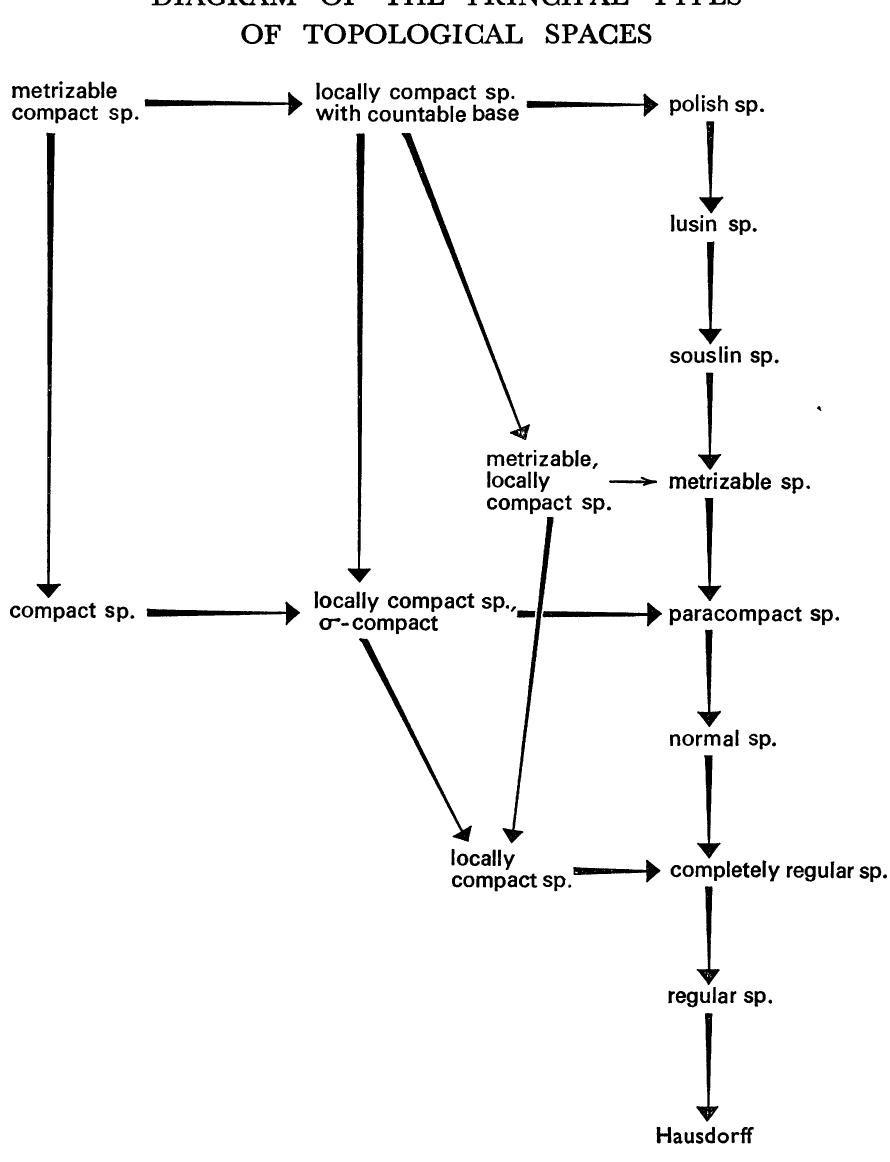
\includegraphics[keepaspectratio]{images/part002_2eb706e7.jpg}}

\section*{历史注记}
\phantomsection
\addcontentsline{toc}{section}{历史注记}

（括号中的数字指本注记末尾的参考文献。）

如我们在第 II 章的历史注记中所说，度量空间的概念是 M. Fréchet 于 1906 年引入的，几年后由 F. Hausdorff 在其``Mengenlehre''（《集论》）中加以发展。1920 年以后它获得了巨大的重要性，部分地是由于 S. Banach 及其学派关于赋范空间及其在泛函分析中的应用的基础性工作，也是由于绝对值概念在数论与代数几何中的重要性（在那里，关于一个绝对值的完备化过程特别地显示出是一种有力的工具）。

1920-1930 这十年间出现了一整系列关于度量空间性质的研究。这些由莫斯科学派进行的研究，特别着眼于寻求给定的拓扑可度量化的必要充分条件。这一思想运动凸显了正规空间概念的意义，该概念由 Tietze 于 1923 年定义，但其重要作用只是作为 Urysohn 关于连续实值函数扩张的工作{[}6{]}的结果才被认识到。除去单实变量函数这一平凡情形外，把定义在闭集上的连续实值函数扩张到整个空间的问题，最先（就平面的情形）由 H. Lebesgue{[}3{]}考虑；在 Urysohn 的决定性结果之前，它已由 H. Tietze{[}4{]}对度量空间解决。把这问题推广到取值于任意拓扑空间的函数，近年来在代数拓扑中获得了相当的重要性。最近的工作还表明，在这类问题中正规空间的概念不易处理，因为它容许太多``病态''的可能；它常常必须用更受限制的仿紧性概念来代替，后者是 J. Dieudonné 于 1944 年引入的{[}9{]}。在这一理论中，最值得注意的结果是 A. H. Stone 的定理{[}10{]}：每个可度量化空间都是仿紧的 (*)。

我们已经指出过（第 IV 章的历史注记），十九世纪末与二十世纪初（E. Borel、Baire、Lebesgue、Osgood、W. H. Young）关于 \(R^{n}\) 中点集的分类，以及关于通过迭代取极限过程（关于函数列）从连续函数得到的实值函数的分类与刻画的重要工作。人们很快认识到，度量空间——其 1910 年以后的发展主要是俄国与波兰学派的工作——构成了这类研究的自然领域。除其他方面外，度量空间的研究清楚地表明了贫集概念以及完备度量空间中稠密开集的可数交定理（ \(§\ 5,\ no.\ 3,\ Theorem\ 1\) ）在现代分析中所起的基本作用，该定理最先（相互独立地）由 Osgood{[}1{]}对实直线证明，并由 Baire{[}2{]}对空间 \(R^{n}\) 证明。

另一方面，Souslin 于 1917 年{[}5{]}在纠正 Lebesgue 的一个错误时证明了波莱尔集的连续像未必是波莱尔集；这引导他定义并研究更大的一类集，此后称为``解析集''或``苏斯林集''。Souslin 早逝之后，这项工作特别由 N. Lusin（其思想曾启发 Souslin 的工作）与波兰数学家们（见{[}7{]}与{[}8{]}）继续推进。这些集如今的重要性在于它们对积分理论（在那里，由于它们的特殊性质，可以进行对任意可测集而言不可能的构造）以及现代位势论的应用；在位势论中，关于苏斯林集可容性的基本定理（最近由 G. Choquet{[}11{]}证明）已显示出在种种应用中的丰富内容。

\subsection*{参考文献}

{[}1{]} W. Osgood, Non-uniform convergence and the integration of series term by term, Amer. Journ. of Math., 19 (1897), pp.~155-190.

{[}2{]} R. BAIRE, Sur les fonctions de variables réelles, Ann. di Mat. (3), 3 (1899), p.~i.

{[}3{]} H. LEBESGUE, Sur le problème des Dirichlet, Rend. Circ. mat. di Palermo, 24 (1907), pp.~371-402.

{[}4{]} H. TIETZE, Über Funktionen, die auf einer abgeschlossenen Menge stetig sind, J. de Crelle, 145 (1915), pp.~9-14.

{[}5{]} M. SOUSLIN, Sur une définition des ensembles mesurables B sans nombres transfinis, C. R. Acad. Sci., 164 (1917), pp.~88-91.

{[}6{]} P. URYSOHN, Über die Mächtigkeit der zusammenhängenden Mengen, Math. Ann., 94 (1925), p.~262.

{[}7{]} N. Lusin, Leçons sur les ensembles analytiques et leurs applications, Paris (Gauthier-Villars), 1930.

{[}8{]} K. KURATOWSKI, Topologie I, 2nd edition, Warszawa-Vrocaw, 1948.

{[}9{]} J. DIEUDONNÉ, Une généralisation des espaces compacts, Journ. de Math. (9), 23 (1944), pp.~65-76.

{[}10{]} A. H. STONE, Paracompactness and product spaces, Bull. Amer. Math. Soc., 54 (1948), pp.~977-982.

{[}11{]} G. CHOQUET, Theory of capacities, Ann. Inst. Fourier, 5 (1953-1954) pp.~131-295.

\ResumeMainChapters
\chapter{函数空间}

\section{\texorpdfstring{\(\mathfrak{S}\)-收敛的一致结构}{S-收敛的一致结构}}

记号。若 X 与 Y 是任意两个集，我们回忆 X 到 Y 的一切映射组成的集记作 \(\mathcal{F}(\mathbf{X};\mathbf{Y})\)，它可与乘积集 \(\mathbf{Y}^{\mathbf{x}}\) 等同（《集合论》，第 II 章，§ 5，第 2 号）。对 \(\mathcal{F}(\mathbf{X};\mathbf{Y})\) 的每个子集 H 与每个 \(x\in \mathbf{X}\)，我们将用 \(\mathrm{H}(x)\) 表示元素 \(u(x)\in \mathbf{Y}\)（当 \(u\) 取遍 H 时）组成的集。若 \(\Phi\) 是 \(\mathcal{F}(\mathbf{X};\mathbf{Y})\) 上的滤子基，我们用 \(\Phi (x)\) 表示由诸集 \(\mathrm{H}(x)\)（H 取遍 \(\Phi\)）组成的 Y 上的滤子基。最后，我们回忆，对每个 \(u\in \mathcal{F}(\mathbf{X};\mathbf{Y})\) 与 X 的每个子集 A，\(u|\mathrm{A}\) 表示 \(u\) 在 A 上的限制，它是 A 到 Y 中的映射；若 H 是 \(\mathcal{F}(\mathbf{X};\mathbf{Y})\) 的子集，则 H\textbar A 将表示限制 \(u|\mathrm{A}\)（函数 \(u\in \mathrm{H}\) 的）组成的集。

\subsection{一致收敛的一致结构}

设 X 是一个集，Y 是一致空间。对 Y 的每个围域 V，用 \(W(V)\) 表示 X 到 Y 中的映射的对 \((u, v)\) 中使 \((u(x), v(x)) \in V\)（对所有 \(x \in X\)）者组成的集。当 V 取遍 Y 的围域集时，诸集 \(W(V)\) 构成 F(X; Y) 上某个一致结构的围域基本系。因为它们显然满足公理 \((\mathrm{U}_{\mathrm{I}}^{\prime})\)（第 II 章，§ 1，第 1 号）；若 V 与 \(V'\) 是 Y 的两个使 \(V \subset V'\) 的围域，我们有 \(W(V) \subset W(V')\)，因而诸集 \(W(V)\) 满足 \((\mathrm{B}_{\mathrm{I}})\)（第 I 章，§ 6，第 3 号）；我们有 \(\widehat{W(V)} = W(\overline{V}^{-1})\)，故 \((\mathrm{U}_{\mathrm{II}}^{\prime})\) 满足；最后，关系式`` \((u(x), v(x)) \in V\)（对所有 \(x \in X\)）''与`` \((v(x), w(x)) \in V\)（对所有 \(x \in X\)）''蕴含关系式`` \((u(x), w(x)) \in V^{2}\)（对所有 \(x \in X\)）''；换言之，我们有 \(\widehat{W(V)} \subset W(\overline{V}^{2})\)，这就证明了 \((\mathrm{U}_{\mathrm{III}}^{\prime})\)。

定义 1 。在集 \(\mathcal{F}(\mathbf{X};\mathbf{Y})\) 上以子集 \(W(\mathbf{V})\)（其中 \(\mathbf{V}\) 取遍 \(\mathbf{Y}\) 的围域集）组成的集为围域基本系的一致结构，称为一致收敛的一致结构。它诱导的拓扑称为一致收敛的拓扑。若滤子 \(\Phi\)（\(\mathcal{F}(\mathbf{X};\mathbf{Y})\) 上的）关于这拓扑收敛于元素 \(u_0\)，则称 \(\Phi\) 一致收敛于 \(u_0\)。

注意 \(\mathcal{F}(\mathrm{X};\mathrm{Y})\) 上的一致收敛拓扑依赖于 Y 的一致结构，而不只是 Y 的拓扑（习题 4）。

把 \(\mathcal{F}(\mathbf{X};\mathbf{Y})\) 赋以一致收敛的一致结构所得的一致空间记作 \(\mathcal{F}_u(\mathbf{X};\mathbf{Y})\)。

\subsection{\texorpdfstring{\(\mathfrak{S}\)-收敛}{S-收敛}}

定义 2 。设 X 是一个集，Y 是一致空间，S 是 X 的子集组成的一个集。在 S 的集上一致收敛的一致结构，或简称 S-收敛的一致结构，是 F(X; Y) 上使限制映射 \(u \to u|A\)（F(X, Y) 到一致空间 \(\mathcal{F}_u(A; Y)\) 中的，其中 A 取遍 S）一致连续的最粗一致结构。把 F(X; Y) 赋以 S-收敛的一致结构所得的一致空间记作 \(\mathcal{F}_{\mathfrak{S}}(X; Y)\)。

\(\mathfrak{S}\)-收敛的一致结构所诱导的拓扑称为 \(\mathfrak{S}\)-收敛的拓扑；它是使所有映射 \(u \to u|A\)（\(\mathcal{F}(X; Y)\) 到 \(\mathcal{F}_u(A; Y) (A \in \mathfrak{S})\) 中的）都连续的最粗拓扑（第 II 章，§ 2，第 3 号，命题 4 的推论）。

滤子 \(\Phi\)（\(\mathcal{F}(\mathbf{X};\mathbf{Y})\) 上的）收敛于 \(u_{0}\)（关于 \(\mathfrak{S}\)-收敛的拓扑），当且仅当 \(u|\mathrm{A}\) 一致收敛于 \(u_{0}|\mathrm{A}\)（关于 \(\Phi\)，对所有 \(\mathrm{A}\in \mathfrak{S}\)）（第 I 章，§ 7，第 6 号，命题 10），因此称 \(\Phi\) 一致收敛于 \(u_{0}\)（在 \(\mathfrak{S}\) 的集上）。

滤子基 \(\Phi\)（\(\mathcal{F}_{\mathfrak{S}}(\mathbf{X};\mathbf{Y})\) 上的）是柯西滤子基，当且仅当对每个 \(\mathbf{A}\in\mathfrak{S}\)，\(\Phi\) 在映射 \(u\to u|\mathbf{A}\) 下的像是 \(\mathcal{F}_{u}(\mathbf{A};\mathbf{Y})\) 上的柯西滤子基（第 II 章，§ 3，第 1 号，命题 4）。

设 \(f\) 是拓扑（相应地，一致）空间 \(Z\) 到 \(\mathcal{F}_{\mathfrak{S}}(X; Y)\) 中的映射。则 \(f\) 连续（相应地，一致连续），当且仅当对每个 \(A \in \mathfrak{S}\)，映射 \(z \to f(z)|A\)（\(Z\) 到 \(\mathcal{F}_u(A; Y)\) 中的）连续（相应地，一致连续）（第 I 章，§ 2，第 3 号，命题 4；第 II 章，§ 2，第 3 号，命题 4）。

最后，设 \(\mathbf{M}\) 是 \(\mathcal{F}_{\mathfrak{S}}(\mathbf{X};\mathbf{Y})\) 的子集；则 \(\mathbf{M}\) 是准紧的，当且仅当对每个 \(\mathbf{A} \in \mathfrak{S}\)，限制 \(u|\mathbf{A}\)（\(u \in \mathbf{M}\)）组成的集是 \(\mathcal{F}_u(\mathbf{A};\mathbf{Y})\) 的准紧子集（第 II 章，§ 4，第 2 号，命题 3）。

注记。1) 初始一致结构的围域的一般定义（第 II 章，§ 2，第 3 号，命题 4）表明，\(\mathcal{F}_{\mathfrak{S}}(\mathrm{X};\mathrm{Y})\) 的围域基本系可如下得到：对每个 \(\mathbf{A}\in \mathfrak{S}\) 与每个围域 \(\mathbf{V}\)（\(\mathfrak{B}\) 的，此基本系属于 \(\mathbf{Y}\)），用 \(W(\mathbf{A},\mathbf{V})\) 表示映射的对 \((u,v)\)（\(\mathbf{X}\) 到 \(\mathbf{Y}\) 中的）中使 \((u(x),v(x))\in \mathbf{V}\)（对每个 \(x\in \mathbf{A}\)）者组成的集；当 \(\mathbf{A}\) 取遍 \(\mathfrak{S}\) 且 \(\mathbf{V}\) 取遍 \(\mathfrak{B}\) 时，诸集 \(W(\mathbf{A},\mathbf{V})\) 的有限交构成 \(\mathcal{F}_{\mathfrak{S}}(\mathrm{X};\mathrm{Y})\) 的围域基本系。

这描述立即表明：若 \(\mathfrak{S},\mathfrak{S}'\) 是 \(\mathbf{X}\) 的子集的两个集，使 \(\mathfrak{S} \subset \mathfrak{S}'\)，则 \(\mathfrak{S}'\)-收敛的一致结构比 \(\mathfrak{S}\)-收敛的一致结构更细。

\begin{enumerate}
\def\labelenumi{\arabic{enumi})}
\setcounter{enumi}{1}
\tightlist
\item
  然而，把 \(\mathfrak{S}\) 换成由含于 \(\mathfrak{S}\) 的集的有限并之中的 X 的所有子集组成的集 \(\mathfrak{S}'\)，\(\mathfrak{S}\)-收敛的一致结构不变。因此在研究 \(\mathfrak{S}\)-收敛时，我们总可以限于集 \(\mathfrak{S}\) 满足下列两个条件的情形：
\end{enumerate}

\((\mathbf{F}_{\mathbf{I}}^{\prime})\) \(\mathfrak{S}\) 中的集的每个子集都属于 \(\mathfrak{S}\)。

\((F_{\mathrm{II}}^{\prime})\) \(\mathfrak{S}\) 中的集的每个有限并都属于 \(\mathfrak{S}\)。

若 \((\mathbf{F}_{\mathrm{II}}^{\prime})\) 满足，则 \(\mathcal{F}_{\mathfrak{S}}(\mathbf{X};\mathbf{Y})\) 的一个围域基本系可这样得到：取所有集 \(\boldsymbol{W}(\mathrm{A},\mathrm{V})\)（其中 A 取遍 S，V 取遍 Y 的一个围域基本系）。

\begin{enumerate}
\def\labelenumi{\arabic{enumi})}
\setcounter{enumi}{2}
\tightlist
\item
  \(\mathfrak{S}\)-收敛的一致结构是这乘积空间的一致结构在映射 \(u \to (u|\mathbf{A})_{\mathbf{A} \in \mathfrak{S}}\)（\(\mathcal{F}(\mathbf{X}; \mathbf{Y})\) 到 \(\prod_{\mathbf{A} \in \mathfrak{S}} \mathcal{F}_u(\mathbf{A}; \mathbf{Y})\) 中的）下的逆像（第 II 章，§ 2，第 6 号，命题 8）。若 \(\mathfrak{S}\) 是 \(\mathbf{X}\) 的覆盖，则此映射是单射，因而 \(\mathcal{F}_{\mathfrak{S}}(\mathbf{X}; \mathbf{Y})\) 同构于 \(\prod_{\mathbf{A} \in \mathfrak{S}} \mathcal{F}_u(\mathbf{A}; \mathbf{Y})\) 的、作为此映射之像的一致子空间。
\end{enumerate}

命题 1 。若 Y 是豪斯多夫的且 S 是 X 的覆盖，则空间 \(\mathcal{F}_{\mathfrak{S}}(X;Y)\) 是豪斯多夫的。

设 \(u, v\) 是 \(\mathcal{F}_{\mathfrak{S}}(\mathrm{X}; \mathrm{Y})\) 的两个元素，使 \((u, v) \in W(\mathrm{A}, \mathrm{V})\)（对每个围域 \(\mathrm{V}\)（\(\mathrm{Y}\) 的）与每个 \(\mathrm{A} \in \mathfrak{S}\)）。由于 \(\mathrm{Y}\) 是豪斯多夫的，推出 \(u\) 与 \(v\) 在每个集 \(\mathrm{A} \in \mathfrak{S}\) 上一致；又因 \(\mathfrak{S}\) 覆盖 \(\mathrm{X}\)，必有 \(u = v\)。

注记。4) 设 H 是 \(\mathcal{F}(\mathbf{X};\mathbf{Y})\) 的子集。滥用术语，把 \(\mathfrak{S}\)-收敛的一致结构（相应地，拓扑）（\(\mathcal{F}(\mathbf{X};\mathbf{Y})\) 上的）在 H 上诱导的一致结构（相应地，拓扑）称为集 H 上 \(\mathfrak{S}\)-收敛的一致结构（相应地，拓扑）。

\begin{enumerate}
\def\labelenumi{\arabic{enumi})}
\setcounter{enumi}{4}
\tightlist
\item
  设 L 是由滤子 \(\mathfrak{G}\) 滤化的集，且 \(\lambda \to u_{\lambda}\) 是 L 到 \(\mathcal{F}_{\mathfrak{S}}(\mathbf{X};\mathbf{Y})\) 中的、有极限 \(v\)（关于 \(\mathfrak{G}\)）的映射；这时我们说，关于滤子 \(\mathfrak{G}\)，X 到 Y 中的映射 \(u_{\lambda}\) 一致收敛于 \(v\){[}或族 \((u_{\lambda})\) 一致收敛于 \(v\){]}（在 \(\mathfrak{S}\) 的每个集上）。若 \(\mathbf{L} = \mathbf{N}\) 且 \(\mathfrak{G}\) 是弗雷歇滤子，则在这陈述中省略对 \(\mathfrak{G}\) 的提及。
\end{enumerate}

更特殊地，设 Y 上定义了一个交换且结合的、以加法记号书写的合成律。若 \((u_{n})\) 是 X 到 Y 中的映射的任一序列，用 \(v_{n}\) 表示由下式定义的映射

\[
v _ {n} (x) = \sum_ {k = 0} ^ {n} u _ {k} (x) \quad (n \in \mathbf {N});
\]

我们说以 \(u_n\) 为通项的级数在 \(\mathfrak{S}\) 的每个集上一致收敛，如果序列 \((v_n)\) 在 \(\mathfrak{S}\) 的每个集上一致收敛。类似地，映射的一致可和族 \((u_\lambda)_{\lambda \in \mathbf{L}}\)（\(\mathbf{X}\) 到 \(\mathbf{Y}\) 中的）通过考虑映射 \(x \to \sum_{\lambda \in \mathbf{J}} u_\lambda(x)\)（对 L 的所有有限子集

J）以及这些映射在 \(\mathcal{F}_{\mathfrak{S}}(\mathbf{X};\mathbf{Y})\) 中关于 L 的有限子集的定向集的极限来定义（第 III 章，§ 5，第 1 号）。

\begin{enumerate}
\def\labelenumi{\arabic{enumi})}
\setcounter{enumi}{5}
\tightlist
\item
  由定义 1 与定义 2 立即得出：对每个 \(x \in \bigcup_{\mathbf{A} \in \mathfrak{S}} \mathbf{A}\)，映射 \(u \to v(x)\)（\(\mathcal{F}_{\mathfrak{S}}(\mathbf{X}; \mathbf{Y})\) 到 Y 中的）是一致连续的。因而特别地，若用 \(\overline{\mathbf{H}}\) 表示 \(\mathcal{F}_{\mathfrak{S}}(\mathbf{X}; \mathbf{Y})\) 的子集 H 的闭包，则有 \(\overline{\mathbf{H}}(x) \subset \overline{\mathbf{H}(x)}\)（对所有 \(x \in \bigcup_{\mathbf{A} \in \mathfrak{S}} \mathbf{A}\)）（第 I 章，§ 2，第 1 号，定理 1）。
\end{enumerate}

\subsection{\texorpdfstring{\(\mathfrak{S}\)-收敛的例子}{S-收敛的例子}}

I. 在 X 的子集上的一致收敛。设 A 是 X 的子集，取 \(\mathfrak{S} = \{\mathrm{A}\}\)。\(\mathfrak{S}\)-收敛的一致结构（相应地，拓扑）这时称为在 A 中一致收敛的一致结构（相应地，拓扑）；若滤子 \(\Phi\)（\(\mathcal{F}_{\mathfrak{S}}(\mathrm{X};\mathrm{Y})\) 上的）收敛于 \(u_0\)，则称它在 A 中一致收敛于 \(u_0\)。当 \(\mathrm{A} = \mathrm{X}\) 时，我们重新得到第 1 号中定义的一致收敛结构。

\begin{enumerate}
\def\labelenumi{\Roman{enumi}.}
\setcounter{enumi}{1}
\tightlist
\item
  在 X 的子集上的逐点收敛。设 A 是 X 的子集，取 S 为由属于 A 的单个点组成的 X 的所有子集之集（由第 2 号的注记 2，若取 S 为 A 的所有有限子集之集，效果相同）。S-收敛的一致结构（相应地，拓扑）这时称为在 A 中逐点收敛的一致结构（相应地，拓扑）；若 \(\mathcal{F}_{\mathfrak{S}}(\mathbf{X};\mathbf{Y})\) 上的滤子 Φ 收敛于 \(u_0\)，则称它在 A 中逐点收敛于 \(u_0\)。这种情形成立当且仅当：对每个 \(x\in \mathbf{A}\)，\(u_0(x)\) 是 \(u(x)\) 关于滤子 Φ 的极限。
\end{enumerate}

特别地，当 A = X 时，在 X 中逐点收敛的一致结构（相应地，拓扑）就简称为逐点收敛的一致结构（相应地，拓扑）；把 \(\mathcal{F}(X; Y)\) 赋以这结构所得的一致空间记作 \(\mathcal{F}_{s}(X; Y)\)。注意逐点收敛的拓扑就是 \(Y^{X}\) 上的乘积拓扑，因而只依赖于 Y 的拓扑而不依赖其一致结构。

\begin{enumerate}
\def\labelenumi{\Roman{enumi}.}
\setcounter{enumi}{2}
\tightlist
\item
  紧收敛。设 X 是拓扑空间，取 S 为 X 的所有紧子集组成的集。这时 S-收敛的一致结构（相应地，拓扑）称为紧收敛的一致结构（相应地，拓扑），而赋予 \(\mathcal{F}(X;Y)\) 此一致结构所得的一致空间记作 \(\mathcal{F}_{c}(X;Y)\)。紧收敛的结构比一致收敛的结构粗，且当 X 紧时二者一致；它又比逐点收敛的结构细，且当 X 离散时这二者一致。
\end{enumerate}

若 X 是一致空间，则通过取 S 为 X 的所有准紧子集组成的集，我们可以在 \(\mathcal{F}(X;Y)\) 上定义准紧收敛的一致结构。同样，若 X 是度量空间，则可取 S 为 X 的所有有界子集组成的集；这时 S-收敛的一致结构称为有界收敛的一致结构。

\subsection{\texorpdfstring{空间 \(\mathcal{F}_{\mathfrak{G}}(\mathbf{X};\mathbf{Y})\) 的性质}{空间 F 下标 G (X;Y) 的性质}}

命题 2. 设 \(\mathbf{X}_1, \mathbf{X}_2\) 是两个集，\(\mathbf{Y}\) 是一致空间，\(\mathfrak{S}_i\) 是 \(\mathbf{X}_i\) 的子集组成的集（\(i = 1, 2\)），而 \(\mathfrak{S}_1 \times \mathfrak{S}_2\) 是 \(\mathbf{X}_1 \times \mathbf{X}_2\) 的形如 \(\mathbf{A}_1 \times \mathbf{A}_2\) 的子集组成的集，其中 \(\mathbf{A}_i \in \mathfrak{S}_i\)（\(i = 1, 2\)）。则典范双映射

\[
\mathscr {F} \left(\mathrm{X} _ {1} \times \mathrm{X} _ {2}; \mathrm{Y}\right)\rightarrow \mathscr {F} \left(\mathrm{X} _ {1}; \mathscr {F} \left(\mathrm{X} _ {2}; \mathrm{Y}\right)\right)
\]

（集合论，R，§ 4，第 14 号）是一致空间

\[
\mathcal {F} _ {\mathfrak {S} _ {1} \times \mathfrak {S} _ {2}} (\mathrm{X} _ {1} \times \mathrm{X} _ {2}; \mathrm{Y})
\]

到 \(\mathcal{F}_{\mathfrak{S}_1}(\mathbf{X}_1;\mathcal{F}_{\mathfrak{S}_2}(\mathbf{X}_2;\mathbf{Y}))\) 上的同构

设 \(\mathbf{V}\) 是 \(\mathbf{Y}\) 的围域，\(\mathbf{A}_i\in \mathfrak{S}_i\)（\(i = 1,2\)）；则由定义立即可见，\(W(\mathbf{A}_1\times \mathbf{A}_2,\mathbf{V})\) 经典范双映射与 \(W(\mathbf{A}_1,W(\mathbf{A}_2,\mathbf{V}))\) 等同，结论立得。

命题 3. a) 设 X 是一个集；S 是 X 的子集组成的一个集；Y、Y' 是两个一致空间；f: Y → Y' 是一致连续映射。则 F\_S(X; Y) 到 F\_S(X; Y') 中的映射 u → f ∘ u 是一致连续的。

\begin{enumerate}
\def\labelenumi{\alph{enumi})}
\setcounter{enumi}{1}
\tightlist
\item
  设 \(\mathbf{X}, \mathbf{X}'\) 是两个集；\(\mathfrak{S}\)（相应地，\(\mathfrak{S}'\)）是 \(\mathbf{X}\)（相应地，\(\mathbf{X}'\)）的子集组成的集；\(\mathbf{Y}\) 是一致空间；\(g: \mathbf{X}' \to \mathbf{X}\) 是这样的映射：对每个 \(\mathbf{A}' \in \mathfrak{S}'\)，\(g(\mathbf{A}')\) 含于 \(\mathfrak{S}\) 中集的有限并。则映射 \(u \to u \circ g\)（\(\mathcal{F}_{\mathfrak{S}}(\mathbf{X}, \mathbf{Y})\) 到 \(\mathcal{F}_{\mathfrak{S}'}(\mathbf{X}', \mathbf{Y})\) 中的）是一致连续的。
\end{enumerate}

命题 4. 设 X、Y 是两个集，\((\mathbf{X}_{\lambda})_{\lambda \in \mathbf{L}}\) 是一个集族，\((\mathrm{Y}_{\mu})_{\mu \in \mathbf{M}}\) 是一个一致空间族。对每个 \(\lambda \in \mathbf{L}\)，设 \(\mathfrak{S}_{\lambda}\) 是 \(\mathbf{X}_{\lambda}\) 的子集组成的集，\(g_{\lambda}\) 是 \(\mathbf{X}_{\lambda}\) 到 X 中的映射，而 \(\mathfrak{S}\) 是 X 的子集组成的集，即诸集 \(g_{\lambda}(\mathfrak{S}_{\lambda})\) 的并。对每个 \(\mu \in \mathbf{M}\)，设 \(f_{\mu}\) 是 Y 到 \(Y_{\mu}\) 中的映射，并赋予 Y 使诸 \(f_{\mu}\) 都一致连续的最粗一致结构。则 \(\mathcal{F}(X;Y)\) 上 S-收敛的一致结构是使映射 \(u \to f_{\mu} \circ u \circ g_{\lambda}\)（\(\mathcal{F}(X;Y)\) 到 \(\mathcal{F}_{\mathfrak{S}_{\lambda}}(X_{\lambda},Y_{\mu})\) 中的）都一致连续的最粗一致结构。

这些命题是第 2 号注记 1 中给出的 S-收敛的一致结构的围域基本系描述的直接推论；证明的细节留给读者。特别地，命题 4 蕴含：

推论. 设 X 是一个集，\((\mathrm{Y}_{t})_{t\in\mathbf{I}}\) 是一致空间族，S 是 X 的子集组成的集。若赋予 \(\prod_{t\in I}Y_{t}\) 乘积一致结构，则一致空间 \(\mathcal{F}_{\mathfrak{S}}\left(\mathrm{X},\prod_{t\in\mathbf{I}}\mathrm{Y}_{t}\right)\) 到乘积一致空间 \(\prod_{t\in\mathbf{I}}\mathcal{F}_{\mathfrak{S}}(\mathrm{X};\mathrm{Y}_{t})\) 上的典范双映射（集合论，R，§ 4，第 13 号）是同构。

\subsection{\texorpdfstring{\(\mathcal{F}_{\mathfrak{S}}(\mathbf{X};\mathbf{Y})\) 的完全子集}{F 下标 S (X;Y) 的完全子集}}

命题 5. 设 \(\Phi\) 是一个集，Y 是一致空间，\(\mathfrak{S}\) 是 X 的子集组成的集。则滤子 \(\Phi\)（\(\mathcal{F}_{\mathfrak{S}}(\mathbf{X};\mathbf{Y})\) 上的）收敛于 \(u_0\) 的充要条件是：\(\Phi\) 是关于 \(\mathfrak{S}\) -收敛的一致结构的柯西滤子，且逐点收敛于 \(u_0\)（在 \(\mathbf{B} = \bigcup_{\mathbf{A}\in \mathfrak{S}}\mathbf{A}\) 中）。

由于 B 中逐点收敛的结构比 S-收敛的结构粗，只需证明：对每个 \(A \in S\) 与 Y 的每个闭围域 V，\(W(A, V)\) 关于逐点收敛拓扑在 B 中是闭的（第 II 章，§ 3，第 3 号，命题 7）。而 \(W(A, V)\) 是诸映射 \((u, v) \to (u(x), v(x))\)（当 x 取遍 A 时）下 V 的原象的交；这些映射关于逐点收敛拓扑连续（第 2 号注记 6），由此即得结论。

推论 1. \(\mathcal{F}_{\mathfrak{S}}(\mathbf{X};\mathbf{Y})\) 的子空间 H 是完全的，充要条件是：对 H 上每个柯西滤子 \(\Phi\)，存在 \(u_0\in \mathbf{H}\)，使 \(\Phi\) 逐点收敛于 \(u_0\)（在 \(\mathbf{B} = \bigcup_{\mathbf{A}\in \mathfrak{S}}\mathbf{A}\) 中）。

这由命题 5 立得。

推论 2. 设 \(\mathfrak{S}_1, \mathfrak{S}_2\) 是 X 的子集组成的两个集，它们的并相同，且 \(\mathfrak{S}_1 \subset \mathfrak{S}_2\)，又设 H 是 \(\mathcal{F}(X; Y)\) 的子集。则若 H 关于 \(\mathfrak{S}_1\) -收敛是完全的，它关于 \(\mathfrak{S}_2\) -收敛也是完全的。

因为关于 \(S_{2}\) -收敛的每个柯西滤子也是关于 \(S_{1}\) -收敛的柯西滤子，故可应用推论 1。

推论 3. 设 H 是 \(\mathcal{F}(\mathbf{X};\mathbf{Y})\) 的子集，使得对每个

\[
x \notin \mathrm{B} = \bigcup_ {\mathrm{A} \in \mathfrak {S}} \mathrm{A},
\]

\(\mathbf{H}(x)\) 在 \(\mathbf{Y}\) 中的闭包是 \(\mathbf{Y}\) 的完全子空间。则 \(\overline{\mathbf{H}}\)（即 \(\mathbf{H}\) 在 \(\mathcal{F}_{\mathfrak{S}}(\mathbf{X};\mathbf{Y})\) 中的闭包）是完全子空间。

设 \(\Phi\) 是 \(\overline{\mathbf{H}}\) 上的柯西滤子，如下定义映射 \(v: \mathbf{X} \to \mathbf{Y}\)。若 \(x \in \mathbf{B}\)，则 \(\Phi(x)\) 是 \(\overline{\mathbf{H}(x)}\) 上的柯西滤子（第 2 号注记 6），故由假设它至少有一个极限点；取 \(v(x)\) 为这些极限之一。若 \(x \notin \mathbf{B}\)，取 \(v(x)\) 为 \(\mathbf{Y}\) 的任意一点。以如此定义的 \(v\)，显然 \(\Phi\) 逐点收敛于 \(v\)（在 \(\mathbf{B}\) 中），因而由命题 5，\(v\) 是 \(\Phi\) 在 \(\mathcal{F}_{\mathfrak{S}}(\mathbf{X}; \mathbf{Y})\) 中的一个极限。

特别地，若 Y 是完全的，则命题 5 的推论 3 的假设对每个 \(H \subset \mathcal{F}(X; Y)\) 都满足；因此：

定理 1. 设 X 是一个集，S 是 X 的子集组成的一个集，Y 是完全一致空间。则一致空间 \(\mathcal{F}_{\mathfrak{S}}(X;Y)\) 是完全的。

\subsection{\texorpdfstring{连续映射空间中的 \(\mathfrak{S}\)-收敛}{连续映射空间中的 S-收敛}}

设 X、Y 为两个拓扑空间，用 C(X; Y) 表示由 X 到 Y 中的全体连续映射所成之集。若 S 是 X 的子集所成之集，且 Y 是一致空间，则用 \(\mathcal{C}_{\mathfrak{S}}(\mathbf{X};\mathbf{Y})\) 表示赋有 S-收敛一致结构的集合 C(X; Y)。特别地，\(\mathcal{C}_{s}(\mathbf{X};\mathbf{Y})\) 、\(\mathcal{C}_{c}(\mathbf{X};\mathbf{Y})\) 与 \(\mathcal{C}_{u}(\mathbf{X};\mathbf{Y})\) 分别表示赋有逐点收敛、紧收敛与一致收敛一致结构的集合 C(X; Y)。

命题 6. 设 X 是拓扑空间，Y 是一致空间，S 是 X 的子集所成之集。对每个 A ∈ S 以及 Y 的每个闭围域 V，W(A, V) 与 W(A̅, V) 在 C (X; Y) × C (X; Y) 上的迹相同。

因为若 \(u, v\) 是 \(\mathbf{X}\) 到 \(\mathbf{Y}\) 中的连续映射，则映射 \(x \to (u(x), v(x))\) 把 \(\mathbf{X}\) 映入 \(\mathbf{Y} \times \mathbf{Y}\) 并且连续，于是由 \((u(x), v(x)) \in \mathbf{V}\) 对一切 \(x \in \mathbf{A}\) 成立这一假设便可推出，\((u(x), v(x)) \in \overline{\mathbf{V}} = \mathbf{V}\) 对一切 \(x \in \overline{\mathbf{A}}\) 成立（第 I 章，§ 2，第 1 号，定理 1）。

若用 \(\overline{\mathfrak{S}}\) 表示在 \(\mathbf{X}\) 中所取的 \(\mathfrak{S}\) 的诸集的闭包所成之集，则命题 6 表明，在 \(\mathcal{C}(\mathbf{X};\mathbf{Y})\) 上，\(\mathfrak{S}\) -收敛与 \(\overline{\mathfrak{S}}\) -收敛的结构相同。

推论. 设 B 是 X 的稠密子集。在 C(X; Y) 上，一致收敛的结构与 B 上的一致收敛的结构相同。

命题 7. 设 X 是拓扑空间，S 是 X 的子集所成之集，Y 是一致空间。若 Y 是豪斯多夫空间，且 S 中诸集的并 B 在 X 中稠密，则 \(\mathcal{C}_{\mathfrak{S}}(X;Y)\) 是豪斯多夫空间。

因为若 \((u, v)\) 属于所有的集 \(W(A, V)\) ，其中 \(A \in \mathfrak{S}\) 而 \(V\) 取遍 \(Y\) 的围域，则由 \(Y\) 是豪斯多夫空间这一假设知，\(u(x) = v(x)\) 对一切 \(x \in B\) 成立；若 \(u\) 与 \(v\) 连续，则由恒等延拓原理得 \(u = v\)（第 I 章，§ 8，第 1 号，命题 2 的推论 1）。

特别地，在 \(\mathcal{C}(\mathbf{X};\mathbf{Y})\) 上，\(\mathbf{X}\) 的一个稠密子集上的逐点收敛拓扑是豪斯多夫的。

命题 8. 设 X 是一个集合，F 是 X 上的滤子，Y 是一致空间。则由映射 \(u: \mathbf{X} \to \mathbf{Y}\) （其中 \(u(\mathfrak{F})\) 是 Y 上的柯西滤子基）所成之集 H 在 \(\mathcal{F}_u(\mathbf{X}; \mathbf{Y})\) 中是闭的。

设 \(u_0: \mathbf{X} \to \mathbf{Y}\) 属于 \(\mathbf{H}\) 在 \(\mathcal{F}_u(\mathbf{X}; \mathbf{Y})\) 中的闭包。设 \(\mathbf{V}\) 为 \(\mathbf{Y}\) 的任一对称围域，则存在映射 \(u \in \mathbf{H}\) ，使得 \((u_0(x), u(x)) \in \mathbf{V}\) 对一切 \(x \in \mathbf{X}\) 成立；另一方面，由假设存在集 \(\mathbf{M} \in \mathfrak{F}\) ，使得 \((u(x), u(x')) \in \mathbf{V}\) 每当 \(x\) 与 \(x'\) 都属于 \(\mathbf{M}\) 。由于 \((u_0(x), u(x)) \in \mathbf{V}\) 且 \((u_0(x'), u(x')) \in \mathbf{V}\) ，便得 \((u_0(x), u_0(x')) \in \overset{3}{\mathbf{V}}\) 每当 \(x\) 与 \(x'\) 都属于 \(\mathbf{M}\) ，从而 \(u_0(\mathfrak{F})\) 是 \(\mathbf{Y}\) 上的柯西滤子基。

推论 1. 设 X 是拓扑空间，Y 是一致空间。在一点 \(x_{0} \in X\) 处连续的、由 X 到 Y 中的映射所成之集在 \(\mathcal{F}_{u}(X; U)\) 中是闭的。

若 V 是 \(x_{0}\) 在 X 中的邻域滤子，则 \(u(x_{0})\) 是 \(u(\mathbf{V})\) 的接触点；因此 u 在 \(x_{0}\) 处连续当且仅当 \(u(\mathbf{V})\) 是 Y 上的柯西滤子基（第 II 章，§ 3，第 2 号，命题 5 的推论 2）。

推论 2. 设 X、L 为两个集合，分别带有滤子 F、G，并设 Y 是完备一致空间。对每个 \(\lambda \in L\) ，设 \(u_{\lambda}\) 是 X 到 Y 中的一个映射。假设：(i) 族 \((u_{\lambda})_{\lambda \in L}\) 在 X 中（关于滤子 G）一致收敛于映射 \(v: X \to Y\) ；(ii) 对每个 \(\lambda \in L\) ，\(u_{\lambda}\) 关于滤子 F 有极限 \(y_{\lambda}\) 。在这些条件下，\(v\) 关于 F 有极限，且 \(v\) 关于 F 的每个极限都是族 \((y_{\lambda})_{\lambda \in L}\) 关于 G 的极限。

因为 \(v\) 属于诸 \(u_{\lambda}\) 所成之集在 \(\mathcal{F}_u(\mathbf{X};\mathbf{Y})\) 中的闭包，故由命题 8 知 \(v(\mathfrak{F})\) 是 \(\mathbf{Y}\) 上的柯西滤子基；这表明 \(v\) 有极限 \(y\) （关于 \(\mathfrak{F}\) ），因为 \(\mathbf{Y}\) 是完备的。设

\(X' = X \cup \{\omega\}\) 为与滤子 \(\mathfrak{F}\) 相伴的拓扑空间（第 I 章，§ 6，第 5 号），并把 \(u_{\lambda}\) （相应地，\(v\) ）延拓为 \(\overline{u}_{\lambda}\) （相应地，\(\overline{v}\) ），即 \(X'\) 到 Y 中的映射，办法是令 \(\overline{u}_{\lambda}(\omega) = y_{\lambda}\) {[}相应地 \(\overline{v}(\omega) = y\) {]}。于是映射 \(\overline{u}_{\lambda}, \overline{v}\) 在 \(X'\) 上连续，且 \(\overline{u}_{\lambda}\) 在 X 中一致收敛于 \(\overline{v}\) （关于 \(\mathfrak{G}\) ）；由于 X 在 \(X'\) 中稠密，命题 6 的推论表明 \(\overline{u}_{\lambda}\) 在 \(X'\) 中一致收敛于 \(\overline{v}\) ，特别地有 \(y = \lim_{\mathfrak{G}} y_{\lambda}\) 。

定理 2. 设 X 是拓扑空间，Y 是一致空间。则由 X 到 Y 中的连续映射所成之集 C(X; Y) 是赋有一致收敛拓扑的空间 F(X; Y) 的闭子集。

对每个 \(x \in \mathbf{X}\) ，由 \(\mathbf{X}\) 到 \(\mathbf{Y}\) 中的、在 \(x\) 处连续的映射所成之集在 \(\mathcal{F}_u(\mathbf{X};\mathbf{Y})\) 中是闭的（命题 8 的推论 1）；因此这些集的交 \(\mathcal{C}(\mathbf{X};\mathbf{Y})\) 也是闭的。

这一结果可以表述为：连续函数的一致极限仍然连续。

推论 1. 若 Y 是完备一致空间，则 \(\mathcal{C}_{u}(\mathbf{X};\mathbf{Y})\) 是完备的。因为由定理 2，\(\mathcal{C}_{u}(\mathbf{X};\mathbf{Y})\) 是一致空间 \(\mathcal{F}_{u}(\mathbf{X};\mathbf{Y})\) 的闭一致子空间，而后者由第 5 号的定理 1 是完备的。

推论 2. 设 X 是拓扑空间，S 是 X 的子集所成之集，Y 是一致空间。用 \(\tilde{\mathcal{C}}_{\mathfrak{S}}(X;Y)\) 表示由其在 S 的每个集上的限制都连续的、X 到 Y 中的全体映射所成之集。则 \(\tilde{\mathcal{C}}_{\mathfrak{S}}(X;Y)\) 是一致空间 \(\mathcal{F}_{\mathfrak{S}}(X;Y)\) 的闭子空间，且当 Y 完备时它是完备的。

设 \(u\) 属于 \(\tilde{\mathcal{C}}_{\mathfrak{S}}(\mathbf{X};\mathbf{Y})\) 在 \(\mathcal{F}_{\mathfrak{S}}(\mathbf{X};\mathbf{Y})\) 中的闭包；则（第 2 号）对每个 \(\mathbf{A} \in \mathfrak{S}\) ，\(u|\mathbf{A}\) 属于 \(\mathcal{C}(\mathbf{A};\mathbf{Y})\) 在 \(\mathcal{F}_u(\mathbf{A};\mathbf{Y})\) 中的闭包，从而由定理 2 知它连续。

推论 3. 设 X 是可度量化或局部紧的拓扑空间，Y 是一致空间。则 \(\mathcal{C}(\mathbf{X};\mathbf{Y})\) 在一致空间 \(\mathcal{F}_c(\mathbf{X};\mathbf{Y})\) 中是闭的；若此外 Y 还是完备的，则一致空间 \(\mathcal{C}_c(\mathbf{X};\mathbf{Y})\) 是完备的。

由推论 2，只需证明：若取 \(\mathfrak{S}\) 为 X 的紧子集所成之集，则在所考虑的两种情形下都有 \(\tilde{\mathcal{C}}_{\mathfrak{S}}(X;Y) = \mathcal{C}(X;Y)\) 。若 X 局部紧，这是显然的。若 X 可度量化，且 \(u: X \to Y\) 是一个在每个紧子集上的限制都连续的映射，则对每个 \(x \in X\) 以及每个序列 \((z_n)\) （由 X 的点组成且收敛于 \(x\) ），有 \(u(x) = \lim_{n \to \infty} u(z_n)\) ，因此 \(u\) 在 \(x\) 处连续（第 IX 章，§ 2，第 6 号，命题 10）。

注意，只要 \(\mathbf{X}\) 的每一点都具有可数的基本邻域系，上面的论证就适用。

\pandocbounded{
\includegraphics[keepaspectratio]{images/part002_71b18b59.jpg}}

注。1) 一般说来，集 \(\mathcal{C}(\mathbf{X};\mathbf{Y})\) 关于逐点收敛拓扑在 \(\mathcal{F}(\mathbf{X};\mathbf{Y})\) 中不是闭的：换句话说，连续函数的逐点极限未必连续{[}习题 5 a){]}。

\begin{enumerate}
\def\labelenumi{\arabic{enumi})}
\setcounter{enumi}{1}
\tightlist
\item
  \(\mathcal{C}(\mathbf{X};\mathbf{Y})\) 上的一个滤子可以逐点收敛于一个连续函数而不一致收敛于这个函数。
\end{enumerate}

例如，在区间 I = {[}0, 1{]} 上，设 \(u_n\) 是这样的实值函数：当 \(x = 0\) 且 \(2/n \leqslant x \leqslant 1\) 时等于 0，当 \(x = 1/n\) 时等于 1，并且在区间 {[}0, 1/n{]} 与 {[}1/n, 2/n{]} 的每一个中都是线性的。序列 \((u_n)\) 逐点收敛于 0，但在 I 中不一致收敛于 0（参见习题 6）。

\begin{enumerate}
\def\labelenumi{\arabic{enumi})}
\setcounter{enumi}{2}
\item
  若 X 是一致空间，则与命题 8 类似的证明表明，由 X 到 Y 中的一致连续映射所成之集在 \(\mathcal{F}_u(X;Y)\) 中是闭的。
\item
  设一致空间 Y 带有一个交换且结合的合成律，用加法记写，使得映射 \((y, y') \to y + y'\) 在 \(Y \times Y\) 上连续。于是，若 \((u_n)\) 是 X 到 Y 中的连续映射序列，且以 \(u_n\) 为通项的级数在 X 中一致收敛，则该级数的和在 X 上连续。
\end{enumerate}

关于连续映射的一致可和族（第 1 号，注 5）的相应结果，留给读者自行叙述。

命题 9. 设 X 是拓扑空间，Y 是一致空间。则映射 \((f, x) \to f(x)\) （由 \(\mathcal{C}_u(X; Y) \times X\) 到 Y 中）是连续的。

设 \(f_0: \mathbf{X} \to \mathbf{Y}\) 是连续映射，\(x_0\) 是 \(\mathbf{X}\) 的一点，\(\mathbf{V}\) 是 \(\mathbf{Y}\) 的一个围域。集 \(\mathbf{T}\) 由诸连续映射 \(f: \mathbf{X} \to \mathbf{Y}\) 组成，它们满足 \((f(x), f(x_0)) \in \mathbf{V}\) 对一切 \(x \in \mathbf{X}\) 成立；这个集是 \(f_0\) 在 \(\mathcal{C}_u(\mathbf{X}; \mathbf{Y})\) 中的一个邻域。另一方面，由于 \(f_0\) 连续，存在一个邻域 \(\mathbf{U}\) （\(x_0\) 在 \(\mathbf{X}\) 中的邻域），使得 \((f_0(x), f_0(x_0)) \in \mathbf{V}\) 对一切 \(x \in \mathbf{U}\) 成立。因此我们有 \((f(x), f(x_0)) \in \overset{\circ}{\mathbf{V}}\) 每当 \((f, x) \in \mathbf{T} \times \mathbf{U}\) ，从而结论得证。

\section{等度连续集}

\subsection{定义与一般判别法}

定义 1. 设 X 是拓扑空间，Y 是一致空间。称 F(X; Y) 的子集 H 在一点 \(x_{0} \in X\) 处等度连续，如果对 Y 的每个围域 V，存在 \(x_{0}\) 在 X 中的邻域 U，使得 \((f(x_{0}),f(x))\in\mathbf{V}\) 对一切 \(x\in\mathbf{U}\) 及一切 \(f\in\mathbf{H}\) 成立。称 H 是等度连续的，如果它在 X 的每一点都等度连续。

定义 2. 设 X 与 Y 是两个一致空间。称 \(\mathcal{F}(X;Y)\) 的子集 H 是一致等度连续的，如果对 Y 的每个围域 V，存在 X 的围域 U，使得我们就有 \((f(x), f(x')) \in V\) ，只要 \((x, x') \in U\) 且 \(f \in H\) 。

称 X 到 Y 中的映射的族 \((f_{t})_{t\in I}\) 在一点 \(x_0\) 处等度连续（相应地，等度连续、一致等度连续），如果诸 \(f_{t}\) 所成之集在 \(x_0\) 处等度连续（相应地，等度连续、一致等度连续）。

显然，若 \(\mathbf{H}\subset\mathcal{F}(\mathbf{X};\mathbf{Y})\) 在 \(x_{0}\) 处等度连续，则每个 \(f\in H\) 在 \(x_{0}\) 处连续；若 H 等度连续，则每个 \(f\in H\) 在 X 上连续，即 \(\mathbf{H}\subset\mathcal{C}(\mathbf{X};\mathbf{Y})\) 。同样，若 H 一致等度连续（X 是一致空间），则每个 \(f\in H\) 在 X 上一致连续。同样显然的是，一致等度连续的映射集是等度连续的；但一个由一致连续映射组成的集可以是等度连续的而非一致等度连续的（见习题 1；命题 1 的推论 2；以及第 2 号的命题 4）。

例。1) 设 X 是拓扑空间（相应地，一致空间），Y 是一致空间。由 X 到 Y 中的连续（相应地，一致连续）映射所成的每个有限集都是等度连续（相应地，一致等度连续）的。

\begin{enumerate}
\def\labelenumi{\arabic{enumi})}
\setcounter{enumi}{1}
\tightlist
\item
  设 X、Y 是两个度量空间，d（相应地，d'）是 X（相应地，Y）上的度量，并设 k、\(\alpha\) 是两个实数 \textgreater{} 0。则使
\end{enumerate}

\[
d ^ {\prime} (f (x), f (x ^ {\prime})) \leqslant k (d (x, x ^ {\prime})) ^ {\alpha}
\]

对每一对点 \(x, x'\) （属于 \(\mathbf{X}\) ）都成立的全体映射 f: X → Y 所成之集是一致等度连续的。例如，\(\mathbf{X}\) 到 \(\mathbf{Y}\) 的一个子集上的全体等距映射（第 IX 章，§ 2，第 2 号）是一致等度连续的。

* 设 H 是定义在区间 I ⊂ R 上的实值函数所成之集，这些函数在 I 上可微，且满足 \(|f'(x)| \leqslant k\) 对所有 \(x \in I\) 及所有 \(f \in H\) 成立。则 H 是一致等度连续的，因为若 \(x_{1}, x_{2}\) 是 I 的任意两点，则由中值定理，有 \(|f(x_{1}) - f(x_{2})| \leqslant k |x_{1} - x_{2}|\) 对每个 \(f \in H\) 成立。 *

\begin{enumerate}
\def\labelenumi{\arabic{enumi})}
\setcounter{enumi}{2}
\tightlist
\item
  设 G 是拓扑群，Y 是一致空间，\(f: \mathbf{G} \to \mathbf{Y}\) 是一致连续映射{[}G 赋有它的左一致结构（第 III 章，§ 3，第 1 号）{]}。对每个 \(s \in \mathbf{G}\) ，用 \(f_s\) 表示 G 到 Y 中的映射 \(x \to f(sx)\) 。则诸映射 \(f_s(s \in \mathbf{G})\) 所成之集是一致等度连续的，因为关系 \(x^{-1}x' \in V\) 等价于 \((sx)^{-1}(sx') \in V\) 。
\end{enumerate}

命题 1. 设 T 是一个集合，S 是 T 的子集所成之集，Y 是一致空间，X 是拓扑（相应地，一致）空间，f 是 \(\mathbf{T} \times \mathbf{X}\) 到 \(\mathbf{Y}\) 中的一个映射。对每个 \(\mathbf{A} \in \mathfrak{S}\) ，用 \(\mathbf{H}_{\mathbf{A}} \subset \mathcal{F}(\mathbf{X}; \mathbf{Y})\) 表示诸映射 \(x \to f(t, x)\) （ \(t\) 取遍 \(\mathbf{A}\) ）所成之集。则映射 \(x \to f(., x)\) （由 \(\mathbf{X}\) 到 \(\mathcal{F}_{\mathfrak{S}}(\mathbf{T}; \mathbf{Y})\) 中）在一点 \(x_0 \in \mathbf{X}\) 处连续（相应地，一致连续）当且仅当集 \(\mathbf{H}_{\mathbf{A}}\) 在 \(x_0\) 处等度连续（相应地，一致等度连续）对一切 \(\mathbf{A} \in \mathfrak{S}\) 成立。

先考虑 \(\mathfrak{S} = \{\mathrm{T}\}\) ，即 \(\mathcal{F}_{\mathfrak{S}}(\mathrm{T};\mathrm{Y}) = \mathcal{F}_u(\mathrm{T};\mathrm{Y})\) 这一特殊情形。对 Y 的每个围域 V，条件 \((f(.,x),f(.,x'))\in W(\mathrm{V})\) 的意思是 \((f(t,x),f(t,x'))\in \mathrm{V}\) 对一切 \(t\in \mathrm{T}\) 成立。因此，说 \(x\to f(.,x)\) 在 \(x_0\) 处连续（相应地，一致连续）等价于说：对 Y 的每个围域 V，存在 \(x_0\) 在 X 中的邻域 U（相应地，X 的围域 M），使得关系 \(x\in \mathrm{U}\) {[}相应地 \((x,x')\in \mathrm{M}]\) 蕴涵 \((f(t,x),f(t,x_0))\in \mathrm{V}\) {[}相应地 \((f(t,x),f(t,x'))\in \mathrm{V}]\) 对一切 \(t\in \mathrm{T}\) 成立，于是命题由定义 1 与定义 2 得出。在一般情形，依 § 1，第 2 号，我们要表述的是：对每个 \(\mathrm{A}\in \mathfrak{S}\) ，映射 \(x\rightarrow f(.,x)|\mathrm{A}\) （由 X 到 \(\mathcal{F}_u(\mathrm{A};\mathrm{Y})\) 中）在 \(x_0\) 处连续（相应地，一致连续）；由前所述，这等价于说，对每个 \(\mathrm{A}\in \mathfrak{S}\) ，\(\mathrm{H}_{\mathrm{A}}\) 在 \(x_0\) 处等度连续（相应地，一致等度连续）。

把命题 1 应用于 \(\mathbf{T} = \mathbf{H}\) 且 \(f\) 是映射 \((h, x) \to h(x)\) （由 \(\mathbf{H} \times \mathbf{X}\) 到 \(\mathbf{Y}\) 中）的情形，便可把定义 1 与定义 2 改写成有时有用的形式；由于 \(f(., x)\) 是映射 \(h \to h(x)\) （由 \(\mathbf{H}\) 到 \(\mathbf{Y}\) 中），我们得到：

推论 1. 设 X 是拓扑（相应地，一致）空间，Y 是一致空间，H 是 \(\mathcal{F}\) (X; Y) 的子集。对每个 \(x \in \mathbf{X}\) ，用 \(\tilde{x}\) 表示 H 到 Y 中的映射 \(h \to h(x)\) 。则 H 在 \(x_0\) 处等度连续（相应地，一致等度连续）当且仅当映射 \(x \to \tilde{x}\) （由 X 到一致空间 \(\mathcal{F}_u\) (H; Y) 中）在 \(x_0\) 处连续（相应地，一致连续）。

特别地，若 X 是紧的，则 X 到 \(\mathcal{F}_{u}(H;Y)\) 中的每个连续映射都一致连续（第 II 章，§ 4，第 1 号，定理 2）。因此：

推论 2. 设 X 是紧空间，Y 是一致空间。则 \(\mathcal{F}(X;Y)\) 的每个等度连续子集都是一致等度连续的。

现在设有一个集合 T、一个拓扑空间 X、一个一致空间 Y 以及一个映射 \(f: T \times X \to Y\) 。用 \(\tilde{f}\) 表示映射 \(x \to f(., x)\) （由 X 到 \(\mathcal{F}_{u}(T; Y)\) 中），并考虑典型映射 \(\theta: (t, g) \to g(t)\) （由 \(T \times \mathcal{F}_{u}(T; Y)\) 到 Y 中）。显然，图表

\[
\mathrm{T} \times \mathrm{X} \xrightarrow {f} \mathrm{Y}
\]

\[
\iota_ {\mathrm{T}} \times \tilde {f} \searrow \nearrow \theta
\]

\[
\mathbf {T} \times \mathcal {F} _ {u} (\mathbf {T}; \mathbf {Y})
\]

（其中 \(\iota_{\mathbf{T}}\) 是 T 的恒等映射）是交换的。现在设 T 赋有一个拓扑，并且对每个 \(x \in \mathbf{X}\) ，映射 \(f(., x): t \to f(t, x)\) 连续；这时在上图中就可把 \(\mathcal{F}_{u}(\mathrm{T}; \mathrm{Y})\) 换成 \(\mathcal{C}_{u}(\mathrm{T}; \mathrm{Y})\) 。但由 § 1，第 6 号，命题 9 知 \(\theta\) 连续；因此若 \(\tilde{f}\) 连续，则 \(f\) 连续。由于 \(\tilde{f}\) 的连续性可以借助命题 1 来表达，我们得到下列结果：

推论 3. 设 T、X 是拓扑空间，Y 是一致空间，f 是 T × X 到 Y 中的一个映射。则 f 连续，只要下列条件满足：

\begin{enumerate}
\def\labelenumi{\arabic{enumi})}
\item
  对每个 \(x \in \mathbf{X}\) ，偏映射 \(t \to f(t, x)\) 连续。
\item
  当 \(t\) 取遍 \(\mathbf{T}\) 时，诸偏映射 \(x \to f(t, x)\) 组成 \(\mathfrak{F}(\mathbf{X}; \mathbf{Y})\) 的一个等度连续子集。
\end{enumerate}

特别地，取 T 为 \(\mathcal{F}(\mathbf{X};\mathbf{Y})\) 的一个子集 H，取 \(f\) 为典型映射 \((h,x)\to h(x)\) （由 \(\mathbf{H}\times \mathbf{X}\) 到 Y 中）；推论 3 的条件 1）意味着 H 赋有一个比逐点收敛拓扑更细的拓扑，而条件 2）意味着 H 等度连续。因此：

推论 4. 设 X 是拓扑空间，Y 是一致空间，H 是 X 到 Y 中的等度连续映射集。若 H 赋有逐点收敛拓扑，则映射 \((h, x) \to h(x)\) （由 \(H \times X\) 到 Y 中）连续。

更直观地，这表达了下列事实：若 \(h \in \mathbf{H}\) 逐点收敛于 \(h_0 \in \mathbf{H}\) ，且 \(x \in \mathbf{X}\) 收敛于 \(x_0\) ，则 \(h(x)\) 收敛于 \(h_0(x_0)\) 。

推论 5. 设 X 是拓扑空间，Y、Z 是两个一致空间，H 是 Y 到 Z 中的等度连续映射集。若 H、C(X; Y) 与 C(X; Z) 都赋有逐点收敛拓扑，则映射 \((u, v) \to u \circ v\) （由 H × C(X; Y) 到 C(X; Z) 中）连续。

我们必须证明，对每个 \(x \in \mathbf{X}\) ，映射 \((u, v) \to u(v(x))\) （由 \(\mathbf{H} \times \mathcal{C}(\mathbf{X}; \mathbf{Y})\) 到 \(\mathbf{Z}\) 中）连续。而 \(v \to v(x)\) 在 \(\mathbf{H}\) 上连续（ \(\S 1\) ，第 2 号，注 6），且由推论 4 知 \((u, y) \to u(y)\) 是 \(\mathbf{H} \times \mathbf{Y}\) 到 \(\mathbf{Z}\) 中的连续映射；由于 \((u, v) \to u(v(x))\) 是 \((u, y) \to u(y)\) 与 \((u, v) \to (u, v(x))\) 的复合，结论得证。

下面的命题及其推论是命题 1 的推论 3 与推论 4 关于一致等度连续映射集的类似结果：

命题 2. 设 T、X、Y 是一致空间，f 是 T × X 到 Y 中的一个映射。则 f 一致连续当且仅当下列两个条件满足：

\begin{enumerate}
\def\labelenumi{\arabic{enumi})}
\item
  诸映射 \(x \to f(t, x)\) （ \(t \in \mathbf{T}\) ）组成 \(\mathcal{F}(\mathbf{X}; \mathbf{Y})\) 的一个一致等度连续子集。
\item
  诸映射 \(t \to f(t, x)\) （ \(x \in \mathbf{X}\) ）组成 \(\mathcal{F}(\mathbf{T}; \mathbf{Y})\) 的一个一致等度连续子集。
\end{enumerate}

条件的必要性是容易看出的。反之，设它们成立。设 W 是 Y 的一个围域；则存在 T 的围域 U 与 X 的围域 V，使得：1） \((t', t'') \in \mathbf{U}\) 蕴涵：对每个 \(x \in X\) ，

\[
\left(f \left(t ^ {\prime}, x\right), f \left(t ^ {\prime \prime}, x\right)\right) \in W.
\]

\begin{enumerate}
\def\labelenumi{\arabic{enumi})}
\setcounter{enumi}{1}
\tightlist
\item
  \((x', x'') \in \mathbf{V}\) 蕴涵：对每个 \(t \in \mathbf{T}\) ，
\end{enumerate}

\[
(f (t, x ^ {\prime}), f (t, x ^ {\prime \prime})) \in W.
\]

现在显然，关系“ \((t', t'') \in \mathbf{U}\) 且 \((x', x'') \in \mathbf{V}\) ”蕴涵 \((f(t', x'), f(t'', x'')) \in \overset{2}{\mathbf{W}}\) ，由此即得结论。

特别地，取 T 为 \(\mathcal{F}(\mathbf{X};\mathbf{Y})\) 的一个子集 H（赋有一致收敛的一致结构），取 \(f\) 为典型映射 \((h,x)\to h(x)\) ；这时命题 2 的条件 2）自动满足，因为对 Y 的每个围域 W，由偶 \((h',h'')\) （满足 \((h'(x),h''(x))\in W\) 对一切 \(x\in X\) ）所成之集按定义是 H 的一致结构的一个围域。因此只需表述条件 1）；换句话说：

推论. 设 X、Y 是两个一致空间，H 是 \(\mathcal{F}(X;Y)\) 的一个子集。则 H 一致等度连续当且仅当映射 \((h,x) \to h(x)\) （由 \(H \times X\) 到 Y 中）一致连续，这里 H 赋有一致收敛的一致结构。

\subsection{等度连续性的特殊判别法}

显然，等度连续（相应地，一致等度连续）集的每个子集都是等度连续（相应地，一致等度连续）的。同样，若 X 是拓扑（相应地，一致）空间而 Y 是一致空间，则 \(\mathcal{F}(X;Y)\) 的等度连续（相应地，一致等度连续）子集的每个有限并都是等度连续（相应地，一致等度连续）的。

设 \(X, X'\) 是两个拓扑（相应地，一致）空间，\(Y, Y'\) 是两个一致空间，\(f: X \to X'\) 是连续（相应地，一致连续）映射，\(g: Y \to Y'\) 是一致连续映射。

由定义立即可知，映射 \(u \rightarrow g \circ u \circ f\) （由 \(\mathcal{F}(X; Y)\) 到 \(\mathcal{F}(X'; Y')\) 中）把等度连续（相应地，一致等度连续）集变换成等度连续（相应地，一致等度连续）集。

命题 3. 设 X 是拓扑（相应地，一致）空间，\((\mathbf{Y}_{t})_{t \in I}\) 是一致空间的一个族，Y 是一个集合，且对每个 \(t \in I\) ，设 \(f_{t}\) 是 Y 到 \(\mathbf{Y}_{t}\) 中的一个映射。给 Y 赋以使所有 \(f_{t}\) 都一致连续的最粗的一致结构。\(\mathcal{F}(\mathbf{X}; \mathbf{Y})\) 的子集 H 等度连续（相应地，一致等度连续）的必要充分条件是：对每个 \(t \in I\) ，H 在映射 \(u \to f_{t} \circ u\) 下的像是 \(\mathcal{F}(\mathbf{X}; \mathbf{Y}_{t})\) 的一个等度连续（相应地，一致等度连续）子集。

这是定义 1、定义 2 以及 Y 的围域的定义的直接推论。

命题 4. 设 X、Y 是两个一致空间，H 是 X 到 Y 中的一致连续映射所成之集。设 \(\hat{X}, \hat{Y}\) 分别是 X、Y 的豪斯多夫完备化，并用 \(\tilde{H}\) 表示诸映射 \(\hat{u}: \hat{X} \to \hat{Y}\) （当 \(u\) 取遍 H 时）所成之集（第 II 章，§ 3，第 7 号，命题 15）。则 H 一致等度连续当且仅当 \(\tilde{H}\) 一致等度连续。

我们回顾，图表

\[
\begin{array}{c} \mathbf {X} \xrightarrow {u} \mathbf {Y} \\ i \downarrow \quad \quad \quad \quad \quad \quad \quad \quad \quad \quad \quad \quad \quad j \\ \hat {\mathbf {X}} \xrightarrow {\hat {u}} \hat {\mathbf {Y}} \end{array}\tag{1}
\]

是交换的，其中 \(i\) 与 \(j\) 是典型映射；此外，\(\mathbf{X}\) （相应地，\(\mathbf{Y}\) ）的一致结构是它在 \(i\) （相应地，\(j\) ）下 \(\hat{\mathbf{X}}\) （相应地，\(\hat{\mathbf{Y}}\) ）的一致结构的原像。于是 \(\mathbf{H}\) 一致等度连续当且仅当它在映射 \(u \to j \circ u\) 下的像一致等度连续（命题 3），从而我们已可限于 \(\mathbf{Y}\) 是豪斯多夫且完备的情形；此外，若 \(\tilde{\mathbf{H}}\) 一致等度连续，则 \(\mathbf{H}\) 也一致等度连续，因为它是 \(\tilde{\mathbf{H}}\) 在映射 \(\hat{u} \to \hat{u} \circ i\) 下的像；因此剩下要证的是 \(\mathbf{Y} = \hat{\mathbf{Y}}\) 时的逆命题。设 \(\mathbf{V}\) 是 \(\mathbf{Y}\) 的一个闭围域；由假设存在围域 \(\mathbf{U}\) （\(\mathbf{X}\) 的围域），使得关系 \((x, x') \in \mathbf{U}\) 与 \(u \in \mathbf{H}\) 蕴涵 \((u(x), u(x')) \in \mathbf{V}\) 。现在，若 \(\mathbf{U}'\) 是 \(\mathbf{U}\) 在 \(i \times i\) 下的像，则闭包 \(\overline{\mathbf{U}'}\) （\(\mathbf{U}'\) 在 \(\hat{\mathbf{X}} \times \hat{\mathbf{X}}\) 中的闭包）是 \(\hat{\mathbf{X}}\) 的一个围域（第 II 章，§ 3，第 7 号，命题 12）；假设表明，每当 \((z, z') \in \mathbf{U}'\) 且 \(u \in \mathbf{H}\) ，就有 \((\hat{u}(z), \hat{u}(z')) \in \mathbf{V}\) 。由于 \(\mathbf{V}\) 是闭的且 \(\hat{u}\) 连续，我们还有 \((\hat{u}(t), \hat{u}(t')) \in \mathbf{V}\) 对一切 \((t, t') \in \overline{\mathbf{U}'}\) 及一切 \(u \in \mathbf{H}\) 成立；证明完毕。

命题 5. 设 G、G' 是两个赋有各自左一致结构的拓扑群，H 是 G 到 G' 中的同态所成之集。则下列条件等价：

\begin{enumerate}
\def\labelenumi{\alph{enumi})}
\item
  H 在 G 的单位元 e 处等度连续，
\item
  H 等度连续，
\item
  H 一致等度连续。
\end{enumerate}

只需证明 a）蕴涵 c）。设 \(V'\) 是单位元 \(e'\) （\(G'\) 的单位元）的一个邻域；则由假设，存在 G 中 e 的邻域 V，使得 \(u(V) \subset V'\) 对一切 \(u \in H\) 成立；由于 H 的元素都是同态，关系 \(x^{-1}y \in V\) 蕴涵我们有

\[
(u (x)) ^ {- 1} u (y) = u (x ^ {- 1} y) \in \mathbf {V} ^ {\prime}.
\]

依据 G 与 G' 的左一致结构的围域的定义（第 III 章，§ 3，第 1 号），结论得证。

\subsection{等度连续集的闭包}

命题 6. 设 X 是拓扑（相应地，一致）空间，Y 是一致空间，H 是 \(\mathcal{F}(X;Y)\) 的一个子集。则 H 在一点 \(x_0 \in X\) 处等度连续（相应地，一致等度连续）当且仅当闭包 \(\overline{\mathbf{H}}\) （H 在 \(\mathcal{F}_s(X;Y)\) 中的闭包）在 \(x_0\) 处等度连续（相应地，一致等度连续）。

条件的充分性是显然的。为证必要性，考虑 Y 的一个在 \(Y \times Y\) 中为闭的围域 V；由假设，存在 X 中 \(x_{0}\) 的邻域 U（相应地，X 的围域 M），使得关系 \(x \in U\) （相应地，\((x', x'') \in M\) ）蕴涵 \((h(x_{0}), h(x)) \in V\) {[}相应地 \((h(x'), h(x'')) \in V\) {]}对一切 \(h \in H\) 成立。由于 V 是闭的，诸映射 \(h \in \mathcal{F}(X; Y)\) （满足关系 \((h(x_{0}), h(x)) \in V\) 对一切 \(x \in U\) {[}相应地，关系 \((h(x'), h(x'')) \in V\) 对一切 \((x', x'') \in M\) {]}）组成 \(\mathcal{F}_{s}(X; Y)\) 的一个闭子集（§ 1，第 2 号，注 6）；由于这个闭子集包含 H，它也包含 \(\overline{H}\) 。于是结论成立，因为 Y 的闭围域构成围域的一个基本系（第 II 章，§ 1，第 2 号，命题 2 的推论 2）。

\subsection{等度连续集上的逐点收敛与紧收敛}

定理 1. 设 X 是拓扑（相应地，一致）空间，Y 是一致空间，H 是 C(X;Y) 的一个等度连续（相应地，一致等度连续）子集。则 H 上的下列一致结构相同：紧（相应地，预紧）收敛的一致结构、逐点收敛的一致结构，以及在 X 的稠密子集 D 上逐点收敛的一致结构。

只需证明 H 上最后一个一致结构比第一个更细；换句话说，给定 Y 的一个围域 V 与 X 的一个紧（相应地，预紧）子集 A，存在 Y 的围域 W 与 D 的有限子集 F，使得关系

\[
u \in \mathrm{H}, \quad v \in \mathrm{H} \quad \text { and } \quad (u (x), v (x)) \in \mathrm{W} \quad \text { for   all } \quad x \in \mathrm{F}\tag{2}
\]

蕴涵

\[
(u (x), v (x)) \in \mathbf {V} \quad \text { for   all } \quad x \in \mathbf {A}.\tag{3}
\]

首先设 A 紧且 H 等度连续。给定 Y 的一个对称围域 W，每一点 \(x \in X\) 都有一个邻域 \(\mathrm{U}(x)\) ，使得关系 \(x' \in \mathrm{U}(x)\) 蕴涵 \((u(x), u(x')) \in \mathrm{W}\) 对一切 \(u \in H\) 成立。因此可以用有限个开集 \(U_i\) 覆盖紧集 A，使得对每一对点 \(x', x''\) （属于同一个集 \(U_i\) ），有 \((u(x'), u(x'')) \in \dot{\mathbf{W}}\) 对一切 \(u \in H\) 成立。设 \(a_i\) 是 \(D \cap U_i\) 的一个点，F 是诸 \(a_i\) 所成之集，并设（2）成立；则对每个 \(x \in A\) 存在一个指标 i，使得 \(a_i\) 与 x 属于同一集 \(U_i\) ，于是我们有 \((u(x), u(a_i)) \in \dot{\mathbf{W}}\) 与 \((v(a_i), v(x)) \in \dot{\mathbf{W}}\) ；这样，只要选取 W 使得 \(W \subset V\) ，（2）便蕴涵（3）。

若 A 预紧且 H 一致等度连续，我们就用第 2 号的命题 4；只需注意：\(i(\overline{\mathbf{A}})\) 在 \(\hat{\mathbf{X}}\) 中是紧的，\(i(\mathbf{D})\) 在 \(\hat{\mathbf{X}}\) 中稠密，以及 Y 的围域是 \(\hat{Y}\) 的围域在映射 \(j \times j\) 下的原像。

推论. 在定理 1 的假设下，闭包 \(\overline{\mathbf{H}}\) ——即 \(\mathbf{H}\) 在 \(\mathcal{F}(\mathbf{X};\mathbf{Y})\) 中关于逐点收敛拓扑的闭包——与 \(\mathbf{H}\) 在 \(\mathcal{C}(\mathbf{X};\mathbf{Y})\) 中关于紧（相应地，预紧）收敛拓扑的闭包相同。

因为由第 3 号的命题 6，集 \(\overline{H}\) 等度连续（相应地，一致等度连续），从而含于 C(X; Y)；结论立即由下列事实得出：依定理 1，在 \(\overline{H}\) 上所考虑的两个拓扑是相同的。

\subsection{连续映射的紧集}

定理 2（阿斯科利）. 设 X 是拓扑（相应地，一致）空间，S 是 X 的一个覆盖，Y 是一致空间，H 是 X 到 Y 中的映射所成之集，使得对每个 A ∈ S 及每个 u ∈ H，u 在 A 上的限制连续（相应地，一致连续）。则为使 H 关于 S-收敛的一致结构为预紧，下列条件在任何情形都是必要的，且当诸集 \(\mathbf{A} \in \mathfrak{S}\) 紧（相应地，预紧）时也是充分的：

\begin{enumerate}
\def\labelenumi{\alph{enumi})}
\item
  对每个 \(\mathbf{A} \in \mathfrak{S}\) ，集 \(\mathbf{H}|\mathbf{A} \subset \mathcal{F}(\mathbf{A};\mathbf{Y})\) （在 \(\mathbf{A}\) 上的、\(\mathbf{H}\) 中诸函数的限制）是等度连续（相应地，一致等度连续）的。
\item
  对每个 \(x \in \mathbf{X}\) ，集 \(\mathbf{H}(x) \subset \mathbf{Y}\) （由点 \(u(x)\) （ \(u \in \mathbf{H}\) ）组成）是预紧的。
\end{enumerate}

\begin{enumerate}
\def\labelenumi{\arabic{enumi})}
\tightlist
\item
  先证条件 a）与 b）是必要的。我们已知（§ 1，第 2 号，注 6）映射 \(u \to u(x)\) （由 \(\mathcal{F}_{\mathfrak{S}}(\mathbf{X};\mathbf{Y})\) 到 Y 中）是一致连续的；因此，若 H 预紧，则 \(\mathbf{H}(x)\) 也预紧（第 II 章，§ 4，第 2 号，命题 2），这就证明了 b）。为证 a），考虑一个集 \(\mathbf{A} \in \mathfrak{S}\) 、一点 \(x_0 \in \mathbf{A}\) 以及 Y 的一个围域 V；由于 H 预紧，它可以被有限个 \(W(\mathbf{A},\mathbf{V})\) -小的集所覆盖；换句话说，存在 H 中元素的一个有限序列 \((u_i)\) ，使得对每个 \(u \in \mathbf{H}\) ，我们有
\end{enumerate}

\[
(u (x), u _ {i} (x)) \in \mathbf {V} \quad \text { for   all } \quad x \in \mathbf {A}\tag{4}
\]

对至少一个指标 i 成立。

由于每个 \(u_{i}|A\) 都在 \(x_{0}\) 处连续（相应地，一致连续），存在邻域 \(U_{i}\) （\(x_{0}\) 在 A 中的邻域）（相应地，A 的一个围域 \(M_{i}\) ），使得

\[
x \in \mathrm{U} _ {i} \quad \text { implies } \quad (u _ {i} (x), u _ {i} (x _ {0})) \in \mathrm{V},\tag{5}
\]

（相应地，使得

\[
(x ^ {\prime}, x ^ {\prime \prime}) \in \mathbf {M} _ {i} \quad \text { implies } \quad (u _ {i} (x ^ {\prime}), u _ {i} (x ^ {\prime \prime})) \in \mathbf {V}.\tag{6}
\]

设 U（相应地，M）是诸 \(U_{i}\) （相应地，诸 \(M_{i}\) ）的交；它是 \(x_{0}\) 在 A 中的一个邻域（相应地，A 的一个围域）。对每个 \(u \in H\) 存在一个使（4）成立的指标 i；把条件（4）对 \(x_{0}\) 以及对 x（相应地，对 \(x'\) 与 \(x''\) ）写出，并注意到（5）{[}相应地（6）{]}，我们立即看出，关系 \(x \in U\) {[}相应地 \((x', x'') \in M\) {]}蕴涵 \((u(x), u(x_{0})) \in \overset{\mathbf{3}}{\mathrm{V}}\) {[}相应地 \((u(x'), u(x'')) \in \overset{\mathbf{3}}{\mathrm{V}}\) {]}对每个 \(u \in H\) 成立；这就证明了 a）。

\begin{enumerate}
\def\labelenumi{\arabic{enumi})}
\setcounter{enumi}{1}
\tightlist
\item
  现在证明：当诸集 \(A \in S\) 紧（相应地，预紧）时，条件 a）与 b）是充分的。条件 b）蕴涵 H 关于逐点收敛的一致结构是预紧的（第 II 章，§ 4，第 2 号，命题 3）。但由条件 a）与第 4 号的定理 1 可知，在 H\textbar A 上，A 中逐点收敛的一致结构与 A 中一致收敛的一致结构相同；因此 H\textbar A 在 \(\mathcal{F}_{u}(A; Y)\) 中是预紧的，这蕴涵 H 关于 S-收敛的一致结构是预紧的（§ 1，第 2 号）。
\end{enumerate}

注意，若 Y 是预紧空间，则定理 2 的条件 b）自动满足。

推论 1. 设 X 是拓扑（相应地，一致）空间，Y 是豪斯多夫一致空间，H 是 \(\mathcal{C}(\mathbf{X};\mathbf{Y})\) 的一个等度连续（相应地，一致等度连续）子集。假设 \(\mathrm{H}(x)\) 对每个 \(x\in \mathbf{X}\) 在 Y 中相对紧。则 H 在 \(\mathcal{C}(\mathbf{X};\mathbf{Y})\) 中关于紧（相应地，预紧）收敛拓扑是相对紧的。

设 \(\overline{\mathbf{H}}\) 是 \(\mathbf{H}\) 在 \(\mathcal{F}_s(\mathbf{X};\mathbf{Y})\) 中的闭包。\(\overline{\mathbf{H}}\) 是等度连续（相应地，一致等度连续）的（第 3 号，命题 6）。此外，我们有 \(\overline{\mathbf{H}}(x)\subset \overline{\mathbf{H}(x)}\) （ \(\S\) 1，第 2 号，注 6），因此 \(\overline{\mathbf{H}}(x)\) 也相对紧；于是定理 2 表明 \(\overline{\mathbf{H}}\) 关于 \(\mathfrak{S}\) -收敛是预紧的，这里 \(\mathfrak{S}\) 表示 \(\mathbf{X}\) 的所有紧（相应地，预紧）子集所成之集。此外，由于 \(\overline{\mathbf{H}(x)}\) 是紧的从而是完备的，\(\overline{\mathbf{H}}\) 关于逐点收敛的一致结构是完备的（第 II 章，\(\S\) 3，第 5 号，命题 10 以及第 4 号，命题 8），从而关于 \(\mathfrak{S}\) -收敛的一致结构也是完备的（ \(\S\) 1，第 5 号，命题 5 的推论 2）；于是 \(\overline{\mathbf{H}}\) 是紧的，因为它是预紧、完备且豪斯多夫的（ \(\S\) 1，第 2 号，命题 1）。

推论 2. 设 X 是拓扑（相应地，一致）空间，Y 是完备豪斯多夫一致空间，H 是 C(X; Y) 的一个等度连续（相应地，一致等度连续）子集。假设对一切 \(x \in D\) ，H(x) 在 Y 中相对紧，其中 D 是 X 的一个稠密子集。则 H 在 C(X; Y) 中关于紧（相应地，预紧）收敛拓扑是相对紧的。

只需证明 \(\mathrm{H}(x)\) 对一切 \(x \in X\) 相对紧，因为这样就可应用推论 1。由于 Y 完备，只需证明 \(\mathrm{H}(x)\) 对一切 \(x \in X\) 预紧。设 V 是 Y 的任一对称围域，则存在 x 的邻域 U，使得 \((u(x), u(x')) \in V\) 对一切 \(x' \in U\) 及一切 \(u \in H\) 成立。由假设存在 \(x' \in U \cap D\) ，且由于 \(\mathrm{H}(x')\) 在 Y 中相对紧，存在有限个点 \(y_k \in Y\) ，使得 \(\mathrm{H}(x')\) 含于诸集 \(\mathrm{V}(y_k)\) 的并；于是 \(\mathrm{H}(x)\) 含于诸集 \(\overset{2}{\mathrm{V}}(y_k)\) 的并，证明完毕。

推论 3. 设 X 是局部紧空间，Y 是豪斯多夫一致空间，H 是 C (X; Y) 的一个子集。则 H 在 \(\mathcal{C}_c(X; Y)\) 中相对紧当且仅当 H 等度连续且 H(x) 对一切 \(x \in \mathbf{X}\) 在 Y 中相对紧。

鉴于推论 1，只需证明：若 H 在 \(\mathcal{C}_{c}(\mathbf{X};\mathbf{Y})\) 中相对紧，则 H 等度连续。现在每一点 \(x\in X\) 都有一个紧邻域 A，且由定理 2 知 H/A 等度连续；这蕴涵 H 在 x 处等度连续，结论得证。

注。设 X 是拓扑空间，Y 是一致空间，S 是 X 的子集所成之集。则在 \(\mathcal{F}_{\mathfrak{S}}(X;Y)\) 的每个预紧子集 H 上，S-收敛的一致结构与在 \(B = \bigcup_{A \in \mathfrak{S}} A\) 中逐点收敛的一致结构相同。我们可以化到 \(B = X\) 且 Y 是豪斯多夫完备空间的情形；因为若 \(j\) 是典型单射 \(B \to X\) ，\(i\) 是典型映射 \(Y \to \hat{Y}\) ，则 \(\mathcal{F}(X;Y)\) 上的 S-收敛的一致结构是 \(\mathcal{F}(B;\hat{Y})\) 上的 S-收敛的一致结构在映射 \(\theta : u \to i \circ u \circ j\) 下的原像（ \(\S 1\) ，第 4 号，命题 4），且 H 预紧当且仅当 \(\theta(H)\) 预紧（第 II 章，\(\S 4\) ，第 2 号，命题 3）。在此情形，若 \(B = X\) 且 Y 是豪斯多夫完备空间，则 \(\mathcal{F}_{\mathfrak{S}}(X;Y)\) 是豪斯多夫且完备的（ \(\S 1\) ，第 2 号，命题 1 以及第 5 号，定理 1）；因此 H 在这个空间中的闭包 \(\overline{H}\) 是紧的。在 \(\overline{H}\) 上，逐点收敛拓扑是豪斯多夫的（ \(\S 1\) ，第 2 号，命题 1）且比 S-收敛拓扑粗；因此这两个拓扑相同（第 I 章，\(\S 9\) ，第 4 号，定理 2 的推论 3），从而 S-收敛与逐点收敛的一致结构也相同（第 II 章，\(\S 4\) ，第 1 号，定理 1）。

\section{特殊函数空间}

\subsection{映入度量空间的映射空间}

设 X 是一个集合，Y 是一致空间，\((f_{t})_{t\in I}\) 是定义 Y 的一致结构的伪度量族（第 IX 章，§ 1，第 4 号），S 是 X 的子集所成之集。对每个 \(t\in I\) 、每个集 \(A\in S\) 以及每对 X 到 Y 中的映射 \((u,v)\) ，记

\[
g _ {t, \mathrm{A}} (u, v) = \sup _ {x \in \mathrm{A}} f _ {t} (u (x), v (x));
\]

由此立即得出，\(g_{t,\mathbf{A}}\) 是 \(\mathcal{F}(\mathbf{X};\mathbf{Y})\) 上的一个伪度量，且伪度量族 \((g_{t,\mathbf{A}})_{t\in \mathbf{I},\mathbf{A}\in \mathfrak{S}}\) 定义了 \(\mathfrak{S}\) -收敛的一致结构（在 \(\mathcal{F}(\mathbf{X};\mathbf{Y})\) 上）。特别地：

命题 1. 若 Y 是可度量化的一致空间，则 \(\mathcal{F}(X;Y)\) 上的一致收敛的一致结构是可度量化的。

因为若 d 是 Y 上与其一致结构相容的一个度量，则 \(\mathcal{F}(X;Y)\) 上的一致收敛结构由单个伪度量

\[
\delta (u, v) = \sup _ {x \in \mathbf {X}} d (u (x), v (x));
\]

一般说来这个伪度量不是有限的，但它等价于一个有限伪度量（第 IX 章，§ 1，第 2 号）；由于一致收敛的一致结构是豪斯多夫的（§ 1，第 2 号，命题 1），故它是可度量化的。

推论. 设 X 是拓扑空间，Y 是可度量化的一致空间。假设存在 X 的紧子集的一个序列 \((\mathbf{K}_{n})\) ，使得 X 的每个紧子集都含于某个 \(K_{n}\) 。则 \(\mathcal{F}(\mathbf{X};\mathbf{Y})\) 上的紧收敛的一致结构是可度量化的。

由于诸 \(\mathbf{K}_n\) 覆盖 \(\mathbf{X}\) ，\(\mathcal{F}_c(\mathbf{X};\mathbf{Y})\) 同构于 \(\prod_{n}\mathcal{F}_{u}(\mathbf{K}_{n};\mathbf{Y})\) 的一个一致子空间（ \(\S 1\) ，第 2 号，注 3），因此该推论

由命题 1 得出（第 IX 章，§ 2，第 4 号，定理 1 的推论 2）。

注意，当 X 局部紧且 σ-紧时（第 I 章，§ 9，第 9 号，命题 15 的推论 1），这个推论特别适用。

现在设 Y 是度量空间，d 是它的度量。若 X 是任一集合且 S 是 X 的子集所成的任一集，我们将用 \(\mathcal{B}_{\mathfrak{S}}(X;Y)\) 表示所有映射 \(u:X\to Y\) （使得 \(u(A)\) 对每个 \(A\in S\) 有界）所成之集。除非明确说明相反的情形，我们把 \(\mathcal{B}_{\mathfrak{S}}(X;Y)\) 看作赋有 S-收敛的一致结构，它由 \(\mathcal{B}_{\mathfrak{S}}(X;Y)\) 上的下列伪度量族定义：

\[
d _ {\mathbf {A}} (u, v) = \sup _ {x \in \mathbf {A}} d (u (x), v (x))\tag{A ∈ S}
\]

由假设这些伪度量都是有限的。当 \(\mathfrak{S} = \{\mathbf{X}\}\) 时，我们用 \(\mathcal{B}(\mathbf{X};\mathbf{Y})\) 代替 \(\mathcal{B}_{\mathfrak{S}}(\mathbf{X};\mathbf{Y})\) 。映射 \(u:\mathbf{X}\to \mathbf{Y}\) 称为有界的，如果它属于 \(\mathcal{B}(\mathbf{X};\mathbf{Y})\) ，即如果 \(u(\mathbf{X})\) 是 \(\mathbf{Y}\) 的一个有界子集。

命题 2. 设 X 是一个集合，Y 是度量空间。有界映射所成之集 \(\mathcal{B}(X;Y)\) 在空间 \(\mathcal{F}_{u}(X;Y)\) 中既是开的又是闭的。

若 \(u\) 有界，则每个映射 \(v: \mathbf{X} \to \mathbf{Y}\) （满足对一切 \(x \in \mathbf{X}\) 有 \(d(u(x), v(x)) \leqslant 1\) ）都是有界的，因为

\[
d (v (x), v (x _ {0})) \leqslant d (u (x), u (x _ {0})) + 2;
\]

因此 \(\mathcal{B}(\mathbf{X};\mathbf{Y})\) 是开的。另一方面，若 \(u\) 属于 \(\mathcal{B}(\mathbf{X};\mathbf{Y})\) 在 \(\mathcal{F}_u(\mathbf{X};\mathbf{Y})\) 中的闭包，则存在映射 \(u_0\in \mathcal{B}(\mathbf{X};\mathbf{Y})\) ，使得 \(d(u(x),u_0(x))\leqslant 1\) 对一切 \(x\in \mathbf{X}\) 成立；因此 \(u\) 有界。

推论 1. 设 X 是一个集合，Y 是度量空间。则 \(\mathcal{B}_{\mathfrak{S}}(X;Y)\) 在 \(\mathcal{F}_{\mathfrak{S}}(X;Y)\) 中是闭的。特别地，若 Y 完备，则 \(\mathcal{B}_{\mathfrak{S}}(X;Y)\) 关于 \(\mathfrak{S}\) -收敛的一致结构是完备的。

因为 \(\mathcal{B}_{\mathfrak{S}}(\mathbf{X};\mathbf{Y})\) 是子集 \(\prod_{\mathbf{A}\in \mathfrak{S}}\mathcal{B}(\mathbf{A};\mathbf{Y})\) （积 \(\prod_{\mathbf{A}\in \mathfrak{S}}\mathcal{F}_u(\mathbf{X};\mathbf{Y})\) 的子集）在典型映射（由 \(\mathcal{F}_{\mathfrak{S}}(\mathbf{X};\mathbf{Y})\) 到 \(\prod_{\mathbf{A}\in \mathfrak{S}}\mathcal{F}_u(\mathbf{A};\mathbf{Y})\) 中）下的原像；于是第一个断言由 § 1，第 2 号，注 3 得出，而第二个断言由第一个推出，只要注意到 § 1，第 5 号的定理 1。

推论 2. 设 X 是拓扑空间，Y 是度量空间。则 X 到 Y 中的一切有界连续映射所成的空间在 \(\mathcal{C}_u(X;Y)\) 中既是开的又是闭的；若 Y 完备，则它是完备的。

所考虑的空间是 \(\mathcal{B}(\mathbf{X};\mathbf{Y})\cap \mathcal{C}_u(\mathbf{X};\mathbf{Y})\) ；第一个断言由命题 2 得出；第二个断言由第一个推出（§ 1，第 6 号，定理 2 的推论 1）。

\subsection{映入赋范空间的映射空间}

更特别地，考虑 Y 是非离散赋值除环 K 上的赋范向量空间的情形（第 IX 章，§ 3，第 3 号）。用 \(||y||\) 表示 \(y \in Y\) 的范数。这时集合 \(\mathcal{F}(X;Y) = Y^{\mathbf{X}}\) 典范地赋有一个 K 向量空间结构。映射 \(u: X \to Y\) 有界当且仅当实值函数 \(x \to ||u(x)||\) 在 X 中有界。若 \(u, v\) 是 X 到 Y 中的有界映射，则显然 \(u + v\) 与 \(\lambda u (\lambda \in K)\) 都有界；换句话说，\(\mathcal{B}(X;Y)\) 是 \(\mathcal{F}(X;Y)\) 的一个向量子空间。此外，\(||u|| = \sup_{x \in X} ||u(x)||\) 是 \(\mathcal{B}(X;Y)\) 上的一个范数；因为它满足三角不等式，且 \(||u|| = 0\) 蕴涵 \(u = 0\) ，又对每个 \(\lambda \in K\) 我们有

\[
| | \lambda u | | = \sup _ {x \in \mathbf {X}} | | \lambda u (x) | | = \sup _ {x \in \mathbf {X}} | \lambda |. | | u (x) | | = | \lambda |. \sup _ {x \in \mathbf {X}} | | u (x) | | = | \lambda |. | | u | |.
\]

此外，立即可以验证，由这个范数在 \(\mathcal{B}(\mathbf{X};\mathbf{Y})\) 上定义的一致结构就是一致收敛的一致结构。除非明确说明相反的情形，每当把 \(\mathcal{B}(\mathbf{X};\mathbf{Y})\) 看作赋范空间时，所指的都是上面定义的范数。

命题 3. 若赋范空间 Y 完备，则每个级数 \((u_n)\) （由 X 到 Y 中的有界映射组成，在赋范空间 \(\mathcal{B}\) (X; Y) 中绝对收敛，即满足 \(\sum_{n=0}^{\infty}||u_n|| < +\infty\) ；参见第 IX 章，§ 3，第 6 号）都在 X 中一致收敛。

因为 \(\mathcal{B}(\mathbf{X};\mathbf{Y})\) 完备（第 1 号，命题 2 的推论 1），结论由第 IX 章，§ 3，第 6 号，命题 11 以及一致收敛级数的定义得出。

\[
\text { Remark. } \quad 1) \text {   If   } \sum_ {n = 0} ^ {\infty} \| u _ {n} \| <   + \infty , \text {   then   } \sum_ {n = 0} ^ {\infty} \| u _ {n} (x) \| \leqslant \sum_ {n = 0} ^ {\infty} \| u _ {n} \| <   + \infty
\]

对每个 \(x \in \mathbf{X}\) 成立；换句话说，对每个 \(x \in \mathbf{X}\) ，以 \(u_n(x)\) 为通项的级数在空间 \(\mathbf{Y}\) 中绝对收敛。逆命题不成立。为避免一切混淆，我们有时说以 \(u_n\) 为通项的级数是正规收敛的，意思是以 \(\| u_n \|\) 为通项的级数收敛。一个级数可以在 \(\mathbf{X}\) 中一致收敛而非正规收敛；例如级数 \((u_n)\) （在空间 \(\mathcal{B}(\mathbf{R}, \mathbf{R})\) 中，定义如下：\(u_n(x) = (1/n) \sin x\) 若 \(x \in [n\pi, (n + 1)\pi]\) ，否则 \(u_n(x) = 0\) ）就是这种情形。

当 Y 是非离散赋值域 K 上的赋范代数（第 IX 章，§ 3，第 7 号）时，\(\mathcal{B}(\mathbf{X};\mathbf{Y})\) 是一个 K 代数，且范数 \(||u||\) 与代数结构相容，因为

\[
\begin{array}{r l} | | u v | | = \sup _ {x \in \mathbf {X}} | | u (x) v (x) | | & \leqslant \sup _ {x \in \mathbf {X}} | | u (x) | |. | | v (x) | | \\ & \leqslant \sup _ {x \in \mathbf {X}} | | u (x) | |. \sup _ {x \in \mathbf {X}} | | v (x) | | = | | u | |. | | v | |. \end{array}
\]

这样，\(\mathcal{B}(\mathbf{X};\mathbf{Y})\) 现在是 \(\mathbf{K}\) 上的一个赋范代数。

命题 4. 设 \(\mathbf{X}_i\) （ \(1 \leqslant i \leqslant n\) ）与 \(\mathbf{Y}\) 是非离散赋值除环 \(\mathbf{K}\) 上的赋范向量空间，并设 \(\mathbf{X} = \prod_{i=1}^{n} \mathbf{X}_i\) 。则 \(\mathbf{X}\) 到 \(\mathbf{Y}\) 中的一切多重线性映射所成之集在空间 \(\mathcal{F}_s(\mathbf{X}; \mathbf{Y})\) 中是闭的。

这个集由满足所有下列关系的 \(u \in \mathbf{F}(\mathbf{X};\mathbf{Y})\) 组成

\[
\begin{array}{r l} u (x _ {1}, \dots , x _ {i} ^ {\prime} + x _ {i} ^ {\prime \prime}, \dots , x _ {n}) & = u (x _ {1}, \dots , x _ {i} ^ {\prime}, \dots , x _ {n}) \\ & \quad + u (x _ {1}, \dots , x _ {i} ^ {\prime \prime}, \dots , x _ {n}), \\ u (x _ {1}, \dots , \lambda x _ {i}, \dots , x _ {n}) & = \lambda u (x _ {1}, \dots , x _ {i}, \dots , x _ {n}) \end{array}\tag{1}
\]

（ \(1 \leqslant i \leqslant n, x_i, x_i', x_i''\) 为 \(\mathbf{X}_i\) 的任意元素，\(\lambda\) 为 \(\mathbf{K}\) 的任意元素）；由于关系（1）的两端都是 \(u\) 在 \(\mathcal{F}_s(\mathbf{X}; \mathbf{Y})\) 上的连续函数（ \(\S\) 1，第 2 号，注 6），结论成立（第 I 章，§ 8，第 1 号，命题 2）。

命题 5. 在命题 4 的假设下，集 \(\mathcal{L}(\mathbf{X}_1,\ldots ,\mathbf{X}_n;\mathbf{Y})\) （由 \(\mathbf{X}\) 到 \(\mathbf{Y}\) 中的连续多重线性映射组成）在 \(\mathcal{F}(\mathbf{X};\mathbf{Y})\) 中关于有界收敛拓扑是闭的；若 \(\mathbf{Y}\) 完备，则它关于有界收敛的一致结构是完备的。

因为若 \(\mathfrak{S}\) 是 \(\mathbf{X},\mathcal{L}(\mathbf{X}_1,\ldots ,\mathbf{X}_n;\mathbf{Y})\) 就是 \(\mathbf{X}\) 到 \(\mathbf{Y}\) 中一切多重线性映射所成之集与集 \(\mathcal{B}_{\mathfrak{S}}(\mathbf{X};\mathbf{Y})\) 的交（第 IX 章，§ 3，第 5 号，定理 1）；于是结论由命题 4 与命题 2 的推论 1 得出。

在本小节的其余部分，K 表示一个非离散赋值域。

于是 \(\mathcal{L}(\mathbf{X}_1, \ldots, \mathbf{X}_n; \mathbf{Y})\) 是 \(\mathcal{F}(\mathbf{X}; \mathbf{Y})\) 的一个向量子空间。设 \(\mathbf{B}\) 是 \(\mathbf{X}\) 中的单位球，即所有 \((\boldsymbol{x}_i)_{1 \leqslant i \leqslant n}\) （满足 \(\sup_{1 \leqslant i \leqslant n} ||\boldsymbol{x}_i|| \leqslant 1\) ）所成之集。则映射 \(u \to u|\mathbf{B}\) （由 \(\mathcal{L}(\mathbf{X}_1, \ldots, \mathbf{X}_n; \mathbf{Y})\) 到 \(\mathcal{B}(\mathbf{B}; \mathbf{Y})\) 中）是单射；此外，\(\mathcal{B}(\mathbf{B}; \mathbf{Y})\) 上的一致收敛的一致结构在这个映射下的原像是 \(\mathcal{L}(\mathbf{X}_1, \ldots, \mathbf{X}_n; \mathbf{Y})\) 上的有界收敛的一致结构。因为 \(\mathbf{X}\) 的每个有界子集都含于形如 \(\mu\mathbf{B}\) 的集（对某个 \(\mu \in \mathbf{K}^*\) ），且若 \(u\) 是 \(\mathcal{L}(\mathbf{X}_1, \ldots, \mathbf{X}_n; \mathbf{Y})\) 的一个元素，则说 \(||u(z)|| \leqslant a\) 对一切 \(z \in \mu\mathbf{B}\) 成立等价于说 \(||u(z)|| \leqslant a/|\mu|^n\) 对一切 \(z \in \mathbf{B}\) 成立。容易验证，数

\[
\left| \left| u \right| \right| = \sup _ {z \neq 0} \frac {\left| \left| u (z) \right| \right|}{\left| \left| z \right| \right|}
\]

是 \(\mathcal{L}(\mathbf{X}_1, \ldots, \mathbf{X}_n; \mathbf{Y})\) 上的一个范数，并定义这个集上的有界收敛的一致结构，而且显然我们有

\[
\left| \left| u \left(x _ {1}, \dots , x _ {n}\right) \right| \right| \leqslant \left| \left| u \right| \right|. \left| \left| x _ {1} \right| \right| \dots \left| \left| x _ {n} \right| \right|.\tag{2}
\]

除非明确说明相反的情形，每当把 \(\mathcal{L}(\mathbf{X}_1,\ldots ,\mathbf{X}_n;\mathbf{Y})\) 看作赋范空间时，所指的都是上面定义的范数。

命题 6. 多重线性映射

\[
(u, x _ {1}, \dots , x _ {n}) \rightarrow u (x _ {1}, \dots , x _ {n})
\]

（由赋范空间 \(\mathcal{L}(\mathbf{X}_{1},\ldots,\mathbf{X}_{n};\mathbf{Y})\times\mathbf{X}_{1}\times\cdots\times\mathbf{X}_{n}\) 到 Y 中）是连续的。

这是不等式（2）的直接推论（第 IX 章，§ 3，第 5 号，定理 1）。

命题 7. 设 X、Y、Z 是 K 上的三个赋范空间。由赋范空间 \(\mathscr{L}(X, Y; Z)\) 到（X 到 \(\mathscr{L}(Y; Z)\) 中的线性映射所成的）空间的典型映射，它把每个 \(u \in \mathscr{L}(X, Y; Z)\) 映为映射 \(x \to u(x, .)\) ，是 \(\mathscr{L}(X; Y; Z)\) 到 \(\mathscr{L}(X; \mathscr{L}(Y; Z))\) 上的一个等距。

这由定义以及关系式

\[
\sup _ {| | \boldsymbol {x} | | \leqslant 1} \left(\sup _ {| | \boldsymbol {y} | | \leqslant 1} | | u (\boldsymbol {x}, \boldsymbol {y}) | |\right) = \sup _ {| | \boldsymbol {x} | | \leqslant 1, | | \boldsymbol {y} | | \leqslant 1} | | u (\boldsymbol {x}, \boldsymbol {y}) | |.
\]

命题 8. 设 X、Y、Z 是 K 上的三个赋范空间。双线性映射 \((u, v) \to v \circ u\) （由 \(\mathcal{L}(X; Y) \times \mathcal{L}(Y; Z)\) 到 \(\mathcal{L}(X; Z)\) 中）是连续的。

因为若 \(u \in \mathcal{L}(\mathbf{X};\mathbf{Y})\) 且 \(v \in \mathcal{L}(\mathbf{Y};\mathbf{Z})\) ，我们有

\[
\left| \left| v \circ u \right| \right| \leqslant \left| \left| u \right| \right| \cdot \left| \left| v \right| \right|,\tag{3}
\]

因为对一切 \(\pmb{x} \in \mathbf{X}\) ，由（2）我们有 \(||v(u(\pmb{x}))|| \leqslant ||v|| \cdot ||u(\pmb{x})|| \leqslant ||v|| \cdot ||u|| \cdot ||\pmb{x}||\) 。

特别地，在集 \(\mathcal{L}(\mathbf{X})\) ——赋范空间 \(\mathbf{X}\) （在 \(\mathbf{K}\) 上）的连续自同态所成之集——上，范数 \(||u||\) 与 \(\mathcal{L}(\mathbf{X})\) 的 K 代数结构相容。

注。2) 集 \(\mathcal{L}(\mathbf{R}^{m};\mathbf{R}^{n})\) （由 \(\mathbf{R}^{m}\) 到 \(\mathbf{R}^{n}\) 中的线性（必为连续的）映射组成）可等同于矩阵所成之集 \(\mathbf{M}_{n,m}(\mathbf{R})\) （\(n\) 行 \(m\) 列，系数在 \(\mathbf{R}\) 中），从而可等同于 \(\mathbf{R}^{mn}\) ；在 \(\mathcal{L}(\mathbf{R}^{m};\mathbf{R}^{n})\) 上，有界收敛（关于 \(\mathbf{R}^{m}\) 上的欧氏度量）、紧收敛以及逐点收敛的一致结构这时都等同于 \(\mathbf{R}^{mn}\) 上的加法一致结构。取 \(x = (x_{i})\in \mathbb{R}^{n}\) 的范数为

\[
\| \boldsymbol {x} \| = \sup _ {i} | x _ {i} |,
\]

并设 \((\pmb{e}_j)\) 是 \(\mathbf{R}^m\) 的标准基；若 \(u\) 与 \(v\) 是 \(\mathbf{R}^m\) 到 \(\mathbf{R}^n\) 中的两个线性映射，满足 \(\| u(\pmb{e}_j) - v(\pmb{e}_j)\| \leqslant \varepsilon\) 对 \(1 \leqslant j \leqslant m\) ，则我们有 \(|\alpha_{ij} - \beta_{ij}| \leqslant \varepsilon\) 对每对 \((i,j)\) \([U = (\alpha_{ij})\) 与 \(V = (\beta_{ij})\) 分别是 \(u, v\) 的矩阵{]}；反之，若这些不等式成立，则我们有 \(\| u(\pmb{x}) - v(\pmb{x})\| \leqslant ma\varepsilon\) 对每一点 \(\pmb{x}\) （一个以 0 为中心、以 \(a\) 为边长、位于 \(\mathbf{R}^m\) 中的方体的点）成立。

\subsection{连续函数空间的可数性性质}

定理 1. 设 X 是紧空间。

\begin{enumerate}
\def\labelenumi{\alph{enumi})}
\item
  若 X 可度量化且 Y 是任一可数型的可度量化一致空间（第 IX 章，§ 2，第 8 号），则由 X 到 Y 中的连续映射所成的可度量化空间 \(\mathcal{C}_{\mathbf{u}}(\mathbf{X};\mathbf{Y})\) （赋有一致收敛拓扑）是可数型的。
\item
  反之，若可度量化空间 \(\mathcal{C}_{u}(\mathbf{X};\mathbf{R})\) 是可数型的，则 \(\mathbf{X}\) 可度量化。
\item
  设 \(d\) （相应地，\(d'\) ）是与 \(\mathbf{X}\) 的拓扑（相应地，\(\mathbf{Y}\) 的一致结构）相容的度量；则 \(\delta(f, g) = \sup_{x \in \mathbf{X}} d'(f(x), g(x))\) 是定义空间 \(\mathcal{C}(\mathbf{X}; \mathbf{Y})\) 上的一致收敛的一致结构的一个度量，\(\mathcal{C}(\mathbf{X}; \mathbf{Y})\) 中的函数是有界的，因为 \(\mathbf{X}\) 紧（第 1 号）。对每对整数 \(m > 0\) 、 \(n > 0\) ，设 \(\mathbf{G}_{mn}\) 是诸函数 \(f \in \mathcal{C}(\mathbf{X};\mathbf{Y})\) （满足关系 \(d(x,x') \leqslant 1 / m\) 蕴涵 \(d(f(x),f(x')) \leqslant 1 / n\) ）所成之集。每个函数 \(f \in \mathcal{C}(\mathbf{X};\mathbf{Y})\) 都一致连续（第 II 章，§ 4，第 1 号，定理 2），因此对每个 \(n > 0\) ，\(\mathcal{C}(\mathbf{X};\mathbf{Y})\) 是诸集 \(\mathbf{G}_{mn}(m > 0)\) 的并。设 \(\{a_1,\dots ,a_{p(m)}\}\) 是 \(\mathbf{X}\) 的一个有限子集，使得以 \(a_i\) 为中心、\(1 / m\) 为半径的开球覆盖 \(\mathbf{X}(1\leqslant i\leqslant p(m))\) ；并设 \((b_r)_{r\in \mathbb{N}}\) 是在 \(\mathbf{Y}\) 中稠密的一个可数序列。对每个映射 \(\varphi :[1,p(m)]\to \mathbf{N}\) ，设 \(\mathrm{H}_{\varphi}\) 是那些 \(f\in \mathbf{G}_{mn}\) （满足 \(d'(f(a_k),b_{\varphi (k)})\leqslant 1 / n\) 对 \(1\leqslant k\leqslant p(m)\) ）所成之集。由诸 \(b_r,\mathbf{G}_{mn}\) 的定义，诸集 \(\mathbf{H}_{\varphi}\) （对 \(\varphi \in \mathbf{N}^{p(m)}\) ）的并即为该集；设 \(\mathbf{C}_{mn}\) 是映射 \(\varphi \in \mathbf{N}^{p(m)}\) （使 \(\mathrm{H}_{\varphi}\neq \emptyset\) ）所成之集，且对每个 \(\varphi \in \mathbf{C}_{mn}\) 设 \(g_{\varphi}\) 是 \(\mathrm{H}_{\varphi}\) 的一个元素；最后，用 \(\mathrm{L}_{mn}\) 表示诸 \(g_{\varphi}\) （对 \(\varphi \in \mathbf{C}_{mn}\) ）所成的可数集。设 \(f\in \mathbf{G}_{mn}\) ，并设 \(\varphi\) 是 \(\mathbf{C}_{mn}\) 的一个元素（使 \(f\in \mathrm{H}_{\varphi}\) ）；则由定义立即得出，\(d'(f(x),g_{\varphi}(x))\leqslant 4 / n\) 对一切 \(x\in X\) 成立，即 \(\delta (f,g_{\varphi})\leqslant 4 / n\) 。因此诸集 \(L_{mn}\) 的并在 \(C_u(\mathbf{X};\mathbf{Y})\) 中稠密，因为对每个整数 \(n > 0\) 及每个 \(f\in \mathcal{C}(\mathbf{X};\mathbf{Y})\) 存在 \(m\) 使 \(f\in G_{mn}\) ，而我们刚看到 \(f\) 到 \(L_{mn}\) 的距离 \(\leqslant 4 / n\) 。
\item
  设 I = {[}0, 1{]}。由于 \(\mathcal{C}_{u}(\mathbf{X};\mathbf{I})\) 是 \(\mathcal{C}_{u}(\mathbf{X};\mathbf{R})\) 的一致子空间，它是可数型的。设 \((f_{n})\) 是在 \(\mathcal{C}_{u}(\mathbf{X};\mathbf{I})\) 中稠密的一个序列。考虑积空间 \(K=I^{N}\) 以及映射 \(\psi: x\to(f_{n}(x))\) （由 X 到 K 中），它显然连续。映射 \(\psi\) 是单射；因为由序列 \((f_{n})\) 的定义，关系 \(f_{n}(x)=f_{n}(x')\) （对一切 n）在取极限后蕴涵 \(f(x)=f(x')\) 对每个函数 \(f\in\mathcal{C}(\mathbf{X};\mathbf{I})\) 成立；但若 \(x\neq x'\) 这是不可能的，由公理 \((\mathrm{O}_{\mathrm{IV}})\) （应用于点 x 及 x 的一个不含 \(x'\) 的邻域 V）（第 IX 章，§1，第 5 号，定理 2）。由此推出，紧空间 X 同胚于 K 的子空间 \(\psi(\mathbf{X})\) （第 I 章，§9，第 4 号，定理 2 的推论 2）；由于 K 可度量化且可数型，\(\psi(\mathbf{X})\) 亦然，从而 X 亦然。
\end{enumerate}

证毕。

推论. 设 X 是拓扑具有可数基的局部紧空间，并设 Y 是可数型的可度量化一致空间。

\begin{enumerate}
\def\labelenumi{\alph{enumi})}
\item
  空间 \(\mathfrak{L}\) （由 \(\mathbf{X}\) 到 \(\mathbf{Y}\) 中且在无穷远处有极限的连续映射组成，赋有在 \(\mathbf{X}\) 中的一致收敛拓扑）是可数型的可度量化空间。
\item
  空间 \(\mathcal{C}_{c}(\mathbf{X};\mathbf{Y})\) （由 X 到 Y 中的连续映射组成，赋有紧收敛拓扑）是可数型的可度量化空间。
\item
  设 \(\mathbf{X}'\) 是由 \(\mathbf{X}\) 添加一个无穷远点所得到的紧空间（第 I 章，§ 9，第 8 号，定理 4）；按定义，每个函数 \(f \in \mathcal{L}\) 都可唯一扩张为连续函数 \(\overline{f} \colon \mathbf{X}' \to \mathbf{Y}\) ，因此 \(f \to \overline{f}\) 是 \(L\) 到 \(\mathcal{C}(X'; Y)\) 上的一个双射；而由第 1 节第 6 号的命题 6，这个双射是空间 \(L\) 到 \(\mathcal{C}_u(X'; Y)\) 上的一个同胚。由于 \(X'\) 可度量化（第 IX 章，§2，第 9 号，命题 16 的推论），把定理 1 应用于 \(X'\) 与 \(Y\) 即得结论。
\item
  设 \((\mathbf{U}_{n})\) 是 X 的一个由相对紧的开集组成的覆盖，使得 X 的每个紧子集含于某个 \(U_{n}\) （第 I 章，§ 9，第 9 号，命题 15 的推论 1）。若 S 是诸 \(\overline{U}_{n}\) 所成之集，则 C(X; Y) 上的紧收敛拓扑与 S-收敛拓扑相同。因此（第 1 节，第 2 号，注 3）空间 \(\mathcal{C}_{c}(X; Y)\) 同胚于积 \(\prod_{n}\mathcal{C}_{u}(\overline{\mathbf{U}}_{n};\mathbf{Y})\) 的一个子空间；由于每个紧空间 \(\overline{U}_{n}\) 都有可数基，它可度量化（第 IX 章，§ 2，第 9 号，命题 16）；因此每个 \(\mathcal{C}_{u}(\overline{\mathbf{U}}_{n};\mathbf{Y})\) 由定理 1 都可度量化且可数型，从而 \(\mathcal{C}_{c}(X;Y)\) 亦然。
\end{enumerate}

\pandocbounded{
\includegraphics[keepaspectratio]{images/part002_29e6d4b6.jpg}}

注意，R 上的一切有界连续实值函数所成的空间，赋有一致收敛拓扑，不是可数型的（习题 4）。

\subsection{紧开拓扑}

定理 2. 设 X 是拓扑空间，Y 是一致空间。对 X 的每个紧子集 K 及 Y 的每个开子集 U，用 \(\mathbf{T}(\mathbf{K},\mathbf{U})\) 表示一切连续映射 \(u:X\to Y\) （满足 \(u(\mathbf{K})\subset U\) ）所成之集。则诸集 \(\mathbf{T}(\mathbf{K},\mathbf{U})\) 生成 \(\mathcal{C}(\mathbf{X};\mathbf{Y})\) 上的紧收敛拓扑。

设 \(Y'\) 是与 \(Y\) 相伴的豪斯多夫一致空间（第 II 章，§ 3，第 8 号），并设 \(i: Y \to Y'\) 是 \(Y\) 到 \(Y'\) 上的典范映射。紧收敛拓扑是使映射 \(u \to (i \circ u)|K\) （由 \(\mathcal{C}(X; Y)\) 到 \(\mathcal{C}_u(K; Y')\) 中）连续的最粗拓扑，其中 \(K\) 取遍 \(X\) 的一切紧子集所成之集（第 1 节，第 4 号，命题 4）。因此，对 \(\mathcal{C}_c(X; Y)\) 的拓扑，取 \(\mathcal{C}_c(K; Y')\) 的拓扑的一个子基（对每个紧子集 \(K\) ，在 \(X\) 中），再取这些子基的逆像之并{[}在 \(\mathfrak{P}(\mathcal{C}(X; Y))\) 中{]}，逆像取在 \(\mathcal{C}(X, Y)\) 中，便得到它的一个子基。另一方面，\(Y\) 的每个开子集形如 \(\overline{i}^1(U')\) ，其中 \(U'\) 在 \(Y'\) 中开（第 II 章，§ 3，第 7 号，命题 12）；因此，对每个紧子集 \(K' \supset K\) ，\(T(K, \overline{i}^1(U'))\) 是 \(T(K, U')\) 在映射

\[
\mathcal {C} (\mathbf {X}; \mathbf {Y}) \rightarrow \mathcal {C} _ {u} (\mathbf {K} ^ {\prime}; \mathbf {Y} ^ {\prime}).
\]

于是只剩下来证明定理在 X 紧且 Y 豪斯多夫的情形；以下我们就作这些假设。

首先证明 \(T(\mathbf{K}, \mathbf{U})\) 在 \(\mathcal{C}_c(\mathbf{X}; \mathbf{Y})\) 中是开的。设 \(u_0\) 是这个集的一个点；由于 \(u_0(\mathbf{K})\) 紧（第 I 章，§ 9，第 4 号，定理 2 的推论 1）且含于开集 \(\mathbf{U}\) ，存在对称围域 \(\mathbf{V}\) （\(\mathbf{Y}\) 的围域）使 \(\mathbf{V}(u_0(\mathbf{K})) \subset \mathbf{U}\) （第 II 章，§ 4，第 3 号，命题 4 的推论）。设 \(\mathbf{W}\) 是 \(u_0\) 在 \(\mathcal{C}_c(\mathbf{X}; \mathbf{Y})\) 中的由一切连续映射 \(u: \mathbf{X} \to \mathbf{Y}\) （满足 \((u(x), u_0(x)) \in \mathbf{V}\) 对一切 \(x \in \mathbf{K}\) ）组成的邻域。对这些映射我们显然有 \(u(\mathbf{K}) \subset \mathbf{V}(u_0(\mathbf{K})) \subset \mathbf{U}\) ；因此 \(u \in T(\mathbf{K}, \mathbf{U})\) ，从而 \(W \subset T(\mathbf{K}, \mathbf{U})\) ，这就证明了我们的断言。

反之，若 W 是一点 \(u_{0} \in \mathcal{C}_{c}(\mathbf{X}; \mathbf{Y})\) 的邻域，我们要证明 W 含有有限个形如 \(T(\mathbf{K}, \mathbf{U})\) 的邻域的交。可以设 W 是一切 \(u \in \mathcal{C}(\mathbf{X}; \mathbf{Y})\) （满足 \((u(x), u_{0}(x)) \in \mathbf{V}\) 对一切 \(x \in X\) ）所成之集，其中 V 是 Y 的一个给定围域。由于 \(u_{0}\) 在 X 上连续，它一致连续（第 II 章，§ 4，第 1 号，定理 2）。设 \(V_{1}\) 是 Y 的一个对称围域，在 \(Y \times Y\) 中开，且 \(V_{1}^{2} \subset V\) 。X 可被有限个紧集 \(K_{i}\) （ \(1 \leqslant i \leqslant n\) ）覆盖，使得每个 \(u_{0}(\mathbf{K}_{i})\) 是 \(V_{1}\) -小的（ \(1 \leqslant i \leqslant n\) ）。设 \(U_{i}\) 是开集 \(V_{1}(u_{0}(\mathbf{K}_{i}))\) ，并设 \(u: X \to Y\) 是含于 n 个集 \(T(\mathbf{K}_{i}, \mathbf{U}_{i})\) （它们是 \(u_{0}\) 的邻域）之交的一个连续映射。那么，对每个 \(x \in K_{i}\) ，\(u(x)\) 属于 \(U_{i}\) ，因此 \(u_{0}(x)\) 与 \(u(x)\) 是 \(V_{1}^{2}\) -接近的，从而是 V-接近的。由于每个 \(x \in X\) 属于某个 \(K_{i}\) ，我们有 \(u \in W\) ，证明完成。

这个结果引导我们作出如下的定义：

定义 1. 设 X、Y 是两个拓扑空间，不必可一致化。对 X 的每个紧子集 K 及 Y 的每个开子集 U，设 T(K, U) 是一切 \(u \in \mathcal{C}(X; Y)\) （满足 \(u(K) \subset U\) ）所成之集。C(X; Y) 上由诸集 T(K, U) 生成的拓扑称为紧收敛拓扑或紧开拓扑；我们把赋有这个拓扑的 C(X; Y) 所得到的拓扑空间记作 \(\mathcal{C}_{c}(X; Y)\) 。

若 Y 是一致空间，则由定理 2，这个定义与第 1 节第 3 号中给出的定义一致。

若 H 是 \(\mathcal{C}(\mathbf{X};\mathbf{Y})\) 的一个子集，我们把由 \(\mathcal{C}_{c}(\mathbf{X};\mathbf{Y})\) 的拓扑在 H 上诱导的拓扑称为 H 上的紧开拓扑。

例。设 I 是 R 中的区间 \([0, 1]\) 。若 Y 是任一拓扑空间，空间 \(\mathcal{C}_{c}(I; Y)\) 称为 Y 中的道路空间。对每个 \(y \in Y\) ，子空间 \(\Omega_{y}(Y)\) ——\(\mathcal{C}_{c}(I; Y)\) 中由满足 \(u(0) = u(1) = y\) 的道路 u 组成的子空间——称为（Y 中）点 y 处的闭路空间。

注。1) 同样，\(\mathcal{C}(\mathbf{X};\mathbf{Y})\) 上由 \(\mathbf{Y}^{\mathbf{X}} = \mathcal{F}(\mathbf{X};\mathbf{Y})\) 上的乘积拓扑诱导的拓扑称为逐点收敛拓扑（Y 不必可一致化）；它由形如 \(T(\{x\}, \mathbf{U})\) 的集生成，其中 \(x\) 取遍 \(\mathbf{X}\) ，\(\mathbf{U}\) 取遍 \(\mathbf{Y}\) 的一切开子集所成之集，因此它比紧开拓扑粗。由此推出，若 \(\mathbf{Y}\) 豪斯多夫，则空间 \(\mathcal{C}_s(\mathbf{X}; \mathbf{Y})\) 豪斯多夫（第 I 章，§ 8，第 1 号，命题 5 的推论）。

\begin{enumerate}
\def\labelenumi{\arabic{enumi})}
\setcounter{enumi}{1}
\tightlist
\item
  设 \(\mathfrak{S}\) 是 Y 的拓扑的一个子基，并设 \(\mathfrak{R}\) 是 X 的一些紧子集所成之集，具有下列性质：
\end{enumerate}

\begin{enumerate}
\def\labelenumi{(\Alph{enumi})}
\setcounter{enumi}{17}
\tightlist
\item
  若 \(\mathbf{L}\) 是 \(\mathbf{X}\) 的任一紧子集且 \(\mathbf{V}\) 是 \(\mathbf{L}\) 的任一邻域，则存在有限个集 \(\mathbf{K}_i \in \mathfrak{R}\) 使 \(\mathbf{L} \subset \bigcup_{i} \mathbf{K}_i \subset \mathbf{V}\) 。
\end{enumerate}

那么诸集 \(T(\mathbf{K}, \mathbf{U})\) （其中 \(\mathbf{K} \in \mathfrak{R}\) 且 \(\mathbf{U} \in \mathfrak{S}\) ）构成 \(\mathcal{C}(\mathbf{X}; \mathbf{Y})\) 上紧开拓扑的一个子基。为证明这一点，我们必须证明：若 \(\mathbf{L}\) 是 \(\mathbf{X}\) 的任一紧子集且 \(\mathbf{V}\) 是 \(\mathbf{Y}\) 的任一开子集，且 \(u \in T(\mathbf{L}, \mathbf{V})\) ，则存在有限对 \((\mathbf{K}_i, \mathbf{U}_i)\) 使 \(\mathbf{K}_i \in \mathfrak{R}\) 、\(\mathbf{U}_i \in \mathfrak{S}\) 且 \(u \in \bigcap_{i} T(\mathbf{K}_i, \mathbf{U}_i) \subset T(\mathbf{L}, \mathbf{V})\) 。首先注意，对每个有限序列 \((s_k)\) （由 \(\mathfrak{S}\) 中的集合组成）及每个紧子集 \(\mathbf{M}\) （\(\mathbf{X}\) 的子集），由定义我们有 \(T\left(\mathbf{M}, \bigcap_k \mathbf{S}_k\right) = \bigcap_k T(\mathbf{M}, \mathbf{S}_k)\) 。因此我们首先可把 \(\mathfrak{S}\) 换成 \(\mathfrak{S}\) 中集合的有限交所成之集，即我们可设 \(\mathfrak{S}\) 是 \(\mathbf{Y}\) 的拓扑的一个基。由假设，\(u(\mathbf{L})\) 拟紧且含于 \(\mathbf{V}\) ，故存在有限个集 \(\mathbf{U}_i \in \mathfrak{S}\) （含于 \(\mathbf{V}\) ）覆盖 \(u(\mathbf{L})\) 。诸集 \(\overline{u}^1(\mathbf{U}_i)\) 在 \(\mathbf{X}\) 中开且覆盖 \(\mathbf{L}\) 。因此对每个 \(x \in \mathbf{L}\) ，存在紧邻域 \(N_x\) （\(x\) 在 \(\mathbf{L}\) 中的邻域），含于某个 \(\overline{u}^1(\mathbf{U}_i)\) 。\(\mathbf{L}\) 可被有限个这样的集 \(N_{x_j} = L_j\) 覆盖；对每个 \(j\) ，用 \(i(j)\) 表示指标 \(i\) （满足 \(L_j \subset \overline{u}^1(\mathbf{U}_i)\) ）之一。这样，对每个指标 \(j\) 存在{[}由 (R){]}有限个集 \(K_{jk} \subset \overline{u}^1(\mathbf{U}_{i(j)})\) （属于 \(\mathfrak{R}\) ）覆盖 \(L_j\) 。对每个 \(v \in \bigcap_{j,k} T(\mathrm{K}_{jk}, \mathrm{U}_{i(j)})\) 我们有 \(\bigcup_{k} v(\mathrm{K}_{jk}) \subset U_{i(j)}\) ，因此 \(v(\mathrm{L}_j) \subset U_{i(j)}\) ，且 \(v(\mathrm{L}) = \bigcup_{j} v(\mathrm{L}_j) \subset \bigcup_{j} U_{i(j)} \subset V\) ；于是我们的断言得证。

定理 3. 设 X、Y、Z 是三个拓扑空间，并设 f 是 X × Y 到 Z 中的一个映射。若 f 连续，则 \(f: x \to f(x, .)\) 是 X 到 \(\mathcal{C}_{c}(Y; Z)\) 中的一个连续映射。若 Y 局部紧，则逆命题成立。

设 \(f\) 连续。为证明 \(\tilde{f}\) 连续，我们必须证明：对每个紧子集 \(K\) （在 \(Y\) 中）及每个开子集 \(U\) （在 \(Z\) 中），\(V\) （\(T(K, U)\) 在 \(\tilde{f}\) 下的逆像）在 \(X\) 中是开的。设 \(x_0 \in V\) ；对每个 \(y \in K\) ，我们有 \(f(x_0, y) \in U\) ，且由于 \(f\) 连续，存在邻域 \(V_y\) （\(x_0\) 在 \(X\) 中的邻域）及邻域 \(W_y\) （\(y\) 在 \(Y\) 中的邻域）使 \(f(V_y \times W_y) \subset U\) 。由于 \(K\) 紧，存在有限个点 \(y_{i} \in K\) 使诸集 \(W_{y_{i}}(1 \leqslant i \leqslant n)\) 覆盖 K。设 \(V'\) 是诸邻域 \(V_{y_{i}}\) （\(x_{0}\) 的邻域）的交，它是 \(x_{0}\) 的一个邻域；若 \(x \in V'\) 且 \(y \in K\) ，我们有 \(f(x, y) \in U\) ，因为 y 含于某个 \(W_{y_{i}}\) 且 x 含于每个 \(V_{y_{i}}\) ；因此 \(V' \subset V\) ，从而 V 是它的每一点的邻域，于是在 X 中开。

反之，设 \(\tilde{f}\) 连续且 Y 局部紧，我们来证明 \(f\) 连续。设 \(x_0 \in \mathbf{X}\) ，设 \(y_0 \in \mathbf{Y}\) ，并设 U 是 \(f(x_0, y_0)\) 在 Z 中的一个开邻域；我们将证明存在邻域 V （\(x_0\) 在 X 中的邻域）及邻域 W （\(y_0\) 在 Y 中的邻域）使 \(f(\mathbf{V} \times \mathbf{W}) \subset \mathbf{U}\) 。由于 \(y \to f(x_0, y)\) 连续，存在紧邻域 W （\(y_0\) 的邻域）使 \(f(\{x_0\} \times \mathbf{W}) \subset \mathbf{U}\) 。另一方面，由于 \(\tilde{f}\) 连续，集 V （由 \(x \in \mathbf{X}\) 组成，满足 \(f(x, .) \in T(\mathbf{W}, \mathbf{U})\) ）{[}即使 \(f(x, y) \in \mathbf{U}\) 对一切 \(y \in \mathbf{W}]\)是 X 的一个开子集，因而是 \(x_0\) 的一个邻域；且我们有 \(f(\mathbf{V} \times \mathbf{W}) \subset \mathbf{U}\) 。

证毕。

推论 1. 设 X 是局部紧空间，Y 是拓扑空间，H 是 C (X; Y) 的一个子集。则 H 上的紧开拓扑是使映射 \((u, x) \to u(x)\) （由 \(H \times X\) 到 Y 中）连续的最粗拓扑。

因为由定理 3，这个映射连续当且仅当典范单射 \(\mathbf{H} \to \mathcal{C}_c(\mathbf{X}; \mathbf{Y})\) 连续。

注。3) 设 X 是局部紧空间，Y 是豪斯多夫拓扑空间。若 \(\mathcal{G}\) 是 \(\mathcal{C}(\mathbf{X};\mathbf{Y})\) 的一个子集 H 上的一个拓扑，使得映射 \((u,x)\to u(x)\) 在 \(\mathrm{H}\times \mathrm{X}\) 上连续，且 H 关于 \(\mathcal{G}\) 紧，则 \(\mathcal{G}\) 是紧开拓扑。因为由推论 1 它比后者细，且由于紧开拓扑是豪斯多夫的，这两个拓扑相同。注意，若此外 Y 完全正则，则 H 关于与 Y 的拓扑相容的每个一致结构都等度连续（第 2 节，第 5 号，定理 2 的推论 3），且对 X 的每个紧子集 K，集

\[
\mathrm{H} (\mathrm{K}) = \bigcup_ {x \in \mathrm{K}} \mathrm{H} (x)
\]

是紧的，因为它是 \(\mathbf{H} \times \mathbf{K}\) 在连续映射 \((u, x) \to u(x)\) 下的像。

推论 2. 设 X、Y、Z 是三个拓扑空间，使得 X 豪斯多夫且 Y 局部紧。则限制到 \(\mathcal{C}(\mathbf{X} \times \mathbf{Y}; \mathbf{Z})\) 上的典范双射 \(\mathcal{F}(\mathbf{X} \times \mathbf{Y}; \mathbf{Z}) \to \mathcal{F}(\mathbf{X}; \mathcal{F}(\mathbf{Y}; \mathbf{Z}))\) （集合论，R，§4，第 14 号）是 \(\mathcal{C}_c(\mathbf{X} \times \mathbf{Y}; \mathbf{Z})\) 到 \(\mathcal{C}_c(\mathbf{X}; \mathcal{C}_c(\mathbf{Y}; \mathbf{Z}))\) 上的一个同胚。

这个限制当然是一个双射

\[
\rho : \mathcal {C} (\mathrm{X} \times \mathrm{Y}; \mathrm{Z}) \rightarrow \mathcal {C} (\mathrm{X}; \mathcal {C} _ {c} (\mathrm{Y}; \mathrm{Z}))
\]

由定理 3；因此只剩下证明 \(\mathcal{C}(\mathbf{X}\times\mathbf{Y};\mathbf{Z})\) 上的紧开拓扑是 \(\rho\) 下 \(\mathcal{C}(\mathbf{X};\mathcal{C}_{c}(\mathbf{Y};\mathbf{Z}))\) 上紧开拓扑的逆像。由于诸集 \(T(\mathbf{K},\mathbf{U})\) （其中 \(\mathbf{K}\) 是 \(\mathbf{Y}\) 的紧子集且 \(\mathbf{U}\) 是 \(\mathbf{Z}\) 的开子集）构成 \(\mathcal{C}_{c}(\mathbf{Y};\mathbf{Z})\) 的拓扑的一个子基，由注 2 推出，\(\mathcal{C}_{c}(\mathbf{X};\mathcal{C}_{c}(\mathbf{Y};\mathbf{Z}))\) 的拓扑由形如 \(T(J,T(\mathbf{K},\mathbf{U}))\) 的集生成，其中 \(\mathbf{K}\) 与 \(\mathbf{U}\) 如上且 \(J\) 是 \(\mathbf{X}\) 的紧子集。而 \(T(J,T(\mathbf{K},\mathbf{U}))\) 在 \(\rho\) 下的像正是 \(T(J\times K,\mathbf{U})\) ，因此是一个开集；于是我们证明了 \(\rho\) 连续。为证明 \(\rho\) 是一个同胚，我们首先注意形如 \(J\times K\) 的集（在 \(\mathbf{X}\times\mathbf{Y}\) 中）（其中 \(J\) 是 \(\mathbf{X}\) 的紧子集，\(\mathbf{K}\) 是 \(\mathbf{Y}\) 的紧子集）满足注 2 的条件 (R)：因为若 \(\mathbf{L}\) 是 \(\mathbf{X}\times\mathbf{Y}\) 的紧子集且 \(\mathbf{V}\) 是 \(\mathbf{L}\) 在 \(\mathbf{X}\times\mathbf{Y}\) 中的一个邻域，则投影 \(M=pr_{1}(L)\) 、\(N=pr_{2}(L)\) 紧，因为 \(\mathbf{X}\) 与 \(\mathbf{Y}\) 豪斯多夫，且 \(V\cap(M\times N)\) 是 \(\mathbf{L}\) 在紧空间 \(M\times N\) 中的一个邻域，所以 \(\mathbf{L}\) 的每一点在 \(M\times N\) 中有一个形如 \(J\times K\subset V\) （其中 \(J\subset M\) 且 \(K\subset N\) 紧）的邻域；由于 \(\mathbf{L}\) 可被有限个这样的邻域覆盖，断言得证。因此形如 \(T(J\times K;\mathbf{U})\) 的集（其中 \(J\) 是 \(\mathbf{X},\mathbf{K}\) 的紧子集、\(\mathbf{Y}\) 的紧子集，而 \(\mathbf{U}\) 是 \(\mathbf{Z}\) 的开子集）生成 \(\mathcal{C}_{c}(\mathbf{X}\times\mathbf{Y};\mathbf{Z})\) 的拓扑。但我们已经看到 \(T(J\times K,\mathbf{U})\) 在 \(\rho\) 下的像是开集 \(T(J,T(K,\mathbf{U}))\) （在 \(\mathcal{C}_{c}(\mathbf{X};\mathcal{C}_{c}(\mathbf{Y};\mathbf{Z}))\) 中）；因此 \(\rho\) 是一个同胚。

注意，若此外假定 Z 可一致化，则推论 2 是第 1 节第 4 号命题 2 的平凡推论。

命题 9. 设 X、Y、Z 是三个拓扑空间，其中 Y 局部紧。则映射 \((u, v) \to v \circ u\) （由 \(\mathcal{C}_c(X; Y) \times \mathcal{C}_c(Y; Z)\) 到 \(\mathcal{C}_c(X; Z)\) 中）是连续的。

我们必须证明，对 X 的每个紧子集 K 及 Z 的每个开子集 U，由偶 \((u, v)\) （满足 \(v(u(\mathbf{K})) \subset \mathbf{U}\) ）组成的集 R 在 \(\mathcal{C}_{c}(\mathbf{X}; \mathbf{Y}) \times \mathcal{C}_{c}(\mathbf{Y}; \mathbf{Z})\) 中是开的。设 \((u_{0}, v_{0}) \in R\) ；则 \(u_{0}(\mathbf{K})\) 是局部紧空间 Y 的一个紧子集，含于开集 \(\overline{v}_{0}^{1}(\mathbf{U})\) ，因此存在紧邻域 L （\(u_{0}(\mathbf{K})\) 的邻域）含于 \(\overline{v}_{0}^{1}(\mathbf{U})\) （第 I 章，§ 9，第 7 号，命题 10）。集 V （由一切 \(u \in C_{c}(\mathbf{X}; \mathbf{Y})\) （满足 \(u(\mathbf{K}) \subset \mathring{\mathbf{L}}\) ）组成）是 \(u_{0}\) 的一个邻域，而集 W （由一切 \(v \in C_{c}(\mathbf{Y}; \mathbf{Z})\) （满足 \(v(\mathbf{L}) \subset \mathbf{U}\) ）组成）是 \(v_{0}\) 的一个邻域；此外，关系 \((u, v) \in \mathbf{V} \times \mathbf{W}\) 蕴涵 \(v(u(\mathbf{K})) \subset \mathbf{U}\) 。由此即得结论。

\subsection{同胚群上的拓扑}

命题 10. 设 X 是一致空间，H 是 X 到其自身上的同胚所成的一个等度连续集。若 H 与 \(H^{-1}\) 都赋有 X 中逐点收敛的拓扑，则映射 \(u \rightarrow u^{-1}\) （由 \(H^{-1}\) 到 H 上）是连续的。

只需证明，对每个 \(x_0 \in \mathbf{X}\) ，映射 \(u \to u^{-1}(x_0)\) （由 \(\mathbf{H}^{-1}\) 到 \(\mathbf{X}\) 中）在每一点 \(u_0 \in \mathbf{H}^{-1}\) 处连续。设 \(\mathbf{V}\) 是 \(\mathbf{X}\) 的一个对称围域，并设 \(y_0 = u_0^{-1}(x_0)\) 。由假设，存在对称围域 \(\mathbf{U}\) （\(\mathbf{X}\) 的围域），使得关系 \((x, x_0) \in \mathbf{U}\) 蕴涵 \((u^{-1}(x), u^{-1}(x_0)) \in \mathbf{V}\) 对一切 \(u \in \mathbf{H}^{-1}\) 成立。取一个元素 \(u \in \mathbf{H}^{-1}\) ，它是 \(W(\{y_0\}, \mathbf{U})\) -接近于 \(u_0\) 的；则我们有 \((u(y_0), u_0(y_0)) \in \mathbf{U}\) ，即 \((u(y_0), x_0) \in \mathbf{U}\) 。由此得出 \((y_0, u^{-1}(x_0)) \in \mathbf{V}\) ，即 \((u_0^{-1}(x_0), u^{-1}(x_0)) \in \mathbf{V}\) ；证明完成。

推论. 设 X 是一致空间，H 是 X 到其自身上的同胚所成的一个等度连续群。则 X 中逐点收敛的拓扑与 H 的群结构相容。

这是命题 10 连同第 2 节第 1 号命题 1 的推论 5 的推论。

命题 11. 设 X 是紧空间，\(\Gamma\) 是 X 到其自身上的一切同胚所成的群。则 X 中的一致收敛拓扑与 \(\Gamma\) 的群结构相容。

我们已经知道（第 4 号，命题 9）映射 \((u, v) \to v \circ u\) （由 \(\Gamma \times \Gamma\) 到 \(\Gamma\) 中）关于这个拓扑连续；于是只需证明 \(u \to u^{-1}\) 在每一点 \(u_0\) （\(\Gamma\) 的点）处连续。由于 \(u_0^{-1}\) 在 \(\mathbf{X}\) 上一致连续，对任一对称围域 \(\mathbf{V}\) （\(\mathbf{X}\) 的围域），存在一个围域 \(\mathbf{W}\) （\(\mathbf{X}\) 的围域），使得关系 \((x, x') \in \mathbf{W}\) 蕴涵 \((u_0^{-1}(x), u_0^{-1}(x')) \in \mathbf{V}\) 。因此，若 \(u \in \Gamma\) 使 \((u_0(x), u(x)) \in \mathbf{W}\) 对一切 \(x \in \mathbf{X}\) 成立，则得出 \((x, u_0^{-1}(u(x))) \in \mathbf{V}\) 对一切 \(x \in \mathbf{X}\) 成立，从而（由于 \(u\) 是双射）\((u^{-1}(x), u_0^{-1}(x)) \in \mathbf{V}\) 对一切 \(x \in \mathbf{X}\) 成立。证明完成。

\pandocbounded{
\includegraphics[keepaspectratio]{images/part002_d26bd6ea.jpg}}

现在设 X 是局部紧空间，\(\Gamma\) 是 X 到其自身上的一切同胚所成的群。X 中紧收敛的拓扑不必与 \(\Gamma\) 的群结构相容（习题 17）。用 \(X'\) 表示由 X 添加一个无穷远点 \(\omega\) 所得到的紧空间。X 到其自身上的每个同胚 u 都唯一扩张为一个同胚 \(u'\) （\(X'\) 到其自身上的），使 \(u'(\omega) = \omega\) （第 I 章，§ 10，第 3 号，命题 7 的推论），于是 \(\Gamma\) 可等同于 \(\Gamma'\) （\(X'\) 到其自身上的一切同胚所成的群）中由使 \(\omega\) 不动的一切同胚组成的子群。因此 \(\Gamma\) 上由 \(C_u(X'; X')\) 的拓扑诱导的拓扑与 \(\Gamma\) 的群结构相容（命题 11），且 \(\Gamma\) 在 \(\Gamma'\) 中是闭的{[}关于由 \(\mathcal{C}_u(\mathbf{X}';\mathbf{X}')\) 的拓扑诱导的拓扑{]}，因为它由方程 \(u(\omega)=\omega\) 定义（\(\S\) 1，第 2 号，注 6）。我们用 \(\mathcal{C}_{\beta}\) 表示这样定义在 \(\Gamma\) 上的群拓扑；它比紧收敛的拓扑细，并且也可（借助 \(\S\) 1，第 6 号，命题 6）定义为 \(\mathbf{X}\) 上一致收敛的拓扑，当 \(\mathbf{X}\) 赋有由 \(\mathbf{X}'\) 的唯一一致结构诱导的一致结构时。

拓扑 \(\mathcal{C}_{\beta}\) 可刻画如下：

命题 12. 在群 \(\Gamma\) （局部紧空间 \(\mathbf{X}\) 的一切同胚所成的群）上，拓扑 \(\mathcal{C}_{\beta}\) 是使映射 \(u \to u\) 与 \(u \to u^{-1}\) （由 \(\Gamma\) 到 \(\mathcal{C}_c(\mathbf{X}; \mathbf{X})\) 中）连续的最粗拓扑。

暂把这个拓扑记作 \(\mathcal{C}'\) 。由于 \(u \to u^{-1}\) 关于 \(\mathcal{C}_{\beta}\) 连续，且 \(\mathcal{C}_{\beta}\) 比紧收敛的拓扑细，显然 \(\mathcal{C}_{\beta}\) 比 \(\mathcal{C}'\) 细。为证明其逆，给 \(\mathbf{X}'\) 赋予它的唯一一致结构；设 \(u_0 \in \Gamma\) ，并设 \(\mathbf{V}\) 是 \(\mathbf{X}'\) 的一个围域；于是我们必须证明存在一个紧子集 \(\mathbf{K}\) （\(\mathbf{X}\) 的）与一个对称围域 \(\mathbf{W}\) （\(\mathbf{X}'\) 的），使得关系

\[
u \in \Gamma , (u _ {0} (x), u (x)) \in \mathrm{W} \text {   and   } (u _ {0} ^ {- 1} (x), u ^ {- 1} (x)) \in \mathrm{W} \text {   for   all   } x \in \mathrm{K}
\]

蕴涵

\[
(u _ {0} (x), u (x)) \in \mathbf {V} \text {   for   all   } x \in \mathbf {X}.
\]

设 \(V_1\) 是 \(X'\) 的一个对称开围域，使 \(\dot{V}_1 \subset V\) ；则 \(K_1 = X' - V_1(\omega)\) 是 \(X\) 的一个紧子集。选取一个对称开围域 \(W\) （\(X'\) 的），使 \(W \subset V\) 且 \(W(\omega) \cap W(u_0^{-1}(K_1)) = \emptyset\) ；由第 II 章，§ 4，第 3 号，命题 4，这是可能的。设 \(K_2 = X' - W(\omega)\) ，它是 \(X\) 的一个紧子集。我们将看到 \(W\) 与紧集 \(K = K_1 \cup K_2\) 满足要求。由于 \(W \subset V\) ，只需证明关系

\[
\left(u _ {0} ^ {- 1} (x), u ^ {- 1} (x)\right) \in \mathrm{W} \quad \text { for   all } \quad x \in \mathrm{K} _ {1} \quad (u \in \Gamma)
\]

蕴涵

\[
(u (y), \omega) \in \mathrm{V} _ {1} \quad \text { for   all } \quad y \in \mathrm{W} (\omega);
\]

因为那时我们也将有 \((u_0(y),\omega)\in \mathbf{V}_1\) ，从而

\[
(u _ {0} (y), u (y)) \in \mathring {\mathrm{V}} _ {1} ^ {2} \subset \mathrm{V}
\]

对一切 \(y \in W(\omega) = X' - K_2\) 。现在，若我们有 \(y \in W(\omega)\) 且

\[
u (y) \in \mathrm{X} ^ {\prime} - \mathrm{V} _ {1} (\omega) = \mathrm{K} _ {1},
\]

则将得出 \(y \in u^{-1}(\mathbf{K}_1) \subset W(u_0^{-1}(\mathbf{K}_1))\) ，与 \(W\) 的选取相矛盾；因此证明完成。

一般地，群 \(\Gamma\) （赋有 \(\mathfrak{G}_{\beta}\) ）不是局部紧的；但我们有如下的判别法：

定理 4. 设 G 是局部紧空间 X 的一切同胚所成的群 \(\Gamma\) 的一个子群。假设在空间 \(\mathcal{C}_{\mathfrak{c}}(\mathbf{X};\mathbf{X})\) 中有恒等映射 \(e\) 的一个邻域 V 使 \(\mathbf{V}\cap \mathbf{G} = \mathbf{H}\) 在 G 中对称且在 \(\mathcal{C}_{\mathfrak{c}}(\mathbf{X};\mathbf{X})\) 中相对紧。则闭包 \(\overline{\mathbf{G}}\) （G 在 \(\Gamma\) 中关于拓扑 \(\mathcal{T}_{\beta}\) 的闭包）关于由 \(\mathcal{T}_{\beta}\) 诱导的拓扑是一个局部紧群；在 \(\overline{\mathbf{G}}\) 上诱导的这个拓扑与紧收敛的拓扑相同，且闭包 \(\overline{\mathbf{H}}\) （H 在 \(\mathcal{C}_{\mathfrak{c}}(\mathbf{X};\mathbf{X})\) 中的闭包）是 \(e\) 在 \(\overline{\mathbf{G}}\) 中关于这个拓扑的一个邻域。

首先证明 \(\overline{\mathbf{H}}\) 含于 \(\Gamma\) ，且 \(\overline{\mathbf{H}}\) 上由 \(\mathfrak{C}_{\beta}\) 诱导的拓扑与紧收敛的拓扑相同。设 \(u_0 \in \overline{\mathbf{H}}\) ；于是 \(u_0\) 在 \(\mathcal{C}_c(\mathbf{X}; \mathbf{X})\) 中是超滤子 \(\Phi\) （在 \(\mathbf{H}\) 上）的极限。由于 \(\Phi^{-1}\) （\(\Phi\) 在映射 \(u \to u^{-1}\) 下的像）是 \(\mathbf{H} \subset \overline{\mathbf{H}}\) 上的一个超滤子基，它在紧子空间 \(\overline{\mathbf{H}}\) （\(\mathcal{C}_c(\mathbf{X}; \mathbf{X})\) 的子空间）中收敛于一个元素 \(v_0\) 。映射 \((u, v) \to uv\) 收敛于 \(u_0 v_0\) （关于 \(\Phi \times \Phi^{-1}\) ）（第 4 号，命题 9）；更有甚者，\(u \to uu^{-1} = e\) 收敛于 \(u_0 v_0\) （关于 \(\Phi\) ），故 \(u_0 v_0 = e\) ，因为 \(\mathcal{C}_c(\mathbf{X}; \mathbf{X})\) 豪斯多夫。同样 \(v_0 u_0 = e\) ；于是 \(u_0\) 是 \(\mathbf{X}\) 的一个同胚，即 \(u_0 \in \Gamma\) 。这样 \(\overline{\mathbf{H}}\) 含于 \(\Gamma\) 。此外，这个论证表明 \(\overline{\mathbf{H}}^{-1} = \overline{\mathbf{H}}\) ，且对每个超滤子 \(\Phi\) （在 \(\overline{\mathbf{H}}\) 上，收敛于 \(u_0\) ），\(\Phi^{-1}\) 在 \(\mathcal{C}_c(\mathbf{X}; \mathbf{X})\) 中收敛于 \(u_0^{-1}\) ；因此映射 \(u \to u^{-1}\) （由 \(\overline{\mathbf{H}}\) 到 \(\mathcal{C}_c(\mathbf{X}; \mathbf{X})\) 中）当 \(\overline{\mathbf{H}}\) 带有紧收敛的拓扑时连续（第 I 章，§ 7，第 4 号，命题 9 的推论 1）。于是命题 12 表明，在 \(\overline{\mathbf{H}}\) 上，紧收敛的拓扑与由 \(\mathfrak{C}_{\beta}\) 诱导的拓扑相同。

此外，由于拓扑 \(\mathcal{C}_{\beta}\) （在 \(\Gamma\) 上）比紧收敛的拓扑细，\(\overline{\mathbf{H}}\) 也是 \(\mathbf{H}\) 关于 \(\mathcal{C}_{\beta}\) 的闭包。但 \(\mathbf{H}\) 是 \(e\) 在 \(\mathbf{G}\) 中关于紧收敛的拓扑的一个邻域，从而更是关于由 \(\mathcal{C}_{\beta}\) 诱导的拓扑的邻域；由此（第 I 章，§ 3，第 1 号，命题 2）得出，\(\overline{\mathbf{H}}\) 是 \(e\) 在 \(\overline{\mathbf{G}}\) 中关于由 \(\mathcal{C}_{\beta}\) 诱导的拓扑的一个邻域，因此 \(\overline{\mathbf{G}}\) 关于这个拓扑是局部紧的。若 \(\mathbf{W}\) 是 \(\mathbf{V}\) 关于紧收敛的拓扑的内部，则 \(\mathbf{W} \cap \Gamma\) 在 \(\mathcal{C}_{\beta}\) 中开，因此 \(\mathbf{W} \cap \overline{\mathbf{G}}\) 含于 \(\mathbf{H} = \mathbf{V} \cap \mathbf{G}\) 关于 \(\mathcal{C}_{\beta}\) 的闭包（第 I 章，§ 1，第 6 号，命题 5）；这表明 \(\overline{\mathbf{H}}\) 也是 \(e\) 在 \(\overline{\mathbf{G}}\) 中关于紧收敛的拓扑的一个邻域。最后，对每个 \(u_{0} \in \Gamma\) ，双射 \(v \to u_{0} \circ v\) 与 \(v \to u_{0}^{-1} \circ v\) （由 \(\mathcal{C}_{c}(\mathbf{X}; \mathbf{X})\) 到其自身上）连续（第 4 号，命题 9），因此，若 \(u_{0} \in \overline{G}\) ，则 \(u_{0}\overline{H}\) 是 \(u_{0}\) 在 \(\overline{G}\) 中关于紧收敛的拓扑的一个邻域。证明完成。

推论. 设 G 是局部紧空间 X 的一个同胚群。若闭包 \(\overline{G}\) （G 在 \(\mathcal{C}_{c}(X; X)\) 中的闭包）紧，则 \(\overline{G}\) 是 X 的一个同胚群，且紧收敛的拓扑与 \(\overline{G}\) 的群结构相容，因而它是一个紧拓扑群。

\pandocbounded{
\includegraphics[keepaspectratio]{images/part002_e2b18e11.jpg}}

局部紧空间 X 的一个同胚群，若关于紧收敛的拓扑局部紧但不紧，则由第 I 章，§ 9，第 7 号，命题 12，它在 \(\mathcal{C}_{c}(\mathbf{X};\mathbf{X})\) 中是局部闭的，但不必是闭的。

例如，在环 \(\mathcal{L}(\mathbf{R}^{n})\) （\(\mathbf{R}^{n}\) 的自同态所成的环）中——这个环等同于方阵环 \(\mathbf{M}_{n}(\mathbf{R})\) （\(n \times n\) 方阵，在 \(\mathbf{R}\) 上）且赋有紧收敛的拓扑——，群 \(\mathbf{GL}(n, \mathbf{R})\) （等同于非奇异矩阵所成的群）局部紧但稠密（第 VI 章，§ 1，第 6 号，命题 6）。

\section{连续实值函数的逼近}

\subsection{用属于函数格的函数逼近连续函数}

在本节中，我们将研究集 \(\mathcal{C} = \mathcal{C}(\mathbf{X};\mathbf{R})\) ，即定义在一个紧空间 \(\mathbf{X}\) 上的连续实值函数(*)全体所成之集，并且总假定 \(\mathcal{C}\) 赋有一致收敛拓扑。由 § 3 第 2 号可知，这个拓扑由范数

\[
| | f | | = \sup _ {x \in \mathbf {X}} | f (x) |
\]

定义，并且这个范数与 C 的 R-代数结构相容。赋有这个范数和这个代数结构的 C 是 R 上的一个完备赋范代数（§ 1 第 6 号，定理 2，推论 1）。

若 H 是 C 的子集，我们称 X 上的连续实值函数 f 可用 H 中的函数一致逼近，如果 f 属于 H 在空间 C 中的闭包，即如果对每个 \(\varepsilon > 0\) ，存在函数 \(g \in H\) ，使得 \(|f(x) - g(x)| \leqslant \varepsilon\) 对一切 \(x \in X\) 成立。因此，说 X 上的每个连续实值函数都可用 H 中的函数一致逼近，就等于说 H 在 C 中稠密。

在集 \(\mathcal{C}\) 上，关系 \(f \leqslant g\) {[}意思是 \(f(x) \leqslant g(x)\) 对一切 \(x \in \mathbf{X}\) 成立{]}是一个序关系，\(\mathcal{C}\) 关于它是一个格。显然有 \(|||u| - |v|| \leqslant ||u - v||\) ，因而 \(u \to |u|\) 是 \(\mathcal{C}\) 到其自身的一致连续映射。由此推出

\[
(u, v) \rightarrow \sup (u, v) = \frac {1}{2} (u + v + | u - v |)
\]

与

\[
(u, v) \rightarrow \inf (u, v) = \frac {1}{2} (u + v - | u - v |)
\]

在 \(\mathcal{C} \times \mathcal{C}\) 上是一致连续的。

命题 1. 设 X 是紧空间，H 是定义在 X 上的连续实值函数所成之集。设 f 是 X 上的连续实值函数，使得对每个 \(x \in X\) 存在函数 \(u_x \in H\) 满足 \(u_x(x) > f(x)\) {[}相应地 \(u_x(x) < f(x)\) {]}。则存在有限个函数 \(u_{x_i} = f_i \in H\) ( \(1 \leqslant i \leqslant n\) )，使得若 \(v = \sup(f_1, f_2, \ldots, f_n)\) {[}相应地 \(w = \inf(f_1, f_2, \ldots, f_n)\) {]}，就有 \(v(x) > f(x)\) {[}相应地 \(w(x) < f(x)\) {]}对一切 \(x \in X\) 成立。

对每个 \(x \in \mathbf{X}\) ，设 \(\mathbf{G}_x\) 是由 \(z \in \mathbf{X}\) 中使 \(u_x(z) > f(z)\) {[}相应地 \(u_x(z) < f(z)\) {]}的 z 全体所组成的开集。由假设 \(x \in \mathbf{G}_x\) ，故 \(\mathbf{X}\) 是诸集 \(\mathbf{G}_x\) (当 \(x\) 跑遍 \(\mathbf{X}\) )的并。由于 \(\mathbf{X}\) 紧，存在有限个点 \(x_i (1 \leqslant i \leqslant n)\) 使得诸 \(\mathbf{G}_{x_i}\) 覆盖 \(\mathbf{X}\) ，并且显然诸函数 \(f_i = u_{x_i}\) 满足命题的条件。

定理 1（迪尼）. 设 X 是紧空间，H 是 X 上的连续实值函数所成之集，它关于关系 \(\leqslant (\text{resp.} \geqslant)\) 是有向的。若 H 的上（相应地，下）包络 f 在 X 上有限且连续，则 f 可用属于 H 的函数一致逼近（或者等价地说，H 的截面滤子在 X 上一致收敛于 f）。

给定 \(\varepsilon > 0\) ，对每个 \(x \in \mathbf{X}\) 存在函数 \(u_x \in \mathbf{H}\) 使得 \(u_x(x) > f(x) - \varepsilon\) 。由命题 1 以及 H 关于关系 \(\leqslant\) 有向这一事实，存在 \(g \in \mathbf{H}\) 使得 \(g(x) > f(x) - \varepsilon\) 对一切 \(x \in \mathbf{X}\) 成立；另一方面，由定义有 \(g(x) \leqslant f(x)\) ，于是定理得证。

推论. 设 \((u_{n})\) 是 X 上连续实值函数的递增（相应地，递减）序列。若序列 \((u_{n})\) 的上（相应地，下）包络 f 在 X 上有限且连续，则序列 \((u_{n})\) 在 X 上一致收敛于 f。

显然，若不再假设 X 紧，定理 1 的结论便未必成立，函数 \(x/(n+x)\) 在 \(R_{+}\) 中的递减序列这一例子便表明了这一点。

命题 2. 设 X 是紧空间，H 是 X 上的连续实值函数所成之集，使得对任意两个函数 \(u \in H\) 、 \(v \in H\) ，函数 \(\sup(u, v)\) 与 \(\inf(u, v)\) 都属于 H。则 X 上的连续实值函数 \(f\) 可用属于 H 的函数一致逼近的充分必要条件是：对每个实数 \(\varepsilon > 0\) 与 X 的每一对点 \(x, y\) ，存在函数 \(u_{x,y} \in H\) ，使得 \(|f(x) - u_{x,y}(x)| < \varepsilon\) 且 \(|f(y) - u_{x,y}(y)| < \varepsilon\) 。

条件显然是必要的；我们来证明它是充分的。对每个 \(\varepsilon > 0\) ，我们将证明存在函数 \(g \in \mathbf{H}\) ，使得 \(|f(z) - g(z)| < \varepsilon\) 对一切 \(z \in \mathbf{X}\) 成立。设 \(x\) 是 \(\mathbf{X}\) 的任意一点，并设 \(\mathbf{H}_x\) 是由函数 \(u \in \mathbf{H}\) (满足 \(u(x) < f(x) + \varepsilon\) )全体所组成之集。由假设，对每个 \(y \in \mathbf{X}\) ，函数 \(u_{x,y}\) 属于 \(\mathbf{H}_x\) 且 \(u_{x,y}(y) > f(y) - \varepsilon\) 。于是由命题 1，存在 \(\mathbf{H}_x\) 中有限个函数，它们的上包络 \(v_x\) 满足 \(v_x(z) > f(z) - \varepsilon\) 对一切 \(z \in \mathbf{X}\) 成立；另一方面，有 \(v_x(x) < f(x) + \varepsilon\) ，这由 \(\mathbf{H}_x\) 的定义得出；最后，由假设 \(v_x \in \mathbf{H}\) 。因此命题 1 表明，存在有限个函数 \(v_{x_i}\) ，它们的下包络 \(g\) 满足 \(g(z) < f(z) + \varepsilon\) 对一切 \(z \in \mathbf{X}\) 成立；但由于 \(v_{x_i}(z) > f(z) - \varepsilon\) 对一切 \(z \in \mathbf{X}\) 及每个指标 \(i\) 成立，故也有 \(g(z) > f(z) - \varepsilon\) 对一切 \(z \in \mathbf{X}\) 成立。由假设 \(g \in \mathbf{H}\) ，证明完毕。

\pandocbounded{
\includegraphics[keepaspectratio]{images/part002_45bf5402.jpg}}

注. 当集 H 满足命题 2 的条件时，它关于序 \(f \leqslant g\) 是一个格。但应指出，C 的子集 H 可以关于这个序是一个格，而 H 中两个函数 u、v 在 H 中的上确界（相应地，下确界）未必与它们在 C 中的上确界（相应地，下确界）相同。* R 的紧区间到 R 中的凸映射提供了一个例子。*

推论. 假设 H 满足：每当 \(u \in H\) 且 \(v \in H\) 时，有 sup \((u, v) \in H\) 与 inf \((u, v) \in H\) ；并且满足：对 X 的任意两个不同点 x、y 与任意两个实数 \(\alpha, \beta\) ，存在函数 \(g \in H\) 使得 \(g(x) = \alpha\) 且 \(g(y) = \beta\) 。则 X 上的每个连续实值函数都可用属于 H 的函数一致逼近。

定义 1. 若 X 是任意集合，X 到集合 Y 中的映射所成之集 H 称为分离 X 的子集 A 的元素（或称为 A 的元素的一个分离集），如果对 A 的任意两个不同元素 x、y，存在函数 \(f \in H\) 使得 \(f(x) \neq f(y)\) 。

例如，若 X 是完全正则空间（第 IX 章，§ 1，第 5 号），则 X 到 {[}0, 1{]} 中的全体连续映射所成之集分离 X 的点。

定理 2（斯通）. 设 X 是紧空间，H 是 C(X; R) 的向量子空间，使得 1) 常数函数属于 H；2) 若 \(u \in H\) ，则 \(|u| \in H\) ；3) H 分离 X 的点。则 X 上的每个连续实值函数都可用 H 中的函数一致逼近。

只需证明 H 满足命题 2 的推论的条件。由假设，若 \(u \in H\) 且 \(v \in H\) ，则有

\[
\sup (u, v) = \frac {1}{2} (u + v + | u - v |) \in H
\]

与

\[
\inf (u, v) = \frac {1}{2} (u + v - | u - v |) \in H.
\]

另一方面，设 \(x\) 与 \(y\) 是 \(X\) 的任意两个不同点，并设 \(\alpha, \beta\) 是任意两个实数。由假设，存在函数 \(h \in H\) 使得 \(h(x) \neq h(y)\) ：设 \(h(x) = \gamma\) ，\(h(y) = \delta\) 。由于常数属于 \(H\) ，函数

\[
g (z) = \alpha + (\beta - \alpha) \frac {h (z) - \gamma}{\delta - \gamma}
\]

属于 H 并且满足 \(g(x) = \alpha\) 与 \(g(y) = \beta\) 。

\subsection{用多项式逼近连续函数}

给定定义在集合 X 上的实值函数所成之集 H，我们称定义在 X 上的实值函数是 H 中函数的实系数多项式（相应地，无常数项的实系数多项式），如果它形如 \(x \to g(f_{1}(x), f_{2}(x), \ldots, f_{n}(x))\) ，其中 g 是 n 个未定元（n 任意）的实系数多项式（相应地，无常数项的多项式），且 \(f_{i}\) ( \(1 \leqslant i \leqslant n\) )属于 H。

定理 3（魏尔斯特拉斯–斯通）. 设 X 是紧空间，H 是 X 上分离 X 的点的连续实值函数所成之集。则 X 上的每个连续实值函数都可用 H 中函数的（实系数）多项式一致逼近。

这个定理的一个等价陈述是：\(\mathcal{C}(\mathbf{X};\mathbf{R})\) 的任一包含常数函数且分离 \(\mathbf{X}\) 的点的子代数在 \(\mathcal{C}(\mathbf{X};\mathbf{R})\) 中稠密。

设 \(H_{0}\) 是 H 中函数的多项式全体所成之集，并设 \(\overline{H}_{0}\) 是 \(H_{0}\) 在 C 中的闭包。若 g 是 n 个变量的任一实系数多项式，则 \((u_{1}, u_{2}, \ldots, u_{n}) \to g(u_{1}, u_{2}, \ldots, u_{n})\) 是 \(C^{n}\) 到 C 中的连续映射，它把 \(H_{0}^{n}\) 映入 \(H_{0}\) ，从而把 \(\overline{H}_{0}^{n}\) 映入 \(\overline{H}_{0}\) （第 I 章，§ 2，第 1 号，定理 1）。特别地，\(\overline{H}_{0}\) 是 C 的向量子空间，并且显然满足定理 2 的第一个与第三个条件；我们将证明它也满足第二个条件，这就证明了 \(\overline{H}_{0} = C\) 。

由于每个函数 \(u \in \overline{\mathbf{H}}_0\) 在 \(\mathbf{X}\) 上有界，只需证明下面的引理：

引理 1. 对每个实数 \(\varepsilon > 0\) 与每个紧区间 \(\mathbf{I} \subset \mathbf{R}\) ，存在无常数项的多项式 \(p(t)\) 使得 \(|p(t) - |t|| \leqslant \varepsilon\) 对一切 \(t \in \mathbf{I}\) 成立。

只需对形如 \(\mathbf{I} = [-a, +a]\) 的区间证明引理，从而（把 \(t\) 换成 \(at\) ）只需对区间 \(\mathbf{I} = [-1, +1]\) 证明。由于 \(|t| = \sqrt{t^2}\) ，引理 1 是下列结果的推论：

引理 2. 设 \((P_n)\) 是由下式定义的无常数项多项式的序列

\[
p _ {0} (t) = 0, \quad p _ {n + 1} (t) = p _ {n} (t) + \frac {1}{2} (t - (p _ {n} (t)) ^ {2}), \quad n \geqslant 0.\tag{1}
\]

在区间 {[}0, 1{]} 中，序列 \((p_n)\) 递增且一致收敛于 \(\sqrt{t}\) 。

为证明引理 2，只需证明对一切 \(t \in [0, 1]\) 有

\[
0 \leqslant \sqrt {t} - p _ {n} (t) \leqslant \frac {2 \sqrt {t}}{2 + n \sqrt {t}},\tag{2}
\]

因为 (2) 蕴涵 \(0 \leqslant \sqrt{t} - p_n(t) \leqslant 2 / n\) 。

我们对 \(n\) 用归纳法证明 (2) 。它对 \(n = 0\) 成立。若 \(n \geqslant 0\) ，由归纳假设 (2) 得 \(0 \leqslant \sqrt{t} - p_n(t) \leqslant \sqrt{t}\) ，从而 \(0 \leqslant p_n(t) \leqslant \sqrt{t}\) ，于是由 (1) 有

\[
\sqrt {t} - p _ {n + 1} (t) = (\sqrt {t} - p _ {n} (t)) \left(1 - \frac {1}{2} (\sqrt {t} + p _ {n} (t))\right),
\]

因而 \(\sqrt{t} - p_{n+1}(t) \geqslant 0\) ，并且由 (2)

\[
\begin{array}{r l} \sqrt {t} - p _ {n + 1} (t) & \leqslant \frac {2 \sqrt {t}}{2 + n \sqrt {t}} \left(1 - \frac {\sqrt {t}}{2}\right) \leqslant \frac {2 \sqrt {t}}{2 + n \sqrt {t}} \left(1 - \frac {\sqrt {t}}{2 + (n + 1) \sqrt {t}}\right) \\ & = \frac {2 \sqrt {t}}{2 + (n + 1) \sqrt {t}}. \end{array} \tag {Q.E.D.}
\]

若 X 不紧，定理 3 的结论未必成立。例如，R 上有界且非常数的连续实值函数不能在 R 中用多项式一致逼近（参见习题 6）。

命题 3. 设 \((\mathbf{K}_t)_{t \in \mathbf{I}}\) 是 \(\mathbf{R}\) 的紧区间的一个族，\(\mathbf{K} = \prod_{t \in \mathbf{I}} \mathbf{K}_t\) 是它们的乘积，并设 \(\mathbf{X}\) 是 \(\mathbf{K}\) 的一个紧子空间。则 \(\mathbf{X}\) 上的每个连续实值函数都可用坐标 \(x_t = \mathrm{pr}_t x\) 的多项式一致逼近。

因为若 \(x = (x_{t})\) 与 \(y = (y_{t})\) 是 X 的两个不同点，则至少存在一个指标 t 使得 \(x_{t} \neq y_{t}\) ；因而连续函数族 \(pr_{t}\) 满足定理 3 的条件。

命题 4. 设 X 是紧空间，A 是 X 的闭子空间，H 是 X 上分离 \(\mathbb{C}A\) 的点的连续实值函数所成之集，并且当 u 跑遍 H 时，A 是诸集 \(\overline{u}^{1}(0)\) 的交。则 X 上在 A 上为零的每个连续实值函数都可用 H 中函数的无常数项多项式一致逼近。

先考虑 A 仅由一点 \(x_{0}\) 组成的特殊情形。这时诸假设蕴涵 H 分离 X 的点；因为若 \(x \neq x_{0}\) ，则由假设存在函数 \(u \in H\) 使得 \(u(x) \neq 0 = u(x_{0})\) 。于是，对每个 \(\varepsilon > 0\) 与每个满足 \(f(x_{0}) = 0\) 的 X 上的连续实值函数 f，存在（定理 3）H 中函数的一个多项式 g，使得 \(|f(x) - g(x)| \leqslant \varepsilon\) 对一切 \(x \in X\) 成立。特别地 \(|g(x_{0})| \leqslant \varepsilon\) ，从而

\[
\left| f (x) - \left(g (x) - g \left(x _ {0}\right)\right) \right| \leqslant 2 \varepsilon
\]

对一切 \(x \in \mathbf{X}\) 成立；又由于 \(g(x) - g(x_0)\) 是 \(\mathbf{H}\) 中函数的一个无常数项多项式，该情形的结论得证。

在一般情形，考察 X 上的等价关系 R，它的类是集合 A 与诸集 \(\{x\}\) ( \(x \notin A\) )。商空间 X/R 是豪斯多夫的（第 I 章，§ 8，第 6 号，命题 15），从而是紧的。设 \(\varphi: X \to X/R\) 是典范映射。X 上每个在 A 上为零的连续实值函数 f 都可写成 \(f = f_{1} \circ \varphi\) 的形式，其中 \(f_{1}\) 是 X/R 上在点 \(x_{0}' = \varphi(A)\) 处为零的连续实值函数。把已证的结果应用于空间 X/R 与点 \(x_{0}'\) ，即得最终结论。

\subsection{应用：定义在紧空间的乘积上的连续实值函数的逼近}

定理 4. 设 \((\mathbf{X}_t)_{t\in \mathbf{I}}\) 是紧空间的一个族，并令

\[
\mathrm{X} = \prod_ {t \in \mathrm{I}} \mathrm{X} _ {t}.
\]

则 X 上的每个连续实值函数都可用有限多个下列形式的函数之和一致逼近：

\[
(x _ {t}) \rightarrow \prod_ {\alpha \in \mathbf {J}} u _ {\alpha} (x _ {\alpha}),
\]

其中 J 是 I 的（任意）有限子集，而 \(u_{\alpha}\) 是 \(X_{\alpha}\) 上的连续实值函数（对每个 \(\alpha \in J\) ）。

考察 H，即在 X 上连续的“单元函数” \((x_{t}) \rightarrow u_{\alpha}(x_{\alpha})\) (任意 \(\alpha \in I\) )所成的集。这个集分离 X 的点，因为若 \(x = (x_{t})\) 与 \(y = (y_{t})\) 是 X 的任意两个不同点，则存在 \(\alpha \in I\) 使 \(x_{\alpha} \neq y_{\alpha}\) ，并且存在连续实值函数 \(h_{\alpha}\) ，它定义在 \(X_{\alpha}\) 上且使 \(h_{\alpha}(x_{\alpha}) \neq h_{\alpha}(y_{\alpha})\) 。于是函数 \(x \rightarrow h_{\alpha}(\operatorname{pr}_{\alpha} x)\) 属于 H 且在 x 与 y 处取不同的值。由于 H 中函数的每个多项式都具有定理中所述的形式，结论由定理 3 得出。

若诸 \(X_{t}\) 并非全为紧的，定理 4 的结论未必成立（参见习题 9）。

\subsection{紧空间到赋范空间中的连续映射的逼近}

设 X 是紧空间，Y 是域 R 上的赋范向量空间（第 IX 章，§ 3）；我们总假定空间 \(\mathcal{C}(\mathbf{X};\mathbf{Y})\) 赋有由范数 \(||u|| = \sup_{x\in \mathbf{X}}||u(x)||\) 定义的一致收敛拓扑（§ 3，第 2 号）。

给定连续实值函数所成的一个集 \(\mathbf{H}\) (这些函数定义在 \(\mathbf{X}\) 上)、函数的一个有限族 \((u_i)_{1\leqslant i\leqslant n}\) (属于 \(\mathbf{H}\) )以及点的一个有限族 \((a_i)_{1\leqslant i\leqslant n}\) (属于 \(\mathbf{Y}\) )：映射 \(x\to \sum_{i = 1}^{n}a_iu_i(x)\) 是 \(\mathbf{X}\) 到 \(\mathbf{Y}\) 中的连续映射；我们把它记作 \(\sum_{i = 1}^{n}a_iu_i\) ，并称它为 \(\mathbf{H}\) 中函数的以 \(\mathbf{Y}\) 中元素为系数的线性组合。我们说连续映射 \(f:\mathbf{X}\rightarrow \mathbf{Y}\) 可用 \(\mathbf{H}\) 中函数的线性组合（以 \(\mathbf{Y}\) 中元素为系数）一致逼近，如果 \(f\) 属于由这些线性组合构成的 \(\mathcal{C}(\mathbf{X};\mathbf{Y})\) 的向量子空间的闭包。

命题 5. 设 X 是紧空间，Y 是 R 上的赋范空间，H 是 C (X; R) 的一个子集。若 X 上每个连续实值函数都可用 H 中函数一致逼近，则每个 X 到 Y 中的连续映射 f 都可用 H 中函数的以 Y 中元素为系数的线性组合一致逼近。

给定任意实数 \(\varepsilon > 0\) ，对每个 \(x \in \mathbf{X}\) ，存在 \(x\) 的一个开邻域，\(f\) 在其中的振幅 \(\leqslant \varepsilon\) 。因而存在一个有限开覆盖 \((\mathrm{A}_i)_{1 \leqslant i \leqslant n}\) (它覆盖 \(\mathbf{X}\) )，使得 \(f\) 在每个 \(\mathrm{A}_i\) 中的振幅 \(\leqslant \varepsilon\) 。设 \(\boldsymbol{a}_i\) 是 \(f\) 在 \(\mathrm{A}_i\) 中的一个值 ( \(1 \leqslant i \leqslant n\) )，并设 \((u_i)_{1 \leqslant i \leqslant n}\) 是从属于覆盖 \((\mathrm{A}_i)\) 的连续单位分解（第 IX 章，§ 4，第 4 号，命题 4 的推论）。设 \(x\) 是 \(\mathbf{X}\) 的任意一点。对每个指标 \(i\) (满足 \(x \notin \mathrm{A}_i\) )，有 \(u_i(x) = 0\) ，而对每个指标 \(i\) (满足 \(x \in \mathrm{A}_i\) )，有 \(||f(x) - a_i|| \leqslant \varepsilon\) ；由此得出

\[
\left\| \boldsymbol {f} (x) - \sum_ {i = 1} ^ {n} \boldsymbol {a} _ {i} u _ {i} (x) \right\| = \left\| \sum_ {i = 1} ^ {n} (\boldsymbol {f} (x) - \boldsymbol {a} _ {i}) u _ {i} (x) \right\| \leqslant \varepsilon \sum_ {i = 1} ^ {n} u _ {i} (x) = \varepsilon .
\]

另一方面，由假设存在函数 \(v_{i} \in \mathbf{H}\) 使得

\[
\left| u _ {i} (x) - v _ {i} (x) \right| \leqslant \frac {\varepsilon}{\sum_ {j = 1} ^ {n} | | \boldsymbol {a} _ {j} | |}
\]

对一切 \(x \in \mathbf{X} (1 \leqslant i \leqslant n)\) 成立；因而有

\[
\left\| \boldsymbol {f} (x) - \sum_ {i = 1} ^ {n} \boldsymbol {a} _ {i} v _ {i} (x) \right\| \leqslant 2 \varepsilon \text {   for   all   } x \in \mathbf {X},
\]

证毕。

由命题 5 可得：对于我们已证明 C(X; R) 的某个子集 H 为稠密的每个命题，都有一个关于 X 到任意赋范空间 Y 中的连续映射的类似命题与之对应。我们只明确写出以这种方式对应于定理 3 的命题。给定 X 上实值函数所成的一个集 H，H 中函数的以 Y 为系数的多项式定义为属于 H 的函数的一个有限（可以是空的）族的乘积以 Y 中元素为系数的线性组合。于是：

命题 6. 设 X 是紧空间，H 是 X 上分离 X 的点的连续实值函数所成之集。则每个 X 到 R 上的赋范空间 Y 中的连续映射都可用 H 中函数的以 Y 中元素为系数的多项式一致逼近。

由此我们推出：

命题 7. 设 X 是紧空间，H 是 X 上分离 X 的点的连续复值函数所成之集。则每个 X 到 C 上的赋范空间 Y 中的连续映射都可用函数 \(f \in \mathbf{H}\) 及其共轭 \(\overline{f}\) 的以 Y 中元素为系数的多项式一致逼近。

只需注意 Y 也是 R 上的赋范空间，并对函数 \(f \in H\) 的实部与虚部所成的集应用命题 6，利用公式

\[
\mathfrak {R} f = \frac {1}{2} (f + \overline {{f}}), \quad \Im f = \frac {1}{2 i} (f - \overline {{f}}).
\]

推论 1. 若 X 是空间 \(\mathbf{C}^n\) 的紧子集，则每个 X 到域 C 上的赋范空间 Y 中的连续映射 \((z_1, z_2, \ldots, z_n) \to f(z_1, z_2, \ldots, z_n)\) 都可用 \(z_k\) 与 \(\overline{z}_k\) 的以 Y 中元素为系数的多项式一致逼近。

\pandocbounded{
\includegraphics[keepaspectratio]{images/part002_94458643.jpg}}

我们以后将会看到，一般说来，即使 Y = C，也不可能用仅含变量 \(z_{k}\) 的（以 Y 中元素为系数的）多项式一致逼近 f。

推论 2. 设 X 是局部紧空间，\(\mathcal{C}_0(\mathbf{X})\) 是 X 到 C 中的在无穷远处趋于 0 的连续映射所成的赋范 C-代数。设 A 是 \(\mathcal{C}_0(\mathbf{X})\) 的一个分离 X 的点的子代数，且满足：(i) \(\overline{f} \in \mathbf{A}\) ，只要 \(f \in \mathbf{A}\) ；(ii) 对每个 \(x \in \mathbf{X}\) ，存在 \(f \in \mathbf{A}\) 使 \(f(x) \neq 0\) 。则 A 在 \(\mathcal{C}_0(\mathbf{X})\) 中稠密。

若 \(X'\) 是由 X 添加一个无穷远点 \(\omega\) 而得到的紧空间，则 \(\mathcal{C}_{0}(\mathbf{X})\) 可等同于 \(\mathcal{C}(\mathbf{X};\mathbf{C})\) 中由在 \(\omega\) 处为零的连续映射组成的子空间，\(\mathcal{C}_{0}(\mathbf{X})\) 上的范数由下式定义：

\[
\left| \left| f \right| \right| = \sup _ {x \in \mathbf {X}} | f (x) | = \sup _ {x \in \mathbf {X}'} | f (x) |.
\]

根据命题 7，每个 \(f \in \mathcal{C}_{0}(X)\) 都可用 A 中函数的复系数多项式一致逼近；此外，由于 \(f(\omega) = 0\) ，第 2 号命题 4 的论证表明可设这些多项式无常数项，于是它们属于 A。

命题 7 的另一个应用如下：

命题 8. 设 P 是 \(\mathbf{R}^m\) 到 \(\mathbf{C}\) 中的其周期群包含 \(\mathbf{Z}^m\) 的周期连续映射全体所成之集。则属于 P 的每个函数都可在 \(\mathbf{R}^m\) 中用下列形式的函数的复系数线性组合一致逼近：

\[
(x _ {1}, x _ {2}, \dots , x _ {m}) \rightarrow e (h _ {1} x _ {1} + h _ {2} x _ {2} + \dots + h _ {m} x _ {m}),
\]

其中 \(h_{i}\) 是有理整数（这样的线性组合称为 m 个变量的三角多项式）。

只需注意，P（赋有一致收敛拓扑）典范同构于紧空间 \(T^{m}\) 到 C 中的所有连续映射所成的空间（第 VII 章，§ 1，第 6 号），并对 \(T^{m}\) 到 C 中的与 m 个映射 \((x_{1}, x_{2}, \ldots, x_{m}) \to e(x_{i}) \quad (1 \leqslant i \leqslant m)\) (即 \(R^{m}\) 到 C 中的映射)相对应的映射所成之集应用命题 7。

\ExerciseGroupsStart

\ExerciseSection

\begin{enumerate}
\def\labelenumi{\arabic{enumi})}
\tightlist
\item
  设 X 是一个集，Y 是一个含多于一个点的一致空间，S 是 X 的非空子集所成的一个非空集。设 \(Y' \subset \mathcal{F}(X; Y)\) 是 X 到 Y 中的常值映射全体所成之集。对每个 \(y \in Y\) ，设 \(c_{y}\) 是以 y 为值的 X 到 Y 中的常值映射。
\end{enumerate}

\begin{enumerate}
\def\labelenumi{\alph{enumi})}
\item
  证明 \(y \to c_{y}\) 是 Y 到一致子空间 \(Y'\) ( \(\mathcal{F}_{\mathfrak{S}}(\mathbf{X}; \mathbf{Y})\) 的一致子空间)上的一个同构。
\item
  \(\mathcal{F}_{\mathfrak{S}}(\mathbf{X};\mathbf{Y})\) 是豪斯多夫的，当且仅当 Y 是豪斯多夫的且 \(\mathfrak{S}\) 是 X 的一个覆盖。
\item
  \(\mathbf{Y}'\) 在 \(\mathcal{F}_{\mathfrak{S}}(\mathbf{X};\mathbf{Y})\) 中是闭的，当且仅当 \(\mathcal{F}_{\mathfrak{S}}(\mathbf{X};\mathbf{Y})\) 是豪斯多夫的。
\end{enumerate}

\begin{enumerate}
\def\labelenumi{\arabic{enumi})}
\setcounter{enumi}{1}
\tightlist
\item
  设 X 是一个集，Y 是一个含多于一个点的豪斯多夫一致空间，\(\mathfrak{S}_1, \mathfrak{S}_2\) 是 X 的子集所成的两个集，它们满足第 2 号的条件 \((\mathrm{F}_{\mathrm{I}}^{\prime}), (\mathrm{F}_{\mathrm{II}}^{\prime})\) 。证明若 \(\mathfrak{S}_1 \subset \mathfrak{S}_2\) 且 \(\mathfrak{S}_1 \neq \mathfrak{S}_2\) ，则 \(\mathfrak{S}_1\) -收敛的一致结构严格粗于 \(\mathfrak{S}_2\) -收敛的一致结构。特别地：
\end{enumerate}

\begin{enumerate}
\def\labelenumi{(\roman{enumi})}
\item
  若 X 是非紧的豪斯多夫拓扑空间，则紧收敛的一致结构严格粗于一致收敛的一致结构。
\item
  若 X 是具有无限紧子集的豪斯多夫拓扑空间（参见第 I 章，§ 9，习题 4），则逐点收敛的一致结构严格粗于紧收敛的一致结构。
\end{enumerate}

\begin{enumerate}
\def\labelenumi{\arabic{enumi})}
\setcounter{enumi}{2}
\item
  设 X 是一个集，S 是 X 的一个覆盖，Y 是一个非豪斯多夫的一致空间，\(Y_{0}\) 是与 Y 相伴的豪斯多夫一致空间（第 II 章，§ 3，第 8 号）。证明与 \(\mathcal{F}_{\mathfrak{S}}(\mathrm{X};\mathrm{Y})\) 相伴的豪斯多夫一致空间同构于 \(\mathcal{F}_{\mathfrak{S}}(\mathrm{X};\mathrm{Y}_{0})\) 。
\item
  证明在集 \(\mathcal{C}(\mathbf{R};\mathbf{R})\) (即定义在 \(\mathbf{R}\) 上的有限连续实值函数全体所成之集)上，关于 R 的加法一致结构的一致收敛拓扑不同于关于由扩充实直线 \(\overline{R}\) 的（唯一的）一致结构在 R 上诱导的一致结构的一致收敛拓扑（尽管这两个一致结构在 R 上诱导的拓扑相同）。
\item
  设 X 是拓扑空间。X 的子集所成的集 S 称为饱和的，如果它满足第 2 号的条件 \((\mathbf{F}_{\mathbf{I}}^{\prime})\) 与 \((\mathbf{F}_{\mathbf{II}}^{\prime})\) ，并且 S 中每个集的闭包属于 S。
\end{enumerate}

\begin{enumerate}
\def\labelenumi{\alph{enumi})}
\item
  证明若 X 是正规的且 S 是饱和的并覆盖 X，则集 C(X; R) 在空间 \(\tilde{\mathcal{C}}_{\mathfrak{S}}(X; \mathbf{R})\) (第 6 号，定理 2，推论 2)中关于 S-收敛拓扑是稠密的。特别地，C(X; R) 在 \(F_{s}(X; \mathbf{R})\) 中稠密。只有当 X 是离散的时，C(X; R) 才在 \(F_{s}(X; \mathbf{R})\) 中是闭的。
\item
  设 X 是完全正则空间（第 IX 章，§ 1，第 5 号），\(\mathfrak{S}_1, \mathfrak{S}_2\) 是 X 的子集所成的两个饱和集，满足 \(\mathfrak{S}_1 \subset \mathfrak{S}_2\) 且 \(\mathfrak{S}_1 \neq \mathfrak{S}_2\) 。证明 \(\mathfrak{S}_1\) -收敛在 \(\mathcal{C}(\mathbf{X}; \mathbf{R})\) 上的拓扑严格粗于 \(\mathfrak{S}_2\) -收敛的拓扑。
\end{enumerate}

\begin{enumerate}
\def\labelenumi{\arabic{enumi})}
\setcounter{enumi}{5}
\tightlist
\item
  \begin{enumerate}
  \def\labelenumii{\alph{enumii})}
  \tightlist
  \item
    设 X 是拓扑空间，Y 是一致空间，\(\Phi\) 是 \(\mathcal{C}(X;Y)\) 所成之集上逐点收敛于函数 \(u_{0}\) 的一个滤子。则 \(u_{0}\) 在一点 \(x_{0}\in X\) 处连续，当且仅当对 Y 的每个围域 V 与每个集 \(M\in\Phi\) ，存在 \(x_{0}\) 的一个邻域 U 与一个映射 \(u\in M\) ，使得 \((u_{0}(x),u(x))\in V\) 对一切 \(x\in U\) 成立。
  \end{enumerate}
\end{enumerate}

\begin{enumerate}
\def\labelenumi{\alph{enumi})}
\setcounter{enumi}{1}
\tightlist
\item
  设 X 是拟紧空间，Y 是一致空间，\(\Phi\) 是 \(\mathcal{C}(X;Y)\) 上逐点收敛于函数 \(u_{0}\) 的一个滤子。则 \(u_{0}\) 在 X 上连续，当且仅当对 Y 的每个围域 V 与每个集 \(M\in\Phi\) ，存在有限个函数 \(u_{i}\in\mathbf{M}(1\leqslant i\leqslant n)\) ，使得对每个 \(x\in X\) ，至少对一个指标 i 有 \((u_{0}(x),u_{i}(x))\in V\) 。
\end{enumerate}

\begin{enumerate}
\def\labelenumi{\arabic{enumi})}
\setcounter{enumi}{6}
\tightlist
\item
  设 X、Y 是两个豪斯多夫一致空间。对每个连续映射 \(f: \mathbf{X} \to \mathbf{Y}\) ，设 \(\mathbf{G}(f) \subset \mathbf{X} \times \mathbf{Y}\) 是 \(f\) 的图象；\(\mathbf{G}(f)\) 在 \(\mathbf{X} \times \mathbf{Y}\) 中是闭的（第 I 章，§ 8，第 1 号，命题 2，推论 2）：因而 \(f \to \mathbf{G}(f)\) 是 \(\mathcal{C}(\mathbf{X}; \mathbf{Y})\) 到 \(\mathfrak{F}(\mathbf{X} \times \mathbf{Y})\) (即 \(\mathbf{X} \times \mathbf{Y}\) 的非空闭子集全体所成之集)中的一个单射映射。
\end{enumerate}

\begin{enumerate}
\def\labelenumi{\alph{enumi})}
\item
  证明映射 \(f \to \mathbf{G}(f)\) (它把 \(\mathcal{C}_u(\mathbf{X};\mathbf{Y})\) 映到 \(\mathfrak{F}(\mathbf{X}\times \mathbf{Y})\) 中)当 \(\mathfrak{F}(\mathbf{X}\times \mathbf{Y})\) 赋有第 II 章，§ 1，习题 5 中定义的一致结构时是一致连续的。
\item
  设 \(\Gamma\) 是 \(\mathcal{C}(\mathbf{X};\mathbf{Y})\) 在 \(\mathfrak{F}(\mathbf{X}\times \mathbf{Y})\) 中 (在映射 \(f\to \mathbf{G}(f)\) 下)的象，并设 \(\varphi :\Gamma \to \mathcal{C}_u(\mathbf{X};\mathbf{Y})\) 是逆映射。证明若 \(\mathbf{X}\) 紧，则 \(\varphi\) 在 \(\Gamma\) 上连续（用反证法论证）。
\item
  取 X 与 Y 都为 R 的紧区间 {[}0, 1{]} 。证明 \(\varphi\) 在 \(\Gamma\) 上不是一致连续的。
\end{enumerate}

\begin{enumerate}
\def\labelenumi{\arabic{enumi})}
\setcounter{enumi}{7}
\tightlist
\item
  设 X、Y 是两个度量空间，\((f_{n})\) 是 X 到 Y 中的 \(\alpha\) 类波莱尔映射的一个序列（第 IX 章，§ 6，习题 16）。
\end{enumerate}

\begin{enumerate}
\def\labelenumi{\alph{enumi})}
\item
  假设序列 \((f_{n})\) 逐点收敛于映射 f: X → Y。证明 f 是 \(\alpha + 1\) 类的。{[}若 U 是 Y 的开子集，注意 \(\overline{f}^{1}(U) = \bigcup_{n \geqslant 1} \left( \bigcap_{k \geqslant 0} \overline{f}_{n+k}^{1}(U) \right)\) ，并利用第 IX 章，§ 6，习题 4。{]}
\item
  假设序列 \((f_n)\) 一致收敛于 \(f\) 。证明 \(f\) 是 \(\alpha\) 类的。{[}设 \(\mathbf{F}\) 是 \(\mathbf{Y}\) 的一个闭子集，且对每个整数 \(n > 0\) ，设 \(\mathbf{V}_n\) 是 \(\mathbf{Y}\) 中与 \(\mathbf{F}\) 的距离 \(\leqslant 1/n\) 的点所成之集。证明存在整数的一个递增序列 \(n \to m(n)\) 使得 \(\overline{f}^1(\mathbf{F}) = \bigcap_{n} \overline{f}_{m(n)}^1(\mathbf{V}_n)\) 。{]}
\item
  假设 Y 是可数型的。证明若 \(f: X \to Y\) 是 \(\alpha > 0\) 类的波莱尔函数，则存在波莱尔函数的一个序列 \(g_{n}: X \to Y\) ，它们是 \(<\alpha\) 类的，使得 \((g_{n})\) 逐点收敛于 f。{[}证明可取 \(g_{n}\) 为只取有限多个值的函数；利用第 IX 章，§ 6 的习题 4 h) 与 16 c)。{]}
\end{enumerate}

\begin{enumerate}
\def\labelenumi{\arabic{enumi})}
\setcounter{enumi}{8}
\item
  设 X 是贝尔空间，Y 是度量空间，\((f_{n})\) 是 X 到 Y 中的连续映射的一个序列，它逐点收敛于函数 f。点 \(x \in X\) 称为序列 \((f_{n})\) 的一致收敛点，如果对每个 \(\varepsilon > 0\) ，存在 x 的一个邻域 V 与一个整数 p，使得 \(d(f_{m}(y), f_{n}(y)) \leqslant \varepsilon\) 对一切 \(y \in V\) 与一切整数 \(m \geqslant p, n \geqslant p, d\) 成立，其中 d 是 Y 上的度量。证明序列 \((f_{n})\) 的一致收敛点所成之集的余集 S 在 X 中是贫集{[}参见第 IX 章，§ 5，习题 22 a{]}。给出一个 S 在 X 中稠密的例子。{[}取 X = Y = R，设 \(n \to r_{n}\) 是 N 到 Q 上的一个双射，并设 \((g_{n})\) 是 R 到 {[}0, 1{]} 中的连续映射的一个序列，它对 \(x \neq 0\) 收敛于零函数而在 x = 0 处收敛于 1，且在每个不含 0 的 R 的开集中收敛是一致的。然后考察函数序列 \(f_{n}(x) = \sum_{p=0}^{\infty} \alpha_{p} g_{n}(x - r_{p})\) ，其中序列 \((\alpha_{p})\) 以适当的方式趋于 0。{]}
\item
  证明在群 \(\Gamma\) (由实直线 \(\mathbf{R}\) 到其自身上的同胚组成)上，逐点收敛拓扑与紧收敛拓扑相同（参见 § 3，习题 14）。
\item
  设 X 是拓扑空间，G 是拓扑群。X 到 G 中的连续映射所成之集 C(X; G) 是群 \(G^{X}\) 的一个子群。设 S 是 X 的子集所成的一个集。
\end{enumerate}

\begin{enumerate}
\def\labelenumi{\alph{enumi})}
\item
  假设对每个 \(A \in S\) 、G 中 e 的每个邻域 V 与每个 \(u \in C(X; G)\) ，存在 G 中 e 的一个邻域 W，使得 \(sWs^{-1} \subset W\) 对一切 \(s \in u(A)\) 成立。证明 S-收敛拓扑这时与 \(\mathcal{C}(X; G)\) 的群结构相容，且如此定义的拓扑群 \(\mathcal{C}_{\mathfrak{S}}(X; G)\) 的右（相应地，左）一致结构与 S-收敛的一致结构相同。考察逐点收敛的情形、G 局部紧时紧收敛的情形，以及 G 交换的情形。
\item
  若 G 是群 \(\mathbf{SL}(2, \mathbf{R})\) ，赋有由 \(R^{4}\) 的拓扑诱导的拓扑，证明一致收敛拓扑与 \(\mathcal{C}(\mathbf{R}; \mathbf{G})\) 的群结构不相容。
\end{enumerate}

\begin{enumerate}
\def\labelenumi{\arabic{enumi})}
\setcounter{enumi}{11}
\tightlist
\item
  设 X 是拓扑空间，A 是拓扑环（第 III 章，§ 6，第 3 号）。X 到 A 中的连续映射所成之集 C(X; A) 是环 A\^{}X 的一个子环。设 S 是 X 的子集所成的一个集。
\end{enumerate}

\begin{enumerate}
\def\labelenumi{\alph{enumi})}
\item
  假设对每个 \(\mathbf{M} \in \mathfrak{S}\) 与每个 \(u \in \mathcal{C}(\mathbf{X}; \mathbf{A})\) ，集 \(u(\mathbf{M})\) 是有界的（第 III 章，§ 6，习题 12）。证明 \(\mathfrak{S}\) -收敛拓扑与 \(\mathcal{C}(\mathbf{X}; \mathbf{A})\) 的环结构相容。考察逐点收敛的情形与紧收敛的情形。
\item
  设 X 是一个非紧的局部紧 \(\sigma\) -紧空间（第 I 章，§ 9，第 9 号）。证明一致收敛拓扑与 \(\mathcal{C}\) (X; R) 的环结构不相容。
\end{enumerate}

\ExerciseSection

\begin{enumerate}
\def\labelenumi{\arabic{enumi})}
\item
  设 \(f\) 是 \(\mathbf{R}\) 上的实值函数，它等于 \(0\) （当 \(x \leqslant 0\) ），等于 \(x\) （当 \(0 \leqslant x \leqslant 1\) ），等于 \(1\) （当 \(x \geqslant 1\) ）。证明实值函数序列 \(f_n(x) = f(nx - n^2)\) ( \(n \in \mathbf{N}\) ) 是等度连续的但在 \(\mathbf{R}\) 上不是一致等度连续的，尽管它由一致连续函数组成。
\item
  设 X 是每个点都具有可数基本邻域系的豪斯多夫拓扑空间，Y 是一致空间。设 H 是 \(\mathcal{C}(X;Y)\) 的一个子集，具有下列性质：对 X 的每个紧子集 K，集 \(H|K\) (由映射 \(u\in H\) 在 K 上的限制组成)是 \(\mathcal{C}(K;Y)\) 的一个等度连续子集。证明 H 是等度连续的（用反证法论证）。
\item
  设 X、Y、Z 是三个度量空间，H 是 \(\mathcal{C}(X \times Y; Z)\) 的一个子集。假设对每个 \(x_{0} \in X\) ，当 u 跑遍 H 时映射 \(u(x_{0}, .)\) 所成之集是 \(\mathcal{C}(Y; Z)\) 的一个等度连续子集，且对每个 \(y_{0} \in Y\) ，映射 \(u(., y_{0})\) 所成之集当 u 跑遍
\end{enumerate}

H 时是 \(\mathcal{C}\) (X; Z) 的一个等度连续子集。证明若 X 是完备的，则对每个 \(b \in \mathbf{Y}\) ，存在 X 中的一个集 \(S_b\) ，它的余集在 X 中是贫集，且对每个 \(a \in \mathbf{S}_b\) ，集 H 在 \((a, b)\) 处等度连续。（应用第 IX 章，§ 5，习题 23，并利用第 X 章，§ 2，命题 1，推论 1。）

\begin{enumerate}
\def\labelenumi{\arabic{enumi})}
\setcounter{enumi}{3}
\tightlist
\item
  设 X、Y、Z 是三个一致空间。
\end{enumerate}

\begin{enumerate}
\def\labelenumi{\alph{enumi})}
\item
  设 H 是 \(\mathcal{C}(\mathrm{Y};\mathrm{Z})\) 的一个一致等度连续子集。若 H、\(\mathcal{C}(\mathrm{X};\mathrm{Y})\) 与 \(\mathcal{C}(\mathrm{X};\mathrm{Z})\) 都赋有一致收敛的一致结构，证明映射 \((u,v)\to u\circ v\) (从 \(\mathrm{H}\times \mathcal{C}(\mathrm{X};\mathrm{Y})\) 到 \(\mathcal{C}(\mathrm{X};\mathrm{Z})\) 中)是一致连续的。
\item
  设 K 是 \(\mathcal{C}(\mathbf{X};\mathbf{Y})\) 的一个一致等度连续子集，L 是 \(\mathcal{C}(\mathbf{Y};\mathbf{Z})\) 的一个一致等度连续子集。证明当 u 跑遍 K 而 v 跑遍 L 时映射 \(v \circ u\) 所成之集是 \(\mathcal{C}(\mathbf{X};\mathbf{Z})\) 的一个一致等度连续子集。
\end{enumerate}

\begin{enumerate}
\def\labelenumi{\arabic{enumi})}
\setcounter{enumi}{4}
\item
  设 X 是拓扑空间，Y 是非离散赋值除环 K 上的赋范空间。设 H 是 \(\mathcal{F}(X;Y)\) 的一个在一点 \(x_{0}\in X\) 处等度连续的子集，并设 k\textgreater0 是一个实数。则集 \(H_{k}\) (由线性组合 \(\sum_{i}c_{i}u_{i}\) 组成，它们是函数 \(u_{i}\in H\) 的满足 \(\sum_{i}|c_{i}|\leqslant k\) 的线性组合)在点 \(x_{0}\) 处等度连续。
\item
  设 X 是拓扑空间，Y 是一致空间，H 是 \(\mathcal{C}(\mathbf{X};\mathbf{Y})\) 的一个等度连续子集，\(\Phi\) 是 H 上的一个滤子。证明 \(x\in X\) 中使 \(\Phi(x)\) 是 Y 上的柯西滤子基的那些 x 全体所成之集在 X 中是闭的。
\item
  设 X 是拓扑空间，Y 是完备豪斯多夫一致空间，\(\varphi\) 是 Y 到一个开子集 \(\varphi(Y)\) (它是一个豪斯多夫一致空间 \(Y'\) 的开子集)上的一个一致连续同胚。设 H 是 \(\mathcal{C}(X; Y)\) 的一个等度连续子集，\(H'\) 是映射 \(\varphi \circ u\) ( \(u \in H\) )全体所成之集。若 \(v\) 属于 \(H'\) 在 \(\mathcal{F}_s(X; Y')\) 中的闭包，证明 \(\overline{v}^{1}(\varphi(Y))\) 在 X 中既开又闭。特别地，若 X 连通，则 \(v(X)\) 含于 \(\varphi(Y)\) 或含于 \(\mathbb{C}\varphi(Y)\) 的一个连通分支。（注意 \(v\) 是连续的，并利用习题 6。）
\item
  设 \(\mathbf{H}\) 是拓扑空间 \(\mathbf{X}\) 到 \(\mathbf{R}\) 中的等度连续映射所成的一个集。
\end{enumerate}

\begin{enumerate}
\def\labelenumi{\alph{enumi})}
\item
  证明 H 的有限子集的上（相应地，下）包络所成之集是等度连续的。
\item
  设 v 是 X 到 \(\overline{R}\) 中的一个映射，它属于 H 关于逐点收敛拓扑的闭包。证明 v 在 \(\mathbf{X}\) 上连续，且集 \(\overline{v} (+\infty)\) 与 \(\overline{v} (-\infty)\) 在 \(\mathbf{X}\) 中都既开又闭（利用习题 7）。
\item
  由 a) 与 b) 推出，H 的上（相应地，下）包络 w（相应地，v）在 X 上连续，且 \(\overline{w}^{1}(+\infty)\) {[}相应地 \(\overline{v}^{1}(-\infty)\) {]}在 X 中既开又闭。
\item
  假设 X 连通且存在一点 \(x_{0} \in X\) 使 \(\mathbf{H}(x_{0})\) 在 R 中有上界。证明对 X 的每个紧子集 K，H 中函数在 K 上的限制所成之集在 K 中一致有上界{[}利用 c){]}。
\end{enumerate}

\begin{enumerate}
\def\labelenumi{\arabic{enumi})}
\setcounter{enumi}{8}
\item
  设 X 是一个集，Y 是一致空间，S 是 X 的一个覆盖。一致空间 \(\mathcal{F}_{\mathfrak{S}}(\mathbf{X};\mathbf{Y})\) 的子集 H 是预紧的，当且仅当 (i) 对每个 \(x\in X\) ，\(\mathbf{H}(x)\) 在 Y 中预紧；(ii) S-收敛的一致结构与逐点收敛的一致结构在 H 上一致。（把 X 看作离散空间并化归为 Y 是完备豪斯多夫的情形，应用定理 2。）
\item
  \begin{enumerate}
  \def\labelenumii{\alph{enumii})}
  \tightlist
  \item
    设 X 是紧空间，\((f_{n})\) 是连续映射 \(X \rightarrow X\) 的一个序列，它在 X 上逐点收敛但不一致收敛于一个连续函数（§ 1，第 6 号，注 2）。证明映射 \(f_{n}\) 所成之集在 \(\mathcal{C}_{s}(X; X)\) 中是相对紧的，但不相对紧于
  \end{enumerate}
\end{enumerate}

\[
\mathcal {C} _ {u} (\mathrm{X}; \mathrm{X}) = \mathcal {C} _ {c} (\mathrm{X}; \mathrm{X}).
\]

\begin{enumerate}
\def\labelenumi{\alph{enumi})}
\setcounter{enumi}{1}
\tightlist
\item
  设 I 是 R 的区间 \([-1, +1]\) ，且对每个整数 n \textgreater{} 0 ，令 \(u_{n}(x) = \sin \sqrt{x + 4n^{2}\pi^{2}}\) 对一切 \(x \geqslant 0\) 成立。证明函数 \(u_{n}\) 所成之集 H 是 \(\mathcal{C}(\mathbf{R}_{+}; \mathbf{I})\) 的一个等度连续子集，且在 \(\mathcal{C}_{c}(\mathbf{R}_{+}; \mathbf{I})\) 中相对紧但在 \(\mathcal{C}_{u}(\mathbf{R}_{+}; \mathbf{I})\) 中不相对紧。（注意序列 \((u_{n})\) 逐点收敛于 0。）
\end{enumerate}

\begin{enumerate}
\def\labelenumi{\arabic{enumi})}
\setcounter{enumi}{10}
\item
  设 X 是完全正则空间，S 是 X 的子集所成的一个集，这些子集的内部覆盖 X。证明空间 \(\mathcal{C}_{s}(X;R)\) 不是局部紧的。
\item
  设 X 是拓扑空间，Y 是一致空间，H 是 C(X; Y) 的一个等度连续子集，V 是 Y 的一个对称围域。给定一点 \(x \in X\) ，证明点 \(x' \in X\) (对其中每个点存在一个依赖于 \(x'\) 的整数 n 使得 \(\mathrm{H}(x') \subset \mathrm{V}^n(\mathrm{H}(x))\) )全体所成之集在 X 中既开又闭。由此推出，若 K 是 X 的任一紧连通子集且 \(x_0\) 是 K 的任一点，则存在整数 n \textgreater{} 0 使 \(\mathrm{H}(\mathrm{K}) \subset \mathrm{V}^n(\mathrm{H}(x_0))\) 。
\end{enumerate}

¶ 13) 设 X 是拓扑空间，Y 是局部紧一致空间，H 是 C(X;Y) 的一个等度连续子集。

\begin{enumerate}
\def\labelenumi{\alph{enumi})}
\item
  设 A 是 \(x \in X\) 中使 \(H(x)\) 在 Y 中相对紧的那些 x 全体所成之集。证明 A 在 X 中是开的（参见第 I 章，§ 9，第 7 号，命题 10 与第 II 章，§ 4，第 3 号，命题 4）。
\item
  再假设 Y 关于其一致结构是完备的；这时 A 在 X 中也是闭的{[}注意若 \(x_{0} \in \overline{A}\) ，则把 \(\mathrm{H}(x_{0})\) 上的一个超滤子看作 H 上一个超滤子的象，即可知 \(\mathrm{H}(x_{0})\) 在 Y 中相对紧{]}。在这一情形，若 X 连通，则 H 在 \(\mathcal{C}_{c}(\mathrm{X};\mathrm{Y})\) 中相对紧，当且仅当对一点 \(x_{0} \in X\) ，集 \(\mathrm{H}(x_{0})\) 在 Y 中相对紧。
\item
  取 X 为 R 的紧区间 {[}0, 1{]} ，取 Y 为赋有由 R 的一致结构诱导的一致结构的区间 {]}0, 1{[} 。给出 C (X; Y) 的一个等度连续子集 H 的例子，使得 a) 中定义的集 A 是区间 {]}0, 1{]} 。
\item
  假设 X = Y 且 H 由 X 到其自身上的同胚组成。证明若 H 是一致等度连续的，则 a) 中定义的集 A 在 X 中既开又闭。
\end{enumerate}

\begin{enumerate}
\def\labelenumi{\arabic{enumi})}
\setcounter{enumi}{13}
\tightlist
\item
  设 \(\Gamma\) 是 \(\mathbf{R}\) 的同胚所成的一个等度连续群。证明若同胚 \(u \in \Gamma\) 至少保持 \(\mathbf{R}\) 的一个点不动，且 \(u\) 是递增的，则 \(u\) 是恒等映射（证明否则由 \(u\) 生成的群在 \(u\) 的一个适当选取的不动点处不是等度连续的）。若 \(u\) 是递减的，则 \(u^2\) 是恒等映射。
\end{enumerate}

¶ 15) 设 X 是紧可度量化空间，\(\Gamma\) 是 X 的所有同胚所成的群，G 是 \(\Gamma\) 的一个在 X 上传递作用的子群。若 H 是 G 在 \(\Gamma\) 中的中心化子，证明 H 是等度连续的。{[}用归谬法论证，假设 H 在某点 \(a \in \mathbf{X}\) 处不是等度连续的；推出存在点的序列 \(x_n \in \mathbf{X}\) 与元素的序列 \(u_n \in \mathbf{H}\) 使得

\[
\lim _ {n \rightarrow \infty} x _ {n} = a, \quad \lim _ {n \rightarrow \infty} u _ {n} (a) = b, \quad \lim _ {n \rightarrow \infty} u _ {n} (x _ {n}) = c,
\]

其中 \(b \neq c\) 。由此证明序列 \((u_n)\) 在 \(X\) 中逐点收敛，但没有一个 \(X\) 的点是该序列的一致收敛点；这与 § 1 的习题 9 矛盾。{]}

\begin{enumerate}
\def\labelenumi{\arabic{enumi})}
\setcounter{enumi}{15}
\tightlist
\item
  设 X 是豪斯多夫一致空间，\(\Gamma\) 是 X 的同胚所成的一个等度连续群。由 \(\Gamma\) 在 X 上定义的等价关系 R 是开的（第 I 章，§ 5，第 2 号）。
\end{enumerate}

\begin{enumerate}
\def\labelenumi{\alph{enumi})}
\item
  证明若 \(\Gamma\) 的每个轨道在 \(\mathbf{X}\) 中是闭的，则轨道空间 \(\mathbf{X} / \Gamma\) 是豪斯多夫的。
\item
  证明若 \(\Gamma\) 的每个轨道是紧的，则关系 \(\mathbf{R}\) 是闭的（利用第 I 章，§ 5，第 4 号，命题 10）。
\item
  给出一个 X 紧但 \(\Gamma\) 的轨道没有一个在 X 中是闭的例子（参见第 III 章，§ 2，习题 29）。
\end{enumerate}

¶ 17) 设 X 是紧空间，Γ 是 X 的同胚所成的一个可数群。假设轨道空间 X/Γ 是豪斯多夫的（从而是紧的）。

\begin{enumerate}
\def\labelenumi{\alph{enumi})}
\item
  证明对每个 \(x \in \mathbf{X}\) ，轨道 \(\Gamma(x)\) (即 \(x\) 的轨道)是有限的（注意它若是无限的就没有孤立点，并利用贝尔定理（第 IX 章，§ 5，第 3 号，定理 1））。
\item
  对每个 \(x_0 \in \mathbf{X}\) ，设 \(\Delta(x_0)\) 是 \(\Gamma\) 的由使轨道 \(\Gamma(x_0)\) 的所有点都不动的同胚组成的正规子群。证明若 \(\Delta(x_0)\) 是有限生成的，则 \(\Gamma\) 在 \(x_0\) 处等度连续。{[}设 \(f_i (1 \leqslant i \leqslant m)\) 是 \(\Delta(x_0)\) 的生成元，并设 \(g_k (1 \leqslant k \leqslant n)\) 是 \(\Delta(x_0)\) 在 \(\Gamma\) 中除 \(\Delta(x_0)\) 自身以外的每个陪集的代表。取一个邻域 \(\mathbf{V}\) ( \(x_0\) 的邻域)使诸集 \(f_i(\mathbf{V})\) 、 \(f_i^{-1}(\mathbf{V})\) 中没有一个与诸集 \(g_k(\mathbf{V})\) 相遇，然后利用由 \(\Gamma\) 定义的等价关系是闭的这一事实（第 I 章，§ 10，第 4 号，命题 8）。{]}
\item
  不对 \(\Delta(x_{0})\) 作任何假设，而设 \(x_{0}\) 在 X 中有一个可数连通邻域基本系。证明 \(\Gamma\) 在 \(x_{0}\) 处等度连续{[}与 b) 同法{]}。推出若 X 是局部连通的，则 \(\Gamma\) 是等度连续的。
\item
  取 X 为 R 的由点 0, 1, 1/n 与 \(1 + 1/n\) (n 为整数 \(\geqslant 2\) )组成的紧子空间。给出 X 的同胚所成的一个可数群 \(\Gamma\) 的例子，使得 \(X/\Gamma\) 是豪斯多夫的但 \(\Gamma\) 不是等度连续的。
\end{enumerate}

¶ 18) 设 G 是连续作用在豪斯多夫拓扑空间 X 上的豪斯多夫拓扑群。称 G 在一点 \(x_{0} \in X\) 处是真作用的，如果轨道 G. \(x_{0}\) 在 X 中是闭的且 G 在 G. \(x_{0}\) 上真作用（第 III 章，§ 4，第 1 号）。

\begin{enumerate}
\def\labelenumi{\alph{enumi})}
\item
  设 G 是连续作用在豪斯多夫一致空间 X 上的局部紧拓扑群。假设当 s 跑遍 G 时 X 的同胚 \(x \rightarrow s.x\) 所成之集是等度连续的。证明若 G 在一点 \(x_{0} \in X\) 处真作用，则存在 \(x_{0}\) 的一个邻域 V，使得元素 \(s \in G\) (满足 \(s.V \cap V \neq \emptyset\) )全体所成之集在 G 中相对紧（参见第 III 章，§ 4，第 4 号，命题 7）。由此推出 X 中使 G 真作用的点所成之集 D 在 X 中是开的，且 G 在 D 上真作用。若此外 X 是局部紧的，证明 D 在 X 中既开又闭（利用第 1 号，命题 1，推论 2）。
\item
  在实平面 \(\mathbf{R}^2\) 中，设 \(\mathbf{E}\) 是由原点 \((0,0)\) 与点 \((0,2^{-n})\) (当 \(n\) 跑遍整数 \(\geqslant 0\) )组成的集。对每个 \(n\in \mathbf{Z}\) (满足 \(n\neq 0\) )，设 \(u_{n}\) 是一个仿射线性映射在 \(\mathbf{E}\) 上的限制 (该映射是 \(\mathbf{R}^2\) 到其自身中的映射)，使得 \(u_{n}(0,0) = (n,0)\) ，且 \(u_{n}(0,2^{-|n|}) = (0,\theta^{n})\) ，其中 \(\theta\) 是满足 \(0 <   \theta <  1\) 的一个无理数。设 \(\mathbf{X}\) 是 \(\mathbf{R}^2\) 的（局部紧）子空间，它是 \(\mathbf{E}\) 与诸集 \(u_{n}(\mathbf{E})\) ( \(n\in \mathbf{Z},n\neq 0\) )的并。此外，设 \(u_{0}\) 表示 \(\mathbf{E}\) 的恒等映射，并把 \(u_{n}(n\in \mathbf{Z})\) 延拓到整个 \(\mathbf{X}\) 上，其法是置 \(u_{n}(u_{m}(x)) = u_{n + m}(x)\) 对一切 \(x\in \mathbf{E}\) 与一切 \(m\in \mathbf{Z}\) 。集 \(\mathbf{G}\) (它由诸映射 \(u_{n}\) 组成)是 \(\mathbf{X}\) 的同胚所成的一个群，赋以离散拓扑使 \(\mathbf{G}\) 连续地作用在 \(\mathbf{X}\) 上。证明 \(\mathbf{G}\) 在 \(\mathbf{X}\) 的每一点处真作用，但不是等度连续的且不在 \(\mathbf{X}\) 上真作用。
\item
  设 X 是 \(R^{2}\) (等同于 C)的（非局部紧）子空间，它是半平面 y \textgreater{} 0 与原点的并。通过置 \(u(0, 0) = (0, 0)\) 与 \(u(re^{i\omega}) = re^{i\omega'}\) 定义 X 到其自身上的一个同胚 u，其中 \(\omega' = \frac{1}{2}\omega\) 当 \(0 < \omega \leqslant \frac{1}{2}\pi\) ，\(\omega' = \omega - \frac{1}{4}\pi\) 当 \(\frac{1}{2}\pi \leqslant \omega \leqslant \frac{3}{4}\pi\) ，\(\omega' = 2\omega - \pi\) 当 \(\frac{3}{4}\pi \leqslant \omega < \pi\) (r \textless{} 0, \(0 < \omega < \pi\) )。设 G 是由 u 生成的 X 的同胚所成的群，并赋 G 以离散拓扑。证明 G 在 X 上等度连续，且 X 中使 G 真作用的点所成之集是半平面 y \textgreater{} 0。
\end{enumerate}

\begin{enumerate}
\def\labelenumi{\arabic{enumi})}
\setcounter{enumi}{18}
\tightlist
\item
  设 X 是豪斯多夫一致空间，G 是 X 到其自身上的同胚所成的一个群。
\end{enumerate}

\begin{enumerate}
\def\labelenumi{\alph{enumi})}
\item
  证明若 \(\mathbf{G}\) 关于逐点收敛拓扑是等度连续且离散的，则 \(\mathbf{G}\) 在 \(\mathcal{F}_s(\mathbf{X};\mathbf{X})\) 中是闭的。
\item
  证明若 G（赋以离散拓扑）至少在 X 的一点处真作用（习题 18），则 G 在 \(\mathcal{F}_{s}(\mathbf{X};\mathbf{X})\) 中是闭的，且逐点收敛拓扑在 G 上诱导离散拓扑。
\item
  设 X 是两个空间 \(X_{1}, X_{2}\) 的拓扑和，它们每个都同胚于 R，从而 X 可等同于乘积空间 \(R \times \{1, 2\}\) 。赋 X 以乘积一致结构。对每对有理整数 \((m, n)\) ，设 \(u_{mn}\) 表示 X 的由 \(u_{mn}(x_{1}) = x_{1} + m\alpha + n\beta\) ， \(u_{mn}(x_{2}) = x_{2} + m\gamma + n\delta\) 定义的同胚，其中 \(x_{1} \in X_{1}\) 且 \(x_{2} \in X_{2}\) ，而 \(\alpha, \beta, \gamma, \delta\) 是四个非零实数，使 \(\alpha/\beta\) 与 \(\gamma/\delta\) 是互不相同的无理数。证明 \(u_{mn}\) 构成 X 的一个同胚群，它关于逐点收敛拓扑是等度连续且离散的，但 G（赋以离散拓扑）不在 X 的任何点处真作用。
\end{enumerate}

\begin{enumerate}
\def\labelenumi{\arabic{enumi})}
\setcounter{enumi}{19}
\tightlist
\item
  设 G 是豪斯多夫一致空间 X 的同胚所成的一个群。假设 G 是等度连续的，且 G（赋以离散拓扑）在 X 上真作用。再假设 \(x \in X\) 中不是异于恒等映射的任何同胚 \(u \in G\) 的不动点的那些点全体所成之集在 X 中稠密。在这些条件下，证明存在 X 中的一个开集 F，使得 \(F \cap U(F) = \varnothing\) 对异于恒等映射的每个 \(u \in G\) 成立，且 F 在轨道空间 X/G 中的典范象是 X/G 的一个稠密开子集，同胚于 F（利用习题 16 与佐恩引理）。
\end{enumerate}

\ExerciseSection

\begin{enumerate}
\def\labelenumi{\arabic{enumi})}
\item
  设 X 是拓扑空间，Y 是度量空间。证明在 X 的每个点处的振幅（第 IX 章，§ 2，第 3 号）都 \(\leqslant\alpha\) 的 X 到 Y 中的映射全体所成之集（其中 \(\alpha\) 是一个给定的实数 \textgreater0）在空间 \(\mathcal{F}_{u}(\mathbf{X};\mathbf{Y})\) 中是闭的。
\item
  设 X 是一个集；证明映射 \(u \to \sup_{x \in X} u(x)\) (从 \(\mathcal{B}(X; \mathbf{R})\) 到 R 中)是连续的。
\item
  设 \(\mathbf{X}\) 是度量空间，\(d\) 是 \(\mathbf{X}\) 上的度量。对每个 \(x \in \mathbf{X}\) ，设 \(d_x\) 是实值函数 \(y \to d(x, y)\) ，它在 \(\mathbf{X}\) 上连续。证明映射 \(x \to d_x\) 是 \(\mathbf{X}\) 到 \(\mathcal{C}_u(\mathbf{X}; \mathbf{R})\) 的一个子空间上的等距映射{[}该子空间赋有伪度量 \(\delta(u, v) = \sup_{x \in \mathbf{X}} |u(x) - v(x)|\) {]}。
\item
  完全正则空间 X 使得可度量化空间 \(\mathcal{C}_{u}(\mathbf{X};\mathbf{R})\) 是可数型的，当（且仅当）X 是紧且可度量化的。{[}通过考察 X 的斯通–切赫紧化（第 IX 章，§ 1，习题 7）证明 X 必是可度量化的，然后注意空间 \(\mathcal{C}_{u}(\mathbf{Z};\mathbf{R})\) 不是可数型的。{]}
\item
  设 X 是完全正则空间。
\end{enumerate}

\begin{enumerate}
\def\labelenumi{\alph{enumi})}
\tightlist
\item
  若空间 \(\mathcal{C}_{c}(\mathbf{X};\mathbf{R})\) 的每个点都有可数基本邻域系，则存在 X 的紧子集的一个递增序列 \((\mathbf{K}_{n})\) ，使得 X 的每个紧子集含于某个 \(K_{n}\) ；这时对任何可度量化空间 Y，\(\mathcal{C}_{c}(\mathbf{X};\mathbf{Y})\) 是可度量化的。
\item
  \(\mathcal{C}_{c}(\mathbf{X};\mathbf{R})\) 是可度量化且可数型的，当且仅当所有紧子空间 \(K_{n}\) 都是可度量化的（利用习题 4）。这时对每个可数型的可度量化空间 Y，\(\mathcal{C}_{c}(\mathbf{X};\mathbf{Y})\) 是可度量化且可数型的。
\end{enumerate}

\begin{enumerate}
\def\labelenumi{\arabic{enumi})}
\setcounter{enumi}{5}
\tightlist
\item
  \begin{enumerate}
  \def\labelenumii{\alph{enumii})}
  \tightlist
  \item
    设 X 是拓扑空间，Y 是度量空间，d 是 Y 上的度量，n 是整数 \textgreater0 ，S 是空间 \(X^{n} \times Y^{n} \times R_{+}^{*}\) 的一个子集。对每个点 \(z = ((x_{i}), (y_{i}), r) \in \mathbf{S}\) ，设 \(U_{z}\) 是 \(\mathcal{C}_{s}(X; Y)\) 的开子集，它由满足 \(d(f(x_i), y_i) < r\) (对 \(1 \leqslant i \leqslant n\) )的 X 到 Y 中的连续映射 f 组成。证明若 D 是 S 的稠密子集，则有 \(\bigcup_{z \in \mathbf{S}} \mathrm{U}_z = \bigcup_{z \in \mathbf{D}} \mathrm{U}_z\) 。
  \end{enumerate}
\end{enumerate}

\begin{enumerate}
\def\labelenumi{\alph{enumi})}
\setcounter{enumi}{1}
\tightlist
\item
  由 a) 推出，若 X 与 Y 的拓扑都有可数基，则 \(\mathcal{C}_{s}(\mathbf{X};\mathbf{Y})\) 的每个子空间都是林德勒夫空间（第 I 章，§ 9，习题 15），从而是仿紧的（第 IX 章，§ 4，习题 23）。
\end{enumerate}

\begin{enumerate}
\def\labelenumi{\arabic{enumi})}
\setcounter{enumi}{6}
\item
  设 X 是具有可数稠密子集的空间，Y 是每个点都有可数基本邻域系的豪斯多夫空间（相应地，可度量化空间），H 是 C(X; Y) 的一个子集。证明若 C 是 H 上的一个拓扑，它细于 X 上的逐点收敛拓扑且 H 关于它是紧的，则 H 的每个点在拓扑 C 下都有可数基本邻域系（相应地，C 是可度量化的）。（注意若 D 是 X 的任一可数稠密子集，则拓扑 C 细于 D 上的逐点收敛拓扑，且后一拓扑是豪斯多夫的。）
\item
  \begin{enumerate}
  \def\labelenumii{\alph{enumii})}
  \tightlist
  \item
    设 \(f\) 是连续映射 \((x, y) \to xy\) (从 \(\mathbf{R} \times \mathbf{R}\) 到 \(\mathbf{R}\) 中)。证明映射 \(x \to f(x, .)\) (从 \(\mathbf{R}\) 到 \(\mathcal{C}_u(\mathbf{R}; \mathbf{R})\) 中)不是连续的。
  \end{enumerate}
\end{enumerate}

\begin{enumerate}
\def\labelenumi{\alph{enumi})}
\setcounter{enumi}{1}
\tightlist
\item
  设 X、Y 是两个拓扑空间，Z 是一致空间，\(f: \mathbf{X} \times \mathbf{Y} \to \mathbf{Z}\) 是一个映射。证明若 \(f(x, .)\) 对一切 \(x \in \mathbf{X}\) 在 Y 上连续，且映射 \(x \to f(x, .)\) (从 X 到 \(\mathcal{C}_u(Y; \mathbf{Z})\) 中)连续，则 \(f\) 在 \(\mathbf{X} \times \mathbf{Y}\) 上连续。
\end{enumerate}

\begin{enumerate}
\def\labelenumi{\arabic{enumi})}
\setcounter{enumi}{8}
\tightlist
\item
  \begin{enumerate}
  \def\labelenumii{\alph{enumii})}
  \tightlist
  \item
    设 X、Y、Z 是三个拓扑空间。假设 X 与 Y 是豪斯多夫的，且这些空间中每个空间的每个点都有可数基本邻域系。设 f 是 \(X \times Y\) 到 Z 中的一个映射，使得 \(f(x, .)\) 对每个 \(x \in X\) 在 Y 上连续，且映射 \(x \to f(x, .)\) (从 X 到 \(\mathcal{C}_{c}(Y; Z)\) 中)连续。证明 f 在 \(X \times Y\) 上连续（参见 §1，第 6 号，定理 2，推论 3）。
  \end{enumerate}
\end{enumerate}

\begin{enumerate}
\def\labelenumi{\alph{enumi})}
\setcounter{enumi}{1}
\tightlist
\item
  证明当把关于 X 的假设换成 X 是局部紧的且 Z 是一致空间这一假设时，a) 的结论仍然成立（利用 § 2 习题 2 与阿斯科利定理）{[}参见习题 II b){]}。
\end{enumerate}

¶ 10) 设 X、Y 是两个拓扑空间。对 X 的每个子集 A 与 Y 的每个子集 B，设 \(T(A, B)\) 表示 \(u \in \mathcal{C}(X; Y)\) (满足 \(u(A) \subset B\) )全体所成之集。

设 \(\mathfrak{U} = (\mathbf{U}_{\alpha})\) 是 \(\mathbf{X}\) 的一个开覆盖。设 \(\mathfrak{G}_{\mathfrak{U}}\) 表示 \(\mathcal{C}(\mathbf{X};\mathbf{Y})\) 上由诸集 \(T(\mathbf{F},\mathbf{V})\) 生成的拓扑，其中 \(\mathbf{V}\) 跑遍 \(\mathbf{Y}\) 的所有开集所成之集，而 \(\mathbf{F}\) 跑遍 \(\mathbf{X}\) 的含于至少一个 \(\mathbf{U}_{\alpha}\) 中的闭子集全体所成之集。

\begin{enumerate}
\def\labelenumi{\alph{enumi})}
\item
  证明 \(\mathfrak{G}_{\mathfrak{U}}\) 细于紧开拓扑（利用第 IX 章，§ 4，第 3 号，定理 3）。若 \(\mathbf{X}\) 是正则的，则映射 \((u, x) \to u(x)\) (从 \(\mathcal{C}(\mathbf{X}; \mathbf{Y}) \times \mathbf{X}\) 到 \(\mathbf{Y}\) 中)当 \(\mathcal{C}(\mathbf{X}, \mathbf{Y})\) 赋有拓扑 \(\mathfrak{G}_{\mathfrak{U}}\) 时是连续的。
\item
  设 \(\mathfrak{C}\) 是 \(\mathcal{C}(\mathbf{X};\mathbf{Y})\) 上的一个拓扑，映射 \((u,x)\to u(x)\) (从 \(\mathcal{C}(\mathbf{X};\mathbf{Y})\times \mathbf{X}\) 到 \(\mathbf{Y}\) 中)关于它是连续的。设 \(u_0\) 是 \(\mathbf{X}\) 到 \(\mathbf{Y}\) 中的一个连续映射，\(x_0\) 是 \(\mathbf{X}\) 的一个点，\(\mathbf{V}\) 是 \(\mathbf{Y}\) 中包含 \(u_0(x_0)\) 的一个开集。证明存在一个开邻域 \(\mathbf{U}\) ( \(x_0\) 在 \(\mathbf{X}\) 中的开邻域)，使得 \(\pmb{T}(\mathrm{U},\mathrm{V})\) 是 \(u_0\) 关于 \(\mathfrak{C}\) 的一个邻域。
\item
  假设 X 是完全正则的。证明若在诸拓扑 \(\mathcal{C}\) ( \(\mathcal{C}(\mathbf{X};\mathbf{R})\) 上使 \((u,x)\to u(x)\) 连续的拓扑)中，存在一个细于所有其他拓扑的拓扑 \(\mathcal{C}_0\) ，则 \(\mathcal{C}_0\) 必是紧开拓扑。{[}设 \(T(\mathrm{U},\mathrm{V})\) 是 \(\mathcal{C}(\mathbf{X};\mathbf{R})\) 中关于 \(\mathcal{C}_0\) 的 0 的一个邻域。设 \((\mathrm{W}_{\alpha})\) 是 \(\overline{\mathbf{U}}\) 的任一开覆盖；设 \(\mathfrak{B}\) 是由诸集 \(\mathrm{W}_{\alpha}\) 与 \(\mathbb{C}\overline{\mathbf{U}}\) 组成的 X 的覆盖。利用 a) 并用反证法，证明有限多个 \(\mathrm{W}_{\alpha}\) 覆盖 \(\overline{\mathbf{U}}\) 。{]}
\item
  证明若 X 是完全正则的但不是局部紧的，则映射 \((u, x) \to u(x)\) (从 \(\mathcal{C}_{c}(\mathbf{X}; \mathbf{R}) \times \mathbf{X}\) 到 R 中)并非在每一点处连续。{[}考察一个没有紧邻域的点 \(x_{0}\) 并利用 b) 用反证法论证。{]}
\end{enumerate}

¶ 11) 设 X、Y 是两个非空拓扑空间，其乘积 \(X \times Y\) 是正规的。设 C 是集 \(\mathcal{C}(X; \mathbf{R})\) 上的一个拓扑，使得对 \(X \times Y\) 上每个连续实值函数 f，映射 \(y \to f(., y)\) (从 Y 到 \(\mathcal{C}(X; \mathbf{R})\) 中)是连续的。

\begin{enumerate}
\def\labelenumi{\alph{enumi})}
\item
  设 \(y_0\) 是 Y 的点的一个序列 \((z_n)\) (这些点都异于 \(y_0\) )的一个极限，A 是 X 的一个可数无限闭子集，其所有点都是孤立的，I 是 R 中一个有界开区间。证明关于拓扑 \(\mathfrak{G}\) ，集 \(T(\mathbf{A}, \mathbf{I})\) （习题 10）没有内点。{[}若 \(u_0 \in T(\mathbf{A}, \mathbf{I})\) ，构造一个连续映射 \(f: \mathbf{X} \times \mathbf{Y} \to \mathbf{R}\) ，使得 \(f(., y_0) = u_0\) 且 \(f(., z_n) \notin T(\mathbf{A}, \mathbf{I})\) 对所有 \(z_n \neq y_0\) 成立。{]}
\item
  由此证明，若此外映射 \((u, x) \to u(x)\) (从 \(\mathcal{C}(\mathbf{X}; \mathbf{R}) \times \mathbf{X}\) 到 R 中)关于拓扑 C 是连续的，若 X 是局部仿紧的（第 IX 章，§ 4，习题 27），且若在 X 中存在一个点的序列 \((x_{n})\) ，它收敛于一个异于所有 \(x_{n}\) 的点，则 X 必是局部紧的{[}利用习题 10 b) 与第 IX 章，§ 4，习题 25 c){]}。
\item
  由 b) 推出，若 X 是可度量化的但不是局部紧的，则 \(\mathcal{C}_{c}(\mathbf{X};\mathbf{R})\) 中有些点没有可数基本邻域系{[}利用习题 9 a){]}。利用习题 5 a) 给出一个直接证明。
\end{enumerate}

\begin{enumerate}
\def\labelenumi{\arabic{enumi})}
\setcounter{enumi}{11}
\tightlist
\item
  设 X 是拓扑空间，Y 和 Z 是两个一致空间，S 是 X 的子集的一个集，T 是 Y 的子集的一个集。
\end{enumerate}

\begin{enumerate}
\def\labelenumi{\alph{enumi})}
\item
  设 \(u_0 \in \mathcal{C}(\mathbf{X}; \mathbf{Y})\) 。证明若对每个 \(\mathbf{A} \in \mathfrak{S}\) ，\(u_0(\mathbf{A})\) 含于 \(\mathfrak{S}\) 的某个集中，则映射 \(v \to v \circ u_0\) (从 \(\mathcal{C}_{\mathfrak{T}}(\mathbf{Y}; \mathbf{Z})\) 到 \(\mathcal{C}_{\mathfrak{S}}(\mathbf{X}; \mathbf{Z})\) 中)是连续的。
\item
  设 H 是 \(\mathcal{C}_{\mathfrak{S}}(\mathrm{X};\mathrm{Y})\) 的一个子空间，\(v_{0}\in\mathcal{C}(\mathrm{Y};\mathrm{Z})\) 。证明若 \(v_{0}\) 在 \(\mathrm{H}(\mathrm{A})\) 上对所有 \(A\in S\) 一致连续，则映射 \(u\to v_{0}\circ u\) (从 H 到 \(\mathcal{C}_{\mathfrak{S}}(\mathrm{X};\mathrm{Z})\) 中)是连续的。
\item
  设 \(u_0 \in \mathcal{C}(\mathbf{X}; \mathbf{Y})\) ，\(v_0 \in \mathcal{C}(\mathbf{Y}; \mathbf{Z})\) 。假设对每个 \(\mathbf{A} \in \mathfrak{S}\) ，存在 \(\mathbf{B} \in \mathfrak{T}\) 与一个围域 \(\mathbf{V}\) ( \(\mathbf{Y}\) 的围域)满足条件：(i) \(\mathbf{V}(u_0(\mathbf{A})) \subset \mathbf{B}\) ，(ii) \(v_0\) 在 \(\mathbf{B}\) 上一致连续。
\end{enumerate}

则映射 \((u, v) \to v \circ u\) (从 \(\mathcal{C}_{\mathfrak{S}}(\mathbf{X}; \mathbf{Y}) \times \mathcal{C}_{\mathfrak{T}}(\mathbf{Y}; \mathbf{Z})\) 到 \(\mathcal{C}_{\mathfrak{S}}(\mathbf{X}; \mathbf{Z})\) 中)在 \((u_0, v_0)\) 处连续。特别地，映射 \((u, v) \to v \circ u\) (从 \(\mathcal{C}_u(\mathbf{X}; \mathbf{Y}) \times \mathcal{C}_u(\mathbf{Y}; \mathbf{Z})\) 到 \(\mathcal{C}_u(\mathbf{X}; \mathbf{Z})\) 中)在每一点 \((u_0, v_0)\) (使得 \(v_0\) 在 \(\mathbf{Y}\) 上一致连续的点)处连续。

\begin{enumerate}
\def\labelenumi{\alph{enumi})}
\setcounter{enumi}{3}
\tightlist
\item
  设 \(v_0\) 是同胚 \(x \to x^3\) (从 \(\mathbf{R}\) 到其自身上)。证明映射 \(u \to v_0 \circ u\) (从 \(\mathcal{C}_u(\mathbf{R}; \mathbf{R})\) 到其自身)并非在每一点处连续。
\end{enumerate}

¶ 13) 设 X、Y、Z 是三个豪斯多夫拓扑空间。

\begin{enumerate}
\def\labelenumi{\alph{enumi})}
\item
  证明对所有 \(u_0 \in \mathcal{C}(\mathbf{X}; \mathbf{Y})\) 与所有 \(v_0 \in \mathcal{C}(\mathbf{Y}; \mathbf{Z})\) ，映射 \(v \to v \circ u_0\) (从 \(\mathcal{C}_c(\mathbf{Y}; \mathbf{Z})\) 到 \(\mathcal{C}_c(\mathbf{X}; \mathbf{Z})\) 中)与映射 \(u \to v_0 \circ u\) (从 \(\mathcal{C}_c(\mathbf{X}; \mathbf{Y})\) 到 \(\mathcal{C}_c(\mathbf{X}; \mathbf{Z})\) 中)都是连续的。
\item
  假设 Y（相应地 Z）的每个点都有可数基本邻域系，且 X 有可数稠密子集。设 H 是 \(\mathcal{C}_{c}(\mathbf{X};\mathbf{Y})\) 的一个紧子集。证明映射 \((u,v)\to v\circ u\) (从 \(\mathbf{H}\times\mathcal{C}_{c}(\mathbf{Y};\mathbf{Z})\) 到 \(\mathcal{C}_{c}(\mathbf{X};\mathbf{Z})\) 中)是连续的。{[}先利用习题 7 与习题 9 a) 证明：若 K 是 X 的任一紧子集，则 \(\mathbf{H}(\mathbf{K})\) 是 Y 的一个紧子集。{]}
\item
  证明映射 \((u, v) \to v \circ u\) (从 \(\mathcal{C}_c(\mathbf{Q}; \mathbf{Q}) \times \mathcal{C}_c(\mathbf{Q}; \mathbf{Q})\) 到 \(\mathcal{C}_c(\mathbf{Q}; \mathbf{Q})\) 中)在任何点处都不连续。
\end{enumerate}

\begin{enumerate}
\def\labelenumi{\arabic{enumi})}
\setcounter{enumi}{13}
\tightlist
\item
  设 \(\Gamma\) 是实平面 \(\mathbf{R}^2\) 的所有同胚所成的群，赋有逐点收敛拓扑。证明映射 \((u, v) \to v \circ u\) (从 \(\Gamma \times \Gamma\) 到 \(\Gamma\) 中)不是连续的。{[}考察同胚的一个序列 \((v_n)\) ，使得 \(v_n\) 保持每一点 \((x, y)\) (满足 \(y \notin [1/(n + 1), 1/n]\) 的点)不动，且使得 \(v_{n}\) 在直线 \(y = 2/(2n + 1)\) 上的限制是平移 \((x, y) \to (x + 1, y)\) ；另一方面，考察平移的序列 \((u_{n})\)
\end{enumerate}

\[
(x, y) \rightarrow (x, y + 2 / (2 n + 1)).
\]
{]}

\begin{enumerate}
\def\labelenumi{\arabic{enumi})}
\setcounter{enumi}{14}
\tightlist
\item
  \begin{enumerate}
  \def\labelenumii{\alph{enumii})}
  \tightlist
  \item
    设 X 是一致空间，S 是 X 的子集的一个集，\(\Gamma\) 是 X 的所有同胚所成的群，\(u_{0} \in \Gamma\) 。假设对每个 \(A \in S\) 存在 \(B \in S\) 与 X 的一个围域 V，使得：\(\alpha) u_{0}^{-1}\) 在 \(\mathrm{V}(\mathrm{A})\) 上一致连续；\(\beta)\) 关系式 \(u \in \Gamma\) 与 \((u(x_{0}), u(x)) \in \mathrm{V}\) (对所有 \(x \in B\) )合起来蕴含 \(A \subset u(B)\) 。在这些条件下，证明 \(u \to u^{-1}\) (定义在 \(\Gamma\) 上)在 \(u_{0}\) 处关于 \(\Gamma\) 上的 S 收敛拓扑是连续的。
  \end{enumerate}
\end{enumerate}

\begin{enumerate}
\def\labelenumi{\alph{enumi})}
\setcounter{enumi}{1}
\tightlist
\item
  证明条件 \(\beta)\) 可以换成如下的条件：\(\beta'\) 存在一个连通集 \(\mathbf{C} \subset \mathbf{X}\) ，使得 \(\mathbf{V}(\mathbf{A}) \subset \mathbf{C}\) 且 \(\mathbf{V}(\mathbf{C})\) 含于 \(u_0(\mathbf{B})\) 的内部。{[}用反证法证明 \(\beta') \Longrightarrow \beta)\) 。{]}
\end{enumerate}

¶ 16) 设 X 是一致空间，\(\Gamma\) 是 X 的一致结构的所有自同构所成的群。

\begin{enumerate}
\def\labelenumi{\alph{enumi})}
\item
  证明 \(\Gamma\) 上的一致收敛拓扑与其群结构相容（利用习题 12 与 15）。此外，由 X 中的一致收敛一致结构在 \(\Gamma\) 上诱导的一致结构与拓扑群 \(\Gamma\) 的右一致结构一致。
\item
  若 X 是 R 的紧区间 \([0, 1]\) ，证明 a) 中定义的拓扑群 \(\Gamma\) 没有完备化{[}构造 X 的同胚的一个序列 \((u_{n})\) ，它一致收敛但使得序列 \((u_{n}^{-1})\) 不一致收敛{]}。
\item
  证明若 X 是完备豪斯多夫一致空间，则拓扑群 \(\Gamma\) 关于其双侧一致结构是完备的（第 III 章，§ 3，习题 6）。{[}注意若 \(\Phi\) 是 \(\Gamma\) 上关于这个一致结构的一个柯西滤子，则 \(\Phi(x)\) 与 \(\Phi^{-1}(x)\) 对所有 \(x \in X.\) 在 X 中收敛。{]}
\end{enumerate}

¶ 17) a) 证明若 X 是局部紧、局部连通空间，则由紧开拓扑在 X 的所有同胚所成的群 \(\Gamma\) 上诱导的拓扑与第 5 号中定义的拓扑 \(\mathcal{G}_{\beta}\) 一致{[}利用习题 15 b) 与第 5 号的命题 12{]}。

\begin{enumerate}
\def\labelenumi{\alph{enumi})}
\setcounter{enumi}{1}
\tightlist
\item
  设 X 是 R 的由点 0 与 \(2^{n} (n \in \mathbf{Z})\) 组成的局部紧子空间。若 \(\Gamma\) 是 X 的所有同胚所成的群，证明由紧开拓扑在 \(\Gamma\) 上诱导的拓扑与 \(\Gamma\) 的群结构不相容。
\end{enumerate}

\begin{enumerate}
\def\labelenumi{\arabic{enumi})}
\setcounter{enumi}{17}
\tightlist
\item
  设 X 是赋有与它的拓扑相容的一致结构的局部紧空间，\(\Gamma\) 是 X 的同胚所成的群。对 X 的每个围域 V 与 X 的每个紧子集 K，设 \(G(\mathbf{K}, \mathbf{V})\) 表示 X 的同胚的对 \((u, v)\) (满足 \((u(x), v(x)) \in \mathbf{V}\) 且 \((u^{-1}(x), v^{-1}(x)) \in \mathbf{V}\) (对所有 \(x \in K\) ))所成之集。
\end{enumerate}

\begin{enumerate}
\def\labelenumi{\alph{enumi})}
\item
  证明诸集 \(G(\mathbf{K}, \mathbf{V})\) 构成 \(\Gamma\) 上一个一致结构 U 的基本围域系，且由这个一致结构诱导的拓扑是第 5 号中定义的拓扑 \(T_{\beta}\) 。
\item
  证明若 X 关于它的一致结构是完备的，则 \(\Gamma\) 关于一致结构 U 是完备的。
\item
  证明 \(\Gamma\) 关于由拓扑 \(\mathfrak{G}_{\beta}\) 定义的双侧一致结构是完备的{[}利用习题 16 c){]}。
\item
  取 X 为 R 的由形如 \(n + 2^{-m}\) 的点 ( \(n \in Z, m\) 为整数 \(\geqslant 1\) )组成的局部紧子空间。证明在群 \(\Gamma\) 上，一致结构 U 与紧收敛一致结构都不能与由拓扑 \(C_{\beta}\) 定义的三个一致结构（左、右与双侧）中的任何一个比较。
\end{enumerate}

\begin{enumerate}
\def\labelenumi{\arabic{enumi})}
\setcounter{enumi}{18}
\tightlist
\item
  设 H 是一致空间 X 的同胚所成的一个等度连续群；赋有逐点收敛拓扑的 H 是一个拓扑群（第 5 号，命题 10 的推论）。
\end{enumerate}

\begin{enumerate}
\def\labelenumi{\alph{enumi})}
\item
  证明 H 上的左一致结构细于逐点收敛的一致结构，且若 H 是一致等度连续的，则这两个一致结构一致。
\item
  设 u 是实直线 R 的同胚，由 \(u(x) = x + 1\) (当 \(x \leqslant 0\) )、\(u(x) = x + 1/(x + 1)\) (当 \(x \geqslant 0\) )定义。设 H 是 u 在 R 的所有同胚所成的群中生成的子群。证明 H 是等度连续的，且关于逐点收敛拓扑是离散的，但 H 上的逐点收敛一致结构不是离散一致结构（注意 \(u^{n+1}(x) - u^n(x)\) 当 n 趋于 \(+\infty\) 时的极限是 0）。
\item
  取 X 为自然整数集 N 所成的离散空间，赋有度量 d，使得 \(d(m, n) = 1\) (每当 \(m \neq n\) )，并取 H 为 N 的等距所成的群，它是一致等度连续的。证明由赋有逐点收敛拓扑的 H 所得的拓扑群没有完备化{[}用与习题 16 b) 相同的方法{]}。
\item
  假设 X 是豪斯多夫且完备的，且 H 是一致等度连续的。证明 H 上关于拓扑群 \(H\) 的双侧一致结构的柯西滤子在空间 \(\mathcal{F}_s(X;X)\) 中收敛；它们的极限点所成的集 \(H'\) 是 X 的同胚所成的一个一致等度连续群，它（赋有逐点收敛拓扑）关于其双侧一致结构是完备的；且 H 在 \(H'\) 中稠密。
\end{enumerate}

\begin{enumerate}
\def\labelenumi{\arabic{enumi})}
\setcounter{enumi}{19}
\tightlist
\item
  设 X 是 \(R^{2}\) 的由诸直线 \(y = 0, y = 1/n\) ( \(n \geqslant 1\) )组成的局部紧子空间，G 是 X 的满足下列条件的所有同胚 u 所成的群：u 在每条直线 \(y = 0, y = 1/n\) 上的限制是形如 \((x, y) \to (x + a_{y}, y)\) 的平移。证明 G 满足第 5 号定理 4 的条件，但 G 上的紧收敛拓扑与逐点收敛拓扑是不同的。
\end{enumerate}

¶ 21) 设 X 是局部紧空间，T 是由满射组成的 C (X; X) 的一个子集。设 C 是 T 上的一个拓扑，它细于逐点收敛拓扑且 T 关于它是局部紧的，并考虑二元组 (T, C) 的下列性质：

\begin{enumerate}
\def\labelenumi{(\Alph{enumi})}
\tightlist
\item
  对所有 \(u \in \mathbf{T}\) 与 \(v \in \mathbf{T}\) ，有 \(u \circ v \in \mathbf{T}\) ；且对每个 \(u \in \mathbf{T}\) ，映射 \(v \to u \circ v\) 与 \(v \to v \circ u\) (从 \(\mathbf{T}\) 到其自身)关于 \(\mathfrak{C}\) 是连续的。
\end{enumerate}

\begin{enumerate}
\def\labelenumi{\alph{enumi})}
\item
  假设 X 是紧且可度量化的，二元组 (T, C) 满足 (A)，且存在 X 的同胚所成的一个群 G，它在 T 中关于拓扑 C 稠密。证明 T 中双射所成的集 H 是 T 中一个贫集的余集。{[}首先利用习题 7 注意到 T 的每个点都有一个紧可度量化邻域（关于 C）。设 \((\mathbf{V}_{n})\) 是 G 的单位元 e 在 T 中的基本邻域系，设 \(H_{n}\) 是所有这样的 \(v \in T\) 所成的集：存在 \(u \in T\) 使得 \(v \circ u \in V_{n}\) ；注意 H 包含诸集 \(H_{n}\) 的交。{]}
\item
  证明在 \(a\) 的假设下，\(\mathbf{G} \times \mathbf{X}\) 上 (映射 \(\pi: (u, x) \to u(x)\) (从 \(\mathbf{T} \times \mathbf{X}\) 到 \(\mathbf{X}\) 中)的)限制是连续的。{[}首先证明，只需证明对每个 \(x_0 \in \mathbf{X}\) ，存在 \(u_0 \in \mathbf{H}\) 使得 \(\pi\) 在 \((u_0, x_0)\) 处连续，办法是证实这蕴含 \(\pi\) 在 \((e, x_0)\) 处连续。若 \(\mathbf{V}\) 是 \(e\) 在 \(\mathbf{T}\) 中的一个紧可度量化邻域，则接着利用 \(a\) ) 与第 IX 章，§ 5，习题 23 证明：存在 \(u_0 \in \mathbf{H} \cap \mathbf{V}\) 使得 \(\pi\) 在 \((u_0, x_0)\) 处连续。{]}
\end{enumerate}

\begin{enumerate}
\def\labelenumi{\arabic{enumi})}
\setcounter{enumi}{21}
\tightlist
\item
  设 X 是紧空间，T 是 X 的所有同胚所成的群的一个子群，赋有局部紧拓扑 \(\mathcal{C}\) ，关于它习题 21 的条件 (A) 满足。设 G 是 T 的一个可数子群，\(f\) 是 X 上的一个连续实值函数。考察连续映射 \(x \to \varphi(x)\) (从 X 到 \(\mathbf{I}^{\mathrm{G}}\) 中)，其中 \(\mathbf{I} = f(\mathbf{X}) \subset \mathbf{R}\) 且 \(\varphi(x) = (f(u(x)))_{u \in \mathbf{G}}\) 。设 Y 是 X 在 \(\varphi\) 下的像；Y 是 \(\mathbf{I}^{\mathrm{G}}\) 的一个紧可度量化子空间。
\end{enumerate}

\begin{enumerate}
\def\labelenumi{\alph{enumi})}
\item
  证明所有这样的 \(v \in T\) (满足 \(\varphi \circ v = \varphi\) )所成之集是 T 的一个子群 K，它在 T 中的正规化子包含 G。设 R 是 T 上的等价关系 \(u \circ v^{-1} \in K\) ，设 \(T'\) 是商空间 T/R，\(p: T \to T/R\) 是典范映射。证明 \(T'\) 是局部紧的，且若令 \(p(u)v = p(u \circ v)\) ，则 T 右作用于 \(T'\) ，使得 \(t' \to t'v\) 在 \(T'\) 上对所有 \(v \in T\) 连续。
\item
  设 \(\mathbf{G}' = p(\mathbf{G})\) ，\(H'\) 是 \(G'\) 在 \(T'\) 中的闭包，\(\mathbf{H} = \overline{p}^{1}(\mathbf{H}')\) 。证明若 \(u \in H\) ，则关系 \(p(v) = p(v')\) 蕴含 \(p(u \circ v) = p(u \circ v')\) ，从而 H 左作用于 \(T'\) ；此外，若令 \(up(v) = p(u \circ v)\) (对 \(u \in H, v \in T\) )，则映射 \(t' \to ut'\) 在 \(T'\) 上连续。最后，若 \(u_1, u_2\) 是 H 中使 \(p(u_1) = p(u_2)\) 的元素，则有 \(u_1t' = u_2t'\) ；于是通过过渡到商，我们定义了一个映射 \((u', t') \to u't'\) (从 \(H' \times T'\) 到 \(T'\) 中)，使得 \(t' \to u't'\) 在 \(T'\) 上对所有 \(u' \in H'\) 连续。证明若 \(u' \in H'\) 且 \(v' \in H'\) ，则 \(u'v' \in H'\) ，且这样在 \(H'\) 上定义的合成律在 \(G'\) 上诱导出一个群结构（关于它 \(G'\) 同构于 GK/K）。
\item
  若 \(u \in \mathbf{H}\) ，则关系 \(\varphi(x) = \varphi(y)\) 蕴含 \(\varphi(u(x)) = \varphi(u(y))\) ，从而存在唯一的映射 \(\tilde{u}: Y \to Y\) 使得 \(\varphi \circ u = \tilde{u} \circ \varphi\) 。证明 \(\tilde{u}\) 是连续且满射的，且 \(\tilde{u}_1 = \tilde{u}_2\) 当且仅当 \(p(u_1) = p(u_2)\) ；这使我们可以写 \(\tilde{u} = \tilde{u}'\) (其中 \(u' = p(u)\) )，并定义一个单射映射 \(\psi: u' \to \tilde{u}'\) (从 \(H'\) 到 \(C_s(Y; Y)\) 中)。证明 \(\psi\) 是连续的，且 \(\psi(u'v') = \psi(u') \circ \psi(v')\) ；用 \(\psi\) 把 \(H'\) 与 \(C_s(Y; Y)\) 的一个子集等同起来，并用 \(C'\) 表示 \(H'\) 上由 \(T'\) 的拓扑诱导的拓扑，证明 \((H', C')\) 满足习题 21 的性质 (A)。
\item
  证明若 G 赋有由 \(\mathfrak{G}\) 诱导的拓扑，则映射 \((u, x) \to u(x)\) (从 \(\mathbf{G} \times \mathbf{X}\) 到 \(\mathbf{X}\) 中)是连续的。{[}证明对每个连续实值函数 \(f\) ( \(\mathbf{X}\) 上的)，映射 \((u, x) \to f(u(x))\) 在 \(\mathbf{G} \times \mathbf{X}\) 上连续，方法是利用 \(c\) ) 与习题 21；然后应用第 IX 章，§ 1，第 5 号，命题 4。{]}
\end{enumerate}

\begin{enumerate}
\def\labelenumi{\arabic{enumi})}
\setcounter{enumi}{22}
\item
  设 X 是紧空间，T 是 \(\mathcal{C}(\mathbf{X};\mathbf{X})\) 的一个在合成律 \((u,v)\to u\circ v\) 下稳定的子集。假设 T 赋有一个拓扑 \(\mathcal{C}\) ，它细于逐点收敛拓扑且 T 关于它是局部紧的；又假设对 T 的每个可数稳定子集 S，在 \(\mathbf{S}\times \mathbf{X}\) 上 (映射 \(\pi : (u,x)\to u(x)\) (从 \(\mathrm{T}\times \mathrm{X}\) 到 X 中)的)限制是连续的。证明在这些条件下，\(\pi\) 在 \(\mathrm{T}\times \mathrm{X}\) 上连续。{[}设 V 是 T 的一个紧子集（关于 \(\mathcal{C}\) ）；证明对 V 的每个可数子集 D，D 关于 \(\mathcal{C}\) 的闭包含于 D 关于一致收敛拓扑的闭包，方法是利用定理 3 的推论 1（第 4 号）。由此推出 V 在 \(\mathcal{C}_u\) (X; X) 中是相对紧的（第 II 章，§ 4，习题 6），从而是等度连续的。{]}
\item
  设 X 是局部紧空间，T 是 X 的同胚所成的一个群，C 是 T 上的一个局部紧拓扑，它细于逐点收敛拓扑且关于它习题 21 的条件 (A) 满足。证明映射 \((u, x) \to u(x)\) (从 \(T \times X\) 到 X 中)关于 C 连续。{[}把 T 的元素扩张成 X 的一点紧化 \(X'\) 的同胚；然后利用习题 22 d) 证明习题 23 的结果可以应用。{]}
\item
  设 G 是一个群，赋有拓扑 \(\mathcal{G}\) ，关于它 G 是局部紧的，且平移 \(t \to st\) 与 \(t \to ts\) 对所有 \(s \in G\) 在 G 上连续。证明 \(\mathcal{G}\) 与 G 的群结构相容（R. 埃利斯定理）。{[}把 G 与 G 的左平移所成的群等同起来，赋有逐点收敛拓扑，从而使 G 与 G 的一点紧化 X 的同胚所成的一个群（赋有逐点收敛拓扑）等同。利用习题 24 推出，在 G 上，X 中的逐点收敛拓扑与 X 中的一致收敛拓扑相同（第 4 号，定理 3，推论 1），并利用第 5 号的命题 11。{]}
\end{enumerate}

¶ 26) a) 设 X 是局部紧一致空间，G 是 X 的同胚所成的一个群，T 是 G 在 \(\mathcal{C}_{s}\) (X; X) 中的闭包。证明 T 关于逐点收敛拓扑是紧的且是一个同胚群，当且仅当 G 在 \(\mathcal{C}_{c}\) (X; X) 中是相对紧的。{[}利用习题 12 与 24 以及定理 4 的推论（第 5 号）。{]}

\begin{enumerate}
\def\labelenumi{\alph{enumi})}
\setcounter{enumi}{1}
\tightlist
\item
  设 G 是局部紧、非紧的拓扑群，X 是它的一点紧化；G 可与 X 的同胚所成的一个群等同。证明 G 不是等度连续的，尽管它在 \(\mathcal{C}_{s}(\mathbf{X};\mathbf{X})\) 中的闭包是紧的。
\end{enumerate}

\begin{enumerate}
\def\labelenumi{\arabic{enumi})}
\setcounter{enumi}{26}
\tightlist
\item
  设 X 是豪斯多夫一致空间，G 是 X 的同胚所成的一个等度连续群。
\end{enumerate}

\begin{enumerate}
\def\labelenumi{\alph{enumi})}
\item
  一点 \(x_{0} \in X\) 称为关于 G 是概周期的，如果 \(x_{0}\) 关于 G 的轨道在 X 中是相对紧的。设 Y 是这个轨道在 X 中的（紧）闭包；则 \(u(Y) \subset Y\) 对所有 \(u \in G\) 成立。设 \(\tilde{u}\) 是 u 在 Y 上的限制（作为 \(\mathcal{C}(Y; Y)\) 的一个元素）；证明 \(\tilde{u}\) 是 Y 到其自身上的一个同胚，且闭包 \(\Gamma\) (在 \(\mathcal{C}_{u}(Y; Y)\) 中，是 G 在映射 \(u \to \tilde{u}\) 下的像的闭包)是一个在 Y 上可迁的紧同胚群（第 6 号，定理 4，推论）。
\item
  假设 X 是完备的。这时 \(x_{0}\) 关于 G 是概周期的，当且仅当对 \(x_{0}\) 在 X 中的每个邻域 V，存在有限多个元素 \(u_{i} \in G\) ，使得对所有 \(u \in G\) ，至少有一个指标 i 使 \(u_{i}^{-1}(u(x_{0})) \in V\) 。
\item
  假设 \(x_{0}\) 是概周期的，且 G 赋有与它的群结构相容的拓扑。用 a) 的记号，映射 \(u \to \tilde{u}\) (从 G 到 \(\Gamma\) 中（赋有一致收敛拓扑）)连续，当且仅当对 Y 的每对不同的点 x、y，存在 e 在 G 中的一个邻域 U 与 y 的一个邻域 V，使得关系 \(u \in U\) 蕴含 \(u(x) \notin V\) {[}利用在 \(\Gamma\) 上由 \(\mathcal{C}_{u}(Y; Y)\) 与 \(\mathcal{C}_{s}(Y; Y)\) 的拓扑诱导的拓扑相同这一事实{]}。
\end{enumerate}

\begin{enumerate}
\def\labelenumi{\arabic{enumi})}
\setcounter{enumi}{27}
\tightlist
\item
  设 G 是拓扑群，X 是 G 到 C 中的有界连续映射所成的巴拿赫空间，赋有范数
\end{enumerate}

\[
\left| \left| f \right| \right| = \sup _ {s \in \mathbf {G}} | f (s) |.
\]

对每个 \(f \in \mathbf{X}\) 与每个 \(s \in \mathbf{G}\) ，设 \(U_s f\) 表示函数 \(t \to f(s^{-1}t)\) ，它属于 \(\mathbf{X}\) ，于是诸 \(U_s\) (当 \(s\) 跑遍 \(\mathbf{G}\) 时)构成一个等距所成的群 \(\mathbf{G}'\) ( \(\mathbf{X}\) 的等距群)。一个元素 \(f \in \mathbf{X}\) 称为 \(\mathbf{G}\) 上的（左）概周期函数，如果 \(f\) 是 \(\mathbf{X}\) 的关于群 \(\mathbf{G}'\) 的概周期元素。为此，必要且充分的是：对每个 \(\varepsilon > 0\) ，存在有限多个元素 \(s_i \in \mathbf{G}\) ，具有下列性质：对每个 \(s \in \mathbf{G}\) ，至少有一个指标 \(i\) 使得 \(|f(s^{-1}t) - f(s_{i}^{-1}t)| \leqslant \varepsilon\) 对所有 \(t \in \mathbf{G}\) 成立。

\begin{enumerate}
\def\labelenumi{\alph{enumi})}
\tightlist
\item
  假设 \(f\) 是概周期的。设 \(\mathbf{Y}\) 是 \(\mathbf{X}\) 中的（ \(f\) 在 \(\mathbf{G}'\) 下的轨道的）闭包，\(\Gamma\) 为在 \(\mathcal{C}_u(\mathbf{Y};\mathbf{Y})\) 中的闭包 (即诸限制 \(V_s\) (诸 \(U_s\) 在 \(\mathbf{Y} (s\in \mathbf{G})\) 上的限制)所成之集的闭包)。对每个 \(\sigma \in \Gamma\) ，设 \(f_{\sigma}\in \mathbf{Y}\) 是 \(f\) 在 \(\sigma\) 下的像。对每个 \(s\in \mathbf{G}\) ，我们有
\end{enumerate}

\[
f _ {\sigma} (t) = U _ {s} ^ {- 1} f _ {\sigma} (s ^ {- 1} t).
\]

由此推出存在一个连续函数 \(\overline{f}\) ( \(\Gamma\) 上的)，使得 \(f(s) = \overline{f}(V_s)\) {[}利用习题 27 c){]}。

\begin{enumerate}
\def\labelenumi{\alph{enumi})}
\setcounter{enumi}{1}
\tightlist
\item
  利用 a) 证明：函数 \(f \in X\) 在 G 上是概周期的，当且仅当它形如 \(g \circ \varphi\) ，其中 \(\varphi\) 是 G 到与 G 相伴的紧群 \(G^{c}\) （《集合论》，第 IV 章，§ 3，第 3 号，例 8）中的典范映射，g 是 \(G^{c}\) 到 C 中的一个连续映射。
\item
  取 G 为加法群 R。证明若 f 在 R 上是概周期的，则对每个 \(\varepsilon > 0\) 存在一个实数 T \textgreater{} 0 ，使得 R 的每个长度为 T 的区间包含一个数 s，使得
\end{enumerate}

\[
\left| f (x + s) - f (x) \right| \leqslant \varepsilon \quad \text { for   all } \quad x \in \mathbf {R}
\]

（s 称为 f 的 “ε-周期”。）{[}利用 b) 与第 V 章，§ 1 的习题 2。{]}

\begin{enumerate}
\def\labelenumi{\arabic{enumi})}
\setcounter{enumi}{28}
\tightlist
\item
  设 X 是紧空间，G 是连续作用于 X 上的一个拓扑群，使得 G 的每个轨道在 X 中稠密。证明若对 X 上每个连续实值函数 f，存在 \(x_{0} \in X\) 使得 \(s \to f(s.x_{0})\) 在 G 上是概周期的，则 G 是等度连续的（利用 X 同胚于一个方体的闭子空间这一事实）。考察当 G 交换时的逆命题。
\end{enumerate}

\ExerciseSection

\begin{enumerate}
\def\labelenumi{\arabic{enumi})}
\item
  设 X 是林德勒夫空间（第 I 章，§ 9，习题 15），H 是 X 上的连续实值函数所成之集，它关于关系 \(\geqslant\) 是有向的，且 H 中函数的下包络 g 连续。证明存在属于 H 的递减函数序列 \((f_{n})\) ，它逐点收敛于 g。
\item
  设 I 是 R 中的紧区间，\((f_{n})\) 是定义在 I 上的单调实值函数的序列，它在 I 中逐点收敛于一个连续函数 g。证明 g 是单调的，且序列 \((f_{n})\) 在 I 中一致收敛于 g。
\end{enumerate}

¶ 3) 设 \(\Gamma\) 是 \(\mathbf{R}\) 的一个单传递同胚群，赋有逐点收敛拓扑。对每个 \(x \in \mathbf{R}\) ，用 \(s_x\) 表示 \(\Gamma\) 中使 \(s_x(0) = x\) 的元素。证明映射 \(x \to s_x\) 是 \(\mathbf{R}\) 到 \(\Gamma\) 上的同胚{[}利用下述事实：若 \(s \in \Gamma\) 使得 \(x < s(x)\) 对某个 \(x \in \mathbf{R}\) 成立，则 \(y < s(y)\) 对一切 \(y \in \mathbf{R}]\) 成立；由此证明 \(\Gamma\) 作为拓扑群同构于 \(\mathbf{R}\) {[}利用 § 3 的习题 17 a) 与第 V 章，§ 3 的定理 1{]}。

\begin{enumerate}
\def\labelenumi{\arabic{enumi})}
\setcounter{enumi}{3}
\item
  设 X 是紧空间，H 是 C(X; R) 的向量子空间，使得 \(|u| \in H\) 对每个 \(u \in H\) 成立。则 X 上的连续实值函数 f 可用属于 H 的函数一致逼近的充分必要条件是：对 X 的每一对点 x, y，f 满足每一条线性关系 \(\alpha f(x) = \beta f(y)\) ，其中 \((\alpha, \beta)\) 满足 \(\alpha\beta \geqslant 0\) 且 \(\alpha g(x) = \beta g(y)\) 对每个函数 \(g \in H\) 成立。{[}应用第 1 号的命题 2，并注意 H 在映射 \(u \to (u(x) u(y))\) 下的像是整个平面 \(R^{2}\) ，或是方程为 \(\alpha X = \beta Y\) （ \(\alpha\beta \geqslant 0\) ）的直线，或者仅由单个点 \((0, 0)\) 组成。{]}
\item
  设 X 是紧空间，H 是 X 上连续实值函数所成之集。设 R 是等价关系`` \(u(x) = u(y)\) （对所有 \(u \in H\)）''。则 X 上的连续实值函数 f 可用 H 中函数的多项式（相应地，无常数项的多项式）一致逼近，当且仅当 f 在模 R 的每个等价类上为常数{[}相应地，当且仅当 f 在模 R 的每个等价类上为常数，且在使 \(u(x) = 0\) （对所有 \(u \in H\) ）成立的一切点 x 处取值为 0{]}。
\end{enumerate}

¶ 6) 设 X 是完全正则空间，用 \(\mathcal{C}^{\infty}(\mathbf{X};\mathbf{R})\) 表示 \(\mathcal{B}(\mathbf{X};\mathbf{R})\) 中由 X 上全体有界连续实值函数组成的赋范子代数。为使 \(\mathcal{C}^{\infty}(\mathbf{X};\mathbf{R})\) 的每个分离 X 的点且包含常值函数的子代数都在 \(\mathcal{C}^{\infty}(\mathbf{X};\mathbf{R})\) 中稠密，必须且只需 X 是紧的。{[}设 \(\beta\mathbf{X}\) 是 X 的斯通–切赫紧化（第 IX 章，§ 1，习题 7）。证明：若 \(\beta\mathbf{X}-\mathbf{X}\) 非空，则存在 \(\mathcal{C}^{\infty}(\mathbf{X};\mathbf{R})\) 的分离 X 的点且包含常值函数的非稠密子代数，为此注意 \(\mathcal{C}^{\infty}(\mathbf{X};\mathbf{R})\) 可等同于 \(\mathcal{C}(\beta\mathbf{X};\mathbf{R}).]\)

\begin{enumerate}
\def\labelenumi{\arabic{enumi})}
\setcounter{enumi}{6}
\tightlist
\item
  设 X 是非紧的完全正则空间。
\end{enumerate}

\begin{enumerate}
\def\labelenumi{\alph{enumi})}
\tightlist
\item
  证明下列性质等价：
\end{enumerate}

\(\alpha)\) \(\mathcal{C}^{\infty}(\mathbf{X};\mathbf{R})\) 中由形如 \(c + f\) 的函数（其中 \(c\) 是常数而 \(f\) 具有紧支集（第 IX 章，§ 4，第 3 号））组成的子代数在 \(\mathcal{C}^{\infty}(\mathbf{X};\mathbf{R})\) 中稠密。

\(\beta)\) 若 \(\beta X\) 是 \(X\) 的斯通–切赫紧化，则 \(\beta X - X\) 由单个点组成。

γ) X 上与它的拓扑相容且使 X 关于它为预紧的一致结构只有一个。

δ) 若 A, B 是 X 的两个完全分离的闭子集（第 IX 章，§ 1，习题 11），则 A、B 之一是紧的。

\(\zeta)\) 若 \(\mathcal{U}\) 是 \(X\) 上与它的拓扑相容的任一一致结构，\(V\) 是 \(\mathcal{U}\) 的任一围域，则存在子集 \(L\) （ \(X\) 的），它的余集是紧的，使得 \(L \times L \subset V\) 。

θ) X 上与它的拓扑相容的一致结构只有一个。{[}注意 α) 蕴含 X 局部紧，因而在 βX 中是开的，由此证明 α) → β)；为证 β) → α)，利用斯通–魏尔斯特拉斯定理。为证 β) → γ)，利用下述事实：βX 的一致结构在 X 上诱导的一致结构，是与 X 的拓扑相容且使 X 关于它为预紧的最细一致结构。为证 γ) → δ)，利用第 IX 章，§ 1，习题 11。为证 δ) → ζ)，首先证明：若 V 是 U 的任一围域，则存在 z ∈ X 使 V(z) 不是紧的；否则 X 关于 U 将是完备的且是仿紧的（第 II 章，§ 4，习题 9），因而是正规的；然后借助 δ) 证明 X 将是可数紧的（第 IX 章，§ 2，习题 14），最后利用第

II 章，§ 4，习题 6。然后把这个结果应用于由 \(f(x, x') \leqslant 1\) 定义的围域 V，其中 \(f\) 是 X 上的连续伪度量，并由 \(\delta\) ) 推出：存在 X 的子集 L，它的余集是紧的，使得 \(L \times L \subset V\) 。最后，为证 \(\zeta) \Longrightarrow \theta\) )，注意 X 上的每个超滤子或者收敛，或者比 X 中相对紧子集的余集所成的滤子更细。{]}

\begin{enumerate}
\def\labelenumi{\alph{enumi})}
\setcounter{enumi}{1}
\item
  证明满足 a) 的等价条件的空间 X 是伪紧的（第 IX 章，§ 1，习题 22）。{[}利用第 IX 章，§ 1 的习题 12，或者注意：若 X 不是伪紧的，则存在 X 的点列 \((x_{n})\) ，它没有聚点，且存在连续映射 \(f: \mathbf{X} \to [\mathrm{o}, \mathrm{i}]\) ，使得 \(f(x_{2n}) = \mathrm{o}\) 且 \(f(x_{2n+1}) = \mathrm{i}\) 。{]}
\item
  设 Y 是非紧的完全正则空间。证明 \(\beta Y\) 中由 \(\beta Y - Y\) 的一个点的余集组成的子空间 X 满足 a) 的条件。
\end{enumerate}

\begin{enumerate}
\def\labelenumi{\arabic{enumi})}
\setcounter{enumi}{7}
\tightlist
\item
  设 \((\mathbf{X}_i)_{1\leqslant i\leqslant n}\) 是紧空间的有限族，\(\mathbf{X} = \prod_{i=1}^{n}\mathbf{X}_i\) 是它们的乘积，且对每个指标 \(i\) ，设 \(\mathbf{F}_i\) 是 \(\mathbf{X}_i\) 的闭子集。证明 \(\mathbf{X}\) 上在每个集 \(\mathbf{F}_i\times \prod_{j\neq i}\mathbf{X}_j\) ( \(1\leqslant i\leqslant n\) )的并上取值为零的连续实值函数，都可用形如
\end{enumerate}

\[
(x _ {1}, \dots , x _ {n}) \rightarrow u _ {1} (x _ {1}) \dots u _ {n} (x _ {n}),
\]

的函数的有限和一致逼近，其中 \(u_{i}\) 是 \(\mathbf{X}_i\) 上在 \(\mathbf{F}_i\) 上取值为零的连续实值函数（ \(1 \leqslant i \leqslant n\) ）。

* 9) 设 \((r_n)_{n \geqslant 1}\) 是区间 \(\mathbf{I} = [\mathbf{o}, \mathbf{i}]\) （属于 \(\mathbf{R}\) ）中互异有理数按某个次序排成的序列。用归纳法定义闭区间序列 \(\mathbf{I}_n \subset \mathbf{I}\) 如下：\(\mathbf{I}_n\) 以点 \(r_{k_n}\) （其下标是不含于 \(\bigcup_{p < n} \mathbf{I}_p\) 的最小下标）为其中点；它的长度 \(\leqslant \mathbf{i}/4^n\) ，且它与任何区间 \(\mathbf{I}_p\) （ \(p < n\) ）都不相交；于是 \((\mathbf{I}_n)\) 是两两不相交的闭区间序列。在乘积空间 \(\mathbf{I} \times \mathbf{R}\) 上如下定义连续实值函数 \(u\) ：对每个整数 \(n \geqslant \mathbf{i}\) ，函数 \(x \to u(x, n)\) 等于 \(\mathbf{i}\) （在 \(\mathbf{I}_n\) 的一个内点处），等于 \(\mathbf{o}\) （在 \(\mathbf{I}_n\) 的外部），且取值于 \([\mathbf{o}, \mathbf{i}]\) 中；另一方面，对每个 \(x \in \mathbf{I}\) ，函数 \(y \to u(x, y)\) 在每个区间 \([n, n + \mathbf{i}]\) 上是仿射线性的。证明 \(u\) 在 \(\mathbf{I} \times \mathbf{R}\) 中不能用形如 \(v(x)w(y)\) 的函数的线性组合一致逼近，其中 \(v\) 在 \(\mathbf{I}\) 上连续，而 \(w\) 在 \(\mathbf{R}\) 上连续且有界。{[}在空间 \(\mathcal{C}^\infty(\mathbf{R}; \mathbf{R})\) （由 \(\mathbf{R}\) 上的连续有界实值函数组成）中，考察部分映射 \(y \to u(x, y)\) （当 \(x\) 跑遍 \(\mathbf{I}\) 时）所成之集；证明在这些函数中存在无限序列 \((u_n)\) ，使得 \(||u_n|| = \mathbf{I}\) 且 \(||u_m - u_n|| = \mathbf{I}\) （只要 \(m \neq n\) ）。由此推出：不存在任何有限维向量子空间 \(\mathbf{E}\) （ \(\mathcal{C}^\infty(\mathbf{R}; \mathbf{R})\) 的），使得每个 \(u_n\) 到 \(\mathbf{E}\) 的距离 \(\leqslant 1/4\) ；否则将存在点的序列 \((v_n)\) （ \(\mathbf{E}\) 中的），使得 \(||v_n|| = 2\) 且 \(||v_n - v_m|| \geqslant 1/2\) （只要 \(m \neq n\) ），这与 \(\mathcal{C}^\infty(\mathbf{R}; \mathbf{R})\) 的每个有限维子空间都是局部紧的这一事实相矛盾。{]} *

\begin{enumerate}
\def\labelenumi{\arabic{enumi})}
\setcounter{enumi}{9}
\tightlist
\item
  利用斯通–魏尔斯特拉斯定理，对紧空间 X 的闭子空间给出乌雷松定理（第 IX 章，§ 4，第 2 号，定理 2）的一个新证明。{[}若 F 是 X 的闭子空间，考察连续映射 \(\mathbf{X} \to \mathbf{R}\) 在 F 上的限制所成之集 H，并注意：若 \(f \in \mathbf{H}\) 且 \(|f(x)| \leqslant a\) 对一切 \(x \in \mathbf{F}\) 成立，则存在函数 \(g \in \mathbf{H}\) ，它在 F 上与 \(f\) 相合，且使得 \(|g(x)| \leqslant a\) 在 X 中成立。{]}
\end{enumerate}

¶ 11) a) 设 X 是完全正则空间，Y 是 X 的闭子空间；映射 \(\varphi: u \to u|\mathbf{Y}\) （由 \(\mathcal{C}^{\infty}(\mathbf{X}; \mathbf{R})\) 到 \(\mathcal{C}^{\infty}(\mathbf{Y}; \mathbf{R})\) 中）是范数 \(\leqslant 1\) 的连续线性映射。若 X 正规，则 \(\varphi\) 是满射的严格态射；又若用 \(\mathbf{X}_{\mathbf{Y}}\) 表示把 Y 的一切点等同起来所得的 X 的商空间（ \(\mathbf{X}_{\mathbf{Y}}\) 由第 IX 章，§ 4 的习题 15 是正规的），则 \(\varphi\) 的核（作为赋范空间）可等同于 \(\mathcal{C}^{\infty}(\mathbf{X}_{\mathbf{Y}}; \mathbf{R})\) 中由在 \(\omega\) （Y 在 \(\mathbf{X}_{\mathbf{Y}}\) 中的典范像）处取值为零的函数所组成的子空间。

\begin{enumerate}
\def\labelenumi{\alph{enumi})}
\setcounter{enumi}{1}
\tightlist
\item
  假设 X 可度量化，且 Y 在 X 中的边界是可数型的。证明 \(\varphi: u \to u|Y\) 是一个具有右逆的严格态射（第 III 章，§ 6，第 2 号，命题 3）。{[}设 \(d\) 是与 X 的拓扑相容的度量；设 \((a_n)\) 是 Fr (Y) 中的点列，在 Fr (Y) 中稠密，并设 \(\mathbf{V}_{n,m}\) 是点 \(x \in \mathbf{X}\) 中使 \(d(x, a_n) < \mathrm{i}/m\) 且 \(d(x, \mathbf{Y}) > \mathrm{i}/2m\) 者所成之集；构造连续映射族 \(f_{n,m}: \mathbf{X} \to [\mathrm{o}, \mathrm{i}]\) ，使 \(f_{n,m}\) 的支集含于 \(\mathbf{V}_{n,m}\) ，且使 \(\sum_{n,m} f_{n,m}(x) = \mathrm{i}\) 对一切 \(x \in \complement Y\) 成立，而族 \((f_{n,m})\) 在 \(\complement Y\) 的每点的某个邻域中一致可和。然后证明：对每个 \(v \in \mathcal{C}^\infty(\mathbf{Y}; \mathbf{R})\) ，函数 \(u\) （它与 \(v\) 在 Y 上相合，且等于 \(\sum_{n,m} v(a_n) f_{n,m}(x)\) （对一切 \(x \in \complement Y\) ））属于 \(\mathcal{C}^\infty(\mathbf{X}; \mathbf{R})\) ，且使得 \(\varphi(u) = v.\) {]} (*)
\end{enumerate}

\begin{enumerate}
\def\labelenumi{\arabic{enumi})}
\setcounter{enumi}{11}
\tightlist
\item
  \begin{enumerate}
  \def\labelenumii{\alph{enumii})}
  \tightlist
  \item
    设 X 是紧空间，\(f: \mathbf{X} \to \mathbf{Y}\) 是 X 到紧空间 Y 上的连续满射。证明映射 \(^{a}f: u \to u \circ f\) （由 \(\mathcal{C}(\mathbf{Y}; \mathbf{R})\) 到 \(\mathcal{C}(\mathbf{X}; \mathbf{R})\) 中）是 \(\mathcal{C}(\mathbf{Y}; \mathbf{R})\) 到 \(\mathcal{C}(\mathbf{X}; \mathbf{R})\) 的一个含单位元的闭子代数上的（保范的）同构。
  \end{enumerate}
\end{enumerate}

\begin{enumerate}
\def\labelenumi{\alph{enumi})}
\setcounter{enumi}{1}
\item
  反之，设 A 是 \(\mathcal{C}(\mathbf{X};\mathbf{R})\) 的含单位元的闭子代数。证明存在连续满射 \(f\) （由 \(\mathbf{X}\) 到一个紧空间 \(\mathbf{Y}\) 上），使得 \(^a f\) 是 \(\mathcal{C}(\mathbf{Y};\mathbf{R})\) 到 A 上的一个同构。{[}若 \((u_{\lambda})_{\lambda \in \mathbf{L}}\) 是在 A 中稠密的一个族，考察连续映射 \(x\to (u_{\lambda}(x))\) （由 \(\mathbf{X}\) 到 \(\mathbf{R}^{\mathrm{L}}\) 中），并利用斯通–魏尔斯特拉斯定理。{]}
\item
  由 b) 推出：对每个序列 \((u_{n})\) （由 \(\mathcal{C}(\mathbf{X};\mathbf{R})\) 的元素组成），存在一个可度量化的紧空间 Y 与一个连续满射 \(f: X \to Y\) ，使得诸 \(u_{n}\) 属于 \(\mathcal{C}(\mathbf{Y};\mathbf{R})\) 在 \(^{a}f\) 下的像。
\end{enumerate}

¶ 13) 设 X 是紧空间，用 A 表示赋范代数 C(X; R)。对 A 的每个子集 M，用 V(M) 表示点 \(x \in X\) 中使 \(u(x) = o\) （对一切 \(u \in M\) ）成立者所成之集。对 X 的每个子集 Y，用 \(\Im(Y)\) 表示元素 \(u \in A\) 中使 \(u(x) = o\) （对一切 \(x \in Y\) ）成立者所成之集。

\begin{enumerate}
\def\labelenumi{\alph{enumi})}
\tightlist
\item
  V(M) 是 X 的闭子空间，而 \(\Im(Y)\) 是 A 的闭理想。若 a 是由 A 的子集 M 生成的 A 的理想，则 \(\mathrm{V}(\mathrm{M})=\mathrm{V}(\mathfrak{a})\) ；V 与 \(\Im\) 是逆序映射（关于包含序关系），并且我们有 \(V\{o\}=X\) ；\(\mathrm{V}(\mathrm{A})=\varnothing\) ；对 A 的每个单位 u 有 \(\mathrm{V}(\{u\})=\varnothing\) ；
\end{enumerate}

\[
\mathrm{V} \left(\bigcup_ {\lambda \in \mathrm{L}} \mathrm{M} _ {\lambda}\right) = \mathrm{V} \left(\sum_ {\lambda \in \mathrm{L}} \mathrm{M} _ {\lambda}\right) = \bigcap_ {\lambda \in \mathrm{L}} \mathrm{V} (\mathrm{M} _ {\lambda})
\]

对 A 的子集的每个族 \((\mathbf{M}_{\lambda})_{\lambda \in \mathbf{L}}\) 成立；\(\mathbf{V}(\mathbf{M}. \mathbf{M}') = \mathbf{V}(\mathbf{M}) \cup \mathbf{V}(\mathbf{M}')\) ；\(\Im(\mathbf{X}) = \{\mathrm{o}\}\) ；\(\Im(\emptyset) = \mathbf{A}\) ；\(\Im\left(\bigcup_{\lambda \in \mathbf{L}} \mathbf{Y}_{\lambda}\right) = \bigcap_{\lambda \in \mathbf{L}} \Im(\mathbf{Y}_{\lambda})\) 对 X 的子集的每个族 \((\mathbf{Y}_{\lambda})_{\lambda \in \mathbf{L}}\) 成立。

\begin{enumerate}
\def\labelenumi{\alph{enumi})}
\setcounter{enumi}{1}
\item
  证明：若 a 是 A 的任一理想，则 \(\Im(\mathrm{V}(a)) = \overline{a}\) ；又若 Y 是 X 的任一子集，则 \(\mathrm{V}(\Im(\mathrm{Y})) = \overline{\mathrm{Y}}\) 。（对第一个关系式，注意 \(\mathrm{V}(\overline{a}) = \mathrm{V}(a)\) ，因而可设 a 是闭的；注意若 x, y 是 \(\mathrm{X} - \mathrm{V}(a)\) 的两个不同的点，则存在 \(u \in a\) 使 \(u(x) \neq u(y)\) ，并利用第 2 号的命题 4。为证第二个关系式，利用乌雷松定理。）
\item
  由 b) 推出：\(x \to \Im(\{x\})\) 是 X 到 A 的极大理想所成之集上的双射，因而这些极大理想都是闭的。A 的一个理想是闭的，当且仅当它是诸极大理想的一个交。环 A 无根。
\item
  证明映射 \(e \to \mathrm{V}(\{e\})\) 是 A 的幂等元所成之集到 X 的既开又闭的子集所成之集上的双射。
\end{enumerate}

一个点 \(x \in \mathbf{X}\) 是孤立点，当且仅当极大理想 \(\Im(\{x\})\) 是主理想。

\begin{enumerate}
\def\labelenumi{\arabic{enumi})}
\setcounter{enumi}{13}
\tightlist
\item
  设 \(\mathbf{X}\) 是拓扑空间。对每个函数 \(u \in \mathcal{C}(\mathbf{X}; \mathbf{R})\) （它使 \(u(x) > 0\) 对一切 \(x \in \mathbf{X}\) 成立），用 \(\mathbf{V}_u\) 表示一切 \(f \in \mathcal{C}(\mathbf{X}; \mathbf{R})\) 中使 \(|f| \leqslant u\) 者所成之集。
\end{enumerate}

\begin{enumerate}
\def\labelenumi{\alph{enumi})}
\item
  证明诸集 \(V_{u}\) 是 o 在 A = C(X; R) 中关于某个与 A 的环结构相容的豪斯多夫拓扑 C 的邻域。
\item
  由 \(\mathcal{C}\) 在 \(\mathcal{C}^{\infty}(\mathbf{X};\mathbf{R})\) 上诱导的拓扑比 \(\mathbf{X}\) 上一致收敛的拓扑细。这两个拓扑相同，当且仅当 \(\mathbf{X}\) 是伪紧的（第 IX 章，§ 1，习题 21）。若 \(\mathbf{X}\) 不是伪紧的，则由 \(\mathcal{C}\) 在常值函数所成之集上诱导的拓扑是离散拓扑，因而 \(\mathcal{C}\) 不与 \(\mathbf{R}\) -向量空间结构（ \(\mathbf{A}\) 的）相容。
\item
  证明 A 关于拓扑 \(\mathcal{C}\) 是一个盖尔范德环（第 III 章，§ 6，习题 11）。
\end{enumerate}

¶ 15) 设 X 是完全正则空间，βX 是它的斯通–切赫紧化。给环 A = C(X; R) 赋以习题 14 中定义的拓扑 C。对每个 f ∈ A，用 V(f) 表示 X 的子集 \(\overline{f}^{-1}(\mathrm{o})\) 在 βX 中的闭包。对 A 的每个子集 M，用 V(M) 表示 ∩f ∈ M V(f)。对 βX 的每个子集 Y，用 ℑ(Y) 表示使 Y ⊂ V(f) 的一切 f ∈ A 所成之集，且用 ℑ(x) 代替 ℑ(\{x\})。我们有 V(f) = ∅，当且仅当 f 是 A 中的单位。

\begin{enumerate}
\def\labelenumi{\alph{enumi})}
\item
  若 \(f, g\) 是 \(\mathbf{A}\) 中使 \(\overline{f}^{-1}(\mathrm{o}) \cap \overline{g}^{-1}(\mathrm{o}) = \emptyset\) 的两个元素，证明 \(\mathrm{V}(f) \cap \mathrm{V}(g) = \emptyset\) 。{[}考察函数 \(|f| / (|f| + |g|)\) 。由此推出：对每个子集 \(\mathbf{M}\) （ \(\mathbf{A}\) 的），我们有 \(\mathrm{V}(\mathbf{M}) = \mathrm{V}(\mathfrak{a})\) ，其中 \(\mathfrak{a}\) 是 \(\mathbf{M}\) 在 \(\mathbf{A}'\) 中生成的理想。
\item
  证明：对 \(\beta X\) 的每个子集 Y，\(\Im(Y)\) 是 A 的理想{[}利用 a){]}，且 \(\mathrm{V}(\Im(\mathrm{Y}))\) 是闭包 \(\overline{Y}\) （Y 在 \(\beta X\) 中的）。
\item
  设 \(u \in \mathbf{A}\) 使 \(u(x) > 0\) 对一切 \(x \in \mathbf{X}\) 成立，并设 \(g \in \mathbf{A}\) 。证明存在 \(f \in \mathbf{A}\) ，使得 \(|f - g| \leqslant u\) 且使得 \(\mathbf{V}(f)\) 是 \(\mathbf{V}(g)\) 的一个邻域。{[}定义 \(f\) 等于 \(g + u\) （当 \(g(x) + u(x) < 0\) 时），等于 \(g - u\) （当 \(g(x) - u(x) > 0\) 时），否则等于 \(o\) ；考察函数 \(f' = \inf ((u + g)^+, (u - g)^-)\) 并利用 \(a)\) 。{]}
\item
  设 \(\mathfrak{a}\) 是 \(\mathbf{A}\) 的理想。证明：若 \(f\in\mathbf{A}\) 使 \(\mathbf{V}(f)\) 是 \(\mathbf{V}(\mathfrak{a})\) 的一个邻域，则 \(f\in\mathfrak{a}\) 。{[}首先注意存在 \(g \in \mathfrak{a}\) 使 \(\mathbf{V}(g)\) 含于 \(\mathbf{V}(f)\) 的内部，然后考察函数 \(h\) （定义在 \(\mathbf{X}\) 上）：它等于 \(f(x) / g(x)\) （当 \(f(x) \neq 0\) 时），而等于 \(0\) （当 \(f(x) = 0\) 时）。{]}
\item
  由 c) 与 d) 推出：\(\Im(\mathrm{V}(\mathfrak{a})) = \overline{\mathfrak{a}}\) 对 A 的每个理想 \(\mathfrak{a}\) 成立。{[}首先证明 \(\mathrm{V}(\mathbf{M}) = \mathrm{V}(\overline{\mathbf{M}})\) 对 A 的所有子集 M 成立，用反证法论证。{]}由此推出：对 \(\beta\mathrm{X}\) 的每个子集 Y，\(\Im(\mathrm{Y})\) 是 A 的闭理想。{[}注意 \(\Im(\mathrm{Y}) = \Im(\mathrm{V}(\Im(\mathrm{Y})))\) 。{]}
\item
  利用 e) 证明：\(x \to \Im(x)\) 是 \(\beta X\) 到 A 的（必然是闭的）极大理想所成之集上的双射。A 的一个理想是闭的，当且仅当它是诸极大理想的一个交。环 A 无根。
\end{enumerate}

¶ 16) 我们保留习题 15 的假设与记号。

\begin{enumerate}
\def\labelenumi{\alph{enumi})}
\item
  设 a 是环 A 中的闭理想。证明：在商环 A/a 中，A 中函数 \(f \geqslant 0\) 的典范像所成之集 P，是关于某个使 A/a 成为格序环的序的、元素 \(\geqslant 0\) 所成之集{[}利用习题 15 e) 注意：若 f 与 g 属于 a，则 \(|f| + |g|\) 以及每个函数 \(h \in A\) （它使 \(|h| \leqslant |f|\) ）也属于 a。常值函数所成之集在 A/a 中的典范像作为一个有序域同构于 R。
\item
  特别地，对每个 \(x \in \beta X\) ，域 \(\mathrm{A}/\Im(x)\) 典范地赋有一个有序域结构。称极大理想 \(\Im(x)\) 为实的，如果 \(\mathrm{A}/\Im(x)\) 同构于 R；否则称为超实的。\(\Im(x)\) 是超实的，其充分必要条件是：\(x \in \beta X - X\) 且存在单位 \(f \in A\) 使 \(\lim_{y \to x, y \in X} f(y) = 0\) 。由此推出：A 的所有极大理想都是实的，当且仅当 X 是伪紧的（第 IX 章，§1，习题 21）。
\item
  对每个 \(x \in \beta\mathbf{X}\) ，设 \(\varphi_x\) 是典范同态 \(\mathbf{A} \to \mathbf{A}/\Im(x)\) 。为使 \(\varphi_x(f)\) 是 \(\geqslant 0\) 的（在 \(\mathbf{A}/\Im(x)\) 中），必须且只需存在 \(g \in \Im(x)\) 使 \(f(y) \geqslant 0\) 在 \(\overline{g}^{-1}(0)\) 中成立{[}注意关系 \(\varphi_x(f) \geqslant 0\) 等价于 \(f \equiv |f|\pmod{\Im(x)}\) {]}。为使 \(\varphi_x(f)\) 是 \(>0\) 的，必须且只需存在 \(g \in \Im(x)\) 使 \(f(y) > 0\) 在 \(\overline{g}^{-1}(0)\) 中成立。{[}注意：若 \(f \notin \Im(x)\) ，则存在 \(g \in \Im(x)\) 使 \(\overline{f}^{-1}(0) \cap \overline{g}^{-1}(0) = \emptyset\) （利用习题 15）。{]}
\item
  证明：若 \(\Im(x)\) 是超实的，则域 \(\mathbf{A}/\Im(x)\) 在 \(\mathbf{R}\) 上的超越次数至少等于 \(\mathfrak{c}=\operatorname{Card}(\mathbf{R})\) 。{[}设 \(f>0\) 是 \(\mathbf{A}\) 的单位，使 \(\varphi_x(f)=u\) 关于 \(\mathbf{R}\) 是无穷大。证明：当 \(r\) 跑遍 \(\mathbf{R}\) 在 \(\mathbf{Q}\) 上的一个基（由数 \(>0\) 组成）中的元素时，元素 \(\varphi_x(f^r)\) （ \(\mathbf{A}/\Im(x)\) 的）是代数无关的。{]}
\end{enumerate}

* e) 对每个点 \(a = (a_{1}, \ldots, a_{n}) \in \mathbb{R}^{n}\) ，用 \(f_{a}(\mathbf{X})\) 表示多项式 \(\mathbf{X}^{n} + a_{1}\mathbf{X}^{n-1} + \cdots + a_{n}\) 。对每个实数 \(\xi\) ，令 \(\nu(\xi)\) 为零点 \(z\) （ \(f_{a}\) 在 \(\mathbf{C}\) 中的）中使 \(\mathrm{R}(z) = \xi\) 者的重数之和；又对每个整数 \(k\) （它使 \(\mathrm{i} \leqslant k \leqslant n\) ），令 \(\rho_{k}(a)\) 为最小的实数 \(\xi\) ，使得 \(\sum_{\eta \leqslant \xi} \nu(\eta) \geqslant k\) 。证明每个函数 \(\rho_{k}\) 都在 \(\mathbb{R}^{n}\) 上连续（利用鲁歇定理）。

\begin{enumerate}
\def\labelenumi{\alph{enumi})}
\setcounter{enumi}{5}
\item
  证明：对每个 \(x \in \beta X\) ，有序域 \(A/\Im(x)\) 是实闭的。{[}设 \(F(X) = X^{n} + f_{1}X^{n-1} + \cdots + f_{n}\) 是系数在 A 中的奇数次多项式；函数 \(g_{k}(y) = \rho_{k}(f_{1}(y), \ldots, f_{n}(y))\) （其中 \(\rho_{k}\) 是 e) 中定义的函数）在 X 上连续，且对每个 \(y \in X\) 存在指标 k 使 \(F(g_{k}(y)) = 0\) ；由此推出乘积 \(F(g_{1}) \cdots F(g_{n})\) 属于 \(\Im(x).]\) *
\item
  设 X 是无限离散空间，\(y \to F_y\) 是 X 到 X 的有限子集所成之集上的一个双射；对每个 \(z \in X\) ，令 \(M_z\) 为一切 \(y \in X\) 中使 \(z \in F_y\) 者所成之集；这些集构成 X 上一个滤子 F 的基。设 x 是 \(\beta X\) 中的点，使 X 上对应的超滤子（第 I 章，§9，习题 27）比 F 细。设 B 是 A 的子集，使 Card (B) ≤ Card (X)，并设 \(y \to g_y\) 是满射 \(X \to B\) 。对每个 \(z \in X\) ，令 \(f(z) = \mathrm{i} + \sup_{y \in \mathbb{F}_z} g_y(z)\) 。证明 \(f(z) > g_y(z)\) 对一切 \(z \in M_y\) 成立，并由此推出 \(\varphi_x(f) > \varphi_x(g_y)\) 对一切 \(y \in Y\) 成立{[}利用 c){]}。由此得出结论：Card \(A/\Im(x)\) \textgreater{} Card X。
\end{enumerate}

¶ 17) 我们保留习题 15 的假设与记号。

\begin{enumerate}
\def\labelenumi{\alph{enumi})}
\item
  极大理想 \(\Im(x)\) 是实的，当且仅当：对每个无限序列 \((g_n)\) （由 \(\Im(x)\) 的元素组成），诸集 \(\overline{g_n}^{-1}(0)\) 的交非空。{[}利用习题 16 b)；为证条件是必要的，证明：若 \(\bigcap_{n}\overline{g_{n}}^{-1}(0) = \emptyset\) ，则函数 \(f(y) = \sum_{n = 0}^{\infty}\inf (g_n(y),2^{-n})\) 连续，是 A 中的单位，且当 \(y\) 保持于 X 中而趋于 \(x\) 时趋于 o；注意 \(f(y)\leqslant 2^{-m}\) （对 \(y\in \bigcap_{k\leqslant m}\overline{g_k}^{-1}(0)\) ），并利用习题 15 a) 以及下述事实：诸 V(g)（其中 \(g\in \Im(x)\) ）构成 \(x\) 在 \(\beta \mathbf{X}.\) 中的邻域基本系。{]}
\item
  称 X 是实紧的，如果仅有的实极大理想 \(\Im(x)\) 是那些使 \(x \in \mathbf{X}\) 的理想。证明每个完全正则的林德勒夫空间（第 I 章，§ 9，习题 15）都是实紧的{[}利用 \(a\) {]}。一个完全正则的伪紧空间，除非它是紧的，否则不是实紧的。
\item
  设 \(\nu\mathbf{X}\) 是一切 \(x\in \beta \mathbf{X}\) 中使 \(\Im (x)\) 为实者所成之集。证明每个连续实值函数 \(f\in \mathbf{A}\) 都可连续扩张到 \(\nu\mathbf{X}\) ，从而 \(\mathcal{C}(\mathbf{X};\mathbf{R})\) 与 \(\mathcal{C}(\upsilon\mathbf{X};\mathbf{R})\) 可典范地等同。证明子空间 \(\nu\mathbf{X}\) （ \(\beta\mathbf{X}\) 的）是实紧的{[}注意：若 \(f\) 是 \(\mathcal{C}(\mathbf{X};\mathbf{R})\) 中的单位，则它到 \(\nu\mathbf{X}\) 上的连续扩张是 \(\mathcal{C}(\upsilon\mathbf{X};\mathbf{R})\) 中的单位，且 \(\beta(\upsilon\mathbf{X}) = \beta\mathbf{X}]\) 。\(\nu\mathbf{X}\) 称为 \(\mathbf{X}\) 的实紧化。
\item
  证明 \(\nu\mathbf{X}\) 是 \(\mathbf{X}\) 关于 \(\mathbf{X}\) 上使一切函数 \(f\in \mathbf{A}\) 都一致连续的最粗一致结构的完备化。（注意柯西滤子 \(\mathfrak{F}\) （ \(\mathbf{X}\) 上的，关于这个一致结构）收敛于一点 \(x\in \beta \mathbf{X}\) ；若 \(x\notin \mathfrak{vX}\) ，则将有函数 \(f\in \mathbf{A}\) ，它在 F 的某个集合上无界。{]}
\item
  由 d) 推出：若 \(u: X \to Y\) 是完全正则空间 X 到实紧空间 Y 中的任一连续映射，则 u 可连续扩张为映射 \(\upsilon X \to Y\) 。于是空间 \(\nu X\) 是如下泛映射问题的解：其中 \(\Sigma\) 是实紧空间结构，而 \(\alpha\) -映射与态射是连续映射（《集合论》，第 IV 章，§ 3，第 1 号）。
\end{enumerate}

\(f\) ) 证明实紧空间的每个闭子空间是实紧的，实紧空间的每个乘积是实紧的，且在豪斯多夫空间中，实紧子空间的任意交是实紧的。{[}例如，为证闭子空间 \(\mathbf{X}\) （实紧空间 \(\mathbf{Y}\) 的）是实紧的，考察扩张 \(\vec{j}\) （到 \(\nu\mathbf{X}\) 上的，它来自典范单射 \(j:\mathbf{X}\to\mathbf{Y}\) ），并注意 \(j^{-1}(\mathbf{X})=\mathbf{X}\) ；由此推出 \(\mathbf{X}\) 在 \(\nu\mathbf{X}\) 中是闭的。另两种情形的证明类似。{]}

\begin{enumerate}
\def\labelenumi{\alph{enumi})}
\setcounter{enumi}{6}
\tightlist
\item
  由 b)、d) 与 f) 推出：一个完全正则空间是实紧的，当且仅当它同胚于乘积 \(R^{I}\) 的一个闭子空间。
\end{enumerate}

\begin{enumerate}
\def\labelenumi{\arabic{enumi})}
\setcounter{enumi}{17}
\tightlist
\item
  设 X 是实紧空间。
\end{enumerate}

\begin{enumerate}
\def\labelenumi{\alph{enumi})}
\item
  证明：对每个非零同态 \(u: \mathcal{C}(\mathbf{X}; \mathbf{R}) \to \mathbf{R}\) ，存在唯一的点 \(x \in \mathbf{X}\) ，使得 \(u(f) = f(x)\) 对一切 \(f\) （ \(\mathcal{C}(\mathbf{X}; \mathbf{R})\) 中的）成立。
\item
  设 Y 是另一个实紧空间。证明：对每个把单位元映为单位元的 R-代数同态 \(v: \mathcal{C}(Y; \mathbf{R}) \to \mathcal{C}(X; \mathbf{R})\) ，存在唯一的连续映射 \(w: X \to Y\) ，使得 \(v(g) = g \circ w\) 对一切 \(g \in \mathcal{C}(Y; \mathbf{R})\) 成立。特别地，\(\mathcal{C}(X; \mathbf{R})\) 与 \(\mathcal{C}(Y; \mathbf{R})\) 同构，当且仅当 X 与 Y 同胚。
\end{enumerate}

¶ 19) 设 X 是紧空间，A 是赋范 C-代数 C(X; C)。对 A 的每个闭理想 a，证明关系 \(f \in a\) 蕴含 \(\overline{f} \in a\) （注意 \(\overline{f}\) 是形如 \(g f\) 的函数的一致极限）。把习题 13 的结果推广到代数 A。

¶ 20) a) 设 X 是紧空间，A 是有单位元的有限秩 R-代数，并给 A 赋以第 VI 章，§ 1，第 5 号中定义的拓扑。设 B 是 R-代数 C (X; A) 的子代数，且假设：对每个 ε \textgreater{} o、X 的每对不同点 x, y 以及 A 的每对元素 u, v，存在 f ∈ B 使 \textbar\textbar f(x) - u\textbar\textbar{} ≤ ε 且 \textbar\textbar f(y) - v\textbar\textbar{} ≤ ε （ \textbar\textbar{} \textbar\textbar{} 为定义 A 的拓扑的任一范数）；进而假设：当 u 与 v 属于 R 时，存在满足这些条件且取值于 R 中的函数 f ∈ B。证明在这些假设下，B 关于一致收敛拓扑在 C (X; A) 中稠密。{[}首先证明 C (X; R) 的每个函数都可用 B 中函数一致逼近，然后利用假设和一个单位分解证明 A 中每个常元 a ∈ A 也是如此。{]}

\begin{enumerate}
\def\labelenumi{\alph{enumi})}
\setcounter{enumi}{1}
\tightlist
\item
  取 A = H，即 R 上的四元数体。设 B 是 R-代数 \(\mathcal{C}(\mathbf{X}; \mathbf{H})\) 的子代数，满足：(i) 对每个 \(f \in B\) ，f 的共轭 \(\overline{f}\) {[}由 \(\overline{f}(x) = \overline{f(x)}\) （对所有 \(x \in X\) ）定义{]}属于 B；(ii) 对每个 \(\varepsilon > 0\) 、X 的每对不同点 x, y 以及 H 的每对元素 u, v，存在 \(f \in B\) 使 \(||f(x) - u|| \leqslant \varepsilon\) 且 \(||f(y) - v|| \leqslant \varepsilon\) 。证明 B 在 \(\mathcal{C}(\mathbf{X}; \mathbf{H})\) 中稠密{[}利用 a){]}。c) 把习题 13 的结果推广到代数 \(\mathcal{C}(\mathbf{X}; \mathbf{H})\) ，并特别证明这个代数的每个闭理想都是双侧的{[}利用 b)，按习题 19 的方式论证{]}。
\end{enumerate}

¶ 21) a) 设 X 是全不连通紧空间，A 是拓扑环。给环 C (X; A) 赋以一致收敛拓扑，它与环结构相容。设 a 是 C (X; A) 的左理想，且对每个 \(x \in X\) ，设 \(\Im(x)\) 是诸 \(f(x)\) （ \(f \in a\) ）所成之集在 A 中的闭包；\(\Im(x)\) 是 A 的闭左理想。证明 \(\overline{a}\) 恒同于一切 \(f \in C(X; A)\) 中使 \(f(x) \in \Im(x)\) （对所有 \(x \in X\) ）成立者所成之集（注意对每个 \(x \in X\) ，x 的既开又闭的邻域构成 x 的邻域基本系）。

\begin{enumerate}
\def\labelenumi{\alph{enumi})}
\setcounter{enumi}{1}
\tightlist
\item
  再假设 A 有一个由双侧理想组成的 o 的邻域基本系。设 B 是 \(\mathcal{C}(\mathbf{X};\mathbf{A})\) 的子环，它包含常值函数且分离 X 的点。证明 B 在 \(\mathcal{C}(\mathbf{X};\mathbf{A})\) 中稠密。{[}对 X 的每个闭子集 F、每个 \(x\notin F\) 以及 A 中 o 的每个邻域 U，证明存在 \(f\in B\) 使 \(f(x)=1\) 且 \(f(y)\in U\) 对一切 \(y\in F\) 成立。{]}
\end{enumerate}

\section*{历史注记}
\phantomsection
\addcontentsline{toc}{section}{历史注记}

（方括号中的数字指本注记末尾的参考文献。）

在十九世纪初，任意函数的概念几乎无人知晓。更不用说，一般地研究函数的集合并给它们赋予拓扑结构的思想，在黎曼的时代之前并未出现（见第 I 章的历史注记），而且直到十九世纪末，这一思想才得到系统的运用。

然而，实值函数序列收敛的思想，自从无穷小分析诞生以来就或多或少地被自觉不自觉地使用着。当然，这里所谓收敛指的是逐点收敛；其他的收敛类型，要等到收敛级数与连续函数的概念由波尔查诺和柯西精确加以定义之后，才可能被描述。后者起初并未认识到逐点收敛与一致收敛之间的区别，并且相信自己已经证明，任何连续函数的收敛级数之和都是连续的（{[}1{]}, (2), vol.~3, p.~120）。这个错误几乎立即就被阿贝尔指出，他同时用一个经典的论证表明，每个幂级数在其收敛区间内部都是连续的；这个论证在上述特殊情形中本质上使用了一致收敛的概念（{[}2{]}, pp.~223-224）。剩下的事只是把这一概念一般地表述出来，这项工作由斯托克斯和赛德尔于 1847-1848 年独立完成，柯西本人也于 1853 年完成（{[}1{]}, (1), vol.~12, p.~30）(*)。

在魏尔斯特拉斯与黎曼的影响下，一致收敛概念及有关问题的系统研究，在十九世纪最后三分之一的时间里由德国学派（汉克尔、杜·布瓦–雷蒙）、而尤其是由意大利学派发展起来；狄尼与阿尔泽拉明确了连续函数序列的极限为连续的必要条件，而阿斯科利则引入了等度连续这一基本概念，并证明了刻画连续函数紧集的定理{[}3{]}（这个定理后来由蒙泰尔在其“正规族”理论中加以普及，正规族即解析函数的相对紧集）。

另一方面，魏尔斯特拉斯本人发现了 \([4b]\) 在有界集上用多项式一致逼近一个或多个实变量的连续实值函数的可能性。这一结果立即引起了浓厚的兴趣，并引出了许多“定量的”研究(*)。

对这些问题，现代的贡献主要在于赋予它们以所能达到的完全一般性：考虑定义域与值域不再限于 R 或有限维空间的函数，从而借助一般拓扑概念把它们安置在其固有的环境中。特别地，魏尔斯特拉斯定理在经典分析中早已显示出是一件强有力的武器，近年来 M. H. 斯通把它推广到了广泛得多的场合；他发展了 H. 勒贝格引进的一个思想（在魏尔斯特拉斯定理的一个证明中），清楚地指明了函数格在连续实值函数逼近理论中所起的重要作用（用“格多项式”逼近，参看 § 4 的命题 2 与定理 2），并且表明了推广的魏尔斯特拉斯定理如何以一整系列类似的逼近定理作为其直接推论，这些定理因而能够以连贯得多的方式归拢在一起。我们或多或少遵循了他的阐述{[}5{]}。

\subsection*{参考文献}

{[}1{]} A.-L. CAUCHY, Œuvres, Paris (Gauthier-Villars), 1882-1932.

{[}2{]} N. H. ABEL, Œuvres, vol.~1, p.~223-224, edited by Sylow and Lie (Christiania) 1881.

{[}3{]} G. Ascoli, Sulle curve limiti di una varietà data di curve, Mem. Accad. Lincei (3), vol.~18 (1883), pp.~521-586.

{[}4{]} K. WEIERSTRASS, Mathematische Werke, Berlin (Mayer und Müller), 1894-1903:

\begin{enumerate}
\def\labelenumi{\alph{enumi})}
\item
  Zur Theorie der Potenzreihen, Bd. 1, pp.~67-74;
\item
  Über die analytische Darstellbarkeit sogenannter willkürlicher Functionen reeller Argumente, Bd. 3, pp.~1-37.
\end{enumerate}

{[}5{]} M. H. STONE, The generalized Weierstrass approximation theorem, Mathematics Magazine, 21 (1948), pp.~167-183 and 237-254.

{[}6{]} C. DE LA VALLÉE-POUSSIN, Leçons sur l'approximation des fonctions d'une variable réelle, Paris, (Gauthier-Villars), 1919.

引用数字依次表示章、节和小节或习题。

T : V, I, 2.

\(a^{x}\) （a 为任意实数 \textgreater0，x 为任意实数） : V, 4, I.

\(\log_{a}x\) （a、x 为实数 \textgreater0，\(a \neq i\) ） : V, 4, I.

\(R^{n}\) : VI, I, I.

\(d(x, y)\) （欧氏距离） : VI, 2, I.

\(||x||\) （欧氏范数） : VI, 2, I.

\((x|y)\) （内积） : VI, 2, 2.

\(S_{n}, B_{n}, R_{n}^{*}\) : VI, 2, 3.

\(P_{n}(R), P_{n}\) : VI, 3, I.

\(\tilde{R}\) : VI, 3, 3.

\(\infty\) （ \(\tilde{R}\) 的点） : VI, 3, 3.

\(P_{n,p}(R), P_{n,p}\) : VI, 3, 5.

\(r(G), d(G)\) （G 为 \(R^{n}\) 的任一闭子群） : VII, I, 2.

\(G^{*}\) （G 为 \(R^{n}\) 的任一子群） : VII, I, 3.

\(T^{n}\) : VII, I, 4.

C, i: VIII, I, I.

\(\mathcal{R}(z), \Im(z), \bar{z}, |z|\) （z 为复数）: VIII, I, I.

\(C^{*}, U\) : VIII, I, 3.

H : VIII, I, 4.

\(e(x) (= e^{2\pi ix})\) : VIII, 2, I.

\((\widehat{\Delta_{1}, \Delta_{2}})(\Delta_{1}, \Delta_{2}\text{ 射线})\) : VIII, 2, 2.

\(\delta, \varpi\) : VIII, 2, 2.

Am (z) （z 为复数）: VIII, 2, 2.

cos θ, sin θ, tan θ （θ 为角）: VIII, 2, 2.

\(\cos_{a}x\) , \(\sin_{a}x\) , \(\tan_{a}x\) , \(\cot_{a}x\) （x 为实数）: VIII, 2, 4.

cos x, sin x, tan x, cot x （x 为实数）: VIII, 2, 4.

\((\widehat{D_{1}, D_{2}})(D_{1}, D_{2}\text{ 直线})\) : VIII, 2, 6.

\(\delta_{0}\) : VIII, 2, 6.

\(C^{n}\) : VIII, 4, I.

\(P_{n}(C), \tilde{C}\) : VIII, 4, 3.

∞ （ \(\tilde{C}\) 的点） : VIII, 4, 3.

\[
\mathbf {P} _ {n, p} (\mathbf {C}): \text { VIII }, 4, 4.
\]

\(\beta \mathbf{X}\) （X 为完全正则空间）: IX, 1, 习题 7.

\(d(\mathbf{A}, \mathbf{B}), d(x, \mathbf{A})\) {[} \(x\) 为一点，A、B 为一个度量空间的子集，其中两点间的距离记作 \(d(x, y)] : \mathrm{IX}, 2, 2\)

\(|x|\) （赋值除环中的绝对值）: IX, 3, 2.

\textbar\textbar x\textbar\textbar{} （赋范空间中的范数） : IX, 3, 3.

D(A) : IX, 5, 习题 3.

L(C) （C 为筛）: IX, 6, 5.

\(\prod_{n \in \mathbb{N}} x_n : \text{IX, Appendix, I.}\)

\(P_{n=h} x_n : \text{IX, Appendix, 3.}\)

\(\prod_{n=0}^{n} x_n: \text{IX, Appendix, 3.}\)

\(\mathcal{F}(\mathrm{X};\mathrm{Y}),\mathrm{H}(x)\) {[}H 为 \(\mathcal{F}(\mathrm{X};\mathrm{Y})]\) 的子集，\(\Phi (x)\) {[}\(\Phi\) 为 \(\mathcal{F}(\mathrm{X};\mathrm{Y})]\) 上的一个滤子，\(u|\mathrm{A},\mathrm{H}|\mathrm{A}\) {[}A 为 \(\mathrm{X},u\in \mathcal{F}(\mathrm{X};\mathrm{Y}),\mathrm{H}\subset \mathcal{F}(\mathrm{X};\mathrm{Y})]:\mathrm{X},\) 1.

\(W(\mathbf{V})\) （V 为 \(\mathbf{Y}\) 的一个围域） : \(\mathbf{X}, \mathrm{I}, \mathrm{I}\) .

\[
\mathcal {F} _ {u} (\mathrm{X}; \mathrm{Y}): \mathrm{X}, \mathrm{I}, \mathrm{I}.
\]

\(\mathcal{F}_{\mathfrak{S}}(\mathbf{X};\mathbf{Y}):\mathbf{X},\mathbf{1},\mathbf{2}.\)

\(W(A, V) (A \in \mathfrak{S}, V \text{ 是一个围域，相对于 } Y): X, I, 2.\)

\[
\mathcal {F} _ {s} (\mathrm{X}; \mathrm{Y}), \mathcal {F} _ {c} (\mathrm{X}; \mathrm{Y}): \mathrm{X}, \mathrm{I}, 3.
\]

\[
\mathcal {C} (\mathbf {X}; \mathbf {Y}), \mathcal {C} _ {\mathfrak {S}} (\mathbf {X}; \mathbf {Y}), \mathcal {C} _ {s} (\mathbf {X}; \mathbf {Y}), \mathcal {C} _ {c} (\mathbf {X}; \mathbf {Y}), \mathcal {C} _ {u} (\mathbf {X}; \mathbf {Y}): \mathbf {X}, \mathrm{I}, 6.
\]

\[
\tilde {\mathcal {C}} _ {\mathfrak {S}} (\mathrm{X}; \mathrm{Y}): \mathrm{X}, \mathrm{I}, 6.
\]

\(\tilde{x}\) （x 为 X 的点）: X, 2, 1.

\(\mathcal{B}_{\mathfrak{S}}(\mathbf{X};\mathbf{Y}),\mathcal{B}(\mathbf{X};\mathbf{Y})\) （Y 为度量空间）: \(\mathbf{X},3,\mathrm{i}\)

\(||u||\) （u 为到赋范空间中的有界映射）: X, 3, 2.

\(\mathscr{L}\left(\mathbf{X}_{1},\ldots,\mathbf{X}_{n};\mathbf{Y}\right)\left(\mathbf{X}_{1},\ldots,\mathbf{X}_{n}\text{ 和 Y 均为赋范空间}\right):\mathbf{X},3,2.\)

\(||u||\) （u 为赋范空间的乘积到赋范空间中的多重线性映射）: X, 3, 2.

\(T(\mathbf{K},\mathbf{U})\) （K 为 \(\mathbf{X}\) 的紧子集，U 为 \(\mathbf{Y}\) 的开子集） : \(\mathbf{X}\) , 3, 4. \(\mathcal{C}_{\beta}:\mathbf{X}\) , 3, 5.

\(\mathcal{C}^{\infty}\) (X; R): X, 4, 习题 6.

\(\nu X:X,4,\) 习题 17.

引用数字依次表示章、节和小节或习题。

横坐标 : VI, 1, 4. 横轴 : VI, 1, 4. 绝对值 : IX, 3, 2. 平凡绝对值 : IX, 3, 2. p 进绝对值 : IX, 3, 2. 等价绝对值 : IX, 3, 2. 复数的绝对值 : VIII, 1, 1. 复数的绝对收敛无穷乘积 : VIII, 3, 3. 绝对收敛级数（在赋范空间中）: IX, 3, 6. R\^{}n 中点的绝对收敛级数 : VII, 3, 2. 绝对可和族（在赋范空间中）: IX, 3, 6. 锐角域 : VIII, 2, 5. R\^{}n 的加法群 : VI, 1, 2. 模 a 的实数加法群 : V, 1, 2. R\^{}n 的加法一致结构 : VII, 1, 2. 容许子集 : IX, 6, 习题 12. 相互垂直的仿射线性簇 : VI, 2, 2. 赋范代数 : IX, 3, 7. 复数的代数范数 : VIII, 1, 1. 代数数 : VIII, 1, 习题 2. 几乎开映射 : IX, 5, 习题 24. 几乎开集 : IX, 5, 习题 6. 概周期函数 : X, 3, 习题 28. 概周期点 : X, 3, 习题 27. 复数的辐角 : VIII, 2, 2 与 VIII, 2, 3. 平角 : VIII, 2, 2. 一对射线的角 : VIII, 2, 2 与 VIII, 2, 3. 角域的角 : VIII, 2, 5. 正直角 : VIII, 2, 2.

角域（锐的、直的、钝的、平的、凸的、凹的）: VIII, 2, 5. 一致逼近: X, 4, 1. 阿基米德的（线性有序群）: V, 3, 习题 1. 阿基米德公理: V, 2. 复数的幅角: VIII, 2, 2. 阿斯科利定理: X, 2, 5. \(\mathbf{R}^n\) 的子群的相伴子群 : VII, 1, 3. 阿基米德公理: V, 2. 坐标轴: VI, 1, 4. 虚轴: VIII, 1, 2. 横轴: VI, 1, 4. 纵轴: VI, 1, 4. 实轴: VIII, 1, 2.

紧收敛的一致结构 : X, 1, 3.

紧开拓扑 : X, 3, 4.

斯通–切赫紧化 : IX, 1, 习题 7.

相容的（度量与拓扑） : IX, 2, 5.

相容的（度量与一致结构） : IX, 2, 4.

相容的（范数与代数结构） : IX, 3, 7.

完全正规空间 : IX, 4, 习题 3.

完全正则滤子 : IX, 1, 习题 8.

完全正则空间 : IX, 1, 5.

与可一致化空间相伴的完全正则空间 : IX, 1, 习题 4.

完全分离的（完全正则空间中的闭集）: IX, 1, 习题 11.

\(\mathbf{C}^n\) 中的复超平面 : VIII, 4, 1.

\(\mathbf{C}^n\) 中的复线性簇 : VIII, 4, 1.

\(\mathbf{C}^n\) 中的复直线 : VIII, 4, 1.

复数 : VIII, 1, 1.

n 维复数空间 : VIII, 4, 1.

\(\mathbf{C}^n\) 中的复平面 : VIII, 4, 1.

复射影直线 : VIII, 4, 3.

复射影平面 : VIII, 4, 3.

n 维复射影空间 : VIII, 4, 3.

复数的共轭 : VIII, 1, 1.

连续单位分解 : IX, 4, 3.

收敛的无穷乘积（在赋范代数中） : IX, 附录, 3.

正规收敛的 : X, 3, 2.

逐点收敛的 : X, 1, 3.

一致收敛的 : X, 1, 1.

坐标轴 : VI, 1, 4.

坐标簇 : VI, 1, 4.

角的余弦 : VIII, 2, 2.

数的余弦 : VIII, 2, 4.

角的余切 : VIII, 2, 2.

数的余切 : VIII, 2, 4.

可数型（可度量化空间） : IX, 2, 8.

可数紧空间 : IX, 2, 习题 14.

可除覆盖 : IX, 4, 习题 16.

均匀覆盖 : IX, 4, 习题 16.

逐点有限覆盖 : IX, 4, 3.

一对直线的叉角 : VIII, 2, 6.

直叉角 : VIII, 2, 6.

方体 : IX, 1, 5.

立方体（开的、闭的） : VI, I, I.

佩亚诺曲线 : VI, 1, 习题 2.

度（角度量的单位） : VIII, 2, 3.

直径 : IX, 2, 2.

直径超平面 : VI, 2, 4.

\(\mathbf{S}_n:\mathbf{VI},3,\mathbf{i}\) 的对径点

\(\mathbf{R}^n\) 的闭子群的维数 : VII, 1, 2.

迪尼定理 : X, 4, 1.

直线或射线的方向比 : VI, 1, 4.

直线或射线的方向向量 : VI, 1, 4.

圆盘（开的、闭的） : VI, 2, 3.

子集的离散族 : IX, 4, 习题 18.

欧氏位移 : VI, 2, 2.

两集合间的距离 : IX, 2, 2.

欧氏距离 : VI, 2, 1.

点到集合的距离 : IX, 2, 2.

可除覆盖 : IX, 4, 习题 16.

四元数体 : VIII, 1, 4.

赋值除环 : IX, 3, 2.

\(\varepsilon\) -周期（函数的）: X, 3, 习题 28.

等度连续的映射集 : X, 2, 1.

在一点等度连续 : X, 2, 1.

一致等度连续 : X, 2, 1.

模 i 均分 : VII, i, 习题 14.

等价绝对值 : IX, 3, 2.

等价的伪度量族 : IX, 1, 2.

等价范数 : IX, 3, 3.

等价伪度量 : IX, 1, 2.

等价半绝对值 : IX, 3, 习题 10.

映入 \(\mathbf{P}_n\) 的本质映射 : VI, 3, 习题 2.

映入 \(\mathbf{S}_1\) 的本质映射 : VI, 2, 习题 6.

球（闭的、开的） : VI, 2, 3.

欧氏位移 : VI, 2, 2.

欧氏距离 : VI, 2, 1.

\(\mathbf{R}^n\) 中的欧氏范数 : VI, 2, 1.

球面 : VI, 2, 3.

均匀覆盖 : IX, 4, 习题 16.

指数函数 : V, 4, 1.

乘积的因子（在赋范代数中） : IX, 附录, 1.

绝对可和族 : IX, 3, 6.

从属于子集族的函数族 : IX, 4, 3.

法里数列 : VII, 1, 习题 13.

复数域 : VIII, 1, 1.

完全正则滤子 : IX, 1, 习题 8.

极大完全正则滤子 : IX, 1, 习题 8.

有限开覆盖的一致结构 : IX, 4, 习题 17.

平角 : VIII, 2, 2.

平角域 : VIII, 2, 5.

概周期函数 : IX, 3, 习题 28.

指数函数 : V, 4, 1.

周期函数（定义在 \(\mathbf{R}^n\) 上）: VII, 1, 6.

q 重周期函数 : VII, 1, 6.

由一组子集生成的（σ 代数） : IX, 6, 3.

百分度（角度量的单位） : VIII, 2, 3.

加法群（ \(\mathbf{R}^n\) 的）: VI, 1, 2.

加法群（模 a 的实数的）: V, 1, 2.

可度量化群 : IX, 3, 1.

欧氏位移群 : VI, 2, 2.

单参数群 : V, 3.

正交群 : VI, 2, 2.

半直线 : VI, 1, 4.

由超平面确定的半空间（开的、闭的） : VI, 1, 4.

豪斯多夫半绝对值 : IX, 3, 习题 9.

与半绝对值相伴的豪斯多夫半绝对值 :

半球面（开的、闭的） : VI, 2, 4.

分式线性函数 : VI, 3, 5.

超实极大理想 : X, 4, 习题 16.

无穷远超平面 : VI, 3, 3.

复超平面（在 \(\mathbf{C}^n\) 中）: VIII, 4, 1.

直径超平面 : VI, 2, 4.

投影超平面（在球极投影中） : VI, 2, 4.

虚轴 : VIII, 1, 2.

\(\mathbf{R}^n\) 中的格 : VII, I, I.

左不变度量 : IX, 3, 1.

左不变伪度量 : IX, 3, 习题 1.

\(\mathbf{R}^n:\mathrm{VI},2,\mathrm{i}\) 中线段的长度

折线 : VI, 1, 习题 6.

简单折线 : VI, 1, 习题 9.

复射影直线 : VIII, 4, 3.

实射影直线 : VI, 3, 1.

函数的线性组合（系数在赋范空间中）: X, 4, 4.

复线性簇（在 \(\mathbf{C}^n\) 中）: VIII, 4, 1.

线性可达的 : IX, 6, 习题 11.

复直线（在 \(\mathbf{C}^n\) 中）: VIII, 4, 1.

局部仿紧空间 : IX, 4, 习题 27.

以 \(a:\mathbf{V},4,\mathrm{i}\) 为底的对数

对数螺线 : VIII, 3, 习题 5.

卢津空间 : IX, 6, 4.

几乎开映射 : IX, 5, 习题 24.

波莱尔映射 : IX, 6, 习题 16.

由筛分诱导的映射 : IX, 6, 5.

映入 \(\mathbf{P}_n\) 的映射，本质的或非本质的 : VI, 3, 习题 2.

映入 \(S_{1}\) 的映射，本质的或非本质的 : VI, 2, 习题 6.

等距映射 : IX, 2, 2.

分段线性映射 : VI, 1, 习题 6.

极大完全正则滤子 : X, 1, 习题 8.

贫集 : IX, 5, 2.

角的测度 : VIII, 2, 3.

叉角的测度 : VIII, 2, 6.

主测度（角的）: VIII, 2, 3.

主测度（叉角的）: VIII, 2, 6.

亚紧空间 : IX, 4, 习题 25.

度量 : IX, 2, 1.

与伪度量相伴的度量 : IX, 2, 1.

与拓扑相容的度量 : IX, 2, 5.

与一致结构相容的度量 : IX, 2, 4.

左（右）不变度量 : IX, 3, 1.

度量空间 : IX, 2, 1.

可度量化拓扑群 : IX, 3, 1.

可度量化拓扑空间 : IX, 2, 5.

可数型的可度量化拓扑空间 : IX, 2, 8.

可度量化一致空间 : IX, 2, 4.

可度量化一致结构: IX, 2, 4.

可乘序列（在赋范代数中） : IX, 附录, 1.

长田–斯米尔诺夫定理 : IX, 4, 习题 22.

负实半轴 : VIII, 1, 2.

非贫空间 : IX, 5, 习题 7.

范数（在向量空间上）: IX, 3, 3.

代数范数（复数的）: VIII, 1, 1.

与代数结构相容的范数 : IX, 3, 7.

欧氏范数（在 \(\mathbf{R}^n\) 中）: VI, 2, 1.

正规空间 : IX, 4, 1.

正规收敛级数 : X, 3, 2.

赋范代数 : IX, 3, 7.

赋范空间 : IX, 3, 3.

等价范数 : IX, 3, 3.

无处稠密集 : IX, 5, 1.

代数数 : VIII, 1. 习题 2.

复数 : VIII, 1, 1.

n 维复数空间 : VIII, 4, 1.

n 维实数空间 : VI, I, I.

钝角域 : VI, 2, 5.

单参数群 : V, 3.

开球 : IX, 2, 2.

反向射线 : VI, 1, 4.

有序分划 : IX, 附录, 习题 2.

纵坐标 : VI, I, 4.

纵轴 : VI, 1, 4.

射线的端点 : VI, 1, 4.

相互垂直的仿射线性簇 : VI, 2, 2.

正交群 : VI, 2, 2.

正交变换 : VI, 2, 2.

正交向量、正交向量子空间 : VI, 2, 2.

函数在一点的振幅 : IX, 2, 3.

函数在集合中的振幅 : IX, 2, 3.

\(p\) -进绝对值: IX, 3, 7.

超平行体（开的、闭的） : VI, 1, 3.

连续单位分解 : IX, 4, 3.

有序分划 : IX, 附录, 习题 2.

佩亚诺曲线 : VI, 1, 习题 2.

完备正规空间 : IX, 4, 习题 7.

周期函数（定义在 \(\mathbf{R}^n\) 上）: VII, 1, 6.

周期函数的周期 : VII, 1, 6.

分段线性映射 : VI, I, 习题 6.

抽屉原理 : VII, 1, 习题 11.

复射影平面 : VIII, 4, 3.

实射影平面 : VI, 3, 1. 复平面（在 C\(^{n}\) 中） : VIII, 4, 1. 无穷远点 : VI, 3, 3. 逐点有限覆盖 : IX, 4, 3. 一致收敛点 : X, 1, 习题 9. 在 X 的子集上的逐点收敛 : X, 1, 3. 逐点收敛的拓扑 : X, 1, 3 与 3, 4. 逐点收敛的一致结构 : X, 1, 3. 逐点收敛的（滤子） : X, 1, 3. 波兰空间 : IX, 6, 1. 属于给定集合的函数的多项式 : X, 4, 2 与 4, 4. 三角多项式 : X, 4, 4. 正实半轴 : VIII, 1, 2. 预紧收敛的一致结构 : X, 1, 3. 角的主测度 : VIII, 2, 3. 叉角的主测度 : VIII, 2, 6. q 重周期函数的基本周期系 : VII, 1, 6. 绝对收敛的乘积（复数的） : VIII, 3, 3. 无穷乘积 : IX, 附录, 3. 赋范代数中可乘序列的乘积 : IX, 附录, 1. 内积 : VI, 2, 2. 中心投影 : VI, 2, 3. 投影超平面 : VI, 2, 4. 球极投影 : VI, 2, 4. 投影顶点 : VI, 2, 4. n 维复射影空间 : VIII, 4, 3. n 维实射影空间 : VI, 3, 1. 在一点真作用（算子群） : X, 2, 习题 18. 伪紧空间 : IX, 1, 习题 22. 伪度量 : IX, 1, 1. 不变伪度量 : IX, 3, 习题 1. 等价伪度量 : IX, 1, 2. 纯虚数（复数） : VIII, 1, 1.

R\(^{n}\) 上的 q 重周期函数 : VII, 1, 6. 二次超曲面（在 P\(_{n}\) 中）: VI, 3, 习题 10. 二次曲面（在 R\(^{n}\) 中）: VI, 2, 习题 10. 二次锥面（在 P\(_{n}\) 中）: VI, 3, 习题 11. 二次锥面（在 R\(^{n}\) 中）: VI, 2, 习题 11. 四元数 : VIII, 1, 4.

弧度测度 : VIII, 2, 3. 球的半径 : IX, 2, 2. 球或球面的半径 : VI, 2, 3 与 IX, 2, 2.

\(\mathbf{R}^n\) 的子群的有理秩 : VII, 1.

方向比 : VI, 1, 4.

射线（闭的、开的） : VI, 1, 4.

反向射线 : VI, 1, 4.

实轴 : VIII, 1, 2.

实紧空间 : X, 4, 习题 17.

空间的实紧化 : X, 4, 习题 17.

实线性簇（在 \(\mathbf{C}^n\) 中）: VIII, 4, i.

实极大理想: X, 4, 习题 16.

\(n\) 维实数空间 : VI, I, I.

复数的实部 : VIII, 1, 1.

实射影直线 : VI, 3, 1.

实射影平面 : VI, 3, 1.

\(n\) 维实射影空间 : VI, 3, 1.

除环的实赋值 : IX, 3, 2.

矩形（开的、闭的） : VI, I, I.

凹角域 : VIII, 2, 5.

正直角 : VIII, 2, 2.

直角域 : VIII, 2, 5.

直叉角 : VIII, 2, 6.

右不变度量 : IX, 3, 1.

右不变伪度量 : IX, 3, 习题 1.

\(\sigma\) -代数: IX, 6, 3.

凸角域 : VIII, 2, 5.

伪度量的饱和族 : IX, 1, 2.

子集的饱和集 : X, 1, 习题 5.

内积 : VI, 2, 2.

角域 : VIII, 2, 5.

线段（闭的、开的、在 x 处开而在 y 处闭的） : VI, 1, 4.

线段的长度 : VI, 2, 1.

半绝对值 : IX, 3, 习题 9.

豪斯多夫半绝对值 : IX, 3, 习题 9.

等价半绝对值 : IX, 3, 习题 10.

负实半轴 : VIII, 1, 2.

正实半轴 : VIII, 1, 2.

半圆（开的、闭的） : VI, 2, 4.

可分可度量化空间 : IX, 2, 8.

分离的函数集 : X, 4, 1.

集合的点被函数集分离 : X, 4, 1.

可乘序列 : IX, 附录, 1.

绝对收敛级数（ \(\mathbf{R}^n\) 的点的）: VII, 3, 2.

法里数列 : VII, 1, 习题 13.

几乎开集 : IX, 5, 习题 6.

波莱尔集 : IX, 6, 3.

有界集 : IX, 2, 2.

有界集（在 \(\mathbf{R}^n\) 中）: VI, I, I.

可容集 : IX, 6, 9.

贫集 : IX, 5, 2.

无处稠密集 : IX, 5, 1.

苏斯林集 : IX, 6, 2.

星形集（在 \(\mathbf{R}^n\) 中）: VI, 2, 习题 12.

瘦集 : IX, 5, 习题 2.

星形集的壳 : VI, 2, 习题 12.

立方体的面 : VI, I, I.

折线的边 : VI, 1, 习题 6.

筛 : IX, 6, 5.

筛分 : IX, 6, 5.

由筛分诱导的映射 : IX, 6, 5.

简单折线 : VI, 1, 习题 9.

角的正弦 : VIII, 2, 2.

数的正弦 : VIII, 2, 4.

截片（在线性有序集中）: IX, 附录, 习题 2.

直线的斜率 : VIII, 2, 6.

苏斯林集 : IX, 6, 2.

苏斯林空间 : IX, 6, 2.

与筛分相伴的空间 : IX, 6, 5.

贝尔空间 : IX, 5, 3.

集体正规空间 : IX, 4, 习题 18.

完全正规空间 : IX, 4, 习题 3.

完全正则空间 : IX, 1, 5.

复数空间 : VIII, 4, 1.

复射影空间 : VIII, 4, 3.

可数紧空间 : IX, 2, 习题 14.

局部仿紧空间 : IX, 4, 习题 27.

卢津空间 : IX, 6, 4.

亚紧空间 : IX, 4, 习题 25.

度量空间 : IX, 2, 1.

可数型的可度量化空间 : IX, 2, 8.

可度量化拓扑空间 : IX, 2, 5.

可度量化一致空间 : IX, 2, 4.

非贫空间 : IX, 5, 习题 7.

正规空间 : IX, 4, 1.

赋范空间 : IX, 3, 3.

闭路空间 : X, 3, 4.

道路空间 : X, 3, 4.

维数为 \(p\) 的射影线性簇所成的空间（在复射影空间中，维数为 \(n: \text{VIII}, 4, 3\) .

维数为 \(p\) 的射影线性簇所成的空间（在实射影空间中，维数为 \(n: \mathrm{VI}, 3, 5\) .

完备正规空间 : IX, 4, 习题 7.

波兰空间 : IX, 6, 1.

伪紧空间 : IX, 1, 习题 21.

实紧空间 : X, 4, 习题 17.

实数空间 : VI, I, I.

实射影空间 : VI, 3, 1.

可分可度量化空间 : IX, 2, 8.

苏斯林空间 : IX, 6, 2.

强零维空间 : IX, 6, 习题 1.

亚可度量化空间 : IX, 2, 习题 23.

完全非贫空间 : IX, 5, 习题 12.

超度量空间 : IX, 2, 习题 4.

零维空间 : IX, 6, 4.

球面 : IX, 2, 2, VI, 2, 3.

对数螺线 : VIII, 3, 习题 5.

正方形（闭的、开的） : VI, I, I.

\(\mathbf{R}^n\) 中的星形集 : VI, 2, 习题 12.

球极投影 : VI, 2, 4.

斯通–切赫紧化 : IX, 1, 习题 7.

斯通定理 : X, 4, 1.

斯通–魏尔斯特拉斯定理 : X, 4, 2.

严格筛分 : IX, 6, 5.

强零维空间 : IX, 6, 习题 1.

相伴子群 : VII, 1, 3.

亚可度量化空间 : IX, 2, 习题 23.

从属于子集族（函数族） : IX, 4, 3.

函数的支集 : IX, 4, 3.

角的正切 : VIII, 2, 2.

叉角的正切 : VIII, 2, 6.

数的正切 : VIII, 2, 4.

阿斯科利定理 : X, 2, 5.

贝尔定理 : IX, 5, 3.

迪尼定理 : X, 4, 1.

R. 埃利斯定理 : X, 3, 习题 25.

长田–斯米尔诺夫定理 : IX, 4, 习题 22.

斯通定理 : X, 4, 1.

斯通–魏尔斯特拉斯定理 : X, 4, 2.

乌雷松定理 : IX, 4, 1 与 4, 2.

瘦集 : IX, 5, 习题 2.

紧开拓扑 : X, 3, 4.

紧收敛的拓扑 : X, 1, 3 与 3, 4.

逐点收敛的拓扑 : X, 1, 3.

在 X 的子集上的逐点收敛的拓扑 : X, 1, 3.

S-收敛的拓扑 : X, 1, 2.

一致收敛的拓扑 : X, 1, 1.

在 X 的子集上的一致收敛的拓扑 : X, 1, 3.

一维环面 : V, 1, 2.

n 维环面 : VII, 1, 4.

旋转环面 : VII, 1, 习题 15.

完全非贫空间 : IX, 5, 习题 12.

正交变换 : VI, 2, 2.

三角不等式 : IX, 1, 1.

三角不等式 : VI, 2, 1.

复数的三角形式 : VIII, 2, 2.

\(m\) 个变量的三角多项式: \(\mathbf{X}\) , 4, 4.

超度量空间 : IX, 2, 习题 4.

连续实值函数用属于给定集合的连续

函数作的一致逼近 : X, 4, 1.

在 X 的子集上的一致收敛 : X, 1, 3.

在 \(\mathfrak{S}:\mathbf{X},\mathbf{1},\mathbf{2}\) 的各集合上的一致收敛

一致收敛点 : X, 1, 习题 9.

一致收敛的拓扑: X, 1, 1.

一致收敛的一致结构: X, 1, 1.

加法一致结构（ \(\mathbf{R}^n\) 的）: VI, 1, 2.

有界收敛的一致结构 : X, 1, 3.

紧收敛的一致结构 : X, 1, 3.

由伪度量族定义的一致结构 : IX, 1, 2.

由伪度量定义的一致结构 : IX, 1, 2.

有限开覆盖的一致结构 : IX, 4, 习题 17.

逐点收敛的一致结构 : X, 1, 3.

在 X 的子集上的逐点收敛的一致结构 : X, 1, 3.

预紧收敛的一致结构 : X, 1, 3.

\(\mathfrak{S}\) -收敛的一致结构 : X, 1, 2.

一致收敛的一致结构 : X, I, I.

在 X 的子集上的一致收敛的一致结构 : X, 1, 3.

在 S 的各集合上的一致收敛的一致结构 : X, 1, 2.

万有一致结构 : IX, 1, 习题 5.

一致收敛的（滤子） : X, I, I.

在 \(\mathfrak{S}\) 的每个集合上一致收敛的（映射族、滤子、序列、级数）: X, 1, 2.

一致等度连续的映射集 : X, 2, 1.

一致可和族 : X, 1, 2.

单位球、单位球面 : VI, 2, 3 与 IX, 3, 3.

角度量的单位 : VIII, 2, 3.

万有一致结构 : IX, 1, 习题 5.

乌雷松定理: IX, 4, 1 与 4, 2.

实赋值 : IX, 3, 2.

绝对值 : IX, 3, 2.

绝对值（复数的）: VIII, 1, 1.

半绝对值 : IX, 3, 习题 9.

赋值除环 : IX, 3, 2.

坐标簇 : VI, 1, 4.

方向向量（直线或射线的）: VI, 1, 4.

正交向量子空间 : VI, 2, 2.

正交向量 : VI, 2, 2.

球极投影的顶点 : VI, 2, 4.

魏尔斯特拉斯–斯通定理 : X, 4, 2.

零维空间 : IX, 6, 4

\chapter*{记号索引}
\phantomsection
\addcontentsline{toc}{chapter}{记号索引}
\chapter*{术语索引}
\phantomsection
\addcontentsline{toc}{chapter}{术语索引}
\end{document}
